\documentclass[journal, 12pt, draftclsnofoot, onecolumn]{IEEEtran}
\IEEEoverridecommandlockouts

% Load packages
\usepackage{amsmath,amssymb,amsfonts,steinmetz}
\usepackage{mathtools,algpseudocode,algorithm,MnSymbol}
\newcommand\hmmax{0}
\newcommand\bmmax{0}
\usepackage{bm}
\usepackage[pdftex]{graphicx}
\usepackage{textcomp}
\usepackage{color}
\usepackage{longtable}
\usepackage{gensymb}
\usepackage{booktabs}
%\usepackage{subfigure}
\usepackage{indentfirst}   
\usepackage{array}
\usepackage{multirow}
\usepackage{caption, subcaption}
\usepackage{tikz}
\usepackage{tabularx,ragged2e}
\usepackage{float}
\usepackage[inline]{enumitem}
\usepackage{nicefrac}
\usepackage{balance}
\usepackage{url}
\usepackage{pgfplots}
\addtolength{\topmargin}{.1in}
\usetikzlibrary{shapes.multipart,intersections}
\usepackage{cite}
\usepackage{xcolor}
\def\BibTeX{{\rm B\kern-.05em{\sc i\kern-.025em b}\kern-.08em
    T\kern-.1667em\lower.7ex\hbox{E}\kern-.125emX}}
\usetikzlibrary{arrows.meta}
\usetikzlibrary{calc}
\makeatletter
\usepackage[nolist]{acronym}
\makeatother
\usepackage[draft]{todonotes}   % notes showed
\usepackage{upgreek}
\usepackage{seqsplit}
\usepackage[font={footnotesize},hypcap={false}]{caption}
\usepackage{hyperref}
\usepackage[utf8]{inputenc} %unicode support
%%%%%%%%%%%%%%%%%%%%%%%%%%%%%%%%%%%%%%%%%%%%%%%
% define acronyms
\acrodef{RIS}{reconfigurable intelligent surface}
\acrodef{BS}{base station}
\acrodef{FF}{far field}
\acrodef{UE}{user equipment}
\acrodef{LoS}{line-of-sight}
\acrodef{NLoS}{non-line-of-sight}
\acrodef{NF}{nearfield}
\acrodef{SNR}{signal-to-noise ratio}
\acrodef{SINR}{signal-to-interference-and-noise-ratio}
\acrodef{SISO}{single-input-single-output}
\acrodef{PEB}{position error bound}
\acrodef{FIM}{Fisher information matrix}
\acrodef{SDP}{semidefinite program}
\acrodef{PSD}{positive semidefinite}
\acrodef{LMI}{linear matrix inequality}
\acrodef{MC}{multi-carrier}
\acrodef{MIMO}{multiple inputs multiple outputs}
\acrodef{OEB}{orientation error bound}
\acrodef{DoD}{Direction of Departure}
\acrodef{TDoA}{Time Difference of Arrival}
\acrodef{RIS}{Reconfigurable intelligent surface}
\acrodef{w.r.t.}{with respect to}
\acrodef{SRE}{Smart radio environment}
\acrodef{TX}{transmitter}
\acrodef{RX}{receiver}
\acrodef{QoS}{Quality of Service}
\acrodef{DFT}{Discrete Fourier Transform}

% define commands
\newcommand{\h}{\mathsf{H}}
\newcommand{\vect}[1]{\boldsymbol{#1}}
\newcommand{\norm}[1]{\left\lVert#1\right\rVert}

\renewcommand{\Re}{\operatorname{Re}}
\renewcommand{\Im}{\operatorname{Im}}

\newcommand{\pp}{\boldsymbol{p}}
\renewcommand{\aa}{\boldsymbol{a}}
\renewcommand{\AA}{\boldsymbol{A}}
\newcommand{\bb}{\boldsymbol{b}}
\newcommand{\BB}{\boldsymbol{B}}
\newcommand{\CC}{\boldsymbol{C}}
\newcommand{\xx}{\boldsymbol{x}}
\newcommand{\XX}{\boldsymbol{X}}
\newcommand{\yy}{\boldsymbol{y}}
\newcommand{\JJ}{\boldsymbol{J}}
\renewcommand{\gg}{\boldsymbol{g}}
\newcommand{\ff}{\boldsymbol{f}}
\newcommand{\FF}{\boldsymbol{F}}
\newcommand{\nn}{\boldsymbol{n}}
\newcommand{\II}{\boldsymbol{I}}
\newcommand{\uu}{\boldsymbol{u}}
\newcommand{\UU}{\boldsymbol{U}}
\newcommand{\ee}{\boldsymbol{e}}
\newcommand{\boldone}{\boldsymbol{1}}

\newcommand{\pprx}{\pp_{\text{\ac{RX}}}}
\newcommand{\pptx}{\pp_{\text{\ac{TX}}}}

\newcommand{\omegab}{\bm{\omega}}
\newcommand{\Omegab}{\bm{\Omega}}
\newcommand{\upzetab}{\bm{\upzeta}}
\newcommand{\upmub}{\bm{\upmu}}
\newcommand{\lambdab}{\bm{\lambda}}
\newcommand{\Lambdab}{\bm{\Lambda}}



\newcommand{\gettikzxy}[3]{%
  \tikz@scan@one@point\pgfutil@firstofone#1\relax
  \edef#2{\the\pgf@x}%
  \edef#3{\the\pgf@y}%
}
% ---------------------------------------
% ---------------------------------------
% new material
\newcommand{\newMaterial}[1]{\textcolor{olive}{#1}}
% ---------------------------------------
% ---------------------------------------
%%% Begin ...
\begin{document}

%%%%%%%%%%%%%%%%%%%%%%%%%%%%%%%%%%%%%%%%%%%%%%%%
%% Enter the title of your article here     %%
%%%%%%%%%%%%%%%%%%%%%%%%%%%%%%%%%%%%%%%%%%%%%%

%\title{Nearfield Localization Performance with Reflective RIS under Beam Pattern Approximation from Real Hardware Characterization}
% or 
\title{Performance of RIS-Aided Nearfield Localization under Beams Approximation from Real Hardware Characterization}

%%%%%%%%%%%%%%%%%%%%%%%%%%%%%%%%%%%%%%%%%%%%%%
%% Enter the authors here                   %%
%%%%%%%%%%%%%%%%%%%%%%%%%%%%%%%%%%%%%%%%%%%%%%
\author{\IEEEauthorblockN{Moustafa Rahal\IEEEauthorrefmark{1}\IEEEauthorrefmark{3}, Beno\^{i}t Denis\IEEEauthorrefmark{1}, Kamran Keykhosravi\IEEEauthorrefmark{2}, \\Musa Furkan Keskin\IEEEauthorrefmark{2}, Bernard Uguen\IEEEauthorrefmark{3}, George C.~Alexandropoulos\IEEEauthorrefmark{4}, and Henk Wymeersch\IEEEauthorrefmark{2}}\\
\IEEEauthorblockA{\IEEEauthorrefmark{1}CEA-Leti, Université Grenoble Alpes, F-38000 Grenoble, France\\
\IEEEauthorrefmark{2}Department of Electrical Engineering, Chalmers University of Technology, Gothenburg, Sweden\\
\IEEEauthorrefmark{3}Université Rennes 1, IETR - UMR 6164, F-35000 Rennes, France\\
}
\IEEEauthorrefmark{4}Department of Informatics and Telecommunications,
National and Kapodistrian University of Athens, Greece
\thanks{Correspondent author: Moustafa Rahal (contact: moustafa.rahal@cea.fr).}
}
\maketitle
%%%%%%%%%%%%%%%%%%%%%%%%%%%%%%%%%%%%%%%%%%%%%%%
%% The Abstract begins here                  %%
%%%%%%%%%%%%%%%%%%%%%%%%%%%%%%%%%%%%%%%%%%%%%%%

\begin{abstract}
The technology of reconfigurable intelligent surfaces (RIS) has been showing promising potential in a variety of applications relying on Beyond-5G networks. \ac{RIS} can indeed provide fine channel flexibility to improve communication quality of service (QoS) or restore localization capabilities in challenging operating conditions, while conventional approaches fail (e.g., due to insufficient infrastructure, severe radio obstructions). In this paper, we tackle a general low-complexity approach for optimizing the precoders that control such reflective surfaces under hardware constraints. More specifically, it allows the approximation of any desired beam pattern using a pre-characterized look-up table of feasible complex reflection coefficients for each \ac{RIS} element. The proposed method is first evaluated in terms of beam fidelity for several examples of \ac{RIS} hardware prototypes. Then, by means of a theoretical bounds analysis, we examine the impact of \ac{RIS} beams approximation on the performance of near-field downlink positioning in non-line-of-sight conditions, while considering several \ac{RIS} phase profiles (incl. directional, random and localization-optimal designs). 
Simulation results in a canonical scenario illustrate how the introduced \ac{RIS} profile optimization scheme can reliably produce the desired \ac{RIS} beams under realistic hardware limitations. They also highlight its sensitivity to both the underlying hardware characteristics and the required beam kinds in relation to the specificity of RIS-aided localization applications.
\end{abstract}

%%%%%%%%%%%%%%%%%%%%%%%%%%%%%%%%%%%%%%%%%%%%%%
%%                                          %%
%% The keywords begin here                  %%
%%                                          %%
%% Put each keyword in separate \kwd{}.     %%
%%                                          %%
%%%%%%%%%%%%%%%%%%%%%%%%%%%%%%%%%%%%%%%%%%%%%%

\begin{IEEEkeywords}
Reconfigurable intelligent surfaces,
Nearfield localization,
Beam approximation,
Look-up table,
Hardware characterization
\end{IEEEkeywords}


\section*{Introduction}

\acp{RIS} consist of (semi-)passive controllable electromagnetic mirrors or sensing surfaces, and have been identified as a key enabling technology for the upcoming sixth (6G) generation of wireless systems \cite{huang2019reconfigurable,qignqingwu2019}. They are indeed expected to reinforce both the service continuity and the \ac{QoS} of communication networks, or even to locally boost their performance on demand, while limiting the need for additional costly elements of infrastructure (e.g., active \ac{BS}). Although they were mostly intended to extend coverage under severe radio blockages, they have also shown fine capabilities to purposely shape the wireless propagation channel in a variety of location-dependent applications, such as \ac{UE} localization (in both geometric \ac{NF} and \ac{FF} regimes), physical environment mapping and distributed spectrum sensing, or limitation of unintentional radio emissions (e.g., for improved communication security or reduced field exposure) \cite{RISE6G_COMMAG,Kamran_Leveraging}.
%\cite{RISE6G_COMMAG,rise6g}.}

%An important property of \acp{RIS} is that they are largely passive,
%\acp{RIS} usually require per-element control  \cite{huang2020holographic}. 
 
The different unit elements of a \ac{RIS} can be optimized, for instance in order to concentrate the reflected energy in the \ac{UE} direction, similar to phased array systems \cite{Molisch_HBF_2017_all}. Many models have already been proposed accordingly, including phase control \cite{huang2019reconfigurable}, quantized phase control \cite{alexandg_2021}, amplitude-dependent phase control \cite{Abeywickrama_2020}, and joint amplitude and phase control \cite{Larsson_2021}, which all require a dedicated optimization procedure.
%
However, as \acp{RIS} are usually made of low-cost hardware, they may be naturally subject to imperfections, impairments, non-linearity effects, dispersed characteristics... \cite{RIS_Impairments,shen2020beamforming}. If not properly taken into account, these phenomena can significantly alter the result of the \ac{RIS} optimization and hence ultimately, the \ac{RIS} behavior itself, compared to the idealized case (i.e., with an unconstrained \ac{RIS} profile).
One unified way to address the various control models above while accounting for hardware characteristics is to use a lookup table. For a reflective RIS, the latter typically contains all the feasible complex reflection coefficients at each of the surface elements (i.e., in terms of amplitude and phase) for a certain \ac{RIS} hardware. In addition, such lookup tables can account for extra coupling effects, which are very complex to model analytically otherwise.

In this paper, we present a computationally efficient method initially introduced in \cite{Rahal_EuCNC22}, which can optimize the configuration of a reflective \ac{RIS} from an a priori imposed lookup table %(including the complex responses of a single \ac{RIS} element, based on real measurements) 
with the aim of approximating complex beam patterns.
%The proposed approach can account for both far-field and near-field effects, phase-dependent amplitude responses, and is amenable to a low-complexity implementation.
%Beyond low complexity considerations, another main advantage of the proposed method lies in its generality.}
%
Although the previous approach is generic and applicable to any type of \acp{RIS} or beams, %to (approximately) generate arbitrary beam patterns under real hardware constraints, 
as a concrete and practical study case, we herein consider applying it into the specific context of RIS-aided \ac{NF} localization, which somehow requires combining particular \ac{RIS} beams to reach optimality.
%
Localization-optimal \ac{RIS} phase configurations can indeed be determined through \ac{PEB} optimization, assuming prior information about the \ac{UE} \cite{Elzanaty2021,Rahal_Localization-Optimal_RIS}. %Beyond making localization feasible~\cite{rahal2021ris,Kamran_Leveraging}, 
The aim is hence to improve positioning performance in \ac{NLoS} situations, while relying on a unique \ac{RIS}-reflected path (i.e., as estimated at the \ac{UE}) over a sequence of \ac{SISO} downlink transmissions \cite{keykhosravi2021siso,rahal2021ris} (See Fig.~\ref{fig:Geometry}). Aiming more specifically at improving \ac{NF} localization performance in \cite{Rahal_Localization-Optimal_RIS}, it has been shown that such optimization would necessitate the use of four distinct types of beams at the reflective \ac{RIS} (i.e., one steering beam and its three derivatives \ac{w.r.t.} spherical coordinates). Those four desired beams will be taken here as references into the proposed synthesis process, and compared to directional or random designs. 

Overall, the main paper contributions are as follows: \emph{(i)} Leveraging the recent results from \cite{Rahal_EuCNC22} and \cite{Rahal_Localization-Optimal_RIS} recalled above, we apply a low-complexity \ac{RIS} beams approximation technique to RIS-aided \ac{NLoS} localization with several a priori \ac{RIS} design assumptions (incl. random, directional and localization-optimal options); \emph{(ii)} Accordingly, our analysis now includes not only a qualitative assessment of the fidelity of approximated \ac{RIS} beams \ac{w.r.t.} the desired beams (by means of a 1D/2D beam shape analysis), but also a quantitative assessment of the practical performance degradation induced by such beams approximation in comparison with their respective unconstrained  configurations (by means of a \ac{PEB} analysis); \emph{(iii)} Regarding input hardware constraints, we also extend the use of look-up tables (resulting from experimental characterization) to that of four distinct real \ac{RIS} prototypes \cite{fara2021prototype,DiPalma_2017,GNW_Prototype} and we devise their impact on localization performance in light of their respective design specificity.
\subsubsection*{Notations}
%
Vectors and matrices are, respectively, denoted by lower-case and upper-case bold letters (e.g., $\xx, \XX$). The notation $[\aa]_{i}$ is used to point at the $i$-th element of vector $\aa$, and similarly, $[\AA]_{i,j}$ represents the element in the $i$-th row and $j$-th column of matrix $\AA$, while $i:j$ is used to specify all the elements between indices $i$ and $j$. The Hadamard product is denoted by $\odot$ and $\dot{\aa}_{x}=\partial \aa/ \partial x$ is the partial derivation of $\aa$ \ac{w.r.t.} $x$. Moreover, the notations $(.)^\top$, $(.)^{*}$ and $(.)^{\mathsf{H}}$ denote the matrix transposition, conjugation, and Hermitian conjugation, respectively. Finally, $(.)^{(r)}$ denotes the $r$-th iteration in a loop and $\text{proj}_{\mathcal{V}}(\xx)$ represents the projection of vector $\xx$ onto a set $\mathcal{V}$.
%
The operator $\mathrm{tr}(\XX)$ denotes the trace of matrix $\XX$ and $\text{diag}(\xx)$ denotes a diagonal matrix with diagonal elements defined by vector $\xx$.  Finally, $\Vert\cdot\Vert$ is the $l_{2}$-norm operator and $(.)^\smallstar$ denotes the solution of an optimization problem.

\section*{Related State of the Art}

%An important challenge with \ac{RIS} lies in the optimization of their profiles 
The optimization of \ac{RIS} profiles
(i.e., the fine tuning of their element-wise reflection coefficients and/or phases) is a particularly challenging task in itself which can be seen as a beam design problem. This has been extensively studied for phased arrays, in both communication and radar literature \cite{monopulse_review}. 
%
%Typically, 
%the so-called \textit{multibeams} were proposed in \cite{zhang2018multibeam} to support joint communication and sensing, while in \cite{keskin_optimal_2021}, 
%in the monopulse radar literature \cite{monopulse_review}, so-called derivative (i.e., \textit{difference}) beams were proposed to support accurate localization, and were later extended to a \ac{RIS} setting in \cite{rahal2021ris}. 
%
The main difference, however, between a reflective \ac{RIS} and a phased array radar is that in order to create azimuth- and elevation-difference beams in reception via the latter, separate beamforming architectures are commonly employed  \cite{phasedArray_99,phasedArray_2016}; while on the other hand, a reflective \ac{RIS} is only able to passively reflect the impinging signals through optimized phase control and does not produce receive beams via dedicated hardware. 
%Hence, it is worth investigating how \ac{RIS} phase profiles can be designed under lookup table constraints to produce \textit{difference} beams.
%Such beams are two examples of non-standard beams that differ from traditional directional beams (i.e., from steering vectors). 

%(i) 
%before or %(ii) 
%after performing channel estimation. 
%
%For data communication purposes, the latter problem %(ii) 
%can be solved based on the estimated cascaded channel responses or using a priori location information~\cite{abrardo2020intelligent}. 
%
In a pure \ac{RIS}-aided communication context, the usual approach is to aim at increasing \ac{SNR} at the receiver, relying on the estimated cascaded channel responses (i.e., between \ac{BS} and \ac{RIS}, and between \ac{RIS} and \ac{UE}), or possibly simply based on the prior \ac{UE} location information (exact or more likely just estimated)~\cite{abrardo2020intelligent}.
%
The corresponding problem %(i) 
can hence be solved out by maximizing recovery performance, %\cite{chen2019channel}
based on the \ac{DFT} %~\cite{wei2021channel} 
and Hadamard matrices,
%~\cite{you2020channel}
or by leveraging location information from an external system~\cite{hu2020location}.
%In \cite{abrardo2020intelligent,hu2020location}, the required location information comes from an external source. However, location information can also be retrieved from \ac{RIS}-modified signals themselves, while relying on a unique wireless system. %\textcolor{red}{[BD: I don't know if we really need to describe in details the optimization of \ac{RIS} phase profiles for communication... we may summarize a bit or maybe consider merging some of the references at least.]}
%

As for RIS-aided localization specifically, a variety of control solutions have also been put forward recently, depending on the corresponding positioning strategy and operating context. In \cite{wymeersch_beyond_2020} for instance, based on prior \ac{UE} location, simple directional reflection beams are applied at a few \acp{RIS}, which are down-selected to maximize the amount of available location information (in a Fisher Information sense) while avoiding multipath interference. %, which intuitively corresponds to concentrating the reflected power towards the \ac{UE} and accordingly, increase \ac{SINR} at the \ac{UE}. % in presence of multipath self-interference for next location estimation steps. 
In \cite{keykhosravi2021siso}, even simpler random \ac{RIS} phase profiles are used to jointly enable downlink \ac{SISO} positioning and synchronization, relying on \ac{MC} transmissions, without necessitating prior information.
% in terat the detrimental cost of performance degradation though. 
In \cite{Elzanaty2021}, RIS
phases and beamformers are jointly optimized with respect to both the \ac{PEB} and the \ac{OEB} in a generic \ac{MIMO} \ac{MC} context. To overcome both the high number of real optimization variables and the problem non-convexity (resulting from the joint optimization of coupled variables), a simpler approach is then proposed that maximizes the sum of the \acp{SNR} for the central subcarrier at each \ac{BS} antenna. An upper bound on the \ac{SNR} is first maximized, before applying additional constant phase shifts to the \ac{RIS} profile so that both direct and reflective paths are quasi-coherently summed up at each receiving antenna.

Focusing on the specific case of \ac{NF} localization, many other \ac{RIS} optimization schemes have been put forward, such as \ac{SNR} maximization in \cite{Rinchi22} and \cite{Palmucci22} and \ac{DFT} matrices in \cite{Pan22}. On the other hand, a traditional randomized \ac{RIS} phase design was considered in \cite{Ghazalian22} to achieve bi-static localization of the \ac{RIS}. In \cite{rahal2021ris}, random profiles are also utilized and the authors showed, theoretically, that this profile design can ensure localization continuity in \ac{NLoS} conditions through direct positioning out of one single RIS-reflected path, relying on \ac{NF} properties. However random profiles are still clearly suboptimal in terms of localization performance. In \cite{Rahal_Localization-Optimal_RIS}, based on \ac{PEB} optimization in the same \ac{NF} \ac{NLoS} context, it is shown that four distinct beams must be applied (i.e., one steering beam and its three derivatives as a function of spherical coordinates), while adjusting their relative weights (in the power or time domain, indifferently) depending on prior \ac{UE} location. Finally, in \cite{Mei22}, \ac{RIS} phase design and quantization are ruled by hardware and its effect is studied on the \ac{NF} focusing performance, but no practical constrained beam generation method is proposed.

% SoTA provided by George
% ---------------------------------
% ---------------------------------
%\cite{alexandropoulos_near-field_2022}: fast alignment algorithm for the \ac{RIS} phase shifts and the transceiver beamformer; variable-width hierarchical phase-shift codebook\\
%\cite{liu_low-overhead_2022}: A far-field beam-based beam training  scheme, where a deep residual network is employed to estimate
%the optimal near-field \ac{RIS} codeword\\
%\cite{chung_location-aware_2021}: \ac{RIS} beamwidth adaptation during
%beam training and atomic norm channel estimation of the cascaded
%channel\\
%\cite{chen-hu_differential_2022}: Differential data is used for the determination of the best beam for the RIS.\\
%\cite{palmucci_ris-aided_2022}: jointly design the reflection coefficients of multiple RISs and the precoding strategy of a single BS to optimize the tracking of the position and the velocity of a single UE, with an iterative block coordinate descent algorithm.
% ---------------------------------
% ---------------------------------
Additionally, various works have considered beam design and optimization as \cite{alexandropoulos_near-field_2022} which presents a fast alignment algorithm for the phase shifts of the \ac{RIS} and the transceiver beam-former, which uses a variable-width hierarchical phase-shift codebook. Another recent study \cite{liu_low-overhead_2022} proposes a far-field beam-based beam training scheme, where a deep residual network is utilized to estimate the optimal near-field \ac{RIS} codeword. 
In \cite{chung_location-aware_2021}, the authors present a beamwidth adaptation technique during the beam training process, and an atomic norm channel estimation method for the cascaded channel.
 The paper \cite{chen-hu_differential_2022} proposes the use of differential data to determine the best beam for the \ac{RIS}. 
Furthermore, \cite{palmucci_ris-aided_2022} explores a joint design of the reflection coefficients of multiple \acp{RIS} and the precoding strategy of a single \ac{BS} to optimize the tracking of the position and velocity of a single \ac{UE} with an iterative block coordinate descent algorithm.
%\ac{RIS}-aided localization papers such as \cite{Elzanaty2021} studied the improvement brought by introducing \acp{RIS} in terms of localization accuracy, while \cite{keykhosravi2021siso} studied the use of \ac{RIS} to enable localization (i.e., when it is not possible without RIS). The above studies considered the presence of a \ac{LoS} path between the \ac{BS} and \ac{UE}. In contrast \cite{rahal2021ris} proposed to localize a \ac{UE} even when the \ac{LoS} path is blocked, by harnessing the wavefront curvature of the signal reflected from the larger \ac{RIS}, similar to the \ac{RIS} lens localization work in \cite{abu2021near}. In terms of \ac{RIS} signal design, these works have considered randomized \ac{RIS} profiles, ...


One major difficulty while optimizing \ac{RIS} beams under such hardware constraints is that the latter may be difficult to handle analytically. As an example, unit-norm constraints are usually non-convex and shall necessitate specific iterative approaches \cite{tranter2017}. In some other cases, the addressable \ac{RIS} configurations may be quantized \cite{DiPalma_2017}, subject to phase-dependent amplitude variations (wanted or unwanted) \cite{Abeywickrama_2020}, or only characterized experimentally as a lookup table derived from real measurements \cite{fara2021prototype}.
%
Under realistic hardware limitations, \ac{RIS} profile optimization can hence be performed either \textit{i}) by directly optimizing the constrained \ac{RIS} configuration with respect to the considered objective (e.g., minimize the \ac{PEB} in the localization context) \cite{huang2019reconfigurable,qignqingwu2019,Abeywickrama_2020, Huang_GLOBECOM_2019} or \textit{ii}) by carrying out an unconstrained optimization of the \ac{RIS} configuration first and then determining the best approximation that could be practically supported by the \ac{RIS}. These two options can be referred to as \emph{``constrain, then optimize''} or \emph{``optimize, then constrain''} (e.g., \cite{Rahal_Localization-Optimal_RIS}), respectively. For the former, low-complexity numerical methods offering good fidelity with respect to the desired (i.e., unconstrained) beam patterns are still needed, which is one of the purposes of this paper.
%
 
%Multibeam: \cite{zhang2018multibeam}
%\textcolor{magenta}{[Maybe developing a bit further NF localization aspects could also be appropriate.]}

\section*{System Model and General Problems Formulation}
%
%\textcolor{blue}{In this section, we describe the RIS-enabled wireless communication system under investigation, together with the considered design problem formulation for RIS-based arbitrary complex beam patterns.}

\subsection*{Overall System Model and Localization Scenario} 
%
Following \cite{basar2019wireless}, we first consider a single-antenna \ac{TX}, which is communicating in \ac{NLoS} with a single-antenna \ac{RX}. The transmission is hence enabled through an $M$-element reflective RIS, over two \ac{LoS} links (i.e., \ac{TX}-\ac{RIS} and \ac{RIS}-\ac{RX} links). In case of narrowband transmissions, and static and known RIS location, the corresponding baseband received signal is then expressed as follows \cite{rahal2021ris,AbuShaban_2021}:
%
\begin{equation}
\begin{split}
%    y_{t} & =\alpha \aa^{\top}(\pp)\Omegab_{t}\aa(\pp_{\text{BS}}) x_{t}    + n_{t}, 
y & =\alpha \aa^{\top}(\pprx)\Omegab\aa(\pptx) x + n \\
&= \alpha \omegab^\top \bb(\pprx,\pptx) x  + n,\label{eq:Received_signal}
\end{split}
\end{equation}
%
where $\pptx$ and $\pprx$ are respectively the \ac{TX} and \ac{RX} positions, $\alpha$ is the complex channel gain, $\Omegab\triangleq{\rm diag}(\omegab)$ with $\omegab\in \mathbb{C}^{M\times 1}$ accounting for the \ac{RIS} complex configuration, $x$ is the transmitted signal of energy $E_{\text{s}}$,
%$\mathbb{E}\{ |x_t|^2\}=E_{\text{s}}$
$n\sim\mathcal{CN}(0,N_0)$ is the additive white Gaussian noise of power spectral density $N_0$, and $\aa(\cdot)\in \mathbb{C}^{M\times 1}$ indicates the \ac{RIS} response. Considering a point $\pp$, the $m$-th ($m=1,2,\ldots,M$) entry of $\aa(\pp)$, corresponding to the $m$-th \ac{RIS} element located at $\pp_{m}$, is given by\footnote{Note that the model converges to the standard far-field model when the distance $\Vert \pp-\pp_{\text{RIS}}\Vert$ becomes large.} 
%
\begin{align}
    [\aa(\pp)]_{m}=\exp\left(-\jmath\frac{2\pi}{\lambda}\left(\Vert\pp-\pp_{m}\Vert - \Vert\pp-\pp_{\text{RIS}}\Vert \right)\right),\label{eq:RIS_response}
\end{align}
%
where $\pp_{\text{RIS}}$ is the \ac{RIS} center location and $\lambda$ is the wavelength. Finally, in \eqref{eq:Received_signal}, we have used the definition $\bb(\pprx,\pptx)\triangleq{\aa}(\pprx) \odot \aa(\pptx)$.
%
\begin{figure}[ht]
 \centering
 \includegraphics[width=0.8\linewidth]{figures/geometryV2.PNG}
 \caption{Typical \ac{NF} \ac{NLoS} positioning scenario over \acl{SISO} downlink transmissions with one single reflective \ac{RIS} and related problem geometry with respect to the \ac{RX} point $\pp$, where the \ac{RIS} center serves as the origin of both the spherical and Cartesian coordinates systems.}
 \label{fig:Geometry}
\end{figure}
%
Fig.~\ref{fig:Geometry} illustrates a millimeter wave (mmWave) downlink \ac{NLoS} localization scenario, where a \ac{BS} in $\pptx=\pp_{\text{\ac{BS}}}$ broadcasts a narrowband pilot signal $x_{t} \in \mathbb{C}$ over $T$ transmissions, with a bandwidth $W$, a transmit power $P_{\text{tx}}$, and a total transmit energy $E_{\text{tot}} = E_{s}MT=\nicefrac{(P_{\text{tx}}MT)}{W}$. From \eqref{eq:Received_signal}, the complex signal $y_t \in \mathbb{C}$ received by a \ac{UE} in $\pprx=\pp_{\text{UE}}$ at time $t$ after \ac{RIS} reflection can be written as
%
\vspace{-1mm}
\begin{align}
    y_{t} & =\alpha \aa^{\top}(\pp_{\text{UE}})\Omegab_{t}\aa(\pp_{\text{BS}}) x_{t}  
    + n_{t}, \label{eq:Received_signal_time}
\end{align}
%
where $\Omegab_{t} = \text{diag}(\omegab_{t}) $ with $\omegab_{t} \in \mathbb{C}^{M\times 1}$, which can vary as a function of time. 
%
This received signal can also be vectorized over the $T$ transmissions into $\yy \in \mathbb{C}^{T\times1}$ as follows\footnote{Without loss of generality, we assume a constant pilot $x_t=\sqrt{E_s}$ is transmitted.}
%
\vspace{-3mm}
\begin{align}
    \yy=\sqrt{E_{s}}\alpha \FF^{\top} \aa(\pp_{\text{UE}}) + \nn, \label{eq:generalized_received_signal}
\end{align}
%
where $\FF= [\ff_1,\ldots,\ff_T] \in \mathbb{C}^{M\times T}$ with $\ff_t = \Omegab_t \aa(\pp_{\text{BS}}) \in \mathbb{C}^{M\times1}$.

In the absence of \ac{LoS} and at reasonably short \ac{RIS}-\ac{UE} distances and/or with large surfaces, one can leverage properties of the \ac{NF} \ac{RIS} response (i.e., location-dependent information conveyed by radio wavefront curvature) to estimate the position of the \ac{UE} based on the observed received signals over time. Here, it is assumed that the position of the \ac{TX} and the \ac{RIS}, the orientation of the \ac{RIS},  and the \ac{RIS} profiles are known, where the \ac{RIS} profiles may be optimized to improve the accuracy of estimation.

%This model can equivalently be described as 
%\begin{align}
%    y_{t} & =\alpha \omegab_t^\top \bb(\pp) x_{t}  
%    + n_{t},
%\end{align}
%where $\bb(\pp)={\aa}(\pp) \odot \aa(\pp_{\text{BS}}) $ and $\omegab_t$ is the diagonal of $\Omegab_{t}$. 

\subsection*{\ac{RIS} Beam Approximation Problem}
%
Due to \ac{RIS} hardware limitations and/or design specificity~\cite{alexandg_2021}, all element-wise reflection coefficients are assumed to take values among a few discrete complex values only. In other words, for the $m$-th element of the vector $\omegab$ in \eqref{eq:Received_signal}, it holds that $\omega_m \in \mathcal{V}$, where $\mathcal{V}$ is a finite set of complex numbers, whose magnitude cannot exceed unity as the \ac{RIS} is passive. For instance in \cite[Table I]{fara2021prototype}, for a particular hardware prototype, the individual \ac{RIS} element response has been experimentally characterized, and the corresponding set $\mathcal{V}$ has the cardinality of 14. Leveraging the model in \eqref{eq:Received_signal}, we  first tackle a generic optimization framework that aims at approximating any desired beam pattern for a reflective RIS, i.e.
%
\begin{align}\label{eq:beam_pattern}
    G(\pp)= \omegab^\top\bb(\pp,\pptx)
\end{align}
%
for an arbitrary \ac{RX} point $\pp$ in the coverage area $\mathcal{G}$. Without loss of generality, %$\pp_{\text{RIS}}$ and 
$\pptx$ is assumed to be static.

As already alluded in the previous sections, concrete examples of usual canonical beam patterns to be synthesized in RIS-aided applications 
%, with $\pp_{\text{des},j}$ ($j=1, 2, \ldots,J$) denoting any desired \ac{RX} point(s) to steer a beam, 
include \emph{steering} beams (such as DFT beams)~\cite{AbuShaban_2021}, \emph{derivative} beams (e.g., difference beams just like in monopulse radar~\cite{monopulse_review}, MIMO radar~\cite{li2007range}, or even localization~\cite{keskin_optimal_2021}), or even \emph{multiple concurrent} beams~\cite{zhang2018multibeam,Rahal_EuCNC22}.
%
%\textcolor{blue}{\begin{itemize}
%\item \textbf{Directional beams (including DFT beams):} In this case, it holds $G(\pp)\propto  (\bb^*(\pp_{\text{des},1},\pptx))^\top \bb(\pp,\pptx)$, where $\propto$ indicates proportionality~\cite{AbuShaban_2021}; in this way, normalization issues can be avoided. 
%\item \textbf{Derivative beams}: Derivative beams \cite{tasosMultiBeam2019} correspond to difference beams used in monopulse radar \cite{monopulse_review}, MIMO radar \cite{li2007range}, or even localization~\cite{keskin_optimal_2021}. For such beams, the beam pattern is $G(\pp)\propto  (\dot{\bb}_{x}^*(\pp_{\text{des},1},\pptx))^\top \bb(\pp,\pptx)$, where 
%$\dot{\bb}_{x}(\pp_{\text{des},1},\pptx) = \partial {\bb}(\pp_{\text{des},1},\pptx) / \partial x$, in which $x$ can be the elevation angle, azimuth angle, or range (see Fig.~\ref{fig:Geometry}). 
%\item \textbf{Multiple concurrent beams}: For the multi-beam case \ac{w.r.t.} $J$ desired \ac{RX} points, the beam pattern becomes $G(\pp)\propto  (\sum_{j=1}^{J}\bb^*(\pp_{\text{des},j},\pptx))^\top \bb(\pp, \pptx)$.
%\end{itemize}}
%
As seen in the following, localization-optimal RIS configurations may request a combination of the latter canonical beams, jointly or sequentially depending on the implementation (typically, a steering beam pointing to the \ac{UE}, and its derivatives \ac{w.r.t.} the three spherical coordinates).
So one more goal here is to assess the theoretical performance degradation induced by such beam approximations directly at the application level (i.e., typically, in terms of \ac{PEB}), beyond beam fidelity issues.

\section*{Proposed RIS Beam Synthesis Methodology}
%
%\textcolor{blue}{In this section, we present the proposed design methodology for the configuration of reflective RISs, which can lead to beam patterns as close as possible to predefined ones.}
%
\subsection*{Least Squares Precoder Design}
%
Leveraging the approach in \cite{tranter2017}, the desired beam pattern in \eqref{eq:beam_pattern} is first discretized into a $N_G$-element vector $\gg$. Each element of $\gg$ corresponds to a specific point in $\mathcal{G}$. $N_G$ hence refers to the number of such discrete locations sampled from $\mathcal{G}$. Accordingly, it comes that $[\gg]_k=G(\pp_k)$, with $k=1,2,\ldots,N_G$. After defining the $N_G \times M$ complex-valued matrix $\BB\triangleq[\bb^\top(\pp_1,\pptx);\ldots;\bb^\top(\pp_{N_G}, \pptx)]$, %\textcolor{red}{[BD: Missing argument in all $\bb$ terms? MR: fixed]} 
the \ac{RIS} configuration optimization problem can be formulated as follows, like in \cite[eq.~(12)]{tranter2017}: 
%
\begin{subequations}
\label{eq:OPT1}
\begin{align}
    \min_{s,\omegab} & \quad \Vert \gg - s \BB \omegab\Vert^2\\ \label{eq_v_cons}
    \text{s.t.} &\quad  \omega_m \in \mathcal{V},\,m=1,2,\ldots, M,
\end{align} 
\end{subequations}
%
where $s \in \mathbb{C}$ is a normalization factor enabling to solve the scaling issue for $\gg$ while designing the beam pattern~\cite{tranter2017}. The optimization approach in \eqref{eq:OPT1} represents a RIS beam pattern synthesis problem aiming to determine the optimal RIS phase profile $\omegab$ that best matches a given desired beam pattern $\gg$.

To deal with the \ac{RIS} configuration problem exposed above, %in \eqref{eq:OPT1}, 
a simple projected gradient descent algorithm is used (See Algorithm~\ref{alg:algo1}), inheriting from \cite[Alg.~2]{tranter2017}. First of all, one gradient descent step is performed \ac{w.r.t.} scaling variable $s$ (See Line\,\ref{A1:L2} of Algorithm~\ref{alg:algo1}).
%and~\ref{alg:algo2}, which here is an instance of 
Then, we apply an unconstrained gradient descent step \ac{w.r.t.} \ac{RIS} configuration (See Line\,\ref{A1:L3}), whose result is subsequently projected onto the set $\mathcal{V}$ (See Line\,\ref{A1:L4}) so as to satisfy the look-up table constraint in \eqref{eq_v_cons}. Note that $\beta$ is just a design parameter that enables to adjust the step size, while $\lambda_{\max}(\cdot)$ refers to the largest eigenvalue of the matrix argument. Algorithm~\ref{alg:algo2} summarizes the projection step. Accordingly, the complexity of Algorithm~\ref{alg:algo1} (per iteration) is $\mathcal{O}(M (N_G + \lvert \mathcal{V} \rvert))$.
%
\begin{algorithm}[t]
\caption{RIS Configuration Design}
\label{alg:algo1}
\textbf{Initialize:} $\beta\in (0,1)$ and $\omegab^{(0)}=\text{proj}_{\mathcal{V}}(\BB^\dagger \gg)$.
\begin{algorithmic}[1]
    \For {$r=1,2,\ldots$} 
        \State Compute $s^{(r)}=\frac{(\omegab^{(r-1)})^{\h}\BB^{\h}\gg}{\Vert\BB\omegab^{(r-1)} \Vert^2}$. \label{A1:L2}%(\omegab^{(r-1)})^{\h}\BB^{\h}\gg/\Vert\BB\omegab^{(r-1)} \Vert^2$
        \vspace{2mm}
        \State Set $\omegab^{(r)}_{\text{u}}=\omegab^{(r-1)}+\frac{\beta \BB^{\h}(\gg-s^{(r)}\BB\omegab^{(r-1)})}{\lambda_{\text{max}}(|s^{(r)}|^{2}\BB^{\h}\BB)}$.\label{A1:L3}
        \vspace{2mm}
        \State Calculate $\omegab^{(r)}=\text{proj}_{\mathcal{V}}(\omegab^{(r)}_{\text{u}})$ using Algorithm~\ref{alg:algo2}.\label{A1:L4}
    \EndFor
\end{algorithmic}
\end{algorithm}
%
%
\begin{algorithm}[t]
\caption{Projection onto set $\mathcal{V}$: $\omegab_{\text{out}}=\text{proj}_{\mathcal{V}}(\omegab_{\text{in}})$}
\label{alg:algo2}
\begin{algorithmic}[1]
\For {$m=1,\ldots,M$}
\State Find $[{\omega}_{\text{out}}]_m=\arg \min_{{\omega} \in \mathcal{V}} |[\omegab_{\text{in}}]_m-\omega|^2$.
\EndFor
\end{algorithmic}
\end{algorithm}
%
\subsection*{Reduced-Complexity Solution}
%
As the definition domain of $G(\pp)$ may coincide with the full 3D space, $N_G$ can become tremendously large, and even prohibitive, resulting in very high computational complexity for Algorithm~\ref{alg:algo1}. To relax this burden, one can express the beams at stake in terms of spherical coordinates and re-define accordingly the optimization objective from \eqref{eq:OPT1}, with $\rho$ the distance, $\theta$ the azimuth angle and $\phi$ the elevation angle, all defined \ac{w.r.t.} the \ac{RIS} coordinates system (see Fig.~\ref{fig:Geometry}), 
%Assuming far-field communications, $G(\pp)$ is hence simply expressed as $G({\theta,\phi})$, where $\theta$ is the azimuth angle and $\phi$ is the elevation angle, defined with respect to the \ac{RIS} coordinates system (see Fig.~\ref{fig:Geometry}), %\textcolor{red}{[BD: If we don't have any figure plotting the pb geometry, I would suggest citing at least a paper that makes the same conventions]}. \textcolor{red}{[KK: maybe 
like in \cite[Fig.1b]{keykhosravi2021siso}.

%\captionsetup{belowskip=-5pt}

%\textcolor{magenta}{[Maybe the multi-beam description below is not necessary any more (unused in the following single-UE localization framework). We could just mention that it has been treated in \cite{Rahal_EuCNC22}. All the notations/equations could be simplified accordingly in the sequel, getting rid of subscript $i$ and related summations.]} 
%
% \newMaterial{If multiple concurrent beams must be generated (e.g., for multi-user simultaneous localization purposes), one can cover at a time $I\ge 1$ reference \ac{RX} positions $\pp_{\text{ref},i}$'s of spherical coordinates  $[\rho_{\text{ref},i},\theta_{\text{ref},i},\phi_{\text{ref},i}]^\top$, with $i=1,2,\ldots,I$: %, aiming at precise beam approximation. The latter preference positions are defined as:}
% %
% \begin{align}
%     \gg_{\rho,i}& =G([\rho,\theta_{\text{ref},i},\phi_{\text{ref},i}]^\top),~\rho \in \mathcal{R},\\
%     \gg_{\theta,i}& =G([\rho_{\text{ref},i},\theta,\phi_{\text{ref},i}]^\top),~\theta \in \mathcal{T},\\
%     \gg_{\phi,i}& =G([\rho_{\text{ref},i},\theta_{\text{ref},i},\phi]^\top),~\phi \in \mathcal{P},
% \end{align}
% %
% where $\mathcal{R}$, $\mathcal{T}$, and $\mathcal{P}$ corresponds to the discrete sets of respective spherical coordinates.} 

Let $\pp_{\text{ref}}$ be the reference \ac{RX} position in spherical coordinates, expressed as  $[\rho_{\text{ref}},\theta_{\text{ref}},\phi_{\text{ref}}]^\top$. Then, we define the following three beam patterns each time varying only one of the spherical dimensions (instead of covering the entire 3-D volume): %, aiming at precise beam approximation. The latter preference positions are defined as:}
%
\begin{align}
    \gg_{\rho}& =G([\rho,\theta_{\text{ref}},\phi_{\text{ref}}]^\top),~\rho \in \mathcal{R},\\
    \gg_{\theta}& =G([\rho_{\text{ref}},\theta,\phi_{\text{ref}}]^\top),~\theta \in \mathcal{T},\\
    \gg_{\phi}& =G([\rho_{\text{ref}},\theta_{\text{ref}},\phi]^\top),~\phi \in \mathcal{P},
\end{align}
%
where $\mathcal{R}$, $\mathcal{T}$, and $\mathcal{P}$ corresponds to the discrete sets of respective spherical coordinates.

Likewise, the different \ac{RIS} response vectors are also re-defined, e.g., \ac{w.r.t.} the azimuth: $\BB_{\theta}=[\bb^\top_{\theta,1};\ldots;\bb^\top_{\theta,|\mathcal{T}|}]$ where  $\bb^\top_{\theta,k}=\bb([\rho_{\text{ref}},\theta_k,\phi_{\text{ref}}]^\top)$ for $\theta_k$ being the $k$-th element ($k=1,2,\ldots,|\mathcal{T}|$) in $\mathcal{T}$.
All in all, the optimization problem can now be re-formulated as follows:
%
\begin{subequations}\label{eq_prob_lowcomp}
\begin{align}
    \min_{s,\omegab} & \quad \sum_{\text{p} \in \{ \rho,\theta,\phi\}}\Vert \gg_{\text{p}} - s \BB_{\text{p}} \omegab\Vert^2\\
    \text{s.t.} &\quad  \omega_m \in \mathcal{V}, m=1,\ldots, M.
\end{align} 
\end{subequations}
%
Just like for Algorithm\,\ref{alg:algo1}, the optimization problem above is solved through a gradient-descent step \ac{w.r.t.} the scaling factor $s$ (See Line\,2 of Algorithm\,\ref{alg_lowcomp}) and the vector of RIS phase shifts $\omegab$ (See Line\,3 of Algorithm\,\ref{alg_lowcomp}), before projecting finally the updated vector into the space $\mathcal{V}$ (See Line\,4 of Algorithm\,\ref{alg_lowcomp}). In this case, it is worth noting that $|\mathcal{R}|+|\mathcal{T}|+|\mathcal{P}|\ll |\mathcal{R}|\times|\mathcal{T}|\times |\mathcal{P}|=N_G$. %Similar to Algorithm~\ref{alg:algo1}, 
Accordingly, the complexity (per iteration) is now $\mathcal{O}(M (|\mathcal{R}|+|\mathcal{T}|+|\mathcal{P}| + \lvert \mathcal{V} \rvert))$, which is much lower than that of the initial Algorithm~\ref{alg:algo1}.
%
\begin{algorithm}[t]
\caption{Reduced-Complexity \ac{RIS} Configuration Design}
\label{alg_lowcomp}
\textbf{Initialize:} $\beta\in (0,1)$, $\omegab^{(0)}=\text{proj}_{\mathcal{V}}( \sum_{\text{p} \in \{ \rho,\theta,\phi\}}\BB_{\text{p}}^\dagger \gg_{\text{p}})$.
\begin{algorithmic}[1]
\For {$r=1,2,\ldots$} 
\State Update the scaling factor as:\begin{align}
    s^{(r)}= \sum_{\text{p} \in \{ \rho,\theta,\phi\}}\frac{(\omegab^{(r-1)})^{\h}\BB_{\text{p}}^{\h}\gg_{\text{p}}}{\Vert\BB_{\text{p}}\omegab^{(r-1)} \Vert^2}.
    \end{align}
    %(\omegab^{(r-1)})^{\h}\BB^{\h}\gg/\Vert\BB\omegab^{(r-1)} \Vert^2$
\State Update the \ac{RIS} configuration as:
\begin{align}
    & \omegab^{(r)}_{\text{u}}=\omegab^{(r-1)}+\\
    & \beta \sum_{\text{p} \in \{ \rho,\theta,\phi\}}\frac{
    (s^{(r)})^{*}\BB_{\text{p}}^{\h}(\gg_{\text{p}}-s^{(r)}\BB_{\text{p}}\omegab^{(r-1)})}{\lambda_{\text{max}}(|s^{(r)}|^{2}\BB_{\text{p}}^{\h}\BB_{\text{p}})}\notag 
\end{align}
\State Perform the projection: $\omegab^{(r)}=\text{proj}_{\mathcal{V}}(\omegab^{(r)}_{\text{u}})$.
\EndFor
\end{algorithmic}
\end{algorithm}
%
%
\section*{Application to Location Oriented RIS Beams Design}

%\newMaterial{In this section, we first recall from \cite{Rahal_Localization-Optimal_RIS}} \textcolor{red}{how RIS profiles can be optimized to minimize the \ac{PEB}}, \newMaterial{given a specific \ac{UE} position. Then we show how the resulting localization-optimal \ac{RIS} beams can be approximated following the proposed low-complexity synthesis method.} 

\subsection*{FIM and PEB}
%
In our specific localization application context, we first define the vector of \ac{UE} position and channel parameters in the 3D spherical coordinates system, as $\upzetab_\text{sph}=[ \rho, \theta, \phi,  \alpha_{r}, \alpha_{i}]^\top \in \mathbb{R}^{5\times1}$, and compute the \acs{FIM} accordingly \cite[Chapter~3.7]{kay_fundamentals}.
%
 \begin{align}
     \JJ_{\text{sph}}(\upzetab_{\text{sph}}) =
    \frac{2E_s}{N_0}  \text{Re} \left\{
    \left(\frac{\partial \upmub} {\partial\upzetab_\text{sph}}\right)^{\mathsf{H}} \frac{\partial \upmub} {\partial\upzetab_{\text{sph}}}
   \right\} 
    \in \mathbb{R}^{5\times 5}, \label{eq:FIMsph}
 \end{align}
 %
where $\upmub = \alpha \FF^{\top} \aa(\pp_{\text{UE}})$ refers to the noiseless part of the observation and 
 %To obtain the closed-form expressions of the \acs{FIM} terms, we differentiate $\upmub$ with respect to the corresponding parameters
 %
 \begin{align}
 \left[\frac{\partial \upmub}{\partial {\rho}},\frac{\partial \upmub}{\partial {\theta}},  \frac{\partial \upmub}{\partial 
 {\phi}} \right]& =\alpha \FF^\top\left[ \Dot{\aa}_{\rho}(\pp_{\text{UE}}), \Dot{\aa}_{\theta}(\pp_{\text{UE}}), \Dot{\aa}_{\phi}(\pp_{\text{UE}})\right]\\
     %\frac{\partial \upmub}{\partial {\rho}} & = \beta \FF^\top \Dot{\aa}_{\rho}(\pp)  %\\
     %\frac{\partial \upmub}{\partial {\theta}} &= \beta \FF^\top \Dot{\aa}_{\theta}(\pp)\\
     %\frac{\partial \upmub}{\partial
 %{\phi}} &= \beta \FF^\top \Dot{\aa}_{\phi}(\pp) \\
     \left[\frac{\partial \upmub}
    {\partial {{\alpha}}_{r}},\frac{\partial \upmub}
    {\partial {{\alpha}}_{i}}\right] &= \FF^\top \aa(\pp_{\text{UE}}) [1,\jmath], 
\end{align}
%
with $\Dot{\aa}_{x}(\pp_{\text{UE}}) = \nicefrac{\partial \aa(\pp_{\text{UE}})}
{\partial x}\in \mathbb{C}^{M\times 1}$.

After introducing the corresponding set of parameters in the Cartesian coordinates system, that is, $\upzetab_\text{car}=[ \pp_{\text{UE}}^{\top}, \alpha_{r}, \alpha_{i}]^\top \in \mathbb{R}^{5\times1}$ with $\pp_{\text{UE}}^{\top}=[x_{\text{UE}},y_{\text{UE}},z_{\text{UE}}]^{\top}$, the Jacobian $\CC = \nicefrac {\partial\upzetab_{\text{sph}} } {\partial\upzetab_{\text{car}}}$ is used to re-compute the previous \acs{FIM} as
%
\begin{align}\label{eq:carFIM}
    & \JJ_\text{car}(\upzetab_\text{car}) = \CC^{\top} \JJ_\text{sph}(\upzetab_\text{sph}) \CC.
\end{align}
%
Computing the \ac{FIM} in the spherical domain followed by a transformation to the cartesian domain is a better approach compared to directly calculating it in the latter. This is because the derivative beams used in the computation require access to the spherical positional variables.
Finally, the best achievable positioning performance is characterized by means of the following \ac{PEB}, which represents a lower bound on the accuracy of any unbiased location estimator \cite[Chapter~2.4.2]{vanTrees}
%
\begin{align}
\mathrm{PEB}(\FF;\upzetab_\text{car}) & = \sqrt{\mathrm{tr}\left(\left[\JJ_\text{car}^{-1}(\upzetab_\text{car})\right] _{(1:3,1:3)} \right)}\label{eq:PEB}\\
& \le \sqrt{\mathbb{E}\left\{ \Vert\pp_{\text{UE}}-\hat{\pp}_{\text{UE}} \Vert^2\right\}},
\end{align}
%
where $\hat{\pp}_{\text{UE}}$ stands for any unbiased estimate of $\pp_{\text{UE}}$ and we have made the dependence on the precoding matrix $\FF$ explicit.

In the following, the use of this \ac{PEB} is twofold. First, it is exploited as a parametric optimization objective to determine a localization-optimal \ac{RIS} configuration suited to the stated downlink \ac{NF} \ac{NLoS} positioning problem (See the next section). Beyond, the \ac{PEB} will be used also as a general performance indicator to assess and benchmark the impact of beam approximation on localization for several \ac{RIS} configurations and different \ac{RIS} lookup tables (See the numerical results section).

\subsection*{PEB Minimization}
%
Assuming the \ac{UE} position to be known a priori, the power-constrained \ac{PEB} optimization problem, as a function of the \ac{RIS} configuration, is first formulated as follows
%
\vspace{-3mm}
\begin{subequations}
\begin{align} \label{eq:PEB_optimization}
     \min_{\FF} \quad &  \mathrm{PEB}(\FF;\upzetab_\text{car}) \\
     \text{s.t.} \quad & \mathrm{tr}(\FF\FF^{\mathsf{H}})=MT. 
\end{align}
\end{subequations}
%
Similar to~\cite{Rahal_Localization-Optimal_RIS}, using the change of variable $\XX=\FF\FF^{\mathsf{H}}$ and removing the constraint $\text{rank}(\XX)=T$ \cite[Chapter~7.5.2]{boyd2004convex} \cite{garcia_optimal_2018}, it can be shown
%
%\begin{subequations}
%\begin{align}
%     \min_{\vect{X,u}} \quad & \boldone^{\top}\uu \\
%     \text{s.t.} \quad 
%     & 
%     \begin{bmatrix}
%    \JJ_\text{car} & \ee_{k} \\ 
%    \ee_{k}^{\top} & u_k 
%    \end{bmatrix} \succeq 0, k = 1, 2, 3 ,\\ 
%     & \mathrm{tr}(\XX)=MT, \\ 
%     & \XX \succeq 0, 
%\end{align}
%\end{subequations}
%
%\textcolor{red}{where $\uu = [u_{1}, u_{2}, u_{3}]^{\top}$ is an auxiliary variable and $\ee_{k}$ is the $k$-th column of the identity matrix. This optimization problem is a convex \ac{SDP} since the \acs{FIM} is a linear function of $\XX$, as we can see from \eqref{eq:FIMsph} to \eqref{eq:carFIM}, and the constraints are either \acp{LMI} or linear equalities. 
%According to
from~\cite[Appendix~C]{4359542}  
%
that the optimal %precoder covariance 
matrix solution $\XX^{\smallstar}$ to the equivalent relaxed convex \ac{SDP} problem is of the specific form 
%
\begin{align}
    \XX^{\smallstar} = \UU \Lambdab \UU^{\mathsf{H}} 
    \label{eq:Xopt}
\end{align}
%
where $\Lambdab \in \mathbb{C}^{4\times4}$ is a \ac{PSD} matrix with the beam weights to be applied onto -or equivalently, the relative powers allocated to- the columns of $\UU$ lying on its diagonal.
%
\begin{align}
    \UU \triangleq [
\aa^*(\pp_{\text{UE}}) \hspace{1mm}
\Dot{\aa}^*_{\rho}(\pp_{\text{UE}}) \hspace{1mm}
\Dot{\aa}^*_{\theta}(\pp_{\text{UE}}) \hspace{1mm}
\Dot{\aa}^*_{\phi}(\pp_{\text{UE}})
]. \label{eq:defU}
\end{align}
%
The columns of $\UU$ can be physically interpreted as the \ac{RIS} steering vector and its successive derivatives with respect to the spherical coordinates, similar to that involved in \eqref{eq:FIMsph}.
%
Note that the space spanned by these columns could also be spanned by 4 orthonormalized vectors, after application of the Gram-Schmidt algorithm, so that $\UU^{\mathsf{H}} \UU=M\II_4$. %For the remainder of this paper, we will use these orthonormalized vectors, since the error bounds are function of the latter \cite{garcia_optimal_2018}. 
This step enables us to re-write the initial optimization constraint $\mathrm{tr}(\XX)=MT$ as $\mathrm{tr}(\Lambdab)=T$. 
After performing the transformation above (i.e., from $\XX \in \mathbb{C}^{M\times M}$ to $\Lambdab \in \mathbb{C}^{4\times 4}$), and by applying schur's compliment on~\ref{eq:PEB_optimization} to eliminate the inverse of the information matrix term, an equivalent low-complexity optimization problem can be simply stated as follows 
%
\begin{subequations} \label{finalOpt}
\begin{align} 
    \min_{\Lambda\uu} \quad & \boldone^{\top}\uu \\
     \text{s.t.} \quad 
     & 
     \begin{bmatrix}
    \JJ_\text{car} & \ee_{k} \\ 
    \ee_{k}^{\top} & u_k 
    \end{bmatrix} \succeq 0, k = 1, 2, 3 ,  \\
     & \mathrm{tr}(\Lambdab)=T, \\
     & \Lambdab \succeq 0.
\end{align}
\end{subequations}
%
Furthermore, the problem can be further relaxed by forcing $\Lambdab$ to be diagonal, i.e., $\Lambdab=\text{diag}(\lambdab)$. The entries of vector $\lambdab$ can hence be viewed as relative power allocations (or equivalently, as relative transmission periods within a time-sharing approach, depending on the implementation \cite{Rahal_Localization-Optimal_RIS}), which must be assigned to the different columns of $\UU$. In the following, we consider solving the final optimization problem \eqref{finalOpt} through CVX \cite{cvx}.

%\begin{rem}[Assumption of prior knowledge] \label{rem:perfectprior}
%\textcolor{red}{In a real system, perfect 
%a priori knowledge of the \ac{UE} location is not available, but can be reasonably approximated by the latest \ac{UE}'s estimated location (typically, while tracking the \ac{UE} in the steady-state regime). In other words, we make use of this prior information to optimize the operating conditions for the next UE location estimate, given that the UE would be quasi-static in the meantime. Note that the presumed location uncertainty associated to this prior (if only made available by an estimator, e.g., as an error covariance or an uncertainty ellipse) can be taken into account in our optimization problem (\ref{eq:PEB_optimization}), by  minimizing the worst-case PEB in a region around the estimated UE location (i.e., in a set of points rather than in a single point), like in \cite{keskin_optimal_2021}.  Furthermore, given a \ac{BS}--\ac{RIS} deployment, the optimization routine can be run offline and tabulated as a function of possible \ac{UE} locations, so that the \ac{RIS} profile can be reconfigured during the online phase at no extra computational cost, based on this location estimate.
%\end{rem}}

\subsubsection*{Localization-optimal RIS Beams Approximation}

From \eqref{eq:defU}, if $\pp_{\text{des}} = \pp_{\text{UE}}$ denotes the position of one single \ac{UE} to be localized (i.e., $I=1$), it comes that 4 distinct desired beams must be synthesized in practice so as to optimize localization performance, as follows:
%
\begin{itemize}
%
\item \textbf{1 directional beam:} $G(\pp)\propto  (\bb^*(\pp_{\text{des}},\pptx))^\top \bb(\pp,\pptx)$, where $\propto$ indicates proportionality (to avoid normalization issues). Here, $\bb(\pp_{\text{des}},\pptx) = \aa(\pp_{\text{des}}) \odot \aa(\pptx) $, with $\aa(\pp_{\text{des}})$ representing the desired directional beam pointing towards the UE position.

%\textcolor{magenta}{[We may also express the desired beam explicitly in terms of $\aa(.)$ to relate more easily to the FIM part?]}
%
\item \textbf{3 derivative beams}: $G_x(\pp)\propto  (\dot{\bb}_{x}^*(\pp_{\text{des}},\pptx))^\top \bb(\pp,\pptx)$, where 
$\dot{\bb}_{x}(\pp_{\text{des}},\pptx) = \partial {\bb}(\pp_{\text{des}},\pptx) / \partial x$, in which $x$ represents alternatively the range $\rho$, elevation angle $\theta$, and azimuth angle $\phi$ (see Fig.~\ref{fig:Geometry}). Here, $\dot{\bb}_{x}(\pp_{\text{des}},\pptx) = \dot{\aa}_{x}(\pp_{\text{des}}) \odot \aa(\pptx) $, with $\dot{\aa}_{x}(\pp_{\text{des}})$ representing the desired derivative beam pointing towards the UE position.
%\textcolor{magenta}{[We may also express the desired beam explicitly in terms of $\aa(.)$ derivatives to relate more easily to the FIM part?]}
%
\end{itemize}

\section*{Numerical Results}

%\textcolor{blue}{In this section, we assess the quality of the proposed RIS-based beam pattern approximation approach, as well as its impact on localization performance, by means of numerical results. }  

\subsection*{Simulation Parameters}
%
To assess the performance of the proposed beam synthesis method, we considered actual lookup tables accounting for the \ac{RIS} response per unit element of distinct hardware prototypes, i.e., distinct sets of feasible complex reflection coefficients per element. These prototypes have been developed and characterized in the frame of the H2020 {RISE-6G}\footnote{See \url{https://RISE-6G.eu} for more information.} project. In particular, we have considered the following sets (See Fig.~\ref{fig:set_distribution}):
%
\begin{itemize}   
    \item $\mathcal{V}$ \cite[Table 1]{fara2021prototype}: a first set characterizing a prototype based on a single-diode varactor, with $14$ possible complex values per \ac{RIS} element;
    \item $\mathcal{K}1$ \cite{DiPalma_2017}: a second set characterizing a prototype revisiting a transmit-array architecture \cite{DiPalma_2017} based on p-i-n diodes and enabling $1$-bit phase quantization, hence with $2$ possible complex values per \ac{RIS} element;
    \item $\mathcal{K}2$: a third set similar to $\mathcal{K}1$, but with $2$-bit phase quantization and hence, 4 possible complex values per \ac{RIS} element.
    %\item A set $\mathcal{G}$ resulting from \cite{GNW_Prototype} \textcolor{magenta}{[GNW's HW specificities and characterization to be introduced here.]}. 
\end{itemize}
%
\begin{figure}[ht]
 \centering
 \resizebox{0.8\columnwidth}{!}{\input{figures/setDistributionV1.tex}}
 \caption{The sets $\mathcal{V}$, $\mathcal{K}1$, and $\mathcal{K}2$ with the values for the \ac{RIS} elements responses, as well as the unit-modulus set, plotted in the complex plane. %\textcolor{magenta}{[To be updated with GNW HW characterization.]}
 }
 \label{fig:set_distribution}
 \end{figure}
%
The performance obtained with each of the previous sets after beam approximation is compared with that of an idealized variant (so-called \emph{unconstrained}), where the \ac{RIS} complex element-wise reflection coefficients all lie on the unit circle with continuous phase values.

In our simulations, the carrier frequency was set at $5.15\,\mathrm{GHz}$ for $\mathcal{V}$ and $28\,\mathrm{GHz}$ for the other sets, %$\mathcal{K}1$ and $\mathcal{K}2$,
reflecting the actual operating frequency of each RIS hardware prototype. And to make sure that the localization performance comparison is fair, we ensured that the propagation loss of the \ac{BS}-\ac{RIS} \ac{RIS}-\ac{UE} paths is equal disregarding the operating frequency effect.
%The complex reflection coefficients of different RIS prototypes were plotted on the unit circle as shown in Fig.~\ref{fig:set_distribution}. 

In terms of addressed scenario, without loss of generality, we focus on a canonical configuration, where $\pptx$ is set to $[3, 3, 0]^\top~\mathrm{m}$ and the RIS is placed at the origin, i.e., $\pp_{\text{RIS}}=[0, 0, 0]^\top~\mathrm{m}$. %, with a total of 32 x 32 elements.  
For beam patterns visualization and beam fidelity analysis (See Fig.~\ref{fig:directional} to Fig.~\ref{fig:2D-K2}), we first consider a desired point $\pp_{\text{des}}\equiv \pp_{\text{UE}}$ located in $[0, 2, 0]^\top~\mathrm{m}$ for both steering and derivative beam patterns. The 1D visualizations are intended to show the performance in terms of maximum power gain and width, allowing us to evaluate the designed beams in the desired direction, whereas the 2D illustrations showcase the beam pattern in terms of both the azimuth and elevation angles, hence focusing on the overall angular behavior, as well as on the potential presence of harmful grating lobes. These visualizations include the magnitude $|G(\boldsymbol{p})|$ in 1D or 2D slices in spherical dimensions.
%
%\textcolor{magenta}{[Below points (simulation settings of PEB evaluations) to be developed/edited.]}\\
In Fig.~\ref{fig:PEBdist}, the \ac{PEB} is evaluated as a function of the \ac{RIS}-\ac{UE} distance and accordingly, the \ac{UE} position is set to $[-r,~r,~r]^{\top}~\mathrm{m}$ where $r$ varies between $0.2~\mathrm{m}$ and $10~\mathrm{m}$. However, in Fig.~\ref{fig:PEBaz}, we set the spherical coordinates of the user in a different way where the \ac{RIS}-\ac{UE} distance is set to a constant value $\rho = 2~\mathrm{m}$, the elevation angle is also set to a constant $\phi = \frac{\pi}{2}~\mathrm{rad}$; whereas $\theta$, the azimuth component, varies across the entire defined range, i.e., $[0~\cdots~\pi]~\mathrm{rad}$ (excluding the first and last values where the \ac{UE} is co-planar with the \ac{RIS}). 
Similarly, in Fig.~\ref{fig:PEBel}, the range is set to $\rho = 2~\mathrm{m}$, $\theta = \frac{\pi}{2}~\mathrm{rad}$ and now the elevation angle $\phi$ varies across the $[0~\cdots~\pi]~\mathrm{rad}$ range. 
For this positioning performance assessment, we compare the \ac{PEB} when applying ideal localization-optimal RIS beams with those obtained via the  proposed approximation method. For benchmark purposes, similar \ac{PEB} evaluations are also carried out with random and directional RIS configurations where we adopted a monte-carlo approach and we averaged the \ac{PEB} over all the random trials. %, after applying the beam synthesis method.
In the former case, the complex \ac{RIS} element-wise reflection coefficients are simply drawn randomly from the corresponding set for each prototype, with no further projection.
%\textcolor{magenta}{[If you have normalized your SNR for fairer PEB comparison btw sets V and K1/K2, while operating -by design- at distinct frequencies (i.e., "re-aligning" all the other power contributions..., besides the RIS design and beam approximation effects that we want to focus on), then you should explain how you have done exactly (in relation also to the parameters listed in Table~\ref{table:params}... typically, playing with BW, PTX, or maybe alpha ?).]}

 The main simulation parameters (system model and scenario) are summarized in Table~\ref{table:params}.
% simulation parameters table
\begin{table}
\centering
\caption{General simulation parameters.}
\resizebox{0.8\columnwidth}{!} {
\begin{tabular}{ |c|c||c|c| } 
 \hline
 parameter & value & parameter & value\\
 \hline
 $f_{c}$ & $5.15-28~\mathrm{GHz}$ & $E_{\text{tot}}$ & $(\nicefrac{P_{\text{tx}}}{W})MT$\\
 $W$ & $120~\mathrm{kHz}$ & $P_{\text{tx}}$ & $20~\mathrm{dBm}$\\ 
 noise figure $n_f$ & $8~\mathrm{dB}$ & RIS size & $M = 32\times 32$ elements\\
   $N_0$ & $-174~\mathrm{dBm/Hz}$ & transmissions & $T = 40$\\
 \hline
\end{tabular}\vspace{-4mm}
}
\label{table:params}
\vspace{-4mm}
\end{table}

\subsection*{Results and Discussion}
%
\subsubsection*{Qualitative Analysis of Approximated RIS Beams}

\paragraph*{1D Visualization}
In Fig.~\ref{fig:directional} and \ref{fig:derivative}, we show approximated patterns for both 1D steering and derivative beams, as a function of the azimuth parameter $\theta$, while maintaining the other coordinates at their true (i.e., desired) values. These patterns have been generated without imposing any constraint on the RIS precoder (\emph{unconstrained}) or by utilizing realistic hardware limitations derived from the lookup tables (sets $\mathcal{K}1$, $\mathcal{K}2$, and $\mathcal{V}$). It is important to note that the projection onto any set can be achieved through a single step or can be improved through iterative refinement. The latter approach have been adopted to achieve a higher level of precision.

In Fig.~\ref{fig:directional}, we notice at first that the main lobe of the \emph{unconstrained} steering beam (red curve) has a peak of $60.2 \mathrm{dB}$, which is in line with the beamforming gain offered by the considered \ac{RIS} of $M=32\times32$ elements. 
%As expected, the beam projection onto \emph{S-unit/2} (black curve) shows a loss of about $6$ dB, as $\Vert \omegab\Vert ^2$ is divided by a factor of $4$, whereas the \emph{unit} beam (not shown here) is obviously the same as the \emph{desired} one (e.g., using a steering vector). 
Moreover, comparing the beam projected onto the set $\mathcal{K}1$ (i.e., with $1$-bit unit cells; green curve) with the \emph{unconstrained} one, we see a significant loss, which can be mitigated by about $3 \mathrm{dB}$, by projecting the beam onto $\mathcal{K}2$ instead ($2$-bit unit cells; blue curve).
Furthermore, projecting the beam onto set $\mathcal{V}$, results in, as expected, more degradation in the beam peak value.
Beyond, if we take a look at the entire beam shape across $\theta$, we notice that constraining into real sets leaves the beam with unwanted secondary lobes, explaining also the power loss experienced at the peak of the main lobe. Table \ref{table:peakValues} summarizes the main indicators regarding beam fidelity issues, in terms of power loss in the desired direction and the presence of unwanted secondary lobes aside. It simply indicates the peak power value of the main lobe as well as the position and the peak value of the secondary lobes, across different prototypes, which are defined by the highest peaks breaking the \emph{unconstrained} envelope.
% peak values table
\begin{table}[ht]
\centering
\caption{Peak Gain Distribution of Main and Secondary Lobes Across Different \ac{RIS} Prototypes}
\resizebox{0.8\columnwidth}{!}{
  \begin{tabular}{c|c|c|c|c}
    %\hline
    & \emph{Unconstrained} & $\mathcal{K}1$ & $\mathcal{K}2$ & $\mathcal{V}$\\ \hline
    Main Lobe Peak Value~[$\mathrm{dB}$] & 60.2 & 55.2 & 58.2 & 54.2\\ %\hline
    Secondary Lobe Peak Value~[$\mathrm{dB}$] & - & 48.5  & 35.36 & 50.7 \\ %\hline
    Position of Secondary Lobe $\theta~[\mathrm{rad}]$ & - & 0.9 & 2.37 & 2.3\\
    %\hline
  \end{tabular}
}
  \label{table:peakValues}
\end{table}
%This unwanted power distribution is illustrated in Table~\ref{table:peakValues} where the corresponding peak values of both the main and secondary lobes (respectively desired and unwanted) are reported.

Fig.~\ref{fig:derivative} shows that the generated derivative beam patterns exhibit very similar trends to that observed with the steering ones. %when considering different hardware constraints for \ac{RIS}. 
Additionally, as the figure displays the derivative with respect to the azimuth angle, a null is present when $\theta$ corresponds to the desired direction, as already pointed out in~\cite{keskin_optimal_2021}. %The curves also indicate that the two sets $\mathcal{K}1$ and $\mathcal{K}2$ have more difficulties to accurately follow rapid changes in the beam shape, leading to the generation of significant side lobes. This results from the limited number of phase quantization levels.\textcolor{magenta}{[I know that we wrote also  this statement initially for EuCNC - Fig.5, but the "secondary" lobes of the unconstrained pattern in red look now much higher than that in the EuCNC (in such as way that most of the secondary lobes under HW constraints, typically for K2, don't look so high in the end... Any reason for this ?)]}
%\textcolor{magenta}{[To be completed with the analysis of $\mathcal{G}$ set.]}
\begin{figure}[ht]
 \centering
 \resizebox{0.9\columnwidth}{!}{% This file was created by matlab2tikz.
%
%The latest updates can be retrieved from
%  http://www.mathworks.com/matlabcentral/fileexchange/22022-matlab2tikz-matlab2tikz
%where you can also make suggestions and rate matlab2tikz.
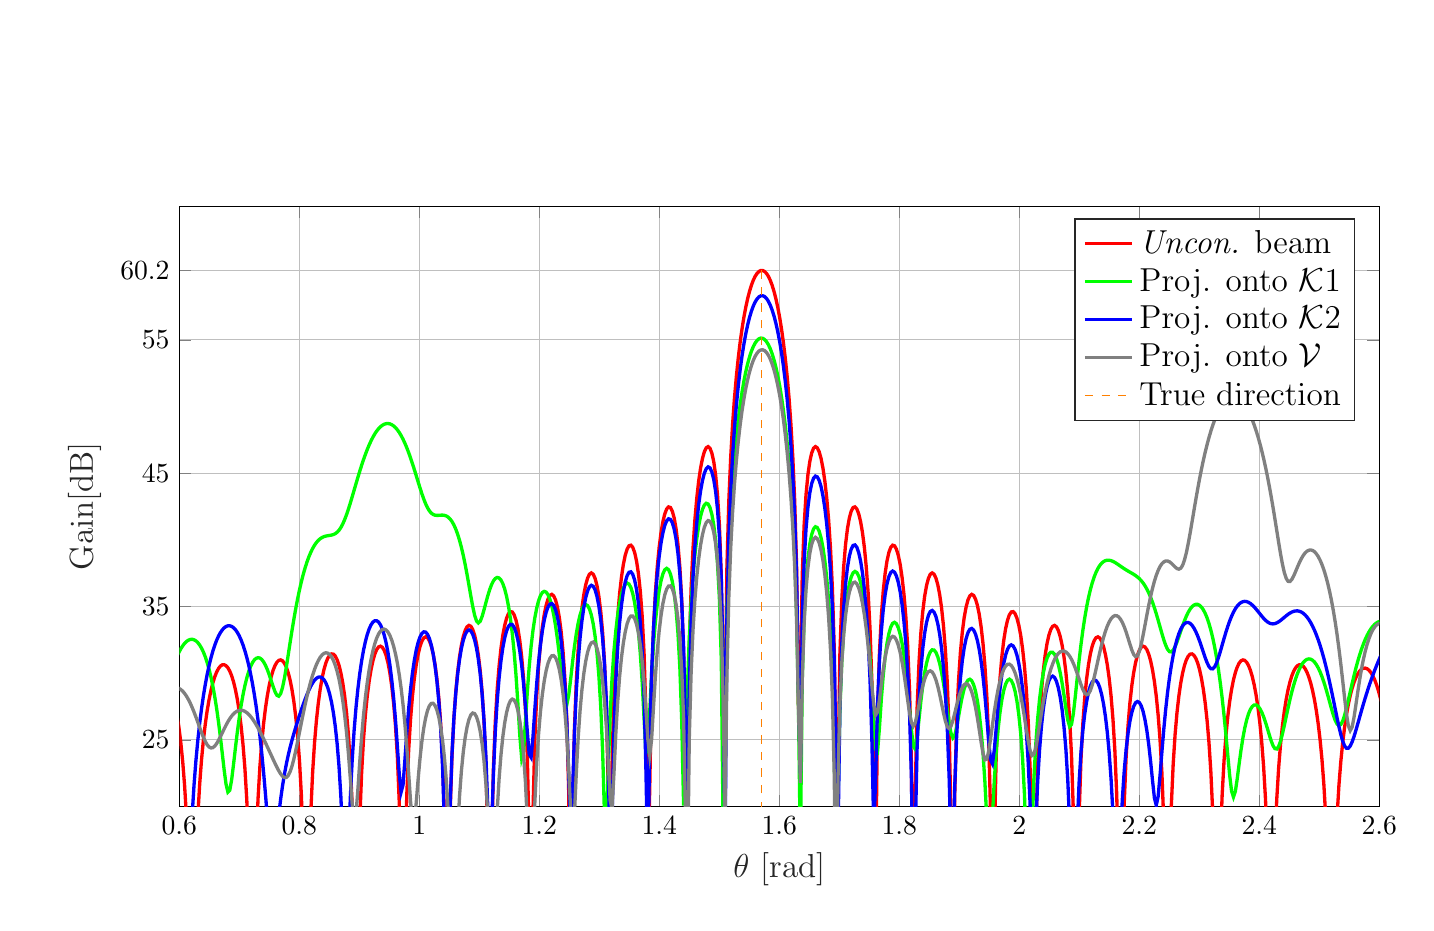
\begin{tikzpicture}

\begin{axis}[%
width=6in,
height=3in,
at={(0.758in,0.481in)},
scale only axis,
xmin=0.6,
xmax=2.6,
xlabel style={font=\large \color{white!15!black}},
xlabel={$\theta~[\mathrm{rad}]$},
ymin=20,
ymax=65,
ytick={ 25, 35, 45, 55, 60.2},
yminorticks=true,
ylabel style={font=\large \color{white!15!black}},
ylabel={Gain[$\mathrm{dB}$]},
xmajorgrids,
ymajorgrids,
axis background/.style={fill=white},
legend style={font = \large , legend cell align=left, align=left, draw=white!15!black}
]
\addplot [color=red, line width=1.2pt]
  table[row sep=crcr]{%
0.0031384541993904	-5.99642473721345\\
0.00627690839878081	-5.59279044739666\\
0.00941536259817121	-4.95915748418816\\
0.0125538167975616	-4.14323746599389\\
0.015692270996952	-3.19563650106894\\
0.0188307251963424	-2.16243734181925\\
0.0219691793957328	-1.0814627861472\\
0.0251076335951232	0.0184993235173993\\
0.0282460877945136	1.11678163471751\\
0.031384541993904	2.19927427748984\\
0.0345229961932944	3.25682329169867\\
0.0376614503926848	4.28385840435167\\
0.0407999045920752	5.27731956706988\\
0.0439383587914656	6.23586044939814\\
0.047076812990856	7.15927656796138\\
0.0502152671902464	8.04810349965607\\
0.0533537213896369	8.90333889422375\\
0.0564921755890272	9.72625248026996\\
0.0596306297884176	10.5182576978164\\
0.0627690839878081	11.2808260819861\\
0.0659075381871985	12.0154311099245\\
0.0690459923865889	12.723512247212\\
0.0721844465859793	13.4064527723371\\
0.0753229007853697	14.0655669424551\\
0.0784613549847601	14.7020934404967\\
0.0815998091841505	15.3171929962536\\
0.0847382633835409	15.9119487329294\\
0.0878767175829313	16.4873682448443\\
0.0910151717823217	17.0443867271398\\
0.0941536259817121	17.5838706959037\\
0.0972920801811025	18.1066219875674\\
0.100430534380493	18.6133818314151\\
0.103568988579883	19.104834859995\\
0.106707442779274	19.5816129731845\\
0.109845896978664	20.0442990046904\\
0.112984351178054	20.4934301637703\\
0.116122805377445	20.9295012399945\\
0.119261259576835	21.3529675696741\\
0.122399713776226	21.7642477690032\\
0.125538167975616	22.1637262431807\\
0.128676622175006	22.5517554832116\\
0.131815076374397	22.9286581631222\\
0.134953530573787	23.2947290508289\\
0.138091984773178	23.6502367457369\\
0.141230438972568	23.9954252554318\\
0.144368893171959	24.3305154234451\\
0.147507347371349	24.6557062188384\\
0.150645801570739	24.9711758977936\\
0.15378425577013	25.2770830461677\\
0.15692270996952	25.5735675112657\\
0.160061164168911	25.8607512300182\\
0.163199618368301	26.1387389599466\\
0.166338072567691	26.4076189184584\\
0.169476526767082	26.6674633351277\\
0.172614980966472	26.9183289208747\\
0.175753435165863	27.1602572572003\\
0.178891889365253	27.3932751077649\\
0.182030343564643	27.6173946540461\\
0.185168797764034	27.8326136557958\\
0.188307251963424	28.038915536516\\
0.191445706162815	28.2362693931334\\
0.194584160362205	28.4246299284066\\
0.197722614561595	28.6039373035381\\
0.200861068760986	28.7741169076904\\
0.203999522960376	28.9350790397812\\
0.207137977159767	29.0867184970219\\
0.210276431359157	29.2289140631176\\
0.213414885558547	29.3615278875989\\
0.216553339757938	29.4844047460709\\
0.219691793957328	29.5973711689518\\
0.222830248156719	29.7002344241094\\
0.225968702356109	29.7927813358385\\
0.229107156555499	29.8747769193435\\
0.23224561075489	29.9459628059495\\
0.23538406495428	30.0060554294603\\
0.238522519153671	30.0547439382996\\
0.241660973353061	30.0916877910874\\
0.244799427552451	30.1165139847333\\
0.247937881751842	30.1288138535385\\
0.251076335951232	30.1281393647675\\
0.254214790150623	30.1139988199147\\
0.257353244350013	30.0858518504113\\
0.260491698549403	30.043103570861\\
0.263630152748794	29.9850977201036\\
0.266768606948184	29.9111085784411\\
0.269907061147575	29.8203313951759\\
0.273045515346965	29.7118709899682\\
0.276183969546355	29.5847280986091\\
0.279322423745746	29.4377829104444\\
0.282460877945136	29.269775079131\\
0.285599332144527	29.0792792634935\\
0.288737786343917	28.8646749464016\\
0.291876240543307	28.6241088491647\\
0.295014694742698	28.355447650884\\
0.298153148942088	28.0562178491134\\
0.301291603141479	27.7235283228569\\
0.304430057340869	27.3539692597344\\
0.307568511540259	26.9434782208952\\
0.31070696573965	26.4871596188056\\
0.31384541993904	25.9790366897154\\
0.316983874138431	25.4117031891893\\
0.320122328337821	24.7758218282262\\
0.323260782537211	24.0593806247779\\
0.326399236736602	23.2465518012006\\
0.329537690935992	22.315867446172\\
0.332676145135383	21.2371534185208\\
0.335814599334773	19.9660451943425\\
0.338953053534163	18.4333618778399\\
0.342091507733554	16.5221918108681\\
0.345229961932944	14.0103708254357\\
0.348368416132335	10.3874055825086\\
0.351506870331725	3.94162169154461\\
0.354645324531115	-11.323735200797\\
0.357783778730506	5.92275912913403\\
0.360922232929896	11.4945859320992\\
0.364060687129287	14.8717420298159\\
0.367199141328677	17.2955651370578\\
0.370337595528067	19.1807945275579\\
0.373476049727458	20.7172530736311\\
0.376614503926848	22.0076991004429\\
0.379752958126239	23.1139855399087\\
0.382891412325629	24.0761768846061\\
0.38602986652502	24.921652784041\\
0.38916832072441	25.6698980869588\\
0.3923067749238	26.3352200631535\\
0.395445229123191	26.9283830924774\\
0.398583683322581	27.4576395274813\\
0.401722137521972	27.9294051964205\\
0.404860591721362	28.3487161951527\\
0.407999045920752	28.7195458128142\\
0.411137500120143	29.0450289488187\\
0.414275954319533	29.3276234410628\\
0.417414408518924	29.569227097261\\
0.420552862718314	29.7712626966834\\
0.423691316917704	29.9347390862001\\
0.426829771117095	30.0602937698159\\
0.429968225316485	30.1482205255195\\
0.433106679515876	30.1984842382001\\
0.436245133715266	30.2107240958602\\
0.439383587914656	30.184245407622\\
0.442522042114047	30.1179994473099\\
0.445660496313437	30.0105497937452\\
0.448798950512828	29.8600225004631\\
0.451937404712218	29.6640359121546\\
0.455075858911608	29.419603796907\\
0.458214313110999	29.1230022733322\\
0.461352767310389	28.7695860934205\\
0.46449122150978	28.353531996311\\
0.46762967570917	27.8674738970717\\
0.47076812990856	27.3019724963247\\
0.473906584107951	26.6447223215835\\
0.477045038307341	25.8793251638697\\
0.480183492506732	24.9833123697418\\
0.483321946706122	23.9247884640811\\
0.486460400905512	22.6563561922435\\
0.489598855104903	21.1031651625186\\
0.492737309304293	19.1366001429187\\
0.495875763503684	16.5061961873126\\
0.499014217703074	12.6117762607636\\
0.502152671902464	5.23745746943484\\
0.505291126101855	-2.27605395956505\\
0.508429580301245	10.132812585697\\
0.511568034500636	15.1205373271876\\
0.514706488700026	18.2551261538248\\
0.517844942899416	20.5276550540469\\
0.520983397098807	22.2950031257659\\
0.524121851298197	23.726357296748\\
0.527260305497588	24.9151554594333\\
0.530398759696978	25.9183051097434\\
0.533537213896368	26.7728871138124\\
0.536675668095759	27.5042627102058\\
0.539814122295149	28.1303961633243\\
0.54295257649454	28.6643285585839\\
0.54609103069393	29.1156726267643\\
0.54922948489332	29.4915543856439\\
0.552367939092711	29.7972244947812\\
0.555506393292101	30.036462353115\\
0.558644847491492	30.211843600711\\
0.561783301690882	30.3249125884796\\
0.564921755890272	30.3762842089006\\
0.568060210089663	30.3656885543981\\
0.571198664289053	30.2919641074452\\
0.574337118488444	30.1529986757642\\
0.577475572687834	29.9456106242078\\
0.580614026887224	29.6653546195524\\
0.583752481086615	29.3062239965242\\
0.586890935286005	28.8602024244746\\
0.590029389485396	28.3165841146346\\
0.593167843684786	27.6609207761652\\
0.596306297884177	26.8733354166647\\
0.599444752083567	25.9256990238806\\
0.602583206282957	24.7766208902219\\
0.605721660482348	23.3618607076904\\
0.608860114681738	21.5740203005118\\
0.611998568881128	19.2129262508794\\
0.615137023080519	15.8347648780968\\
0.618275477279909	10.0721624135129\\
0.6214139314793	-6.70975062072622\\
0.62455238567869	9.6070835367702\\
0.627690839878081	15.6791523928021\\
0.630829294077471	19.1973102645845\\
0.633967748276861	21.6529930066045\\
0.637106202476252	23.5152737594464\\
0.640244656675642	24.9923508305129\\
0.643383110875033	26.1946305275382\\
0.646521565074423	27.1874326053787\\
0.649660019273813	28.0123246779235\\
0.652798473473204	28.6971110711184\\
0.655936927672594	29.2610124682691\\
0.659075381871985	29.7175592848733\\
0.662213836071375	30.0762973342742\\
0.665352290270765	30.3438292699164\\
0.668490744470156	30.5244585503271\\
0.671629198669546	30.6205779252951\\
0.674767652868937	30.6328786598665\\
0.677906107068327	30.560418380068\\
0.681044561267717	30.4005593993334\\
0.684183015467108	30.148767006885\\
0.687321469666498	29.7982315993009\\
0.690459923865889	29.3392412663217\\
0.693598378065279	28.7581679454629\\
0.696736832264669	28.0358104729874\\
0.69987528646406	27.1445925240453\\
0.70301374066345	26.0435668928937\\
0.706152194862841	24.6688329707319\\
0.709290649062231	22.913219330122\\
0.712429103261621	20.5766216217084\\
0.715567557461012	17.2149768548988\\
0.718706011660402	11.4598648133945\\
0.721844465859793	-5.12398039620585\\
0.724982920059183	11.0264333875975\\
0.728121374258573	17.0775303347577\\
0.731259828457964	20.5756173773225\\
0.734398282657354	23.0056670329631\\
0.737536736856745	24.8354537477909\\
0.740675191056135	26.272549279588\\
0.743813645255525	27.4268461392179\\
0.746952099454916	28.3631225645266\\
0.750090553654306	29.1223183760128\\
0.753229007853697	29.7314838291563\\
0.756367462053087	30.2089197235292\\
0.759505916252478	30.5670235246989\\
0.762644370451868	30.8139336359272\\
0.765782824651258	30.9544877241121\\
0.768921278850649	30.990751067265\\
0.772059733050039	30.9222403533078\\
0.775198187249429	30.7458925205633\\
0.77833664144882	30.4557721062578\\
0.78147509564821	30.0424519238957\\
0.784613549847601	29.4919169117992\\
0.787752004046991	28.7836884801428\\
0.790890458246381	27.8875544852635\\
0.794028912445772	26.7575803408492\\
0.797167366645162	25.3202736138411\\
0.800305820844553	23.4485057946483\\
0.803444275043943	20.894130426468\\
0.806582729243334	17.0634200352198\\
0.809721183442724	9.78642418716504\\
0.812859637642114	2.17405552977874\\
0.815998091841505	14.5249513069887\\
0.819136546040895	19.4894642945522\\
0.822275000240286	22.5725079809793\\
0.825413454439676	24.7688173404618\\
0.828551908639066	26.4359569873461\\
0.831690362838457	27.7427457630106\\
0.834828817037847	28.7816956864225\\
0.837967271237237	29.6083554069802\\
0.841105725436628	30.2580181378877\\
0.844244179636018	30.753775101492\\
0.847382633835409	31.1107410234971\\
0.850521088034799	31.3383835602928\\
0.85365954223419	31.441811957609\\
0.85679799643358	31.422424136175\\
0.85993645063297	31.2780905528208\\
0.863074904832361	31.0029228005111\\
0.866213359031751	30.5865670201817\\
0.869351813231142	30.0128260921046\\
0.872490267430532	29.2571777626255\\
0.875628721629922	28.2822589045657\\
0.878767175829313	27.0291972556309\\
0.881905630028703	25.3994257644425\\
0.885044084228094	23.2111317644476\\
0.888182538427484	20.0713684643504\\
0.891320992626874	14.8384847780041\\
0.894459446826265	0.274370022608769\\
0.897597901025655	12.0960085216271\\
0.900736355225046	18.8077258229852\\
0.903874809424436	22.4997724263767\\
0.907013263623826	25.0026910253347\\
0.910151717823217	26.8499005789946\\
0.913290172022607	28.2698292551461\\
0.916428626221997	29.3806059569519\\
0.919567080421388	30.2504217136227\\
0.922705534620778	30.9213146045865\\
0.925843988820169	31.4200518144444\\
0.928982443019559	31.7636127965951\\
0.93212089721895	31.9621001507499\\
0.93525935141834	32.0202698941889\\
0.93839780561773	31.9382084308935\\
0.941536259817121	31.7113654101802\\
0.944674714016511	31.3299525543428\\
0.947813168215902	30.7775248578319\\
0.950951622415292	30.0282635735338\\
0.954090076614682	29.0418740116665\\
0.957228530814073	27.7535430611645\\
0.960366985013463	26.0522748276261\\
0.963505439212854	23.7269952979944\\
0.966643893412244	20.298366059948\\
0.969782347611634	14.219145259356\\
0.972920801811025	-2.20101666629497\\
0.976059256010415	15.1714923127127\\
0.979197710209806	20.8867105885086\\
0.982336164409196	24.2368076686069\\
0.985474618608586	26.5551610071732\\
0.988613072807977	28.2763520938451\\
0.991751527007367	29.5958321353501\\
0.994889981206758	30.6172981696937\\
0.998028435406148	31.4012970698969\\
1.00116688960554	31.9850784686539\\
1.00430534380493	32.3918594837653\\
1.00744379800432	32.6355022884974\\
1.01058225220371	32.72291732592\\
1.0137207064031	32.6551613279512\\
1.01685916060249	32.4276172610672\\
1.01999761480188	32.029316373601\\
1.02313606900127	31.4411722009835\\
1.02627452320066	30.6324614170876\\
1.02941297740005	29.5539720481459\\
1.03255143159944	28.1239031279139\\
1.03568988579883	26.1955178596638\\
1.03882833999822	23.4688744330468\\
1.04196679419761	19.1677488882772\\
1.045105248397	9.78957218204447\\
1.04824370259639	10.3187773529512\\
1.05138215679578	19.4701448803219\\
1.05452061099518	23.7906287627366\\
1.05765906519457	26.5735719521642\\
1.06079751939396	28.5690351379741\\
1.06393597359335	30.0691910029995\\
1.06707442779274	31.2172422023329\\
1.07021288199213	32.0927823080268\\
1.07335133619152	32.7432451539382\\
1.07648979039091	33.1976247700772\\
1.0796282445903	33.4730960932381\\
1.08276669878969	33.578324897076\\
1.08590515298908	33.5149746931862\\
1.08904360718847	33.2780001117058\\
1.09218206138786	32.8548342134291\\
1.09532051558725	32.2231674593306\\
1.09845896978664	31.3463968897479\\
1.10159742398603	30.164466259761\\
1.10473587818542	28.5741347215628\\
1.10787433238481	26.3805931370699\\
1.1110127865842	23.1506465744851\\
1.11415124078359	17.5536306890568\\
1.11728969498298	-0.939044300589249\\
1.12042814918237	16.6532628702645\\
1.12356660338176	22.8664043483735\\
1.12670505758115	26.3786015773713\\
1.12984351178054	28.7682443099258\\
1.13298196597994	30.5186534164586\\
1.13612042017933	31.8410123147082\\
1.13925887437872	32.8451627503388\\
1.14239732857811	33.5939983589673\\
1.1455357827775	34.1251687856398\\
1.14867423697689	34.460978434897\\
1.15181269117628	34.6131979514573\\
1.15495114537567	34.585299568483\\
1.15808959957506	34.3730894561285\\
1.16122805377445	33.963988147863\\
1.16436650797384	33.3346733538012\\
1.16750496217323	32.4460509041734\\
1.17064341637262	31.2328933364674\\
1.17378187057201	29.5809797539565\\
1.1769203247714	27.2691749573679\\
1.18005877897079	23.7840275080282\\
1.18319723317018	17.3866159470385\\
1.18633568736957	2.23246610609685\\
1.18947414156896	19.5563217561513\\
1.19261259576835	25.044703640786\\
1.19575104996774	28.2999656112989\\
1.19888950416713	30.5514646359984\\
1.20202795836652	32.209238747032\\
1.20516641256591	33.4593104028549\\
1.20830486676531	34.4002473624819\\
1.2114433209647	35.088789183132\\
1.21458177516409	35.5585408404854\\
1.21772022936348	35.8285767726603\\
1.22085868356287	35.9075362913161\\
1.22399713776226	35.7953007638793\\
1.22713559196165	35.4829893718659\\
1.23027404616104	34.9512720537388\\
1.23341250036043	34.1662589171234\\
1.23655095455982	33.0708668126739\\
1.23968940875921	31.566055666466\\
1.2428278629586	29.4649916586895\\
1.24596631715799	26.3556147737461\\
1.24910477135738	20.9987918265153\\
1.25224322555677	3.18347585807228\\
1.25538167975616	19.1677389126804\\
1.25852013395555	25.7017415180474\\
1.26165858815494	29.3210585500119\\
1.26479704235433	31.7640085201338\\
1.26793549655372	33.5427112332752\\
1.27107395075311	34.8771759023327\\
1.2742124049525	35.8804463429662\\
1.27735085915189	36.6163683076682\\
1.28048931335128	37.1223112595796\\
1.28362776755067	37.4193546480614\\
1.28676622175007	37.517057189851\\
1.28990467594946	37.415396841456\\
1.29304313014885	37.104779572879\\
1.29618158434824	36.5641211061776\\
1.29932003854763	35.7561151910564\\
1.30245849274702	34.6171270827446\\
1.30559694694641	33.0346703569096\\
1.3087354011458	30.7902354286869\\
1.31187385534519	27.3765132067596\\
1.31501230954458	21.079226881473\\
1.31815076374397	3.97958276234809\\
1.32128921794336	23.0808894835216\\
1.32442767214275	28.6673183957377\\
1.32756612634214	31.9714916695417\\
1.33070458054153	34.2558661367544\\
1.33384303474092	35.9368286263759\\
1.33698148894031	37.2021528771398\\
1.3401199431397	38.1506969741513\\
1.34325839733909	38.8387553427442\\
1.34639685153848	39.2989131909547\\
1.34953530573787	39.5485946476929\\
1.35267375993726	39.5939443997073\\
1.35581221413665	39.4310861297623\\
1.35895066833604	39.0453428816137\\
1.36208912253543	38.408061886562\\
1.36522757673483	37.4694344671798\\
1.36836603093422	36.1428489611712\\
1.37150448513361	34.2676388341318\\
1.374642939333	31.5029935858803\\
1.37778139353239	26.9091533706949\\
1.38091984773178	15.1457493462071\\
1.38405830193117	21.2447193562665\\
1.38719675613056	29.2412399561374\\
1.39033521032995	33.3149633850734\\
1.39347366452934	36.0051339281156\\
1.39661211872873	37.952769560116\\
1.39975057292812	39.417307503955\\
1.40288902712751	40.5277768033799\\
1.4060274813269	41.3555618436253\\
1.40916593552629	41.9418196250381\\
1.41230438972568	42.3094201189637\\
1.41544284392507	42.4684023409788\\
1.41858129812446	42.4181018950932\\
1.42171975232385	42.1469964024216\\
1.42485820652324	41.6301964009203\\
1.42799666072263	40.8233265848772\\
1.43113511492202	39.6491430549765\\
1.43427356912141	37.9663278965806\\
1.4374120233208	35.4842196715461\\
1.44055047752019	31.452028270216\\
1.44368893171959	22.4774047759838\\
1.44682738591898	21.8615361092675\\
1.44996584011837	31.8235226841921\\
1.45310429431776	36.4009934425059\\
1.45624274851715	39.3658193693887\\
1.45938120271654	41.5115798989144\\
1.46251965691593	43.1409127463643\\
1.46565811111532	44.3999905847928\\
1.46879656531471	45.368528675793\\
1.4719350195141	46.0923758667925\\
1.47507347371349	46.5973936665219\\
1.47821192791288	46.8957636153592\\
1.48135038211227	46.988544432933\\
1.48448883631166	46.8657743077395\\
1.48762729051105	46.5041633422756\\
1.49076574471044	45.8612109884595\\
1.49390419890983	44.86224062049\\
1.49704265310922	43.3702086690398\\
1.50018110730861	41.1037240394306\\
1.503319561508	37.3420909548975\\
1.50645801570739	28.9298569972887\\
1.50959646990678	27.2912922647064\\
1.51273492410617	37.9651007409201\\
1.51587337830556	42.8850563928396\\
1.51901183250496	46.1633325412505\\
1.52215028670435	48.6307920715399\\
1.52528874090374	50.6030121801656\\
1.52842719510313	52.2343531556686\\
1.53156564930252	53.6120095421643\\
1.53470410350191	54.7900811865057\\
1.5378425577013	55.8044155237558\\
1.54098101190069	56.6799324749848\\
1.54411946610008	57.4345825056953\\
1.54725792029947	58.0816378686069\\
1.55039637449886	58.6310920681425\\
1.55353482869825	59.0905514016513\\
1.55667328289764	59.4658216359222\\
1.55981173709703	59.7613030871914\\
1.56295019129642	59.9802600090412\\
1.56608864549581	60.1250038520518\\
1.5692270996952	60.1970145589734\\
1.57236555389459	60.1970145589734\\
1.57550400809398	60.1250038520518\\
1.57864246229337	59.9802600090412\\
1.58178091649276	59.7613030871914\\
1.58491937069215	59.4658216359222\\
1.58805782489154	59.0905514016513\\
1.59119627909093	58.6310920681424\\
1.59433473329032	58.0816378686068\\
1.59747318748972	57.4345825056953\\
1.60061164168911	56.6799324749848\\
1.6037500958885	55.8044155237559\\
1.60688855008789	54.7900811865057\\
1.61002700428728	53.6120095421641\\
1.61316545848667	52.2343531556686\\
1.61630391268606	50.6030121801656\\
1.61944236688545	48.6307920715399\\
1.62258082108484	46.1633325412502\\
1.62571927528423	42.8850563928398\\
1.62885772948362	37.9651007409195\\
1.63199618368301	27.2912922647074\\
1.6351346378824	28.9298569972888\\
1.63827309208179	37.3420909548972\\
1.64141154628118	41.1037240394306\\
1.64455000048057	43.3702086690398\\
1.64768845467996	44.8622406204899\\
1.65082690887935	45.8612109884596\\
1.65396536307874	46.5041633422755\\
1.65710381727813	46.8657743077394\\
1.66024227147752	46.9885444329329\\
1.66338072567691	46.8957636153593\\
1.6665191798763	46.5973936665218\\
1.66965763407569	46.0923758667927\\
1.67279608827508	45.368528675793\\
1.67593454247447	44.3999905847928\\
1.67907299667387	43.1409127463645\\
1.68221145087326	41.5115798989142\\
1.68534990507265	39.3658193693885\\
1.68848835927204	36.4009934425061\\
1.69162681347143	31.823522684192\\
1.69476526767082	21.8615361092671\\
1.69790372187021	22.4774047759863\\
1.7010421760696	31.4520282702167\\
1.70418063026899	35.4842196715466\\
1.70731908446838	37.9663278965805\\
1.71045753866777	39.6491430549762\\
1.71359599286716	40.8233265848775\\
1.71673444706655	41.6301964009204\\
1.71987290126594	42.1469964024218\\
1.72301135546533	42.4181018950932\\
1.72614980966472	42.4684023409789\\
1.72928826386411	42.3094201189637\\
1.7324267180635	41.9418196250381\\
1.73556517226289	41.3555618436253\\
1.73870362646228	40.52777680338\\
1.74184208066167	39.4173075039547\\
1.74498053486106	37.9527695601154\\
1.74811898906045	36.0051339281155\\
1.75125744325984	33.3149633850736\\
1.75439589745924	29.2412399561374\\
1.75753435165863	21.2447193562666\\
1.76067280585802	15.1457493462072\\
1.76381126005741	26.9091533706949\\
1.7669497142568	31.5029935858803\\
1.77008816845619	34.2676388341318\\
1.77322662265558	36.1428489611705\\
1.77636507685497	37.4694344671804\\
1.77950353105436	38.408061886562\\
1.78264198525375	39.0453428816137\\
1.78578043945314	39.4310861297623\\
1.78891889365253	39.5939443997075\\
1.79205734785192	39.5485946476927\\
1.79519580205131	39.2989131909547\\
1.7983342562507	38.8387553427442\\
1.80147271045009	38.1506969741516\\
1.80461116464948	37.2021528771396\\
1.80774961884887	35.9368286263759\\
1.81088807304826	34.2558661367545\\
1.81402652724765	31.9714916695417\\
1.81716498144704	28.6673183957377\\
1.82030343564643	23.0808894835223\\
1.82344188984582	3.97958276235981\\
1.82658034404521	21.0792268814735\\
1.8297187982446	27.3765132067593\\
1.83285725244399	30.7902354286866\\
1.83599570664339	33.0346703569094\\
1.83913416084278	34.6171270827443\\
1.84227261504217	35.7561151910561\\
1.84541106924156	36.5641211061777\\
1.84854952344095	37.1047795728788\\
1.85168797764034	37.4153968414559\\
1.85482643183973	37.517057189851\\
1.85796488603912	37.4193546480611\\
1.86110334023851	37.1223112595802\\
1.8642417944379	36.6163683076675\\
1.86738024863729	35.8804463429669\\
1.87051870283668	34.8771759023328\\
1.87365715703607	33.5427112332751\\
1.87679561123546	31.7640085201348\\
1.87993406543485	29.321058550013\\
1.88307251963424	25.7017415180481\\
1.88621097383363	19.167738912678\\
1.88934942803302	3.18347585807074\\
1.89248788223241	20.9987918265142\\
1.8956263364318	26.3556147737466\\
1.89876479063119	29.4649916586884\\
1.90190324483058	31.5660556664659\\
1.90504169902997	33.0708668126739\\
1.90818015322936	34.1662589171232\\
1.91131860742876	34.9512720537389\\
1.91445706162815	35.482989371865\\
1.91759551582754	35.795300763879\\
1.92073397002693	35.9075362913159\\
1.92387242422632	35.8285767726602\\
1.92701087842571	35.5585408404855\\
1.9301493326251	35.0887891831322\\
1.93328778682449	34.4002473624822\\
1.93642624102388	33.4593104028549\\
1.93956469522327	32.209238747032\\
1.94270314942266	30.5514646359982\\
1.94584160362205	28.2999656112985\\
1.94898005782144	25.0447036407854\\
1.95211851202083	19.5563217561535\\
1.95525696622022	2.23246610609551\\
1.95839542041961	17.3866159470378\\
1.961533874619	23.7840275080259\\
1.96467232881839	27.2691749573674\\
1.96781078301778	29.5809797539548\\
1.97094923721717	31.2328933364672\\
1.97408769141656	32.4460509041735\\
1.97722614561595	33.3346733538022\\
1.98036459981534	33.9639881478635\\
1.98350305401473	34.3730894561285\\
1.98664150821412	34.5852995684829\\
1.98977996241352	34.6131979514575\\
1.99291841661291	34.460978434897\\
1.9960568708123	34.1251687856398\\
1.99919532501169	33.5939983589671\\
2.00233377921108	32.8451627503385\\
2.00547223341047	31.8410123147083\\
2.00861068760986	30.5186534164591\\
2.01174914180925	28.7682443099258\\
2.01488759600864	26.3786015773691\\
2.01802605020803	22.8664043483766\\
2.02116450440742	16.6532628702715\\
2.02430295860681	-0.939044300609283\\
2.0274414128062	17.5536306890563\\
2.03057986700559	23.150646574486\\
2.03371832120498	26.3805931370706\\
2.03685677540437	28.5741347215627\\
2.03999522960376	30.1644662597596\\
2.04313368380315	31.3463968897477\\
2.04627213800254	32.2231674593312\\
2.04941059220193	32.8548342134288\\
2.05254904640132	33.2780001117057\\
2.05568750060071	33.5149746931861\\
2.0588259548001	33.5783248970762\\
2.06196440899949	33.4730960932379\\
2.06510286319888	33.197624770077\\
2.06824131739828	32.7432451539379\\
2.07137977159767	32.0927823080273\\
2.07451822579706	31.2172422023325\\
2.07765667999645	30.0691910029987\\
2.08079513419584	28.5690351379751\\
2.08393358839523	26.5735719521646\\
2.08707204259462	23.790628762733\\
2.09021049679401	19.4701448803253\\
2.0933489509934	10.3187773529475\\
2.09648740519279	9.78957218204449\\
2.09962585939218	19.1677488882772\\
2.10276431359157	23.4688744330477\\
2.10590276779096	26.1955178596633\\
2.10904122199035	28.1239031279139\\
2.11217967618974	29.5539720481464\\
2.11531813038913	30.6324614170874\\
2.11845658458852	31.4411722009841\\
2.12159503878791	32.0293163736016\\
2.1247334929873	32.4276172610672\\
2.12787194718669	32.6551613279518\\
2.13101040138608	32.7229173259201\\
2.13414885558547	32.6355022884974\\
2.13728730978486	32.3918594837655\\
2.14042576398425	31.9850784686538\\
2.14356421818364	31.4012970698967\\
2.14670267238304	30.6172981696937\\
2.14984112658243	29.5958321353501\\
2.15297958078182	28.2763520938424\\
2.15611803498121	26.5551610071742\\
2.1592564891806	24.236807668608\\
2.16239494337999	20.8867105885092\\
2.16553339757938	15.1714923127132\\
2.16867185177877	-2.20101666629538\\
2.17181030597816	14.219145259355\\
2.17494876017755	20.2983660599495\\
2.17808721437694	23.7269952979946\\
2.18122566857633	26.0522748276273\\
2.18436412277572	27.7535430611646\\
2.18750257697511	29.0418740116662\\
2.1906410311745	30.0282635735337\\
2.19377948537389	30.7775248578327\\
2.19691793957328	31.3299525543425\\
2.20005639377267	31.7113654101804\\
2.20319484797206	31.9382084308944\\
2.20633330217145	32.0202698941888\\
2.20947175637084	31.9621001507495\\
2.21261021057023	31.7636127965956\\
2.21574866476962	31.4200518144453\\
2.21888711896901	30.9213146045865\\
2.22202557316841	30.2504217136228\\
2.2251640273678	29.3806059569523\\
2.22830248156719	28.2698292551455\\
2.23144093576658	26.8499005789954\\
2.23457938996597	25.0026910253345\\
2.23771784416536	22.499772426375\\
2.24085629836475	18.8077258229839\\
2.24399475256414	12.0960085216342\\
2.24713320676353	0.274370022597165\\
2.25027166096292	14.8384847780051\\
2.25341011516231	20.071368464352\\
2.2565485693617	23.2111317644491\\
2.25968702356109	25.3994257644426\\
2.26282547776048	27.0291972556307\\
2.26596393195987	28.2822589045656\\
2.26910238615926	29.2571777626256\\
2.27224084035865	30.0128260921042\\
2.27537929455804	30.5865670201817\\
2.27851774875743	31.0029228005111\\
2.28165620295682	31.2780905528208\\
2.28479465715621	31.4224241361749\\
2.2879331113556	31.441811957609\\
2.29107156555499	31.3383835602927\\
2.29421001975438	31.1107410234976\\
2.29734847395377	30.7537751014913\\
2.30048692815316	30.258018137889\\
2.30362538235256	29.6083554069812\\
2.30676383655195	28.7816956864224\\
2.30990229075134	27.7427457630106\\
2.31304074495073	26.435956987346\\
2.31617919915012	24.7688173404624\\
2.31931765334951	22.57250798098\\
2.3224561075489	19.4894642945517\\
2.32559456174829	14.5249513069868\\
2.32873301594768	2.17405552979971\\
2.33187147014707	9.78642418716181\\
2.33500992434646	17.0634200352129\\
2.33814837854585	20.894130426467\\
2.34128683274524	23.4485057946485\\
2.34442528694463	25.3202736138414\\
2.34756374114402	26.7575803408492\\
2.35070219534341	27.8875544852636\\
2.3538406495428	28.7836884801427\\
2.35697910374219	29.4919169117991\\
2.36011755794158	30.0424519238957\\
2.36325601214097	30.4557721062575\\
2.36639446634036	30.7458925205639\\
2.36953292053975	30.9222403533071\\
2.37267137473914	30.9907510672651\\
2.37580982893853	30.9544877241124\\
2.37894828313792	30.813933635926\\
2.38208673733732	30.5670235246989\\
2.38522519153671	30.2089197235283\\
2.3883636457361	29.7314838291563\\
2.39150209993549	29.1223183760122\\
2.39464055413488	28.3631225645261\\
2.39777900833427	27.4268461392184\\
2.40091746253366	26.2725492795876\\
2.40405591673305	24.8354537477918\\
2.40719437093244	23.0056670329637\\
2.41033282513183	20.5756173773155\\
2.41347127933122	17.0775303347546\\
2.41660973353061	11.0264333875839\\
2.41974818773	-5.12398039618781\\
2.42288664192939	11.459864813396\\
2.42602509612878	17.2149768548937\\
2.42916355032817	20.5766216217069\\
2.43230200452756	22.9132193301233\\
2.43544045872695	24.6688329707321\\
2.43857891292634	26.043566892894\\
2.44171736712573	27.144592524045\\
2.44485582132512	28.0358104729871\\
2.44799427552451	28.7581679454622\\
2.4511327297239	29.3392412663215\\
2.4542711839233	29.7982315993006\\
2.45740963812269	30.1487670068855\\
2.46054809232208	30.4005593993339\\
2.46368654652147	30.5604183800682\\
2.46682500072086	30.6328786598664\\
2.46996345492025	30.6205779252952\\
2.47310190911964	30.5244585503274\\
2.47624036331903	30.3438292699175\\
2.47937881751842	30.0762973342745\\
2.48251727171781	29.7175592848733\\
2.4856557259172	29.261012468269\\
2.48879418011659	28.69711107112\\
2.49193263431598	28.0123246779228\\
2.49507108851537	27.1874326053765\\
2.49820954271476	26.1946305275381\\
2.50134799691415	24.9923508305122\\
2.50448645111354	23.5152737594448\\
2.50762490531293	21.6529930066028\\
2.51076335951232	19.1973102645836\\
2.51390181371171	15.6791523928025\\
2.5170402679111	9.60708353676999\\
2.52017872211049	-6.70975062072361\\
2.52331717630988	10.0721624135092\\
2.52645563050927	15.834764878097\\
2.52959408470866	19.2129262508784\\
2.53273253890806	21.5740203005118\\
2.53587099310745	23.3618607076904\\
2.53900944730684	24.7766208902216\\
2.54214790150623	25.9256990238808\\
2.54528635570562	26.8733354166646\\
2.54842480990501	27.660920776166\\
2.5515632641044	28.3165841146338\\
2.55470171830379	28.8602024244744\\
2.55784017250318	29.3062239965245\\
2.56097862670257	29.6653546195522\\
2.56411708090196	29.9456106242071\\
2.56725553510135	30.1529986757642\\
2.57039398930074	30.291964107445\\
2.57353244350013	30.3656885543989\\
2.57667089769952	30.376284208901\\
2.57980935189891	30.3249125884798\\
2.5829478060983	30.2118436007104\\
2.58608626029769	30.0364623531147\\
2.58922471449708	29.7972244947826\\
2.59236316869647	29.4915543856435\\
2.59550162289586	29.1156726267644\\
2.59864007709525	28.6643285585842\\
2.60177853129464	28.1303961633236\\
2.60491698549403	27.5042627102062\\
2.60805543969342	26.7728871138126\\
2.61119389389282	25.918305109743\\
2.61433234809221	24.9151554594333\\
2.6174708022916	23.7263572967485\\
2.62060925649099	22.2950031257663\\
2.62374771069038	20.5276550540437\\
2.62688616488977	18.2551261538254\\
2.63002461908916	15.120537327186\\
2.63316307328855	10.1328125857059\\
2.63630152748794	-2.27605395956192\\
2.63943998168733	5.23745746945069\\
2.64257843588672	12.6117762607653\\
2.64571689008611	16.5061961873147\\
2.6488553442855	19.1366001429193\\
2.65199379848489	21.1031651625219\\
2.65513225268428	22.656356192242\\
2.65827070688367	23.9247884640818\\
2.66140916108306	24.9833123697418\\
2.66454761528245	25.8793251638708\\
2.66768606948184	26.6447223215837\\
2.67082452368123	27.3019724963248\\
2.67396297788062	27.8674738970711\\
2.67710143208001	28.3535319963121\\
2.6802398862794	28.7695860934211\\
2.68337834047879	29.1230022733322\\
2.68651679467818	29.419603796907\\
2.68965524887758	29.6640359121522\\
2.69279370307697	29.8600225004626\\
2.69593215727636	30.0105497937452\\
2.69907061147575	30.1179994473096\\
2.70220906567514	30.1842454076215\\
2.70534751987453	30.2107240958594\\
2.70848597407392	30.1984842381997\\
2.71162442827331	30.1482205255199\\
2.7147628824727	30.0602937698151\\
2.71790133667209	29.9347390861999\\
2.72103979087148	29.7712626966832\\
2.72417824507087	29.5692270972602\\
2.72731669927026	29.3276234410628\\
2.73045515346965	29.0450289488185\\
2.73359360766904	28.7195458128137\\
2.73673206186843	28.3487161951522\\
2.73987051606782	27.9294051964195\\
2.74300897026721	27.4576395274812\\
2.7461474244666	26.9283830924767\\
2.74928587866599	26.3352200631527\\
2.75242433286538	25.6698980869585\\
2.75556278706477	24.921652784039\\
2.75870124126416	24.0761768846045\\
2.76183969546355	23.1139855399092\\
2.76497814966294	22.0076991004406\\
2.76811660386234	20.7172530736326\\
2.77125505806173	19.1807945275577\\
2.77439351226112	17.2955651370532\\
2.77753196646051	14.8717420298125\\
2.7806704206599	11.4945859320987\\
2.78380887485929	5.92275912912749\\
2.78694732905868	-11.3237352006504\\
2.79008578325807	3.94162169154872\\
2.79322423745746	10.3874055825055\\
2.79636269165685	14.0103708254397\\
2.79950114585624	16.5221918108691\\
2.80263960005563	18.4333618778402\\
2.80577805425502	19.9660451943448\\
2.80891650845441	21.2371534185201\\
2.8120549626538	22.315867446173\\
2.81519341685319	23.2465518012011\\
2.81833187105258	24.0593806247786\\
2.82147032525197	24.7758218282263\\
2.82460877945136	25.4117031891903\\
2.82774723365075	25.9790366897154\\
2.83088568785014	26.487159618805\\
2.83402414204953	26.9434782208956\\
2.83716259624892	27.3539692597334\\
2.84030105044831	27.7235283228573\\
2.84343950464771	28.0562178491136\\
2.8465779588471	28.3554476508844\\
2.84971641304649	28.6241088491648\\
2.85285486724588	28.8646749464021\\
2.85599332144527	29.0792792634933\\
2.85913177564466	29.2697750791312\\
2.86227022984405	29.4377829104445\\
2.86540868404344	29.5847280986102\\
2.86854713824283	29.7118709899685\\
2.87168559244222	29.8203313951763\\
2.87482404664161	29.9111085784421\\
2.877962500841	29.9850977201037\\
2.88110095504039	30.0431035708625\\
2.88423940923978	30.0858518504117\\
2.88737786343917	30.1139988199152\\
2.89051631763856	30.1281393647678\\
2.89365477183795	30.128813853539\\
2.89679322603734	30.1165139847335\\
2.89993168023673	30.0916877910875\\
2.90307013443612	30.0547439383004\\
2.90620858863551	30.0060554294624\\
2.9093470428349	29.9459628059492\\
2.91248549703429	29.8747769193436\\
2.91562395123368	29.7927813358387\\
2.91876240543307	29.7002344241098\\
2.92190085963247	29.5973711689522\\
2.92503931383186	29.4844047460717\\
2.92817776803125	29.3615278875995\\
2.93131622223064	29.2289140631185\\
2.93445467643003	29.0867184970233\\
2.93759313062942	28.9350790397807\\
2.94073158482881	28.7741169076909\\
2.9438700390282	28.6039373035382\\
2.94700849322759	28.4246299284062\\
2.95014694742698	28.2362693931364\\
2.95328540162637	28.0389155365156\\
2.95642385582576	27.8326136557964\\
2.95956231002515	27.6173946540462\\
2.96270076422454	27.3932751077685\\
2.96583921842393	27.1602572572007\\
2.96897767262332	26.918328920876\\
2.97211612682271	26.6674633351276\\
2.9752545810221	26.4076189184595\\
2.97839303522149	26.1387389599473\\
2.98153148942088	25.8607512300169\\
2.98466994362027	25.5735675112663\\
2.98780839781966	25.2770830461687\\
2.99094685201905	24.971175897793\\
2.99408530621844	24.6557062188392\\
2.99722376041783	24.3305154234457\\
3.00036221461722	23.9954252554349\\
3.00350066881662	23.6502367457379\\
3.00663912301601	23.2947290508271\\
3.0097775772154	22.9286581631221\\
3.01291603141479	22.551755483211\\
3.01605448561418	22.1637262431793\\
3.01919293981357	21.7642477690052\\
3.02233139401296	21.3529675696743\\
3.02546984821235	20.9295012399986\\
3.02860830241174	20.4934301637702\\
3.03174675661113	20.0442990046901\\
3.03488521081052	19.5816129731872\\
3.03802366500991	19.1048348599983\\
3.0411621192093	18.6133818314156\\
3.04430057340869	18.1066219875681\\
3.04743902760808	17.5838706959042\\
3.05057748180747	17.0443867271411\\
3.05371593600686	16.4873682448503\\
3.05685439020625	15.9119487329306\\
3.05999284440564	15.3171929962516\\
3.06313129860503	14.702093440502\\
3.06626975280442	14.0655669424529\\
3.06940820700381	13.4064527723365\\
3.0725466612032	12.7235122472142\\
3.07568511540259	12.0154311099275\\
3.07882356960198	11.2808260819789\\
3.08196202380138	10.5182576978154\\
3.08510047800077	9.72625248027149\\
3.08823893220016	8.90333889422046\\
3.09137738639955	8.04810349965129\\
3.09451584059894	7.15927656795838\\
3.09765429479833	6.23586044939264\\
3.10079274899772	5.27731956707846\\
3.10393120319711	4.2838584043466\\
3.1070696573965	3.25682329169262\\
3.11020811159589	2.19927427749555\\
3.11334656579528	1.11678163471759\\
3.11648501999467	0.0184993235256842\\
3.11962347419406	-1.08146278616598\\
3.12276192839345	-2.16243734182967\\
3.12590038259284	-3.19563650105281\\
3.12903883679223	-4.14323746598748\\
3.13217729099162	-4.95915748416796\\
3.13531574519101	-5.59279044744455\\
3.1384541993904	-5.99642473722975\\
};
\addlegendentry{\emph{Uncon.} beam}

\addplot [color=green, line width=1.2pt]
  table[row sep=crcr]{%
0.0031384541993904	30.4362311869824\\
0.00627690839878081	30.434102661184\\
0.00941536259817121	30.4305451705098\\
0.0125538167975616	30.4255437789416\\
0.015692270996952	30.4190775468783\\
0.0188307251963424	30.4111195015628\\
0.0219691793957328	30.401636598467\\
0.0251076335951232	30.3905896732265\\
0.0282460877945136	30.3779333835472\\
0.031384541993904	30.363616140462\\
0.0345229961932944	30.347580028128\\
0.0376614503926848	30.3297607113299\\
0.0407999045920752	30.3100873296252\\
0.0439383587914656	30.288482376985\\
0.047076812990856	30.2648615656562\\
0.0502152671902464	30.239133672746\\
0.0533537213896369	30.2112003678975\\
0.0564921755890272	30.1809560202515\\
0.0596306297884176	30.1482874826241\\
0.0627690839878081	30.1130738506542\\
0.0659075381871985	30.0751861943956\\
0.0690459923865889	30.0344872595476\\
0.0721844465859793	29.9908311352232\\
0.0753229007853697	29.9440628847743\\
0.0784613549847601	29.8940181358614\\
0.0815998091841505	29.8405226254764\\
0.0847382633835409	29.7833916951632\\
0.0878767175829313	29.7224297311941\\
0.0910151717823217	29.6574295437944\\
0.0941536259817121	29.5881716789425\\
0.0972920801811025	29.5144236554992\\
0.100430534380493	29.4359391196287\\
0.103568988579883	29.3524569076993\\
0.106707442779274	29.2637000078414\\
0.109845896978664	29.1693744094501\\
0.112984351178054	29.0691678288676\\
0.116122805377445	28.9627482985708\\
0.119261259576835	28.8497626061902\\
0.122399713776226	28.7298345690246\\
0.125538167975616	28.602563129196\\
0.128676622175006	28.467520254756\\
0.131815076374397	28.3242486329301\\
0.134953530573787	28.1722591440562\\
0.138091984773178	28.0110281090296\\
0.141230438972568	27.8399943107077\\
0.144368893171959	27.6585558018296\\
0.147507347371349	27.4660665314808\\
0.150645801570739	27.2618328520534\\
0.15378425577013	27.0451100145745\\
0.15692270996952	26.8150988299658\\
0.160061164168911	26.5709427791685\\
0.163199618368301	26.3117260138912\\
0.166338072567691	26.0364729292246\\
0.169476526767082	25.7441503503827\\
0.172614980966472	25.4336739204674\\
0.175753435165863	25.1039210985496\\
0.178891889365253	24.7537544188337\\
0.182030343564643	24.3820605319346\\
0.185168797764034	23.9878133527278\\
0.188307251963424	23.5701737953246\\
0.191445706162815	23.1286446141718\\
0.194584160362205	22.663307317985\\
0.197722614561595	22.1751791184622\\
0.200861068760986	21.6667401005275\\
0.203999522960376	21.1426889694374\\
0.207137977159767	20.6109754571455\\
0.210276431359157	20.0840969653914\\
0.213414885558547	19.5804802258901\\
0.216553339757938	19.1254319592266\\
0.219691793957328	18.7506579730822\\
0.222830248156719	18.4910397528229\\
0.225968702356109	18.3779842289804\\
0.229107156555499	18.4308300014413\\
0.23224561075489	18.6503741437785\\
0.23538406495428	19.0185471145517\\
0.238522519153671	19.5044553195027\\
0.241660973353061	20.0729776078262\\
0.244799427552451	20.6916986594118\\
0.247937881751842	21.3344390275068\\
0.251076335951232	21.9819323413126\\
0.254214790150623	22.6209562408839\\
0.257353244350013	23.2429618029739\\
0.260491698549403	23.8427576247872\\
0.263630152748794	24.4174508143296\\
0.266768606948184	24.965667133517\\
0.269907061147575	25.4870049965537\\
0.273045515346965	25.9816648131411\\
0.276183969546355	26.450202438315\\
0.279322423745746	26.8933676545913\\
0.282460877945136	27.3119998101067\\
0.285599332144527	27.7069614231583\\
0.288737786343917	28.0790968018183\\
0.291876240543307	28.4292070322935\\
0.295014694742698	28.7580355969545\\
0.298153148942088	29.0662608237368\\
0.301291603141479	29.3544926569758\\
0.304430057340869	29.6232720925963\\
0.307568511540259	29.8730721852913\\
0.31070696573965	30.1042999085766\\
0.31384541993904	30.3172983957906\\
0.316983874138431	30.5123492532142\\
0.320122328337821	30.6896747435556\\
0.323260782537211	30.8494397079602\\
0.326399236736602	30.9917531392192\\
0.329537690935992	31.1166693463323\\
0.332676145135383	31.2241886663988\\
0.335814599334773	31.3142576871407\\
0.338953053534163	31.3867689449092\\
0.342091507733554	31.4415600597591\\
0.345229961932944	31.4784122622307\\
0.348368416132335	31.4970482559565\\
0.351506870331725	31.4971293462076\\
0.354645324531115	31.4782517467527\\
0.357783778730506	31.4399419551249\\
0.360922232929896	31.3816510588438\\
0.364060687129287	31.3027478009503\\
0.367199141328677	31.2025101907002\\
0.370337595528067	31.0801153921287\\
0.373476049727458	30.9346275568242\\
0.376614503926848	30.7649831837231\\
0.379752958126239	30.5699734838142\\
0.382891412325629	30.3482230958796\\
0.38602986652502	30.0981643346168\\
0.38916832072441	29.8180059488838\\
0.3923067749238	29.5056951212125\\
0.395445229123191	29.1588711532004\\
0.398583683322581	28.7748089753283\\
0.401722137521972	28.3503503556055\\
0.404860591721362	27.8818206139348\\
0.407999045920752	27.3649291389901\\
0.411137500120143	26.7946538735451\\
0.414275954319533	26.1651150369386\\
0.417414408518924	25.4694558974717\\
0.420552862718314	24.699778040669\\
0.423691316917704	23.8472477046476\\
0.426829771117095	22.9026507901795\\
0.429968225316485	21.8580484731202\\
0.433106679515876	20.7110371057741\\
0.436245133715266	19.4748989194734\\
0.439383587914656	18.2006698226364\\
0.442522042114047	17.0160061381079\\
0.445660496313437	16.1576930899577\\
0.448798950512828	15.8995612052192\\
0.451937404712218	16.3272057969744\\
0.455075858911608	17.2439881052739\\
0.458214313110999	18.3705011679989\\
0.461352767310389	19.5168066397418\\
0.46449122150978	20.5931872384458\\
0.46762967570917	21.5679336235985\\
0.47076812990856	22.4356147259824\\
0.473906584107951	23.201046857854\\
0.477045038307341	23.8722535107766\\
0.480183492506732	24.4576007146489\\
0.483321946706122	24.96473685492\\
0.486460400905512	25.400285498847\\
0.489598855104903	25.7698403654217\\
0.492737309304293	26.0780722434082\\
0.495875763503684	26.3288698988912\\
0.499014217703074	26.5254856333\\
0.502152671902464	26.6706775302266\\
0.505291126101855	26.7668501931757\\
0.508429580301245	26.8162007397532\\
0.511568034500636	26.8208799882566\\
0.514706488700026	26.7831814199166\\
0.517844942899416	26.7057729269248\\
0.520983397098807	26.5919880098513\\
0.524121851298197	26.4461922116535\\
0.527260305497588	26.2742334712557\\
0.530398759696978	26.0839651854003\\
0.533537213896368	25.8857884601516\\
0.536675668095759	25.6930856976222\\
0.539814122295149	25.5223128381329\\
0.54295257649454	25.3924183169277\\
0.54609103069393	25.3232595208819\\
0.54922948489332	25.3329320499708\\
0.552367939092711	25.4344689095283\\
0.555506393292101	25.6329738670919\\
0.558644847491492	25.924408004826\\
0.561783301690882	26.2966119019783\\
0.564921755890272	26.732072844358\\
0.568060210089663	27.2112432548602\\
0.571198664289053	27.7153046807159\\
0.574337118488444	28.2278608420007\\
0.577475572687834	28.7356063902622\\
0.580614026887224	29.2282905296973\\
0.583752481086615	29.6983137626659\\
0.586890935286005	30.1402011578686\\
0.590029389485396	30.5500890509406\\
0.593167843684786	30.925284686262\\
0.596306297884177	31.2639135530683\\
0.599444752083567	31.5646478365497\\
0.602583206282957	31.8265016639161\\
0.605721660482348	32.0486778040319\\
0.608860114681738	32.2304522133956\\
0.611998568881128	32.3710853113486\\
0.615137023080519	32.4697512313\\
0.618275477279909	32.525478217006\\
0.6214139314793	32.5370947548899\\
0.62455238567869	32.5031769965797\\
0.627690839878081	32.4219936012692\\
0.630829294077471	32.2914443896176\\
0.633967748276861	32.1089892304521\\
0.637106202476252	31.8715634921723\\
0.640244656675642	31.5754763962574\\
0.643383110875033	31.2162891761076\\
0.646521565074423	30.7886721344478\\
0.649660019273813	30.2862459757885\\
0.652798473473204	29.7014289655715\\
0.655936927672594	29.0253513402872\\
0.659075381871985	28.2479953093005\\
0.662213836071375	27.358954195627\\
0.665352290270765	26.3497732342011\\
0.668490744470156	25.220173067917\\
0.671629198669546	23.9932722091084\\
0.674767652868937	22.7486250102592\\
0.677906107068327	21.6745597103482\\
0.681044561267717	21.0798687724696\\
0.684183015467108	21.2168602444986\\
0.687321469666498	22.0167189723763\\
0.690459923865889	23.1694220098712\\
0.693598378065279	24.4029140567906\\
0.696736832264669	25.5748687350828\\
0.69987528646406	26.6311502527062\\
0.70301374066345	27.5588773772082\\
0.706152194862841	28.361206615224\\
0.709290649062231	29.0463366305247\\
0.712429103261621	29.6231389831219\\
0.715567557461012	30.0995716216561\\
0.718706011660402	30.4822119523123\\
0.721844465859793	30.776224079391\\
0.724982920059183	30.9854858139767\\
0.728121374258573	31.112773761683\\
0.731259828457964	31.1599815612754\\
0.734398282657354	31.1283874820469\\
0.737536736856745	31.0190207158892\\
0.740675191056135	30.8332166184764\\
0.743813645255525	30.5735119812887\\
0.746952099454916	30.2451201778504\\
0.750090553654306	29.8583311623782\\
0.753229007853697	29.4322181050223\\
0.756367462053087	28.9997120620688\\
0.759505916252478	28.6127588459507\\
0.762644370451868	28.3431433149062\\
0.765782824651258	28.2711279362624\\
0.768921278850649	28.457841341731\\
0.772059733050039	28.9149775754745\\
0.775198187249429	29.59840317916\\
0.77833664144882	30.432249618333\\
0.78147509564821	31.340369619419\\
0.784613549847601	32.2640967741847\\
0.787752004046991	33.1650832031288\\
0.790890458246381	34.02107667995\\
0.794028912445772	34.8205748259203\\
0.797167366645162	35.5586107801849\\
0.800305820844553	36.2339526868048\\
0.803444275043943	36.8473910512902\\
0.806582729243334	37.4007411284261\\
0.809721183442724	37.896284449225\\
0.812859637642114	38.3364725611124\\
0.815998091841505	38.7237867513462\\
0.819136546040895	39.0606924111246\\
0.822275000240286	39.3496538954473\\
0.825413454439676	39.5931919477659\\
0.828551908639066	39.7939753527896\\
0.831690362838457	39.9549439506042\\
0.834828817037847	40.0794626588759\\
0.837967271237237	40.1715058898512\\
0.841105725436628	40.2358680875112\\
0.844244179636018	40.2783877678615\\
0.847382633835409	40.3061578993191\\
0.850521088034799	40.3276740325981\\
0.85365954223419	40.3528457000858\\
0.85679799643358	40.3927751718946\\
0.85993645063297	40.459208827477\\
0.863074904832361	40.5636145923575\\
0.866213359031751	40.7159495276478\\
0.869351813231142	40.9233346258894\\
0.872490267430532	41.1889770624689\\
0.875628721629922	41.5116783776861\\
0.878767175829313	41.886099319589\\
0.881905630028703	42.303690157544\\
0.885044084228094	42.7539844647845\\
0.888182538427484	43.2258994091197\\
0.891320992626874	43.7087786011954\\
0.894459446826265	44.1930671187929\\
0.897597901025655	44.670637022066\\
0.900736355225046	45.1348491473214\\
0.903874809424436	45.5804503979183\\
0.907013263623826	46.0033890447143\\
0.910151717823217	46.4006046148913\\
0.913290172022607	46.7698254496828\\
0.916428626221997	47.1093899827099\\
0.919567080421388	47.4180971407293\\
0.922705534620778	47.6950854279733\\
0.925843988820169	47.9397375410281\\
0.928982443019559	48.1516064674266\\
0.93212089721895	48.3303590804554\\
0.93525935141834	48.4757337361175\\
0.93839780561773	48.5875090224525\\
0.941536259817121	48.6654814680593\\
0.944674714016511	48.7094506303364\\
0.947813168215902	48.7192105446382\\
0.950951622415292	48.6945470368346\\
0.954090076614682	48.6352409097889\\
0.957228530814073	48.5410775420079\\
0.960366985013463	48.4118640216494\\
0.963505439212854	48.2474556210935\\
0.966643893412244	48.0477942350556\\
0.969782347611634	47.812962386967\\
0.972920801811025	47.5432575517075\\
0.976059256010415	47.2392927733399\\
0.979197710209806	46.9021306494688\\
0.982336164409196	46.5334581963166\\
0.985474618608586	46.135808880431\\
0.988613072807977	45.7128333800407\\
0.991751527007367	45.2696095221691\\
0.994889981206758	44.8129604657701\\
0.998028435406148	44.351715063572\\
1.00116688960554	43.8967962370347\\
1.00430534380493	43.4609748912311\\
1.00744379800432	43.0581120176314\\
1.01058225220371	42.701783622903\\
1.0137207064031	42.4033841607386\\
1.01685916060249	42.1700990006266\\
1.01999761480188	42.0033653403755\\
1.02313606900127	41.8983938760384\\
1.02627452320066	41.8449415352149\\
1.02941297740005	41.8290206460219\\
1.03255143159944	41.8349251708293\\
1.03568988579883	41.8469949761376\\
1.03882833999822	41.8508063792404\\
1.04196679419761	41.8337582406611\\
1.045105248397	41.7851897089485\\
1.04824370259639	41.6962104284889\\
1.05138215679578	41.5593972303923\\
1.05452061099518	41.3684632055551\\
1.05765906519457	41.117964011862\\
1.06079751939396	40.8030824707181\\
1.06393597359335	40.419527641042\\
1.06707442779274	39.963599305668\\
1.07021288199213	39.4325071256738\\
1.07335133619152	38.8251046788662\\
1.07648979039091	38.1433140463012\\
1.0796282445903	37.3946742409417\\
1.08276669878969	36.596565531017\\
1.08590515298908	35.7823985195302\\
1.08904360718847	35.0084828529741\\
1.09218206138786	34.3560704835602\\
1.09532051558725	33.9177043811552\\
1.09845896978664	33.7615843647604\\
1.10159742398603	33.8931986403708\\
1.10473587818542	34.2511697732967\\
1.10787433238481	34.741894555369\\
1.1110127865842	35.2779891783942\\
1.11415124078359	35.7958391964323\\
1.11728969498298	36.2553960596057\\
1.12042814918237	36.6334911686884\\
1.12356660338176	36.9172087363672\\
1.12670505758115	37.0991277006203\\
1.12984351178054	37.1742755320702\\
1.13298196597994	37.138220736758\\
1.13612042017933	36.9858081569929\\
1.13925887437872	36.7101866697408\\
1.14239732857811	36.3018801253698\\
1.1455357827775	35.7476968550369\\
1.14867423697689	35.0292712146702\\
1.15181269117628	34.1210077230739\\
1.15495114537567	32.9872569102347\\
1.15808959957506	31.5791863567823\\
1.16122805377445	29.8354689671095\\
1.16436650797384	27.7099990292844\\
1.16750496217323	25.3399456162563\\
1.17064341637262	23.6444696581249\\
1.17378187057201	24.1992416611301\\
1.1769203247714	26.3519227017673\\
1.18005877897079	28.5962475150865\\
1.18319723317018	30.4821351424331\\
1.18633568736957	31.9976965225425\\
1.18947414156896	33.2026715406157\\
1.19261259576835	34.1520830044008\\
1.19575104996774	34.8868035064794\\
1.19888950416713	35.4356374825082\\
1.20202795836652	35.8183630516449\\
1.20516641256591	36.0480438296184\\
1.20830486676531	36.1325668834886\\
1.2114433209647	36.0755999672189\\
1.21458177516409	35.8771441523489\\
1.21772022936348	35.5338252112635\\
1.22085868356287	35.0390816637833\\
1.22399713776226	34.3835310258412\\
1.22713559196165	33.5561834625415\\
1.23027404616104	32.5482417964725\\
1.23341250036043	31.3640108524858\\
1.23655095455982	30.0496573733397\\
1.23968940875921	28.756874490143\\
1.2428278629586	27.8213572525883\\
1.24596631715799	27.6611178556246\\
1.24910477135738	28.3521840736535\\
1.25224322555677	29.5265812476215\\
1.25538167975616	30.7961775990889\\
1.25852013395555	31.960098953532\\
1.26165858815494	32.9481122047223\\
1.26479704235433	33.7458626314697\\
1.26793549655372	34.3575501308177\\
1.27107395075311	34.7911568833715\\
1.2742124049525	35.0530176213471\\
1.27735085915189	35.1457802931269\\
1.28048931335128	35.0673834972686\\
1.28362776755067	34.8100451593689\\
1.28676622175007	34.3586709808446\\
1.28990467594946	33.6880367627592\\
1.29304313014885	32.7576182725978\\
1.29618158434824	31.5016758166357\\
1.29932003854763	29.8089713667078\\
1.30245849274702	27.4781790296058\\
1.30559694694641	24.122210075955\\
1.3087354011458	19.269655564205\\
1.31187385534519	17.7584410835747\\
1.31501230954458	22.877526290684\\
1.31815076374397	26.8551562356686\\
1.32128921794336	29.6202683359181\\
1.32442767214275	31.6453886652751\\
1.32756612634214	33.1795851515803\\
1.33070458054153	34.3569432885313\\
1.33384303474092	35.2549514560811\\
1.33698148894031	35.9206073496225\\
1.3401199431397	36.382811924007\\
1.34325839733909	36.6586106887957\\
1.34639685153848	36.7563817943074\\
1.34953530573787	36.6772997405381\\
1.35267375993726	36.4156241970416\\
1.35581221413665	35.9579477862017\\
1.35895066833604	35.2812278720114\\
1.36208912253543	34.3491037105168\\
1.36522757673483	33.105695815829\\
1.36836603093422	31.4667371717348\\
1.37150448513361	29.3169816462501\\
1.374642939333	26.5970130333853\\
1.37778139353239	24.0102850870912\\
1.38091984773178	24.2689774547996\\
1.38405830193117	27.0954958583779\\
1.38719675613056	29.8946436697703\\
1.39033521032995	32.11416166142\\
1.39347366452934	33.8307966316781\\
1.39661211872873	35.1559598720515\\
1.39975057292812	36.1687228571471\\
1.40288902712751	36.9202367691623\\
1.4060274813269	37.4422207402374\\
1.40916593552629	37.7525567739263\\
1.41230438972568	37.8582732310976\\
1.41544284392507	37.7565655479356\\
1.41858129812446	37.4340535520216\\
1.42171975232385	36.8638683114404\\
1.42485820652324	35.9991597907998\\
1.42799666072263	34.7593577040236\\
1.43113511492202	32.9992741688681\\
1.43427356912141	30.4310555387187\\
1.4374120233208	26.4047421388249\\
1.44055047752019	20.0693052841481\\
1.44368893171959	22.7466585588717\\
1.44682738591898	28.7984181885695\\
1.44996584011837	32.6400299582399\\
1.45310429431776	35.321318545696\\
1.45624274851715	37.3247166868856\\
1.45938120271654	38.8744600994045\\
1.46251965691593	40.0888774864371\\
1.46565811111532	41.035893799538\\
1.46879656531471	41.7560804961257\\
1.4719350195141	42.2732846959328\\
1.47507347371349	42.5997595418968\\
1.47821192791288	42.7384412420805\\
1.48135038211227	42.6833682702451\\
1.48448883631166	42.418400344614\\
1.48762729051105	41.9136648077877\\
1.49076574471044	41.1179491690876\\
1.49390419890983	39.9422871306874\\
1.49704265310922	38.220727307944\\
1.50018110730861	35.5972151462192\\
1.503319561508	31.0671157757733\\
1.50645801570739	18.318561346817\\
1.50959646990678	26.882721912695\\
1.51273492410617	34.7891780311251\\
1.51587337830556	39.0675180484584\\
1.51901183250496	42.0415293833005\\
1.52215028670435	44.3222515196112\\
1.52528874090374	46.1631806623792\\
1.52842719510313	47.6942882292362\\
1.53156564930252	48.9911970190516\\
1.53470410350191	50.1017882281588\\
1.5378425577013	51.058256500979\\
1.54098101190069	51.8832282130983\\
1.54411946610008	52.5931378052745\\
1.54725792029947	53.2002145424567\\
1.55039637449886	53.713711961423\\
1.55353482869825	54.1406994545433\\
1.55667328289764	54.4865877334974\\
1.55981173709703	54.7554852636256\\
1.56295019129642	54.9504427974426\\
1.56608864549581	55.0736206311927\\
1.5692270996952	55.1263999079808\\
1.57236555389459	55.1094510106002\\
1.57550400809398	55.0227665814376\\
1.57864246229337	54.8656626852711\\
1.58178091649276	54.636748268851\\
1.58491937069215	54.3338597393452\\
1.58805782489154	53.9539535614707\\
1.59119627909093	53.4929444665712\\
1.59433473329032	52.9454689517895\\
1.59747318748972	52.304541113349\\
1.60061164168911	51.5610465982933\\
1.6037500958885	50.7029829190441\\
1.60688855008789	49.7142846844203\\
1.61002700428728	48.57293543008\\
1.61316545848667	47.2477804731364\\
1.61630391268606	45.6928015220654\\
1.61944236688545	43.8359666704733\\
1.62258082108484	41.5550269169034\\
1.62571927528423	38.6162070498848\\
1.62885772948362	34.4765711922241\\
1.63199618368301	27.285211581622\\
1.6351346378824	16.7214800603878\\
1.63827309208179	29.5059838507738\\
1.64141154628118	34.1957516414801\\
1.64455000048057	36.8449732150797\\
1.64768845467996	38.5428928545158\\
1.65082690887935	39.6684340549784\\
1.65396536307874	40.3953570269983\\
1.65710381727813	40.815093275522\\
1.66024227147752	40.9787038887254\\
1.66338072567691	40.9140854989765\\
1.6665191798763	40.63359088653\\
1.66965763407569	40.1370576382908\\
1.67279608827508	39.4118928469945\\
1.67593454247447	38.4302610978675\\
1.67907299667387	37.1418688674278\\
1.68221145087326	35.4577136316466\\
1.68534990507265	33.2108724699931\\
1.68848835927204	30.0439451213358\\
1.69162681347143	24.964835154517\\
1.69476526767082	13.0999851128665\\
1.69790372187021	20.4214875194429\\
1.7010421760696	27.2598563267298\\
1.70418063026899	30.8330709158832\\
1.70731908446838	33.1348790216367\\
1.71045753866777	34.7359300587721\\
1.71359599286716	35.8766508542581\\
1.71673444706655	36.6794902468117\\
1.71987290126594	37.2137287483373\\
1.72301135546533	37.5206659604531\\
1.72614980966472	37.624939905747\\
1.72928826386411	37.5400364888236\\
1.7324267180635	37.2709714841043\\
1.73556517226289	36.8153532744338\\
1.73870362646228	36.1633007617378\\
1.74184208066167	35.296335136219\\
1.74498053486106	34.1852186128633\\
1.74811898906045	32.7870234398125\\
1.75125744325984	31.0441254997334\\
1.75439589745924	28.9009074890216\\
1.75753435165863	26.4192483709211\\
1.76067280585802	24.2714879937552\\
1.76381126005741	24.1113360404909\\
1.7669497142568	25.9164456892917\\
1.77008816845619	28.0358859874618\\
1.77322662265558	29.8124807321574\\
1.77636507685497	31.187951699602\\
1.77950353105436	32.2179649439564\\
1.78264198525375	32.9595885877739\\
1.78578043945314	33.4551828394187\\
1.78891889365253	33.7335334713426\\
1.79205734785192	33.8128634613515\\
1.79519580205131	33.703145558013\\
1.7983342562507	33.4075325644644\\
1.80147271045009	32.9231258211164\\
1.80461116464948	32.2414108757687\\
1.80774961884887	31.34899152341\\
1.81088807304826	30.2303124744151\\
1.81402652724765	28.8774141145311\\
1.81716498144704	27.3214381313046\\
1.82030343564643	25.7200284077123\\
1.82344188984582	24.5083978281064\\
1.82658034404521	24.3005971332943\\
1.8297187982446	25.167326547006\\
1.83285725244399	26.5269984246309\\
1.83599570664339	27.8920696948714\\
1.83913416084278	29.0704831488193\\
1.84227261504217	30.0194390521587\\
1.84541106924156	30.7449378108984\\
1.84854952344095	31.2640932228698\\
1.85168797764034	31.5934161987128\\
1.85482643183973	31.7457549515861\\
1.85796488603912	31.7299191166445\\
1.86110334023851	31.5511062249656\\
1.8642417944379	31.2116476046941\\
1.86738024863729	30.7121677964916\\
1.87051870283668	30.0537048991715\\
1.87365715703607	29.2420387113772\\
1.87679561123546	28.2967024418576\\
1.87993406543485	27.2686018185994\\
1.88307251963424	26.2680046164399\\
1.88621097383363	25.4850803826759\\
1.88934942803302	25.1405269070271\\
1.89248788223241	25.3314267929529\\
1.8956263364318	25.9376368455054\\
1.89876479063119	26.7347761658035\\
1.90190324483058	27.5404652467707\\
1.90504169902997	28.2517014946345\\
1.90818015322936	28.8211254931844\\
1.91131860742876	29.2298317608165\\
1.91445706162815	29.4707714302465\\
1.91759551582754	29.5401973816279\\
1.92073397002693	29.4332843527529\\
1.92387242422632	29.1415103311796\\
1.92701087842571	28.6504529917157\\
1.9301493326251	27.9371219408388\\
1.93328778682449	26.9660168613266\\
1.93642624102388	25.683029048966\\
1.93956469522327	24.0071678735875\\
1.94270314942266	21.8293392538748\\
1.94584160362205	19.0988102979749\\
1.94898005782144	16.4908046217052\\
1.95211851202083	16.5886193552877\\
1.95525696622022	19.254412035266\\
1.95839542041961	21.9608275572827\\
1.961533874619	24.110699890804\\
1.96467232881839	25.7652215231881\\
1.96781078301778	27.0325495206743\\
1.97094923721717	27.9918378665901\\
1.97408769141656	28.6954782779345\\
1.97722614561595	29.1771195749403\\
1.98036459981534	29.4572865833532\\
1.98350305401473	29.5466267157008\\
1.98664150821412	29.4474424095551\\
1.98977996241352	29.1538664474839\\
1.99291841661291	28.6506524741435\\
1.9960568708123	27.9100591894938\\
1.99919532501169	26.8854091106962\\
2.00233377921108	25.4977965947745\\
2.00547223341047	23.6065646044088\\
2.00861068760986	20.9353664983285\\
2.01174914180925	16.8635967089299\\
2.01488759600864	10.4074341313047\\
2.01802605020803	12.137382256501\\
2.02116450440742	18.226578486472\\
2.02430295860681	22.0312028269975\\
2.0274414128062	24.6349750580484\\
2.03057986700559	26.548027197387\\
2.03371832120498	28.0058023023408\\
2.03685677540437	29.132574231225\\
2.03999522960376	30.0005534791572\\
2.04313368380315	30.6543596085966\\
2.04627213800254	31.1224601139169\\
2.04941059220193	31.4230244343359\\
2.05254904640132	31.567123538786\\
2.05568750060071	31.5605734933801\\
2.0588259548001	31.4050859443381\\
2.06196440899949	31.0991714897297\\
2.06510286319888	30.6392936087011\\
2.06824131739828	30.0221648458493\\
2.07137977159767	29.2501340864069\\
2.07451822579706	28.3439442316194\\
2.07765667999645	27.3706779501122\\
2.08079513419584	26.4917056341209\\
2.08393358839523	25.9914984815691\\
2.08707204259462	26.1540000907991\\
2.09021049679401	26.9930666900195\\
2.0933489509934	28.2383948189194\\
2.09648740519279	29.6024776521294\\
2.09962585939218	30.9193505869733\\
2.10276431359157	32.1212865395974\\
2.10590276779096	33.1900938114787\\
2.10904122199035	34.127959050158\\
2.11217967618974	34.9441487557894\\
2.11531813038913	35.6495772998608\\
2.11845658458852	36.2547755759952\\
2.12159503878791	36.7692561404112\\
2.1247334929873	37.2014312891352\\
2.12787194718669	37.558736309017\\
2.13101040138608	37.8478166649155\\
2.13414885558547	38.0747234010686\\
2.13728730978486	38.2450959372256\\
2.14042576398425	38.364324841464\\
2.14356421818364	38.4376911954229\\
2.14670267238304	38.4704789987369\\
2.14984112658243	38.4680550403135\\
2.15297958078182	38.4359081318519\\
2.15611803498121	38.3796376922035\\
2.1592564891806	38.3048816666167\\
2.16239494337999	38.2171770493124\\
2.16553339757938	38.1217539333168\\
2.16867185177877	38.0232760449005\\
2.17181030597816	37.92555522157\\
2.17494876017755	37.8312801430794\\
2.17808721437694	37.741805449948\\
2.18122566857633	37.6570418930351\\
2.18436412277572	37.5754708598604\\
2.18750257697511	37.4942820558378\\
2.1906410311745	37.409609274247\\
2.19377948537389	37.3168237742249\\
2.19691793957328	37.2108416788561\\
2.20005639377267	37.0864099183012\\
2.20319484797206	36.9383501026785\\
2.20633330217145	36.7617562504189\\
2.20947175637084	36.5521570622853\\
2.21261021057023	36.3056653436343\\
2.21574866476962	36.0191471266092\\
2.21888711896901	35.6904529145172\\
2.22202557316841	35.3187649813391\\
2.2251640273678	34.9051277429493\\
2.22830248156719	34.4532379024319\\
2.23144093576658	33.9705610976873\\
2.23457938996597	33.4697736045181\\
2.23771784416536	32.9703298869676\\
2.24085629836475	32.4995435877582\\
2.24399475256414	32.0919625584125\\
2.24713320676353	31.7854383563779\\
2.25027166096292	31.6131469353435\\
2.25341011516231	31.5936379581232\\
2.2565485693617	31.7240666699568\\
2.25968702356109	31.9811086759799\\
2.26282547776048	32.3288981821659\\
2.26596393195987	32.7288755114535\\
2.26910238615926	33.146887951676\\
2.27224084035865	33.5562257787451\\
2.27537929455804	33.9376906296287\\
2.27851774875743	34.2782747775106\\
2.28165620295682	34.5695312826136\\
2.28479465715621	34.8061347605535\\
2.2879331113556	34.9847729281636\\
2.29107156555499	35.1033487709747\\
2.29421001975438	35.1604242427636\\
2.29734847395377	35.1548349444569\\
2.30048692815316	35.0854185764386\\
2.30362538235256	34.950814705259\\
2.30676383655195	34.7493052670584\\
2.30990229075134	34.4786736252378\\
2.31304074495073	34.1360654938383\\
2.31617919915012	33.7178385445849\\
2.31931765334951	33.2193901694365\\
2.3224561075489	32.634956453464\\
2.32559456174829	31.9573835783783\\
2.32873301594768	31.1778942424635\\
2.33187147014707	30.2859277841315\\
2.33500992434646	29.2692789481294\\
2.33814837854585	28.1151414143937\\
2.34128683274524	26.8136527670671\\
2.34442528694463	25.368025328776\\
2.34756374114402	23.8207200375818\\
2.35070219534341	22.3103315145719\\
2.3538406495428	21.1428438774465\\
2.35697910374219	20.7134226453907\\
2.36011755794158	21.1318220265175\\
2.36325601214097	22.0806962420611\\
2.36639446634036	23.1823522791366\\
2.36953292053975	24.2259503685346\\
2.37267137473914	25.1327852185548\\
2.37580982893853	25.8850878378418\\
2.37894828313792	26.4873418492589\\
2.38208673733732	26.9503758179588\\
2.38522519153671	27.2855481496117\\
2.3883636457361	27.5028890547944\\
2.39150209993549	27.610738075645\\
2.39464055413488	27.6159532369042\\
2.39777900833427	27.5243775531704\\
2.40091746253366	27.3415024721756\\
2.40405591673305	27.0733946443726\\
2.40719437093244	26.7280381619179\\
2.41033282513183	26.3173058765562\\
2.41347127933122	25.8597582325637\\
2.41660973353061	25.3842019544662\\
2.41974818773	24.933074160638\\
2.42288664192939	24.5629403305977\\
2.42602509612878	24.3375419244769\\
2.42916355032817	24.3105320204278\\
2.43230200452756	24.5040073740221\\
2.43544045872695	24.898254281779\\
2.43857891292634	25.4418681082313\\
2.44171736712573	26.0732381075004\\
2.44485582132512	26.737948529567\\
2.44799427552451	27.3958787590033\\
2.4511327297239	28.0208171257657\\
2.4542711839233	28.5971647005828\\
2.45740963812269	29.1164652330313\\
2.46054809232208	29.5747130785346\\
2.46368654652147	29.9705170068127\\
2.46682500072086	30.3039274750134\\
2.46996345492025	30.5757150786971\\
2.47310190911964	30.7869376327791\\
2.47624036331903	30.9386867385058\\
2.47937881751842	31.0319452367928\\
2.48251727171781	31.0675144909282\\
2.4856557259172	31.0459886369851\\
2.48879418011659	30.967765416104\\
2.49193263431598	30.8330928216058\\
2.49507108851537	30.6421598223251\\
2.49820954271476	30.3952498715349\\
2.50134799691415	30.0929897970698\\
2.50448645111354	29.7367459814802\\
2.50762490531293	29.3292455635805\\
2.51076335951232	28.8755297949836\\
2.51390181371171	28.3843643686773\\
2.5170402679111	27.8701913555325\\
2.52017872211049	27.3555026070592\\
2.52331717630988	26.8729667905011\\
2.52645563050927	26.4656384394104\\
2.52959408470866	26.182590434869\\
2.53273253890806	26.0680943722187\\
2.53587099310745	26.1469818036647\\
2.53900944730684	26.414615892437\\
2.54214790150623	26.8390743242668\\
2.54528635570562	27.3737919712394\\
2.54842480990501	27.971651084608\\
2.5515632641044	28.5936808358909\\
2.55470171830379	29.2116219142396\\
2.55784017250318	29.8068379044482\\
2.56097862670257	30.3679888223428\\
2.56411708090196	30.8887671299517\\
2.56725553510135	31.3661348610961\\
2.57039398930074	31.799086848911\\
2.57353244350013	32.1878308547757\\
2.57667089769952	32.5332622164437\\
2.57980935189891	32.8366350114268\\
2.5829478060983	33.0993604327826\\
2.58608626029769	33.3228861983605\\
2.58922471449708	33.508627173615\\
2.59236316869647	33.657928297836\\
2.59550162289586	33.7720479775385\\
2.59864007709525	33.8521546463994\\
2.60177853129464	33.899332100949\\
2.60491698549403	33.9145911096555\\
2.60805543969342	33.898886049996\\
2.61119389389282	33.8531362012607\\
2.61433234809221	33.7782519663938\\
2.6174708022916	33.6751668098511\\
2.62060925649099	33.5448761325388\\
2.62374771069038	33.3884846755332\\
2.62688616488977	33.2072643279331\\
2.63002461908916	33.0027243361989\\
2.63316307328855	32.7766957251561\\
2.63630152748794	32.5314309943257\\
2.63943998168733	32.2697184642009\\
2.64257843588672	31.9950074868931\\
2.64571689008611	31.7115354847907\\
2.6488553442855	31.4244399302102\\
2.65199379848489	31.1398279974509\\
2.65513225268428	30.8647651750517\\
2.65827070688367	30.6071355460635\\
2.66140916108306	30.3753277538975\\
2.66454761528245	30.1777208118362\\
2.66768606948184	30.0219890529931\\
2.67082452368123	29.9143110087222\\
2.67396297788062	29.8586309056188\\
2.67710143208001	29.8561488398056\\
2.6802398862794	29.9051785855193\\
2.68337834047879	30.001414239521\\
2.68651679467818	30.1385298811914\\
2.68965524887758	30.3089544449864\\
2.69279370307697	30.5046481875586\\
2.69593215727636	30.7177495715868\\
2.69907061147575	30.941029155603\\
2.70220906567514	31.1681477904819\\
2.70534751987453	31.3937536911552\\
2.70848597407392	31.613466379227\\
2.71162442827331	31.8237928432026\\
2.7147628824727	32.0220112002839\\
2.71790133667209	32.2060457451892\\
2.72103979087148	32.3743475983765\\
2.72417824507087	32.5257881479569\\
2.72731669927026	32.6595679361622\\
2.73045515346965	32.7751409933775\\
2.73359360766904	32.8721532641369\\
2.73673206186843	32.9503932122131\\
2.73987051606782	33.0097525916824\\
2.74300897026721	33.0501955053447\\
2.7461474244666	33.0717341077738\\
2.74928587866599	33.0744095727145\\
2.75242433286538	33.0582771956324\\
2.75556278706477	33.0233947250572\\
2.75870124126416	32.9698132062542\\
2.76183969546355	32.8975697789557\\
2.76497814966294	32.8066820016305\\
2.76811660386234	32.6971433832598\\
2.77125505806173	32.5689198954471\\
2.77439351226112	32.421947318564\\
2.77753196646051	32.2561293509081\\
2.7806704206599	32.0713364855782\\
2.78380887485929	31.8674057423258\\
2.78694732905868	31.644141438686\\
2.79008578325807	31.4013173059805\\
2.79322423745746	31.1386804137124\\
2.79636269165685	30.8559575772218\\
2.79950114585624	30.5528652106821\\
2.80263960005563	30.2291239804801\\
2.80577805425502	29.8844801524518\\
2.80891650845441	29.5187362603577\\
2.8120549626538	29.1317947124224\\
2.81519341685319	28.7237192597174\\
2.81833187105258	28.2948209178265\\
2.82147032525197	27.8457769349376\\
2.82460877945136	27.3777935318933\\
2.82774723365075	26.892824811239\\
2.83088568785014	26.3938600895315\\
2.83402414204953	25.8852872437126\\
2.83716259624892	25.373325701262\\
2.84030105044831	24.8664922742492\\
2.84343950464771	24.3760082159854\\
2.8465779588471	23.9159747696232\\
2.84971641304649	23.5030566664482\\
2.85285486724588	23.1553804596259\\
2.85599332144527	22.8904828802275\\
2.85913177564466	22.722515091318\\
2.86227022984405	22.6594299152291\\
2.86540868404344	22.7012006308271\\
2.86854713824283	22.8398589612021\\
2.87168559244222	23.0613346665974\\
2.87482404664161	23.3482868340444\\
2.877962500841	23.6828815390084\\
2.88110095504039	24.048808029242\\
2.88423940923978	24.432346010865\\
2.88737786343917	24.8226580636824\\
2.89051631763856	25.2116012726296\\
2.89365477183795	25.5933157043092\\
2.89679322603734	25.9637589861401\\
2.89993168023673	26.3202759878335\\
2.90307013443612	26.6612388302748\\
2.90620858863551	26.9857628035371\\
2.9093470428349	27.293490289905\\
2.91248549703429	27.5844303705345\\
2.91562395123368	27.8588417596398\\
2.91876240543307	28.1171484171694\\
2.92190085963247	28.359879324619\\
2.92503931383186	28.5876258982641\\
2.92817776803125	28.8010121658479\\
2.93131622223064	29.0006741242001\\
2.93445467643003	29.1872456705477\\
2.93759313062942	29.3613492219825\\
2.94073158482881	29.5235896643282\\
2.9438700390282	29.6745506536462\\
2.94700849322759	29.8147925691739\\
2.95014694742698	29.9448516147628\\
2.95328540162637	30.0652397086695\\
2.95642385582576	30.1764449040406\\
2.95956231002515	30.2789321563232\\
2.96270076422454	30.3731443069592\\
2.96583921842393	30.4595031909648\\
2.96897767262332	30.5384108036364\\
2.97211612682271	30.6102504813618\\
2.9752545810221	30.6753880659329\\
2.97839303522149	30.7341730318816\\
2.98153148942088	30.786939563767\\
2.98466994362027	30.8340075755234\\
2.98780839781966	30.8756836676581\\
2.99094685201905	30.9122620206847\\
2.99408530621844	30.9440252249214\\
2.99722376041783	30.9712450479616\\
3.00036221461722	30.9941831419402\\
3.00350066881662	31.013091693134\\
3.00663912301601	31.0282140167495\\
3.0097775772154	31.0397850998178\\
3.01291603141479	31.0480320951696\\
3.01605448561418	31.053174769387\\
3.01919293981357	31.0554259075316\\
3.02233139401296	31.054991677321\\
3.02546984821235	31.0520719553307\\
3.02860830241174	31.0468606175585\\
3.03174675661113	31.0395457966884\\
3.03488521081052	31.0303101081149\\
3.03802366500991	31.0193308467639\\
3.0411621192093	31.0067801565974\\
3.04430057340869	30.9928251745627\\
3.04743902760808	30.9776281506958\\
3.05057748180747	30.9613465459656\\
3.05371593600686	30.9441331094382\\
3.05685439020625	30.9261359361498\\
3.05999284440564	30.907498507221\\
3.06313129860503	30.8883597134989\\
3.06626975280442	30.8688538641008\\
3.06940820700381	30.8491106812003\\
3.0725466612032	30.8292552822557\\
3.07568511540259	30.8094081510446\\
3.07882356960198	30.7896850986632\\
3.08196202380138	30.7701972157483\\
3.08510047800077	30.7510508171269\\
3.08823893220016	30.732347380075\\
3.09137738639955	30.7141834773571\\
3.09451584059894	30.6966507061999\\
3.09765429479833	30.6798356143108\\
3.10079274899772	30.6638196240659\\
3.10393120319711	30.648678955904\\
3.1070696573965	30.6344845519975\\
3.11020811159589	30.6213020011619\\
3.11334656579528	30.6091914659585\\
3.11648501999467	30.5982076128994\\
3.11962347419406	30.5883995465997\\
3.12276192839345	30.5798107486335\\
3.12590038259284	30.5724790218342\\
3.12903883679223	30.5664364406623\\
3.13217729099162	30.561709308247\\
3.13531574519101	30.5583181205226\\
3.1384541993904	30.55627753794\\
};
\addlegendentry{Proj. onto $\mathcal{K}1$}

\addplot [color=blue, line width=1.2pt]
  table[row sep=crcr]{%
0.0031384541993904	26.6891309133992\\
0.00627690839878081	26.6949551344389\\
0.00941536259817121	26.7046810308479\\
0.0125538167975616	26.7183364678699\\
0.015692270996952	26.7359596074254\\
0.0188307251963424	26.7575980684295\\
0.0219691793957328	26.783307861609\\
0.0251076335951232	26.8131521102111\\
0.0282460877945136	26.8471995714217\\
0.031384541993904	26.8855229766848\\
0.0345229961932944	26.9281972130459\\
0.0376614503926848	26.9752973713783\\
0.0407999045920752	27.026896691438\\
0.0439383587914656	27.0830644373881\\
0.047076812990856	27.1438637406792\\
0.0502152671902464	27.2093494501186\\
0.0533537213896369	27.279566030708\\
0.0564921755890272	27.3545455537481\\
0.0596306297884176	27.4343058203323\\
0.0627690839878081	27.518848658569\\
0.0659075381871985	27.6081584317587\\
0.0690459923865889	27.7022007901508\\
0.0721844465859793	27.8009216930824\\
0.0753229007853697	27.9042467213772\\
0.0784613549847601	28.0120806921082\\
0.0815998091841505	28.1243075795517\\
0.0847382633835409	28.2407907379056\\
0.0878767175829313	28.361373413068\\
0.0910151717823217	28.4858795234088\\
0.0941536259817121	28.6141146828447\\
0.0972920801811025	28.745867434142\\
0.100430534380493	28.8809106565489\\
0.103568988579883	29.0190031090582\\
0.106707442779274	29.1598910699149\\
0.109845896978664	29.3033100330711\\
0.112984351178054	29.4489864241643\\
0.116122805377445	29.5966393011376\\
0.119261259576835	29.7459820083133\\
0.122399713776226	29.8967237568401\\
0.125538167975616	30.0485711089674\\
0.128676622175006	30.2012293483041\\
0.131815076374397	30.354403722755\\
0.134953530573787	30.5078005512771\\
0.138091984773178	30.6611281895596\\
0.141230438972568	30.8140978532937\\
0.144368893171959	30.9664243008266\\
0.147507347371349	31.1178263794311\\
0.150645801570739	31.2680274415403\\
0.15378425577013	31.4167556387242\\
0.15692270996952	31.5637441023108\\
0.160061164168911	31.70873102016\\
0.163199618368301	31.8514596194183\\
0.166338072567691	31.9916780651035\\
0.169476526767082	32.1291392840976\\
0.172614980966472	32.2636007237591\\
0.175753435165863	32.3948240538034\\
0.178891889365253	32.5225748194512\\
0.182030343564643	32.646622053214\\
0.185168797764034	32.7667378519082\\
0.188307251963424	32.8826969248908\\
0.191445706162815	32.9942761187666\\
0.194584160362205	33.1012539232862\\
0.197722614561595	33.203409962554\\
0.200861068760986	33.3005244753043\\
0.203999522960376	33.3923777875323\\
0.207137977159767	33.4787497806623\\
0.210276431359157	33.5594193582286\\
0.213414885558547	33.6341639141345\\
0.216553339757938	33.7027588057755\\
0.219691793957328	33.7649768356808\\
0.222830248156719	33.8205877460604\\
0.225968702356109	33.8693577315286\\
0.229107156555499	33.9110489765972\\
0.23224561075489	33.9454192262753\\
0.23538406495428	33.9722214003811\\
0.238522519153671	33.9912032650904\\
0.241660973353061	34.002107179063\\
0.244799427552451	34.0046699363332\\
0.247937881751842	33.9986227343317\\
0.251076335951232	33.9836913033057\\
0.254214790150623	33.9595962434959\\
0.257353244350013	33.9260536291658\\
0.260491698549403	33.8827759549208\\
0.263630152748794	33.8294735203952\\
0.266768606948184	33.7658563756609\\
0.269907061147575	33.6916369829174\\
0.273045515346965	33.6065337920802\\
0.276183969546355	33.5102759806731\\
0.279322423745746	33.402609674535\\
0.282460877945136	33.2833060479223\\
0.285599332144527	33.1521718020324\\
0.288737786343917	33.0090626422823\\
0.291876240543307	32.8539005171888\\
0.295014694742698	32.6866955430103\\
0.298153148942088	32.507573709881\\
0.301291603141479	32.3168116274701\\
0.304430057340869	32.1148796837952\\
0.307568511540259	31.9024949931187\\
0.31070696573965	31.6806852876466\\
0.31384541993904	31.4508642910081\\
0.316983874138431	31.2149178500065\\
0.320122328337821	30.9752978655947\\
0.323260782537211	30.7351174830516\\
0.326399236736602	30.4982357814884\\
0.329537690935992	30.2693133905279\\
0.332676145135383	30.0538128897671\\
0.335814599334773	29.8579117076552\\
0.338953053534163	29.6882944899333\\
0.342091507733554	29.5518018522646\\
0.345229961932944	29.4549375779139\\
0.348368416132335	29.4032763068186\\
0.351506870331725	29.400859041277\\
0.354645324531115	29.4496953426847\\
0.357783778730506	29.5494881893079\\
0.360922232929896	29.6976516623371\\
0.364060687129287	29.8896167249398\\
0.367199141328677	30.1193474829683\\
0.370337595528067	30.3799493414436\\
0.373476049727458	30.664252468911\\
0.376614503926848	30.9652883282106\\
0.379752958126239	31.2766225285623\\
0.382891412325629	31.5925457697967\\
0.38602986652502	31.9081478700225\\
0.38916832072441	32.2193082608341\\
0.3923067749238	32.5226346843966\\
0.395445229123191	32.8153753450057\\
0.398583683322581	33.0953222015976\\
0.401722137521972	33.3607164399087\\
0.404860591721362	33.6101621435143\\
0.407999045920752	33.8425507783448\\
0.411137500120143	34.0569970023488\\
0.414275954319533	34.2527851399909\\
0.417414408518924	34.4293250997211\\
0.420552862718314	34.5861163215608\\
0.423691316917704	34.7227183578117\\
0.426829771117095	34.8387268083113\\
0.429968225316485	34.9337534899352\\
0.433106679515876	35.0074098830877\\
0.436245133715266	35.0592930476338\\
0.439383587914656	35.0889733290769\\
0.442522042114047	35.0959832802077\\
0.445660496313437	35.0798073043188\\
0.448798950512828	35.0398715848405\\
0.451937404712218	34.9755339047308\\
0.455075858911608	34.8860729785856\\
0.458214313110999	34.7706769223966\\
0.461352767310389	34.6284304705376\\
0.46449122150978	34.4583005170655\\
0.46762967570917	34.2591195082299\\
0.47076812990856	34.0295661449693\\
0.473906584107951	33.768142768637\\
0.477045038307341	33.473148703225\\
0.480183492506732	33.1426487216152\\
0.483321946706122	32.7744357128385\\
0.486460400905512	32.3659865976404\\
0.489598855104903	31.9144106673138\\
0.492737309304293	31.4163900039135\\
0.495875763503684	30.868112885019\\
0.499014217703074	30.2652039148228\\
0.502152671902464	29.6026607723139\\
0.505291126101855	28.8748205032029\\
0.508429580301245	28.0754057308482\\
0.511568034500636	27.1977589488147\\
0.514706488700026	26.2354946727518\\
0.517844942899416	25.1840525710234\\
0.520983397098807	24.0441420770506\\
0.524121851298197	22.8289698240539\\
0.527260305497588	21.5781731528732\\
0.530398759696978	20.3799733058475\\
0.533537213896368	19.3901114113702\\
0.536675668095759	18.8038447236181\\
0.539814122295149	18.7409776265262\\
0.54295257649454	19.1405453690279\\
0.54609103069393	19.8153626674925\\
0.54922948489332	20.5841594160981\\
0.552367939092711	21.3314400986787\\
0.555506393292101	21.9989223886767\\
0.558644847491492	22.5617756237605\\
0.561783301690882	23.0113922227386\\
0.564921755890272	23.3458815635172\\
0.568060210089663	23.5652879943943\\
0.571198664289053	23.6691963373329\\
0.574337118488444	23.6554094053713\\
0.577475572687834	23.5189981892614\\
0.580614026887224	23.2513094514278\\
0.583752481086615	22.838588118433\\
0.586890935286005	22.2597728016576\\
0.590029389485396	21.4826823526916\\
0.593167843684786	20.4569472081192\\
0.596306297884177	19.0997492708302\\
0.599444752083567	17.2635296908923\\
0.602583206282957	14.6495549911707\\
0.605721660482348	10.508086811625\\
0.608860114681738	2.19299676205125\\
0.611998568881128	3.99900699326691\\
0.615137023080519	11.9625127511692\\
0.618275477279909	16.3250310565918\\
0.6214139314793	19.3140542728427\\
0.62455238567869	21.5855422277878\\
0.627690839878081	23.4115342234239\\
0.630829294077471	24.9303737731638\\
0.633967748276861	26.2219058837184\\
0.637106202476252	27.3363425634437\\
0.640244656675642	28.3072712892733\\
0.643383110875033	29.1582201824056\\
0.646521565074423	29.9062630139436\\
0.649660019273813	30.564132386326\\
0.652798473473204	31.1415245400502\\
0.655936927672594	31.6459397003852\\
0.659075381871985	32.0832422879332\\
0.662213836071375	32.4580450567672\\
0.665352290270765	32.7739785211611\\
0.668490744470156	33.0338831973888\\
0.671629198669546	33.2399483191363\\
0.674767652868937	33.3938123114016\\
0.677906107068327	33.4966350743852\\
0.681044561267717	33.5491487448033\\
0.684183015467108	33.5516913313884\\
0.687321469666498	33.5042260284827\\
0.690459923865889	33.4063478274173\\
0.693598378065279	33.2572780945606\\
0.696736832264669	33.0558469440779\\
0.69987528646406	32.8004624071709\\
0.70301374066345	32.4890645050687\\
0.706152194862841	32.1190612924085\\
0.709290649062231	31.6872426806271\\
0.712429103261621	31.1896663343506\\
0.715567557461012	30.6215082116817\\
0.718706011660402	29.9768687336571\\
0.721844465859793	29.2485252634943\\
0.724982920059183	28.4276258771567\\
0.728121374258573	27.5033375705959\\
0.731259828457964	26.462519730025\\
0.734398282657354	25.2896629020931\\
0.737536736856745	23.9678192572594\\
0.740675191056135	22.4826430748819\\
0.743813645255525	20.8355405148412\\
0.746952099454916	19.0813386598889\\
0.750090553654306	17.4161806693866\\
0.753229007853697	16.2765866716784\\
0.756367462053087	16.1329621051072\\
0.759505916252478	16.9197594033822\\
0.762644370451868	18.1329858335965\\
0.765782824651258	19.3892354982881\\
0.768921278850649	20.5352956114108\\
0.772059733050039	21.5373015133694\\
0.775198187249429	22.4044367418972\\
0.77833664144882	23.1580193178562\\
0.78147509564821	23.820797515598\\
0.784613549847601	24.4134979384271\\
0.787752004046991	24.9537623283223\\
0.790890458246381	25.4558155321588\\
0.794028912445772	25.9303624827765\\
0.797167366645162	26.3846155749327\\
0.800305820844553	26.8224720401022\\
0.803444275043943	27.2448618607812\\
0.806582729243334	27.6502445920327\\
0.809721183442724	28.0351910806942\\
0.812859637642114	28.3949667812224\\
0.815998091841505	28.7240415439412\\
0.819136546040895	29.0164768669722\\
0.822275000240286	29.266171581265\\
0.825413454439676	29.4669700964181\\
0.828551908639066	29.6126493010147\\
0.831690362838457	29.6968015700877\\
0.834828817037847	29.7126247239449\\
0.837967271237237	29.6526174723985\\
0.841105725436628	29.5081613265697\\
0.844244179636018	29.2689448921165\\
0.847382633835409	28.9221474769242\\
0.850521088034799	28.4512322128004\\
0.85365954223419	27.8340748930804\\
0.85679799643358	27.03990767719\\
0.85993645063297	26.0240311555784\\
0.863074904832361	24.7180555111013\\
0.866213359031751	23.0105876708441\\
0.869351813231142	20.7068626613838\\
0.872490267430532	17.4549364013543\\
0.875628721629922	12.9779276252938\\
0.878767175829313	11.873311771723\\
0.881905630028703	16.6528011775366\\
0.885044084228094	20.6072551408238\\
0.888182538427484	23.4717572166133\\
0.891320992626874	25.6514770840542\\
0.894459446826265	27.3787519038777\\
0.897597901025655	28.7833502314668\\
0.900736355225046	29.9426825507483\\
0.903874809424436	30.9057908142901\\
0.907013263623826	31.7051926393767\\
0.910151717823217	32.3631273654549\\
0.913290172022607	32.8950530521946\\
0.916428626221997	33.3116981877237\\
0.919567080421388	33.6203025560822\\
0.922705534620778	33.8253728450538\\
0.925843988820169	33.9291261362199\\
0.928982443019559	33.9317135294092\\
0.93212089721895	33.8312691034321\\
0.93525935141834	33.6237980901815\\
0.93839780561773	33.3028929145686\\
0.941536259817121	32.85924099439\\
0.944674714016511	32.2798614654405\\
0.947813168215902	31.5469847589404\\
0.950951622415292	30.6365048239343\\
0.954090076614682	29.5161454752276\\
0.957228530814073	28.1445473577474\\
0.960366985013463	26.4772045141441\\
0.963505439212854	24.5053924201682\\
0.966643893412244	22.4269754064609\\
0.969782347611634	21.0819532463402\\
0.972920801811025	21.6094371727857\\
0.976059256010415	23.4866111957878\\
0.979197710209806	25.5401230727566\\
0.982336164409196	27.3313838697694\\
0.985474618608586	28.8073238773822\\
0.988613072807977	30.0030579156052\\
0.991751527007367	30.9611245923157\\
0.994889981206758	31.7158463189223\\
0.998028435406148	32.2922905667491\\
1.00116688960554	32.7078378317435\\
1.00430534380493	32.9737401784506\\
1.00744379800432	33.0961969967779\\
1.01058225220371	33.07692574996\\
1.0137207064031	32.9132531447694\\
1.01685916060249	32.5976928470308\\
1.01999761480188	32.1168601530028\\
1.02313606900127	31.4493666835419\\
1.02627452320066	30.5619156605166\\
1.02941297740005	29.4018390883816\\
1.03255143159944	27.8817345511075\\
1.03568988579883	25.8438850903854\\
1.03882833999822	22.9615560763089\\
1.04196679419761	18.3690728313698\\
1.045105248397	8.1764942415205\\
1.04824370259639	12.1994864780881\\
1.05138215679578	19.9529442034819\\
1.05452061099518	23.954533036341\\
1.05765906519457	26.5864338470266\\
1.06079751939396	28.4881779673315\\
1.06393597359335	29.9216735472537\\
1.06707442779274	31.0185394551635\\
1.07021288199213	31.8530437481039\\
1.07335133619152	32.4699098870085\\
1.07648979039091	32.8967133106325\\
1.0796282445903	33.1499612977459\\
1.08276669878969	33.2381841075377\\
1.08590515298908	33.1633925920512\\
1.08904360718847	32.921454725059\\
1.09218206138786	32.501533440038\\
1.09532051558725	31.8844155101942\\
1.09845896978664	31.0391611027738\\
1.10159742398603	29.9167691867127\\
1.10473587818542	28.4379737671499\\
1.10787433238481	26.4688478285792\\
1.1110127865842	23.7737383785664\\
1.11415124078359	19.9967016494612\\
1.11728969498298	16.0438585152453\\
1.12042814918237	18.1675195775141\\
1.12356660338176	22.4465017667496\\
1.12670505758115	25.6029650925947\\
1.12984351178054	27.8898631364387\\
1.13298196597994	29.6013795734872\\
1.13612042017933	30.9057887305542\\
1.13925887437872	31.9002371677749\\
1.14239732857811	32.6433381088968\\
1.1455357827775	33.1713693779462\\
1.14867423697689	33.5065233652162\\
1.15181269117628	33.6612318370869\\
1.15495114537567	33.6403866549874\\
1.15808959957506	33.4422911050239\\
1.16122805377445	33.0587154474232\\
1.16436650797384	32.4742170200335\\
1.16750496217323	31.6648843354914\\
1.17064341637262	30.5971902919868\\
1.17378187057201	29.2302012894711\\
1.1769203247714	27.5354465726\\
1.18005877897079	25.5924692547738\\
1.18319723317018	23.912596012867\\
1.18633568736957	23.6816125106432\\
1.18947414156896	25.1992464161451\\
1.19261259576835	27.2972186191957\\
1.19575104996774	29.2346183438961\\
1.19888950416713	30.8480772643141\\
1.20202795836652	32.1495631447318\\
1.20516641256591	33.1798353280616\\
1.20830486676531	33.9751745872204\\
1.2114433209647	34.5622678413821\\
1.21458177516409	34.9589070437841\\
1.21772022936348	35.1753416333453\\
1.22085868356287	35.2151668095465\\
1.22399713776226	35.075514894952\\
1.22713559196165	34.7464179048735\\
1.23027404616104	34.2090536270869\\
1.23341250036043	33.4322137197049\\
1.23655095455982	32.3655290386151\\
1.23968940875921	30.9261374487885\\
1.2428278629586	28.971062623999\\
1.24596631715799	26.239444513239\\
1.24910477135738	22.2977724509789\\
1.25224322555677	18.1024617262114\\
1.25538167975616	20.8619967464159\\
1.25852013395555	25.3767750649821\\
1.26165858815494	28.585886561214\\
1.26479704235433	30.8929074613771\\
1.26793549655372	32.6146275758689\\
1.27107395075311	33.9231147019606\\
1.2742124049525	34.9157427052638\\
1.27735085915189	35.6503842500751\\
1.28048931335128	36.1620889912138\\
1.28362776755067	36.4713218523318\\
1.28676622175007	36.5880742497727\\
1.28990467594946	36.5136724366585\\
1.29304313014885	36.2409878516303\\
1.29618158434824	35.7531096037706\\
1.29932003854763	35.0199155640475\\
1.30245849274702	33.9909105757473\\
1.30559694694641	32.5801271173754\\
1.3087354011458	30.631260377254\\
1.31187385534519	27.8235339518258\\
1.31501230954458	23.3505106011457\\
1.31815076374397	15.0160619107202\\
1.32128921794336	18.9540755056797\\
1.32442767214275	25.5946234327811\\
1.32756612634214	29.3826202175334\\
1.33070458054153	31.9180730070171\\
1.33384303474092	33.7459945613313\\
1.33698148894031	35.1028005731594\\
1.3401199431397	36.1090836301055\\
1.34325839733909	36.8319558678335\\
1.34639685153848	37.309626408528\\
1.34953530573787	37.5622615140996\\
1.35267375993726	37.5968168452535\\
1.35581221413665	37.408559835452\\
1.35895066833604	36.9800354073206\\
1.36208912253543	36.2769646068642\\
1.36522757673483	35.2388287960824\\
1.36836603093422	33.757747314202\\
1.37150448513361	31.6260667627883\\
1.374642939333	28.3791346721134\\
1.37778139353239	22.6668740408105\\
1.38091984773178	15.1379537470042\\
1.38405830193117	24.7060835353088\\
1.38719675613056	30.0118084335486\\
1.39033521032995	33.3119914269077\\
1.39347366452934	35.6431360803384\\
1.39661211872873	37.3880414616859\\
1.39975057292812	38.7259383827868\\
1.40288902712751	39.7531176452911\\
1.4060274813269	40.5253477691517\\
1.40916593552629	41.0756600839622\\
1.41230438972568	41.4226118824001\\
1.41544284392507	41.5741972061239\\
1.41858129812446	41.5293603206772\\
1.42171975232385	41.2777714876972\\
1.42485820652324	40.7977693264574\\
1.42799666072263	40.0515433043302\\
1.43113511492202	38.9750071103062\\
1.43427356912141	37.4554952339179\\
1.4374120233208	35.276185573567\\
1.44055047752019	31.9460555050602\\
1.44368893171959	25.9827932087404\\
1.44682738591898	18.5844532131302\\
1.44996584011837	28.7092995301306\\
1.45310429431776	33.9479424994896\\
1.45624274851715	37.2191193334371\\
1.45938120271654	39.5395539358935\\
1.46251965691593	41.2828038074927\\
1.46565811111532	42.6236855943813\\
1.46879656531471	43.655758220074\\
1.4719350195141	44.4325660074157\\
1.47507347371349	44.9848456305946\\
1.47821192791288	45.3283542235567\\
1.48135038211227	45.46727914395\\
1.48448883631166	45.3949943919222\\
1.48762729051105	45.0925121612028\\
1.49076574471044	44.5238647793796\\
1.49390419890983	43.6258223899856\\
1.49704265310922	42.2845948331918\\
1.50018110730861	40.275963885071\\
1.503319561508	37.0706870991147\\
1.50645801570739	30.8192355564627\\
1.50959646990678	16.0714823890721\\
1.51273492410617	34.2305092009589\\
1.51587337830556	40.0145320873558\\
1.51901183250496	43.6305668275327\\
1.52215028670435	46.2780378978631\\
1.52528874090374	48.3619410428945\\
1.52842719510313	50.0691717985325\\
1.53156564930252	51.5016210765464\\
1.53470410350191	52.721008871446\\
1.5378425577013	53.7675351802151\\
1.54098101190069	54.6687925240629\\
1.54411946610008	55.444468123211\\
1.54725792029947	56.1090162866859\\
1.55039637449886	56.673267277896\\
1.55353482869825	57.1454406829282\\
1.55667328289764	57.5318064882281\\
1.55981173709703	57.8371275910502\\
1.56295019129642	58.0649606685892\\
1.56608864549581	58.2178612106775\\
1.5692270996952	58.2975205864562\\
1.57236555389459	58.3048521277091\\
1.57550400809398	58.2400361715965\\
1.57864246229337	58.102529032516\\
1.58178091649276	57.8910368747588\\
1.58491937069215	57.6034516453089\\
1.58805782489154	57.2367418662358\\
1.59119627909093	56.7867852789114\\
1.59433473329032	56.2481217148237\\
1.59747318748972	55.6135907970916\\
1.60061164168911	54.873795797877\\
1.6037500958885	54.0162935910218\\
1.60688855008789	53.0243331428674\\
1.61002700428728	51.8748111561197\\
1.61316545848667	50.5347863447384\\
1.61630391268606	48.9551367807755\\
1.61944236688545	47.0579945834786\\
1.62258082108484	44.7088014901975\\
1.62571927528423	41.64281785336\\
1.62885772948362	37.2114874187305\\
1.63199618368301	28.837200148321\\
1.6351346378824	22.5190433653118\\
1.63827309208179	33.9997530537151\\
1.64141154628118	38.3092349432958\\
1.64455000048057	40.8058863348301\\
1.64768845467996	42.4255278859414\\
1.65082690887935	43.5066748094296\\
1.65396536307874	44.2082135801121\\
1.65710381727813	44.6151508641807\\
1.66024227147752	44.7757101252507\\
1.66338072567691	44.7168607133112\\
1.6665191798763	44.4513632858368\\
1.66965763407569	43.9807506941886\\
1.67279608827508	43.2957884127603\\
1.67593454247447	42.374641145906\\
1.67907299667387	41.1778616384652\\
1.68221145087326	39.6373923743193\\
1.68534990507265	37.6316836518766\\
1.68848835927204	34.9217140209778\\
1.69162681347143	30.9446031812664\\
1.69476526767082	23.8268605357459\\
1.69790372187021	17.5473616885814\\
1.7010421760696	27.6297535482987\\
1.70418063026899	32.1726980997887\\
1.70731908446838	34.8790150123312\\
1.71045753866777	36.6800639629836\\
1.71359599286716	37.9213172865359\\
1.71673444706655	38.7657276908792\\
1.71987290126594	39.300470422791\\
1.72301135546533	39.5747705642851\\
1.72614980966472	39.6157258841128\\
1.72928826386411	39.4353823165869\\
1.7324267180635	39.0335317380506\\
1.73556517226289	38.3977183299964\\
1.73870362646228	37.5004785051714\\
1.74184208066167	36.2924252804368\\
1.74498053486106	34.6870704131765\\
1.74811898906045	32.5258620317155\\
1.75125744325984	29.487641898022\\
1.75439589745924	24.8321837695311\\
1.75753435165863	18.1508114034097\\
1.76067280585802	22.2692350286154\\
1.76381126005741	27.6336935405428\\
1.7669497142568	30.930922144686\\
1.77008816845619	33.1532079452409\\
1.77322662265558	34.7327790402701\\
1.77636507685497	35.873817283723\\
1.77950353105436	36.6854224233506\\
1.78264198525375	37.2306198456208\\
1.78578043945314	37.5470314505899\\
1.78891889365253	37.6565111760385\\
1.79205734785192	37.5698102821424\\
1.79519580205131	37.288613537949\\
1.7983342562507	36.8058207866587\\
1.80147271045009	36.1041794140146\\
1.80461116464948	35.152675175206\\
1.80774961884887	33.8989101555519\\
1.81088807304826	32.2528139515587\\
1.81402652724765	30.0482339318034\\
1.81716498144704	26.9352514152511\\
1.82030343564643	21.9792125125886\\
1.82344188984582	11.9125667810821\\
1.82658034404521	17.9239620206416\\
1.8297187982446	24.405577896007\\
1.83285725244399	27.9387569001158\\
1.83599570664339	30.239697296558\\
1.83913416084278	31.8476292547139\\
1.84227261504217	32.9946769836464\\
1.84541106924156	33.7996117395957\\
1.84854952344095	34.3291761335601\\
1.85168797764034	34.6222059413257\\
1.85482643183973	34.7004022839588\\
1.85796488603912	34.5733388398822\\
1.86110334023851	34.2404573808282\\
1.8642417944379	33.690999656884\\
1.86738024863729	32.9018707792443\\
1.87051870283668	31.8324975453715\\
1.87365715703607	30.4140775280512\\
1.87679561123546	28.5265691059014\\
1.87993406543485	25.9458171213691\\
1.88307251963424	22.2220703716269\\
1.88621097383363	16.8258820468622\\
1.88934942803302	16.2420704110743\\
1.89248788223241	21.5674119943069\\
1.8956263364318	25.2881942799076\\
1.89876479063119	27.8076733373366\\
1.90190324483058	29.6067689942008\\
1.90504169902997	30.9255333457433\\
1.90818015322936	31.8923228905219\\
1.91131860742876	32.5813203376855\\
1.91445706162815	33.037524230926\\
1.91759551582754	33.2885461502308\\
1.92073397002693	33.3505648079346\\
1.92387242422632	33.2314104417087\\
1.92701087842571	32.9320813621447\\
1.9301493326251	32.4473119227416\\
1.93328778682449	31.765563379792\\
1.93642624102388	30.8689101340479\\
1.93956469522327	29.7341121467887\\
1.94270314942266	28.3392448555398\\
1.94584160362205	26.6908245671897\\
1.94898005782144	24.9162583986369\\
1.95211851202083	23.4812065506068\\
1.95525696622022	23.2009388879918\\
1.95839542041961	24.2501785335167\\
1.961533874619	25.8655134917774\\
1.96467232881839	27.4455585102432\\
1.96781078301778	28.7919369183153\\
1.97094923721717	29.8779747529286\\
1.97408769141656	30.7226744169276\\
1.97722614561595	31.3511606204877\\
1.98036459981534	31.7845108742676\\
1.98350305401473	32.0378716237037\\
1.98664150821412	32.1205970036531\\
1.98977996241352	32.0366181064685\\
1.99291841661291	31.7845116975662\\
1.9960568708123	31.3570488405393\\
1.99919532501169	30.740000043695\\
2.00233377921108	29.9097989469653\\
2.00547223341047	28.8292805028288\\
2.00861068760986	27.4399377244096\\
2.01174914180925	25.6477763614676\\
2.01488759600864	23.2994974508085\\
2.01802605020803	20.1729171322712\\
2.02116450440742	16.3875960034012\\
2.02430295860681	15.2611340365686\\
2.0274414128062	18.5460145766579\\
2.03057986700559	21.7906191916834\\
2.03371832120498	24.1925418928749\\
2.03685677540437	25.9611813024315\\
2.03999522960376	27.2772351601157\\
2.04313368380315	28.2523400380563\\
2.04627213800254	28.9548639424289\\
2.04941059220193	29.4272812452178\\
2.05254904640132	29.6956757139111\\
2.05568750060071	29.7747968033969\\
2.0588259548001	29.6705933818448\\
2.06196440899949	29.3811183955651\\
2.06510286319888	28.8960861229135\\
2.06824131739828	28.1948751498646\\
2.07137977159767	27.2421076725838\\
2.07451822579706	25.9785591318607\\
2.07765667999645	24.3014972397257\\
2.08079513419584	22.0167364285096\\
2.08393358839523	18.6959710605733\\
2.08707204259462	13.0823297247612\\
2.09021049679401	1.89983508527311\\
2.0933489509934	12.6824955536676\\
2.09648740519279	18.4125313700686\\
2.09962585939218	21.7479487051598\\
2.10276431359157	24.0208038499644\\
2.10590276779096	25.6779783551292\\
2.10904122199035	26.9210559156731\\
2.11217967618974	27.8569913177134\\
2.11531813038913	28.5482478172758\\
2.11845658458852	29.0333052742551\\
2.12159503878791	29.3362287470506\\
2.1247334929873	29.4715021263562\\
2.12787194718669	29.4465235164781\\
2.13101040138608	29.262772987711\\
2.13414885558547	28.9160704724438\\
2.13728730978486	28.3960254345358\\
2.14042576398425	27.6845348551487\\
2.14356421818364	26.7528870212014\\
2.14670267238304	25.5565427845486\\
2.14984112658243	24.0258574321081\\
2.15297958078182	22.050387368324\\
2.15611803498121	19.4621376835341\\
2.1592564891806	16.1281873195284\\
2.16239494337999	13.1468272055713\\
2.16553339757938	14.4006074884116\\
2.16867185177877	17.7805742800463\\
2.17181030597816	20.5831973272223\\
2.17494876017755	22.6850225255874\\
2.17808721437694	24.2701456061309\\
2.18122566857633	25.4739332741578\\
2.18436412277572	26.3817404678959\\
2.18750257697511	27.0473164120776\\
2.1906410311745	27.5047462445963\\
2.19377948537389	27.7752165157822\\
2.19691793957328	27.8707788030924\\
2.20005639377267	27.796390748118\\
2.20319484797206	27.5509266647529\\
2.20633330217145	27.1275810766447\\
2.20947175637084	26.5140993463976\\
2.21261021057023	25.6937585900187\\
2.21574866476962	24.6498231703722\\
2.21888711896901	23.3819794320712\\
2.22202557316841	21.9593689643637\\
2.2251640273678	20.6558820244431\\
2.22830248156719	20.0841300822646\\
2.23144093576658	20.7502834633066\\
2.23457938996597	22.3101959470075\\
2.23771784416536	24.1055921626371\\
2.24085629836475	25.7933241755212\\
2.24399475256414	27.277254773158\\
2.24713320676353	28.5530770523977\\
2.25027166096292	29.6409363051131\\
2.25341011516231	30.5639762857039\\
2.2565485693617	31.3425796321384\\
2.25968702356109	31.9933873758451\\
2.26282547776048	32.5296388416719\\
2.26596393195987	32.9617790930733\\
2.26910238615926	33.2980350578583\\
2.27224084035865	33.5448960941042\\
2.27537929455804	33.7075054482097\\
2.27851774875743	33.7899885538686\\
2.28165620295682	33.7957491573079\\
2.28479465715621	33.7277672461855\\
2.2879331113556	33.5889382214406\\
2.29107156555499	33.3825024586884\\
2.29421001975438	33.1126283934189\\
2.29734847395377	32.7852271967969\\
2.30048692815316	32.4090812052606\\
2.30362538235256	31.9973309559137\\
2.30676383655195	31.5692230411732\\
2.30990229075134	31.1516746414807\\
2.31304074495073	30.7796029826577\\
2.31617919915012	30.4933404466346\\
2.31931765334951	30.3317082377942\\
2.3224561075489	30.3216495555952\\
2.32559456174829	30.4690953154675\\
2.32873301594768	30.7569322103955\\
2.33187147014707	31.1515497486044\\
2.33500992434646	31.6134430297588\\
2.33814837854585	32.1060442516677\\
2.34128683274524	32.6001912285431\\
2.34442528694463	33.0749099543419\\
2.34756374114402	33.5162668774844\\
2.35070219534341	33.9156597761865\\
2.3538406495428	34.2682373660698\\
2.35697910374219	34.571672397249\\
2.36011755794158	34.8252925600178\\
2.36325601214097	35.0295002145237\\
2.36639446634036	35.1854042065072\\
2.36953292053975	35.2946011044965\\
2.37267137473914	35.3590605926232\\
2.37580982893853	35.381084285217\\
2.37894828313792	35.3633176351426\\
2.38208673733732	35.3088011814474\\
2.38522519153671	35.2210506368242\\
2.3883636457361	35.1041555590651\\
2.39150209993549	34.9628836579385\\
2.39464055413488	34.8027722166079\\
2.39777900833427	34.6301801461655\\
2.40091746253366	34.4522654813618\\
2.40405591673305	34.2768472681097\\
2.40719437093244	34.1121137222517\\
2.41033282513183	33.966157331297\\
2.41347127933122	33.846356563629\\
2.41660973353061	33.7586784588229\\
2.41974818773	33.7070285417222\\
2.42288664192939	33.692796538654\\
2.42602509612878	33.714716392045\\
2.42916355032817	33.7690797071494\\
2.43230200452756	33.8502449010585\\
2.43544045872695	33.95131307938\\
2.43857891292634	34.0648228363874\\
2.44171736712573	34.183346428465\\
2.44485582132512	34.2999244385758\\
2.44799427552451	34.4083284595733\\
2.4511327297239	34.5031761554683\\
2.4542711839233	34.579937994993\\
2.45740963812269	34.634875294096\\
2.46054809232208	34.664941965794\\
2.46368654652147	34.6676729753746\\
2.46682500072086	34.6410739723415\\
2.46996345492025	34.5835200791117\\
2.47310190911964	34.4936674404818\\
2.47624036331903	34.3703784994648\\
2.47937881751842	34.2126605918092\\
2.48251727171781	34.0196169403944\\
2.4856557259172	33.7904092002748\\
2.48879418011659	33.5242311962587\\
2.49193263431598	33.2202943586934\\
2.49507108851537	32.8778266528548\\
2.49820954271476	32.49608867273\\
2.50134799691415	32.0744133177773\\
2.50448645111354	31.6122795367229\\
2.50762490531293	31.10943664203\\
2.51076335951232	30.5661044829382\\
2.51390181371171	29.9832871011967\\
2.5170402679111	29.3632534338029\\
2.52017872211049	28.7102554952409\\
2.52331717630988	28.03156210381\\
2.52645563050927	27.3388573572431\\
2.52959408470866	26.6499291271597\\
2.53273253890806	25.9902592932703\\
2.53587099310745	25.3935540356064\\
2.53900944730684	24.8996025995231\\
2.54214790150623	24.5479290032411\\
2.54528635570562	24.3677246221693\\
2.54842480990501	24.3682637213431\\
2.5515632641044	24.5357643651259\\
2.55470171830379	24.838940637065\\
2.55784017250318	25.2393505458079\\
2.56097862670257	25.7006029706619\\
2.56411708090196	26.1933479014404\\
2.56725553510135	26.6964121358166\\
2.57039398930074	27.1957909498049\\
2.57353244350013	27.6829390686666\\
2.57667089769952	28.1531275750791\\
2.57980935189891	28.6041366217729\\
2.5829478060983	29.0353076947413\\
2.58608626029769	29.446891973844\\
2.58922471449708	29.8396175614767\\
2.59236316869647	30.2144102341321\\
2.59550162289586	30.5722191308842\\
2.59864007709525	30.9139132806543\\
2.60177853129464	31.2402256057341\\
2.60491698549403	31.5517284664065\\
2.60805543969342	31.8488297996091\\
2.61119389389282	32.1317822382968\\
2.61433234809221	32.40069985812\\
2.6174708022916	32.6555787740273\\
2.62060925649099	32.8963189467454\\
2.62374771069038	33.1227454050151\\
2.62688616488977	33.3346277300729\\
2.63002461908916	33.5316971344505\\
2.63316307328855	33.7136608296557\\
2.63630152748794	33.8802136388453\\
2.63943998168733	34.0310469897467\\
2.64257843588672	34.1658555362519\\
2.64571689008611	34.284341719201\\
2.6488553442855	34.3862186014729\\
2.65199379848489	34.4712113113173\\
2.65513225268428	34.5390574105909\\
2.65827070688367	34.5895064790378\\
2.66140916108306	34.6223191779616\\
2.66454761528245	34.6372660311435\\
2.66768606948184	34.6341261408217\\
2.67082452368123	34.6126860449913\\
2.67396297788062	34.5727389208321\\
2.67710143208001	34.5140843503747\\
2.6802398862794	34.4365288906559\\
2.68337834047879	34.3398877346143\\
2.68651679467818	34.2239878147047\\
2.68965524887758	34.0886727934645\\
2.69279370307697	33.9338105102263\\
2.69593215727636	33.7593036184327\\
2.69907061147575	33.5651043619606\\
2.70220906567514	33.3512347101093\\
2.70534751987453	33.1178134059447\\
2.70848597407392	32.8650918809706\\
2.71162442827331	32.5935014349705\\
2.7147628824727	32.3037145264469\\
2.71790133667209	31.9967233628641\\
2.72103979087148	31.6739390182604\\
2.72417824507087	31.3373136782964\\
2.72731669927026	30.9894867253439\\
2.73045515346965	30.6339513388829\\
2.73359360766904	30.2752309337941\\
2.73673206186843	29.9190429150851\\
2.73987051606782	29.5724104771595\\
2.74300897026721	29.2436634293839\\
2.7461474244666	28.9422528088736\\
2.74928587866599	28.6783042599567\\
2.75242433286538	28.4618691941148\\
2.75556278706477	28.3019125830379\\
2.75870124126416	28.2051908500099\\
2.76183969546355	28.1752756881898\\
2.76497814966294	28.2120010071497\\
2.76811660386234	28.3115089344105\\
2.77125505806173	28.4668797613064\\
2.77439351226112	28.6691476927786\\
2.77753196646051	28.9084209705259\\
2.7806704206599	29.1748621225768\\
2.78380887485929	29.45939244502\\
2.78694732905868	29.7540963916491\\
2.79008578325807	30.0523745906077\\
2.79322423745746	30.3489222286949\\
2.79636269165685	30.6396063054501\\
2.79950114585624	30.9212978713027\\
2.80263960005563	31.1916957861098\\
2.80577805425502	31.4491624625593\\
2.80891650845441	31.6925809307646\\
2.8120549626538	31.9212357724588\\
2.81519341685319	32.1347168185394\\
2.81833187105258	32.3328428489049\\
2.82147032525197	32.5156020341276\\
2.82460877945136	32.6831059594768\\
2.82774723365075	32.8355544403428\\
2.83088568785014	32.9732087896236\\
2.83402414204953	33.0963716391406\\
2.83716259624892	33.205371807853\\
2.84030105044831	33.3005530370543\\
2.84343950464771	33.3822656780091\\
2.8465779588471	33.4508606279503\\
2.84971641304649	33.5066849749105\\
2.85285486724588	33.5500789393819\\
2.85599332144527	33.5813737989381\\
2.85913177564466	33.6008905573258\\
2.86227022984405	33.6089391771368\\
2.86540868404344	33.6058182393271\\
2.86854713824283	33.5918149265797\\
2.87168559244222	33.5672052534374\\
2.87482404664161	33.5322544859194\\
2.877962500841	33.4872177087981\\
2.88110095504039	33.4323405104746\\
2.88423940923978	33.3678597647077\\
2.88737786343917	33.294004495771\\
2.89051631763856	33.2109968193338\\
2.89365477183795	33.1190529561029\\
2.89679322603734	33.0183843190595\\
2.89993168023673	32.9091986783122\\
2.90307013443612	32.7917014102792\\
2.90620858863551	32.6660968402633\\
2.9093470428349	32.532589689471\\
2.91248549703429	32.3913866392655\\
2.91562395123368	32.2426980268879\\
2.91876240543307	32.0867396880818\\
2.92190085963247	31.9237349627355\\
2.92503931383186	31.7539168800037\\
2.92817776803125	31.5775305389732\\
2.93131622223064	31.3948356996247\\
2.93445467643003	31.2061095965513\\
2.93759313062942	31.0116499839018\\
2.94073158482881	30.8117784142228\\
2.9438700390282	30.6068437456631\\
2.94700849322759	30.3972258606635\\
2.95014694742698	30.1833395643667\\
2.95328540162637	29.9656386117663\\
2.95642385582576	29.7446197883491\\
2.95956231002515	29.5208269394563\\
2.96270076422454	29.2948548082253\\
2.96583921842393	29.0673525013752\\
2.96897767262332	28.839026356874\\
2.97211612682271	28.6106419400874\\
2.9752545810221	28.3830248480776\\
2.97839303522149	28.1570599609822\\
2.98153148942088	27.9336887508187\\
2.98466994362027	27.7139042506863\\
2.98780839781966	27.4987433108972\\
2.99094685201905	27.2892758328704\\
2.99408530621844	27.0865907863498\\
2.99722376041783	26.8917789852339\\
3.00036221461722	26.7059128219925\\
3.00350066881662	26.5300234303203\\
3.00663912301601	26.3650760398983\\
3.0097775772154	26.2119445752541\\
3.01291603141479	26.0713867922146\\
3.01605448561418	25.9440213987921\\
3.01919293981357	25.8303086335222\\
3.02233139401296	25.7305356502388\\
3.02546984821235	25.6448077805255\\
3.02860830241174	25.573046336991\\
3.03174675661113	25.5149931276962\\
3.03488521081052	25.4702213374245\\
3.03802366500991	25.4381519612568\\
3.0411621192093	25.4180746082815\\
3.04430057340869	25.4091712670555\\
3.04743902760808	25.4105415532467\\
3.05057748180747	25.4212280333879\\
3.05371593600686	25.4402404067213\\
3.05685439020625	25.4665775897624\\
3.05999284440564	25.4992470421579\\
3.06313129860503	25.5372809617091\\
3.06626975280442	25.5797492322222\\
3.06940820700381	25.6257692144395\\
3.0725466612032	25.674512621191\\
3.07568511540259	25.7252098142684\\
3.07882356960198	25.7771519103117\\
3.08196202380138	25.8296910946446\\
3.08510047800077	25.8822395265941\\
3.08823893220016	25.9342671864077\\
3.09137738639955	25.9852989704995\\
3.09451584059894	26.0349112944971\\
3.09765429479833	26.0827284167897\\
3.10079274899772	26.1284186517722\\
3.10393120319711	26.1716906035034\\
3.1070696573965	26.2122895174221\\
3.11020811159589	26.2499938205045\\
3.11334656579528	26.2846118983477\\
3.11648501999467	26.315979140324\\
3.11962347419406	26.3439552710168\\
3.12276192839345	26.3684219766232\\
3.12590038259284	26.3892808281664\\
3.12903883679223	26.4064514991282\\
3.13217729099162	26.4198702723515\\
3.13531574519101	26.429488830118\\
3.1384541993904	26.4352733209207\\
};
\addlegendentry{Proj. onto $\mathcal{K}2$}

\addplot [color=gray, line width=1.2pt]
  table[row sep=crcr]{%
0.0031384541993904	27.3281235920003\\
0.00627690839878081	27.3235208185872\\
0.00941536259817121	27.3158399322588\\
0.0125538167975616	27.3050665503054\\
0.015692270996952	27.291180563944\\
0.0188307251963424	27.2741561666024\\
0.0219691793957328	27.2539618921144\\
0.0251076335951232	27.2305606642865\\
0.0282460877945136	27.2039098597057\\
0.031384541993904	27.1739613861348\\
0.0345229961932944	27.1406617793694\\
0.0376614503926848	27.1039523220392\\
0.0407999045920752	27.0637691886343\\
0.0439383587914656	27.020043621833\\
0.047076812990856	26.9727021462601\\
0.0502152671902464	26.9216668269963\\
0.0533537213896369	26.8668555816059\\
0.0564921755890272	26.8081825560919\\
0.0596306297884176	26.7455585772293\\
0.0627690839878081	26.67889169606\\
0.0659075381871985	26.6080878401232\\
0.0690459923865889	26.5330515953234\\
0.0721844465859793	26.4536871421574\\
0.0753229007853697	26.369899375652\\
0.0784613549847601	26.2815952436252\\
0.0815998091841505	26.1886853441146\\
0.0847382633835409	26.0910858299964\\
0.0878767175829313	25.9887206769666\\
0.0910151717823217	25.88152438047\\
0.0941536259817121	25.7694451573653\\
0.0972920801811025	25.6524487396547\\
0.100430534380493	25.5305228594789\\
0.103568988579883	25.4036825368648\\
0.106707442779274	25.2719762931774\\
0.109845896978664	25.1354934227003\\
0.112984351178054	24.9943724599449\\
0.116122805377445	24.8488109783262\\
0.119261259576835	24.6990768420366\\
0.122399713776226	24.5455210015864\\
0.125538167975616	24.3885918661481\\
0.128676622175006	24.2288511925823\\
0.131815076374397	24.0669912890126\\
0.134953530573787	23.9038531264787\\
0.138091984773178	23.7404446711796\\
0.141230438972568	23.577958382592\\
0.144368893171959	23.4177863671879\\
0.147507347371349	23.2615311513134\\
0.150645801570739	23.1110094838657\\
0.15378425577013	22.9682460868175\\
0.15692270996952	22.8354539749719\\
0.160061164168911	22.7149980509128\\
0.163199618368301	22.6093393603098\\
0.166338072567691	22.5209588565019\\
0.169476526767082	22.4522618543615\\
0.172614980966472	22.4054674256995\\
0.175753435165863	22.382490384576\\
0.178891889365253	22.3848265194122\\
0.182030343564643	22.4134534753608\\
0.185168797764034	22.4687594010772\\
0.188307251963424	22.5505088046727\\
0.191445706162815	22.6578503310199\\
0.194584160362205	22.7893653527304\\
0.197722614561595	22.9431507058668\\
0.200861068760986	23.1169248555181\\
0.203999522960376	23.3081449952489\\
0.207137977159767	23.5141231239782\\
0.210276431359157	23.7321314635848\\
0.213414885558547	23.9594908315265\\
0.216553339757938	24.1936389268678\\
0.219691793957328	24.4321783160094\\
0.222830248156719	24.6729059137136\\
0.225968702356109	24.9138269085808\\
0.229107156555499	25.1531565147888\\
0.23224561075489	25.389312850186\\
0.23538406495428	25.6209038518697\\
0.238522519153671	25.8467106121711\\
0.241660973353061	26.0656689676126\\
0.244799427552451	26.2768506700138\\
0.247937881751842	26.4794450458862\\
0.251076335951232	26.6727417160762\\
0.254214790150623	26.856114697282\\
0.257353244350013	27.0290080281618\\
0.260491698549403	27.1909229414587\\
0.263630152748794	27.3414065263081\\
0.266768606948184	27.4800417800687\\
0.269907061147575	27.6064389273426\\
0.273045515346965	27.7202278783663\\
0.276183969546355	27.8210517043052\\
0.279322423745746	27.908561019964\\
0.282460877945136	27.9824091826479\\
0.285599332144527	28.0422482382454\\
0.288737786343917	28.0877255719198\\
0.291876240543307	28.1184812515137\\
0.295014694742698	28.1341460879962\\
0.298153148942088	28.1343404813381\\
0.301291603141479	28.1186741746575\\
0.304430057340869	28.086747108563\\
0.307568511540259	28.0381516567334\\
0.31070696573965	27.9724766400983\\
0.31384541993904	27.889313669946\\
0.316983874138431	27.7882665723111\\
0.320122328337821	27.6689649122791\\
0.323260782537211	27.5310829861578\\
0.326399236736602	27.3743661026164\\
0.329537690935992	27.1986665507635\\
0.332676145135383	27.0039923655662\\
0.335814599334773	26.7905728363612\\
0.338953053534163	26.5589455954902\\
0.342091507733554	26.3100708931684\\
0.345229961932944	26.0454789281113\\
0.348368416132335	25.7674551239031\\
0.351506870331725	25.4792647344418\\
0.354645324531115	25.1854101183279\\
0.357783778730506	24.891898765822\\
0.360922232929896	24.6064751373074\\
0.364060687129287	24.3387345037244\\
0.367199141328677	24.0999993668107\\
0.370337595528067	23.902819033877\\
0.373476049727458	23.7599858380293\\
0.376614503926848	23.683083063658\\
0.379752958126239	23.6807870980246\\
0.382891412325629	23.7573560716863\\
0.38602986652502	23.9117999857955\\
0.38916832072441	24.1380400037692\\
0.3923067749238	24.425995818433\\
0.395445229123191	24.7632085462214\\
0.398583683322581	25.1364991177238\\
0.401722137521972	25.5332867577115\\
0.404860591721362	25.9424154581065\\
0.407999045920752	26.354521767795\\
0.411137500120143	26.7620687551526\\
0.414275954319533	27.1591831207831\\
0.417414408518924	27.5414038015611\\
0.420552862718314	27.9054121988641\\
0.423691316917704	28.2487820470788\\
0.426829771117095	28.5697651419282\\
0.429968225316485	28.8671164401189\\
0.433106679515876	29.1399556696725\\
0.436245133715266	29.3876600487902\\
0.439383587914656	29.6097822278018\\
0.442522042114047	29.8059880521717\\
0.445660496313437	29.9760095870291\\
0.448798950512828	30.119609740146\\
0.451937404712218	30.2365556365704\\
0.455075858911608	30.3265985913344\\
0.458214313110999	30.3894590975034\\
0.461352767310389	30.424815716164\\
0.46449122150978	30.4322971508436\\
0.46762967570917	30.4114771427649\\
0.47076812990856	30.3618721688793\\
0.473906584107951	30.2829422999142\\
0.477045038307341	30.1740960264366\\
0.480183492506732	30.0347004461762\\
0.483321946706122	29.8640990049791\\
0.486460400905512	29.6616401051514\\
0.489598855104903	29.4267214858368\\
0.492737309304293	29.1588575323013\\
0.495875763503684	28.8577798142652\\
0.499014217703074	28.523585405334\\
0.502152671902464	28.1569529553229\\
0.505291126101855	27.7594526018254\\
0.508429580301245	27.3339807871141\\
0.511568034500636	26.88535007264\\
0.514706488700026	26.4210465732939\\
0.517844942899416	25.9521141755988\\
0.520983397098807	25.4940071290697\\
0.524121851298197	25.0670499567401\\
0.527260305497588	24.6958940000625\\
0.530398759696978	24.4072498843009\\
0.533537213896368	24.2255646596137\\
0.536675668095759	24.1674453211345\\
0.539814122295149	24.237001427547\\
0.54295257649454	24.4245308413549\\
0.54609103069393	24.7093109467285\\
0.54922948489332	25.0649138059387\\
0.552367939092711	25.4644971572429\\
0.555506393292101	25.884367226344\\
0.558644847491492	26.3055181194392\\
0.561783301690882	26.7137094673608\\
0.564921755890272	27.0987982426485\\
0.568060210089663	27.453843287653\\
0.571198664289053	27.7742574048401\\
0.574337118488444	28.0571117776871\\
0.577475572687834	28.300607692482\\
0.580614026887224	28.5036936937126\\
0.583752481086615	28.6657969356645\\
0.586890935286005	28.7866398023405\\
0.590029389485396	28.866118884325\\
0.593167843684786	28.904229723369\\
0.596306297884177	28.9010262259081\\
0.599444752083567	28.8566081535313\\
0.602583206282957	28.7711338393621\\
0.605721660482348	28.6448585703336\\
0.608860114681738	28.4782022215256\\
0.611998568881128	28.2718529577482\\
0.615137023080519	28.0269171964321\\
0.618275477279909	27.7451292849316\\
0.6214139314793	27.429136525273\\
0.62455238567869	27.0828739956714\\
0.627690839878081	26.7120344849384\\
0.630829294077471	26.3246138428188\\
0.633967748276861	25.9314600306012\\
0.637106202476252	25.5466655620073\\
0.640244656675642	25.1875250937285\\
0.643383110875033	24.8736856557974\\
0.646521565074423	24.6251696307587\\
0.649660019273813	24.4593008412302\\
0.652798473473204	24.3872123276895\\
0.655936927672594	24.4112009652915\\
0.659075381871985	24.5241309242\\
0.662213836071375	24.7111824359583\\
0.665352290270765	24.9531074784506\\
0.668490744470156	25.2296475525302\\
0.671629198669546	25.522100522632\\
0.674767652868937	25.8147103220068\\
0.677906107068327	26.0950701706868\\
0.681044561267717	26.3539145016072\\
0.684183015467108	26.584633641133\\
0.687321469666498	26.7827282594362\\
0.690459923865889	26.9453145047909\\
0.693598378065279	27.0707212046316\\
0.696736832264669	27.1581834707304\\
0.69987528646406	27.2076210041885\\
0.70301374066345	27.2194846098167\\
0.706152194862841	27.1946547060852\\
0.709290649062231	27.1343776057465\\
0.712429103261621	27.0402274583401\\
0.715567557461012	26.9140833742901\\
0.718706011660402	26.7581122887092\\
0.721844465859793	26.5747487603742\\
0.724982920059183	26.3666635349531\\
0.728121374258573	26.1367139068034\\
0.731259828457964	25.8878713991763\\
0.734398282657354	25.6231267742931\\
0.737536736856745	25.3453794025561\\
0.740675191056135	25.0573275777883\\
0.743813645255525	24.7613877029038\\
0.746952099454916	24.4596818025989\\
0.750090553654306	24.1541424092301\\
0.753229007853697	23.8467892304384\\
0.756367462053087	23.5402305492831\\
0.759505916252478	23.2384292759758\\
0.762644370451868	22.9477375996306\\
0.765782824651258	22.6781213221513\\
0.768921278850649	22.4443283049131\\
0.772059733050039	22.2664806967529\\
0.775198187249429	22.1692591854494\\
0.77833664144882	22.1787976091303\\
0.78147509564821	22.3171258716017\\
0.784613549847601	22.5956589837954\\
0.787752004046991	23.010777133628\\
0.790890458246381	23.5440857795481\\
0.794028912445772	24.1672042815585\\
0.797167366645162	24.8483399788871\\
0.800305820844553	25.5577037099745\\
0.803444275043943	26.2704610880435\\
0.806582729243334	26.9674964010215\\
0.809721183442724	27.6348811740997\\
0.812859637642114	28.2628347144508\\
0.815998091841505	28.8446419655167\\
0.819136546040895	29.375728216231\\
0.822275000240286	29.8529381399834\\
0.825413454439676	30.2739995797641\\
0.828551908639066	30.6371318568002\\
0.831690362838457	30.9407581005122\\
0.834828817037847	31.183287544769\\
0.837967271237237	31.3629409111303\\
0.841105725436628	31.4775977092198\\
0.844244179636018	31.5246479414758\\
0.847382633835409	31.5008322485436\\
0.850521088034799	31.4020539580257\\
0.85365954223419	31.2231436123376\\
0.85679799643358	30.9575508846134\\
0.85993645063297	30.59692961419\\
0.863074904832361	30.1305683538067\\
0.866213359031751	29.5446023379951\\
0.869351813231142	28.8209320472487\\
0.872490267430532	27.9358087110954\\
0.875628721629922	26.8582893884737\\
0.878767175829313	25.549854815676\\
0.881905630028703	23.9710254763894\\
0.885044084228094	22.1191609739637\\
0.888182538427484	20.183207016628\\
0.891320992626874	18.9209642629292\\
0.894459446826265	19.3928663736878\\
0.897597901025655	21.2276664587551\\
0.900736355225046	23.3247266028997\\
0.903874809424436	25.213630934924\\
0.907013263623826	26.8179830863126\\
0.910151717823217	28.1639980931159\\
0.913290172022607	29.2917448492708\\
0.916428626221997	30.2358101691839\\
0.919567080421388	31.0229333289198\\
0.922705534620778	31.6731607361379\\
0.925843988820169	32.2013666052237\\
0.928982443019559	32.6184926605815\\
0.93212089721895	32.9324504907542\\
0.93525935141834	33.1487488546444\\
0.93839780561773	33.2709138792312\\
0.941536259817121	33.3007530516743\\
0.944674714016511	33.238495873236\\
0.947813168215902	33.0828288800927\\
0.950951622415292	32.8308298857072\\
0.954090076614682	32.4777942682905\\
0.957228530814073	32.0169334065808\\
0.960366985013463	31.4389109897658\\
0.963505439212854	30.7311681274578\\
0.966643893412244	29.8769825458508\\
0.969782347611634	28.8542509420004\\
0.972920801811025	27.6342303890677\\
0.976059256010415	26.1815093138742\\
0.979197710209806	24.4605728311096\\
0.982336164409196	22.4700758231981\\
0.985474618608586	20.376429743288\\
0.988613072807977	18.8391283084877\\
0.991751527007367	18.8618059232151\\
0.994889981206758	20.2639093707586\\
0.998028435406148	22.0126516301321\\
1.00116688960554	23.5847708498613\\
1.00430534380493	24.8691814633962\\
1.00744379800432	25.8772961054385\\
1.01058225220371	26.6418015514719\\
1.0137207064031	27.1919594626985\\
1.01685916060249	27.5492089864791\\
1.01999761480188	27.7273718348644\\
1.02313606900127	27.7334852643834\\
1.02627452320066	27.5682788195254\\
1.02941297740005	27.2260138353566\\
1.03255143159944	26.6934754991082\\
1.03568988579883	25.9477278463568\\
1.03882833999822	24.951811173746\\
1.04196679419761	23.646647887329\\
1.045105248397	21.9355125023655\\
1.04824370259639	19.6544832853102\\
1.05138215679578	16.5345706041191\\
1.05452061099518	12.4757493148806\\
1.05765906519457	10.8646806275152\\
1.06079751939396	14.5743605538924\\
1.06393597359335	18.1542202634232\\
1.06707442779274	20.7536294242517\\
1.07021288199213	22.6629670500197\\
1.07335133619152	24.0933293782603\\
1.07648979039091	25.1680762319889\\
1.0796282445903	25.9605444664857\\
1.08276669878969	26.5153595193983\\
1.08590515298908	26.8593841780902\\
1.08904360718847	27.0073537239783\\
1.09218206138786	26.9646421702334\\
1.09532051558725	26.7282398352999\\
1.09845896978664	26.2863041188987\\
1.10159742398603	25.6161449910743\\
1.10473587818542	24.6799509585676\\
1.10787433238481	23.4166959235307\\
1.1110127865842	21.7274261968958\\
1.11415124078359	19.4527754895596\\
1.11728969498298	16.389135302478\\
1.12042814918237	12.9442278447007\\
1.12356660338176	12.9233547499153\\
1.12670505758115	16.4531928235799\\
1.12984351178054	19.6470994226719\\
1.13298196597994	22.0470084526261\\
1.13612042017933	23.8547311390557\\
1.13925887437872	25.231097059605\\
1.14239732857811	26.2758419862588\\
1.1455357827775	27.0501359015259\\
1.14867423697689	27.5914764896027\\
1.15181269117628	27.9218481040383\\
1.15495114537567	28.0519600649508\\
1.15808959957506	27.9831230042046\\
1.16122805377445	27.707415321357\\
1.16436650797384	27.2061672584073\\
1.16750496217323	26.4461436341917\\
1.17064341637262	25.3717295282773\\
1.17378187057201	23.8890994840449\\
1.1769203247714	21.8331376707989\\
1.18005877897079	18.9030494718021\\
1.18319723317018	14.7165406088803\\
1.18633568736957	11.9909855661864\\
1.18947414156896	16.1428397351394\\
1.19261259576835	20.3077050495118\\
1.19575104996774	23.2773742700354\\
1.19888950416713	25.4646103545183\\
1.20202795836652	27.1317021234662\\
1.20516641256591	28.423662618589\\
1.20830486676531	29.4248098516857\\
1.2114433209647	30.1865837233319\\
1.21458177516409	30.7410730478036\\
1.21772022936348	31.1079131015813\\
1.22085868356287	31.2978916163174\\
1.22399713776226	31.3147384614584\\
1.22713559196165	31.1557442473961\\
1.23027404616104	30.8114267836321\\
1.23341250036043	30.2641727965683\\
1.23655095455982	29.4854833013776\\
1.23968940875921	28.4310505370252\\
1.2428278629586	27.0324758699891\\
1.24596631715799	25.1856187916871\\
1.24910477135738	22.7526906119352\\
1.25224322555677	19.7477674450058\\
1.25538167975616	17.6382024065703\\
1.25852013395555	19.3048196160977\\
1.26165858815494	22.4560811553094\\
1.26479704235433	25.1202025076075\\
1.26793549655372	27.173177115705\\
1.27107395075311	28.750737351416\\
1.2742124049525	29.9633750644324\\
1.27735085915189	30.8836970354746\\
1.28048931335128	31.5579689001917\\
1.28362776755067	32.0150036457813\\
1.28676622175007	32.2714264535562\\
1.28990467594946	32.3344930190176\\
1.29304313014885	32.2032663589721\\
1.29618158434824	31.8684982950063\\
1.29932003854763	31.3111884667363\\
1.30245849274702	30.499421647761\\
1.30559694694641	29.3826670355801\\
1.3087354011458	27.882717073851\\
1.31187385534519	25.885189987394\\
1.31501230954458	23.2800822811608\\
1.31815076374397	20.429019931888\\
1.32128921794336	19.803524879193\\
1.32442767214275	22.457203458423\\
1.32756612634214	25.4535402523125\\
1.33070458054153	27.8582196306431\\
1.33384303474092	29.716975815685\\
1.33698148894031	31.1543359056446\\
1.3401199431397	32.261088769039\\
1.34325839733909	33.09648461399\\
1.34639685153848	33.6982480731338\\
1.34953530573787	34.0894729340359\\
1.35267375993726	34.2826238975482\\
1.35581221413665	34.281596975141\\
1.35895066833604	34.0824241688847\\
1.36208912253543	33.6728667735507\\
1.36522757673483	33.0309143835091\\
1.36836603093422	32.1221762925827\\
1.37150448513361	30.8969311864\\
1.374642939333	29.292488050758\\
1.37778139353239	27.2727377888533\\
1.38091984773178	25.0584447823682\\
1.38405830193117	23.8310837356397\\
1.38719675613056	25.0125831120486\\
1.39033521032995	27.4304624688305\\
1.39347366452934	29.7370419334319\\
1.39661211872873	31.6314917361103\\
1.39975057292812	33.1358418764152\\
1.40288902712751	34.3122404710744\\
1.4060274813269	35.2113754732475\\
1.40916593552629	35.8679692556059\\
1.41230438972568	36.3033658176999\\
1.41544284392507	36.5279583857078\\
1.41858129812446	36.5423197933627\\
1.42171975232385	36.3368257919107\\
1.42485820652324	35.8893568551635\\
1.42799666072263	35.1598877450474\\
1.43113511492202	34.0788587644126\\
1.43427356912141	32.5207202479648\\
1.4374120233208	30.2345259424058\\
1.44055047752019	26.6096070266813\\
1.44368893171959	19.3607676565161\\
1.44682738591898	13.0912394053487\\
1.44996584011837	25.0551365083093\\
1.45310429431776	30.0769983821957\\
1.45624274851715	33.2450737081208\\
1.45938120271654	35.5148707040589\\
1.46251965691593	37.2331018241691\\
1.46565811111532	38.5630905731299\\
1.46879656531471	39.5928821418514\\
1.4719350195141	40.3731658188466\\
1.47507347371349	40.9331721328553\\
1.47821192791288	41.2879418088726\\
1.48135038211227	41.4415066857444\\
1.48448883631166	41.3876065579997\\
1.48762729051105	41.1082749378984\\
1.49076574471044	40.5696298803743\\
1.49390419890983	39.7126243786267\\
1.49704265310922	38.4325686455367\\
1.50018110730861	36.5285770367062\\
1.503319561508	33.5517537267353\\
1.50645801570739	28.1753947935754\\
1.50959646990678	19.0687863344053\\
1.51273492410617	29.7979732148103\\
1.51587337830556	35.6553300629532\\
1.51901183250496	39.3455972948815\\
1.52215028670435	42.0424191279188\\
1.52528874090374	44.1608943141498\\
1.52842719510313	45.8938111530193\\
1.53156564930252	47.3462449204371\\
1.53470410350191	48.5817322584874\\
1.5378425577013	49.6415741606225\\
1.54098101190069	50.5540669495797\\
1.54411946610008	51.3393687634188\\
1.54725792029947	52.0122617464108\\
1.55039637449886	52.5838126298202\\
1.55353482869825	53.0624173060503\\
1.55667328289764	53.4544815570791\\
1.55981173709703	53.7648764587648\\
1.56295019129642	53.9972480827437\\
1.56608864549581	54.1542288887155\\
1.5692270996952	54.2375796641657\\
1.57236555389459	54.2482796521269\\
1.57550400809398	54.1865752963077\\
1.57864246229337	54.0519929906017\\
1.58178091649276	53.8433172328999\\
1.58491937069215	53.5585318643607\\
1.58805782489154	53.1947179184545\\
1.59119627909093	52.7478961725643\\
1.59433473329032	52.2127945540274\\
1.59747318748972	51.5825080183161\\
1.60061164168911	50.8479975744987\\
1.6037500958885	49.9973383652041\\
1.60688855008789	49.0145588592006\\
1.61002700428728	47.8777809353038\\
1.61316545848667	46.5560957197194\\
1.61630391268606	45.0039930401023\\
1.61944236688545	43.1506397063703\\
1.62258082108484	40.8770628619518\\
1.62571927528423	37.9604890426517\\
1.62885772948362	33.9101030738909\\
1.63199618368301	27.3826256119283\\
1.6351346378824	21.7521048003546\\
1.63827309208179	29.4504810379931\\
1.64141154628118	33.724792780212\\
1.64455000048057	36.2531120643454\\
1.64768845467996	37.8905267446831\\
1.65082690887935	38.9747202681196\\
1.65396536307874	39.6671929064653\\
1.65710381727813	40.054389711825\\
1.66024227147752	40.1847340862021\\
1.66338072567691	40.0842828905284\\
1.6665191798763	39.7636842720787\\
1.66965763407569	39.2207714357737\\
1.67279608827508	38.4401638317714\\
1.67593454247447	37.389660457726\\
1.67907299667387	36.0113996001589\\
1.68221145087326	34.2017171058424\\
1.68534990507265	31.7608141466181\\
1.68848835927204	28.2392466942428\\
1.69162681347143	22.2626915072638\\
1.69476526767082	9.77416167545084\\
1.69790372187021	22.1695061752543\\
1.7010421760696	27.6657716392294\\
1.70418063026899	30.7899536036009\\
1.70731908446838	32.8592649538163\\
1.71045753866777	34.3117447963707\\
1.71359599286716	35.3448028511392\\
1.71673444706655	36.0628982290659\\
1.71987290126594	36.5266098288423\\
1.72301135546533	36.7727186337137\\
1.72614980966472	36.8235868640084\\
1.72928826386411	36.6919174413245\\
1.7324267180635	36.3832770012193\\
1.73556517226289	35.8974610029789\\
1.73870362646228	35.2293232400166\\
1.74184208066167	34.3696956600218\\
1.74498053486106	33.3076021672122\\
1.74811898906045	32.0368521801872\\
1.75125744325984	30.5752038253948\\
1.75439589745924	29.0147653538586\\
1.75753435165863	27.6207328201725\\
1.76067280585802	26.8696557711566\\
1.76381126005741	27.0885740394697\\
1.7669497142568	28.0219632982654\\
1.77008816845619	29.1801470923775\\
1.77322662265558	30.2643287716364\\
1.77636507685497	31.1644614789537\\
1.77950353105436	31.8564348740842\\
1.78264198525375	32.3451066297999\\
1.78578043945314	32.6422174109575\\
1.78891889365253	32.7589166925331\\
1.79205734785192	32.7036023236675\\
1.79519580205131	32.4816573043805\\
1.7983342562507	32.0959974322042\\
1.80147271045009	31.5483247888709\\
1.80461116464948	30.8416354814468\\
1.80774961884887	29.9853644897995\\
1.81088807304826	29.0058185579596\\
1.81402652724765	27.9654759581514\\
1.81716498144704	26.9899805205553\\
1.82030343564643	26.2769388216339\\
1.82344188984582	26.0235303163346\\
1.82658034404521	26.2765722838625\\
1.8297187982446	26.8879525378263\\
1.83285725244399	27.6451949814291\\
1.83599570664339	28.3897627459413\\
1.83913416084278	29.0357608239081\\
1.84227261504217	29.5453446434869\\
1.84541106924156	29.9052716355508\\
1.84854952344095	30.1132441821894\\
1.85168797764034	30.1712644657967\\
1.85482643183973	30.0828479736659\\
1.85796488603912	29.8523495698721\\
1.86110334023851	29.4857398691664\\
1.8642417944379	28.9928830875495\\
1.86738024863729	28.3918808276582\\
1.87051870283668	27.7162392405147\\
1.87365715703607	27.0245725619382\\
1.87679561123546	26.4080306337659\\
1.87993406543485	25.9815889172202\\
1.88307251963424	25.8435579376102\\
1.88621097383363	26.018901342616\\
1.88934942803302	26.4421239676205\\
1.89248788223241	27.0004422901981\\
1.8956263364318	27.5880276795685\\
1.89876479063119	28.1303119010228\\
1.90190324483058	28.5826517825615\\
1.90504169902997	28.9207060796024\\
1.90818015322936	29.1317225206715\\
1.91131860742876	29.2087520304697\\
1.91445706162815	29.1472801287639\\
1.91759551582754	28.9434749295867\\
1.92073397002693	28.5935785988456\\
1.92387242422632	28.0944304071713\\
1.92701087842571	27.4457340067433\\
1.9301493326251	26.6557194456656\\
1.93328778682449	25.7535239548957\\
1.93642624102388	24.8127702320284\\
1.93956469522327	23.9835485561241\\
1.94270314942266	23.4944828239331\\
1.94584160362205	23.5455034060579\\
1.94898005782144	24.1350295255828\\
1.95211851202083	25.0625325768157\\
1.95525696622022	26.1022974458435\\
1.95839542041961	27.1080008416937\\
1.961533874619	28.0092761223078\\
1.96467232881839	28.7797111208905\\
1.96781078301778	29.413509138638\\
1.97094923721717	29.9132325928267\\
1.97408769141656	30.284102652466\\
1.97722614561595	30.5315045760815\\
1.98036459981534	30.6599566023713\\
1.98350305401473	30.6727291096211\\
1.98664150821412	30.5717548709739\\
1.98977996241352	30.3576899057372\\
1.99291841661291	30.0301047385608\\
1.9960568708123	29.5878836770459\\
1.99919532501169	29.0300415639003\\
2.00233377921108	28.3574001795209\\
2.00547223341047	27.5759922014959\\
2.00861068760986	26.7037416863731\\
2.01174914180925	25.7825522397349\\
2.01488759600864	24.8961984586056\\
2.01802605020803	24.1838192311723\\
2.02116450440742	23.8158100809797\\
2.02430295860681	23.9037962799791\\
2.0274414128062	24.4132796555103\\
2.03057986700559	25.1944841061997\\
2.03371832120498	26.0873549545885\\
2.03685677540437	26.9817941154385\\
2.03999522960376	27.818966707413\\
2.04313368380315	28.5732394498264\\
2.04627213800254	29.2366748726902\\
2.04941059220193	29.8097206725306\\
2.05254904640132	30.2963169565194\\
2.05568750060071	30.7014804380247\\
2.0588259548001	31.03016141228\\
2.06196440899949	31.2867334057731\\
2.06510286319888	31.4747951021987\\
2.06824131739828	31.5971296211384\\
2.07137977159767	31.6557502005227\\
2.07451822579706	31.652005403638\\
2.07765667999645	31.5867430756467\\
2.08079513419584	31.4605522591611\\
2.08393358839523	31.2741232721776\\
2.08707204259462	31.0287929568633\\
2.09021049679401	30.7273769381885\\
2.0933489509934	30.3754286570264\\
2.09648740519279	29.983080285202\\
2.09962585939218	29.5675368906244\\
2.10276431359157	29.1559413477572\\
2.10590276779096	28.7874503068914\\
2.10904122199035	28.5119458623793\\
2.11217967618974	28.3820085170492\\
2.11531813038913	28.4374805761068\\
2.11845658458852	28.6892961588646\\
2.12159503878791	29.1141180174716\\
2.1247334929873	29.6642849900087\\
2.12787194718669	30.2849606568846\\
2.13101040138608	30.9274982796315\\
2.13414885558547	31.554989444122\\
2.13728730978486	32.1421092687365\\
2.14042576398425	32.6725952853556\\
2.14356421818364	33.1364541566142\\
2.14670267238304	33.5277043113205\\
2.14984112658243	33.8427811212618\\
2.15297958078182	34.0794923569626\\
2.15611803498121	34.2363769255454\\
2.1592564891806	34.312354116527\\
2.16239494337999	34.3066000342228\\
2.16553339757938	34.2186388994936\\
2.16867185177877	34.0486921255374\\
2.17181030597816	33.798396051966\\
2.17494876017755	33.47208735406\\
2.17808721437694	33.0789540746627\\
2.18122566857633	32.6363878941212\\
2.18436412277572	32.1746052146192\\
2.18750257697511	31.741463646411\\
2.1906410311745	31.4037102655785\\
2.19377948537389	31.23770565814\\
2.19691793957328	31.3051190456332\\
2.20005639377267	31.6238445307373\\
2.20319484797206	32.1581372794754\\
2.20633330217145	32.8378030114869\\
2.20947175637084	33.5880111401422\\
2.21261021057023	34.3484776831271\\
2.21574866476962	35.0781771171647\\
2.21888711896901	35.7521882883118\\
2.22202557316841	36.3567046176184\\
2.2251640273678	36.8848422324399\\
2.22830248156719	37.3337728223538\\
2.23144093576658	37.7029625620703\\
2.23457938996597	37.9931863135593\\
2.23771784416536	38.20606546845\\
2.24085629836475	38.3439820850046\\
2.24399475256414	38.4103095135575\\
2.24713320676353	38.4099675576054\\
2.25027166096292	38.3503590108763\\
2.25341011516231	38.2427600113076\\
2.2565485693617	38.1041709668584\\
2.25968702356109	37.9593853482031\\
2.26282547776048	37.8424629222108\\
2.26596393195987	37.7959161836562\\
2.26910238615926	37.8653854657158\\
2.27224084035865	38.0889914855374\\
2.27537929455804	38.4848733059904\\
2.27851774875743	39.0443909366862\\
2.28165620295682	39.7360425546772\\
2.28479465715621	40.5171272921234\\
2.2879331113556	41.3455377030991\\
2.29107156555499	42.1867062100012\\
2.29421001975438	43.015525849791\\
2.29734847395377	43.8153428780853\\
2.30048692815316	44.5759555428565\\
2.30362538235256	45.2916628604004\\
2.30676383655195	45.9597266343842\\
2.30990229075134	46.579275781247\\
2.31304074495073	47.1505679115985\\
2.31617919915012	47.6745079263312\\
2.31931765334951	48.1523410076375\\
2.3224561075489	48.5854602031247\\
2.32559456174829	48.9752879115892\\
2.32873301594768	49.3232044564718\\
2.33187147014707	49.6305063738558\\
2.33500992434646	49.8983832553909\\
2.33814837854585	50.1279060068907\\
2.34128683274524	50.3200219630119\\
2.34442528694463	50.4755539477047\\
2.34756374114402	50.5952014233676\\
2.35070219534341	50.6795425440848\\
2.3538406495428	50.7290363575887\\
2.35697910374219	50.7440246745339\\
2.36011755794158	50.7247332986761\\
2.36325601214097	50.6712724242676\\
2.36639446634036	50.5836360818923\\
2.36953292053975	50.4617005683895\\
2.37267137473914	50.3052218441381\\
2.37580982893853	50.1138319346161\\
2.37894828313792	49.8870344474257\\
2.38208673733732	49.6241994304719\\
2.38522519153671	49.3245579806724\\
2.3883636457361	48.9871973104485\\
2.39150209993549	48.6110574632424\\
2.39464055413488	48.1949316556006\\
2.39777900833427	47.7374735012498\\
2.40091746253366	47.2372164510569\\
2.40405591673305	46.6926141650671\\
2.40719437093244	46.1021160306037\\
2.41033282513183	45.464300932817\\
2.41347127933122	44.7781065905329\\
2.41660973353061	44.0432138749791\\
2.41974818773	43.260678097535\\
2.42288664192939	42.4339418195112\\
2.42602509612878	41.570403400021\\
2.42916355032817	40.6837029704907\\
2.43230200452756	39.7966901543658\\
2.43544045872695	38.9443941648553\\
2.43857891292634	38.174963096683\\
2.44171736712573	37.5449343809063\\
2.44485582132512	37.1058155263005\\
2.44799427552451	36.8851602294088\\
2.4511327297239	36.8739499960199\\
2.4542711839233	37.030716026122\\
2.45740963812269	37.2988112291587\\
2.46054809232208	37.6238073501598\\
2.46368654652147	37.9627775420118\\
2.46682500072086	38.2858969158493\\
2.46996345492025	38.574192702797\\
2.47310190911964	38.8164106131567\\
2.47624036331903	39.0063164847107\\
2.47937881751842	39.1407394156408\\
2.48251727171781	39.2182642217586\\
2.4856557259172	39.238392868387\\
2.48879418011659	39.2010159430431\\
2.49193263431598	39.1060791861721\\
2.49507108851537	38.953368382273\\
2.49820954271476	38.7423632182481\\
2.50134799691415	38.4721286487426\\
2.50448645111354	38.1412237036218\\
2.50762490531293	37.7476150207719\\
2.51076335951232	37.2885877132006\\
2.51390181371171	36.7606514346541\\
2.5170402679111	36.1594473261823\\
2.52017872211049	35.4796766578765\\
2.52331717630988	34.7151043278384\\
2.52645563050927	33.8587617585488\\
2.52959408470866	32.903632910193\\
2.53273253890806	31.8444610671937\\
2.53587099310745	30.6820771058113\\
2.53900944730684	29.4331256272083\\
2.54214790150623	28.1499606375262\\
2.54528635570562	26.953138445674\\
2.54842480990501	26.0544702247999\\
2.5515632641044	25.6929428140339\\
2.55470171830379	25.9514112760634\\
2.55784017250318	26.6720463179982\\
2.56097862670257	27.6090104281222\\
2.56411708090196	28.5815295984379\\
2.56725553510135	29.4968815670627\\
2.57039398930074	30.3183459814579\\
2.57353244350013	31.0365848597204\\
2.57667089769952	31.6538542894253\\
2.57980935189891	32.1765906077495\\
2.5829478060983	32.612184533343\\
2.58608626029769	32.9676691872419\\
2.58922471449708	33.2492493146255\\
2.59236316869647	33.4621883421774\\
2.59550162289586	33.6108388994352\\
2.59864007709525	33.6987228880952\\
2.60177853129464	33.7286210677505\\
2.60491698549403	33.7026563285536\\
2.60805543969342	33.6223657779381\\
2.61119389389282	33.4887618934501\\
2.61433234809221	33.3023857481602\\
2.6174708022916	33.0633574641597\\
2.62060925649099	32.7714317138646\\
2.62374771069038	32.4260703048554\\
2.62688616488977	32.0265509994278\\
2.63002461908916	31.5721437822469\\
2.63316307328855	31.0624059674897\\
2.63630152748794	30.497680386715\\
2.63943998168733	29.879931573116\\
2.64257843588672	29.2141242940985\\
2.64571689008611	28.5104166748181\\
2.6488553442855	27.7874178237697\\
2.65199379848489	27.0763932289806\\
2.65513225268428	26.4250869209686\\
2.65827070688367	25.8973827346341\\
2.66140916108306	25.5628643993333\\
2.66454761528245	25.4740207799377\\
2.66768606948184	25.6420334746886\\
2.67082452368123	26.0310518959243\\
2.67396297788062	26.5764543760192\\
2.67710143208001	27.2105435239915\\
2.6802398862794	27.8787602991075\\
2.68337834047879	28.5437454955862\\
2.68651679467818	29.1827161531982\\
2.68965524887758	29.7831555853798\\
2.69279370307697	30.3390876293138\\
2.69593215727636	30.8484462843637\\
2.69907061147575	31.3113861006416\\
2.70220906567514	31.7292503409969\\
2.70534751987453	32.1039600460305\\
2.70848597407392	32.4376609433814\\
2.71162442827331	32.7325247246381\\
2.7147628824727	32.990641484701\\
2.71790133667209	33.2139654146405\\
2.72103979087148	33.4042912043012\\
2.72417824507087	33.5632478055129\\
2.72731669927026	33.692301678345\\
2.73045515346965	33.7927648961794\\
2.73359360766904	33.8658054218956\\
2.73673206186843	33.9124580219434\\
2.73987051606782	33.9336349738938\\
2.74300897026721	33.9301361339525\\
2.7461474244666	33.9026581759054\\
2.74928587866599	33.851802959368\\
2.75242433286538	33.7780850739803\\
2.75556278706477	33.6819386625769\\
2.75870124126416	33.5637236664752\\
2.76183969546355	33.4237316706544\\
2.76497814966294	33.2621915637565\\
2.76811660386234	33.0792752740075\\
2.77125505806173	32.8751039042232\\
2.77439351226112	32.6497546740839\\
2.77753196646051	32.4032691950758\\
2.7806704206599	32.1356637642204\\
2.78380887485929	31.8469425816621\\
2.78694732905868	31.5371150929343\\
2.79008578325807	31.2062190519078\\
2.79322423745746	30.8543514210203\\
2.79636269165685	30.4817098968007\\
2.79950114585624	30.0886486872565\\
2.80263960005563	29.6757531609296\\
2.80577805425502	29.2439390556967\\
2.80891650845441	28.7945828598659\\
2.8120549626538	28.3296902776423\\
2.81519341685319	27.8521084281053\\
2.81833187105258	27.3657829517573\\
2.82147032525197	26.8760509255183\\
2.82460877945136	26.3899410129047\\
2.82774723365075	25.916420564053\\
2.83088568785014	25.4664861762702\\
2.83402414204953	25.0529506168477\\
2.83716259624892	24.6897641091061\\
2.84030105044831	24.390768403413\\
2.84343950464771	24.167956445851\\
2.8465779588471	24.0295735431826\\
2.84971641304649	23.9786143630061\\
2.85285486724588	24.0122567122515\\
2.85599332144527	24.122455697982\\
2.85913177564466	24.2974641624674\\
2.86227022984405	24.5237343555392\\
2.86540868404344	24.7876497670666\\
2.86854713824283	25.0767578568922\\
2.87168559244222	25.3804364859579\\
2.87482404664161	25.6900983767292\\
2.877962500841	25.9990959321514\\
2.88110095504039	26.3024726356612\\
2.88423940923978	26.5966633948611\\
2.88737786343917	26.8792031952307\\
2.89051631763856	27.1484720339107\\
2.89365477183795	27.4034848969543\\
2.89679322603734	27.6437254506493\\
2.89993168023673	27.8690177488233\\
2.90307013443612	28.0794290507376\\
2.90620858863551	28.2751971694741\\
2.9093470428349	28.4566767050354\\
2.91248549703429	28.6242995868998\\
2.91562395123368	28.7785463434873\\
2.91876240543307	28.9199253534863\\
2.92190085963247	29.0489580049771\\
2.92503931383186	29.1661682095338\\
2.92817776803125	29.272075115468\\
2.93131622223064	29.3671881631465\\
2.93445467643003	29.4520038482893\\
2.93759313062942	29.5270037248148\\
2.94073158482881	29.5926533014951\\
2.9438700390282	29.6494015774691\\
2.94700849322759	29.6976810287481\\
2.95014694742698	29.7379079074579\\
2.95328540162637	29.7704827522733\\
2.95642385582576	29.795791035596\\
2.95956231002515	29.8142038931806\\
2.96270076422454	29.8260788967283\\
2.96583921842393	29.8317608410296\\
2.96897767262332	29.8315825253053\\
2.97211612682271	29.8258655145147\\
2.9752545810221	29.814920870693\\
2.97839303522149	29.7990498477726\\
2.98153148942088	29.7785445456331\\
2.98466994362027	29.753688520886\\
2.98780839781966	29.7247573531677\\
2.99094685201905	29.6920191665926\\
2.99408530621844	29.6557351066676\\
2.99722376041783	29.6161597734084\\
3.00036221461722	29.5735416117106\\
3.00350066881662	29.5281232602443\\
3.00663912301601	29.480141860272\\
3.0097775772154	29.4298293259219\\
3.01291603141479	29.3774125774423\\
3.01605448561418	29.3231137391287\\
3.01919293981357	29.2671503035369\\
3.02233139401296	29.2097352637187\\
3.02546984821235	29.1510772152219\\
3.02860830241174	29.0913804296398\\
3.03174675661113	29.0308449015533\\
3.03488521081052	28.9696663707392\\
3.03802366500991	28.9080363215907\\
3.0411621192093	28.846141961736\\
3.04430057340869	28.7841661818636\\
3.04743902760808	28.722287498883\\
3.05057748180747	28.6606799844628\\
3.05371593600686	28.5995131811579\\
3.05685439020625	28.5389520081891\\
3.05999284440564	28.4791566590811\\
3.06313129860503	28.4202824932075\\
3.06626975280442	28.3624799233392\\
3.06940820700381	28.3058943011493\\
3.0725466612032	28.2506658025655\\
3.07568511540259	28.1969293147317\\
3.07882356960198	28.1448143261765\\
3.08196202380138	28.0944448216463\\
3.08510047800077	28.0459391828335\\
3.08823893220016	27.999410096065\\
3.09137738639955	27.9549644677593\\
3.09451584059894	27.9127033482649\\
3.09765429479833	27.8727218644375\\
3.10079274899772	27.8351091611007\\
3.10393120319711	27.799948351323\\
3.1070696573965	27.7673164752061\\
3.11020811159589	27.7372844667355\\
3.11334656579528	27.7099171280545\\
3.11648501999467	27.6852731103974\\
3.11962347419406	27.6634049008115\\
3.12276192839345	27.6443588137406\\
3.12590038259284	27.628174986512\\
3.12903883679223	27.614887377759\\
3.13217729099162	27.6045237678602\\
3.13531574519101	27.5971057605811\\
3.1384541993904	27.592648785155\\
};
\addlegendentry{Proj. onto $\mathcal{V}$}

\addplot [color=orange, dashed]
  table[row sep=crcr]{%
1.5708	-50\\
1.5708	60.2048748254358\\
};
\addlegendentry{True direction}

%\addplot [color=black, dashed, forget plot]
%  table[row sep=crcr]{%
%0	60.2048748254358\\
%0.785398163397448	60.2048748254358\\
%};
%\addlegendentry{peak value}
\end{axis}

\begin{axis}[%
width=5.833in,
height=4.375in,
at={(0in,0in)},
scale only axis,
xmin=0,
xmax=1,
ymin=0,
ymax=1,
axis line style={draw=none},
ticks=none,
axis x line*=bottom,
axis y line*=left
]
\end{axis}
\end{tikzpicture}%}
 %% This file was created by matlab2tikz.
%
%The latest updates can be retrieved from
%  http://www.mathworks.com/matlabcentral/fileexchange/22022-matlab2tikz-matlab2tikz
%where you can also make suggestions and rate matlab2tikz.
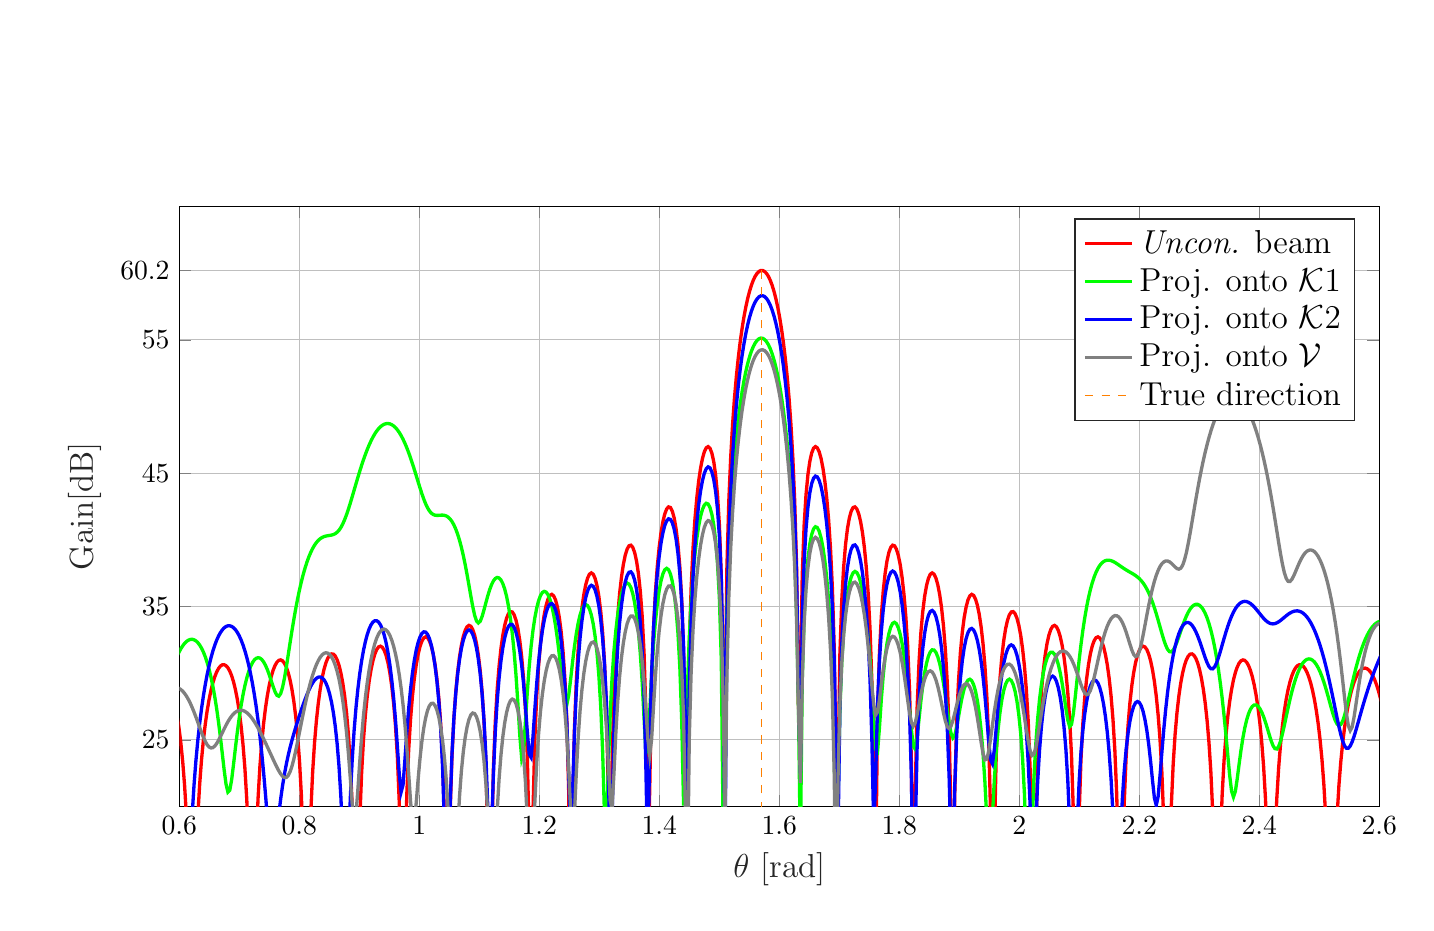
\begin{tikzpicture}

\begin{axis}[%
width=6in,
height=3in,
at={(0.758in,0.481in)},
scale only axis,
xmin=0.6,
xmax=2.6,
xlabel style={font=\large \color{white!15!black}},
xlabel={$\theta~[\mathrm{rad}]$},
ymin=20,
ymax=65,
ytick={ 25, 35, 45, 55, 60.2},
yminorticks=true,
ylabel style={font=\large \color{white!15!black}},
ylabel={Gain[$\mathrm{dB}$]},
xmajorgrids,
ymajorgrids,
axis background/.style={fill=white},
legend style={font = \large , legend cell align=left, align=left, draw=white!15!black}
]
\addplot [color=red, line width=1.2pt]
  table[row sep=crcr]{%
0.0031384541993904	-5.99642473721345\\
0.00627690839878081	-5.59279044739666\\
0.00941536259817121	-4.95915748418816\\
0.0125538167975616	-4.14323746599389\\
0.015692270996952	-3.19563650106894\\
0.0188307251963424	-2.16243734181925\\
0.0219691793957328	-1.0814627861472\\
0.0251076335951232	0.0184993235173993\\
0.0282460877945136	1.11678163471751\\
0.031384541993904	2.19927427748984\\
0.0345229961932944	3.25682329169867\\
0.0376614503926848	4.28385840435167\\
0.0407999045920752	5.27731956706988\\
0.0439383587914656	6.23586044939814\\
0.047076812990856	7.15927656796138\\
0.0502152671902464	8.04810349965607\\
0.0533537213896369	8.90333889422375\\
0.0564921755890272	9.72625248026996\\
0.0596306297884176	10.5182576978164\\
0.0627690839878081	11.2808260819861\\
0.0659075381871985	12.0154311099245\\
0.0690459923865889	12.723512247212\\
0.0721844465859793	13.4064527723371\\
0.0753229007853697	14.0655669424551\\
0.0784613549847601	14.7020934404967\\
0.0815998091841505	15.3171929962536\\
0.0847382633835409	15.9119487329294\\
0.0878767175829313	16.4873682448443\\
0.0910151717823217	17.0443867271398\\
0.0941536259817121	17.5838706959037\\
0.0972920801811025	18.1066219875674\\
0.100430534380493	18.6133818314151\\
0.103568988579883	19.104834859995\\
0.106707442779274	19.5816129731845\\
0.109845896978664	20.0442990046904\\
0.112984351178054	20.4934301637703\\
0.116122805377445	20.9295012399945\\
0.119261259576835	21.3529675696741\\
0.122399713776226	21.7642477690032\\
0.125538167975616	22.1637262431807\\
0.128676622175006	22.5517554832116\\
0.131815076374397	22.9286581631222\\
0.134953530573787	23.2947290508289\\
0.138091984773178	23.6502367457369\\
0.141230438972568	23.9954252554318\\
0.144368893171959	24.3305154234451\\
0.147507347371349	24.6557062188384\\
0.150645801570739	24.9711758977936\\
0.15378425577013	25.2770830461677\\
0.15692270996952	25.5735675112657\\
0.160061164168911	25.8607512300182\\
0.163199618368301	26.1387389599466\\
0.166338072567691	26.4076189184584\\
0.169476526767082	26.6674633351277\\
0.172614980966472	26.9183289208747\\
0.175753435165863	27.1602572572003\\
0.178891889365253	27.3932751077649\\
0.182030343564643	27.6173946540461\\
0.185168797764034	27.8326136557958\\
0.188307251963424	28.038915536516\\
0.191445706162815	28.2362693931334\\
0.194584160362205	28.4246299284066\\
0.197722614561595	28.6039373035381\\
0.200861068760986	28.7741169076904\\
0.203999522960376	28.9350790397812\\
0.207137977159767	29.0867184970219\\
0.210276431359157	29.2289140631176\\
0.213414885558547	29.3615278875989\\
0.216553339757938	29.4844047460709\\
0.219691793957328	29.5973711689518\\
0.222830248156719	29.7002344241094\\
0.225968702356109	29.7927813358385\\
0.229107156555499	29.8747769193435\\
0.23224561075489	29.9459628059495\\
0.23538406495428	30.0060554294603\\
0.238522519153671	30.0547439382996\\
0.241660973353061	30.0916877910874\\
0.244799427552451	30.1165139847333\\
0.247937881751842	30.1288138535385\\
0.251076335951232	30.1281393647675\\
0.254214790150623	30.1139988199147\\
0.257353244350013	30.0858518504113\\
0.260491698549403	30.043103570861\\
0.263630152748794	29.9850977201036\\
0.266768606948184	29.9111085784411\\
0.269907061147575	29.8203313951759\\
0.273045515346965	29.7118709899682\\
0.276183969546355	29.5847280986091\\
0.279322423745746	29.4377829104444\\
0.282460877945136	29.269775079131\\
0.285599332144527	29.0792792634935\\
0.288737786343917	28.8646749464016\\
0.291876240543307	28.6241088491647\\
0.295014694742698	28.355447650884\\
0.298153148942088	28.0562178491134\\
0.301291603141479	27.7235283228569\\
0.304430057340869	27.3539692597344\\
0.307568511540259	26.9434782208952\\
0.31070696573965	26.4871596188056\\
0.31384541993904	25.9790366897154\\
0.316983874138431	25.4117031891893\\
0.320122328337821	24.7758218282262\\
0.323260782537211	24.0593806247779\\
0.326399236736602	23.2465518012006\\
0.329537690935992	22.315867446172\\
0.332676145135383	21.2371534185208\\
0.335814599334773	19.9660451943425\\
0.338953053534163	18.4333618778399\\
0.342091507733554	16.5221918108681\\
0.345229961932944	14.0103708254357\\
0.348368416132335	10.3874055825086\\
0.351506870331725	3.94162169154461\\
0.354645324531115	-11.323735200797\\
0.357783778730506	5.92275912913403\\
0.360922232929896	11.4945859320992\\
0.364060687129287	14.8717420298159\\
0.367199141328677	17.2955651370578\\
0.370337595528067	19.1807945275579\\
0.373476049727458	20.7172530736311\\
0.376614503926848	22.0076991004429\\
0.379752958126239	23.1139855399087\\
0.382891412325629	24.0761768846061\\
0.38602986652502	24.921652784041\\
0.38916832072441	25.6698980869588\\
0.3923067749238	26.3352200631535\\
0.395445229123191	26.9283830924774\\
0.398583683322581	27.4576395274813\\
0.401722137521972	27.9294051964205\\
0.404860591721362	28.3487161951527\\
0.407999045920752	28.7195458128142\\
0.411137500120143	29.0450289488187\\
0.414275954319533	29.3276234410628\\
0.417414408518924	29.569227097261\\
0.420552862718314	29.7712626966834\\
0.423691316917704	29.9347390862001\\
0.426829771117095	30.0602937698159\\
0.429968225316485	30.1482205255195\\
0.433106679515876	30.1984842382001\\
0.436245133715266	30.2107240958602\\
0.439383587914656	30.184245407622\\
0.442522042114047	30.1179994473099\\
0.445660496313437	30.0105497937452\\
0.448798950512828	29.8600225004631\\
0.451937404712218	29.6640359121546\\
0.455075858911608	29.419603796907\\
0.458214313110999	29.1230022733322\\
0.461352767310389	28.7695860934205\\
0.46449122150978	28.353531996311\\
0.46762967570917	27.8674738970717\\
0.47076812990856	27.3019724963247\\
0.473906584107951	26.6447223215835\\
0.477045038307341	25.8793251638697\\
0.480183492506732	24.9833123697418\\
0.483321946706122	23.9247884640811\\
0.486460400905512	22.6563561922435\\
0.489598855104903	21.1031651625186\\
0.492737309304293	19.1366001429187\\
0.495875763503684	16.5061961873126\\
0.499014217703074	12.6117762607636\\
0.502152671902464	5.23745746943484\\
0.505291126101855	-2.27605395956505\\
0.508429580301245	10.132812585697\\
0.511568034500636	15.1205373271876\\
0.514706488700026	18.2551261538248\\
0.517844942899416	20.5276550540469\\
0.520983397098807	22.2950031257659\\
0.524121851298197	23.726357296748\\
0.527260305497588	24.9151554594333\\
0.530398759696978	25.9183051097434\\
0.533537213896368	26.7728871138124\\
0.536675668095759	27.5042627102058\\
0.539814122295149	28.1303961633243\\
0.54295257649454	28.6643285585839\\
0.54609103069393	29.1156726267643\\
0.54922948489332	29.4915543856439\\
0.552367939092711	29.7972244947812\\
0.555506393292101	30.036462353115\\
0.558644847491492	30.211843600711\\
0.561783301690882	30.3249125884796\\
0.564921755890272	30.3762842089006\\
0.568060210089663	30.3656885543981\\
0.571198664289053	30.2919641074452\\
0.574337118488444	30.1529986757642\\
0.577475572687834	29.9456106242078\\
0.580614026887224	29.6653546195524\\
0.583752481086615	29.3062239965242\\
0.586890935286005	28.8602024244746\\
0.590029389485396	28.3165841146346\\
0.593167843684786	27.6609207761652\\
0.596306297884177	26.8733354166647\\
0.599444752083567	25.9256990238806\\
0.602583206282957	24.7766208902219\\
0.605721660482348	23.3618607076904\\
0.608860114681738	21.5740203005118\\
0.611998568881128	19.2129262508794\\
0.615137023080519	15.8347648780968\\
0.618275477279909	10.0721624135129\\
0.6214139314793	-6.70975062072622\\
0.62455238567869	9.6070835367702\\
0.627690839878081	15.6791523928021\\
0.630829294077471	19.1973102645845\\
0.633967748276861	21.6529930066045\\
0.637106202476252	23.5152737594464\\
0.640244656675642	24.9923508305129\\
0.643383110875033	26.1946305275382\\
0.646521565074423	27.1874326053787\\
0.649660019273813	28.0123246779235\\
0.652798473473204	28.6971110711184\\
0.655936927672594	29.2610124682691\\
0.659075381871985	29.7175592848733\\
0.662213836071375	30.0762973342742\\
0.665352290270765	30.3438292699164\\
0.668490744470156	30.5244585503271\\
0.671629198669546	30.6205779252951\\
0.674767652868937	30.6328786598665\\
0.677906107068327	30.560418380068\\
0.681044561267717	30.4005593993334\\
0.684183015467108	30.148767006885\\
0.687321469666498	29.7982315993009\\
0.690459923865889	29.3392412663217\\
0.693598378065279	28.7581679454629\\
0.696736832264669	28.0358104729874\\
0.69987528646406	27.1445925240453\\
0.70301374066345	26.0435668928937\\
0.706152194862841	24.6688329707319\\
0.709290649062231	22.913219330122\\
0.712429103261621	20.5766216217084\\
0.715567557461012	17.2149768548988\\
0.718706011660402	11.4598648133945\\
0.721844465859793	-5.12398039620585\\
0.724982920059183	11.0264333875975\\
0.728121374258573	17.0775303347577\\
0.731259828457964	20.5756173773225\\
0.734398282657354	23.0056670329631\\
0.737536736856745	24.8354537477909\\
0.740675191056135	26.272549279588\\
0.743813645255525	27.4268461392179\\
0.746952099454916	28.3631225645266\\
0.750090553654306	29.1223183760128\\
0.753229007853697	29.7314838291563\\
0.756367462053087	30.2089197235292\\
0.759505916252478	30.5670235246989\\
0.762644370451868	30.8139336359272\\
0.765782824651258	30.9544877241121\\
0.768921278850649	30.990751067265\\
0.772059733050039	30.9222403533078\\
0.775198187249429	30.7458925205633\\
0.77833664144882	30.4557721062578\\
0.78147509564821	30.0424519238957\\
0.784613549847601	29.4919169117992\\
0.787752004046991	28.7836884801428\\
0.790890458246381	27.8875544852635\\
0.794028912445772	26.7575803408492\\
0.797167366645162	25.3202736138411\\
0.800305820844553	23.4485057946483\\
0.803444275043943	20.894130426468\\
0.806582729243334	17.0634200352198\\
0.809721183442724	9.78642418716504\\
0.812859637642114	2.17405552977874\\
0.815998091841505	14.5249513069887\\
0.819136546040895	19.4894642945522\\
0.822275000240286	22.5725079809793\\
0.825413454439676	24.7688173404618\\
0.828551908639066	26.4359569873461\\
0.831690362838457	27.7427457630106\\
0.834828817037847	28.7816956864225\\
0.837967271237237	29.6083554069802\\
0.841105725436628	30.2580181378877\\
0.844244179636018	30.753775101492\\
0.847382633835409	31.1107410234971\\
0.850521088034799	31.3383835602928\\
0.85365954223419	31.441811957609\\
0.85679799643358	31.422424136175\\
0.85993645063297	31.2780905528208\\
0.863074904832361	31.0029228005111\\
0.866213359031751	30.5865670201817\\
0.869351813231142	30.0128260921046\\
0.872490267430532	29.2571777626255\\
0.875628721629922	28.2822589045657\\
0.878767175829313	27.0291972556309\\
0.881905630028703	25.3994257644425\\
0.885044084228094	23.2111317644476\\
0.888182538427484	20.0713684643504\\
0.891320992626874	14.8384847780041\\
0.894459446826265	0.274370022608769\\
0.897597901025655	12.0960085216271\\
0.900736355225046	18.8077258229852\\
0.903874809424436	22.4997724263767\\
0.907013263623826	25.0026910253347\\
0.910151717823217	26.8499005789946\\
0.913290172022607	28.2698292551461\\
0.916428626221997	29.3806059569519\\
0.919567080421388	30.2504217136227\\
0.922705534620778	30.9213146045865\\
0.925843988820169	31.4200518144444\\
0.928982443019559	31.7636127965951\\
0.93212089721895	31.9621001507499\\
0.93525935141834	32.0202698941889\\
0.93839780561773	31.9382084308935\\
0.941536259817121	31.7113654101802\\
0.944674714016511	31.3299525543428\\
0.947813168215902	30.7775248578319\\
0.950951622415292	30.0282635735338\\
0.954090076614682	29.0418740116665\\
0.957228530814073	27.7535430611645\\
0.960366985013463	26.0522748276261\\
0.963505439212854	23.7269952979944\\
0.966643893412244	20.298366059948\\
0.969782347611634	14.219145259356\\
0.972920801811025	-2.20101666629497\\
0.976059256010415	15.1714923127127\\
0.979197710209806	20.8867105885086\\
0.982336164409196	24.2368076686069\\
0.985474618608586	26.5551610071732\\
0.988613072807977	28.2763520938451\\
0.991751527007367	29.5958321353501\\
0.994889981206758	30.6172981696937\\
0.998028435406148	31.4012970698969\\
1.00116688960554	31.9850784686539\\
1.00430534380493	32.3918594837653\\
1.00744379800432	32.6355022884974\\
1.01058225220371	32.72291732592\\
1.0137207064031	32.6551613279512\\
1.01685916060249	32.4276172610672\\
1.01999761480188	32.029316373601\\
1.02313606900127	31.4411722009835\\
1.02627452320066	30.6324614170876\\
1.02941297740005	29.5539720481459\\
1.03255143159944	28.1239031279139\\
1.03568988579883	26.1955178596638\\
1.03882833999822	23.4688744330468\\
1.04196679419761	19.1677488882772\\
1.045105248397	9.78957218204447\\
1.04824370259639	10.3187773529512\\
1.05138215679578	19.4701448803219\\
1.05452061099518	23.7906287627366\\
1.05765906519457	26.5735719521642\\
1.06079751939396	28.5690351379741\\
1.06393597359335	30.0691910029995\\
1.06707442779274	31.2172422023329\\
1.07021288199213	32.0927823080268\\
1.07335133619152	32.7432451539382\\
1.07648979039091	33.1976247700772\\
1.0796282445903	33.4730960932381\\
1.08276669878969	33.578324897076\\
1.08590515298908	33.5149746931862\\
1.08904360718847	33.2780001117058\\
1.09218206138786	32.8548342134291\\
1.09532051558725	32.2231674593306\\
1.09845896978664	31.3463968897479\\
1.10159742398603	30.164466259761\\
1.10473587818542	28.5741347215628\\
1.10787433238481	26.3805931370699\\
1.1110127865842	23.1506465744851\\
1.11415124078359	17.5536306890568\\
1.11728969498298	-0.939044300589249\\
1.12042814918237	16.6532628702645\\
1.12356660338176	22.8664043483735\\
1.12670505758115	26.3786015773713\\
1.12984351178054	28.7682443099258\\
1.13298196597994	30.5186534164586\\
1.13612042017933	31.8410123147082\\
1.13925887437872	32.8451627503388\\
1.14239732857811	33.5939983589673\\
1.1455357827775	34.1251687856398\\
1.14867423697689	34.460978434897\\
1.15181269117628	34.6131979514573\\
1.15495114537567	34.585299568483\\
1.15808959957506	34.3730894561285\\
1.16122805377445	33.963988147863\\
1.16436650797384	33.3346733538012\\
1.16750496217323	32.4460509041734\\
1.17064341637262	31.2328933364674\\
1.17378187057201	29.5809797539565\\
1.1769203247714	27.2691749573679\\
1.18005877897079	23.7840275080282\\
1.18319723317018	17.3866159470385\\
1.18633568736957	2.23246610609685\\
1.18947414156896	19.5563217561513\\
1.19261259576835	25.044703640786\\
1.19575104996774	28.2999656112989\\
1.19888950416713	30.5514646359984\\
1.20202795836652	32.209238747032\\
1.20516641256591	33.4593104028549\\
1.20830486676531	34.4002473624819\\
1.2114433209647	35.088789183132\\
1.21458177516409	35.5585408404854\\
1.21772022936348	35.8285767726603\\
1.22085868356287	35.9075362913161\\
1.22399713776226	35.7953007638793\\
1.22713559196165	35.4829893718659\\
1.23027404616104	34.9512720537388\\
1.23341250036043	34.1662589171234\\
1.23655095455982	33.0708668126739\\
1.23968940875921	31.566055666466\\
1.2428278629586	29.4649916586895\\
1.24596631715799	26.3556147737461\\
1.24910477135738	20.9987918265153\\
1.25224322555677	3.18347585807228\\
1.25538167975616	19.1677389126804\\
1.25852013395555	25.7017415180474\\
1.26165858815494	29.3210585500119\\
1.26479704235433	31.7640085201338\\
1.26793549655372	33.5427112332752\\
1.27107395075311	34.8771759023327\\
1.2742124049525	35.8804463429662\\
1.27735085915189	36.6163683076682\\
1.28048931335128	37.1223112595796\\
1.28362776755067	37.4193546480614\\
1.28676622175007	37.517057189851\\
1.28990467594946	37.415396841456\\
1.29304313014885	37.104779572879\\
1.29618158434824	36.5641211061776\\
1.29932003854763	35.7561151910564\\
1.30245849274702	34.6171270827446\\
1.30559694694641	33.0346703569096\\
1.3087354011458	30.7902354286869\\
1.31187385534519	27.3765132067596\\
1.31501230954458	21.079226881473\\
1.31815076374397	3.97958276234809\\
1.32128921794336	23.0808894835216\\
1.32442767214275	28.6673183957377\\
1.32756612634214	31.9714916695417\\
1.33070458054153	34.2558661367544\\
1.33384303474092	35.9368286263759\\
1.33698148894031	37.2021528771398\\
1.3401199431397	38.1506969741513\\
1.34325839733909	38.8387553427442\\
1.34639685153848	39.2989131909547\\
1.34953530573787	39.5485946476929\\
1.35267375993726	39.5939443997073\\
1.35581221413665	39.4310861297623\\
1.35895066833604	39.0453428816137\\
1.36208912253543	38.408061886562\\
1.36522757673483	37.4694344671798\\
1.36836603093422	36.1428489611712\\
1.37150448513361	34.2676388341318\\
1.374642939333	31.5029935858803\\
1.37778139353239	26.9091533706949\\
1.38091984773178	15.1457493462071\\
1.38405830193117	21.2447193562665\\
1.38719675613056	29.2412399561374\\
1.39033521032995	33.3149633850734\\
1.39347366452934	36.0051339281156\\
1.39661211872873	37.952769560116\\
1.39975057292812	39.417307503955\\
1.40288902712751	40.5277768033799\\
1.4060274813269	41.3555618436253\\
1.40916593552629	41.9418196250381\\
1.41230438972568	42.3094201189637\\
1.41544284392507	42.4684023409788\\
1.41858129812446	42.4181018950932\\
1.42171975232385	42.1469964024216\\
1.42485820652324	41.6301964009203\\
1.42799666072263	40.8233265848772\\
1.43113511492202	39.6491430549765\\
1.43427356912141	37.9663278965806\\
1.4374120233208	35.4842196715461\\
1.44055047752019	31.452028270216\\
1.44368893171959	22.4774047759838\\
1.44682738591898	21.8615361092675\\
1.44996584011837	31.8235226841921\\
1.45310429431776	36.4009934425059\\
1.45624274851715	39.3658193693887\\
1.45938120271654	41.5115798989144\\
1.46251965691593	43.1409127463643\\
1.46565811111532	44.3999905847928\\
1.46879656531471	45.368528675793\\
1.4719350195141	46.0923758667925\\
1.47507347371349	46.5973936665219\\
1.47821192791288	46.8957636153592\\
1.48135038211227	46.988544432933\\
1.48448883631166	46.8657743077395\\
1.48762729051105	46.5041633422756\\
1.49076574471044	45.8612109884595\\
1.49390419890983	44.86224062049\\
1.49704265310922	43.3702086690398\\
1.50018110730861	41.1037240394306\\
1.503319561508	37.3420909548975\\
1.50645801570739	28.9298569972887\\
1.50959646990678	27.2912922647064\\
1.51273492410617	37.9651007409201\\
1.51587337830556	42.8850563928396\\
1.51901183250496	46.1633325412505\\
1.52215028670435	48.6307920715399\\
1.52528874090374	50.6030121801656\\
1.52842719510313	52.2343531556686\\
1.53156564930252	53.6120095421643\\
1.53470410350191	54.7900811865057\\
1.5378425577013	55.8044155237558\\
1.54098101190069	56.6799324749848\\
1.54411946610008	57.4345825056953\\
1.54725792029947	58.0816378686069\\
1.55039637449886	58.6310920681425\\
1.55353482869825	59.0905514016513\\
1.55667328289764	59.4658216359222\\
1.55981173709703	59.7613030871914\\
1.56295019129642	59.9802600090412\\
1.56608864549581	60.1250038520518\\
1.5692270996952	60.1970145589734\\
1.57236555389459	60.1970145589734\\
1.57550400809398	60.1250038520518\\
1.57864246229337	59.9802600090412\\
1.58178091649276	59.7613030871914\\
1.58491937069215	59.4658216359222\\
1.58805782489154	59.0905514016513\\
1.59119627909093	58.6310920681424\\
1.59433473329032	58.0816378686068\\
1.59747318748972	57.4345825056953\\
1.60061164168911	56.6799324749848\\
1.6037500958885	55.8044155237559\\
1.60688855008789	54.7900811865057\\
1.61002700428728	53.6120095421641\\
1.61316545848667	52.2343531556686\\
1.61630391268606	50.6030121801656\\
1.61944236688545	48.6307920715399\\
1.62258082108484	46.1633325412502\\
1.62571927528423	42.8850563928398\\
1.62885772948362	37.9651007409195\\
1.63199618368301	27.2912922647074\\
1.6351346378824	28.9298569972888\\
1.63827309208179	37.3420909548972\\
1.64141154628118	41.1037240394306\\
1.64455000048057	43.3702086690398\\
1.64768845467996	44.8622406204899\\
1.65082690887935	45.8612109884596\\
1.65396536307874	46.5041633422755\\
1.65710381727813	46.8657743077394\\
1.66024227147752	46.9885444329329\\
1.66338072567691	46.8957636153593\\
1.6665191798763	46.5973936665218\\
1.66965763407569	46.0923758667927\\
1.67279608827508	45.368528675793\\
1.67593454247447	44.3999905847928\\
1.67907299667387	43.1409127463645\\
1.68221145087326	41.5115798989142\\
1.68534990507265	39.3658193693885\\
1.68848835927204	36.4009934425061\\
1.69162681347143	31.823522684192\\
1.69476526767082	21.8615361092671\\
1.69790372187021	22.4774047759863\\
1.7010421760696	31.4520282702167\\
1.70418063026899	35.4842196715466\\
1.70731908446838	37.9663278965805\\
1.71045753866777	39.6491430549762\\
1.71359599286716	40.8233265848775\\
1.71673444706655	41.6301964009204\\
1.71987290126594	42.1469964024218\\
1.72301135546533	42.4181018950932\\
1.72614980966472	42.4684023409789\\
1.72928826386411	42.3094201189637\\
1.7324267180635	41.9418196250381\\
1.73556517226289	41.3555618436253\\
1.73870362646228	40.52777680338\\
1.74184208066167	39.4173075039547\\
1.74498053486106	37.9527695601154\\
1.74811898906045	36.0051339281155\\
1.75125744325984	33.3149633850736\\
1.75439589745924	29.2412399561374\\
1.75753435165863	21.2447193562666\\
1.76067280585802	15.1457493462072\\
1.76381126005741	26.9091533706949\\
1.7669497142568	31.5029935858803\\
1.77008816845619	34.2676388341318\\
1.77322662265558	36.1428489611705\\
1.77636507685497	37.4694344671804\\
1.77950353105436	38.408061886562\\
1.78264198525375	39.0453428816137\\
1.78578043945314	39.4310861297623\\
1.78891889365253	39.5939443997075\\
1.79205734785192	39.5485946476927\\
1.79519580205131	39.2989131909547\\
1.7983342562507	38.8387553427442\\
1.80147271045009	38.1506969741516\\
1.80461116464948	37.2021528771396\\
1.80774961884887	35.9368286263759\\
1.81088807304826	34.2558661367545\\
1.81402652724765	31.9714916695417\\
1.81716498144704	28.6673183957377\\
1.82030343564643	23.0808894835223\\
1.82344188984582	3.97958276235981\\
1.82658034404521	21.0792268814735\\
1.8297187982446	27.3765132067593\\
1.83285725244399	30.7902354286866\\
1.83599570664339	33.0346703569094\\
1.83913416084278	34.6171270827443\\
1.84227261504217	35.7561151910561\\
1.84541106924156	36.5641211061777\\
1.84854952344095	37.1047795728788\\
1.85168797764034	37.4153968414559\\
1.85482643183973	37.517057189851\\
1.85796488603912	37.4193546480611\\
1.86110334023851	37.1223112595802\\
1.8642417944379	36.6163683076675\\
1.86738024863729	35.8804463429669\\
1.87051870283668	34.8771759023328\\
1.87365715703607	33.5427112332751\\
1.87679561123546	31.7640085201348\\
1.87993406543485	29.321058550013\\
1.88307251963424	25.7017415180481\\
1.88621097383363	19.167738912678\\
1.88934942803302	3.18347585807074\\
1.89248788223241	20.9987918265142\\
1.8956263364318	26.3556147737466\\
1.89876479063119	29.4649916586884\\
1.90190324483058	31.5660556664659\\
1.90504169902997	33.0708668126739\\
1.90818015322936	34.1662589171232\\
1.91131860742876	34.9512720537389\\
1.91445706162815	35.482989371865\\
1.91759551582754	35.795300763879\\
1.92073397002693	35.9075362913159\\
1.92387242422632	35.8285767726602\\
1.92701087842571	35.5585408404855\\
1.9301493326251	35.0887891831322\\
1.93328778682449	34.4002473624822\\
1.93642624102388	33.4593104028549\\
1.93956469522327	32.209238747032\\
1.94270314942266	30.5514646359982\\
1.94584160362205	28.2999656112985\\
1.94898005782144	25.0447036407854\\
1.95211851202083	19.5563217561535\\
1.95525696622022	2.23246610609551\\
1.95839542041961	17.3866159470378\\
1.961533874619	23.7840275080259\\
1.96467232881839	27.2691749573674\\
1.96781078301778	29.5809797539548\\
1.97094923721717	31.2328933364672\\
1.97408769141656	32.4460509041735\\
1.97722614561595	33.3346733538022\\
1.98036459981534	33.9639881478635\\
1.98350305401473	34.3730894561285\\
1.98664150821412	34.5852995684829\\
1.98977996241352	34.6131979514575\\
1.99291841661291	34.460978434897\\
1.9960568708123	34.1251687856398\\
1.99919532501169	33.5939983589671\\
2.00233377921108	32.8451627503385\\
2.00547223341047	31.8410123147083\\
2.00861068760986	30.5186534164591\\
2.01174914180925	28.7682443099258\\
2.01488759600864	26.3786015773691\\
2.01802605020803	22.8664043483766\\
2.02116450440742	16.6532628702715\\
2.02430295860681	-0.939044300609283\\
2.0274414128062	17.5536306890563\\
2.03057986700559	23.150646574486\\
2.03371832120498	26.3805931370706\\
2.03685677540437	28.5741347215627\\
2.03999522960376	30.1644662597596\\
2.04313368380315	31.3463968897477\\
2.04627213800254	32.2231674593312\\
2.04941059220193	32.8548342134288\\
2.05254904640132	33.2780001117057\\
2.05568750060071	33.5149746931861\\
2.0588259548001	33.5783248970762\\
2.06196440899949	33.4730960932379\\
2.06510286319888	33.197624770077\\
2.06824131739828	32.7432451539379\\
2.07137977159767	32.0927823080273\\
2.07451822579706	31.2172422023325\\
2.07765667999645	30.0691910029987\\
2.08079513419584	28.5690351379751\\
2.08393358839523	26.5735719521646\\
2.08707204259462	23.790628762733\\
2.09021049679401	19.4701448803253\\
2.0933489509934	10.3187773529475\\
2.09648740519279	9.78957218204449\\
2.09962585939218	19.1677488882772\\
2.10276431359157	23.4688744330477\\
2.10590276779096	26.1955178596633\\
2.10904122199035	28.1239031279139\\
2.11217967618974	29.5539720481464\\
2.11531813038913	30.6324614170874\\
2.11845658458852	31.4411722009841\\
2.12159503878791	32.0293163736016\\
2.1247334929873	32.4276172610672\\
2.12787194718669	32.6551613279518\\
2.13101040138608	32.7229173259201\\
2.13414885558547	32.6355022884974\\
2.13728730978486	32.3918594837655\\
2.14042576398425	31.9850784686538\\
2.14356421818364	31.4012970698967\\
2.14670267238304	30.6172981696937\\
2.14984112658243	29.5958321353501\\
2.15297958078182	28.2763520938424\\
2.15611803498121	26.5551610071742\\
2.1592564891806	24.236807668608\\
2.16239494337999	20.8867105885092\\
2.16553339757938	15.1714923127132\\
2.16867185177877	-2.20101666629538\\
2.17181030597816	14.219145259355\\
2.17494876017755	20.2983660599495\\
2.17808721437694	23.7269952979946\\
2.18122566857633	26.0522748276273\\
2.18436412277572	27.7535430611646\\
2.18750257697511	29.0418740116662\\
2.1906410311745	30.0282635735337\\
2.19377948537389	30.7775248578327\\
2.19691793957328	31.3299525543425\\
2.20005639377267	31.7113654101804\\
2.20319484797206	31.9382084308944\\
2.20633330217145	32.0202698941888\\
2.20947175637084	31.9621001507495\\
2.21261021057023	31.7636127965956\\
2.21574866476962	31.4200518144453\\
2.21888711896901	30.9213146045865\\
2.22202557316841	30.2504217136228\\
2.2251640273678	29.3806059569523\\
2.22830248156719	28.2698292551455\\
2.23144093576658	26.8499005789954\\
2.23457938996597	25.0026910253345\\
2.23771784416536	22.499772426375\\
2.24085629836475	18.8077258229839\\
2.24399475256414	12.0960085216342\\
2.24713320676353	0.274370022597165\\
2.25027166096292	14.8384847780051\\
2.25341011516231	20.071368464352\\
2.2565485693617	23.2111317644491\\
2.25968702356109	25.3994257644426\\
2.26282547776048	27.0291972556307\\
2.26596393195987	28.2822589045656\\
2.26910238615926	29.2571777626256\\
2.27224084035865	30.0128260921042\\
2.27537929455804	30.5865670201817\\
2.27851774875743	31.0029228005111\\
2.28165620295682	31.2780905528208\\
2.28479465715621	31.4224241361749\\
2.2879331113556	31.441811957609\\
2.29107156555499	31.3383835602927\\
2.29421001975438	31.1107410234976\\
2.29734847395377	30.7537751014913\\
2.30048692815316	30.258018137889\\
2.30362538235256	29.6083554069812\\
2.30676383655195	28.7816956864224\\
2.30990229075134	27.7427457630106\\
2.31304074495073	26.435956987346\\
2.31617919915012	24.7688173404624\\
2.31931765334951	22.57250798098\\
2.3224561075489	19.4894642945517\\
2.32559456174829	14.5249513069868\\
2.32873301594768	2.17405552979971\\
2.33187147014707	9.78642418716181\\
2.33500992434646	17.0634200352129\\
2.33814837854585	20.894130426467\\
2.34128683274524	23.4485057946485\\
2.34442528694463	25.3202736138414\\
2.34756374114402	26.7575803408492\\
2.35070219534341	27.8875544852636\\
2.3538406495428	28.7836884801427\\
2.35697910374219	29.4919169117991\\
2.36011755794158	30.0424519238957\\
2.36325601214097	30.4557721062575\\
2.36639446634036	30.7458925205639\\
2.36953292053975	30.9222403533071\\
2.37267137473914	30.9907510672651\\
2.37580982893853	30.9544877241124\\
2.37894828313792	30.813933635926\\
2.38208673733732	30.5670235246989\\
2.38522519153671	30.2089197235283\\
2.3883636457361	29.7314838291563\\
2.39150209993549	29.1223183760122\\
2.39464055413488	28.3631225645261\\
2.39777900833427	27.4268461392184\\
2.40091746253366	26.2725492795876\\
2.40405591673305	24.8354537477918\\
2.40719437093244	23.0056670329637\\
2.41033282513183	20.5756173773155\\
2.41347127933122	17.0775303347546\\
2.41660973353061	11.0264333875839\\
2.41974818773	-5.12398039618781\\
2.42288664192939	11.459864813396\\
2.42602509612878	17.2149768548937\\
2.42916355032817	20.5766216217069\\
2.43230200452756	22.9132193301233\\
2.43544045872695	24.6688329707321\\
2.43857891292634	26.043566892894\\
2.44171736712573	27.144592524045\\
2.44485582132512	28.0358104729871\\
2.44799427552451	28.7581679454622\\
2.4511327297239	29.3392412663215\\
2.4542711839233	29.7982315993006\\
2.45740963812269	30.1487670068855\\
2.46054809232208	30.4005593993339\\
2.46368654652147	30.5604183800682\\
2.46682500072086	30.6328786598664\\
2.46996345492025	30.6205779252952\\
2.47310190911964	30.5244585503274\\
2.47624036331903	30.3438292699175\\
2.47937881751842	30.0762973342745\\
2.48251727171781	29.7175592848733\\
2.4856557259172	29.261012468269\\
2.48879418011659	28.69711107112\\
2.49193263431598	28.0123246779228\\
2.49507108851537	27.1874326053765\\
2.49820954271476	26.1946305275381\\
2.50134799691415	24.9923508305122\\
2.50448645111354	23.5152737594448\\
2.50762490531293	21.6529930066028\\
2.51076335951232	19.1973102645836\\
2.51390181371171	15.6791523928025\\
2.5170402679111	9.60708353676999\\
2.52017872211049	-6.70975062072361\\
2.52331717630988	10.0721624135092\\
2.52645563050927	15.834764878097\\
2.52959408470866	19.2129262508784\\
2.53273253890806	21.5740203005118\\
2.53587099310745	23.3618607076904\\
2.53900944730684	24.7766208902216\\
2.54214790150623	25.9256990238808\\
2.54528635570562	26.8733354166646\\
2.54842480990501	27.660920776166\\
2.5515632641044	28.3165841146338\\
2.55470171830379	28.8602024244744\\
2.55784017250318	29.3062239965245\\
2.56097862670257	29.6653546195522\\
2.56411708090196	29.9456106242071\\
2.56725553510135	30.1529986757642\\
2.57039398930074	30.291964107445\\
2.57353244350013	30.3656885543989\\
2.57667089769952	30.376284208901\\
2.57980935189891	30.3249125884798\\
2.5829478060983	30.2118436007104\\
2.58608626029769	30.0364623531147\\
2.58922471449708	29.7972244947826\\
2.59236316869647	29.4915543856435\\
2.59550162289586	29.1156726267644\\
2.59864007709525	28.6643285585842\\
2.60177853129464	28.1303961633236\\
2.60491698549403	27.5042627102062\\
2.60805543969342	26.7728871138126\\
2.61119389389282	25.918305109743\\
2.61433234809221	24.9151554594333\\
2.6174708022916	23.7263572967485\\
2.62060925649099	22.2950031257663\\
2.62374771069038	20.5276550540437\\
2.62688616488977	18.2551261538254\\
2.63002461908916	15.120537327186\\
2.63316307328855	10.1328125857059\\
2.63630152748794	-2.27605395956192\\
2.63943998168733	5.23745746945069\\
2.64257843588672	12.6117762607653\\
2.64571689008611	16.5061961873147\\
2.6488553442855	19.1366001429193\\
2.65199379848489	21.1031651625219\\
2.65513225268428	22.656356192242\\
2.65827070688367	23.9247884640818\\
2.66140916108306	24.9833123697418\\
2.66454761528245	25.8793251638708\\
2.66768606948184	26.6447223215837\\
2.67082452368123	27.3019724963248\\
2.67396297788062	27.8674738970711\\
2.67710143208001	28.3535319963121\\
2.6802398862794	28.7695860934211\\
2.68337834047879	29.1230022733322\\
2.68651679467818	29.419603796907\\
2.68965524887758	29.6640359121522\\
2.69279370307697	29.8600225004626\\
2.69593215727636	30.0105497937452\\
2.69907061147575	30.1179994473096\\
2.70220906567514	30.1842454076215\\
2.70534751987453	30.2107240958594\\
2.70848597407392	30.1984842381997\\
2.71162442827331	30.1482205255199\\
2.7147628824727	30.0602937698151\\
2.71790133667209	29.9347390861999\\
2.72103979087148	29.7712626966832\\
2.72417824507087	29.5692270972602\\
2.72731669927026	29.3276234410628\\
2.73045515346965	29.0450289488185\\
2.73359360766904	28.7195458128137\\
2.73673206186843	28.3487161951522\\
2.73987051606782	27.9294051964195\\
2.74300897026721	27.4576395274812\\
2.7461474244666	26.9283830924767\\
2.74928587866599	26.3352200631527\\
2.75242433286538	25.6698980869585\\
2.75556278706477	24.921652784039\\
2.75870124126416	24.0761768846045\\
2.76183969546355	23.1139855399092\\
2.76497814966294	22.0076991004406\\
2.76811660386234	20.7172530736326\\
2.77125505806173	19.1807945275577\\
2.77439351226112	17.2955651370532\\
2.77753196646051	14.8717420298125\\
2.7806704206599	11.4945859320987\\
2.78380887485929	5.92275912912749\\
2.78694732905868	-11.3237352006504\\
2.79008578325807	3.94162169154872\\
2.79322423745746	10.3874055825055\\
2.79636269165685	14.0103708254397\\
2.79950114585624	16.5221918108691\\
2.80263960005563	18.4333618778402\\
2.80577805425502	19.9660451943448\\
2.80891650845441	21.2371534185201\\
2.8120549626538	22.315867446173\\
2.81519341685319	23.2465518012011\\
2.81833187105258	24.0593806247786\\
2.82147032525197	24.7758218282263\\
2.82460877945136	25.4117031891903\\
2.82774723365075	25.9790366897154\\
2.83088568785014	26.487159618805\\
2.83402414204953	26.9434782208956\\
2.83716259624892	27.3539692597334\\
2.84030105044831	27.7235283228573\\
2.84343950464771	28.0562178491136\\
2.8465779588471	28.3554476508844\\
2.84971641304649	28.6241088491648\\
2.85285486724588	28.8646749464021\\
2.85599332144527	29.0792792634933\\
2.85913177564466	29.2697750791312\\
2.86227022984405	29.4377829104445\\
2.86540868404344	29.5847280986102\\
2.86854713824283	29.7118709899685\\
2.87168559244222	29.8203313951763\\
2.87482404664161	29.9111085784421\\
2.877962500841	29.9850977201037\\
2.88110095504039	30.0431035708625\\
2.88423940923978	30.0858518504117\\
2.88737786343917	30.1139988199152\\
2.89051631763856	30.1281393647678\\
2.89365477183795	30.128813853539\\
2.89679322603734	30.1165139847335\\
2.89993168023673	30.0916877910875\\
2.90307013443612	30.0547439383004\\
2.90620858863551	30.0060554294624\\
2.9093470428349	29.9459628059492\\
2.91248549703429	29.8747769193436\\
2.91562395123368	29.7927813358387\\
2.91876240543307	29.7002344241098\\
2.92190085963247	29.5973711689522\\
2.92503931383186	29.4844047460717\\
2.92817776803125	29.3615278875995\\
2.93131622223064	29.2289140631185\\
2.93445467643003	29.0867184970233\\
2.93759313062942	28.9350790397807\\
2.94073158482881	28.7741169076909\\
2.9438700390282	28.6039373035382\\
2.94700849322759	28.4246299284062\\
2.95014694742698	28.2362693931364\\
2.95328540162637	28.0389155365156\\
2.95642385582576	27.8326136557964\\
2.95956231002515	27.6173946540462\\
2.96270076422454	27.3932751077685\\
2.96583921842393	27.1602572572007\\
2.96897767262332	26.918328920876\\
2.97211612682271	26.6674633351276\\
2.9752545810221	26.4076189184595\\
2.97839303522149	26.1387389599473\\
2.98153148942088	25.8607512300169\\
2.98466994362027	25.5735675112663\\
2.98780839781966	25.2770830461687\\
2.99094685201905	24.971175897793\\
2.99408530621844	24.6557062188392\\
2.99722376041783	24.3305154234457\\
3.00036221461722	23.9954252554349\\
3.00350066881662	23.6502367457379\\
3.00663912301601	23.2947290508271\\
3.0097775772154	22.9286581631221\\
3.01291603141479	22.551755483211\\
3.01605448561418	22.1637262431793\\
3.01919293981357	21.7642477690052\\
3.02233139401296	21.3529675696743\\
3.02546984821235	20.9295012399986\\
3.02860830241174	20.4934301637702\\
3.03174675661113	20.0442990046901\\
3.03488521081052	19.5816129731872\\
3.03802366500991	19.1048348599983\\
3.0411621192093	18.6133818314156\\
3.04430057340869	18.1066219875681\\
3.04743902760808	17.5838706959042\\
3.05057748180747	17.0443867271411\\
3.05371593600686	16.4873682448503\\
3.05685439020625	15.9119487329306\\
3.05999284440564	15.3171929962516\\
3.06313129860503	14.702093440502\\
3.06626975280442	14.0655669424529\\
3.06940820700381	13.4064527723365\\
3.0725466612032	12.7235122472142\\
3.07568511540259	12.0154311099275\\
3.07882356960198	11.2808260819789\\
3.08196202380138	10.5182576978154\\
3.08510047800077	9.72625248027149\\
3.08823893220016	8.90333889422046\\
3.09137738639955	8.04810349965129\\
3.09451584059894	7.15927656795838\\
3.09765429479833	6.23586044939264\\
3.10079274899772	5.27731956707846\\
3.10393120319711	4.2838584043466\\
3.1070696573965	3.25682329169262\\
3.11020811159589	2.19927427749555\\
3.11334656579528	1.11678163471759\\
3.11648501999467	0.0184993235256842\\
3.11962347419406	-1.08146278616598\\
3.12276192839345	-2.16243734182967\\
3.12590038259284	-3.19563650105281\\
3.12903883679223	-4.14323746598748\\
3.13217729099162	-4.95915748416796\\
3.13531574519101	-5.59279044744455\\
3.1384541993904	-5.99642473722975\\
};
\addlegendentry{\emph{Uncon.} beam}

\addplot [color=green, line width=1.2pt]
  table[row sep=crcr]{%
0.0031384541993904	30.4362311869824\\
0.00627690839878081	30.434102661184\\
0.00941536259817121	30.4305451705098\\
0.0125538167975616	30.4255437789416\\
0.015692270996952	30.4190775468783\\
0.0188307251963424	30.4111195015628\\
0.0219691793957328	30.401636598467\\
0.0251076335951232	30.3905896732265\\
0.0282460877945136	30.3779333835472\\
0.031384541993904	30.363616140462\\
0.0345229961932944	30.347580028128\\
0.0376614503926848	30.3297607113299\\
0.0407999045920752	30.3100873296252\\
0.0439383587914656	30.288482376985\\
0.047076812990856	30.2648615656562\\
0.0502152671902464	30.239133672746\\
0.0533537213896369	30.2112003678975\\
0.0564921755890272	30.1809560202515\\
0.0596306297884176	30.1482874826241\\
0.0627690839878081	30.1130738506542\\
0.0659075381871985	30.0751861943956\\
0.0690459923865889	30.0344872595476\\
0.0721844465859793	29.9908311352232\\
0.0753229007853697	29.9440628847743\\
0.0784613549847601	29.8940181358614\\
0.0815998091841505	29.8405226254764\\
0.0847382633835409	29.7833916951632\\
0.0878767175829313	29.7224297311941\\
0.0910151717823217	29.6574295437944\\
0.0941536259817121	29.5881716789425\\
0.0972920801811025	29.5144236554992\\
0.100430534380493	29.4359391196287\\
0.103568988579883	29.3524569076993\\
0.106707442779274	29.2637000078414\\
0.109845896978664	29.1693744094501\\
0.112984351178054	29.0691678288676\\
0.116122805377445	28.9627482985708\\
0.119261259576835	28.8497626061902\\
0.122399713776226	28.7298345690246\\
0.125538167975616	28.602563129196\\
0.128676622175006	28.467520254756\\
0.131815076374397	28.3242486329301\\
0.134953530573787	28.1722591440562\\
0.138091984773178	28.0110281090296\\
0.141230438972568	27.8399943107077\\
0.144368893171959	27.6585558018296\\
0.147507347371349	27.4660665314808\\
0.150645801570739	27.2618328520534\\
0.15378425577013	27.0451100145745\\
0.15692270996952	26.8150988299658\\
0.160061164168911	26.5709427791685\\
0.163199618368301	26.3117260138912\\
0.166338072567691	26.0364729292246\\
0.169476526767082	25.7441503503827\\
0.172614980966472	25.4336739204674\\
0.175753435165863	25.1039210985496\\
0.178891889365253	24.7537544188337\\
0.182030343564643	24.3820605319346\\
0.185168797764034	23.9878133527278\\
0.188307251963424	23.5701737953246\\
0.191445706162815	23.1286446141718\\
0.194584160362205	22.663307317985\\
0.197722614561595	22.1751791184622\\
0.200861068760986	21.6667401005275\\
0.203999522960376	21.1426889694374\\
0.207137977159767	20.6109754571455\\
0.210276431359157	20.0840969653914\\
0.213414885558547	19.5804802258901\\
0.216553339757938	19.1254319592266\\
0.219691793957328	18.7506579730822\\
0.222830248156719	18.4910397528229\\
0.225968702356109	18.3779842289804\\
0.229107156555499	18.4308300014413\\
0.23224561075489	18.6503741437785\\
0.23538406495428	19.0185471145517\\
0.238522519153671	19.5044553195027\\
0.241660973353061	20.0729776078262\\
0.244799427552451	20.6916986594118\\
0.247937881751842	21.3344390275068\\
0.251076335951232	21.9819323413126\\
0.254214790150623	22.6209562408839\\
0.257353244350013	23.2429618029739\\
0.260491698549403	23.8427576247872\\
0.263630152748794	24.4174508143296\\
0.266768606948184	24.965667133517\\
0.269907061147575	25.4870049965537\\
0.273045515346965	25.9816648131411\\
0.276183969546355	26.450202438315\\
0.279322423745746	26.8933676545913\\
0.282460877945136	27.3119998101067\\
0.285599332144527	27.7069614231583\\
0.288737786343917	28.0790968018183\\
0.291876240543307	28.4292070322935\\
0.295014694742698	28.7580355969545\\
0.298153148942088	29.0662608237368\\
0.301291603141479	29.3544926569758\\
0.304430057340869	29.6232720925963\\
0.307568511540259	29.8730721852913\\
0.31070696573965	30.1042999085766\\
0.31384541993904	30.3172983957906\\
0.316983874138431	30.5123492532142\\
0.320122328337821	30.6896747435556\\
0.323260782537211	30.8494397079602\\
0.326399236736602	30.9917531392192\\
0.329537690935992	31.1166693463323\\
0.332676145135383	31.2241886663988\\
0.335814599334773	31.3142576871407\\
0.338953053534163	31.3867689449092\\
0.342091507733554	31.4415600597591\\
0.345229961932944	31.4784122622307\\
0.348368416132335	31.4970482559565\\
0.351506870331725	31.4971293462076\\
0.354645324531115	31.4782517467527\\
0.357783778730506	31.4399419551249\\
0.360922232929896	31.3816510588438\\
0.364060687129287	31.3027478009503\\
0.367199141328677	31.2025101907002\\
0.370337595528067	31.0801153921287\\
0.373476049727458	30.9346275568242\\
0.376614503926848	30.7649831837231\\
0.379752958126239	30.5699734838142\\
0.382891412325629	30.3482230958796\\
0.38602986652502	30.0981643346168\\
0.38916832072441	29.8180059488838\\
0.3923067749238	29.5056951212125\\
0.395445229123191	29.1588711532004\\
0.398583683322581	28.7748089753283\\
0.401722137521972	28.3503503556055\\
0.404860591721362	27.8818206139348\\
0.407999045920752	27.3649291389901\\
0.411137500120143	26.7946538735451\\
0.414275954319533	26.1651150369386\\
0.417414408518924	25.4694558974717\\
0.420552862718314	24.699778040669\\
0.423691316917704	23.8472477046476\\
0.426829771117095	22.9026507901795\\
0.429968225316485	21.8580484731202\\
0.433106679515876	20.7110371057741\\
0.436245133715266	19.4748989194734\\
0.439383587914656	18.2006698226364\\
0.442522042114047	17.0160061381079\\
0.445660496313437	16.1576930899577\\
0.448798950512828	15.8995612052192\\
0.451937404712218	16.3272057969744\\
0.455075858911608	17.2439881052739\\
0.458214313110999	18.3705011679989\\
0.461352767310389	19.5168066397418\\
0.46449122150978	20.5931872384458\\
0.46762967570917	21.5679336235985\\
0.47076812990856	22.4356147259824\\
0.473906584107951	23.201046857854\\
0.477045038307341	23.8722535107766\\
0.480183492506732	24.4576007146489\\
0.483321946706122	24.96473685492\\
0.486460400905512	25.400285498847\\
0.489598855104903	25.7698403654217\\
0.492737309304293	26.0780722434082\\
0.495875763503684	26.3288698988912\\
0.499014217703074	26.5254856333\\
0.502152671902464	26.6706775302266\\
0.505291126101855	26.7668501931757\\
0.508429580301245	26.8162007397532\\
0.511568034500636	26.8208799882566\\
0.514706488700026	26.7831814199166\\
0.517844942899416	26.7057729269248\\
0.520983397098807	26.5919880098513\\
0.524121851298197	26.4461922116535\\
0.527260305497588	26.2742334712557\\
0.530398759696978	26.0839651854003\\
0.533537213896368	25.8857884601516\\
0.536675668095759	25.6930856976222\\
0.539814122295149	25.5223128381329\\
0.54295257649454	25.3924183169277\\
0.54609103069393	25.3232595208819\\
0.54922948489332	25.3329320499708\\
0.552367939092711	25.4344689095283\\
0.555506393292101	25.6329738670919\\
0.558644847491492	25.924408004826\\
0.561783301690882	26.2966119019783\\
0.564921755890272	26.732072844358\\
0.568060210089663	27.2112432548602\\
0.571198664289053	27.7153046807159\\
0.574337118488444	28.2278608420007\\
0.577475572687834	28.7356063902622\\
0.580614026887224	29.2282905296973\\
0.583752481086615	29.6983137626659\\
0.586890935286005	30.1402011578686\\
0.590029389485396	30.5500890509406\\
0.593167843684786	30.925284686262\\
0.596306297884177	31.2639135530683\\
0.599444752083567	31.5646478365497\\
0.602583206282957	31.8265016639161\\
0.605721660482348	32.0486778040319\\
0.608860114681738	32.2304522133956\\
0.611998568881128	32.3710853113486\\
0.615137023080519	32.4697512313\\
0.618275477279909	32.525478217006\\
0.6214139314793	32.5370947548899\\
0.62455238567869	32.5031769965797\\
0.627690839878081	32.4219936012692\\
0.630829294077471	32.2914443896176\\
0.633967748276861	32.1089892304521\\
0.637106202476252	31.8715634921723\\
0.640244656675642	31.5754763962574\\
0.643383110875033	31.2162891761076\\
0.646521565074423	30.7886721344478\\
0.649660019273813	30.2862459757885\\
0.652798473473204	29.7014289655715\\
0.655936927672594	29.0253513402872\\
0.659075381871985	28.2479953093005\\
0.662213836071375	27.358954195627\\
0.665352290270765	26.3497732342011\\
0.668490744470156	25.220173067917\\
0.671629198669546	23.9932722091084\\
0.674767652868937	22.7486250102592\\
0.677906107068327	21.6745597103482\\
0.681044561267717	21.0798687724696\\
0.684183015467108	21.2168602444986\\
0.687321469666498	22.0167189723763\\
0.690459923865889	23.1694220098712\\
0.693598378065279	24.4029140567906\\
0.696736832264669	25.5748687350828\\
0.69987528646406	26.6311502527062\\
0.70301374066345	27.5588773772082\\
0.706152194862841	28.361206615224\\
0.709290649062231	29.0463366305247\\
0.712429103261621	29.6231389831219\\
0.715567557461012	30.0995716216561\\
0.718706011660402	30.4822119523123\\
0.721844465859793	30.776224079391\\
0.724982920059183	30.9854858139767\\
0.728121374258573	31.112773761683\\
0.731259828457964	31.1599815612754\\
0.734398282657354	31.1283874820469\\
0.737536736856745	31.0190207158892\\
0.740675191056135	30.8332166184764\\
0.743813645255525	30.5735119812887\\
0.746952099454916	30.2451201778504\\
0.750090553654306	29.8583311623782\\
0.753229007853697	29.4322181050223\\
0.756367462053087	28.9997120620688\\
0.759505916252478	28.6127588459507\\
0.762644370451868	28.3431433149062\\
0.765782824651258	28.2711279362624\\
0.768921278850649	28.457841341731\\
0.772059733050039	28.9149775754745\\
0.775198187249429	29.59840317916\\
0.77833664144882	30.432249618333\\
0.78147509564821	31.340369619419\\
0.784613549847601	32.2640967741847\\
0.787752004046991	33.1650832031288\\
0.790890458246381	34.02107667995\\
0.794028912445772	34.8205748259203\\
0.797167366645162	35.5586107801849\\
0.800305820844553	36.2339526868048\\
0.803444275043943	36.8473910512902\\
0.806582729243334	37.4007411284261\\
0.809721183442724	37.896284449225\\
0.812859637642114	38.3364725611124\\
0.815998091841505	38.7237867513462\\
0.819136546040895	39.0606924111246\\
0.822275000240286	39.3496538954473\\
0.825413454439676	39.5931919477659\\
0.828551908639066	39.7939753527896\\
0.831690362838457	39.9549439506042\\
0.834828817037847	40.0794626588759\\
0.837967271237237	40.1715058898512\\
0.841105725436628	40.2358680875112\\
0.844244179636018	40.2783877678615\\
0.847382633835409	40.3061578993191\\
0.850521088034799	40.3276740325981\\
0.85365954223419	40.3528457000858\\
0.85679799643358	40.3927751718946\\
0.85993645063297	40.459208827477\\
0.863074904832361	40.5636145923575\\
0.866213359031751	40.7159495276478\\
0.869351813231142	40.9233346258894\\
0.872490267430532	41.1889770624689\\
0.875628721629922	41.5116783776861\\
0.878767175829313	41.886099319589\\
0.881905630028703	42.303690157544\\
0.885044084228094	42.7539844647845\\
0.888182538427484	43.2258994091197\\
0.891320992626874	43.7087786011954\\
0.894459446826265	44.1930671187929\\
0.897597901025655	44.670637022066\\
0.900736355225046	45.1348491473214\\
0.903874809424436	45.5804503979183\\
0.907013263623826	46.0033890447143\\
0.910151717823217	46.4006046148913\\
0.913290172022607	46.7698254496828\\
0.916428626221997	47.1093899827099\\
0.919567080421388	47.4180971407293\\
0.922705534620778	47.6950854279733\\
0.925843988820169	47.9397375410281\\
0.928982443019559	48.1516064674266\\
0.93212089721895	48.3303590804554\\
0.93525935141834	48.4757337361175\\
0.93839780561773	48.5875090224525\\
0.941536259817121	48.6654814680593\\
0.944674714016511	48.7094506303364\\
0.947813168215902	48.7192105446382\\
0.950951622415292	48.6945470368346\\
0.954090076614682	48.6352409097889\\
0.957228530814073	48.5410775420079\\
0.960366985013463	48.4118640216494\\
0.963505439212854	48.2474556210935\\
0.966643893412244	48.0477942350556\\
0.969782347611634	47.812962386967\\
0.972920801811025	47.5432575517075\\
0.976059256010415	47.2392927733399\\
0.979197710209806	46.9021306494688\\
0.982336164409196	46.5334581963166\\
0.985474618608586	46.135808880431\\
0.988613072807977	45.7128333800407\\
0.991751527007367	45.2696095221691\\
0.994889981206758	44.8129604657701\\
0.998028435406148	44.351715063572\\
1.00116688960554	43.8967962370347\\
1.00430534380493	43.4609748912311\\
1.00744379800432	43.0581120176314\\
1.01058225220371	42.701783622903\\
1.0137207064031	42.4033841607386\\
1.01685916060249	42.1700990006266\\
1.01999761480188	42.0033653403755\\
1.02313606900127	41.8983938760384\\
1.02627452320066	41.8449415352149\\
1.02941297740005	41.8290206460219\\
1.03255143159944	41.8349251708293\\
1.03568988579883	41.8469949761376\\
1.03882833999822	41.8508063792404\\
1.04196679419761	41.8337582406611\\
1.045105248397	41.7851897089485\\
1.04824370259639	41.6962104284889\\
1.05138215679578	41.5593972303923\\
1.05452061099518	41.3684632055551\\
1.05765906519457	41.117964011862\\
1.06079751939396	40.8030824707181\\
1.06393597359335	40.419527641042\\
1.06707442779274	39.963599305668\\
1.07021288199213	39.4325071256738\\
1.07335133619152	38.8251046788662\\
1.07648979039091	38.1433140463012\\
1.0796282445903	37.3946742409417\\
1.08276669878969	36.596565531017\\
1.08590515298908	35.7823985195302\\
1.08904360718847	35.0084828529741\\
1.09218206138786	34.3560704835602\\
1.09532051558725	33.9177043811552\\
1.09845896978664	33.7615843647604\\
1.10159742398603	33.8931986403708\\
1.10473587818542	34.2511697732967\\
1.10787433238481	34.741894555369\\
1.1110127865842	35.2779891783942\\
1.11415124078359	35.7958391964323\\
1.11728969498298	36.2553960596057\\
1.12042814918237	36.6334911686884\\
1.12356660338176	36.9172087363672\\
1.12670505758115	37.0991277006203\\
1.12984351178054	37.1742755320702\\
1.13298196597994	37.138220736758\\
1.13612042017933	36.9858081569929\\
1.13925887437872	36.7101866697408\\
1.14239732857811	36.3018801253698\\
1.1455357827775	35.7476968550369\\
1.14867423697689	35.0292712146702\\
1.15181269117628	34.1210077230739\\
1.15495114537567	32.9872569102347\\
1.15808959957506	31.5791863567823\\
1.16122805377445	29.8354689671095\\
1.16436650797384	27.7099990292844\\
1.16750496217323	25.3399456162563\\
1.17064341637262	23.6444696581249\\
1.17378187057201	24.1992416611301\\
1.1769203247714	26.3519227017673\\
1.18005877897079	28.5962475150865\\
1.18319723317018	30.4821351424331\\
1.18633568736957	31.9976965225425\\
1.18947414156896	33.2026715406157\\
1.19261259576835	34.1520830044008\\
1.19575104996774	34.8868035064794\\
1.19888950416713	35.4356374825082\\
1.20202795836652	35.8183630516449\\
1.20516641256591	36.0480438296184\\
1.20830486676531	36.1325668834886\\
1.2114433209647	36.0755999672189\\
1.21458177516409	35.8771441523489\\
1.21772022936348	35.5338252112635\\
1.22085868356287	35.0390816637833\\
1.22399713776226	34.3835310258412\\
1.22713559196165	33.5561834625415\\
1.23027404616104	32.5482417964725\\
1.23341250036043	31.3640108524858\\
1.23655095455982	30.0496573733397\\
1.23968940875921	28.756874490143\\
1.2428278629586	27.8213572525883\\
1.24596631715799	27.6611178556246\\
1.24910477135738	28.3521840736535\\
1.25224322555677	29.5265812476215\\
1.25538167975616	30.7961775990889\\
1.25852013395555	31.960098953532\\
1.26165858815494	32.9481122047223\\
1.26479704235433	33.7458626314697\\
1.26793549655372	34.3575501308177\\
1.27107395075311	34.7911568833715\\
1.2742124049525	35.0530176213471\\
1.27735085915189	35.1457802931269\\
1.28048931335128	35.0673834972686\\
1.28362776755067	34.8100451593689\\
1.28676622175007	34.3586709808446\\
1.28990467594946	33.6880367627592\\
1.29304313014885	32.7576182725978\\
1.29618158434824	31.5016758166357\\
1.29932003854763	29.8089713667078\\
1.30245849274702	27.4781790296058\\
1.30559694694641	24.122210075955\\
1.3087354011458	19.269655564205\\
1.31187385534519	17.7584410835747\\
1.31501230954458	22.877526290684\\
1.31815076374397	26.8551562356686\\
1.32128921794336	29.6202683359181\\
1.32442767214275	31.6453886652751\\
1.32756612634214	33.1795851515803\\
1.33070458054153	34.3569432885313\\
1.33384303474092	35.2549514560811\\
1.33698148894031	35.9206073496225\\
1.3401199431397	36.382811924007\\
1.34325839733909	36.6586106887957\\
1.34639685153848	36.7563817943074\\
1.34953530573787	36.6772997405381\\
1.35267375993726	36.4156241970416\\
1.35581221413665	35.9579477862017\\
1.35895066833604	35.2812278720114\\
1.36208912253543	34.3491037105168\\
1.36522757673483	33.105695815829\\
1.36836603093422	31.4667371717348\\
1.37150448513361	29.3169816462501\\
1.374642939333	26.5970130333853\\
1.37778139353239	24.0102850870912\\
1.38091984773178	24.2689774547996\\
1.38405830193117	27.0954958583779\\
1.38719675613056	29.8946436697703\\
1.39033521032995	32.11416166142\\
1.39347366452934	33.8307966316781\\
1.39661211872873	35.1559598720515\\
1.39975057292812	36.1687228571471\\
1.40288902712751	36.9202367691623\\
1.4060274813269	37.4422207402374\\
1.40916593552629	37.7525567739263\\
1.41230438972568	37.8582732310976\\
1.41544284392507	37.7565655479356\\
1.41858129812446	37.4340535520216\\
1.42171975232385	36.8638683114404\\
1.42485820652324	35.9991597907998\\
1.42799666072263	34.7593577040236\\
1.43113511492202	32.9992741688681\\
1.43427356912141	30.4310555387187\\
1.4374120233208	26.4047421388249\\
1.44055047752019	20.0693052841481\\
1.44368893171959	22.7466585588717\\
1.44682738591898	28.7984181885695\\
1.44996584011837	32.6400299582399\\
1.45310429431776	35.321318545696\\
1.45624274851715	37.3247166868856\\
1.45938120271654	38.8744600994045\\
1.46251965691593	40.0888774864371\\
1.46565811111532	41.035893799538\\
1.46879656531471	41.7560804961257\\
1.4719350195141	42.2732846959328\\
1.47507347371349	42.5997595418968\\
1.47821192791288	42.7384412420805\\
1.48135038211227	42.6833682702451\\
1.48448883631166	42.418400344614\\
1.48762729051105	41.9136648077877\\
1.49076574471044	41.1179491690876\\
1.49390419890983	39.9422871306874\\
1.49704265310922	38.220727307944\\
1.50018110730861	35.5972151462192\\
1.503319561508	31.0671157757733\\
1.50645801570739	18.318561346817\\
1.50959646990678	26.882721912695\\
1.51273492410617	34.7891780311251\\
1.51587337830556	39.0675180484584\\
1.51901183250496	42.0415293833005\\
1.52215028670435	44.3222515196112\\
1.52528874090374	46.1631806623792\\
1.52842719510313	47.6942882292362\\
1.53156564930252	48.9911970190516\\
1.53470410350191	50.1017882281588\\
1.5378425577013	51.058256500979\\
1.54098101190069	51.8832282130983\\
1.54411946610008	52.5931378052745\\
1.54725792029947	53.2002145424567\\
1.55039637449886	53.713711961423\\
1.55353482869825	54.1406994545433\\
1.55667328289764	54.4865877334974\\
1.55981173709703	54.7554852636256\\
1.56295019129642	54.9504427974426\\
1.56608864549581	55.0736206311927\\
1.5692270996952	55.1263999079808\\
1.57236555389459	55.1094510106002\\
1.57550400809398	55.0227665814376\\
1.57864246229337	54.8656626852711\\
1.58178091649276	54.636748268851\\
1.58491937069215	54.3338597393452\\
1.58805782489154	53.9539535614707\\
1.59119627909093	53.4929444665712\\
1.59433473329032	52.9454689517895\\
1.59747318748972	52.304541113349\\
1.60061164168911	51.5610465982933\\
1.6037500958885	50.7029829190441\\
1.60688855008789	49.7142846844203\\
1.61002700428728	48.57293543008\\
1.61316545848667	47.2477804731364\\
1.61630391268606	45.6928015220654\\
1.61944236688545	43.8359666704733\\
1.62258082108484	41.5550269169034\\
1.62571927528423	38.6162070498848\\
1.62885772948362	34.4765711922241\\
1.63199618368301	27.285211581622\\
1.6351346378824	16.7214800603878\\
1.63827309208179	29.5059838507738\\
1.64141154628118	34.1957516414801\\
1.64455000048057	36.8449732150797\\
1.64768845467996	38.5428928545158\\
1.65082690887935	39.6684340549784\\
1.65396536307874	40.3953570269983\\
1.65710381727813	40.815093275522\\
1.66024227147752	40.9787038887254\\
1.66338072567691	40.9140854989765\\
1.6665191798763	40.63359088653\\
1.66965763407569	40.1370576382908\\
1.67279608827508	39.4118928469945\\
1.67593454247447	38.4302610978675\\
1.67907299667387	37.1418688674278\\
1.68221145087326	35.4577136316466\\
1.68534990507265	33.2108724699931\\
1.68848835927204	30.0439451213358\\
1.69162681347143	24.964835154517\\
1.69476526767082	13.0999851128665\\
1.69790372187021	20.4214875194429\\
1.7010421760696	27.2598563267298\\
1.70418063026899	30.8330709158832\\
1.70731908446838	33.1348790216367\\
1.71045753866777	34.7359300587721\\
1.71359599286716	35.8766508542581\\
1.71673444706655	36.6794902468117\\
1.71987290126594	37.2137287483373\\
1.72301135546533	37.5206659604531\\
1.72614980966472	37.624939905747\\
1.72928826386411	37.5400364888236\\
1.7324267180635	37.2709714841043\\
1.73556517226289	36.8153532744338\\
1.73870362646228	36.1633007617378\\
1.74184208066167	35.296335136219\\
1.74498053486106	34.1852186128633\\
1.74811898906045	32.7870234398125\\
1.75125744325984	31.0441254997334\\
1.75439589745924	28.9009074890216\\
1.75753435165863	26.4192483709211\\
1.76067280585802	24.2714879937552\\
1.76381126005741	24.1113360404909\\
1.7669497142568	25.9164456892917\\
1.77008816845619	28.0358859874618\\
1.77322662265558	29.8124807321574\\
1.77636507685497	31.187951699602\\
1.77950353105436	32.2179649439564\\
1.78264198525375	32.9595885877739\\
1.78578043945314	33.4551828394187\\
1.78891889365253	33.7335334713426\\
1.79205734785192	33.8128634613515\\
1.79519580205131	33.703145558013\\
1.7983342562507	33.4075325644644\\
1.80147271045009	32.9231258211164\\
1.80461116464948	32.2414108757687\\
1.80774961884887	31.34899152341\\
1.81088807304826	30.2303124744151\\
1.81402652724765	28.8774141145311\\
1.81716498144704	27.3214381313046\\
1.82030343564643	25.7200284077123\\
1.82344188984582	24.5083978281064\\
1.82658034404521	24.3005971332943\\
1.8297187982446	25.167326547006\\
1.83285725244399	26.5269984246309\\
1.83599570664339	27.8920696948714\\
1.83913416084278	29.0704831488193\\
1.84227261504217	30.0194390521587\\
1.84541106924156	30.7449378108984\\
1.84854952344095	31.2640932228698\\
1.85168797764034	31.5934161987128\\
1.85482643183973	31.7457549515861\\
1.85796488603912	31.7299191166445\\
1.86110334023851	31.5511062249656\\
1.8642417944379	31.2116476046941\\
1.86738024863729	30.7121677964916\\
1.87051870283668	30.0537048991715\\
1.87365715703607	29.2420387113772\\
1.87679561123546	28.2967024418576\\
1.87993406543485	27.2686018185994\\
1.88307251963424	26.2680046164399\\
1.88621097383363	25.4850803826759\\
1.88934942803302	25.1405269070271\\
1.89248788223241	25.3314267929529\\
1.8956263364318	25.9376368455054\\
1.89876479063119	26.7347761658035\\
1.90190324483058	27.5404652467707\\
1.90504169902997	28.2517014946345\\
1.90818015322936	28.8211254931844\\
1.91131860742876	29.2298317608165\\
1.91445706162815	29.4707714302465\\
1.91759551582754	29.5401973816279\\
1.92073397002693	29.4332843527529\\
1.92387242422632	29.1415103311796\\
1.92701087842571	28.6504529917157\\
1.9301493326251	27.9371219408388\\
1.93328778682449	26.9660168613266\\
1.93642624102388	25.683029048966\\
1.93956469522327	24.0071678735875\\
1.94270314942266	21.8293392538748\\
1.94584160362205	19.0988102979749\\
1.94898005782144	16.4908046217052\\
1.95211851202083	16.5886193552877\\
1.95525696622022	19.254412035266\\
1.95839542041961	21.9608275572827\\
1.961533874619	24.110699890804\\
1.96467232881839	25.7652215231881\\
1.96781078301778	27.0325495206743\\
1.97094923721717	27.9918378665901\\
1.97408769141656	28.6954782779345\\
1.97722614561595	29.1771195749403\\
1.98036459981534	29.4572865833532\\
1.98350305401473	29.5466267157008\\
1.98664150821412	29.4474424095551\\
1.98977996241352	29.1538664474839\\
1.99291841661291	28.6506524741435\\
1.9960568708123	27.9100591894938\\
1.99919532501169	26.8854091106962\\
2.00233377921108	25.4977965947745\\
2.00547223341047	23.6065646044088\\
2.00861068760986	20.9353664983285\\
2.01174914180925	16.8635967089299\\
2.01488759600864	10.4074341313047\\
2.01802605020803	12.137382256501\\
2.02116450440742	18.226578486472\\
2.02430295860681	22.0312028269975\\
2.0274414128062	24.6349750580484\\
2.03057986700559	26.548027197387\\
2.03371832120498	28.0058023023408\\
2.03685677540437	29.132574231225\\
2.03999522960376	30.0005534791572\\
2.04313368380315	30.6543596085966\\
2.04627213800254	31.1224601139169\\
2.04941059220193	31.4230244343359\\
2.05254904640132	31.567123538786\\
2.05568750060071	31.5605734933801\\
2.0588259548001	31.4050859443381\\
2.06196440899949	31.0991714897297\\
2.06510286319888	30.6392936087011\\
2.06824131739828	30.0221648458493\\
2.07137977159767	29.2501340864069\\
2.07451822579706	28.3439442316194\\
2.07765667999645	27.3706779501122\\
2.08079513419584	26.4917056341209\\
2.08393358839523	25.9914984815691\\
2.08707204259462	26.1540000907991\\
2.09021049679401	26.9930666900195\\
2.0933489509934	28.2383948189194\\
2.09648740519279	29.6024776521294\\
2.09962585939218	30.9193505869733\\
2.10276431359157	32.1212865395974\\
2.10590276779096	33.1900938114787\\
2.10904122199035	34.127959050158\\
2.11217967618974	34.9441487557894\\
2.11531813038913	35.6495772998608\\
2.11845658458852	36.2547755759952\\
2.12159503878791	36.7692561404112\\
2.1247334929873	37.2014312891352\\
2.12787194718669	37.558736309017\\
2.13101040138608	37.8478166649155\\
2.13414885558547	38.0747234010686\\
2.13728730978486	38.2450959372256\\
2.14042576398425	38.364324841464\\
2.14356421818364	38.4376911954229\\
2.14670267238304	38.4704789987369\\
2.14984112658243	38.4680550403135\\
2.15297958078182	38.4359081318519\\
2.15611803498121	38.3796376922035\\
2.1592564891806	38.3048816666167\\
2.16239494337999	38.2171770493124\\
2.16553339757938	38.1217539333168\\
2.16867185177877	38.0232760449005\\
2.17181030597816	37.92555522157\\
2.17494876017755	37.8312801430794\\
2.17808721437694	37.741805449948\\
2.18122566857633	37.6570418930351\\
2.18436412277572	37.5754708598604\\
2.18750257697511	37.4942820558378\\
2.1906410311745	37.409609274247\\
2.19377948537389	37.3168237742249\\
2.19691793957328	37.2108416788561\\
2.20005639377267	37.0864099183012\\
2.20319484797206	36.9383501026785\\
2.20633330217145	36.7617562504189\\
2.20947175637084	36.5521570622853\\
2.21261021057023	36.3056653436343\\
2.21574866476962	36.0191471266092\\
2.21888711896901	35.6904529145172\\
2.22202557316841	35.3187649813391\\
2.2251640273678	34.9051277429493\\
2.22830248156719	34.4532379024319\\
2.23144093576658	33.9705610976873\\
2.23457938996597	33.4697736045181\\
2.23771784416536	32.9703298869676\\
2.24085629836475	32.4995435877582\\
2.24399475256414	32.0919625584125\\
2.24713320676353	31.7854383563779\\
2.25027166096292	31.6131469353435\\
2.25341011516231	31.5936379581232\\
2.2565485693617	31.7240666699568\\
2.25968702356109	31.9811086759799\\
2.26282547776048	32.3288981821659\\
2.26596393195987	32.7288755114535\\
2.26910238615926	33.146887951676\\
2.27224084035865	33.5562257787451\\
2.27537929455804	33.9376906296287\\
2.27851774875743	34.2782747775106\\
2.28165620295682	34.5695312826136\\
2.28479465715621	34.8061347605535\\
2.2879331113556	34.9847729281636\\
2.29107156555499	35.1033487709747\\
2.29421001975438	35.1604242427636\\
2.29734847395377	35.1548349444569\\
2.30048692815316	35.0854185764386\\
2.30362538235256	34.950814705259\\
2.30676383655195	34.7493052670584\\
2.30990229075134	34.4786736252378\\
2.31304074495073	34.1360654938383\\
2.31617919915012	33.7178385445849\\
2.31931765334951	33.2193901694365\\
2.3224561075489	32.634956453464\\
2.32559456174829	31.9573835783783\\
2.32873301594768	31.1778942424635\\
2.33187147014707	30.2859277841315\\
2.33500992434646	29.2692789481294\\
2.33814837854585	28.1151414143937\\
2.34128683274524	26.8136527670671\\
2.34442528694463	25.368025328776\\
2.34756374114402	23.8207200375818\\
2.35070219534341	22.3103315145719\\
2.3538406495428	21.1428438774465\\
2.35697910374219	20.7134226453907\\
2.36011755794158	21.1318220265175\\
2.36325601214097	22.0806962420611\\
2.36639446634036	23.1823522791366\\
2.36953292053975	24.2259503685346\\
2.37267137473914	25.1327852185548\\
2.37580982893853	25.8850878378418\\
2.37894828313792	26.4873418492589\\
2.38208673733732	26.9503758179588\\
2.38522519153671	27.2855481496117\\
2.3883636457361	27.5028890547944\\
2.39150209993549	27.610738075645\\
2.39464055413488	27.6159532369042\\
2.39777900833427	27.5243775531704\\
2.40091746253366	27.3415024721756\\
2.40405591673305	27.0733946443726\\
2.40719437093244	26.7280381619179\\
2.41033282513183	26.3173058765562\\
2.41347127933122	25.8597582325637\\
2.41660973353061	25.3842019544662\\
2.41974818773	24.933074160638\\
2.42288664192939	24.5629403305977\\
2.42602509612878	24.3375419244769\\
2.42916355032817	24.3105320204278\\
2.43230200452756	24.5040073740221\\
2.43544045872695	24.898254281779\\
2.43857891292634	25.4418681082313\\
2.44171736712573	26.0732381075004\\
2.44485582132512	26.737948529567\\
2.44799427552451	27.3958787590033\\
2.4511327297239	28.0208171257657\\
2.4542711839233	28.5971647005828\\
2.45740963812269	29.1164652330313\\
2.46054809232208	29.5747130785346\\
2.46368654652147	29.9705170068127\\
2.46682500072086	30.3039274750134\\
2.46996345492025	30.5757150786971\\
2.47310190911964	30.7869376327791\\
2.47624036331903	30.9386867385058\\
2.47937881751842	31.0319452367928\\
2.48251727171781	31.0675144909282\\
2.4856557259172	31.0459886369851\\
2.48879418011659	30.967765416104\\
2.49193263431598	30.8330928216058\\
2.49507108851537	30.6421598223251\\
2.49820954271476	30.3952498715349\\
2.50134799691415	30.0929897970698\\
2.50448645111354	29.7367459814802\\
2.50762490531293	29.3292455635805\\
2.51076335951232	28.8755297949836\\
2.51390181371171	28.3843643686773\\
2.5170402679111	27.8701913555325\\
2.52017872211049	27.3555026070592\\
2.52331717630988	26.8729667905011\\
2.52645563050927	26.4656384394104\\
2.52959408470866	26.182590434869\\
2.53273253890806	26.0680943722187\\
2.53587099310745	26.1469818036647\\
2.53900944730684	26.414615892437\\
2.54214790150623	26.8390743242668\\
2.54528635570562	27.3737919712394\\
2.54842480990501	27.971651084608\\
2.5515632641044	28.5936808358909\\
2.55470171830379	29.2116219142396\\
2.55784017250318	29.8068379044482\\
2.56097862670257	30.3679888223428\\
2.56411708090196	30.8887671299517\\
2.56725553510135	31.3661348610961\\
2.57039398930074	31.799086848911\\
2.57353244350013	32.1878308547757\\
2.57667089769952	32.5332622164437\\
2.57980935189891	32.8366350114268\\
2.5829478060983	33.0993604327826\\
2.58608626029769	33.3228861983605\\
2.58922471449708	33.508627173615\\
2.59236316869647	33.657928297836\\
2.59550162289586	33.7720479775385\\
2.59864007709525	33.8521546463994\\
2.60177853129464	33.899332100949\\
2.60491698549403	33.9145911096555\\
2.60805543969342	33.898886049996\\
2.61119389389282	33.8531362012607\\
2.61433234809221	33.7782519663938\\
2.6174708022916	33.6751668098511\\
2.62060925649099	33.5448761325388\\
2.62374771069038	33.3884846755332\\
2.62688616488977	33.2072643279331\\
2.63002461908916	33.0027243361989\\
2.63316307328855	32.7766957251561\\
2.63630152748794	32.5314309943257\\
2.63943998168733	32.2697184642009\\
2.64257843588672	31.9950074868931\\
2.64571689008611	31.7115354847907\\
2.6488553442855	31.4244399302102\\
2.65199379848489	31.1398279974509\\
2.65513225268428	30.8647651750517\\
2.65827070688367	30.6071355460635\\
2.66140916108306	30.3753277538975\\
2.66454761528245	30.1777208118362\\
2.66768606948184	30.0219890529931\\
2.67082452368123	29.9143110087222\\
2.67396297788062	29.8586309056188\\
2.67710143208001	29.8561488398056\\
2.6802398862794	29.9051785855193\\
2.68337834047879	30.001414239521\\
2.68651679467818	30.1385298811914\\
2.68965524887758	30.3089544449864\\
2.69279370307697	30.5046481875586\\
2.69593215727636	30.7177495715868\\
2.69907061147575	30.941029155603\\
2.70220906567514	31.1681477904819\\
2.70534751987453	31.3937536911552\\
2.70848597407392	31.613466379227\\
2.71162442827331	31.8237928432026\\
2.7147628824727	32.0220112002839\\
2.71790133667209	32.2060457451892\\
2.72103979087148	32.3743475983765\\
2.72417824507087	32.5257881479569\\
2.72731669927026	32.6595679361622\\
2.73045515346965	32.7751409933775\\
2.73359360766904	32.8721532641369\\
2.73673206186843	32.9503932122131\\
2.73987051606782	33.0097525916824\\
2.74300897026721	33.0501955053447\\
2.7461474244666	33.0717341077738\\
2.74928587866599	33.0744095727145\\
2.75242433286538	33.0582771956324\\
2.75556278706477	33.0233947250572\\
2.75870124126416	32.9698132062542\\
2.76183969546355	32.8975697789557\\
2.76497814966294	32.8066820016305\\
2.76811660386234	32.6971433832598\\
2.77125505806173	32.5689198954471\\
2.77439351226112	32.421947318564\\
2.77753196646051	32.2561293509081\\
2.7806704206599	32.0713364855782\\
2.78380887485929	31.8674057423258\\
2.78694732905868	31.644141438686\\
2.79008578325807	31.4013173059805\\
2.79322423745746	31.1386804137124\\
2.79636269165685	30.8559575772218\\
2.79950114585624	30.5528652106821\\
2.80263960005563	30.2291239804801\\
2.80577805425502	29.8844801524518\\
2.80891650845441	29.5187362603577\\
2.8120549626538	29.1317947124224\\
2.81519341685319	28.7237192597174\\
2.81833187105258	28.2948209178265\\
2.82147032525197	27.8457769349376\\
2.82460877945136	27.3777935318933\\
2.82774723365075	26.892824811239\\
2.83088568785014	26.3938600895315\\
2.83402414204953	25.8852872437126\\
2.83716259624892	25.373325701262\\
2.84030105044831	24.8664922742492\\
2.84343950464771	24.3760082159854\\
2.8465779588471	23.9159747696232\\
2.84971641304649	23.5030566664482\\
2.85285486724588	23.1553804596259\\
2.85599332144527	22.8904828802275\\
2.85913177564466	22.722515091318\\
2.86227022984405	22.6594299152291\\
2.86540868404344	22.7012006308271\\
2.86854713824283	22.8398589612021\\
2.87168559244222	23.0613346665974\\
2.87482404664161	23.3482868340444\\
2.877962500841	23.6828815390084\\
2.88110095504039	24.048808029242\\
2.88423940923978	24.432346010865\\
2.88737786343917	24.8226580636824\\
2.89051631763856	25.2116012726296\\
2.89365477183795	25.5933157043092\\
2.89679322603734	25.9637589861401\\
2.89993168023673	26.3202759878335\\
2.90307013443612	26.6612388302748\\
2.90620858863551	26.9857628035371\\
2.9093470428349	27.293490289905\\
2.91248549703429	27.5844303705345\\
2.91562395123368	27.8588417596398\\
2.91876240543307	28.1171484171694\\
2.92190085963247	28.359879324619\\
2.92503931383186	28.5876258982641\\
2.92817776803125	28.8010121658479\\
2.93131622223064	29.0006741242001\\
2.93445467643003	29.1872456705477\\
2.93759313062942	29.3613492219825\\
2.94073158482881	29.5235896643282\\
2.9438700390282	29.6745506536462\\
2.94700849322759	29.8147925691739\\
2.95014694742698	29.9448516147628\\
2.95328540162637	30.0652397086695\\
2.95642385582576	30.1764449040406\\
2.95956231002515	30.2789321563232\\
2.96270076422454	30.3731443069592\\
2.96583921842393	30.4595031909648\\
2.96897767262332	30.5384108036364\\
2.97211612682271	30.6102504813618\\
2.9752545810221	30.6753880659329\\
2.97839303522149	30.7341730318816\\
2.98153148942088	30.786939563767\\
2.98466994362027	30.8340075755234\\
2.98780839781966	30.8756836676581\\
2.99094685201905	30.9122620206847\\
2.99408530621844	30.9440252249214\\
2.99722376041783	30.9712450479616\\
3.00036221461722	30.9941831419402\\
3.00350066881662	31.013091693134\\
3.00663912301601	31.0282140167495\\
3.0097775772154	31.0397850998178\\
3.01291603141479	31.0480320951696\\
3.01605448561418	31.053174769387\\
3.01919293981357	31.0554259075316\\
3.02233139401296	31.054991677321\\
3.02546984821235	31.0520719553307\\
3.02860830241174	31.0468606175585\\
3.03174675661113	31.0395457966884\\
3.03488521081052	31.0303101081149\\
3.03802366500991	31.0193308467639\\
3.0411621192093	31.0067801565974\\
3.04430057340869	30.9928251745627\\
3.04743902760808	30.9776281506958\\
3.05057748180747	30.9613465459656\\
3.05371593600686	30.9441331094382\\
3.05685439020625	30.9261359361498\\
3.05999284440564	30.907498507221\\
3.06313129860503	30.8883597134989\\
3.06626975280442	30.8688538641008\\
3.06940820700381	30.8491106812003\\
3.0725466612032	30.8292552822557\\
3.07568511540259	30.8094081510446\\
3.07882356960198	30.7896850986632\\
3.08196202380138	30.7701972157483\\
3.08510047800077	30.7510508171269\\
3.08823893220016	30.732347380075\\
3.09137738639955	30.7141834773571\\
3.09451584059894	30.6966507061999\\
3.09765429479833	30.6798356143108\\
3.10079274899772	30.6638196240659\\
3.10393120319711	30.648678955904\\
3.1070696573965	30.6344845519975\\
3.11020811159589	30.6213020011619\\
3.11334656579528	30.6091914659585\\
3.11648501999467	30.5982076128994\\
3.11962347419406	30.5883995465997\\
3.12276192839345	30.5798107486335\\
3.12590038259284	30.5724790218342\\
3.12903883679223	30.5664364406623\\
3.13217729099162	30.561709308247\\
3.13531574519101	30.5583181205226\\
3.1384541993904	30.55627753794\\
};
\addlegendentry{Proj. onto $\mathcal{K}1$}

\addplot [color=blue, line width=1.2pt]
  table[row sep=crcr]{%
0.0031384541993904	26.6891309133992\\
0.00627690839878081	26.6949551344389\\
0.00941536259817121	26.7046810308479\\
0.0125538167975616	26.7183364678699\\
0.015692270996952	26.7359596074254\\
0.0188307251963424	26.7575980684295\\
0.0219691793957328	26.783307861609\\
0.0251076335951232	26.8131521102111\\
0.0282460877945136	26.8471995714217\\
0.031384541993904	26.8855229766848\\
0.0345229961932944	26.9281972130459\\
0.0376614503926848	26.9752973713783\\
0.0407999045920752	27.026896691438\\
0.0439383587914656	27.0830644373881\\
0.047076812990856	27.1438637406792\\
0.0502152671902464	27.2093494501186\\
0.0533537213896369	27.279566030708\\
0.0564921755890272	27.3545455537481\\
0.0596306297884176	27.4343058203323\\
0.0627690839878081	27.518848658569\\
0.0659075381871985	27.6081584317587\\
0.0690459923865889	27.7022007901508\\
0.0721844465859793	27.8009216930824\\
0.0753229007853697	27.9042467213772\\
0.0784613549847601	28.0120806921082\\
0.0815998091841505	28.1243075795517\\
0.0847382633835409	28.2407907379056\\
0.0878767175829313	28.361373413068\\
0.0910151717823217	28.4858795234088\\
0.0941536259817121	28.6141146828447\\
0.0972920801811025	28.745867434142\\
0.100430534380493	28.8809106565489\\
0.103568988579883	29.0190031090582\\
0.106707442779274	29.1598910699149\\
0.109845896978664	29.3033100330711\\
0.112984351178054	29.4489864241643\\
0.116122805377445	29.5966393011376\\
0.119261259576835	29.7459820083133\\
0.122399713776226	29.8967237568401\\
0.125538167975616	30.0485711089674\\
0.128676622175006	30.2012293483041\\
0.131815076374397	30.354403722755\\
0.134953530573787	30.5078005512771\\
0.138091984773178	30.6611281895596\\
0.141230438972568	30.8140978532937\\
0.144368893171959	30.9664243008266\\
0.147507347371349	31.1178263794311\\
0.150645801570739	31.2680274415403\\
0.15378425577013	31.4167556387242\\
0.15692270996952	31.5637441023108\\
0.160061164168911	31.70873102016\\
0.163199618368301	31.8514596194183\\
0.166338072567691	31.9916780651035\\
0.169476526767082	32.1291392840976\\
0.172614980966472	32.2636007237591\\
0.175753435165863	32.3948240538034\\
0.178891889365253	32.5225748194512\\
0.182030343564643	32.646622053214\\
0.185168797764034	32.7667378519082\\
0.188307251963424	32.8826969248908\\
0.191445706162815	32.9942761187666\\
0.194584160362205	33.1012539232862\\
0.197722614561595	33.203409962554\\
0.200861068760986	33.3005244753043\\
0.203999522960376	33.3923777875323\\
0.207137977159767	33.4787497806623\\
0.210276431359157	33.5594193582286\\
0.213414885558547	33.6341639141345\\
0.216553339757938	33.7027588057755\\
0.219691793957328	33.7649768356808\\
0.222830248156719	33.8205877460604\\
0.225968702356109	33.8693577315286\\
0.229107156555499	33.9110489765972\\
0.23224561075489	33.9454192262753\\
0.23538406495428	33.9722214003811\\
0.238522519153671	33.9912032650904\\
0.241660973353061	34.002107179063\\
0.244799427552451	34.0046699363332\\
0.247937881751842	33.9986227343317\\
0.251076335951232	33.9836913033057\\
0.254214790150623	33.9595962434959\\
0.257353244350013	33.9260536291658\\
0.260491698549403	33.8827759549208\\
0.263630152748794	33.8294735203952\\
0.266768606948184	33.7658563756609\\
0.269907061147575	33.6916369829174\\
0.273045515346965	33.6065337920802\\
0.276183969546355	33.5102759806731\\
0.279322423745746	33.402609674535\\
0.282460877945136	33.2833060479223\\
0.285599332144527	33.1521718020324\\
0.288737786343917	33.0090626422823\\
0.291876240543307	32.8539005171888\\
0.295014694742698	32.6866955430103\\
0.298153148942088	32.507573709881\\
0.301291603141479	32.3168116274701\\
0.304430057340869	32.1148796837952\\
0.307568511540259	31.9024949931187\\
0.31070696573965	31.6806852876466\\
0.31384541993904	31.4508642910081\\
0.316983874138431	31.2149178500065\\
0.320122328337821	30.9752978655947\\
0.323260782537211	30.7351174830516\\
0.326399236736602	30.4982357814884\\
0.329537690935992	30.2693133905279\\
0.332676145135383	30.0538128897671\\
0.335814599334773	29.8579117076552\\
0.338953053534163	29.6882944899333\\
0.342091507733554	29.5518018522646\\
0.345229961932944	29.4549375779139\\
0.348368416132335	29.4032763068186\\
0.351506870331725	29.400859041277\\
0.354645324531115	29.4496953426847\\
0.357783778730506	29.5494881893079\\
0.360922232929896	29.6976516623371\\
0.364060687129287	29.8896167249398\\
0.367199141328677	30.1193474829683\\
0.370337595528067	30.3799493414436\\
0.373476049727458	30.664252468911\\
0.376614503926848	30.9652883282106\\
0.379752958126239	31.2766225285623\\
0.382891412325629	31.5925457697967\\
0.38602986652502	31.9081478700225\\
0.38916832072441	32.2193082608341\\
0.3923067749238	32.5226346843966\\
0.395445229123191	32.8153753450057\\
0.398583683322581	33.0953222015976\\
0.401722137521972	33.3607164399087\\
0.404860591721362	33.6101621435143\\
0.407999045920752	33.8425507783448\\
0.411137500120143	34.0569970023488\\
0.414275954319533	34.2527851399909\\
0.417414408518924	34.4293250997211\\
0.420552862718314	34.5861163215608\\
0.423691316917704	34.7227183578117\\
0.426829771117095	34.8387268083113\\
0.429968225316485	34.9337534899352\\
0.433106679515876	35.0074098830877\\
0.436245133715266	35.0592930476338\\
0.439383587914656	35.0889733290769\\
0.442522042114047	35.0959832802077\\
0.445660496313437	35.0798073043188\\
0.448798950512828	35.0398715848405\\
0.451937404712218	34.9755339047308\\
0.455075858911608	34.8860729785856\\
0.458214313110999	34.7706769223966\\
0.461352767310389	34.6284304705376\\
0.46449122150978	34.4583005170655\\
0.46762967570917	34.2591195082299\\
0.47076812990856	34.0295661449693\\
0.473906584107951	33.768142768637\\
0.477045038307341	33.473148703225\\
0.480183492506732	33.1426487216152\\
0.483321946706122	32.7744357128385\\
0.486460400905512	32.3659865976404\\
0.489598855104903	31.9144106673138\\
0.492737309304293	31.4163900039135\\
0.495875763503684	30.868112885019\\
0.499014217703074	30.2652039148228\\
0.502152671902464	29.6026607723139\\
0.505291126101855	28.8748205032029\\
0.508429580301245	28.0754057308482\\
0.511568034500636	27.1977589488147\\
0.514706488700026	26.2354946727518\\
0.517844942899416	25.1840525710234\\
0.520983397098807	24.0441420770506\\
0.524121851298197	22.8289698240539\\
0.527260305497588	21.5781731528732\\
0.530398759696978	20.3799733058475\\
0.533537213896368	19.3901114113702\\
0.536675668095759	18.8038447236181\\
0.539814122295149	18.7409776265262\\
0.54295257649454	19.1405453690279\\
0.54609103069393	19.8153626674925\\
0.54922948489332	20.5841594160981\\
0.552367939092711	21.3314400986787\\
0.555506393292101	21.9989223886767\\
0.558644847491492	22.5617756237605\\
0.561783301690882	23.0113922227386\\
0.564921755890272	23.3458815635172\\
0.568060210089663	23.5652879943943\\
0.571198664289053	23.6691963373329\\
0.574337118488444	23.6554094053713\\
0.577475572687834	23.5189981892614\\
0.580614026887224	23.2513094514278\\
0.583752481086615	22.838588118433\\
0.586890935286005	22.2597728016576\\
0.590029389485396	21.4826823526916\\
0.593167843684786	20.4569472081192\\
0.596306297884177	19.0997492708302\\
0.599444752083567	17.2635296908923\\
0.602583206282957	14.6495549911707\\
0.605721660482348	10.508086811625\\
0.608860114681738	2.19299676205125\\
0.611998568881128	3.99900699326691\\
0.615137023080519	11.9625127511692\\
0.618275477279909	16.3250310565918\\
0.6214139314793	19.3140542728427\\
0.62455238567869	21.5855422277878\\
0.627690839878081	23.4115342234239\\
0.630829294077471	24.9303737731638\\
0.633967748276861	26.2219058837184\\
0.637106202476252	27.3363425634437\\
0.640244656675642	28.3072712892733\\
0.643383110875033	29.1582201824056\\
0.646521565074423	29.9062630139436\\
0.649660019273813	30.564132386326\\
0.652798473473204	31.1415245400502\\
0.655936927672594	31.6459397003852\\
0.659075381871985	32.0832422879332\\
0.662213836071375	32.4580450567672\\
0.665352290270765	32.7739785211611\\
0.668490744470156	33.0338831973888\\
0.671629198669546	33.2399483191363\\
0.674767652868937	33.3938123114016\\
0.677906107068327	33.4966350743852\\
0.681044561267717	33.5491487448033\\
0.684183015467108	33.5516913313884\\
0.687321469666498	33.5042260284827\\
0.690459923865889	33.4063478274173\\
0.693598378065279	33.2572780945606\\
0.696736832264669	33.0558469440779\\
0.69987528646406	32.8004624071709\\
0.70301374066345	32.4890645050687\\
0.706152194862841	32.1190612924085\\
0.709290649062231	31.6872426806271\\
0.712429103261621	31.1896663343506\\
0.715567557461012	30.6215082116817\\
0.718706011660402	29.9768687336571\\
0.721844465859793	29.2485252634943\\
0.724982920059183	28.4276258771567\\
0.728121374258573	27.5033375705959\\
0.731259828457964	26.462519730025\\
0.734398282657354	25.2896629020931\\
0.737536736856745	23.9678192572594\\
0.740675191056135	22.4826430748819\\
0.743813645255525	20.8355405148412\\
0.746952099454916	19.0813386598889\\
0.750090553654306	17.4161806693866\\
0.753229007853697	16.2765866716784\\
0.756367462053087	16.1329621051072\\
0.759505916252478	16.9197594033822\\
0.762644370451868	18.1329858335965\\
0.765782824651258	19.3892354982881\\
0.768921278850649	20.5352956114108\\
0.772059733050039	21.5373015133694\\
0.775198187249429	22.4044367418972\\
0.77833664144882	23.1580193178562\\
0.78147509564821	23.820797515598\\
0.784613549847601	24.4134979384271\\
0.787752004046991	24.9537623283223\\
0.790890458246381	25.4558155321588\\
0.794028912445772	25.9303624827765\\
0.797167366645162	26.3846155749327\\
0.800305820844553	26.8224720401022\\
0.803444275043943	27.2448618607812\\
0.806582729243334	27.6502445920327\\
0.809721183442724	28.0351910806942\\
0.812859637642114	28.3949667812224\\
0.815998091841505	28.7240415439412\\
0.819136546040895	29.0164768669722\\
0.822275000240286	29.266171581265\\
0.825413454439676	29.4669700964181\\
0.828551908639066	29.6126493010147\\
0.831690362838457	29.6968015700877\\
0.834828817037847	29.7126247239449\\
0.837967271237237	29.6526174723985\\
0.841105725436628	29.5081613265697\\
0.844244179636018	29.2689448921165\\
0.847382633835409	28.9221474769242\\
0.850521088034799	28.4512322128004\\
0.85365954223419	27.8340748930804\\
0.85679799643358	27.03990767719\\
0.85993645063297	26.0240311555784\\
0.863074904832361	24.7180555111013\\
0.866213359031751	23.0105876708441\\
0.869351813231142	20.7068626613838\\
0.872490267430532	17.4549364013543\\
0.875628721629922	12.9779276252938\\
0.878767175829313	11.873311771723\\
0.881905630028703	16.6528011775366\\
0.885044084228094	20.6072551408238\\
0.888182538427484	23.4717572166133\\
0.891320992626874	25.6514770840542\\
0.894459446826265	27.3787519038777\\
0.897597901025655	28.7833502314668\\
0.900736355225046	29.9426825507483\\
0.903874809424436	30.9057908142901\\
0.907013263623826	31.7051926393767\\
0.910151717823217	32.3631273654549\\
0.913290172022607	32.8950530521946\\
0.916428626221997	33.3116981877237\\
0.919567080421388	33.6203025560822\\
0.922705534620778	33.8253728450538\\
0.925843988820169	33.9291261362199\\
0.928982443019559	33.9317135294092\\
0.93212089721895	33.8312691034321\\
0.93525935141834	33.6237980901815\\
0.93839780561773	33.3028929145686\\
0.941536259817121	32.85924099439\\
0.944674714016511	32.2798614654405\\
0.947813168215902	31.5469847589404\\
0.950951622415292	30.6365048239343\\
0.954090076614682	29.5161454752276\\
0.957228530814073	28.1445473577474\\
0.960366985013463	26.4772045141441\\
0.963505439212854	24.5053924201682\\
0.966643893412244	22.4269754064609\\
0.969782347611634	21.0819532463402\\
0.972920801811025	21.6094371727857\\
0.976059256010415	23.4866111957878\\
0.979197710209806	25.5401230727566\\
0.982336164409196	27.3313838697694\\
0.985474618608586	28.8073238773822\\
0.988613072807977	30.0030579156052\\
0.991751527007367	30.9611245923157\\
0.994889981206758	31.7158463189223\\
0.998028435406148	32.2922905667491\\
1.00116688960554	32.7078378317435\\
1.00430534380493	32.9737401784506\\
1.00744379800432	33.0961969967779\\
1.01058225220371	33.07692574996\\
1.0137207064031	32.9132531447694\\
1.01685916060249	32.5976928470308\\
1.01999761480188	32.1168601530028\\
1.02313606900127	31.4493666835419\\
1.02627452320066	30.5619156605166\\
1.02941297740005	29.4018390883816\\
1.03255143159944	27.8817345511075\\
1.03568988579883	25.8438850903854\\
1.03882833999822	22.9615560763089\\
1.04196679419761	18.3690728313698\\
1.045105248397	8.1764942415205\\
1.04824370259639	12.1994864780881\\
1.05138215679578	19.9529442034819\\
1.05452061099518	23.954533036341\\
1.05765906519457	26.5864338470266\\
1.06079751939396	28.4881779673315\\
1.06393597359335	29.9216735472537\\
1.06707442779274	31.0185394551635\\
1.07021288199213	31.8530437481039\\
1.07335133619152	32.4699098870085\\
1.07648979039091	32.8967133106325\\
1.0796282445903	33.1499612977459\\
1.08276669878969	33.2381841075377\\
1.08590515298908	33.1633925920512\\
1.08904360718847	32.921454725059\\
1.09218206138786	32.501533440038\\
1.09532051558725	31.8844155101942\\
1.09845896978664	31.0391611027738\\
1.10159742398603	29.9167691867127\\
1.10473587818542	28.4379737671499\\
1.10787433238481	26.4688478285792\\
1.1110127865842	23.7737383785664\\
1.11415124078359	19.9967016494612\\
1.11728969498298	16.0438585152453\\
1.12042814918237	18.1675195775141\\
1.12356660338176	22.4465017667496\\
1.12670505758115	25.6029650925947\\
1.12984351178054	27.8898631364387\\
1.13298196597994	29.6013795734872\\
1.13612042017933	30.9057887305542\\
1.13925887437872	31.9002371677749\\
1.14239732857811	32.6433381088968\\
1.1455357827775	33.1713693779462\\
1.14867423697689	33.5065233652162\\
1.15181269117628	33.6612318370869\\
1.15495114537567	33.6403866549874\\
1.15808959957506	33.4422911050239\\
1.16122805377445	33.0587154474232\\
1.16436650797384	32.4742170200335\\
1.16750496217323	31.6648843354914\\
1.17064341637262	30.5971902919868\\
1.17378187057201	29.2302012894711\\
1.1769203247714	27.5354465726\\
1.18005877897079	25.5924692547738\\
1.18319723317018	23.912596012867\\
1.18633568736957	23.6816125106432\\
1.18947414156896	25.1992464161451\\
1.19261259576835	27.2972186191957\\
1.19575104996774	29.2346183438961\\
1.19888950416713	30.8480772643141\\
1.20202795836652	32.1495631447318\\
1.20516641256591	33.1798353280616\\
1.20830486676531	33.9751745872204\\
1.2114433209647	34.5622678413821\\
1.21458177516409	34.9589070437841\\
1.21772022936348	35.1753416333453\\
1.22085868356287	35.2151668095465\\
1.22399713776226	35.075514894952\\
1.22713559196165	34.7464179048735\\
1.23027404616104	34.2090536270869\\
1.23341250036043	33.4322137197049\\
1.23655095455982	32.3655290386151\\
1.23968940875921	30.9261374487885\\
1.2428278629586	28.971062623999\\
1.24596631715799	26.239444513239\\
1.24910477135738	22.2977724509789\\
1.25224322555677	18.1024617262114\\
1.25538167975616	20.8619967464159\\
1.25852013395555	25.3767750649821\\
1.26165858815494	28.585886561214\\
1.26479704235433	30.8929074613771\\
1.26793549655372	32.6146275758689\\
1.27107395075311	33.9231147019606\\
1.2742124049525	34.9157427052638\\
1.27735085915189	35.6503842500751\\
1.28048931335128	36.1620889912138\\
1.28362776755067	36.4713218523318\\
1.28676622175007	36.5880742497727\\
1.28990467594946	36.5136724366585\\
1.29304313014885	36.2409878516303\\
1.29618158434824	35.7531096037706\\
1.29932003854763	35.0199155640475\\
1.30245849274702	33.9909105757473\\
1.30559694694641	32.5801271173754\\
1.3087354011458	30.631260377254\\
1.31187385534519	27.8235339518258\\
1.31501230954458	23.3505106011457\\
1.31815076374397	15.0160619107202\\
1.32128921794336	18.9540755056797\\
1.32442767214275	25.5946234327811\\
1.32756612634214	29.3826202175334\\
1.33070458054153	31.9180730070171\\
1.33384303474092	33.7459945613313\\
1.33698148894031	35.1028005731594\\
1.3401199431397	36.1090836301055\\
1.34325839733909	36.8319558678335\\
1.34639685153848	37.309626408528\\
1.34953530573787	37.5622615140996\\
1.35267375993726	37.5968168452535\\
1.35581221413665	37.408559835452\\
1.35895066833604	36.9800354073206\\
1.36208912253543	36.2769646068642\\
1.36522757673483	35.2388287960824\\
1.36836603093422	33.757747314202\\
1.37150448513361	31.6260667627883\\
1.374642939333	28.3791346721134\\
1.37778139353239	22.6668740408105\\
1.38091984773178	15.1379537470042\\
1.38405830193117	24.7060835353088\\
1.38719675613056	30.0118084335486\\
1.39033521032995	33.3119914269077\\
1.39347366452934	35.6431360803384\\
1.39661211872873	37.3880414616859\\
1.39975057292812	38.7259383827868\\
1.40288902712751	39.7531176452911\\
1.4060274813269	40.5253477691517\\
1.40916593552629	41.0756600839622\\
1.41230438972568	41.4226118824001\\
1.41544284392507	41.5741972061239\\
1.41858129812446	41.5293603206772\\
1.42171975232385	41.2777714876972\\
1.42485820652324	40.7977693264574\\
1.42799666072263	40.0515433043302\\
1.43113511492202	38.9750071103062\\
1.43427356912141	37.4554952339179\\
1.4374120233208	35.276185573567\\
1.44055047752019	31.9460555050602\\
1.44368893171959	25.9827932087404\\
1.44682738591898	18.5844532131302\\
1.44996584011837	28.7092995301306\\
1.45310429431776	33.9479424994896\\
1.45624274851715	37.2191193334371\\
1.45938120271654	39.5395539358935\\
1.46251965691593	41.2828038074927\\
1.46565811111532	42.6236855943813\\
1.46879656531471	43.655758220074\\
1.4719350195141	44.4325660074157\\
1.47507347371349	44.9848456305946\\
1.47821192791288	45.3283542235567\\
1.48135038211227	45.46727914395\\
1.48448883631166	45.3949943919222\\
1.48762729051105	45.0925121612028\\
1.49076574471044	44.5238647793796\\
1.49390419890983	43.6258223899856\\
1.49704265310922	42.2845948331918\\
1.50018110730861	40.275963885071\\
1.503319561508	37.0706870991147\\
1.50645801570739	30.8192355564627\\
1.50959646990678	16.0714823890721\\
1.51273492410617	34.2305092009589\\
1.51587337830556	40.0145320873558\\
1.51901183250496	43.6305668275327\\
1.52215028670435	46.2780378978631\\
1.52528874090374	48.3619410428945\\
1.52842719510313	50.0691717985325\\
1.53156564930252	51.5016210765464\\
1.53470410350191	52.721008871446\\
1.5378425577013	53.7675351802151\\
1.54098101190069	54.6687925240629\\
1.54411946610008	55.444468123211\\
1.54725792029947	56.1090162866859\\
1.55039637449886	56.673267277896\\
1.55353482869825	57.1454406829282\\
1.55667328289764	57.5318064882281\\
1.55981173709703	57.8371275910502\\
1.56295019129642	58.0649606685892\\
1.56608864549581	58.2178612106775\\
1.5692270996952	58.2975205864562\\
1.57236555389459	58.3048521277091\\
1.57550400809398	58.2400361715965\\
1.57864246229337	58.102529032516\\
1.58178091649276	57.8910368747588\\
1.58491937069215	57.6034516453089\\
1.58805782489154	57.2367418662358\\
1.59119627909093	56.7867852789114\\
1.59433473329032	56.2481217148237\\
1.59747318748972	55.6135907970916\\
1.60061164168911	54.873795797877\\
1.6037500958885	54.0162935910218\\
1.60688855008789	53.0243331428674\\
1.61002700428728	51.8748111561197\\
1.61316545848667	50.5347863447384\\
1.61630391268606	48.9551367807755\\
1.61944236688545	47.0579945834786\\
1.62258082108484	44.7088014901975\\
1.62571927528423	41.64281785336\\
1.62885772948362	37.2114874187305\\
1.63199618368301	28.837200148321\\
1.6351346378824	22.5190433653118\\
1.63827309208179	33.9997530537151\\
1.64141154628118	38.3092349432958\\
1.64455000048057	40.8058863348301\\
1.64768845467996	42.4255278859414\\
1.65082690887935	43.5066748094296\\
1.65396536307874	44.2082135801121\\
1.65710381727813	44.6151508641807\\
1.66024227147752	44.7757101252507\\
1.66338072567691	44.7168607133112\\
1.6665191798763	44.4513632858368\\
1.66965763407569	43.9807506941886\\
1.67279608827508	43.2957884127603\\
1.67593454247447	42.374641145906\\
1.67907299667387	41.1778616384652\\
1.68221145087326	39.6373923743193\\
1.68534990507265	37.6316836518766\\
1.68848835927204	34.9217140209778\\
1.69162681347143	30.9446031812664\\
1.69476526767082	23.8268605357459\\
1.69790372187021	17.5473616885814\\
1.7010421760696	27.6297535482987\\
1.70418063026899	32.1726980997887\\
1.70731908446838	34.8790150123312\\
1.71045753866777	36.6800639629836\\
1.71359599286716	37.9213172865359\\
1.71673444706655	38.7657276908792\\
1.71987290126594	39.300470422791\\
1.72301135546533	39.5747705642851\\
1.72614980966472	39.6157258841128\\
1.72928826386411	39.4353823165869\\
1.7324267180635	39.0335317380506\\
1.73556517226289	38.3977183299964\\
1.73870362646228	37.5004785051714\\
1.74184208066167	36.2924252804368\\
1.74498053486106	34.6870704131765\\
1.74811898906045	32.5258620317155\\
1.75125744325984	29.487641898022\\
1.75439589745924	24.8321837695311\\
1.75753435165863	18.1508114034097\\
1.76067280585802	22.2692350286154\\
1.76381126005741	27.6336935405428\\
1.7669497142568	30.930922144686\\
1.77008816845619	33.1532079452409\\
1.77322662265558	34.7327790402701\\
1.77636507685497	35.873817283723\\
1.77950353105436	36.6854224233506\\
1.78264198525375	37.2306198456208\\
1.78578043945314	37.5470314505899\\
1.78891889365253	37.6565111760385\\
1.79205734785192	37.5698102821424\\
1.79519580205131	37.288613537949\\
1.7983342562507	36.8058207866587\\
1.80147271045009	36.1041794140146\\
1.80461116464948	35.152675175206\\
1.80774961884887	33.8989101555519\\
1.81088807304826	32.2528139515587\\
1.81402652724765	30.0482339318034\\
1.81716498144704	26.9352514152511\\
1.82030343564643	21.9792125125886\\
1.82344188984582	11.9125667810821\\
1.82658034404521	17.9239620206416\\
1.8297187982446	24.405577896007\\
1.83285725244399	27.9387569001158\\
1.83599570664339	30.239697296558\\
1.83913416084278	31.8476292547139\\
1.84227261504217	32.9946769836464\\
1.84541106924156	33.7996117395957\\
1.84854952344095	34.3291761335601\\
1.85168797764034	34.6222059413257\\
1.85482643183973	34.7004022839588\\
1.85796488603912	34.5733388398822\\
1.86110334023851	34.2404573808282\\
1.8642417944379	33.690999656884\\
1.86738024863729	32.9018707792443\\
1.87051870283668	31.8324975453715\\
1.87365715703607	30.4140775280512\\
1.87679561123546	28.5265691059014\\
1.87993406543485	25.9458171213691\\
1.88307251963424	22.2220703716269\\
1.88621097383363	16.8258820468622\\
1.88934942803302	16.2420704110743\\
1.89248788223241	21.5674119943069\\
1.8956263364318	25.2881942799076\\
1.89876479063119	27.8076733373366\\
1.90190324483058	29.6067689942008\\
1.90504169902997	30.9255333457433\\
1.90818015322936	31.8923228905219\\
1.91131860742876	32.5813203376855\\
1.91445706162815	33.037524230926\\
1.91759551582754	33.2885461502308\\
1.92073397002693	33.3505648079346\\
1.92387242422632	33.2314104417087\\
1.92701087842571	32.9320813621447\\
1.9301493326251	32.4473119227416\\
1.93328778682449	31.765563379792\\
1.93642624102388	30.8689101340479\\
1.93956469522327	29.7341121467887\\
1.94270314942266	28.3392448555398\\
1.94584160362205	26.6908245671897\\
1.94898005782144	24.9162583986369\\
1.95211851202083	23.4812065506068\\
1.95525696622022	23.2009388879918\\
1.95839542041961	24.2501785335167\\
1.961533874619	25.8655134917774\\
1.96467232881839	27.4455585102432\\
1.96781078301778	28.7919369183153\\
1.97094923721717	29.8779747529286\\
1.97408769141656	30.7226744169276\\
1.97722614561595	31.3511606204877\\
1.98036459981534	31.7845108742676\\
1.98350305401473	32.0378716237037\\
1.98664150821412	32.1205970036531\\
1.98977996241352	32.0366181064685\\
1.99291841661291	31.7845116975662\\
1.9960568708123	31.3570488405393\\
1.99919532501169	30.740000043695\\
2.00233377921108	29.9097989469653\\
2.00547223341047	28.8292805028288\\
2.00861068760986	27.4399377244096\\
2.01174914180925	25.6477763614676\\
2.01488759600864	23.2994974508085\\
2.01802605020803	20.1729171322712\\
2.02116450440742	16.3875960034012\\
2.02430295860681	15.2611340365686\\
2.0274414128062	18.5460145766579\\
2.03057986700559	21.7906191916834\\
2.03371832120498	24.1925418928749\\
2.03685677540437	25.9611813024315\\
2.03999522960376	27.2772351601157\\
2.04313368380315	28.2523400380563\\
2.04627213800254	28.9548639424289\\
2.04941059220193	29.4272812452178\\
2.05254904640132	29.6956757139111\\
2.05568750060071	29.7747968033969\\
2.0588259548001	29.6705933818448\\
2.06196440899949	29.3811183955651\\
2.06510286319888	28.8960861229135\\
2.06824131739828	28.1948751498646\\
2.07137977159767	27.2421076725838\\
2.07451822579706	25.9785591318607\\
2.07765667999645	24.3014972397257\\
2.08079513419584	22.0167364285096\\
2.08393358839523	18.6959710605733\\
2.08707204259462	13.0823297247612\\
2.09021049679401	1.89983508527311\\
2.0933489509934	12.6824955536676\\
2.09648740519279	18.4125313700686\\
2.09962585939218	21.7479487051598\\
2.10276431359157	24.0208038499644\\
2.10590276779096	25.6779783551292\\
2.10904122199035	26.9210559156731\\
2.11217967618974	27.8569913177134\\
2.11531813038913	28.5482478172758\\
2.11845658458852	29.0333052742551\\
2.12159503878791	29.3362287470506\\
2.1247334929873	29.4715021263562\\
2.12787194718669	29.4465235164781\\
2.13101040138608	29.262772987711\\
2.13414885558547	28.9160704724438\\
2.13728730978486	28.3960254345358\\
2.14042576398425	27.6845348551487\\
2.14356421818364	26.7528870212014\\
2.14670267238304	25.5565427845486\\
2.14984112658243	24.0258574321081\\
2.15297958078182	22.050387368324\\
2.15611803498121	19.4621376835341\\
2.1592564891806	16.1281873195284\\
2.16239494337999	13.1468272055713\\
2.16553339757938	14.4006074884116\\
2.16867185177877	17.7805742800463\\
2.17181030597816	20.5831973272223\\
2.17494876017755	22.6850225255874\\
2.17808721437694	24.2701456061309\\
2.18122566857633	25.4739332741578\\
2.18436412277572	26.3817404678959\\
2.18750257697511	27.0473164120776\\
2.1906410311745	27.5047462445963\\
2.19377948537389	27.7752165157822\\
2.19691793957328	27.8707788030924\\
2.20005639377267	27.796390748118\\
2.20319484797206	27.5509266647529\\
2.20633330217145	27.1275810766447\\
2.20947175637084	26.5140993463976\\
2.21261021057023	25.6937585900187\\
2.21574866476962	24.6498231703722\\
2.21888711896901	23.3819794320712\\
2.22202557316841	21.9593689643637\\
2.2251640273678	20.6558820244431\\
2.22830248156719	20.0841300822646\\
2.23144093576658	20.7502834633066\\
2.23457938996597	22.3101959470075\\
2.23771784416536	24.1055921626371\\
2.24085629836475	25.7933241755212\\
2.24399475256414	27.277254773158\\
2.24713320676353	28.5530770523977\\
2.25027166096292	29.6409363051131\\
2.25341011516231	30.5639762857039\\
2.2565485693617	31.3425796321384\\
2.25968702356109	31.9933873758451\\
2.26282547776048	32.5296388416719\\
2.26596393195987	32.9617790930733\\
2.26910238615926	33.2980350578583\\
2.27224084035865	33.5448960941042\\
2.27537929455804	33.7075054482097\\
2.27851774875743	33.7899885538686\\
2.28165620295682	33.7957491573079\\
2.28479465715621	33.7277672461855\\
2.2879331113556	33.5889382214406\\
2.29107156555499	33.3825024586884\\
2.29421001975438	33.1126283934189\\
2.29734847395377	32.7852271967969\\
2.30048692815316	32.4090812052606\\
2.30362538235256	31.9973309559137\\
2.30676383655195	31.5692230411732\\
2.30990229075134	31.1516746414807\\
2.31304074495073	30.7796029826577\\
2.31617919915012	30.4933404466346\\
2.31931765334951	30.3317082377942\\
2.3224561075489	30.3216495555952\\
2.32559456174829	30.4690953154675\\
2.32873301594768	30.7569322103955\\
2.33187147014707	31.1515497486044\\
2.33500992434646	31.6134430297588\\
2.33814837854585	32.1060442516677\\
2.34128683274524	32.6001912285431\\
2.34442528694463	33.0749099543419\\
2.34756374114402	33.5162668774844\\
2.35070219534341	33.9156597761865\\
2.3538406495428	34.2682373660698\\
2.35697910374219	34.571672397249\\
2.36011755794158	34.8252925600178\\
2.36325601214097	35.0295002145237\\
2.36639446634036	35.1854042065072\\
2.36953292053975	35.2946011044965\\
2.37267137473914	35.3590605926232\\
2.37580982893853	35.381084285217\\
2.37894828313792	35.3633176351426\\
2.38208673733732	35.3088011814474\\
2.38522519153671	35.2210506368242\\
2.3883636457361	35.1041555590651\\
2.39150209993549	34.9628836579385\\
2.39464055413488	34.8027722166079\\
2.39777900833427	34.6301801461655\\
2.40091746253366	34.4522654813618\\
2.40405591673305	34.2768472681097\\
2.40719437093244	34.1121137222517\\
2.41033282513183	33.966157331297\\
2.41347127933122	33.846356563629\\
2.41660973353061	33.7586784588229\\
2.41974818773	33.7070285417222\\
2.42288664192939	33.692796538654\\
2.42602509612878	33.714716392045\\
2.42916355032817	33.7690797071494\\
2.43230200452756	33.8502449010585\\
2.43544045872695	33.95131307938\\
2.43857891292634	34.0648228363874\\
2.44171736712573	34.183346428465\\
2.44485582132512	34.2999244385758\\
2.44799427552451	34.4083284595733\\
2.4511327297239	34.5031761554683\\
2.4542711839233	34.579937994993\\
2.45740963812269	34.634875294096\\
2.46054809232208	34.664941965794\\
2.46368654652147	34.6676729753746\\
2.46682500072086	34.6410739723415\\
2.46996345492025	34.5835200791117\\
2.47310190911964	34.4936674404818\\
2.47624036331903	34.3703784994648\\
2.47937881751842	34.2126605918092\\
2.48251727171781	34.0196169403944\\
2.4856557259172	33.7904092002748\\
2.48879418011659	33.5242311962587\\
2.49193263431598	33.2202943586934\\
2.49507108851537	32.8778266528548\\
2.49820954271476	32.49608867273\\
2.50134799691415	32.0744133177773\\
2.50448645111354	31.6122795367229\\
2.50762490531293	31.10943664203\\
2.51076335951232	30.5661044829382\\
2.51390181371171	29.9832871011967\\
2.5170402679111	29.3632534338029\\
2.52017872211049	28.7102554952409\\
2.52331717630988	28.03156210381\\
2.52645563050927	27.3388573572431\\
2.52959408470866	26.6499291271597\\
2.53273253890806	25.9902592932703\\
2.53587099310745	25.3935540356064\\
2.53900944730684	24.8996025995231\\
2.54214790150623	24.5479290032411\\
2.54528635570562	24.3677246221693\\
2.54842480990501	24.3682637213431\\
2.5515632641044	24.5357643651259\\
2.55470171830379	24.838940637065\\
2.55784017250318	25.2393505458079\\
2.56097862670257	25.7006029706619\\
2.56411708090196	26.1933479014404\\
2.56725553510135	26.6964121358166\\
2.57039398930074	27.1957909498049\\
2.57353244350013	27.6829390686666\\
2.57667089769952	28.1531275750791\\
2.57980935189891	28.6041366217729\\
2.5829478060983	29.0353076947413\\
2.58608626029769	29.446891973844\\
2.58922471449708	29.8396175614767\\
2.59236316869647	30.2144102341321\\
2.59550162289586	30.5722191308842\\
2.59864007709525	30.9139132806543\\
2.60177853129464	31.2402256057341\\
2.60491698549403	31.5517284664065\\
2.60805543969342	31.8488297996091\\
2.61119389389282	32.1317822382968\\
2.61433234809221	32.40069985812\\
2.6174708022916	32.6555787740273\\
2.62060925649099	32.8963189467454\\
2.62374771069038	33.1227454050151\\
2.62688616488977	33.3346277300729\\
2.63002461908916	33.5316971344505\\
2.63316307328855	33.7136608296557\\
2.63630152748794	33.8802136388453\\
2.63943998168733	34.0310469897467\\
2.64257843588672	34.1658555362519\\
2.64571689008611	34.284341719201\\
2.6488553442855	34.3862186014729\\
2.65199379848489	34.4712113113173\\
2.65513225268428	34.5390574105909\\
2.65827070688367	34.5895064790378\\
2.66140916108306	34.6223191779616\\
2.66454761528245	34.6372660311435\\
2.66768606948184	34.6341261408217\\
2.67082452368123	34.6126860449913\\
2.67396297788062	34.5727389208321\\
2.67710143208001	34.5140843503747\\
2.6802398862794	34.4365288906559\\
2.68337834047879	34.3398877346143\\
2.68651679467818	34.2239878147047\\
2.68965524887758	34.0886727934645\\
2.69279370307697	33.9338105102263\\
2.69593215727636	33.7593036184327\\
2.69907061147575	33.5651043619606\\
2.70220906567514	33.3512347101093\\
2.70534751987453	33.1178134059447\\
2.70848597407392	32.8650918809706\\
2.71162442827331	32.5935014349705\\
2.7147628824727	32.3037145264469\\
2.71790133667209	31.9967233628641\\
2.72103979087148	31.6739390182604\\
2.72417824507087	31.3373136782964\\
2.72731669927026	30.9894867253439\\
2.73045515346965	30.6339513388829\\
2.73359360766904	30.2752309337941\\
2.73673206186843	29.9190429150851\\
2.73987051606782	29.5724104771595\\
2.74300897026721	29.2436634293839\\
2.7461474244666	28.9422528088736\\
2.74928587866599	28.6783042599567\\
2.75242433286538	28.4618691941148\\
2.75556278706477	28.3019125830379\\
2.75870124126416	28.2051908500099\\
2.76183969546355	28.1752756881898\\
2.76497814966294	28.2120010071497\\
2.76811660386234	28.3115089344105\\
2.77125505806173	28.4668797613064\\
2.77439351226112	28.6691476927786\\
2.77753196646051	28.9084209705259\\
2.7806704206599	29.1748621225768\\
2.78380887485929	29.45939244502\\
2.78694732905868	29.7540963916491\\
2.79008578325807	30.0523745906077\\
2.79322423745746	30.3489222286949\\
2.79636269165685	30.6396063054501\\
2.79950114585624	30.9212978713027\\
2.80263960005563	31.1916957861098\\
2.80577805425502	31.4491624625593\\
2.80891650845441	31.6925809307646\\
2.8120549626538	31.9212357724588\\
2.81519341685319	32.1347168185394\\
2.81833187105258	32.3328428489049\\
2.82147032525197	32.5156020341276\\
2.82460877945136	32.6831059594768\\
2.82774723365075	32.8355544403428\\
2.83088568785014	32.9732087896236\\
2.83402414204953	33.0963716391406\\
2.83716259624892	33.205371807853\\
2.84030105044831	33.3005530370543\\
2.84343950464771	33.3822656780091\\
2.8465779588471	33.4508606279503\\
2.84971641304649	33.5066849749105\\
2.85285486724588	33.5500789393819\\
2.85599332144527	33.5813737989381\\
2.85913177564466	33.6008905573258\\
2.86227022984405	33.6089391771368\\
2.86540868404344	33.6058182393271\\
2.86854713824283	33.5918149265797\\
2.87168559244222	33.5672052534374\\
2.87482404664161	33.5322544859194\\
2.877962500841	33.4872177087981\\
2.88110095504039	33.4323405104746\\
2.88423940923978	33.3678597647077\\
2.88737786343917	33.294004495771\\
2.89051631763856	33.2109968193338\\
2.89365477183795	33.1190529561029\\
2.89679322603734	33.0183843190595\\
2.89993168023673	32.9091986783122\\
2.90307013443612	32.7917014102792\\
2.90620858863551	32.6660968402633\\
2.9093470428349	32.532589689471\\
2.91248549703429	32.3913866392655\\
2.91562395123368	32.2426980268879\\
2.91876240543307	32.0867396880818\\
2.92190085963247	31.9237349627355\\
2.92503931383186	31.7539168800037\\
2.92817776803125	31.5775305389732\\
2.93131622223064	31.3948356996247\\
2.93445467643003	31.2061095965513\\
2.93759313062942	31.0116499839018\\
2.94073158482881	30.8117784142228\\
2.9438700390282	30.6068437456631\\
2.94700849322759	30.3972258606635\\
2.95014694742698	30.1833395643667\\
2.95328540162637	29.9656386117663\\
2.95642385582576	29.7446197883491\\
2.95956231002515	29.5208269394563\\
2.96270076422454	29.2948548082253\\
2.96583921842393	29.0673525013752\\
2.96897767262332	28.839026356874\\
2.97211612682271	28.6106419400874\\
2.9752545810221	28.3830248480776\\
2.97839303522149	28.1570599609822\\
2.98153148942088	27.9336887508187\\
2.98466994362027	27.7139042506863\\
2.98780839781966	27.4987433108972\\
2.99094685201905	27.2892758328704\\
2.99408530621844	27.0865907863498\\
2.99722376041783	26.8917789852339\\
3.00036221461722	26.7059128219925\\
3.00350066881662	26.5300234303203\\
3.00663912301601	26.3650760398983\\
3.0097775772154	26.2119445752541\\
3.01291603141479	26.0713867922146\\
3.01605448561418	25.9440213987921\\
3.01919293981357	25.8303086335222\\
3.02233139401296	25.7305356502388\\
3.02546984821235	25.6448077805255\\
3.02860830241174	25.573046336991\\
3.03174675661113	25.5149931276962\\
3.03488521081052	25.4702213374245\\
3.03802366500991	25.4381519612568\\
3.0411621192093	25.4180746082815\\
3.04430057340869	25.4091712670555\\
3.04743902760808	25.4105415532467\\
3.05057748180747	25.4212280333879\\
3.05371593600686	25.4402404067213\\
3.05685439020625	25.4665775897624\\
3.05999284440564	25.4992470421579\\
3.06313129860503	25.5372809617091\\
3.06626975280442	25.5797492322222\\
3.06940820700381	25.6257692144395\\
3.0725466612032	25.674512621191\\
3.07568511540259	25.7252098142684\\
3.07882356960198	25.7771519103117\\
3.08196202380138	25.8296910946446\\
3.08510047800077	25.8822395265941\\
3.08823893220016	25.9342671864077\\
3.09137738639955	25.9852989704995\\
3.09451584059894	26.0349112944971\\
3.09765429479833	26.0827284167897\\
3.10079274899772	26.1284186517722\\
3.10393120319711	26.1716906035034\\
3.1070696573965	26.2122895174221\\
3.11020811159589	26.2499938205045\\
3.11334656579528	26.2846118983477\\
3.11648501999467	26.315979140324\\
3.11962347419406	26.3439552710168\\
3.12276192839345	26.3684219766232\\
3.12590038259284	26.3892808281664\\
3.12903883679223	26.4064514991282\\
3.13217729099162	26.4198702723515\\
3.13531574519101	26.429488830118\\
3.1384541993904	26.4352733209207\\
};
\addlegendentry{Proj. onto $\mathcal{K}2$}

\addplot [color=gray, line width=1.2pt]
  table[row sep=crcr]{%
0.0031384541993904	27.3281235920003\\
0.00627690839878081	27.3235208185872\\
0.00941536259817121	27.3158399322588\\
0.0125538167975616	27.3050665503054\\
0.015692270996952	27.291180563944\\
0.0188307251963424	27.2741561666024\\
0.0219691793957328	27.2539618921144\\
0.0251076335951232	27.2305606642865\\
0.0282460877945136	27.2039098597057\\
0.031384541993904	27.1739613861348\\
0.0345229961932944	27.1406617793694\\
0.0376614503926848	27.1039523220392\\
0.0407999045920752	27.0637691886343\\
0.0439383587914656	27.020043621833\\
0.047076812990856	26.9727021462601\\
0.0502152671902464	26.9216668269963\\
0.0533537213896369	26.8668555816059\\
0.0564921755890272	26.8081825560919\\
0.0596306297884176	26.7455585772293\\
0.0627690839878081	26.67889169606\\
0.0659075381871985	26.6080878401232\\
0.0690459923865889	26.5330515953234\\
0.0721844465859793	26.4536871421574\\
0.0753229007853697	26.369899375652\\
0.0784613549847601	26.2815952436252\\
0.0815998091841505	26.1886853441146\\
0.0847382633835409	26.0910858299964\\
0.0878767175829313	25.9887206769666\\
0.0910151717823217	25.88152438047\\
0.0941536259817121	25.7694451573653\\
0.0972920801811025	25.6524487396547\\
0.100430534380493	25.5305228594789\\
0.103568988579883	25.4036825368648\\
0.106707442779274	25.2719762931774\\
0.109845896978664	25.1354934227003\\
0.112984351178054	24.9943724599449\\
0.116122805377445	24.8488109783262\\
0.119261259576835	24.6990768420366\\
0.122399713776226	24.5455210015864\\
0.125538167975616	24.3885918661481\\
0.128676622175006	24.2288511925823\\
0.131815076374397	24.0669912890126\\
0.134953530573787	23.9038531264787\\
0.138091984773178	23.7404446711796\\
0.141230438972568	23.577958382592\\
0.144368893171959	23.4177863671879\\
0.147507347371349	23.2615311513134\\
0.150645801570739	23.1110094838657\\
0.15378425577013	22.9682460868175\\
0.15692270996952	22.8354539749719\\
0.160061164168911	22.7149980509128\\
0.163199618368301	22.6093393603098\\
0.166338072567691	22.5209588565019\\
0.169476526767082	22.4522618543615\\
0.172614980966472	22.4054674256995\\
0.175753435165863	22.382490384576\\
0.178891889365253	22.3848265194122\\
0.182030343564643	22.4134534753608\\
0.185168797764034	22.4687594010772\\
0.188307251963424	22.5505088046727\\
0.191445706162815	22.6578503310199\\
0.194584160362205	22.7893653527304\\
0.197722614561595	22.9431507058668\\
0.200861068760986	23.1169248555181\\
0.203999522960376	23.3081449952489\\
0.207137977159767	23.5141231239782\\
0.210276431359157	23.7321314635848\\
0.213414885558547	23.9594908315265\\
0.216553339757938	24.1936389268678\\
0.219691793957328	24.4321783160094\\
0.222830248156719	24.6729059137136\\
0.225968702356109	24.9138269085808\\
0.229107156555499	25.1531565147888\\
0.23224561075489	25.389312850186\\
0.23538406495428	25.6209038518697\\
0.238522519153671	25.8467106121711\\
0.241660973353061	26.0656689676126\\
0.244799427552451	26.2768506700138\\
0.247937881751842	26.4794450458862\\
0.251076335951232	26.6727417160762\\
0.254214790150623	26.856114697282\\
0.257353244350013	27.0290080281618\\
0.260491698549403	27.1909229414587\\
0.263630152748794	27.3414065263081\\
0.266768606948184	27.4800417800687\\
0.269907061147575	27.6064389273426\\
0.273045515346965	27.7202278783663\\
0.276183969546355	27.8210517043052\\
0.279322423745746	27.908561019964\\
0.282460877945136	27.9824091826479\\
0.285599332144527	28.0422482382454\\
0.288737786343917	28.0877255719198\\
0.291876240543307	28.1184812515137\\
0.295014694742698	28.1341460879962\\
0.298153148942088	28.1343404813381\\
0.301291603141479	28.1186741746575\\
0.304430057340869	28.086747108563\\
0.307568511540259	28.0381516567334\\
0.31070696573965	27.9724766400983\\
0.31384541993904	27.889313669946\\
0.316983874138431	27.7882665723111\\
0.320122328337821	27.6689649122791\\
0.323260782537211	27.5310829861578\\
0.326399236736602	27.3743661026164\\
0.329537690935992	27.1986665507635\\
0.332676145135383	27.0039923655662\\
0.335814599334773	26.7905728363612\\
0.338953053534163	26.5589455954902\\
0.342091507733554	26.3100708931684\\
0.345229961932944	26.0454789281113\\
0.348368416132335	25.7674551239031\\
0.351506870331725	25.4792647344418\\
0.354645324531115	25.1854101183279\\
0.357783778730506	24.891898765822\\
0.360922232929896	24.6064751373074\\
0.364060687129287	24.3387345037244\\
0.367199141328677	24.0999993668107\\
0.370337595528067	23.902819033877\\
0.373476049727458	23.7599858380293\\
0.376614503926848	23.683083063658\\
0.379752958126239	23.6807870980246\\
0.382891412325629	23.7573560716863\\
0.38602986652502	23.9117999857955\\
0.38916832072441	24.1380400037692\\
0.3923067749238	24.425995818433\\
0.395445229123191	24.7632085462214\\
0.398583683322581	25.1364991177238\\
0.401722137521972	25.5332867577115\\
0.404860591721362	25.9424154581065\\
0.407999045920752	26.354521767795\\
0.411137500120143	26.7620687551526\\
0.414275954319533	27.1591831207831\\
0.417414408518924	27.5414038015611\\
0.420552862718314	27.9054121988641\\
0.423691316917704	28.2487820470788\\
0.426829771117095	28.5697651419282\\
0.429968225316485	28.8671164401189\\
0.433106679515876	29.1399556696725\\
0.436245133715266	29.3876600487902\\
0.439383587914656	29.6097822278018\\
0.442522042114047	29.8059880521717\\
0.445660496313437	29.9760095870291\\
0.448798950512828	30.119609740146\\
0.451937404712218	30.2365556365704\\
0.455075858911608	30.3265985913344\\
0.458214313110999	30.3894590975034\\
0.461352767310389	30.424815716164\\
0.46449122150978	30.4322971508436\\
0.46762967570917	30.4114771427649\\
0.47076812990856	30.3618721688793\\
0.473906584107951	30.2829422999142\\
0.477045038307341	30.1740960264366\\
0.480183492506732	30.0347004461762\\
0.483321946706122	29.8640990049791\\
0.486460400905512	29.6616401051514\\
0.489598855104903	29.4267214858368\\
0.492737309304293	29.1588575323013\\
0.495875763503684	28.8577798142652\\
0.499014217703074	28.523585405334\\
0.502152671902464	28.1569529553229\\
0.505291126101855	27.7594526018254\\
0.508429580301245	27.3339807871141\\
0.511568034500636	26.88535007264\\
0.514706488700026	26.4210465732939\\
0.517844942899416	25.9521141755988\\
0.520983397098807	25.4940071290697\\
0.524121851298197	25.0670499567401\\
0.527260305497588	24.6958940000625\\
0.530398759696978	24.4072498843009\\
0.533537213896368	24.2255646596137\\
0.536675668095759	24.1674453211345\\
0.539814122295149	24.237001427547\\
0.54295257649454	24.4245308413549\\
0.54609103069393	24.7093109467285\\
0.54922948489332	25.0649138059387\\
0.552367939092711	25.4644971572429\\
0.555506393292101	25.884367226344\\
0.558644847491492	26.3055181194392\\
0.561783301690882	26.7137094673608\\
0.564921755890272	27.0987982426485\\
0.568060210089663	27.453843287653\\
0.571198664289053	27.7742574048401\\
0.574337118488444	28.0571117776871\\
0.577475572687834	28.300607692482\\
0.580614026887224	28.5036936937126\\
0.583752481086615	28.6657969356645\\
0.586890935286005	28.7866398023405\\
0.590029389485396	28.866118884325\\
0.593167843684786	28.904229723369\\
0.596306297884177	28.9010262259081\\
0.599444752083567	28.8566081535313\\
0.602583206282957	28.7711338393621\\
0.605721660482348	28.6448585703336\\
0.608860114681738	28.4782022215256\\
0.611998568881128	28.2718529577482\\
0.615137023080519	28.0269171964321\\
0.618275477279909	27.7451292849316\\
0.6214139314793	27.429136525273\\
0.62455238567869	27.0828739956714\\
0.627690839878081	26.7120344849384\\
0.630829294077471	26.3246138428188\\
0.633967748276861	25.9314600306012\\
0.637106202476252	25.5466655620073\\
0.640244656675642	25.1875250937285\\
0.643383110875033	24.8736856557974\\
0.646521565074423	24.6251696307587\\
0.649660019273813	24.4593008412302\\
0.652798473473204	24.3872123276895\\
0.655936927672594	24.4112009652915\\
0.659075381871985	24.5241309242\\
0.662213836071375	24.7111824359583\\
0.665352290270765	24.9531074784506\\
0.668490744470156	25.2296475525302\\
0.671629198669546	25.522100522632\\
0.674767652868937	25.8147103220068\\
0.677906107068327	26.0950701706868\\
0.681044561267717	26.3539145016072\\
0.684183015467108	26.584633641133\\
0.687321469666498	26.7827282594362\\
0.690459923865889	26.9453145047909\\
0.693598378065279	27.0707212046316\\
0.696736832264669	27.1581834707304\\
0.69987528646406	27.2076210041885\\
0.70301374066345	27.2194846098167\\
0.706152194862841	27.1946547060852\\
0.709290649062231	27.1343776057465\\
0.712429103261621	27.0402274583401\\
0.715567557461012	26.9140833742901\\
0.718706011660402	26.7581122887092\\
0.721844465859793	26.5747487603742\\
0.724982920059183	26.3666635349531\\
0.728121374258573	26.1367139068034\\
0.731259828457964	25.8878713991763\\
0.734398282657354	25.6231267742931\\
0.737536736856745	25.3453794025561\\
0.740675191056135	25.0573275777883\\
0.743813645255525	24.7613877029038\\
0.746952099454916	24.4596818025989\\
0.750090553654306	24.1541424092301\\
0.753229007853697	23.8467892304384\\
0.756367462053087	23.5402305492831\\
0.759505916252478	23.2384292759758\\
0.762644370451868	22.9477375996306\\
0.765782824651258	22.6781213221513\\
0.768921278850649	22.4443283049131\\
0.772059733050039	22.2664806967529\\
0.775198187249429	22.1692591854494\\
0.77833664144882	22.1787976091303\\
0.78147509564821	22.3171258716017\\
0.784613549847601	22.5956589837954\\
0.787752004046991	23.010777133628\\
0.790890458246381	23.5440857795481\\
0.794028912445772	24.1672042815585\\
0.797167366645162	24.8483399788871\\
0.800305820844553	25.5577037099745\\
0.803444275043943	26.2704610880435\\
0.806582729243334	26.9674964010215\\
0.809721183442724	27.6348811740997\\
0.812859637642114	28.2628347144508\\
0.815998091841505	28.8446419655167\\
0.819136546040895	29.375728216231\\
0.822275000240286	29.8529381399834\\
0.825413454439676	30.2739995797641\\
0.828551908639066	30.6371318568002\\
0.831690362838457	30.9407581005122\\
0.834828817037847	31.183287544769\\
0.837967271237237	31.3629409111303\\
0.841105725436628	31.4775977092198\\
0.844244179636018	31.5246479414758\\
0.847382633835409	31.5008322485436\\
0.850521088034799	31.4020539580257\\
0.85365954223419	31.2231436123376\\
0.85679799643358	30.9575508846134\\
0.85993645063297	30.59692961419\\
0.863074904832361	30.1305683538067\\
0.866213359031751	29.5446023379951\\
0.869351813231142	28.8209320472487\\
0.872490267430532	27.9358087110954\\
0.875628721629922	26.8582893884737\\
0.878767175829313	25.549854815676\\
0.881905630028703	23.9710254763894\\
0.885044084228094	22.1191609739637\\
0.888182538427484	20.183207016628\\
0.891320992626874	18.9209642629292\\
0.894459446826265	19.3928663736878\\
0.897597901025655	21.2276664587551\\
0.900736355225046	23.3247266028997\\
0.903874809424436	25.213630934924\\
0.907013263623826	26.8179830863126\\
0.910151717823217	28.1639980931159\\
0.913290172022607	29.2917448492708\\
0.916428626221997	30.2358101691839\\
0.919567080421388	31.0229333289198\\
0.922705534620778	31.6731607361379\\
0.925843988820169	32.2013666052237\\
0.928982443019559	32.6184926605815\\
0.93212089721895	32.9324504907542\\
0.93525935141834	33.1487488546444\\
0.93839780561773	33.2709138792312\\
0.941536259817121	33.3007530516743\\
0.944674714016511	33.238495873236\\
0.947813168215902	33.0828288800927\\
0.950951622415292	32.8308298857072\\
0.954090076614682	32.4777942682905\\
0.957228530814073	32.0169334065808\\
0.960366985013463	31.4389109897658\\
0.963505439212854	30.7311681274578\\
0.966643893412244	29.8769825458508\\
0.969782347611634	28.8542509420004\\
0.972920801811025	27.6342303890677\\
0.976059256010415	26.1815093138742\\
0.979197710209806	24.4605728311096\\
0.982336164409196	22.4700758231981\\
0.985474618608586	20.376429743288\\
0.988613072807977	18.8391283084877\\
0.991751527007367	18.8618059232151\\
0.994889981206758	20.2639093707586\\
0.998028435406148	22.0126516301321\\
1.00116688960554	23.5847708498613\\
1.00430534380493	24.8691814633962\\
1.00744379800432	25.8772961054385\\
1.01058225220371	26.6418015514719\\
1.0137207064031	27.1919594626985\\
1.01685916060249	27.5492089864791\\
1.01999761480188	27.7273718348644\\
1.02313606900127	27.7334852643834\\
1.02627452320066	27.5682788195254\\
1.02941297740005	27.2260138353566\\
1.03255143159944	26.6934754991082\\
1.03568988579883	25.9477278463568\\
1.03882833999822	24.951811173746\\
1.04196679419761	23.646647887329\\
1.045105248397	21.9355125023655\\
1.04824370259639	19.6544832853102\\
1.05138215679578	16.5345706041191\\
1.05452061099518	12.4757493148806\\
1.05765906519457	10.8646806275152\\
1.06079751939396	14.5743605538924\\
1.06393597359335	18.1542202634232\\
1.06707442779274	20.7536294242517\\
1.07021288199213	22.6629670500197\\
1.07335133619152	24.0933293782603\\
1.07648979039091	25.1680762319889\\
1.0796282445903	25.9605444664857\\
1.08276669878969	26.5153595193983\\
1.08590515298908	26.8593841780902\\
1.08904360718847	27.0073537239783\\
1.09218206138786	26.9646421702334\\
1.09532051558725	26.7282398352999\\
1.09845896978664	26.2863041188987\\
1.10159742398603	25.6161449910743\\
1.10473587818542	24.6799509585676\\
1.10787433238481	23.4166959235307\\
1.1110127865842	21.7274261968958\\
1.11415124078359	19.4527754895596\\
1.11728969498298	16.389135302478\\
1.12042814918237	12.9442278447007\\
1.12356660338176	12.9233547499153\\
1.12670505758115	16.4531928235799\\
1.12984351178054	19.6470994226719\\
1.13298196597994	22.0470084526261\\
1.13612042017933	23.8547311390557\\
1.13925887437872	25.231097059605\\
1.14239732857811	26.2758419862588\\
1.1455357827775	27.0501359015259\\
1.14867423697689	27.5914764896027\\
1.15181269117628	27.9218481040383\\
1.15495114537567	28.0519600649508\\
1.15808959957506	27.9831230042046\\
1.16122805377445	27.707415321357\\
1.16436650797384	27.2061672584073\\
1.16750496217323	26.4461436341917\\
1.17064341637262	25.3717295282773\\
1.17378187057201	23.8890994840449\\
1.1769203247714	21.8331376707989\\
1.18005877897079	18.9030494718021\\
1.18319723317018	14.7165406088803\\
1.18633568736957	11.9909855661864\\
1.18947414156896	16.1428397351394\\
1.19261259576835	20.3077050495118\\
1.19575104996774	23.2773742700354\\
1.19888950416713	25.4646103545183\\
1.20202795836652	27.1317021234662\\
1.20516641256591	28.423662618589\\
1.20830486676531	29.4248098516857\\
1.2114433209647	30.1865837233319\\
1.21458177516409	30.7410730478036\\
1.21772022936348	31.1079131015813\\
1.22085868356287	31.2978916163174\\
1.22399713776226	31.3147384614584\\
1.22713559196165	31.1557442473961\\
1.23027404616104	30.8114267836321\\
1.23341250036043	30.2641727965683\\
1.23655095455982	29.4854833013776\\
1.23968940875921	28.4310505370252\\
1.2428278629586	27.0324758699891\\
1.24596631715799	25.1856187916871\\
1.24910477135738	22.7526906119352\\
1.25224322555677	19.7477674450058\\
1.25538167975616	17.6382024065703\\
1.25852013395555	19.3048196160977\\
1.26165858815494	22.4560811553094\\
1.26479704235433	25.1202025076075\\
1.26793549655372	27.173177115705\\
1.27107395075311	28.750737351416\\
1.2742124049525	29.9633750644324\\
1.27735085915189	30.8836970354746\\
1.28048931335128	31.5579689001917\\
1.28362776755067	32.0150036457813\\
1.28676622175007	32.2714264535562\\
1.28990467594946	32.3344930190176\\
1.29304313014885	32.2032663589721\\
1.29618158434824	31.8684982950063\\
1.29932003854763	31.3111884667363\\
1.30245849274702	30.499421647761\\
1.30559694694641	29.3826670355801\\
1.3087354011458	27.882717073851\\
1.31187385534519	25.885189987394\\
1.31501230954458	23.2800822811608\\
1.31815076374397	20.429019931888\\
1.32128921794336	19.803524879193\\
1.32442767214275	22.457203458423\\
1.32756612634214	25.4535402523125\\
1.33070458054153	27.8582196306431\\
1.33384303474092	29.716975815685\\
1.33698148894031	31.1543359056446\\
1.3401199431397	32.261088769039\\
1.34325839733909	33.09648461399\\
1.34639685153848	33.6982480731338\\
1.34953530573787	34.0894729340359\\
1.35267375993726	34.2826238975482\\
1.35581221413665	34.281596975141\\
1.35895066833604	34.0824241688847\\
1.36208912253543	33.6728667735507\\
1.36522757673483	33.0309143835091\\
1.36836603093422	32.1221762925827\\
1.37150448513361	30.8969311864\\
1.374642939333	29.292488050758\\
1.37778139353239	27.2727377888533\\
1.38091984773178	25.0584447823682\\
1.38405830193117	23.8310837356397\\
1.38719675613056	25.0125831120486\\
1.39033521032995	27.4304624688305\\
1.39347366452934	29.7370419334319\\
1.39661211872873	31.6314917361103\\
1.39975057292812	33.1358418764152\\
1.40288902712751	34.3122404710744\\
1.4060274813269	35.2113754732475\\
1.40916593552629	35.8679692556059\\
1.41230438972568	36.3033658176999\\
1.41544284392507	36.5279583857078\\
1.41858129812446	36.5423197933627\\
1.42171975232385	36.3368257919107\\
1.42485820652324	35.8893568551635\\
1.42799666072263	35.1598877450474\\
1.43113511492202	34.0788587644126\\
1.43427356912141	32.5207202479648\\
1.4374120233208	30.2345259424058\\
1.44055047752019	26.6096070266813\\
1.44368893171959	19.3607676565161\\
1.44682738591898	13.0912394053487\\
1.44996584011837	25.0551365083093\\
1.45310429431776	30.0769983821957\\
1.45624274851715	33.2450737081208\\
1.45938120271654	35.5148707040589\\
1.46251965691593	37.2331018241691\\
1.46565811111532	38.5630905731299\\
1.46879656531471	39.5928821418514\\
1.4719350195141	40.3731658188466\\
1.47507347371349	40.9331721328553\\
1.47821192791288	41.2879418088726\\
1.48135038211227	41.4415066857444\\
1.48448883631166	41.3876065579997\\
1.48762729051105	41.1082749378984\\
1.49076574471044	40.5696298803743\\
1.49390419890983	39.7126243786267\\
1.49704265310922	38.4325686455367\\
1.50018110730861	36.5285770367062\\
1.503319561508	33.5517537267353\\
1.50645801570739	28.1753947935754\\
1.50959646990678	19.0687863344053\\
1.51273492410617	29.7979732148103\\
1.51587337830556	35.6553300629532\\
1.51901183250496	39.3455972948815\\
1.52215028670435	42.0424191279188\\
1.52528874090374	44.1608943141498\\
1.52842719510313	45.8938111530193\\
1.53156564930252	47.3462449204371\\
1.53470410350191	48.5817322584874\\
1.5378425577013	49.6415741606225\\
1.54098101190069	50.5540669495797\\
1.54411946610008	51.3393687634188\\
1.54725792029947	52.0122617464108\\
1.55039637449886	52.5838126298202\\
1.55353482869825	53.0624173060503\\
1.55667328289764	53.4544815570791\\
1.55981173709703	53.7648764587648\\
1.56295019129642	53.9972480827437\\
1.56608864549581	54.1542288887155\\
1.5692270996952	54.2375796641657\\
1.57236555389459	54.2482796521269\\
1.57550400809398	54.1865752963077\\
1.57864246229337	54.0519929906017\\
1.58178091649276	53.8433172328999\\
1.58491937069215	53.5585318643607\\
1.58805782489154	53.1947179184545\\
1.59119627909093	52.7478961725643\\
1.59433473329032	52.2127945540274\\
1.59747318748972	51.5825080183161\\
1.60061164168911	50.8479975744987\\
1.6037500958885	49.9973383652041\\
1.60688855008789	49.0145588592006\\
1.61002700428728	47.8777809353038\\
1.61316545848667	46.5560957197194\\
1.61630391268606	45.0039930401023\\
1.61944236688545	43.1506397063703\\
1.62258082108484	40.8770628619518\\
1.62571927528423	37.9604890426517\\
1.62885772948362	33.9101030738909\\
1.63199618368301	27.3826256119283\\
1.6351346378824	21.7521048003546\\
1.63827309208179	29.4504810379931\\
1.64141154628118	33.724792780212\\
1.64455000048057	36.2531120643454\\
1.64768845467996	37.8905267446831\\
1.65082690887935	38.9747202681196\\
1.65396536307874	39.6671929064653\\
1.65710381727813	40.054389711825\\
1.66024227147752	40.1847340862021\\
1.66338072567691	40.0842828905284\\
1.6665191798763	39.7636842720787\\
1.66965763407569	39.2207714357737\\
1.67279608827508	38.4401638317714\\
1.67593454247447	37.389660457726\\
1.67907299667387	36.0113996001589\\
1.68221145087326	34.2017171058424\\
1.68534990507265	31.7608141466181\\
1.68848835927204	28.2392466942428\\
1.69162681347143	22.2626915072638\\
1.69476526767082	9.77416167545084\\
1.69790372187021	22.1695061752543\\
1.7010421760696	27.6657716392294\\
1.70418063026899	30.7899536036009\\
1.70731908446838	32.8592649538163\\
1.71045753866777	34.3117447963707\\
1.71359599286716	35.3448028511392\\
1.71673444706655	36.0628982290659\\
1.71987290126594	36.5266098288423\\
1.72301135546533	36.7727186337137\\
1.72614980966472	36.8235868640084\\
1.72928826386411	36.6919174413245\\
1.7324267180635	36.3832770012193\\
1.73556517226289	35.8974610029789\\
1.73870362646228	35.2293232400166\\
1.74184208066167	34.3696956600218\\
1.74498053486106	33.3076021672122\\
1.74811898906045	32.0368521801872\\
1.75125744325984	30.5752038253948\\
1.75439589745924	29.0147653538586\\
1.75753435165863	27.6207328201725\\
1.76067280585802	26.8696557711566\\
1.76381126005741	27.0885740394697\\
1.7669497142568	28.0219632982654\\
1.77008816845619	29.1801470923775\\
1.77322662265558	30.2643287716364\\
1.77636507685497	31.1644614789537\\
1.77950353105436	31.8564348740842\\
1.78264198525375	32.3451066297999\\
1.78578043945314	32.6422174109575\\
1.78891889365253	32.7589166925331\\
1.79205734785192	32.7036023236675\\
1.79519580205131	32.4816573043805\\
1.7983342562507	32.0959974322042\\
1.80147271045009	31.5483247888709\\
1.80461116464948	30.8416354814468\\
1.80774961884887	29.9853644897995\\
1.81088807304826	29.0058185579596\\
1.81402652724765	27.9654759581514\\
1.81716498144704	26.9899805205553\\
1.82030343564643	26.2769388216339\\
1.82344188984582	26.0235303163346\\
1.82658034404521	26.2765722838625\\
1.8297187982446	26.8879525378263\\
1.83285725244399	27.6451949814291\\
1.83599570664339	28.3897627459413\\
1.83913416084278	29.0357608239081\\
1.84227261504217	29.5453446434869\\
1.84541106924156	29.9052716355508\\
1.84854952344095	30.1132441821894\\
1.85168797764034	30.1712644657967\\
1.85482643183973	30.0828479736659\\
1.85796488603912	29.8523495698721\\
1.86110334023851	29.4857398691664\\
1.8642417944379	28.9928830875495\\
1.86738024863729	28.3918808276582\\
1.87051870283668	27.7162392405147\\
1.87365715703607	27.0245725619382\\
1.87679561123546	26.4080306337659\\
1.87993406543485	25.9815889172202\\
1.88307251963424	25.8435579376102\\
1.88621097383363	26.018901342616\\
1.88934942803302	26.4421239676205\\
1.89248788223241	27.0004422901981\\
1.8956263364318	27.5880276795685\\
1.89876479063119	28.1303119010228\\
1.90190324483058	28.5826517825615\\
1.90504169902997	28.9207060796024\\
1.90818015322936	29.1317225206715\\
1.91131860742876	29.2087520304697\\
1.91445706162815	29.1472801287639\\
1.91759551582754	28.9434749295867\\
1.92073397002693	28.5935785988456\\
1.92387242422632	28.0944304071713\\
1.92701087842571	27.4457340067433\\
1.9301493326251	26.6557194456656\\
1.93328778682449	25.7535239548957\\
1.93642624102388	24.8127702320284\\
1.93956469522327	23.9835485561241\\
1.94270314942266	23.4944828239331\\
1.94584160362205	23.5455034060579\\
1.94898005782144	24.1350295255828\\
1.95211851202083	25.0625325768157\\
1.95525696622022	26.1022974458435\\
1.95839542041961	27.1080008416937\\
1.961533874619	28.0092761223078\\
1.96467232881839	28.7797111208905\\
1.96781078301778	29.413509138638\\
1.97094923721717	29.9132325928267\\
1.97408769141656	30.284102652466\\
1.97722614561595	30.5315045760815\\
1.98036459981534	30.6599566023713\\
1.98350305401473	30.6727291096211\\
1.98664150821412	30.5717548709739\\
1.98977996241352	30.3576899057372\\
1.99291841661291	30.0301047385608\\
1.9960568708123	29.5878836770459\\
1.99919532501169	29.0300415639003\\
2.00233377921108	28.3574001795209\\
2.00547223341047	27.5759922014959\\
2.00861068760986	26.7037416863731\\
2.01174914180925	25.7825522397349\\
2.01488759600864	24.8961984586056\\
2.01802605020803	24.1838192311723\\
2.02116450440742	23.8158100809797\\
2.02430295860681	23.9037962799791\\
2.0274414128062	24.4132796555103\\
2.03057986700559	25.1944841061997\\
2.03371832120498	26.0873549545885\\
2.03685677540437	26.9817941154385\\
2.03999522960376	27.818966707413\\
2.04313368380315	28.5732394498264\\
2.04627213800254	29.2366748726902\\
2.04941059220193	29.8097206725306\\
2.05254904640132	30.2963169565194\\
2.05568750060071	30.7014804380247\\
2.0588259548001	31.03016141228\\
2.06196440899949	31.2867334057731\\
2.06510286319888	31.4747951021987\\
2.06824131739828	31.5971296211384\\
2.07137977159767	31.6557502005227\\
2.07451822579706	31.652005403638\\
2.07765667999645	31.5867430756467\\
2.08079513419584	31.4605522591611\\
2.08393358839523	31.2741232721776\\
2.08707204259462	31.0287929568633\\
2.09021049679401	30.7273769381885\\
2.0933489509934	30.3754286570264\\
2.09648740519279	29.983080285202\\
2.09962585939218	29.5675368906244\\
2.10276431359157	29.1559413477572\\
2.10590276779096	28.7874503068914\\
2.10904122199035	28.5119458623793\\
2.11217967618974	28.3820085170492\\
2.11531813038913	28.4374805761068\\
2.11845658458852	28.6892961588646\\
2.12159503878791	29.1141180174716\\
2.1247334929873	29.6642849900087\\
2.12787194718669	30.2849606568846\\
2.13101040138608	30.9274982796315\\
2.13414885558547	31.554989444122\\
2.13728730978486	32.1421092687365\\
2.14042576398425	32.6725952853556\\
2.14356421818364	33.1364541566142\\
2.14670267238304	33.5277043113205\\
2.14984112658243	33.8427811212618\\
2.15297958078182	34.0794923569626\\
2.15611803498121	34.2363769255454\\
2.1592564891806	34.312354116527\\
2.16239494337999	34.3066000342228\\
2.16553339757938	34.2186388994936\\
2.16867185177877	34.0486921255374\\
2.17181030597816	33.798396051966\\
2.17494876017755	33.47208735406\\
2.17808721437694	33.0789540746627\\
2.18122566857633	32.6363878941212\\
2.18436412277572	32.1746052146192\\
2.18750257697511	31.741463646411\\
2.1906410311745	31.4037102655785\\
2.19377948537389	31.23770565814\\
2.19691793957328	31.3051190456332\\
2.20005639377267	31.6238445307373\\
2.20319484797206	32.1581372794754\\
2.20633330217145	32.8378030114869\\
2.20947175637084	33.5880111401422\\
2.21261021057023	34.3484776831271\\
2.21574866476962	35.0781771171647\\
2.21888711896901	35.7521882883118\\
2.22202557316841	36.3567046176184\\
2.2251640273678	36.8848422324399\\
2.22830248156719	37.3337728223538\\
2.23144093576658	37.7029625620703\\
2.23457938996597	37.9931863135593\\
2.23771784416536	38.20606546845\\
2.24085629836475	38.3439820850046\\
2.24399475256414	38.4103095135575\\
2.24713320676353	38.4099675576054\\
2.25027166096292	38.3503590108763\\
2.25341011516231	38.2427600113076\\
2.2565485693617	38.1041709668584\\
2.25968702356109	37.9593853482031\\
2.26282547776048	37.8424629222108\\
2.26596393195987	37.7959161836562\\
2.26910238615926	37.8653854657158\\
2.27224084035865	38.0889914855374\\
2.27537929455804	38.4848733059904\\
2.27851774875743	39.0443909366862\\
2.28165620295682	39.7360425546772\\
2.28479465715621	40.5171272921234\\
2.2879331113556	41.3455377030991\\
2.29107156555499	42.1867062100012\\
2.29421001975438	43.015525849791\\
2.29734847395377	43.8153428780853\\
2.30048692815316	44.5759555428565\\
2.30362538235256	45.2916628604004\\
2.30676383655195	45.9597266343842\\
2.30990229075134	46.579275781247\\
2.31304074495073	47.1505679115985\\
2.31617919915012	47.6745079263312\\
2.31931765334951	48.1523410076375\\
2.3224561075489	48.5854602031247\\
2.32559456174829	48.9752879115892\\
2.32873301594768	49.3232044564718\\
2.33187147014707	49.6305063738558\\
2.33500992434646	49.8983832553909\\
2.33814837854585	50.1279060068907\\
2.34128683274524	50.3200219630119\\
2.34442528694463	50.4755539477047\\
2.34756374114402	50.5952014233676\\
2.35070219534341	50.6795425440848\\
2.3538406495428	50.7290363575887\\
2.35697910374219	50.7440246745339\\
2.36011755794158	50.7247332986761\\
2.36325601214097	50.6712724242676\\
2.36639446634036	50.5836360818923\\
2.36953292053975	50.4617005683895\\
2.37267137473914	50.3052218441381\\
2.37580982893853	50.1138319346161\\
2.37894828313792	49.8870344474257\\
2.38208673733732	49.6241994304719\\
2.38522519153671	49.3245579806724\\
2.3883636457361	48.9871973104485\\
2.39150209993549	48.6110574632424\\
2.39464055413488	48.1949316556006\\
2.39777900833427	47.7374735012498\\
2.40091746253366	47.2372164510569\\
2.40405591673305	46.6926141650671\\
2.40719437093244	46.1021160306037\\
2.41033282513183	45.464300932817\\
2.41347127933122	44.7781065905329\\
2.41660973353061	44.0432138749791\\
2.41974818773	43.260678097535\\
2.42288664192939	42.4339418195112\\
2.42602509612878	41.570403400021\\
2.42916355032817	40.6837029704907\\
2.43230200452756	39.7966901543658\\
2.43544045872695	38.9443941648553\\
2.43857891292634	38.174963096683\\
2.44171736712573	37.5449343809063\\
2.44485582132512	37.1058155263005\\
2.44799427552451	36.8851602294088\\
2.4511327297239	36.8739499960199\\
2.4542711839233	37.030716026122\\
2.45740963812269	37.2988112291587\\
2.46054809232208	37.6238073501598\\
2.46368654652147	37.9627775420118\\
2.46682500072086	38.2858969158493\\
2.46996345492025	38.574192702797\\
2.47310190911964	38.8164106131567\\
2.47624036331903	39.0063164847107\\
2.47937881751842	39.1407394156408\\
2.48251727171781	39.2182642217586\\
2.4856557259172	39.238392868387\\
2.48879418011659	39.2010159430431\\
2.49193263431598	39.1060791861721\\
2.49507108851537	38.953368382273\\
2.49820954271476	38.7423632182481\\
2.50134799691415	38.4721286487426\\
2.50448645111354	38.1412237036218\\
2.50762490531293	37.7476150207719\\
2.51076335951232	37.2885877132006\\
2.51390181371171	36.7606514346541\\
2.5170402679111	36.1594473261823\\
2.52017872211049	35.4796766578765\\
2.52331717630988	34.7151043278384\\
2.52645563050927	33.8587617585488\\
2.52959408470866	32.903632910193\\
2.53273253890806	31.8444610671937\\
2.53587099310745	30.6820771058113\\
2.53900944730684	29.4331256272083\\
2.54214790150623	28.1499606375262\\
2.54528635570562	26.953138445674\\
2.54842480990501	26.0544702247999\\
2.5515632641044	25.6929428140339\\
2.55470171830379	25.9514112760634\\
2.55784017250318	26.6720463179982\\
2.56097862670257	27.6090104281222\\
2.56411708090196	28.5815295984379\\
2.56725553510135	29.4968815670627\\
2.57039398930074	30.3183459814579\\
2.57353244350013	31.0365848597204\\
2.57667089769952	31.6538542894253\\
2.57980935189891	32.1765906077495\\
2.5829478060983	32.612184533343\\
2.58608626029769	32.9676691872419\\
2.58922471449708	33.2492493146255\\
2.59236316869647	33.4621883421774\\
2.59550162289586	33.6108388994352\\
2.59864007709525	33.6987228880952\\
2.60177853129464	33.7286210677505\\
2.60491698549403	33.7026563285536\\
2.60805543969342	33.6223657779381\\
2.61119389389282	33.4887618934501\\
2.61433234809221	33.3023857481602\\
2.6174708022916	33.0633574641597\\
2.62060925649099	32.7714317138646\\
2.62374771069038	32.4260703048554\\
2.62688616488977	32.0265509994278\\
2.63002461908916	31.5721437822469\\
2.63316307328855	31.0624059674897\\
2.63630152748794	30.497680386715\\
2.63943998168733	29.879931573116\\
2.64257843588672	29.2141242940985\\
2.64571689008611	28.5104166748181\\
2.6488553442855	27.7874178237697\\
2.65199379848489	27.0763932289806\\
2.65513225268428	26.4250869209686\\
2.65827070688367	25.8973827346341\\
2.66140916108306	25.5628643993333\\
2.66454761528245	25.4740207799377\\
2.66768606948184	25.6420334746886\\
2.67082452368123	26.0310518959243\\
2.67396297788062	26.5764543760192\\
2.67710143208001	27.2105435239915\\
2.6802398862794	27.8787602991075\\
2.68337834047879	28.5437454955862\\
2.68651679467818	29.1827161531982\\
2.68965524887758	29.7831555853798\\
2.69279370307697	30.3390876293138\\
2.69593215727636	30.8484462843637\\
2.69907061147575	31.3113861006416\\
2.70220906567514	31.7292503409969\\
2.70534751987453	32.1039600460305\\
2.70848597407392	32.4376609433814\\
2.71162442827331	32.7325247246381\\
2.7147628824727	32.990641484701\\
2.71790133667209	33.2139654146405\\
2.72103979087148	33.4042912043012\\
2.72417824507087	33.5632478055129\\
2.72731669927026	33.692301678345\\
2.73045515346965	33.7927648961794\\
2.73359360766904	33.8658054218956\\
2.73673206186843	33.9124580219434\\
2.73987051606782	33.9336349738938\\
2.74300897026721	33.9301361339525\\
2.7461474244666	33.9026581759054\\
2.74928587866599	33.851802959368\\
2.75242433286538	33.7780850739803\\
2.75556278706477	33.6819386625769\\
2.75870124126416	33.5637236664752\\
2.76183969546355	33.4237316706544\\
2.76497814966294	33.2621915637565\\
2.76811660386234	33.0792752740075\\
2.77125505806173	32.8751039042232\\
2.77439351226112	32.6497546740839\\
2.77753196646051	32.4032691950758\\
2.7806704206599	32.1356637642204\\
2.78380887485929	31.8469425816621\\
2.78694732905868	31.5371150929343\\
2.79008578325807	31.2062190519078\\
2.79322423745746	30.8543514210203\\
2.79636269165685	30.4817098968007\\
2.79950114585624	30.0886486872565\\
2.80263960005563	29.6757531609296\\
2.80577805425502	29.2439390556967\\
2.80891650845441	28.7945828598659\\
2.8120549626538	28.3296902776423\\
2.81519341685319	27.8521084281053\\
2.81833187105258	27.3657829517573\\
2.82147032525197	26.8760509255183\\
2.82460877945136	26.3899410129047\\
2.82774723365075	25.916420564053\\
2.83088568785014	25.4664861762702\\
2.83402414204953	25.0529506168477\\
2.83716259624892	24.6897641091061\\
2.84030105044831	24.390768403413\\
2.84343950464771	24.167956445851\\
2.8465779588471	24.0295735431826\\
2.84971641304649	23.9786143630061\\
2.85285486724588	24.0122567122515\\
2.85599332144527	24.122455697982\\
2.85913177564466	24.2974641624674\\
2.86227022984405	24.5237343555392\\
2.86540868404344	24.7876497670666\\
2.86854713824283	25.0767578568922\\
2.87168559244222	25.3804364859579\\
2.87482404664161	25.6900983767292\\
2.877962500841	25.9990959321514\\
2.88110095504039	26.3024726356612\\
2.88423940923978	26.5966633948611\\
2.88737786343917	26.8792031952307\\
2.89051631763856	27.1484720339107\\
2.89365477183795	27.4034848969543\\
2.89679322603734	27.6437254506493\\
2.89993168023673	27.8690177488233\\
2.90307013443612	28.0794290507376\\
2.90620858863551	28.2751971694741\\
2.9093470428349	28.4566767050354\\
2.91248549703429	28.6242995868998\\
2.91562395123368	28.7785463434873\\
2.91876240543307	28.9199253534863\\
2.92190085963247	29.0489580049771\\
2.92503931383186	29.1661682095338\\
2.92817776803125	29.272075115468\\
2.93131622223064	29.3671881631465\\
2.93445467643003	29.4520038482893\\
2.93759313062942	29.5270037248148\\
2.94073158482881	29.5926533014951\\
2.9438700390282	29.6494015774691\\
2.94700849322759	29.6976810287481\\
2.95014694742698	29.7379079074579\\
2.95328540162637	29.7704827522733\\
2.95642385582576	29.795791035596\\
2.95956231002515	29.8142038931806\\
2.96270076422454	29.8260788967283\\
2.96583921842393	29.8317608410296\\
2.96897767262332	29.8315825253053\\
2.97211612682271	29.8258655145147\\
2.9752545810221	29.814920870693\\
2.97839303522149	29.7990498477726\\
2.98153148942088	29.7785445456331\\
2.98466994362027	29.753688520886\\
2.98780839781966	29.7247573531677\\
2.99094685201905	29.6920191665926\\
2.99408530621844	29.6557351066676\\
2.99722376041783	29.6161597734084\\
3.00036221461722	29.5735416117106\\
3.00350066881662	29.5281232602443\\
3.00663912301601	29.480141860272\\
3.0097775772154	29.4298293259219\\
3.01291603141479	29.3774125774423\\
3.01605448561418	29.3231137391287\\
3.01919293981357	29.2671503035369\\
3.02233139401296	29.2097352637187\\
3.02546984821235	29.1510772152219\\
3.02860830241174	29.0913804296398\\
3.03174675661113	29.0308449015533\\
3.03488521081052	28.9696663707392\\
3.03802366500991	28.9080363215907\\
3.0411621192093	28.846141961736\\
3.04430057340869	28.7841661818636\\
3.04743902760808	28.722287498883\\
3.05057748180747	28.6606799844628\\
3.05371593600686	28.5995131811579\\
3.05685439020625	28.5389520081891\\
3.05999284440564	28.4791566590811\\
3.06313129860503	28.4202824932075\\
3.06626975280442	28.3624799233392\\
3.06940820700381	28.3058943011493\\
3.0725466612032	28.2506658025655\\
3.07568511540259	28.1969293147317\\
3.07882356960198	28.1448143261765\\
3.08196202380138	28.0944448216463\\
3.08510047800077	28.0459391828335\\
3.08823893220016	27.999410096065\\
3.09137738639955	27.9549644677593\\
3.09451584059894	27.9127033482649\\
3.09765429479833	27.8727218644375\\
3.10079274899772	27.8351091611007\\
3.10393120319711	27.799948351323\\
3.1070696573965	27.7673164752061\\
3.11020811159589	27.7372844667355\\
3.11334656579528	27.7099171280545\\
3.11648501999467	27.6852731103974\\
3.11962347419406	27.6634049008115\\
3.12276192839345	27.6443588137406\\
3.12590038259284	27.628174986512\\
3.12903883679223	27.614887377759\\
3.13217729099162	27.6045237678602\\
3.13531574519101	27.5971057605811\\
3.1384541993904	27.592648785155\\
};
\addlegendentry{Proj. onto $\mathcal{V}$}

\addplot [color=orange, dashed]
  table[row sep=crcr]{%
1.5708	-50\\
1.5708	60.2048748254358\\
};
\addlegendentry{True direction}

%\addplot [color=black, dashed, forget plot]
%  table[row sep=crcr]{%
%0	60.2048748254358\\
%0.785398163397448	60.2048748254358\\
%};
%\addlegendentry{peak value}
\end{axis}

\begin{axis}[%
width=5.833in,
height=4.375in,
at={(0in,0in)},
scale only axis,
xmin=0,
xmax=1,
ymin=0,
ymax=1,
axis line style={draw=none},
ticks=none,
axis x line*=bottom,
axis y line*=left
]
\end{axis}
\end{tikzpicture}%
 \caption{Steering beam patterns as a function of the azimuth angle $\theta$ for various beam synthesis methods under gradual \ac{RIS} hardware constraints, including the realistic \ac{RIS} element responses of \cite{DiPalma_2017,fara2021prototype}.}
 \label{fig:directional}
 \end{figure}

 \begin{figure}[ht]
 \centering
 \resizebox{0.9\columnwidth}{!}{% This file was created by matlab2tikz.
%
%The latest updates can be retrieved from
%  http://www.mathworks.com/matlabcentral/fileexchange/22022-matlab2tikz-matlab2tikz
%where you can also make suggestions and rate matlab2tikz.
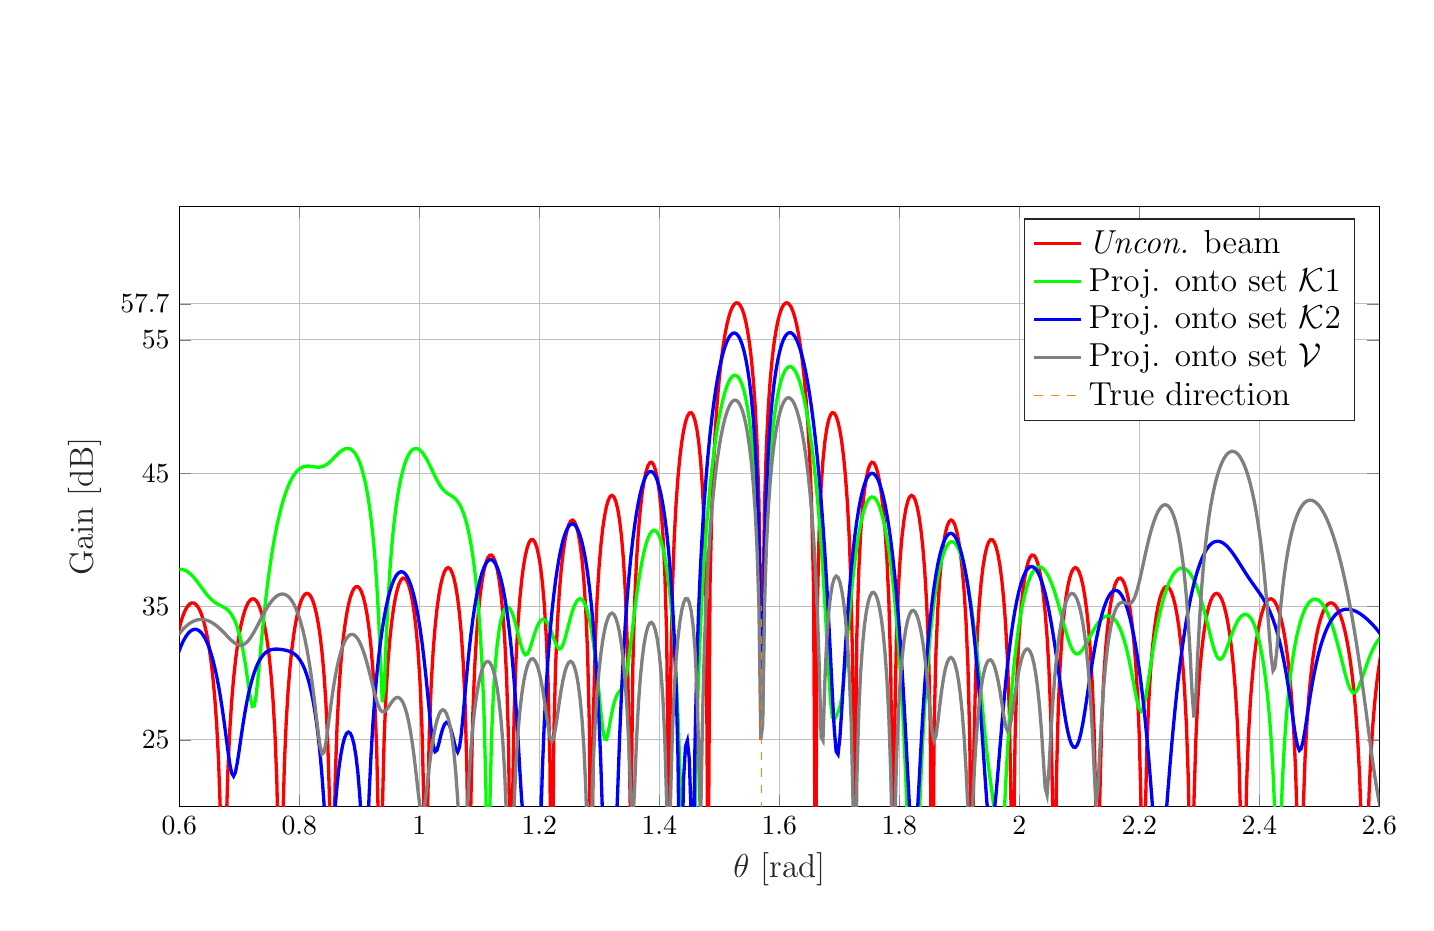
\begin{tikzpicture}

\begin{axis}[%
width=6in,
height=3in,
at={(0.758in,0.481in)},
scale only axis,
xmin=0.6,
xmax=2.6,
xlabel style={font=\large \color{white!15!black}},
xlabel={$\theta~[\mathrm{rad}]$},
ymin=20,
ymax=65,
ytick={25, 35, 45, 55, 57.7},
ylabel style={font=\large \color{white!15!black}},
ylabel={Gain~$[\mathrm{dB}]$},
xmajorgrids,
ymajorgrids,
axis background/.style={fill=white},
legend style={font=\large, legend cell align=left, align=left, draw=white!15!black}
]
\addplot [color=red, line width=1.2pt]
  table[row sep=crcr]{%
0.0031384541993904	34.8929512234198\\
0.00627690839878081	34.892846994354\\
0.00941536259817121	34.8926626310546\\
0.0125538167975616	34.8923821608349\\
0.015692270996952	34.8919832209524\\
0.0188307251963424	34.8914370571422\\
0.0219691793957328	34.8907085211087\\
0.0251076335951232	34.8897560664183\\
0.0282460877945136	34.8885317422337\\
0.031384541993904	34.8869811841477\\
0.0345229961932944	34.8850436012943\\
0.0376614503926848	34.8826517587886\\
0.0407999045920752	34.8797319544329\\
0.0439383587914656	34.8762039885127\\
0.047076812990856	34.8719811253595\\
0.0502152671902464	34.8669700452539\\
0.0533537213896369	34.8610707850904\\
0.0564921755890272	34.8541766660637\\
0.0596306297884176	34.8461742065106\\
0.0627690839878081	34.836943017828\\
0.0659075381871985	34.8263556812157\\
0.0690459923865889	34.8142776027844\\
0.0721844465859793	34.8005668443006\\
0.0753229007853697	34.7850739266045\\
0.0784613549847601	34.7676416023891\\
0.0815998091841505	34.7481045946957\\
0.0847382633835409	34.7262892970768\\
0.0878767175829313	34.7020134308821\\
0.0910151717823217	34.6750856545941\\
0.0941536259817121	34.6453051194984\\
0.0972920801811025	34.6124609652101\\
0.100430534380493	34.5763317477453\\
0.103568988579883	34.5366847917463\\
0.106707442779274	34.4932754573026\\
0.109845896978664	34.4458463103583\\
0.112984351178054	34.3941261840066\\
0.116122805377445	34.3378291159557\\
0.119261259576835	34.2766531450324\\
0.122399713776226	34.2102789467203\\
0.125538167975616	34.1383682842636\\
0.128676622175006	34.0605622476472\\
0.131815076374397	33.9764792477462\\
0.134953530573787	33.8857127267044\\
0.138091984773178	33.7878285380875\\
0.141230438972568	33.6823619410247\\
0.144368893171959	33.5688141410928\\
0.147507347371349	33.4466482963926\\
0.150645801570739	33.315284889408\\
0.15378425577013	33.1740963427517\\
0.15692270996952	33.022400728377\\
0.160061164168911	32.8594543834808\\
0.163199618368301	32.6844431994793\\
0.166338072567691	32.496472289739\\
0.169476526767082	32.2945536622953\\
0.172614980966472	32.0775914188372\\
0.175753435165863	31.844363861235\\
0.178891889365253	31.5935016979631\\
0.182030343564643	31.3234612850484\\
0.185168797764034	31.032491479762\\
0.188307251963424	30.7185921859304\\
0.191445706162815	30.3794619591991\\
0.194584160362205	30.0124310129442\\
0.197722614561595	29.6143744519519\\
0.200861068760986	29.1815982869752\\
0.203999522960376	28.7096872894338\\
0.207137977159767	28.1932982433929\\
0.210276431359157	27.6258732406337\\
0.213414885558547	26.999232767757\\
0.216553339757938	26.302982510563\\
0.219691793957328	25.5236211162388\\
0.222830248156719	24.643147500707\\
0.225968702356109	23.6367877902926\\
0.229107156555499	22.469076171157\\
0.23224561075489	21.0866132193838\\
0.23538406495428	19.4034188281667\\
0.238522519153671	17.2674005130353\\
0.241660973353061	14.3682275901092\\
0.244799427552451	9.89399832243571\\
0.247937881751842	-0.0348459594645641\\
0.251076335951232	1.57398720245486\\
0.254214790150623	10.5841540930961\\
0.257353244350013	14.9541574847176\\
0.260491698549403	17.8686756859255\\
0.263630152748794	20.0592129880311\\
0.266768606948184	21.8138322189111\\
0.269907061147575	23.2758461448407\\
0.273045515346965	24.5269580442147\\
0.276183969546355	25.6181437251214\\
0.279322423745746	26.5833206867292\\
0.282460877945136	27.446169894132\\
0.285599332144527	28.2238535405759\\
0.288737786343917	28.9291828771802\\
0.291876240543307	29.5719519536926\\
0.295014694742698	30.1597948030046\\
0.298153148942088	30.6987566432284\\
0.301291603141479	31.1936862637687\\
0.304430057340869	31.6485126245469\\
0.307568511540259	32.0664441805928\\
0.31070696573965	32.4501152495038\\
0.31384541993904	32.8016952197411\\
0.316983874138431	33.1229711208125\\
0.320122328337821	33.4154107150839\\
0.323260782537211	33.6802110749441\\
0.326399236736602	33.9183361408497\\
0.329537690935992	34.1305457523885\\
0.332676145135383	34.3174179437398\\
0.335814599334773	34.4793657946501\\
0.338953053534163	34.6166497615689\\
0.342091507733554	34.7293861370594\\
0.345229961932944	34.8175520686425\\
0.348368416132335	34.8809873892375\\
0.351506870331725	34.9193933539813\\
0.354645324531115	34.9323282287063\\
0.357783778730506	34.9191995214886\\
0.360922232929896	34.8792524770454\\
0.364060687129287	34.811554249196\\
0.367199141328677	34.7149729090414\\
0.370337595528067	34.5881501085822\\
0.373476049727458	34.4294657615905\\
0.376614503926848	34.2369924666236\\
0.379752958126239	34.0084364903711\\
0.382891412325629	33.7410608109354\\
0.38602986652502	33.4315837606324\\
0.38916832072441	33.0760438276551\\
0.3923067749238	32.6696165315153\\
0.395445229123191	32.2063618498528\\
0.398583683322581	31.6788683964155\\
0.401722137521972	31.0777395675833\\
0.404860591721362	30.3908295619111\\
0.407999045920752	29.6020676779218\\
0.411137500120143	28.6895725635333\\
0.414275954319533	27.6224707842243\\
0.417414408518924	26.3551795156403\\
0.420552862718314	24.8162613418211\\
0.423691316917704	22.8841914234003\\
0.426829771117095	20.3257922611977\\
0.429968225316485	16.5964106808631\\
0.433106679515876	9.80203388674862\\
0.436245133715266	-1.7872955375999\\
0.439383587914656	12.9581612312677\\
0.442522042114047	18.2686731158083\\
0.445660496313437	21.5379942452366\\
0.448798950512828	23.8931760435422\\
0.451937404712218	25.7234643476408\\
0.455075858911608	27.2097350038448\\
0.458214313110999	28.4507405444274\\
0.461352767310389	29.5062184523679\\
0.46449122150978	30.4149597323142\\
0.46762967570917	31.2034832521974\\
0.47076812990856	31.8906259902323\\
0.473906584107951	32.4901570972326\\
0.477045038307341	33.0123540639305\\
0.480183492506732	33.4649970264906\\
0.483321946706122	33.8540188508189\\
0.486460400905512	34.1839420110611\\
0.489598855104903	34.458177881712\\
0.492737309304293	34.6792337132155\\
0.495875763503684	34.8488551264152\\
0.499014217703074	34.9681214765388\\
0.502152671902464	35.0375048093376\\
0.505291126101855	35.0568986667889\\
0.508429580301245	35.0256197064174\\
0.511568034500636	34.942382334423\\
0.514706488700026	34.805243824772\\
0.517844942899416	34.6115142201717\\
0.520983397098807	34.3576210776952\\
0.524121851298197	34.0389129119363\\
0.527260305497588	33.6493754498999\\
0.530398759696978	33.1812187349126\\
0.533537213896368	32.6242653291338\\
0.536675668095759	31.9650195309584\\
0.539814122295149	31.1852014910699\\
0.54295257649454	30.259335461236\\
0.54609103069393	29.1505570667793\\
0.54922948489332	27.8027919449283\\
0.552367939092711	26.1247448355064\\
0.555506393292101	23.9526405203079\\
0.558644847491492	20.9453323165605\\
0.561783301690882	16.1767447373858\\
0.564921755890272	4.82595051473846\\
0.568060210089663	10.4058304527293\\
0.571198664289053	18.1910629523417\\
0.574337118488444	22.2318849347663\\
0.577475572687834	24.9500688764585\\
0.580614026887224	26.9787134016155\\
0.583752481086615	28.5777783959647\\
0.586890935286005	29.879258088738\\
0.590029389485396	30.9591740036202\\
0.593167843684786	31.8651047627285\\
0.596306297884177	32.6285960224688\\
0.599444752083567	33.2714275816352\\
0.602583206282957	33.8090520589761\\
0.605721660482348	34.2526025939754\\
0.608860114681738	34.6101202333085\\
0.611998568881128	34.8873279599812\\
0.615137023080519	35.0881254941322\\
0.618275477279909	35.2149013879558\\
0.6214139314793	35.2687166935709\\
0.62455238567869	35.249389568103\\
0.627690839878081	35.1554936983476\\
0.630829294077471	34.984270404937\\
0.633967748276861	34.7314412288873\\
0.637106202476252	34.3908912050064\\
0.640244656675642	33.9541678618635\\
0.643383110875033	33.4096982405385\\
0.646521565074423	32.7415475796615\\
0.649660019273813	31.927388230597\\
0.652798473473204	30.9350183857352\\
0.655936927672594	29.7160098577815\\
0.659075381871985	28.1931079185544\\
0.662213836071375	26.2322098853677\\
0.665352290270765	23.568812432299\\
0.668490744470156	19.5559741689573\\
0.671629198669546	11.6912190532504\\
0.674767652868937	6.94146000409802\\
0.677906107068327	17.9537798866446\\
0.681044561267717	22.6998595000353\\
0.684183015467108	25.7126064387521\\
0.687321469666498	27.8917661555839\\
0.690459923865889	29.5712138125174\\
0.693598378065279	30.911395267996\\
0.696736832264669	32.0014441411603\\
0.69987528646406	32.8956488531194\\
0.70301374066345	33.6291621648944\\
0.706152194862841	34.2256738923921\\
0.709290649062231	34.7015067984619\\
0.712429103261621	35.0679456562468\\
0.715567557461012	35.3326164653677\\
0.718706011660402	35.5003143011413\\
0.721844465859793	35.5734839383415\\
0.724982920059183	35.5524582924093\\
0.728121374258573	35.4355028573096\\
0.731259828457964	35.2186749429722\\
0.734398282657354	34.8954701935353\\
0.737536736856745	34.4561828670007\\
0.740675191056135	33.8868324519314\\
0.743813645255525	33.1673717493259\\
0.746952099454916	32.2686087297232\\
0.750090553654306	31.1466359644798\\
0.753229007853697	29.7319596332616\\
0.756367462053087	27.90592551877\\
0.759505916252478	25.4411960126928\\
0.762644370451868	21.8108782371099\\
0.765782824651258	15.2281952257448\\
0.768921278850649	3.13641302773942\\
0.772059733050039	17.8631239915564\\
0.775198187249429	23.2113834580099\\
0.77833664144882	26.4504530336619\\
0.78147509564821	28.7382019635788\\
0.784613549847601	30.4713406379844\\
0.787752004046991	31.8329030150391\\
0.790890458246381	32.9219351070474\\
0.794028912445772	33.7975500257441\\
0.797167366645162	34.4973013445652\\
0.800305820844553	35.0459428628088\\
0.803444275043943	35.4600058395585\\
0.806582729243334	35.7503384644633\\
0.809721183442724	35.9235524338068\\
0.812859637642114	35.9828235702162\\
0.815998091841505	35.9282615838413\\
0.819136546040895	35.7569399113734\\
0.822275000240286	35.4625929450413\\
0.825413454439676	35.0349074603027\\
0.828551908639066	34.4582224068002\\
0.831690362838457	33.7092480488982\\
0.834828817037847	32.7529890916488\\
0.837967271237237	31.5350514690707\\
0.841105725436628	29.9658322947139\\
0.844244179636018	27.8837252696265\\
0.847382633835409	24.9517896785555\\
0.850521088034799	20.2586268958812\\
0.85365954223419	9.1444485271695\\
0.85679799643358	14.2931193037801\\
0.85993645063297	22.1377132308637\\
0.863074904832361	26.1611892121205\\
0.866213359031751	28.8295901078495\\
0.869351813231142	30.7828005349423\\
0.872490267430532	32.2821948329478\\
0.875628721629922	33.4595857120364\\
0.878767175829313	34.3900350774152\\
0.881905630028703	35.1195931243934\\
0.885044084228094	35.6777287498891\\
0.888182538427484	36.0835287281626\\
0.891320992626874	36.3490020057323\\
0.894459446826265	36.4808798669732\\
0.897597901025655	36.4815370583261\\
0.900736355225046	36.3493129010163\\
0.903874809424436	36.078322786255\\
0.907013263623826	35.6577079528953\\
0.910151717823217	35.0701026876276\\
0.913290172022607	34.2888088656721\\
0.916428626221997	33.2725532075911\\
0.919567080421388	31.9551948526135\\
0.922705534620778	30.2234838925889\\
0.925843988820169	27.8614720375062\\
0.928982443019559	24.3755659500906\\
0.93212089721895	18.1480109398072\\
0.93525935141834	3.01873765051552\\
0.93839780561773	19.6255519745196\\
0.941536259817121	25.2179278257458\\
0.944674714016511	28.5276622110609\\
0.947813168215902	30.8296086954191\\
0.950951622415292	32.5459422445072\\
0.954090076614682	33.8680112762774\\
0.957228530814073	34.8978937345567\\
0.960366985013463	35.6955167542779\\
0.963505439212854	36.2980245065704\\
0.966643893412244	36.7288709987864\\
0.969782347611634	37.0024530133127\\
0.972920801811025	37.1265408296604\\
0.976059256010415	37.1034672663968\\
0.979197710209806	36.9304812349732\\
0.982336164409196	36.5993780473207\\
0.985474618608586	36.0952897819575\\
0.988613072807977	35.3942224212439\\
0.991751527007367	34.4583641703846\\
0.994889981206758	33.2268692785174\\
0.998028435406148	31.596189334398\\
1.00116688960554	29.3720652471347\\
1.00430534380493	26.1244765681409\\
1.00744379800432	20.5423367830299\\
1.01058225220371	3.19229377161532\\
1.0137207064031	19.5124032498942\\
1.01685916060249	25.7368711692008\\
1.01999761480188	29.2602388967241\\
1.02313606900127	31.6648711027801\\
1.02627452320066	33.436077183062\\
1.02941297740005	34.7862005122603\\
1.03255143159944	35.8260826663514\\
1.03568988579883	36.6197142750691\\
1.03882833999822	37.2060947362216\\
1.04196679419761	37.6092824639475\\
1.045105248397	37.843404020014\\
1.04824370259639	37.9151849881574\\
1.05138215679578	37.8250575392633\\
1.05452061099518	37.5672494932493\\
1.05765906519457	37.1288861767315\\
1.06079751939396	36.4877828117593\\
1.06393597359335	35.6080361192082\\
1.06707442779274	34.4312582676992\\
1.07021288199213	32.857881086978\\
1.07335133619152	30.7018678304183\\
1.07648979039091	27.5558747462077\\
1.0796282445903	22.2087825344637\\
1.08276669878969	5.92694912931209\\
1.08590515298908	20.1475863319946\\
1.08904360718847	26.6857473515411\\
1.09218206138786	30.3061234217213\\
1.09532051558725	32.7537450559651\\
1.09845896978664	34.5440769935904\\
1.10159742398603	35.89896286441\\
1.10473587818542	36.9329590158688\\
1.10787433238481	37.7115458859282\\
1.1110127865842	38.2741131368734\\
1.11415124078359	38.6444037402467\\
1.11728969498298	38.8356280911327\\
1.12042814918237	38.852937678211\\
1.12356660338176	38.6943285809307\\
1.12670505758115	38.3503242318137\\
1.12984351178054	37.8023179617131\\
1.13298196597994	37.0189033579101\\
1.13612042017933	35.9484499151874\\
1.13925887437872	34.5034580754401\\
1.14239732857811	32.523794366457\\
1.1455357827775	29.6728924485652\\
1.14867423697689	25.0335338812364\\
1.15181269117628	13.6951507375313\\
1.15495114537567	19.0003347829647\\
1.15808959957506	26.9608886939105\\
1.16122805377445	30.9882191930634\\
1.16436650797384	33.6309290033722\\
1.16750496217323	35.5355187448621\\
1.17064341637262	36.9639211446183\\
1.17378187057201	38.0469293553269\\
1.1769203247714	38.8576903337832\\
1.18005877897079	39.4394909618061\\
1.18319723317018	39.8180187990344\\
1.18633568736957	40.0072283041216\\
1.18947414156896	40.0121021380377\\
1.19261259576835	39.8295751335462\\
1.19575104996774	39.4480007364416\\
1.19888950416713	38.8449440353582\\
1.20202795836652	37.9823267372174\\
1.20516641256591	36.7963616753682\\
1.20830486676531	35.1753720199125\\
1.2114433209647	32.9038828282505\\
1.21458177516409	29.4854144608262\\
1.21772022936348	23.2694518354499\\
1.22085868356287	5.83549290361533\\
1.22399713776226	24.8477662578215\\
1.22713559196165	30.4782743565734\\
1.23027404616104	33.7879824520801\\
1.23341250036043	36.06970455298\\
1.23655095455982	37.7471455831803\\
1.23968940875921	39.0109869278378\\
1.2428278629586	39.9617730417789\\
1.24596631715799	40.6571683633166\\
1.24910477135738	41.1311950128701\\
1.25224322555677	41.4030417275967\\
1.25538167975616	41.4812289203132\\
1.25852013395555	41.3652811409643\\
1.26165858815494	41.0456514783001\\
1.26479704235433	40.5018661415863\\
1.26793549655372	39.6980559693983\\
1.27107395075311	38.573524940995\\
1.2742124049525	37.0219964835552\\
1.27735085915189	34.8398708833831\\
1.28048931335128	31.5656606539295\\
1.28362776755067	25.7243018411309\\
1.28676622175007	3.28876539954894\\
1.28990467594946	26.0109333039082\\
1.29304313014885	31.9814573114136\\
1.29618158434824	35.4189860058402\\
1.29932003854763	37.7723098973527\\
1.30245849274702	39.4973288848972\\
1.30559694694641	40.7954968479535\\
1.3087354011458	41.7718728100005\\
1.31187385534519	42.4862071852826\\
1.31501230954458	42.9734407796414\\
1.31815076374397	43.2529824332241\\
1.32128921794336	43.3330276464366\\
1.32442767214275	43.2122087887118\\
1.32756612634214	42.8793340081648\\
1.33070458054153	42.3110998743061\\
1.33384303474092	41.4666956303538\\
1.33698148894031	40.2762624788923\\
1.3401199431397	38.6147196489325\\
1.34325839733909	36.2331771887701\\
1.34639685153848	32.5269056446761\\
1.34953530573787	25.2031355867997\\
1.35267375993726	17.1920328089721\\
1.35581221413665	30.3429821463429\\
1.35895066833604	35.3619549301961\\
1.36208912253543	38.458410000597\\
1.36522757673483	40.6379905335335\\
1.36836603093422	42.25791538033\\
1.37150448513361	43.4849702648383\\
1.374642939333	44.4086678238327\\
1.37778139353239	45.0804826792778\\
1.38091984773178	45.5302243314088\\
1.38405830193117	45.7735516719531\\
1.38719675613056	45.8153549795733\\
1.39033521032995	45.6507265567632\\
1.39347366452934	45.2639623590877\\
1.39661211872873	44.6251388318729\\
1.39975057292812	43.6825181711204\\
1.40288902712751	42.3459865370028\\
1.4060274813269	40.4472816420406\\
1.40916593552629	37.6248450457488\\
1.41230438972568	32.8540855266063\\
1.41544284392507	19.5824961638675\\
1.41858129812446	28.54145103323\\
1.42171975232385	36.0800167181305\\
1.42485820652324	40.0599648964796\\
1.42799666072263	42.729099979661\\
1.43113511492202	44.6846960913204\\
1.43427356912141	46.1734427053108\\
1.4374120233208	47.3196148523086\\
1.44055047752019	48.1927654454487\\
1.44368893171959	48.8336102665068\\
1.44682738591898	49.2654497578748\\
1.44996584011837	49.4995003307501\\
1.45310429431776	49.537129979947\\
1.45624274851715	49.3700555962041\\
1.45938120271654	48.9785871525106\\
1.46251965691593	48.3271023444389\\
1.46565811111532	47.3543110581976\\
1.46879656531471	45.9515955331617\\
1.4719350195141	43.9083812402377\\
1.47507347371349	40.7395690505915\\
1.47821192791288	34.8403653440559\\
1.48135038211227	11.6045611224286\\
1.48448883631166	36.4416175572715\\
1.48762729051105	42.4407696121813\\
1.49076574471044	46.0497388889833\\
1.49390419890983	48.625534144798\\
1.49704265310922	50.6065461877332\\
1.50018110730861	52.1905145236025\\
1.503319561508	53.4833983238501\\
1.50645801570739	54.5482824822571\\
1.50959646990678	55.4253899958286\\
1.51273492410617	56.141515608661\\
1.51587337830556	56.7149289254334\\
1.51901183250496	57.1581001968617\\
1.52215028670435	57.4792771162726\\
1.52528874090374	57.683400159692\\
1.52842719510313	57.772598041486\\
1.53156564930252	57.7463797971894\\
1.53470410350191	57.6015655192873\\
1.5378425577013	57.3319400381606\\
1.54098101190069	56.9275499059855\\
1.54411946610008	56.3734670080263\\
1.54725792029947	55.6476625106701\\
1.55039637449886	54.7172580036849\\
1.55353482869825	53.5315417450898\\
1.55667328289764	52.0078321598104\\
1.55981173709703	49.99923475191\\
1.56295019129642	47.2067381393144\\
1.56608864549581	42.8561648618556\\
1.5692270996952	33.3568491370331\\
1.57236555389459	33.3568491370331\\
1.57550400809398	42.8561648618556\\
1.57864246229337	47.2067381393144\\
1.58178091649276	49.99923475191\\
1.58491937069215	52.0078321598104\\
1.58805782489154	53.5315417450899\\
1.59119627909093	54.7172580036849\\
1.59433473329032	55.6476625106701\\
1.59747318748972	56.3734670080263\\
1.60061164168911	56.9275499059856\\
1.6037500958885	57.3319400381606\\
1.60688855008789	57.6015655192873\\
1.61002700428728	57.7463797971894\\
1.61316545848667	57.772598041486\\
1.61630391268606	57.683400159692\\
1.61944236688545	57.4792771162726\\
1.62258082108484	57.1581001968617\\
1.62571927528423	56.7149289254334\\
1.62885772948362	56.141515608661\\
1.63199618368301	55.4253899958287\\
1.6351346378824	54.5482824822571\\
1.63827309208179	53.4833983238502\\
1.64141154628118	52.1905145236025\\
1.64455000048057	50.6065461877332\\
1.64768845467996	48.625534144798\\
1.65082690887935	46.0497388889831\\
1.65396536307874	42.4407696121816\\
1.65710381727813	36.4416175572711\\
1.66024227147752	11.6045611224214\\
1.66338072567691	34.8403653440565\\
1.6665191798763	40.7395690505912\\
1.66965763407569	43.908381240238\\
1.67279608827508	45.9515955331617\\
1.67593454247447	47.3543110581976\\
1.67907299667387	48.327102344439\\
1.68221145087326	48.9785871525106\\
1.68534990507265	49.3700555962042\\
1.68848835927204	49.537129979947\\
1.69162681347143	49.4995003307501\\
1.69476526767082	49.2654497578748\\
1.69790372187021	48.8336102665068\\
1.7010421760696	48.1927654454487\\
1.70418063026899	47.3196148523085\\
1.70731908446838	46.1734427053108\\
1.71045753866777	44.6846960913205\\
1.71359599286716	42.7290999796608\\
1.71673444706655	40.0599648964799\\
1.71987290126594	36.0800167181294\\
1.72301135546533	28.5414510332294\\
1.72614980966472	19.5824961638666\\
1.72928826386411	32.8540855266063\\
1.7324267180635	37.6248450457488\\
1.73556517226289	40.4472816420406\\
1.73870362646228	42.3459865370028\\
1.74184208066167	43.6825181711204\\
1.74498053486106	44.6251388318727\\
1.74811898906045	45.2639623590875\\
1.75125744325984	45.6507265567632\\
1.75439589745924	45.8153549795733\\
1.75753435165863	45.7735516719531\\
1.76067280585802	45.5302243314088\\
1.76381126005741	45.0804826792779\\
1.7669497142568	44.4086678238327\\
1.77008816845619	43.4849702648384\\
1.77322662265558	42.2579153803304\\
1.77636507685497	40.6379905335332\\
1.77950353105436	38.458410000597\\
1.78264198525375	35.3619549301961\\
1.78578043945314	30.3429821463431\\
1.78891889365253	17.192032808972\\
1.79205734785192	25.2031355868004\\
1.79519580205131	32.5269056446756\\
1.7983342562507	36.2331771887701\\
1.80147271045009	38.6147196489323\\
1.80461116464948	40.2762624788925\\
1.80774961884887	41.4666956303538\\
1.81088807304826	42.311099874306\\
1.81402652724765	42.8793340081648\\
1.81716498144704	43.2122087887118\\
1.82030343564643	43.3330276464366\\
1.82344188984582	43.2529824332242\\
1.82658034404521	42.9734407796415\\
1.8297187982446	42.4862071852828\\
1.83285725244399	41.7718728100007\\
1.83599570664339	40.795496847953\\
1.83913416084278	39.4973288848971\\
1.84227261504217	37.7723098973533\\
1.84541106924156	35.4189860058403\\
1.84854952344095	31.981457311414\\
1.85168797764034	26.0109333039079\\
1.85482643183973	3.28876539954982\\
1.85796488603912	25.7243018411308\\
1.86110334023851	31.5656606539295\\
1.8642417944379	34.8398708833832\\
1.86738024863729	37.0219964835551\\
1.87051870283668	38.573524940995\\
1.87365715703607	39.6980559693984\\
1.87679561123546	40.5018661415866\\
1.87993406543485	41.0456514783005\\
1.88307251963424	41.3652811409642\\
1.88621097383363	41.481228920313\\
1.88934942803302	41.4030417275968\\
1.89248788223241	41.1311950128701\\
1.8956263364318	40.6571683633168\\
1.89876479063119	39.9617730417787\\
1.90190324483058	39.0109869278379\\
1.90504169902997	37.7471455831803\\
1.90818015322936	36.0697045529793\\
1.91131860742876	33.7879824520803\\
1.91445706162815	30.4782743565724\\
1.91759551582754	24.8477662578211\\
1.92073397002693	5.83549290360382\\
1.92387242422632	23.2694518354487\\
1.92701087842571	29.4854144608266\\
1.9301493326251	32.9038828282506\\
1.93328778682449	35.1753720199127\\
1.93642624102388	36.7963616753682\\
1.93956469522327	37.982326737217\\
1.94270314942266	38.8449440353586\\
1.94584160362205	39.4480007364411\\
1.94898005782144	39.8295751335465\\
1.95211851202083	40.0121021380376\\
1.95525696622022	40.0072283041218\\
1.95839542041961	39.8180187990343\\
1.961533874619	39.4394909618062\\
1.96467232881839	38.8576903337826\\
1.96781078301778	38.0469293553271\\
1.97094923721717	36.9639211446183\\
1.97408769141656	35.5355187448615\\
1.97722614561595	33.6309290033731\\
1.98036459981534	30.988219193064\\
1.98350305401473	26.9608886939105\\
1.98664150821412	19.0003347829646\\
1.98977996241352	13.6951507375245\\
1.99291841661291	25.0335338812366\\
1.9960568708123	29.6728924485652\\
1.99919532501169	32.5237943664571\\
2.00233377921108	34.5034580754404\\
2.00547223341047	35.9484499151873\\
2.00861068760986	37.0189033579101\\
2.01174914180925	37.8023179617134\\
2.01488759600864	38.3503242318139\\
2.01802605020803	38.6943285809307\\
2.02116450440742	38.8529376782113\\
2.02430295860681	38.8356280911329\\
2.0274414128062	38.644403740246\\
2.03057986700559	38.274113136873\\
2.03371832120498	37.7115458859282\\
2.03685677540437	36.9329590158688\\
2.03999522960376	35.8989628644091\\
2.04313368380315	34.5440769935902\\
2.04627213800254	32.7537450559653\\
2.04941059220193	30.3061234217194\\
2.05254904640132	26.6857473515406\\
2.05568750060071	20.1475863320004\\
2.0588259548001	5.92694912930968\\
2.06196440899949	22.2087825344688\\
2.06510286319888	27.5558747462077\\
2.06824131739828	30.7018678304182\\
2.07137977159767	32.8578810869779\\
2.07451822579706	34.4312582676995\\
2.07765667999645	35.608036119208\\
2.08079513419584	36.4877828117586\\
2.08393358839523	37.1288861767316\\
2.08707204259462	37.5672494932489\\
2.09021049679401	37.8250575392636\\
2.0933489509934	37.9151849881575\\
2.09648740519279	37.843404020014\\
2.09962585939218	37.6092824639474\\
2.10276431359157	37.2060947362214\\
2.10590276779096	36.619714275069\\
2.10904122199035	35.8260826663515\\
2.11217967618974	34.786200512261\\
2.11531813038913	33.4360771830622\\
2.11845658458852	31.6648711027794\\
2.12159503878791	29.2602388967243\\
2.1247334929873	25.7368711692009\\
2.12787194718669	19.512403249895\\
2.13101040138608	3.19229377160858\\
2.13414885558547	20.5423367830313\\
2.13728730978486	26.1244765681411\\
2.14042576398425	29.3720652471347\\
2.14356421818364	31.5961893343979\\
2.14670267238304	33.2268692785174\\
2.14984112658243	34.4583641703846\\
2.15297958078182	35.3942224212423\\
2.15611803498121	36.0952897819575\\
2.1592564891806	36.5993780473207\\
2.16239494337999	36.9304812349732\\
2.16553339757938	37.1034672663973\\
2.16867185177877	37.1265408296605\\
2.17181030597816	37.0024530133127\\
2.17494876017755	36.7288709987864\\
2.17808721437694	36.2980245065702\\
2.18122566857633	35.6955167542773\\
2.18436412277572	34.8978937345565\\
2.18750257697511	33.8680112762778\\
2.1906410311745	32.5459422445067\\
2.19377948537389	30.8296086954192\\
2.19691793957328	28.5276622110616\\
2.20005639377267	25.2179278257458\\
2.20319484797206	19.6255519745141\\
2.20633330217145	3.01873765051481\\
2.20947175637084	18.1480109398061\\
2.21261021057023	24.3755659500915\\
2.21574866476962	27.8614720375066\\
2.21888711896901	30.2234838925893\\
2.22202557316841	31.9551948526136\\
2.2251640273678	33.2725532075908\\
2.22830248156719	34.2888088656723\\
2.23144093576658	35.0701026876282\\
2.23457938996597	35.6577079528954\\
2.23771784416536	36.0783227862551\\
2.24085629836475	36.3493129010164\\
2.24399475256414	36.4815370583257\\
2.24713320676353	36.4808798669733\\
2.25027166096292	36.3490020057322\\
2.25341011516231	36.0835287281628\\
2.2565485693617	35.6777287498891\\
2.25968702356109	35.1195931243934\\
2.26282547776048	34.3900350774154\\
2.26596393195987	33.4595857120363\\
2.26910238615926	32.2821948329478\\
2.27224084035865	30.7828005349426\\
2.27537929455804	28.8295901078494\\
2.27851774875743	26.1611892121196\\
2.28165620295682	22.1377132308628\\
2.28479465715621	14.2931193037812\\
2.2879331113556	9.14444852716938\\
2.29107156555499	20.2586268958808\\
2.29421001975438	24.951789678556\\
2.29734847395377	27.8837252696261\\
2.30048692815316	29.9658322947138\\
2.30362538235256	31.5350514690716\\
2.30676383655195	32.7529890916487\\
2.30990229075134	33.709248048898\\
2.31304074495073	34.4582224068001\\
2.31617919915012	35.034907460303\\
2.31931765334951	35.4625929450412\\
2.3224561075489	35.7569399113739\\
2.32559456174829	35.9282615838416\\
2.32873301594768	35.9828235702163\\
2.33187147014707	35.9235524338071\\
2.33500992434646	35.7503384644644\\
2.33814837854585	35.4600058395584\\
2.34128683274524	35.0459428628091\\
2.34442528694463	34.4973013445653\\
2.34756374114402	33.7975500257441\\
2.35070219534341	32.9219351070477\\
2.3538406495428	31.832903015039\\
2.35697910374219	30.4713406379857\\
2.36011755794158	28.7382019635788\\
2.36325601214097	26.4504530336616\\
2.36639446634036	23.2113834580091\\
2.36953292053975	17.863123991558\\
2.37267137473914	3.13641302773091\\
2.37580982893853	15.2281952257434\\
2.37894828313792	21.8108782371068\\
2.38208673733732	25.4411960126935\\
2.38522519153671	27.9059255187693\\
2.3883636457361	29.7319596332622\\
2.39150209993549	31.1466359644799\\
2.39464055413488	32.2686087297232\\
2.39777900833427	33.1673717493263\\
2.40091746253366	33.8868324519312\\
2.40405591673305	34.4561828670008\\
2.40719437093244	34.8954701935352\\
2.41033282513183	35.218674942973\\
2.41347127933122	35.4355028573096\\
2.41660973353061	35.5524582924091\\
2.41974818773	35.5734839383413\\
2.42288664192939	35.5003143011412\\
2.42602509612878	35.3326164653678\\
2.42916355032817	35.0679456562459\\
2.43230200452756	34.7015067984616\\
2.43544045872695	34.2256738923919\\
2.43857891292634	33.6291621648949\\
2.44171736712573	32.8956488531188\\
2.44485582132512	32.0014441411603\\
2.44799427552451	30.9113952679966\\
2.4511327297239	29.5712138125179\\
2.4542711839233	27.8917661555843\\
2.45740963812269	25.7126064387513\\
2.46054809232208	22.6998595000364\\
2.46368654652147	17.9537798866459\\
2.46682500072086	6.94146000408388\\
2.46996345492025	11.6912190532487\\
2.47310190911964	19.5559741689568\\
2.47624036331903	23.5688124322981\\
2.47937881751842	26.2322098853671\\
2.48251727171781	28.1931079185536\\
2.4856557259172	29.7160098577806\\
2.48879418011659	30.935018385736\\
2.49193263431598	31.9273882305972\\
2.49507108851537	32.7415475796615\\
2.49820954271476	33.4096982405381\\
2.50134799691415	33.9541678618635\\
2.50448645111354	34.3908912050063\\
2.50762490531293	34.7314412288873\\
2.51076335951232	34.9842704049371\\
2.51390181371171	35.1554936983473\\
2.5170402679111	35.249389568103\\
2.52017872211049	35.2687166935709\\
2.52331717630988	35.2149013879555\\
2.52645563050927	35.0881254941323\\
2.52959408470866	34.887327959981\\
2.53273253890806	34.6101202333094\\
2.53587099310745	34.2526025939752\\
2.53900944730684	33.8090520589768\\
2.54214790150623	33.2714275816349\\
2.54528635570562	32.6285960224686\\
2.54842480990501	31.865104762729\\
2.5515632641044	30.9591740036199\\
2.55470171830379	29.8792580887385\\
2.55784017250318	28.5777783959654\\
2.56097862670257	26.9787134016157\\
2.56411708090196	24.9500688764591\\
2.56725553510135	22.2318849347638\\
2.57039398930074	18.1910629523434\\
2.57353244350013	10.405830452719\\
2.57667089769952	4.8259505147512\\
2.57980935189891	16.1767447373884\\
2.5829478060983	20.9453323165605\\
2.58608626029769	23.9526405203073\\
2.58922471449708	26.1247448355072\\
2.59236316869647	27.802791944929\\
2.59550162289586	29.150557066779\\
2.59864007709525	30.2593354612359\\
2.60177853129464	31.1852014910699\\
2.60491698549403	31.9650195309583\\
2.60805543969342	32.6242653291338\\
2.61119389389282	33.1812187349124\\
2.61433234809221	33.6493754498999\\
2.6174708022916	34.0389129119363\\
2.62060925649099	34.357621077695\\
2.62374771069038	34.6115142201721\\
2.62688616488977	34.8052438247721\\
2.63002461908916	34.9423823344224\\
2.63316307328855	35.0256197064174\\
2.63630152748794	35.0568986667888\\
2.63943998168733	35.0375048093374\\
2.64257843588672	34.9681214765388\\
2.64571689008611	34.8488551264149\\
2.6488553442855	34.6792337132153\\
2.65199379848489	34.4581778817119\\
2.65513225268428	34.1839420110608\\
2.65827070688367	33.8540188508185\\
2.66140916108306	33.4649970264904\\
2.66454761528245	33.0123540639297\\
2.66768606948184	32.4901570972318\\
2.67082452368123	31.8906259902317\\
2.67396297788062	31.2034832521969\\
2.67710143208001	30.4149597323138\\
2.6802398862794	29.5062184523681\\
2.68337834047879	28.4507405444268\\
2.68651679467818	27.2097350038463\\
2.68965524887758	25.7234643476407\\
2.69279370307697	23.8931760435415\\
2.69593215727636	21.5379942452369\\
2.69907061147575	18.2686731158081\\
2.70220906567514	12.9581612312625\\
2.70534751987453	-1.78729553761765\\
2.70848597407392	9.80203388675319\\
2.71162442827331	16.5964106808632\\
2.7147628824727	20.3257922611947\\
2.71790133667209	22.8841914234005\\
2.72103979087148	24.8162613418221\\
2.72417824507087	26.3551795156404\\
2.72731669927026	27.6224707842252\\
2.73045515346965	28.6895725635342\\
2.73359360766904	29.6020676779234\\
2.73673206186843	30.3908295619111\\
2.73987051606782	31.0777395675836\\
2.74300897026721	31.6788683964157\\
2.7461474244666	32.2063618498529\\
2.74928587866599	32.6696165315152\\
2.75242433286538	33.0760438276549\\
2.75556278706477	33.4315837606326\\
2.75870124126416	33.7410608109352\\
2.76183969546355	34.0084364903713\\
2.76497814966294	34.2369924666234\\
2.76811660386234	34.4294657615908\\
2.77125505806173	34.5881501085821\\
2.77439351226112	34.7149729090414\\
2.77753196646051	34.8115542491957\\
2.7806704206599	34.8792524770453\\
2.78380887485929	34.9191995214887\\
2.78694732905868	34.9323282287071\\
2.79008578325807	34.9193933539816\\
2.79322423745746	34.8809873892382\\
2.79636269165685	34.8175520686424\\
2.79950114585624	34.7293861370594\\
2.80263960005563	34.6166497615689\\
2.80577805425502	34.4793657946502\\
2.80891650845441	34.3174179437402\\
2.8120549626538	34.1305457523884\\
2.81519341685319	33.9183361408497\\
2.81833187105258	33.680211074944\\
2.82147032525197	33.4154107150839\\
2.82460877945136	33.1229711208118\\
2.82774723365075	32.801695219741\\
2.83088568785014	32.4501152495045\\
2.83402414204953	32.066444180593\\
2.83716259624892	31.6485126245472\\
2.84030105044831	31.1936862637688\\
2.84343950464771	30.6987566432286\\
2.8465779588471	30.159794803004\\
2.84971641304649	29.5719519536918\\
2.85285486724588	28.9291828771796\\
2.85599332144527	28.2238535405763\\
2.85913177564466	27.4461698941315\\
2.86227022984405	26.5833206867295\\
2.86540868404344	25.6181437251215\\
2.86854713824283	24.5269580442135\\
2.87168559244222	23.2758461448407\\
2.87482404664161	21.8138322189098\\
2.877962500841	20.059212988028\\
2.88110095504039	17.8686756859229\\
2.88423940923978	14.9541574847168\\
2.88737786343917	10.5841540930913\\
2.89051631763856	1.57398720244404\\
2.89365477183795	-0.0348459594175594\\
2.89679322603734	9.89399832244036\\
2.89993168023673	14.368227590109\\
2.90307013443612	17.2674005130374\\
2.90620858863551	19.4034188281644\\
2.9093470428349	21.0866132193863\\
2.91248549703429	22.4690761711568\\
2.91562395123368	23.6367877902925\\
2.91876240543307	24.6431475007074\\
2.92190085963247	25.5236211162391\\
2.92503931383186	26.3029825105638\\
2.92817776803125	26.9992327677569\\
2.93131622223064	27.6258732406325\\
2.93445467643003	28.1932982433942\\
2.93759313062942	28.7096872894356\\
2.94073158482881	29.1815982869748\\
2.9438700390282	29.6143744519524\\
2.94700849322759	30.0124310129451\\
2.95014694742698	30.3794619591993\\
2.95328540162637	30.7185921859312\\
2.95642385582576	31.0324914797624\\
2.95956231002515	31.3234612850485\\
2.96270076422454	31.5935016979634\\
2.96583921842393	31.8443638612349\\
2.96897767262332	32.0775914188379\\
2.97211612682271	32.2945536622954\\
2.9752545810221	32.4964722897395\\
2.97839303522149	32.6844431994795\\
2.98153148942088	32.8594543834813\\
2.98466994362027	33.0224007283771\\
2.98780839781966	33.1740963427521\\
2.99094685201905	33.3152848894083\\
2.99408530621844	33.4466482963925\\
2.99722376041783	33.5688141410928\\
3.00036221461722	33.6823619410249\\
3.00350066881662	33.7878285380873\\
3.00663912301601	33.8857127267045\\
3.0097775772154	33.9764792477462\\
3.01291603141479	34.0605622476479\\
3.01605448561418	34.1383682842639\\
3.01919293981357	34.2102789467205\\
3.02233139401296	34.2766531450326\\
3.02546984821235	34.3378291159561\\
3.02860830241174	34.3941261840078\\
3.03174675661113	34.4458463103584\\
3.03488521081052	34.4932754573028\\
3.03802366500991	34.5366847917469\\
3.0411621192093	34.5763317477455\\
3.04430057340869	34.61246096521\\
3.04743902760808	34.6453051194987\\
3.05057748180747	34.6750856545942\\
3.05371593600686	34.7020134308825\\
3.05685439020625	34.7262892970767\\
3.05999284440564	34.748104594696\\
3.06313129860503	34.7676416023895\\
3.06626975280442	34.7850739266047\\
3.06940820700381	34.8005668443006\\
3.0725466612032	34.8142776027849\\
3.07568511540259	34.8263556812161\\
3.07882356960198	34.8369430178283\\
3.08196202380138	34.8461742065107\\
3.08510047800077	34.8541766660639\\
3.08823893220016	34.8610707850905\\
3.09137738639955	34.8669700452542\\
3.09451584059894	34.8719811253596\\
3.09765429479833	34.876203988513\\
3.10079274899772	34.8797319544332\\
3.10393120319711	34.8826517587887\\
3.1070696573965	34.8850436012945\\
3.11020811159589	34.886981184148\\
3.11334656579528	34.888531742234\\
3.11648501999467	34.8897560664185\\
3.11962347419406	34.8907085211088\\
3.12276192839345	34.8914370571425\\
3.12590038259284	34.8919832209525\\
3.12903883679223	34.8923821608355\\
3.13217729099162	34.8926626310547\\
3.13531574519101	34.892846994354\\
3.1384541993904	34.8929512234199\\
};
\addlegendentry{\emph{Uncon.} beam}


\addplot [color=green, line width=1.2pt]
  table[row sep=crcr]{%
0.0031384541993904	27.4371946765552\\
0.00627690839878081	27.4340026620587\\
0.00941536259817121	27.4286787292323\\
0.0125538167975616	27.4212170302074\\
0.015692270996952	27.411609408828\\
0.0188307251963424	27.399845432854\\
0.0219691793957328	27.3859124374002\\
0.0251076335951232	27.3697955810298\\
0.0282460877945136	27.3514779165135\\
0.031384541993904	27.3309404785598\\
0.0345229961932944	27.3081623913386\\
0.0376614503926848	27.283120999074\\
0.0407999045920752	27.2557920236418\\
0.0439383587914656	27.2261497536512\\
0.047076812990856	27.1941672702177\\
0.0502152671902464	27.159816715438\\
0.0533537213896369	27.1230696104735\\
0.0564921755890272	27.0838972310884\\
0.0596306297884176	27.0422710496841\\
0.0627690839878081	26.9981632540291\\
0.0659075381871985	26.9515473543604\\
0.0690459923865889	26.902398892025\\
0.0721844465859793	26.8506962645421\\
0.0753229007853697	26.7964216838584\\
0.0784613549847601	26.7395622865345\\
0.0815998091841505	26.6801114167577\\
0.0847382633835409	26.6180701053558\\
0.0878767175829313	26.5534487701235\\
0.0910151717823217	26.4862691650617\\
0.0941536259817121	26.4165666080135\\
0.0972920801811025	26.3443925176441\\
0.100430534380493	26.2698172916808\\
0.103568988579883	26.1929335577034\\
0.106707442779274	26.1138598260641\\
0.109845896978664	26.0327445699981\\
0.112984351178054	25.9497707505671\\
0.116122805377445	25.8651607922065\\
0.119261259576835	25.779181997204\\
0.122399713776226	25.6921523629495\\
0.125538167975616	25.6044467323235\\
0.128676622175006	25.5165031636756\\
0.131815076374397	25.4288293506996\\
0.134953530573787	25.3420088531005\\
0.138091984773178	25.25670681617\\
0.141230438972568	25.1736747627343\\
0.144368893171959	25.0937539387529\\
0.147507347371349	25.0178765914668\\
0.150645801570739	24.9470644691314\\
0.15378425577013	24.8824237709175\\
0.15692270996952	24.8251357673837\\
0.160061164168911	24.7764423819526\\
0.163199618368301	24.7376261981075\\
0.166338072567691	24.70998465717\\
0.169476526767082	24.6947986443601\\
0.172614980966472	24.6932962133223\\
0.175753435165863	24.7066128278049\\
0.178891889365253	24.7357501292168\\
0.182030343564643	24.78153576978\\
0.185168797764034	24.8445871711587\\
0.188307251963424	24.9252820812161\\
0.191445706162815	25.0237384505075\\
0.194584160362205	25.1398054451967\\
0.197722614561595	25.2730664350178\\
0.200861068760986	25.4228536870207\\
0.203999522960376	25.588273429513\\
0.207137977159767	25.7682390899789\\
0.210276431359157	25.961509970305\\
0.213414885558547	26.1667324503007\\
0.216553339757938	26.3824809814731\\
0.219691793957328	26.6072965684289\\
0.222830248156719	26.8397210279212\\
0.225968702356109	27.0783259559839\\
0.229107156555499	27.3217359330829\\
0.23224561075489	27.5686459955794\\
0.23538406495428	27.8178337710826\\
0.238522519153671	28.0681669128829\\
0.241660973353061	28.3186065898261\\
0.244799427552451	28.5682078171005\\
0.247937881751842	28.8161173771634\\
0.251076335951232	29.061570003042\\
0.254214790150623	29.3038833987855\\
0.257353244350013	29.5424525684251\\
0.260491698549403	29.77674382581\\
0.263630152748794	30.0062887685537\\
0.266768606948184	30.2306784231437\\
0.269907061147575	30.4495577054272\\
0.273045515346965	30.6626202908215\\
0.276183969546355	30.8696039499207\\
0.279322423745746	31.0702863763037\\
0.282460877945136	31.2644815124096\\
0.285599332144527	31.4520363644915\\
0.288737786343917	31.6328282878055\\
0.291876240543307	31.8067627167703\\
0.295014694742698	31.97377131096\\
0.298153148942088	32.1338104856411\\
0.301291603141479	32.2868602944305\\
0.304430057340869	32.4329236309858\\
0.307568511540259	32.5720257161689\\
0.31070696573965	32.7042138362361\\
0.31384541993904	32.8295572964341\\
0.316983874138431	32.9481475523345\\
0.320122328337821	33.0600984784894\\
0.323260782537211	33.1655467302006\\
0.326399236736602	33.2646521495713\\
0.329537690935992	33.3575981612978\\
0.332676145135383	33.4445920972948\\
0.335814599334773	33.5258653821211\\
0.338953053534163	33.6016735039459\\
0.342091507733554	33.6722956886089\\
0.345229961932944	33.7380341881984\\
0.348368416132335	33.7992130909597\\
0.351506870331725	33.8561765575655\\
0.354645324531115	33.9092863906693\\
0.357783778730506	33.9589188516872\\
0.360922232929896	34.0054606519108\\
0.364060687129287	34.0493040654384\\
0.367199141328677	34.0908411397884\\
0.370337595528067	34.130457016379\\
0.373476049727458	34.1685224169686\\
0.376614503926848	34.2053854017909\\
0.379752958126239	34.2413625582125\\
0.382891412325629	34.2767298313282\\
0.38602986652502	34.3117132557409\\
0.38916832072441	34.3464798857458\\
0.3923067749238	34.3811292443583\\
0.395445229123191	34.4156856158787\\
0.398583683322581	34.4500914892401\\
0.401722137521972	34.4842024194243\\
0.404860591721362	34.5177835134875\\
0.407999045920752	34.5505076702336\\
0.411137500120143	34.5819556146125\\
0.414275954319533	34.6116176771102\\
0.417414408518924	34.6388971829009\\
0.420552862718314	34.6631152431348\\
0.423691316917704	34.6835166876315\\
0.426829771117095	34.6992768489187\\
0.429968225316485	34.7095089041152\\
0.433106679515876	34.7132715037304\\
0.436245133715266	34.7095764637595\\
0.439383587914656	34.6973963674393\\
0.442522042114047	34.6756720139179\\
0.445660496313437	34.6433197625407\\
0.448798950512828	34.5992389552169\\
0.451937404712218	34.5423197606182\\
0.455075858911608	34.4714519823622\\
0.458214313110999	34.3855356239877\\
0.461352767310389	34.2834943284987\\
0.46449122150978	34.1642932400042\\
0.46762967570917	34.0269634096568\\
0.47076812990856	33.8706356377236\\
0.473906584107951	33.6945876649472\\
0.477045038307341	33.4983099524885\\
0.480183492506732	33.2815969422129\\
0.483321946706122	33.0446725973444\\
0.486460400905512	32.7883608997692\\
0.489598855104903	32.5143130866403\\
0.492737309304293	32.2253021585181\\
0.495875763503684	31.9255885686309\\
0.499014217703074	31.6213439656518\\
0.502152671902464	31.3210854237029\\
0.505291126101855	31.0360143738789\\
0.508429580301245	30.7800748330275\\
0.511568034500636	30.5694716619202\\
0.514706488700026	30.4213902866546\\
0.517844942899416	30.3518336445119\\
0.520983397098807	30.3728865541074\\
0.524121851298197	30.4901889003814\\
0.527260305497588	30.7015909281239\\
0.530398759696978	30.9975855362\\
0.533537213896368	31.3633203954998\\
0.536675668095759	31.781342092084\\
0.539814122295149	32.2341295357246\\
0.54295257649454	32.7058479758473\\
0.54609103069393	33.1832238910265\\
0.54922948489332	33.6557347247949\\
0.552367939092711	34.115387819165\\
0.555506393292101	34.5563169890025\\
0.558644847491492	34.974342857472\\
0.561783301690882	35.3665721656714\\
0.564921755890272	35.7310648198567\\
0.568060210089663	36.0665721830605\\
0.571198664289053	36.372338800031\\
0.574337118488444	36.647956189245\\
0.577475572687834	36.8932575161056\\
0.580614026887224	37.1082436183684\\
0.583752481086615	37.2930328644979\\
0.586890935286005	37.4478292010097\\
0.590029389485396	37.572904320843\\
0.593167843684786	37.668591142596\\
0.596306297884177	37.7352867661856\\
0.599444752083567	37.7734638112731\\
0.602583206282957	37.7836895883971\\
0.605721660482348	37.7666529171126\\
0.608860114681738	37.7231985833444\\
0.611998568881128	37.654369381507\\
0.615137023080519	37.5614553425065\\
0.618275477279909	37.4460489961262\\
0.6214139314793	37.3101042141814\\
0.62455238567869	37.1559941823741\\
0.627690839878081	36.9865612608606\\
0.630829294077471	36.8051479895398\\
0.633967748276861	36.615594687313\\
0.637106202476252	36.422185949852\\
0.640244656675642	36.2295275287413\\
0.643383110875033	36.042338808508\\
0.646521565074423	35.8651565163288\\
0.649660019273813	35.7019630630518\\
0.652798473473204	35.5557755154258\\
0.655936927672594	35.4282520548174\\
0.659075381871985	35.3193826401045\\
0.662213836071375	35.2273218187513\\
0.665352290270765	35.1483934065441\\
0.668490744470156	35.0772573914109\\
0.671629198669546	35.0071929925785\\
0.674767652868937	34.9304308158133\\
0.677906107068327	34.8384661797504\\
0.681044561267717	34.7223009206549\\
0.684183015467108	34.5725836431625\\
0.687321469666498	34.3796406191123\\
0.690459923865889	34.133408001381\\
0.693598378065279	33.8232934166098\\
0.696736832264669	33.4380216458842\\
0.69987528646406	32.9655786013137\\
0.70301374066345	32.3935141500412\\
0.706152194862841	31.7102257573288\\
0.709290649062231	30.9087216760327\\
0.712429103261621	29.9963657591035\\
0.715567557461012	29.0178034076713\\
0.718706011660402	28.0997765009509\\
0.721844465859793	27.4992816507476\\
0.724982920059183	27.5380901368629\\
0.728121374258573	28.3298418067149\\
0.731259828457964	29.6473206011634\\
0.734398282657354	31.1697549602919\\
0.737536736856745	32.6902814606767\\
0.740675191056135	34.1184537995788\\
0.743813645255525	35.4264061612999\\
0.746952099454916	36.6126379808676\\
0.750090553654306	37.6850461588832\\
0.753229007853697	38.6539515088517\\
0.756367462053087	39.5294628899606\\
0.759505916252478	40.3206093774814\\
0.762644370451868	41.0351656194983\\
0.765782824651258	41.67973209967\\
0.768921278850649	42.2598944637198\\
0.772059733050039	42.7803938129308\\
0.775198187249429	43.2452840673687\\
0.77833664144882	43.6580704127408\\
0.78147509564821	44.0218298097046\\
0.784613549847601	44.3393169618621\\
0.787752004046991	44.6130596992314\\
0.790890458246381	44.8454475575428\\
0.794028912445772	45.0388168564577\\
0.797167366645162	45.1955349263185\\
0.800305820844553	45.3180852719682\\
0.803444275043943	45.4091542717453\\
0.806582729243334	45.4717183114749\\
0.809721183442724	45.5091278481156\\
0.812859637642114	45.5251816333612\\
0.815998091841505	45.5241802251765\\
0.819136546040895	45.5109433737738\\
0.822275000240286	45.49077192535\\
0.825413454439676	45.4693334261526\\
0.828551908639066	45.4524542680929\\
0.831690362838457	45.4458126365466\\
0.834828817037847	45.4545467174563\\
0.837967271237237	45.4828188576238\\
0.841105725436628	45.5334009195438\\
0.844244179636018	45.6073578234159\\
0.847382633835409	45.7038959916399\\
0.850521088034799	45.8204102572892\\
0.85365954223419	45.9527170790069\\
0.85679799643358	46.0954207068076\\
0.85993645063297	46.2423368615214\\
0.863074904832361	46.3869001918059\\
0.866213359031751	46.5225014024239\\
0.869351813231142	46.6427264699614\\
0.872490267430532	46.7414939435655\\
0.875628721629922	46.8131017912432\\
0.878767175829313	46.852201998143\\
0.881905630028703	46.8537211954966\\
0.885044084228094	46.8127416921185\\
0.888182538427484	46.7243515451719\\
0.891320992626874	46.5834659457953\\
0.894459446826265	46.3846155015869\\
0.897597901025655	46.1216895003931\\
0.900736355225046	45.7876127329947\\
0.903874809424436	45.3739207635829\\
0.907013263623826	44.8701768402825\\
0.910151717823217	44.2631369240713\\
0.913290172022607	43.5355041481325\\
0.916428626221997	42.6639937019701\\
0.919567080421388	41.6161997251394\\
0.922705534620778	40.3453124258706\\
0.925843988820169	38.7809238710195\\
0.928982443019559	36.8132572830887\\
0.93212089721895	34.2732622147962\\
0.93525935141834	30.9929582012153\\
0.93839780561773	27.8148360647811\\
0.941536259817121	28.7464428511759\\
0.944674714016511	32.2866778689835\\
0.947813168215902	35.3257408613063\\
0.950951622415292	37.6639443531735\\
0.954090076614682	39.4956183324111\\
0.957228530814073	40.9667342968164\\
0.960366985013463	42.17027684269\\
0.963505439212854	43.1663469644656\\
0.966643893412244	43.9952907346979\\
0.969782347611634	44.6852290228507\\
0.972920801811025	45.2564213402833\\
0.976059256010415	45.7238890708482\\
0.979197710209806	46.0990588579599\\
0.982336164409196	46.3908360578576\\
0.985474618608586	46.6063366782918\\
0.988613072807977	46.7514103681469\\
0.991751527007367	46.8310348144598\\
0.994889981206758	46.8496324994087\\
0.998028435406148	46.8113435173644\\
1.00116688960554	46.7202772710503\\
1.00430534380493	46.5807578623565\\
1.00744379800432	46.3975703549326\\
1.01058225220371	46.1762056417752\\
1.0137207064031	45.9230884335239\\
1.01685916060249	45.6457546152272\\
1.01999761480188	45.3529217277774\\
1.02313606900127	45.0543749937507\\
1.02627452320066	44.7605836257263\\
1.02941297740005	44.4819873281131\\
1.03255143159944	44.2279682697468\\
1.03568988579883	44.005645785517\\
1.03882833999822	43.8187559659489\\
1.04196679419761	43.6669288940192\\
1.045105248397	43.5455916180233\\
1.04824370259639	43.4465227436391\\
1.05138215679578	43.3588676200376\\
1.05452061099518	43.2703055774198\\
1.05765906519457	43.1680826710963\\
1.06079751939396	43.0397374613559\\
1.06393597359335	42.8734740437122\\
1.06707442779274	42.6582219358621\\
1.07021288199213	42.3834543663475\\
1.07335133619152	42.0388285628151\\
1.07648979039091	41.6136820793995\\
1.0796282445903	41.0963792284732\\
1.08276669878969	40.4734520640293\\
1.08590515298908	39.7284102831558\\
1.08904360718847	38.8399758674439\\
1.09218206138786	37.7792665360982\\
1.09532051558725	36.5049463991111\\
1.09845896978664	34.9541372414648\\
1.10159742398603	33.0235278288798\\
1.10473587818542	30.524300369632\\
1.10787433238481	27.0504654932448\\
1.1110127865842	21.4413691507369\\
1.11415124078359	9.38681316682638\\
1.11728969498298	19.363894863667\\
1.12042814918237	25.2387624656406\\
1.12356660338176	28.4929580706794\\
1.12670505758115	30.6297047777331\\
1.12984351178054	32.1310287348863\\
1.13298196597994	33.2098254246852\\
1.13612042017933	33.9778587794017\\
1.13925887437872	34.5003682947759\\
1.14239732857811	34.8182546301183\\
1.1455357827775	34.9586198903975\\
1.14867423697689	34.9405184875701\\
1.15181269117628	34.7786641490673\\
1.15495114537567	34.4864433132241\\
1.15808959957506	34.0790970945205\\
1.16122805377445	33.577746492637\\
1.16436650797384	33.0146396140211\\
1.16750496217323	32.4389555619029\\
1.17064341637262	31.9198091190315\\
1.17378187057201	31.5391809250415\\
1.1769203247714	31.3681743270789\\
1.18005877897079	31.4344653798292\\
1.18319723317018	31.7070920484069\\
1.18633568736957	32.1140600530264\\
1.18947414156896	32.5751485989481\\
1.19261259576835	33.0245463358846\\
1.19575104996774	33.4170786280466\\
1.19888950416713	33.7251297073038\\
1.20202795836652	33.9333425852051\\
1.20516641256591	34.0342857634583\\
1.20830486676531	34.0258067092544\\
1.2114433209647	33.9099595035739\\
1.21458177516409	33.6933292710887\\
1.21772022936348	33.3887188811895\\
1.22085868356287	33.018206131045\\
1.22399713776226	32.6171777822263\\
1.22713559196165	32.2375711433724\\
1.23027404616104	31.9460081824757\\
1.23341250036043	31.8109750583912\\
1.23655095455982	31.8786812447627\\
1.23968940875921	32.1511148900584\\
1.2428278629586	32.5851458869282\\
1.24596631715799	33.1135263576322\\
1.24910477135738	33.6694473776292\\
1.25224322555677	34.2001963317166\\
1.25538167975616	34.6695027020221\\
1.25852013395555	35.0543197931973\\
1.26165858815494	35.340500058353\\
1.26479704235433	35.5192010169608\\
1.26793549655372	35.5843476560877\\
1.27107395075311	35.5309501091081\\
1.2742124049525	35.3539976979578\\
1.27735085915189	35.0477123407054\\
1.28048931335128	34.6050328068873\\
1.28362776755067	34.0173003296746\\
1.28676622175007	33.2742627217919\\
1.28990467594946	32.3648120215605\\
1.29304313014885	31.2795706919208\\
1.29618158434824	30.0181154458869\\
1.29932003854763	28.6072305180734\\
1.30245849274702	27.1412117138887\\
1.30559694694641	25.8434411586178\\
1.3087354011458	25.061831081038\\
1.31187385534519	25.0245453415231\\
1.31501230954458	25.5755747120048\\
1.31815076374397	26.3593555628182\\
1.32128921794336	27.115577771584\\
1.32442767214275	27.7280717538332\\
1.32756612634214	28.168622516925\\
1.33070458054153	28.455901176902\\
1.33384303474092	28.6411515151356\\
1.33698148894031	28.8070084239802\\
1.3401199431397	29.0629981119454\\
1.34325839733909	29.5197842517245\\
1.34639685153848	30.2404660819799\\
1.34953530573787	31.2056892489121\\
1.35267375993726	32.331093426355\\
1.35581221413665	33.5169861749521\\
1.35895066833604	34.6839656940569\\
1.36208912253543	35.7814479079208\\
1.36522757673483	36.7818181491201\\
1.36836603093422	37.6720673081986\\
1.37150448513361	38.447360186159\\
1.374642939333	39.1069705956483\\
1.37778139353239	39.6519223724027\\
1.38091984773178	40.0836693644781\\
1.38405830193117	40.4033595429021\\
1.38719675613056	40.6114088940523\\
1.39033521032995	40.7072257453659\\
1.39347366452934	40.6889913504331\\
1.39661211872873	40.5534361353783\\
1.39975057292812	40.2955648951082\\
1.40288902712751	39.9082843692414\\
1.4060274813269	39.3818742516674\\
1.40916593552629	38.7032144421984\\
1.41230438972568	37.8546274556481\\
1.41544284392507	36.8120937145532\\
1.41858129812446	35.5424022513552\\
1.42171975232385	33.998407397262\\
1.42485820652324	32.1107464018536\\
1.42799666072263	29.7726881632638\\
1.43113511492202	26.8121355502016\\
1.43427356912141	22.9528950255892\\
1.4374120233208	17.9844321929216\\
1.44055047752019	14.375689530011\\
1.44368893171959	15.9628707876963\\
1.44682738591898	17.4030122263477\\
1.44996584011837	16.7572546757667\\
1.45310429431776	12.4202699078831\\
1.45624274851715	1.86753898986298\\
1.45938120271654	18.877483278055\\
1.46251965691593	25.6299535019859\\
1.46565811111532	30.1254837791793\\
1.46879656531471	33.553217003749\\
1.4719350195141	36.3336367787344\\
1.47507347371349	38.6682442116435\\
1.47821192791288	40.6706597989584\\
1.48135038211227	42.4118129121891\\
1.48448883631166	43.939149641535\\
1.48762729051105	45.286007455163\\
1.49076574471044	46.4766642075415\\
1.49390419890983	47.5292646259825\\
1.49704265310922	48.4576143911411\\
1.50018110730861	49.2723281802345\\
1.503319561508	49.981587839547\\
1.50645801570739	50.5916532003028\\
1.50959646990678	51.1072081482094\\
1.51273492410617	51.5315910453085\\
1.51587337830556	51.8669386607995\\
1.51901183250496	52.1142599480346\\
1.52215028670435	52.2734467812772\\
1.52528874090374	52.3432209319379\\
1.52842719510313	52.3210083769468\\
1.53156564930252	52.2027215927134\\
1.53470410350191	51.9824150326457\\
1.5378425577013	51.6517536891611\\
1.54098101190069	51.1991901466203\\
1.54411946610008	50.6086622841568\\
1.54725792029947	49.8574579046121\\
1.55039637449886	48.912537462581\\
1.55353482869825	47.7237770032469\\
1.55667328289764	46.2104329860778\\
1.55981173709703	44.2306163567815\\
1.56295019129642	41.4994078781858\\
1.56608864549581	37.2970049547932\\
1.5692270996952	28.5662570740923\\
1.57236555389459	26.7800820720534\\
1.57550400809398	36.7334948202155\\
1.57864246229337	41.2308996848771\\
1.58178091649276	44.1149011812004\\
1.58491937069215	46.2000066084165\\
1.58805782489154	47.7973353909836\\
1.59119627909093	49.0589776428286\\
1.59433473329032	50.070527060135\\
1.59747318748972	50.8847570779967\\
1.60061164168911	51.5363217084129\\
1.6037500958885	52.0490150915256\\
1.60688855008789	52.439691765312\\
1.61002700428728	52.7205313289143\\
1.61316545848667	52.9004160049893\\
1.61630391268606	52.9858018664206\\
1.61944236688545	52.9812850133211\\
1.62258082108484	52.8899747013186\\
1.62571927528423	52.7137382061511\\
1.62885772948362	52.4533558276566\\
1.63199618368301	52.1086088683501\\
1.6351346378824	51.6783136487281\\
1.63827309208179	51.1603079793969\\
1.64141154628118	50.5513914960369\\
1.64455000048057	49.8472169753076\\
1.64768845467996	49.0421256434739\\
1.65082690887935	48.1289153568529\\
1.65396536307874	47.0985267947939\\
1.65710381727813	45.9396315277946\\
1.66024227147752	44.6381137295197\\
1.66338072567691	43.1764746374528\\
1.6665191798763	41.5333161023357\\
1.66965763407569	39.6834601682492\\
1.67279608827508	37.6005017482356\\
1.67593454247447	35.2673892867166\\
1.67907299667387	32.7114069560645\\
1.68221145087326	30.1001615198947\\
1.68534990507265	27.8949170797991\\
1.68848835927204	26.6977821045019\\
1.69162681347143	26.5066735079429\\
1.69476526767082	26.7504429210225\\
1.69790372187021	27.0663270675978\\
1.7010421760696	27.4694432426136\\
1.70418063026899	28.1721258374578\\
1.70731908446838	29.333325023024\\
1.71045753866777	30.8804743940018\\
1.71359599286716	32.5936576812818\\
1.71673444706655	34.2826430178125\\
1.71987290126594	35.8447759175346\\
1.72301135546533	37.2410137614775\\
1.72614980966472	38.4645626605351\\
1.72928826386411	39.5220647385777\\
1.7324267180635	40.4245778438452\\
1.73556517226289	41.1836837392157\\
1.73870362646228	41.8099593946007\\
1.74184208066167	42.3124753633974\\
1.74498053486106	42.6987178703243\\
1.74811898906045	42.9746690823094\\
1.75125744325984	43.1449306849671\\
1.75439589745924	43.2128422667626\\
1.75753435165863	43.1805748539498\\
1.76067280585802	43.0491919618978\\
1.76381126005741	42.8186748905061\\
1.7669497142568	42.4879097255588\\
1.77008816845619	42.0546323337307\\
1.77322662265558	41.5153251856365\\
1.77636507685497	40.8650561680287\\
1.77950353105436	40.0972443423027\\
1.78264198525375	39.2033302362838\\
1.78578043945314	38.1723177341782\\
1.78891889365253	36.9901396171722\\
1.79205734785192	35.6387778771406\\
1.79519580205131	34.0950428891239\\
1.7983342562507	32.3288884775236\\
1.80147271045009	30.3011429062838\\
1.80461116464948	27.9606836889479\\
1.80774961884887	25.2417853809146\\
1.81088807304826	22.0650373106665\\
1.81402652724765	18.3545746008877\\
1.81716498144704	14.115613159817\\
1.82030343564643	9.74132048146238\\
1.82344188984582	7.26045276397368\\
1.82658034404521	9.74034176911056\\
1.8297187982446	14.3119486854863\\
1.83285725244399	18.5185767757845\\
1.83599570664339	22.0489084421734\\
1.83913416084278	24.9932317253794\\
1.84227261504217	27.4683068677397\\
1.84541106924156	29.5679437494354\\
1.84854952344095	31.3622574037524\\
1.85168797764034	32.9032488478857\\
1.85482643183973	34.2298426144119\\
1.85796488603912	35.3715731694988\\
1.86110334023851	36.3511564448568\\
1.8642417944379	37.1862721074905\\
1.86738024863729	37.890808013464\\
1.87051870283668	38.4757396035792\\
1.87365715703607	38.9497591981083\\
1.87679561123546	39.3197313627973\\
1.87993406543485	39.5910251541645\\
1.88307251963424	39.7677575100851\\
1.88621097383363	39.8529711983929\\
1.88934942803302	39.8487635654368\\
1.89248788223241	39.7563775924357\\
1.8956263364318	39.5762637274756\\
1.89876479063119	39.3081192242294\\
1.90190324483058	38.9509111806036\\
1.90504169902997	38.5028903274013\\
1.90818015322936	37.9616054705211\\
1.91131860742876	37.3239345897146\\
1.91445706162815	36.5861602931916\\
1.91759551582754	35.7441388478882\\
1.92073397002693	34.7936505883354\\
1.92387242422632	33.7310864140797\\
1.92701087842571	32.5547337972565\\
1.9301493326251	31.2670770564512\\
1.93328778682449	29.8786493747926\\
1.93642624102388	28.4137508014038\\
1.93956469522327	26.9168859531864\\
1.94270314942266	25.4546863151547\\
1.94584160362205	24.1024168017939\\
1.94898005782144	22.907398208668\\
1.95211851202083	21.8463643976007\\
1.95525696622022	20.8146245414558\\
1.95839542041961	19.6577441181812\\
1.961533874619	18.2273359655416\\
1.96467232881839	16.5177585961461\\
1.96781078301778	15.1817917757468\\
1.97094923721717	15.9095117721254\\
1.97408769141656	18.6168955069406\\
1.97722614561595	21.6015497199142\\
1.98036459981534	24.2234319910282\\
1.98350305401473	26.4394115174205\\
1.98664150821412	28.3145873502481\\
1.98977996241352	29.9138715033616\\
1.99291841661291	31.2875046856788\\
1.9960568708123	32.4728398443747\\
1.99919532501169	33.4977713089679\\
2.00233377921108	34.3834633786794\\
2.00547223341047	35.1462642717033\\
2.00861068760986	35.7990179220614\\
2.01174914180925	36.3519687646791\\
2.01488759600864	36.8133961612326\\
2.01802605020803	37.1900683500802\\
2.02116450440742	37.4875744917738\\
2.02430295860681	37.7105734026113\\
2.0274414128062	37.8629849727483\\
2.03057986700559	37.9481423478097\\
2.03371832120498	37.9689180230495\\
2.03685677540437	37.9278340370468\\
2.03999522960376	37.8271648588961\\
2.04313368380315	37.669040999858\\
2.04627213800254	37.4555616644766\\
2.04941059220193	37.1889257802958\\
2.05254904640132	36.8715923894692\\
2.05568750060071	36.5064833771995\\
2.0588259548001	36.0972431764828\\
2.06196440899949	35.6485699081824\\
2.06510286319888	35.1666273277121\\
2.06824131739828	34.6595314627579\\
2.07137977159767	34.1378715538048\\
2.07451822579706	33.6151624048611\\
2.07765667999645	33.1080320667975\\
2.08079513419584	32.635848223528\\
2.08393358839523	32.2194532049942\\
2.08707204259462	31.8788370826887\\
2.09021049679401	31.6300209629074\\
2.0933489509934	31.4820191941674\\
2.09648740519279	31.4350671404864\\
2.09962585939218	31.4809163518879\\
2.10276431359157	31.6050369092357\\
2.10590276779096	31.7897268140004\\
2.10904122199035	32.0169826809701\\
2.11217967618974	32.2704470913053\\
2.11531813038913	32.5363297607414\\
2.11845658458852	32.8035528060977\\
2.12159503878791	33.063454230577\\
2.1247334929873	33.3093163454136\\
2.12787194718669	33.535881224481\\
2.13101040138608	33.7389299282661\\
2.13414885558547	33.9149488678187\\
2.13728730978486	34.0608792876443\\
2.14042576398425	34.1739348144036\\
2.14356421818364	34.2514697453106\\
2.14670267238304	34.2908824932851\\
2.14984112658243	34.289541807252\\
2.15297958078182	34.2447268637054\\
2.15611803498121	34.1535757077582\\
2.1592564891806	34.0130399454089\\
2.16239494337999	33.8198476164198\\
2.16553339757938	33.5704819173421\\
2.16867185177877	33.2611929291598\\
2.17181030597816	32.8880764877099\\
2.17494876017755	32.4472858065444\\
2.17808721437694	31.9355002671566\\
2.18122566857633	31.3508842850118\\
2.18436412277572	30.694960476399\\
2.18750257697511	29.9761202590244\\
2.1906410311745	29.2158098463176\\
2.19377948537389	28.4581666818981\\
2.19691793957328	27.7810925065638\\
2.20005639377267	27.2982646169034\\
2.20319484797206	27.1314034066708\\
2.20633330217145	27.3478681789138\\
2.20947175637084	27.9138074791068\\
2.21261021057023	28.7188255320679\\
2.21574866476962	29.641340744572\\
2.21888711896901	30.5902587256407\\
2.22202557316841	31.5108704462884\\
2.2251640273678	32.3751188646332\\
2.22830248156719	33.1709316758571\\
2.23144093576658	33.894843936206\\
2.23457938996597	34.5476664112117\\
2.23771784416536	35.1321273796564\\
2.24085629836475	35.6516427796501\\
2.24399475256414	36.1096977398689\\
2.24713320676353	36.5095508490411\\
2.25027166096292	36.8541058557716\\
2.25341011516231	37.1458684831558\\
2.2565485693617	37.3869450398517\\
2.25968702356109	37.5790602081741\\
2.26282547776048	37.7235824003501\\
2.26596393195987	37.8215509822379\\
2.26910238615926	37.873702899011\\
2.27224084035865	37.8804981016079\\
2.27537929455804	37.8421443871763\\
2.27851774875743	37.7586232633228\\
2.28165620295682	37.6297195275093\\
2.28479465715621	37.4550586913412\\
2.2879331113556	37.2341584848316\\
2.29107156555499	36.966503856708\\
2.29421001975438	36.6516597036769\\
2.29734847395377	36.2894427501865\\
2.30048692815316	35.8801843883046\\
2.30362538235256	35.4251303837149\\
2.30676383655195	34.9270400916288\\
2.30990229075134	34.3910613539053\\
2.31304074495073	33.8259499102049\\
2.31617919915012	33.2456321659692\\
2.31931765334951	32.6708993455841\\
2.3224561075489	32.1305744406877\\
2.32559456174829	31.6608351831512\\
2.32873301594768	31.3009774018536\\
2.33187147014707	31.0848850023203\\
2.33500992434646	31.0305908358742\\
2.33814837854585	31.133548635144\\
2.34128683274524	31.3682142600373\\
2.34442528694463	31.6967940532442\\
2.34756374114402	32.079516127536\\
2.35070219534341	32.4816911303627\\
2.3538406495428	32.8764881499818\\
2.35697910374219	33.2447473437545\\
2.36011755794158	33.573491334717\\
2.36325601214097	33.8542081299711\\
2.36639446634036	34.0813730432488\\
2.36953292053975	34.2513224075257\\
2.37267137473914	34.3614418004472\\
2.37580982893853	34.409589881135\\
2.37894828313792	34.3936809856136\\
2.38208673733732	34.3113636285017\\
2.38522519153671	34.1597453359003\\
2.3883636457361	33.9351226078803\\
2.39150209993549	33.6326769869316\\
2.39464055413488	33.2460930883112\\
2.39777900833427	32.7670395312028\\
2.40091746253366	32.1844233708964\\
2.40405591673305	31.4832709291273\\
2.40719437093244	30.6429775967483\\
2.41033282513183	29.6344515521392\\
2.41347127933122	28.4152298271933\\
2.41660973353061	26.920701879231\\
2.41974818773	25.0476542812708\\
2.42288664192939	22.6240479337855\\
2.42602509612878	19.3803252949327\\
2.42916355032817	15.3648093513977\\
2.43230200452756	14.4994330733845\\
2.43544045872695	18.3726760666396\\
2.43857891292634	21.9129745549267\\
2.44171736712573	24.5607897603063\\
2.44485582132512	26.5960952912513\\
2.44799427552451	28.2170370915534\\
2.4511327297239	29.5423101977745\\
2.4542711839233	30.6454563343121\\
2.45740963812269	31.5744207197856\\
2.46054809232208	32.3619241425785\\
2.46368654652147	33.0311602276117\\
2.46682500072086	33.599082995204\\
2.46996345492025	34.0783952700278\\
2.47310190911964	34.4788023731926\\
2.47624036331903	34.8078315487642\\
2.47937881751842	35.071384466321\\
2.48251727171781	35.2741199708037\\
2.4856557259172	35.419725695651\\
2.48879418011659	35.5111151855444\\
2.49193263431598	35.5505742794796\\
2.49507108851537	35.5398727887586\\
2.49820954271476	35.4803528906112\\
2.50134799691415	35.3730030269373\\
2.50448645111354	35.2185248655788\\
2.50762490531293	35.0174007931776\\
2.51076335951232	34.7699704379948\\
2.51390181371171	34.4765270299936\\
2.5170402679111	34.1374483220605\\
2.52017872211049	33.7533827691776\\
2.52331717630988	33.3255200958921\\
2.52645563050927	32.8559861459368\\
2.52959408470866	32.3484130744844\\
2.53273253890806	31.8087409416813\\
2.53587099310745	31.2462888585419\\
2.53900944730684	30.6750579954187\\
2.54214790150623	30.1150377165405\\
2.54528635570562	29.5929268839363\\
2.54842480990501	29.1412178237458\\
2.5515632641044	28.7944125397022\\
2.55470171830379	28.5820192647727\\
2.55784017250318	28.5202785620561\\
2.56097862670257	28.606780805295\\
2.56411708090196	28.8213797484237\\
2.56725553510135	29.1327944393728\\
2.57039398930074	29.5068960855334\\
2.57353244350013	29.9129318250301\\
2.57667089769952	30.3264501171898\\
2.57980935189891	30.7296616276906\\
2.5829478060983	31.1104867900549\\
2.58608626029769	31.4612223318689\\
2.58922471449708	31.7773021749091\\
2.59236316869647	32.0563158743398\\
2.59550162289586	32.2972941297297\\
2.59864007709525	32.5002155033996\\
2.60177853129464	32.6656794365884\\
2.60491698549403	32.794698644761\\
2.60805543969342	32.8885757079196\\
2.61119389389282	32.9488392306768\\
2.61433234809221	32.9772230656489\\
2.6174708022916	32.975677837588\\
2.62060925649099	32.9464077694606\\
2.62374771069038	32.891927942078\\
2.62688616488977	32.8151377966778\\
2.63002461908916	32.7194059208119\\
2.63316307328855	32.6086588232053\\
2.63630152748794	32.4874623829188\\
2.63943998168733	32.3610790632417\\
2.64257843588672	32.2354775328345\\
2.64571689008611	32.1172658539265\\
2.6488553442855	32.013518165411\\
2.65199379848489	31.9314723042178\\
2.65513225268428	31.8780961884011\\
2.65827070688367	31.8595545262243\\
2.66140916108306	31.8806476486369\\
2.66454761528245	31.9443257301787\\
2.66768606948184	32.0513860156745\\
2.67082452368123	32.2004276858459\\
2.67396297788062	32.3880764261313\\
2.67710143208001	32.6094231805949\\
2.6802398862794	32.8585765582353\\
2.68337834047879	33.1292202885661\\
2.68651679467818	33.4150912110538\\
2.68965524887758	33.7103325534783\\
2.69279370307697	34.0097144181201\\
2.69593215727636	34.3087385589319\\
2.69907061147575	34.6036560333557\\
2.70220906567514	34.8914274503464\\
2.70534751987453	35.1696509279348\\
2.70848597407392	35.4364762785704\\
2.71162442827331	35.6905176216682\\
2.7147628824727	35.9307715694356\\
2.71790133667209	36.1565445365281\\
2.72103979087148	36.3673903948099\\
2.72417824507087	36.5630583192756\\
2.72731669927026	36.7434499497959\\
2.73045515346965	36.9085846870467\\
2.73359360766904	37.0585718790184\\
2.73673206186843	37.1935887240865\\
2.73987051606782	37.313862847085\\
2.74300897026721	37.4196586550842\\
2.7461474244666	37.5112667271363\\
2.74928587866599	37.5889956260664\\
2.75242433286538	37.6531656364185\\
2.75556278706477	37.7041040301957\\
2.75870124126416	37.7421415424845\\
2.76183969546355	37.7676098045092\\
2.76497814966294	37.7808395343181\\
2.76811660386234	37.7821593274836\\
2.77125505806173	37.7718949237386\\
2.77439351226112	37.7503688520358\\
2.77753196646051	37.7179003775682\\
2.7806704206599	37.674805690813\\
2.78380887485929	37.621398291677\\
2.78694732905868	37.5579895319888\\
2.79008578325807	37.4848892874466\\
2.79322423745746	37.4024067362182\\
2.79636269165685	37.3108512259164\\
2.79950114585624	37.2105332140277\\
2.80263960005563	37.1017652691673\\
2.80577805425502	36.9848631219526\\
2.80891650845441	36.8601467549494\\
2.8120549626538	36.7279415210852\\
2.81519341685319	36.5885792792765\\
2.81833187105258	36.4423995347223\\
2.82147032525197	36.2897505695205\\
2.82460877945136	36.1309905469077\\
2.82774723365075	35.966488569612\\
2.83088568785014	35.7966256695297\\
2.83402414204953	35.6217957023998\\
2.83716259624892	35.442406117243\\
2.84030105044831	35.2588785664875\\
2.84343950464771	35.0716493188372\\
2.8465779588471	34.8811694335768\\
2.84971641304649	34.6879046521994\\
2.85285486724588	34.4923349616621\\
2.85599332144527	34.2949537833444\\
2.85913177564466	34.0962667436695\\
2.86227022984405	33.8967899865882\\
2.86540868404344	33.6970479953592\\
2.86854713824283	33.4975709015237\\
2.87168559244222	33.2988912730107\\
2.87482404664161	33.1015403908128\\
2.877962500841	32.9060440445537\\
2.88110095504039	32.7129179007128\\
2.88423940923978	32.5226625223961\\
2.88737786343917	32.3357581450487\\
2.89051631763856	32.1526593364634\\
2.89365477183795	31.9737896901062\\
2.89679322603734	31.7995367160519\\
2.89993168023673	31.6302471018094\\
2.90307013443612	31.4662225144671\\
2.90620858863551	31.3077161051047\\
2.9093470428349	31.1549298559545\\
2.91248549703429	31.008012881217\\
2.91562395123368	30.8670607553038\\
2.91876240543307	30.7321159000058\\
2.92190085963247	30.603169017511\\
2.92503931383186	30.4801615125937\\
2.92817776803125	30.3629888077363\\
2.93131622223064	30.2515044218491\\
2.93445467643003	30.1455246589626\\
2.93759313062942	30.0448337385354\\
2.94073158482881	29.9491891941703\\
2.9438700390282	29.8583273720853\\
2.94700849322759	29.7719688730557\\
2.95014694742698	29.6898238002346\\
2.95328540162637	29.611596698155\\
2.95642385582576	29.5369910932193\\
2.95956231002515	29.465713571584\\
2.96270076422454	29.3974773545863\\
2.96583921842393	29.3320053540073\\
2.96897767262332	29.2690327084007\\
2.97211612682271	29.2083088173282\\
2.9752545810221	29.1495989022302\\
2.97839303522149	29.0926851313564\\
2.98153148942088	29.0373673515764\\
2.98466994362027	28.9834634727643\\
2.98780839781966	28.930809551097\\
2.99094685201905	28.8792596165323\\
2.99408530621844	28.8286852874248\\
2.99722376041783	28.7789752120337\\
3.00036221461722	28.7300343729736\\
3.00350066881662	28.6817832867036\\
3.00663912301601	28.6341571261516\\
3.0097775772154	28.5871047906911\\
3.01291603141479	28.540587944026\\
3.01605448561418	28.4945800372635\\
3.01919293981357	28.4490653313395\\
3.02233139401296	28.4040379304211\\
3.02546984821235	28.3595008355222\\
3.02860830241174	28.3154650256491\\
3.03174675661113	28.2719485720554\\
3.03488521081052	28.2289757898814\\
3.03802366500991	28.1865764301808\\
3.0411621192093	28.1447849144905\\
3.04430057340869	28.1036396132548\\
3.04743902760808	28.0631821688298\\
3.05057748180747	28.0234568632738\\
3.05371593600686	27.9845100307739\\
3.05685439020625	27.9463895140792\\
3.05999284440564	27.909144164324\\
3.06313129860503	27.8728233830847\\
3.06626975280442	27.8374767055858\\
3.06940820700381	27.8031534236921\\
3.0725466612032	27.7699022471635\\
3.07568511540259	27.7377710016424\\
3.07882356960198	27.7068063616264\\
3.08196202380138	27.6770536165794\\
3.08510047800077	27.6485564683239\\
3.08823893220016	27.6213568576744\\
3.09137738639955	27.5954948182707\\
3.09451584059894	27.5710083554335\\
3.09765429479833	27.547933347898\\
3.10079274899772	27.5263034701558\\
3.10393120319711	27.5061501332099\\
3.1070696573965	27.4875024414406\\
3.11020811159589	27.470387163433\\
3.11334656579528	27.4548287145022\\
3.11648501999467	27.4408491488721\\
3.11962347419406	27.4284681594375\\
3.12276192839345	27.4177030832062\\
3.12590038259284	27.4085689106267\\
3.12903883679223	27.4010782971845\\
3.13217729099162	27.3952415758052\\
3.13531574519101	27.3910667687628\\
3.1384541993904	27.3885595980979\\
};
\addlegendentry{Proj. onto set $\mathcal{K}1$}

\addplot [color=blue, line width=1.2pt]
  table[row sep=crcr]{%
0.0031384541993904	33.4666446381035\\
0.00627690839878081	33.4670142608363\\
0.00941536259817121	33.4676246940533\\
0.0125538167975616	33.4684675499137\\
0.015692270996952	33.4695311238408\\
0.0188307251963424	33.4708004329842\\
0.0219691793957328	33.4722572658638\\
0.0251076335951232	33.4738802432104\\
0.0282460877945136	33.4756448902265\\
0.031384541993904	33.477523720407\\
0.0345229961932944	33.4794863311677\\
0.0376614503926848	33.4814995115421\\
0.0407999045920752	33.4835273623007\\
0.0439383587914656	33.4855314288994\\
0.047076812990856	33.4874708477166\\
0.0502152671902464	33.4893025061718\\
0.0533537213896369	33.490981217396\\
0.0564921755890272	33.4924599102057\\
0.0596306297884176	33.4936898353148\\
0.0627690839878081	33.4946207887973\\
0.0659075381871985	33.495201353988\\
0.0690459923865889	33.4953791631814\\
0.0721844465859793	33.495101180621\\
0.0753229007853697	33.494314008525\\
0.0784613549847601	33.4929642180241\\
0.0815998091841505	33.4909987071267\\
0.0847382633835409	33.4883650880895\\
0.0878767175829313	33.4850121067\\
0.0910151717823217	33.4808900962933\\
0.0941536259817121	33.4759514695011\\
0.0972920801811025	33.4701512509298\\
0.100430534380493	33.46344765423\\
0.103568988579883	33.4558027070512\\
0.106707442779274	33.4471829276113\\
0.109845896978664	33.437560056562\\
0.112984351178054	33.4269118478347\\
0.116122805377445	33.4152229219549\\
0.119261259576835	33.4024856849892\\
0.122399713776226	33.388701315784\\
0.125538167975616	33.3738808233819\\
0.128676622175006	33.3580461754009\\
0.131815076374397	33.3412314967579\\
0.134953530573787	33.3234843361736\\
0.138091984773178	33.3048669955414\\
0.141230438972568	33.2854579140931\\
0.144368893171959	33.2653530956725\\
0.147507347371349	33.2446675627587\\
0.150645801570739	33.2235368155663\\
0.15378425577013	33.2021182681561\\
0.15692270996952	33.1805926262508\\
0.160061164168911	33.1591651633218\\
0.163199618368301	33.1380668425606\\
0.166338072567691	33.1175552229863\\
0.169476526767082	33.0979150783014\\
0.172614980966472	33.0794586479264\\
0.175753435165863	33.0625254315822\\
0.178891889365253	33.0474814326452\\
0.182030343564643	33.0347177527189\\
0.185168797764034	33.0246484412578\\
0.188307251963424	33.0177075115965\\
0.191445706162815	33.0143450491611\\
0.194584160362205	33.0150223606316\\
0.197722614561595	33.0202061447607\\
0.200861068760986	33.0303617068883\\
0.203999522960376	33.0459452887063\\
0.207137977159767	33.0673956411604\\
0.210276431359157	33.0951250278128\\
0.213414885558547	33.1295099045969\\
0.216553339757938	33.1708815742211\\
0.219691793957328	33.219517153637\\
0.222830248156719	33.275631215542\\
0.225968702356109	33.3393684649985\\
0.229107156555499	33.4107977871672\\
0.23224561075489	33.4899079514667\\
0.23538406495428	33.5766051836\\
0.238522519153671	33.670712725065\\
0.241660973353061	33.7719723975317\\
0.244799427552451	33.880048085665\\
0.247937881751842	33.9945309556741\\
0.251076335951232	34.1149461461629\\
0.254214790150623	34.2407606089184\\
0.257353244350013	34.3713917432658\\
0.260491698549403	34.5062164594994\\
0.263630152748794	34.6445803220964\\
0.266768606948184	34.7858064582464\\
0.269907061147575	34.929203965957\\
0.273045515346965	35.0740756130418\\
0.276183969546355	35.2197246778994\\
0.279322423745746	35.3654608406439\\
0.282460877945136	35.5106050851882\\
0.285599332144527	35.6544936168898\\
0.288737786343917	35.7964808354416\\
0.291876240543307	35.9359414283611\\
0.295014694742698	36.0722716675315\\
0.298153148942088	36.2048900005803\\
0.301291603141479	36.3332370319959\\
0.304430057340869	36.4567749869594\\
0.307568511540259	36.5749867453428\\
0.31070696573965	36.6873745253772\\
0.31384541993904	36.7934582870148\\
0.316983874138431	36.8927739148905\\
0.320122328337821	36.9848712305512\\
0.323260782537211	37.0693118736621\\
0.326399236736602	37.1456670825321\\
0.329537690935992	37.213515395596\\
0.332676145135383	37.2724402875047\\
0.335814599334773	37.3220277462079\\
0.338953053534163	37.3618637907556\\
0.342091507733554	37.3915319233202\\
0.345229961932944	37.4106105030927\\
0.348368416132335	37.4186700239761\\
0.351506870331725	37.4152702722334\\
0.354645324531115	37.3999573341505\\
0.357783778730506	37.3722604172033\\
0.360922232929896	37.331688440744\\
0.364060687129287	37.2777263435929\\
0.367199141328677	37.2098310456596\\
0.370337595528067	37.1274269882884\\
0.373476049727458	37.0299011627869\\
0.376614503926848	36.9165975176595\\
0.379752958126239	36.7868106112997\\
0.382891412325629	36.6397783468165\\
0.38602986652502	36.4746735872751\\
0.38916832072441	36.2905944001839\\
0.3923067749238	36.086552615893\\
0.395445229123191	35.8614603004777\\
0.398583683322581	35.6141136325351\\
0.401722137521972	35.3431735248464\\
0.404860591721362	35.0471421314047\\
0.407999045920752	34.7243341065202\\
0.411137500120143	34.3728411040207\\
0.414275954319533	33.9904874735071\\
0.417414408518924	33.5747743548234\\
0.420552862718314	33.1228082785058\\
0.423691316917704	32.6312087698704\\
0.426829771117095	32.0959870361975\\
0.429968225316485	31.5123841052496\\
0.433106679515876	30.8746509482153\\
0.436245133715266	30.1757436955794\\
0.439383587914656	29.4068913638048\\
0.442522042114047	28.5569664786948\\
0.445660496313437	27.6115405594336\\
0.448798950512828	26.5514157351377\\
0.451937404712218	25.3502449686413\\
0.455075858911608	23.9704794928365\\
0.458214313110999	22.3560465122064\\
0.461352767310389	20.4181572821413\\
0.46449122150978	18.0055994778895\\
0.46762967570917	14.8397839547451\\
0.47076812990856	10.4291366474187\\
0.473906584107951	5.68615815407704\\
0.477045038307341	8.54391589992234\\
0.480183492506732	12.9941134840865\\
0.483321946706122	16.0708304961029\\
0.486460400905512	18.2698436561405\\
0.489598855104903	19.925038711555\\
0.492737309304293	21.2141119663159\\
0.495875763503684	22.238315909908\\
0.499014217703074	23.0597378536461\\
0.502152671902464	23.7187547297159\\
0.505291126101855	24.24285240363\\
0.508429580301245	24.6514326171591\\
0.511568034500636	24.9586207886357\\
0.514706488700026	25.1750218215742\\
0.517844942899416	25.3089070734669\\
0.520983397098807	25.3671024658494\\
0.524121851298197	25.3557473068663\\
0.527260305497588	25.2810472244966\\
0.530398759696978	25.1501240641103\\
0.533537213896368	24.9720501644374\\
0.536675668095759	24.7591177463201\\
0.539814122295149	24.5282921308966\\
0.54295257649454	24.3025655099425\\
0.54609103069393	24.1115197439145\\
0.54922948489332	23.9899346302977\\
0.552367939092711	23.9732415344404\\
0.555506393292101	24.0898451053954\\
0.558644847491492	24.3529126270003\\
0.561783301690882	24.7561013788644\\
0.564921755890272	25.2760278920085\\
0.568060210089663	25.8798419970395\\
0.571198664289053	26.5334869552055\\
0.574337118488444	27.2072900888181\\
0.577475572687834	27.8782141528264\\
0.580614026887224	28.5297816092778\\
0.583752481086615	29.1509290306069\\
0.586890935286005	29.734631421743\\
0.590029389485396	30.2766876393024\\
0.593167843684786	30.7747804211552\\
0.596306297884177	31.2277979661761\\
0.599444752083567	31.6353634021915\\
0.602583206282957	31.9975158558591\\
0.605721660482348	32.3144969087201\\
0.608860114681738	32.5866081580377\\
0.611998568881128	32.8141157026681\\
0.615137023080519	32.9971849233319\\
0.618275477279909	33.1358342300191\\
0.6214139314793	33.2299000442371\\
0.62455238567869	33.279007662279\\
0.627690839878081	33.2825441866415\\
0.630829294077471	33.2396306902324\\
0.633967748276861	33.1490913876117\\
0.637106202476252	33.0094179805101\\
0.640244656675642	32.8187276615453\\
0.643383110875033	32.5747136774308\\
0.646521565074423	32.2745881592429\\
0.649660019273813	31.9150186644074\\
0.652798473473204	31.49206362582\\
0.655936927672594	31.0011198934664\\
0.659075381871985	30.4369124358989\\
0.662213836071375	29.7935918818618\\
0.665352290270765	29.0650808145927\\
0.668490744470156	28.2459683703039\\
0.671629198669546	27.3335817440856\\
0.674767652868937	26.3325079922466\\
0.677906107068327	25.263898867711\\
0.681044561267717	24.1826523324194\\
0.684183015467108	23.2015938168481\\
0.687321469666498	22.5012625698353\\
0.690459923865889	22.2709204845426\\
0.693598378065279	22.573869016927\\
0.696736832264669	23.2890497893471\\
0.69987528646406	24.2173313661671\\
0.70301374066345	25.1995930984904\\
0.706152194862841	26.145660511524\\
0.709290649062231	27.0149169505874\\
0.712429103261621	27.7936699276505\\
0.715567557461012	28.480982068837\\
0.718706011660402	29.0813626552276\\
0.721844465859793	29.6013100731319\\
0.724982920059183	30.0477720517024\\
0.728121374258573	30.4275162135799\\
0.731259828457964	30.7469208969151\\
0.734398282657354	31.0119528408695\\
0.737536736856745	31.2282204852988\\
0.740675191056135	31.4010488772444\\
0.743813645255525	31.5355487027969\\
0.746952099454916	31.6366641163125\\
0.750090553654306	31.7091897372499\\
0.753229007853697	31.7577504516285\\
0.756367462053087	31.7867406720146\\
0.759505916252478	31.8002236475767\\
0.762644370451868	31.8017966594042\\
0.765782824651258	31.7944340619998\\
0.768921278850649	31.7803259059981\\
0.772059733050039	31.7607335084858\\
0.775198187249429	31.7358830847799\\
0.77833664144882	31.7049135415878\\
0.78147509564821	31.6658853715379\\
0.784613549847601	31.6158464038972\\
0.787752004046991	31.550939844297\\
0.790890458246381	31.4665330784332\\
0.794028912445772	31.3573432788852\\
0.797167366645162	31.2175374751209\\
0.800305820844553	31.0407887615946\\
0.803444275043943	30.8202746316382\\
0.806582729243334	30.5486061583934\\
0.809721183442724	30.2176765105608\\
0.812859637642114	29.8184130670627\\
0.815998091841505	29.3404081424025\\
0.819136546040895	28.7713875458683\\
0.822275000240286	28.0964516604855\\
0.825413454439676	27.2969884604912\\
0.828551908639066	26.3491162206518\\
0.831690362838457	25.2215045545755\\
0.834828817037847	23.8726459959204\\
0.837967271237237	22.2490523973453\\
0.841105725436628	20.2929490259107\\
0.844244179636018	18.0021342821696\\
0.847382633835409	15.7131555735806\\
0.850521088034799	14.6902728852904\\
0.85365954223419	15.8806043802014\\
0.85679799643358	18.0074695878452\\
0.85993645063297	20.0014701188204\\
0.863074904832361	21.6318132827004\\
0.866213359031751	22.9164634660905\\
0.869351813231142	23.906843786985\\
0.872490267430532	24.6454549907982\\
0.875628721629922	25.1611507581696\\
0.878767175829313	25.4707471555372\\
0.881905630028703	25.5807046753398\\
0.885044084228094	25.4877087800949\\
0.888182538427484	25.1778358851244\\
0.891320992626874	24.6238760074305\\
0.894459446826265	23.7799159926575\\
0.897597901025655	22.5717435628147\\
0.900736355225046	20.8833334785\\
0.903874809424436	18.5654742763776\\
0.907013263623826	15.7339527873133\\
0.910151717823217	14.5422546497286\\
0.913290172022607	17.3268455644896\\
0.916428626221997	20.887677265158\\
0.919567080421388	23.8325529606562\\
0.922705534620778	26.197274996247\\
0.925843988820169	28.1339133417988\\
0.928982443019559	29.752534386104\\
0.93212089721895	31.1258045729434\\
0.93525935141834	32.3023852983071\\
0.93839780561773	33.3158667802027\\
0.941536259817121	34.1901247929891\\
0.944674714016511	34.9425451926586\\
0.947813168215902	35.5860177211837\\
0.950951622415292	36.1302065213707\\
0.954090076614682	36.5823822195669\\
0.957228530814073	36.9479790309561\\
0.960366985013463	37.2309732874071\\
0.963505439212854	37.4341417444209\\
0.966643893412244	37.5592357481938\\
0.969782347611634	37.6070938581624\\
0.972920801811025	37.5777070718919\\
0.976059256010415	37.4702453348725\\
0.979197710209806	37.2830504288007\\
0.982336164409196	37.013598107557\\
0.985474618608586	36.6584314914065\\
0.988613072807977	36.2130689213719\\
0.991751527007367	35.6718946705119\\
0.994889981206758	35.028054793131\\
0.998028435406148	34.2734138766684\\
1.00116688960554	33.3987069700747\\
1.00430534380493	32.3942038901686\\
1.00744379800432	31.2516268281832\\
1.01058225220371	29.9690161166419\\
1.0137207064031	28.5621752861855\\
1.01685916060249	27.0889610655646\\
1.01999761480188	25.6894641588996\\
1.02313606900127	24.6099565743358\\
1.02627452320066	24.1051014693237\\
1.02941297740005	24.2101643601623\\
1.03255143159944	24.6965012634415\\
1.03568988579883	25.2873370595618\\
1.03882833999822	25.8024472200516\\
1.04196679419761	26.1541298275278\\
1.045105248397	26.3057653383074\\
1.04824370259639	26.2445506493799\\
1.05138215679578	25.9716735370775\\
1.05452061099518	25.5072744582187\\
1.05765906519457	24.9137061192281\\
1.06079751939396	24.3428440645255\\
1.06393597359335	24.0783885645373\\
1.06707442779274	24.4397051303936\\
1.07021288199213	25.494456014933\\
1.07335133619152	26.9843039756226\\
1.07648979039091	28.5998819743857\\
1.0796282445903	30.1562879880222\\
1.08276669878969	31.5775214725059\\
1.08590515298908	32.8430059842694\\
1.08904360718847	33.9546428098979\\
1.09218206138786	34.9218374773944\\
1.09532051558725	35.7554498310823\\
1.09845896978664	36.4655511739001\\
1.10159742398603	37.0607143620201\\
1.10473587818542	37.5478928258555\\
1.10787433238481	37.9325047172158\\
1.1110127865842	38.2185681964964\\
1.11415124078359	38.4088276240848\\
1.11728969498298	38.5048482206425\\
1.12042814918237	38.5070712620121\\
1.12356660338176	38.4148264556763\\
1.12670505758115	38.2262982931811\\
1.12984351178054	37.9384410600391\\
1.13298196597994	37.5468335421521\\
1.13612042017933	37.0454593810677\\
1.13925887437872	36.4263923813812\\
1.14239732857811	35.6793581079666\\
1.1455357827775	34.7911359354586\\
1.14867423697689	33.7447679957606\\
1.15181269117628	32.5185837472273\\
1.15495114537567	31.0852350014928\\
1.15808959957506	29.4116223194425\\
1.16122805377445	27.4630228987036\\
1.16436650797384	25.2231409839641\\
1.16750496217323	22.7674471584895\\
1.17064341637262	20.4596394086179\\
1.17378187057201	19.07881767005\\
1.1769203247714	18.9904709806557\\
1.18005877897079	19.4743037158411\\
1.18319723317018	19.7655583705374\\
1.18633568736957	19.4889709226966\\
1.18947414156896	18.3886666142342\\
1.19261259576835	16.0715096977142\\
1.19575104996774	12.095683059312\\
1.19888950416713	11.9889714598017\\
1.20202795836652	18.0701366009104\\
1.20516641256591	22.7656439417908\\
1.20830486676531	26.2211865070477\\
1.2114433209647	28.918542530604\\
1.21458177516409	31.1107952771135\\
1.21772022936348	32.9377216784768\\
1.22085868356287	34.4834540426775\\
1.22399713776226	35.8022718997791\\
1.22713559196165	36.9310701625053\\
1.23027404616104	37.8959052130967\\
1.23341250036043	38.715680169527\\
1.23655095455982	39.4043398253922\\
1.23968940875921	39.9722369440393\\
1.2428278629586	40.4270107795522\\
1.24596631715799	40.7741630808558\\
1.24910477135738	41.017436521088\\
1.25224322555677	41.1590565673966\\
1.25538167975616	41.199872280299\\
1.25852013395555	41.1394155428047\\
1.26165858815494	40.9758870587602\\
1.26479704235433	40.7060683214333\\
1.26793549655372	40.3251495928392\\
1.27107395075311	39.8264527443382\\
1.2742124049525	39.2010119348813\\
1.27735085915189	38.4369502686338\\
1.28048931335128	37.5185491220063\\
1.28362776755067	36.4248342327039\\
1.28676622175007	35.1273703907357\\
1.28990467594946	33.5867084252345\\
1.29304313014885	31.7464611568156\\
1.29618158434824	29.5231888317785\\
1.29932003854763	26.7897726116989\\
1.30245849274702	23.3587359753017\\
1.30559694694641	19.0861197305392\\
1.3087354011458	15.1262071306701\\
1.31187385534519	15.2248842633527\\
1.31501230954458	17.0324821631287\\
1.31815076374397	17.8898981516135\\
1.32128921794336	17.6295855523821\\
1.32442767214275	16.8276274397148\\
1.32756612634214	17.6636541505078\\
1.33070458054153	21.1916394294039\\
1.33384303474092	25.1117375976159\\
1.33698148894031	28.46871490439\\
1.3401199431397	31.2556697778599\\
1.34325839733909	33.5900338583308\\
1.34639685153848	35.569841056886\\
1.34953530573787	37.2652762233873\\
1.35267375993726	38.7260082473232\\
1.35581221413665	39.9877304660679\\
1.35895066833604	41.0765776955338\\
1.36208912253543	42.0119836731866\\
1.36522757673483	42.8085376633769\\
1.36836603093422	43.4772092009157\\
1.37150448513361	44.0261671984114\\
1.374642939333	44.46133062306\\
1.37778139353239	44.7867342270236\\
1.38091984773178	45.0047599216563\\
1.38405830193117	45.1162633413403\\
1.38719675613056	45.1206105527844\\
1.39033521032995	45.0156282974147\\
1.39347366452934	44.7974600417143\\
1.39661211872873	44.4603069175252\\
1.39975057292812	43.9960139481072\\
1.40288902712751	43.3934320328517\\
1.4060274813269	42.6374339856842\\
1.40916593552629	41.7073654290476\\
1.41230438972568	40.574516411923\\
1.41544284392507	39.1977791658156\\
1.41858129812446	37.5156636940235\\
1.42171975232385	35.4302052960285\\
1.42485820652324	32.770124054982\\
1.42799666072263	29.188977631927\\
1.43113511492202	23.7792772785631\\
1.43427356912141	12.1763065979392\\
1.4374120233208	15.5269137936315\\
1.44055047752019	22.133346481205\\
1.44368893171959	24.5047580215723\\
1.44682738591898	24.9338587450394\\
1.44996584011837	23.5915666929607\\
1.45310429431776	19.3456725284071\\
1.45624274851715	13.581448714653\\
1.45938120271654	24.3179173328734\\
1.46251965691593	30.6008956137503\\
1.46565811111532	34.8485299092397\\
1.46879656531471	38.0883219697104\\
1.4719350195141	40.7127385266849\\
1.47507347371349	42.9130083940716\\
1.47821192791288	44.7972969681654\\
1.48135038211227	46.4330668095614\\
1.48448883631166	47.8653490688726\\
1.48762729051105	49.1257080683139\\
1.49076574471044	50.2370744443139\\
1.49390419890983	51.216543800514\\
1.49704265310922	52.0770890922121\\
1.50018110730861	52.8286537048604\\
1.503319561508	53.4788712689069\\
1.50645801570739	54.0335489659355\\
1.50959646990678	54.4969934480728\\
1.51273492410617	54.8722262572378\\
1.51587337830556	55.1611164507756\\
1.51901183250496	55.3644457987226\\
1.52215028670435	55.4819130089878\\
1.52528874090374	55.5120758217681\\
1.52842719510313	55.4522217929334\\
1.53156564930252	55.2981482900384\\
1.53470410350191	55.0438169201277\\
1.5378425577013	54.6808225112601\\
1.54098101190069	54.1975725959883\\
1.54411946610008	53.5779906883986\\
1.54725792029947	52.7993919641208\\
1.55039637449886	51.8288275016533\\
1.55353482869825	50.6163705566853\\
1.55667328289764	49.081674717825\\
1.55981173709703	47.0836684467445\\
1.56295019129642	44.3392457563999\\
1.56608864549581	40.1327357447345\\
1.5692270996952	31.3750733283729\\
1.57236555389459	28.9385187846878\\
1.57550400809398	39.3279376317787\\
1.57864246229337	43.8618167144327\\
1.58178091649276	46.7486180287519\\
1.58491937069215	48.827635871313\\
1.58805782489154	50.415738001699\\
1.59119627909093	51.6670491448153\\
1.59433473329032	52.668076783245\\
1.59747318748972	53.4720805981241\\
1.60061164168911	54.1140135907212\\
1.6037500958885	54.6178809489626\\
1.60688855008789	55.0007074343284\\
1.61002700428728	55.2748274215231\\
1.61316545848667	55.4492781276279\\
1.61630391268606	55.5306821548387\\
1.61944236688545	55.5238233332486\\
1.62258082108484	55.4320294547352\\
1.62571927528423	55.2574278339026\\
1.62885772948362	55.0011131489213\\
1.63199618368301	54.6632515588872\\
1.6351346378824	54.2431356120442\\
1.63827309208179	53.7391983022803\\
1.64141154628118	53.1489903445733\\
1.64455000048057	52.4691214915294\\
1.64768845467996	51.6951640237724\\
1.65082690887935	50.8215141839756\\
1.65396536307874	49.8412053230229\\
1.65710381727813	48.7456653895057\\
1.66024227147752	47.5244126488789\\
1.66338072567691	46.164691126212\\
1.6665191798763	44.6510711266004\\
1.66965763407569	42.9651050287512\\
1.67279608827508	41.0852968440239\\
1.67593454247447	38.9880754454584\\
1.67907299667387	36.6515621394265\\
1.68221145087326	34.0666676118335\\
1.68534990507265	31.2662396009066\\
1.68848835927204	28.3921108213514\\
1.69162681347143	25.8064103219563\\
1.69476526767082	24.1270512013707\\
1.69790372187021	23.9126164572531\\
1.7010421760696	25.160455926958\\
1.70418063026899	27.3081031948038\\
1.70731908446838	29.7376672355759\\
1.71045753866777	32.0889715265683\\
1.71359599286716	34.221516020886\\
1.71673444706655	36.1028580144821\\
1.71987290126594	37.7419472119292\\
1.72301135546533	39.1602614999688\\
1.72614980966472	40.3808464055103\\
1.72928826386411	41.4246039483603\\
1.7324267180635	42.3093395428236\\
1.73556517226289	43.0497966931102\\
1.73870362646228	43.6579983149953\\
1.74184208066167	44.1436398067141\\
1.74498053486106	44.5144451073005\\
1.74811898906045	44.7764608866421\\
1.75125744325984	44.9342874637877\\
1.75439589745924	44.9912524812953\\
1.75753435165863	44.9495345573133\\
1.76067280585802	44.8102430189031\\
1.76381126005741	44.5734579308439\\
1.7669497142568	44.2382325327347\\
1.77008816845619	43.8025580402314\\
1.77322662265558	43.263288557598\\
1.77636507685497	42.6160215699132\\
1.77950353105436	41.8549272122277\\
1.78264198525375	40.9725176367699\\
1.78578043945314	39.9593475078245\\
1.78891889365253	38.8036411605654\\
1.79205734785192	37.4908595931903\\
1.79519580205131	36.0032726502084\\
1.7983342562507	34.3197440195301\\
1.80147271045009	32.4163140056342\\
1.80461116464948	30.2691525595433\\
1.80774961884887	27.8639551443239\\
1.81088807304826	25.221437557231\\
1.81402652724765	22.4557273434121\\
1.81716498144704	19.8626841391067\\
1.82030343564643	17.9155686022518\\
1.82344188984582	17.0312549555547\\
1.82658034404521	17.4519027335881\\
1.8297187982446	19.1733549478917\\
1.83285725244399	21.6790220227177\\
1.83599570664339	24.3405330085148\\
1.83913416084278	26.8270959110612\\
1.84227261504217	29.0393712445506\\
1.84541106924156	30.9731669636447\\
1.84854952344095	32.6530257332509\\
1.85168797764034	34.1083827876219\\
1.85482643183973	35.3662062691578\\
1.85796488603912	36.4492804725647\\
1.86110334023851	37.3762825578161\\
1.8642417944379	38.1623410200452\\
1.86738024863729	38.819644593971\\
1.87051870283668	39.3579738008664\\
1.87365715703607	39.7851302426735\\
1.87679561123546	40.1072711991543\\
1.87993406543485	40.3291649339236\\
1.88307251963424	40.4543817674681\\
1.88621097383363	40.4854332986241\\
1.88934942803302	40.4238691783726\\
1.89248788223241	40.2703381847723\\
1.8956263364318	40.0246181429393\\
1.89876479063119	39.6856174567932\\
1.90190324483058	39.2513496409353\\
1.90504169902997	38.7188813082882\\
1.90818015322936	38.0842538014409\\
1.91131860742876	37.3423796279846\\
1.91445706162815	36.4869183989131\\
1.91759551582754	35.5101460425044\\
1.92073397002693	34.4028523340968\\
1.92387242422632	33.1543504325111\\
1.92701087842571	31.7527934826209\\
1.9301493326251	30.1862509454302\\
1.93328778682449	28.4455978080018\\
1.93642624102388	26.5316483946143\\
1.93956469522327	24.4718537121667\\
1.94270314942266	22.3559371998261\\
1.94584160362205	20.3943010396035\\
1.94898005782144	18.9449433189452\\
1.95211851202083	18.3540078345948\\
1.95525696622022	18.6691650831263\\
1.95839542041961	19.6626067223692\\
1.961533874619	21.0770829648598\\
1.96467232881839	22.7173695411317\\
1.96781078301778	24.438385871422\\
1.97094923721717	26.137248241269\\
1.97408769141656	27.7499298019091\\
1.97722614561595	29.2428207423201\\
1.98036459981534	30.6022941116073\\
1.98350305401473	31.8262117703444\\
1.98664150821412	32.9183256063084\\
1.98977996241352	33.8849917708832\\
1.99291841661291	34.7333785913401\\
1.9960568708123	35.4705470903405\\
1.99919532501169	36.1030140537765\\
2.00233377921108	36.6365721145759\\
2.00547223341047	37.0762417413112\\
2.00861068760986	37.4262873992099\\
2.01174914180925	37.6902619619904\\
2.01488759600864	37.8710608652308\\
2.01802605020803	37.9709770083742\\
2.02116450440742	37.9917526822337\\
2.02430295860681	37.9346278578309\\
2.0274414128062	37.8003861839457\\
2.03057986700559	37.5894017211862\\
2.03371832120498	37.3016913079608\\
2.03685677540437	36.9369799845133\\
2.03999522960376	36.4947906435664\\
2.04313368380315	35.9745747393733\\
2.04627213800254	35.3759093903697\\
2.04941059220193	34.6987986034802\\
2.05254904640132	33.9441333444638\\
2.05568750060071	33.1143856809805\\
2.0588259548001	32.214629505895\\
2.06196440899949	31.2539736765993\\
2.06510286319888	30.2474135959297\\
2.06824131739828	29.2178639266957\\
2.07137977159767	28.1976275556144\\
2.07451822579706	27.2278514924345\\
2.07765667999645	26.3542420326677\\
2.08079513419584	25.6187509487535\\
2.08393358839523	25.0505754445421\\
2.08707204259462	24.6626208879409\\
2.09021049679401	24.4567397793425\\
2.0933489509934	24.4335808844663\\
2.09648740519279	24.5984082120731\\
2.09962585939218	24.9573505569802\\
2.10276431359157	25.5065499317885\\
2.10590276779096	26.2232415171732\\
2.10904122199035	27.0664725306664\\
2.11217967618974	27.9865618229522\\
2.11531813038913	28.9360555841863\\
2.11845658458852	29.8764926893014\\
2.12159503878791	30.7801864845357\\
2.1247334929873	31.6289621128625\\
2.12787194718669	32.4118505982268\\
2.13101040138608	33.1228623983806\\
2.13414885558547	33.7592364925868\\
2.13728730978486	34.3201937957615\\
2.14042576398425	34.8060968131802\\
2.14356421818364	35.2179008357187\\
2.14670267238304	35.5568022310854\\
2.14984112658243	35.8240154395942\\
2.15297958078182	36.0206320643192\\
2.15611803498121	36.1475312368826\\
2.1592564891806	36.2053211576594\\
2.16239494337999	36.1942987356721\\
2.16553339757938	36.1144187698124\\
2.16867185177877	35.9652669795615\\
2.17181030597816	35.7460329960248\\
2.17494876017755	35.4554805529295\\
2.17808721437694	35.0919128353281\\
2.18122566857633	34.6531314416705\\
2.18436412277572	34.1363878561729\\
2.18750257697511	33.5383268952741\\
2.1906410311745	32.8549225484689\\
2.19377948537389	32.0814084329364\\
2.19691793957328	31.2122085810149\\
2.20005639377267	30.2408812148202\\
2.20319484797206	29.1601022631784\\
2.20633330217145	27.9617451895902\\
2.20947175637084	26.6371801502509\\
2.21261021057023	25.178073090606\\
2.21574866476962	23.5783629947698\\
2.21888711896901	21.8391459083329\\
2.22202557316841	19.9809708593849\\
2.2251640273678	18.074520350095\\
2.22830248156719	16.3078409269253\\
2.23144093576658	15.068989014734\\
2.23457938996597	14.8286383941274\\
2.23771784416536	15.6703438913244\\
2.24085629836475	17.1956674741329\\
2.24399475256414	18.9883378796367\\
2.24713320676353	20.8222863031888\\
2.25027166096292	22.6005878611173\\
2.25341011516231	24.2842595604639\\
2.2565485693617	25.8586794641801\\
2.25968702356109	27.3202017362618\\
2.26282547776048	28.6705545955253\\
2.26596393195987	29.9141619978322\\
2.26910238615926	31.0567044869367\\
2.27224084035865	32.1043016964319\\
2.27537929455804	33.0630477653431\\
2.27851774875743	33.9387584576907\\
2.28165620295682	34.736846493216\\
2.28479465715621	35.4622734265611\\
2.2879331113556	36.1195459140246\\
2.29107156555499	36.7127365599841\\
2.29421001975438	37.245517369609\\
2.29734847395377	37.721198757457\\
2.30048692815316	38.1427701195994\\
2.30362538235256	38.512939853778\\
2.30676383655195	38.8341738492515\\
2.30990229075134	39.1087321459623\\
2.31304074495073	39.3387038567923\\
2.31617919915012	39.5260406649252\\
2.31931765334951	39.6725893147078\\
2.3224561075489	39.7801235446307\\
2.32559456174829	39.8503758815583\\
2.32873301594768	39.8850696289445\\
2.33187147014707	39.8859512307824\\
2.33500992434646	39.854822961916\\
2.33814837854585	39.7935755625709\\
2.34128683274524	39.7042199776055\\
2.34442528694463	39.5889167605085\\
2.34756374114402	39.4500009563426\\
2.35070219534341	39.2899994169165\\
2.3538406495428	39.1116366108017\\
2.35697910374219	38.917824234658\\
2.36011755794158	38.7116295699651\\
2.36325601214097	38.496217906188\\
2.36639446634036	38.274765843025\\
2.36953292053975	38.0503451728739\\
2.37267137473914	37.8257813346557\\
2.37580982893853	37.6034956542256\\
2.37894828313792	37.3853457086335\\
2.38208673733732	37.1724816989515\\
2.38522519153671	36.9652372078584\\
2.3883636457361	36.7630692890243\\
2.39150209993549	36.5645557745393\\
2.39464055413488	36.3674485445674\\
2.39777900833427	36.168772610907\\
2.40091746253366	35.9649544566126\\
2.40405591673305	35.7519604561415\\
2.40719437093244	35.5254274013158\\
2.41033282513183	35.2807711466233\\
2.41347127933122	35.013264667931\\
2.41660973353061	34.7180820598931\\
2.41974818773	34.3903093875868\\
2.42288664192939	34.0249267494643\\
2.42602509612878	33.616768965269\\
2.42916355032817	33.1604762436829\\
2.43230200452756	32.6504532864517\\
2.43544045872695	32.0808696947952\\
2.43857891292634	31.4457642112206\\
2.44171736712573	30.7393759499777\\
2.44485582132512	29.9569480618532\\
2.44799427552451	29.0964895203464\\
2.4511327297239	28.1624216176613\\
2.4542711839233	27.1727017217408\\
2.45740963812269	26.1714012935151\\
2.46054809232208	25.2462015984394\\
2.46368654652147	24.538204949338\\
2.46682500072086	24.2098072285233\\
2.46996345492025	24.3519291169839\\
2.47310190911964	24.9109836916765\\
2.47624036331903	25.7337172306054\\
2.47937881751842	26.667267095076\\
2.48251727171781	27.6092455094837\\
2.4856557259172	28.5054027240992\\
2.48879418011659	29.3321172461361\\
2.49193263431598	30.0821136032897\\
2.49507108851537	30.7559884362636\\
2.49820954271476	31.3577694341549\\
2.50134799691415	31.892727126913\\
2.50448645111354	32.3663461239582\\
2.50762490531293	32.7838720002102\\
2.51076335951232	33.1501377623363\\
2.51390181371171	33.469522577216\\
2.5170402679111	33.7459700247926\\
2.52017872211049	33.9830302214337\\
2.52331717630988	34.1839085945631\\
2.52645563050927	34.35151325643\\
2.52959408470866	34.4884974659074\\
2.53273253890806	34.5972958880385\\
2.53587099310745	34.6801544192122\\
2.53900944730684	34.7391538273062\\
2.54214790150623	34.776227661173\\
2.54528635570562	34.7931749665534\\
2.54842480990501	34.791668384337\\
2.5515632641044	34.7732582405621\\
2.55470171830379	34.7393732815106\\
2.55784017250318	34.6913187647327\\
2.56097862670257	34.6302726827238\\
2.56411708090196	34.5572809603159\\
2.56725553510135	34.4732525173052\\
2.57039398930074	34.3789551125244\\
2.57353244350013	34.2750128750994\\
2.57667089769952	34.1619063786079\\
2.57980935189891	34.0399760268923\\
2.5829478060983	33.9094294059111\\
2.58608626029769	33.7703531308993\\
2.58922471449708	33.6227296032281\\
2.59236316869647	33.4664590096513\\
2.59550162289586	33.3013868683598\\
2.59864007709525	33.127337465806\\
2.60177853129464	32.9441536394134\\
2.60491698549403	32.751743532795\\
2.60805543969342	32.5501351511189\\
2.61119389389282	32.3395397149288\\
2.61433234809221	32.1204248521941\\
2.6174708022916	31.893598425835\\
2.62060925649099	31.6603030377811\\
2.62374771069038	31.4223196627551\\
2.62688616488977	31.1820760469289\\
2.63002461908916	30.9427510478955\\
2.63316307328855	30.7083597558333\\
2.63630152748794	30.4837963292933\\
2.63943998168733	30.2748034365587\\
2.64257843588672	30.0878322165123\\
2.64571689008611	29.9297599320506\\
2.6488553442855	29.8074499608804\\
2.65199379848489	29.7271738286924\\
2.65513225268428	29.6939632295488\\
2.65827070688367	29.7110055987323\\
2.66140916108306	29.7792160686137\\
2.66454761528245	29.8970928352783\\
2.66768606948184	30.060893984634\\
2.67082452368123	30.2650883656169\\
2.67396297788062	30.5029681427045\\
2.67710143208001	30.767290454508\\
2.6802398862794	31.0508391174596\\
2.68337834047879	31.3468443900685\\
2.68651679467818	31.6492461317305\\
2.68965524887758	31.9528187656916\\
2.69279370307697	32.253192034752\\
2.69593215727636	32.5468035399965\\
2.69907061147575	32.8308134856709\\
2.70220906567514	33.1030038810677\\
2.70534751987453	33.361676642819\\
2.70848597407392	33.6055588658724\\
2.71162442827331	33.8337192068576\\
2.7147628824727	34.0454965787892\\
2.71790133667209	34.2404407790556\\
2.72103979087148	34.4182638789864\\
2.72417824507087	34.5788008949097\\
2.72731669927026	34.7219782293504\\
2.73045515346965	34.8477884824293\\
2.73359360766904	34.956270405998\\
2.73673206186843	35.0474929602766\\
2.73987051606782	35.1215426106139\\
2.74300897026721	35.178513159482\\
2.7461474244666	35.2184975424834\\
2.74928587866599	35.2415811272694\\
2.75242433286538	35.2478361431688\\
2.75556278706477	35.2373169396944\\
2.75870124126416	35.2100558268813\\
2.76183969546355	35.1660592921229\\
2.76497814966294	35.1053044189626\\
2.76811660386234	35.0277353549392\\
2.77125505806173	34.9332596892051\\
2.77439351226112	34.8217446072974\\
2.77753196646051	34.6930126903537\\
2.7806704206599	34.546837219476\\
2.78380887485929	34.382936832396\\
2.78694732905868	34.200969358174\\
2.79008578325807	34.0005246250505\\
2.79322423745746	33.7811159944674\\
2.79636269165685	33.5421703175513\\
2.79950114585624	33.2830159344486\\
2.80263960005563	33.0028682353143\\
2.80577805425502	32.7008121651971\\
2.80891650845441	32.3757808701381\\
2.8120549626538	32.0265294289615\\
2.81519341685319	31.65160226557\\
2.81833187105258	31.2492923468179\\
2.82147032525197	30.8175895749939\\
2.82460877945136	30.3541147789383\\
2.82774723365075	29.8560342307398\\
2.83088568785014	29.3199474014881\\
2.83402414204953	28.7417372794606\\
2.83716259624892	28.1163672551141\\
2.84030105044831	27.4376000018544\\
2.84343950464771	26.697599525242\\
2.8465779588471	25.8863530092335\\
2.84971641304649	24.9908050996234\\
2.85285486724588	23.9935146573094\\
2.85599332144527	22.8704801240158\\
2.85913177564466	21.5874324653308\\
2.86227022984405	20.0930983809605\\
2.86540868404344	18.3059219986175\\
2.86854713824283	16.0849716199532\\
2.87168559244222	13.1565946716118\\
2.87482404664161	8.89568529451464\\
2.877962500841	1.9399645230305\\
2.88110095504039	2.64367787765696\\
2.88423940923978	9.18145619974409\\
2.88737786343917	13.1337721254657\\
2.89051631763856	15.8417044056322\\
2.89365477183795	17.8788259737201\\
2.89679322603734	19.5006565058479\\
2.89993168023673	20.8406236936059\\
2.90307013443612	21.9767468913219\\
2.90620858863551	22.9584897846623\\
2.9093470428349	23.8191567620029\\
2.91248549703429	24.5822370259543\\
2.91562395123368	25.2649192755315\\
2.91876240543307	25.8801647058158\\
2.92190085963247	26.4379931948534\\
2.92503931383186	26.9463153532506\\
2.92817776803125	27.4114899797885\\
2.93131622223064	27.8387088449615\\
2.93445467643003	28.2322691926318\\
2.93759313062942	28.5957710823144\\
2.94073158482881	28.9322631312375\\
2.9438700390282	29.2443520317715\\
2.94700849322759	29.5342861296761\\
2.95014694742698	29.8040200965943\\
2.95328540162637	30.055265602075\\
2.95642385582576	30.2895314673112\\
2.95956231002515	30.5081558128147\\
2.96270076422454	30.7123320389808\\
2.96583921842393	30.9031300038998\\
2.96897767262332	31.0815134231611\\
2.97211612682271	31.2483542700268\\
2.9752545810221	31.4044447734691\\
2.97839303522149	31.5505074772092\\
2.98153148942088	31.687203721954\\
2.98466994362027	31.8151408365263\\
2.98780839781966	31.9348782650213\\
2.99094685201905	32.0469328118777\\
2.99408530621844	32.151783151599\\
2.99722376041783	32.2498737221864\\
3.00036221461722	32.341618099605\\
3.00350066881662	32.4274019331991\\
3.00663912301601	32.5075855081314\\
3.0097775772154	32.5825059896914\\
3.01291603141479	32.6524793952814\\
3.01605448561418	32.7178023325164\\
3.01919293981357	32.7787535357727\\
3.02233139401296	32.8355952285938\\
3.02546984821235	32.8885743352214\\
3.02860830241174	32.9379235610728\\
3.03174675661113	32.9838623591333\\
3.03488521081052	33.0265977968475\\
3.03802366500991	33.0663253360154\\
3.0411621192093	33.103229536526\\
3.04430057340869	33.137484693264\\
3.04743902760808	33.1692554142956\\
3.05057748180747	33.1986971473344\\
3.05371593600686	33.2259566606287\\
3.05685439020625	33.2511724834737\\
3.05999284440564	33.2744753110529\\
3.06313129860503	33.295988377493\\
3.06626975280442	33.3158278006545\\
3.06940820700381	33.3341029016186\\
3.0725466612032	33.3509165014307\\
3.07568511540259	33.3663651973612\\
3.07882356960198	33.3805396205533\\
3.08196202380138	33.3935246766629\\
3.08510047800077	33.4053997709022\\
3.08823893220016	33.4162390185991\\
3.09137738639955	33.4261114422663\\
3.09451584059894	33.4350811559529\\
3.09765429479833	33.4432075375296\\
3.10079274899772	33.4505453894411\\
3.10393120319711	33.4571450883156\\
3.1070696573965	33.463052723765\\
3.11020811159589	33.4683102266106\\
3.11334656579528	33.4729554866856\\
3.11648501999467	33.4770224603545\\
3.11962347419406	33.480541267813\\
3.12276192839345	33.4835382801937\\
3.12590038259284	33.4860361965023\\
3.12903883679223	33.4880541103654\\
3.13217729099162	33.4896075665939\\
3.13531574519101	33.4907086074853\\
3.1384541993904	33.4913658089026\\
};
\addlegendentry{Proj. onto set $\mathcal{K}2$}

\addplot [color=gray, line width=1.2pt]
  table[row sep=crcr]{%
0.0031384541993904	24.3044817832211\\
0.00627690839878081	24.3013205936386\\
0.00941536259817121	24.296045499297\\
0.0125538167975616	24.2886468647406\\
0.015692270996952	24.2791112650502\\
0.0188307251963424	24.267421551811\\
0.0219691793957328	24.2535569397519\\
0.0251076335951232	24.2374931154329\\
0.0282460877945136	24.2192023698012\\
0.031384541993904	24.1986537567777\\
0.0345229961932944	24.1758132805275\\
0.0376614503926848	24.150644114541\\
0.0407999045920752	24.1231068562525\\
0.0439383587914656	24.0931598215137\\
0.047076812990856	24.0607593840147\\
0.0502152671902464	24.0258603654755\\
0.0533537213896369	23.988416483425\\
0.0564921755890272	23.9483808643558\\
0.0596306297884176	23.9057066312306\\
0.0627690839878081	23.8603475755735\\
0.0659075381871985	23.8122589258631\\
0.0690459923865889	23.7613982255036\\
0.0721844465859793	23.7077263353969\\
0.0753229007853697	23.6512085780531\\
0.0784613549847601	23.5918160421536\\
0.0815998091841505	23.529527068648\\
0.0847382633835409	23.4643289415627\\
0.0878767175829313	23.3962198088296\\
0.0910151717823217	23.3252108603815\\
0.0941536259817121	23.2513287922558\\
0.0972920801811025	23.1746185864759\\
0.100430534380493	23.0951466363868\\
0.103568988579883	23.0130042457467\\
0.106707442779274	22.9283115262924\\
0.109845896978664	22.8412217123797\\
0.112984351178054	22.7519259010963\\
0.116122805377445	22.6606582114013\\
0.119261259576835	22.5677013344917\\
0.122399713776226	22.4733924185178\\
0.125538167975616	22.3781291920893\\
0.128676622175006	22.2823761814467\\
0.131815076374397	22.1866708142241\\
0.134953530573787	22.0916291282668\\
0.138091984773178	21.9979507176847\\
0.141230438972568	21.9064224534309\\
0.144368893171959	21.8179204181196\\
0.147507347371349	21.7334094046389\\
0.150645801570739	21.6539392598368\\
0.15378425577013	21.5806373278135\\
0.15692270996952	21.5146962852946\\
0.160061164168911	21.4573567893893\\
0.163199618368301	21.4098845973136\\
0.166338072567691	21.3735421814288\\
0.169476526767082	21.3495553458968\\
0.172614980966472	21.3390759244349\\
0.175753435165863	21.3431422432593\\
0.178891889365253	21.3626395835016\\
0.182030343564643	21.3982632716224\\
0.185168797764034	21.4504871648028\\
0.188307251963424	21.5195401113818\\
0.191445706162815	21.6053924351356\\
0.194584160362205	21.7077536649648\\
0.197722614561595	21.8260817189122\\
0.200861068760986	21.9596027069985\\
0.203999522960376	22.1073396004094\\
0.207137977159767	22.2681473572925\\
0.210276431359157	22.4407517710376\\
0.213414885558547	22.6237893231135\\
0.216553339757938	22.8158456265915\\
0.219691793957328	23.0154905477018\\
0.222830248156719	23.2213086875296\\
0.225968702356109	23.4319245000478\\
0.229107156555499	23.6460218465291\\
0.23224561075489	23.8623581989663\\
0.23538406495428	24.0797739929199\\
0.238522519153671	24.2971977998004\\
0.241660973353061	24.513648059218\\
0.244799427552451	24.7282321079181\\
0.247937881751842	24.9401431874797\\
0.251076335951232	25.1486560295422\\
0.254214790150623	25.3531215213917\\
0.257353244350013	25.5529608579591\\
0.260491698549403	25.7476594963351\\
0.263630152748794	25.9367611497118\\
0.266768606948184	26.1198619909749\\
0.269907061147575	26.2966051820661\\
0.273045515346965	26.4666758026783\\
0.276183969546355	26.6297962193916\\
0.279322423745746	26.7857219125116\\
0.282460877945136	26.9342377608881\\
0.285599332144527	27.0751547734004\\
0.288737786343917	27.2083072486065\\
0.291876240543307	27.3335503397996\\
0.295014694742698	27.4507580009721\\
0.298153148942088	27.5598212888877\\
0.301291603141479	27.660646997425\\
0.304430057340869	27.7531566018644\\
0.307568511540259	27.8372854927482\\
0.31070696573965	27.9129824810056\\
0.31384541993904	27.9802095579726\\
0.316983874138431	28.0389418957011\\
0.320122328337821	28.0891680742786\\
0.323260782537211	28.130890523726\\
0.326399236736602	28.1641261682239\\
0.329537690935992	28.1889072598199\\
0.332676145135383	28.2052823872664\\
0.335814599334773	28.2133176429487\\
0.338953053534163	28.2130979270857\\
0.342091507733554	28.2047283629127\\
0.345229961932944	28.1883357897019\\
0.348368416132335	28.1640702916103\\
0.351506870331725	28.1321067098043\\
0.354645324531115	28.0926460725801\\
0.357783778730506	28.045916863803\\
0.360922232929896	27.9921760339001\\
0.364060687129287	27.9317096404271\\
0.367199141328677	27.8648329878212\\
0.370337595528067	27.7918901193091\\
0.373476049727458	27.713252499989\\
0.376614503926848	27.6293167206936\\
0.379752958126239	27.5405010500483\\
0.382891412325629	27.4472406699627\\
0.38602986652502	27.349981450572\\
0.38916832072441	27.2491721571146\\
0.3923067749238	27.1452550352204\\
0.395445229123191	27.0386547933835\\
0.398583683322581	26.9297660905464\\
0.401722137521972	26.8189397390092\\
0.404860591721362	26.7064679418274\\
0.407999045920752	26.592568990132\\
0.411137500120143	26.4773719384719\\
0.414275954319533	26.3609018432153\\
0.417414408518924	26.2430661796435\\
0.420552862718314	26.1236430398718\\
0.423691316917704	26.0022716538021\\
0.426829771117095	25.8784456730641\\
0.429968225316485	25.7515095252279\\
0.433106679515876	25.6206580005844\\
0.436245133715266	25.4849391010255\\
0.439383587914656	25.3432600873041\\
0.442522042114047	25.1943966375736\\
0.445660496313437	25.0370051074966\\
0.448798950512828	24.8696380950092\\
0.451937404712218	24.6907639018576\\
0.455075858911608	24.4987911039576\\
0.458214313110999	24.2921003720474\\
0.461352767310389	24.0690870385702\\
0.46449122150978	23.8282198540663\\
0.46762967570917	23.5681241487686\\
0.47076812990856	23.2877015031078\\
0.473906584107951	22.9863033304838\\
0.477045038307341	22.6639825977156\\
0.480183492506732	22.3218556937827\\
0.483321946706122	21.9626128516366\\
0.486460400905512	21.5912141132406\\
0.489598855104903	21.2157842534075\\
0.492737309304293	20.8486475682152\\
0.495875763503684	20.5072840495434\\
0.499014217703074	20.2147189606062\\
0.502152671902464	19.9985502302733\\
0.505291126101855	19.8877647464239\\
0.508429580301245	19.9071892120421\\
0.511568034500636	20.071030133378\\
0.514706488700026	20.3784657763269\\
0.517844942899416	20.8138292093049\\
0.520983397098807	21.3512688638243\\
0.524121851298197	21.9612274263597\\
0.527260305497588	22.6158410403027\\
0.530398759696978	23.2919389253199\\
0.533537213896368	23.9718824983326\\
0.536675668095759	24.6431082626879\\
0.539814122295149	25.2971511693063\\
0.54295257649454	25.9286137733453\\
0.54609103069393	26.53428446835\\
0.54922948489332	27.1124563041936\\
0.552367939092711	27.6624301608047\\
0.555506393292101	28.1841648192484\\
0.558644847491492	28.6780359698401\\
0.561783301690882	29.1446728093117\\
0.564921755890272	29.5848485926407\\
0.568060210089663	29.9994081553331\\
0.571198664289053	30.389220526091\\
0.574337118488444	30.7551484478653\\
0.577475572687834	31.0980292217092\\
0.580614026887224	31.4186630795774\\
0.583752481086615	31.7178065170777\\
0.586890935286005	31.9961688513616\\
0.590029389485396	32.2544108369428\\
0.593167843684786	32.493144559589\\
0.596306297884177	32.7129340940199\\
0.599444752083567	32.9142965949089\\
0.602583206282957	33.0977036196795\\
0.605721660482348	33.2635825740995\\
0.608860114681738	33.412318240318\\
0.611998568881128	33.544254400445\\
0.615137023080519	33.6596956131601\\
0.618275477279909	33.7589092406634\\
0.6214139314793	33.8421278619248\\
0.62455238567869	33.9095522484771\\
0.627690839878081	33.9613551233056\\
0.630829294077471	33.9976859741317\\
0.633967748276861	34.0186772516462\\
0.637106202476252	34.0244523532372\\
0.640244656675642	34.0151358752384\\
0.643383110875033	33.9908667127421\\
0.646521565074423	33.9518146949091\\
0.649660019273813	33.8982015616309\\
0.652798473473204	33.8303272048965\\
0.655936927672594	33.7486021960829\\
0.659075381871985	33.6535876642212\\
0.662213836071375	33.5460435219488\\
0.665352290270765	33.4269857633233\\
0.668490744470156	33.2977529434922\\
0.671629198669546	33.1600808036002\\
0.674767652868937	33.0161820863574\\
0.677906107068327	32.8688256484218\\
0.681044561267717	32.7214048519576\\
0.684183015467108	32.577980027303\\
0.687321469666498	32.4432742478515\\
0.690459923865889	32.3225974098524\\
0.693598378065279	32.221673502341\\
0.696736832264669	32.1463536485159\\
0.69987528646406	32.1022160481676\\
0.70301374066345	32.0940831418161\\
0.706152194862841	32.1255198932461\\
0.709290649062231	32.1984023434518\\
0.712429103261621	32.3126479121683\\
0.715567557461012	32.4661706027232\\
0.718706011660402	32.6550718823547\\
0.721844465859793	32.8740213164835\\
0.724982920059183	33.1167422740514\\
0.728121374258573	33.3765093224305\\
0.731259828457964	33.6465823003228\\
0.734398282657354	33.9205343008508\\
0.737536736856745	34.1924626886837\\
0.740675191056135	34.4570950119799\\
0.743813645255525	34.7098130852686\\
0.746952099454916	34.9466208188748\\
0.750090553654306	35.1640782274921\\
0.753229007853697	35.359218693317\\
0.756367462053087	35.5294610745546\\
0.759505916252478	35.6725236524773\\
0.762644370451868	35.7863434897592\\
0.765782824651258	35.8690024380034\\
0.768921278850649	35.9186595454316\\
0.772059733050039	35.9334887221842\\
0.775198187249429	35.9116200047916\\
0.77833664144882	35.8510824611358\\
0.78147509564821	35.7497465808037\\
0.784613549847601	35.6052638346592\\
0.787752004046991	35.4150009330935\\
0.790890458246381	35.175966184298\\
0.794028912445772	34.8847253506688\\
0.797167366645162	34.5373047774512\\
0.800305820844553	34.129080908733\\
0.803444275043943	33.654658925351\\
0.806582729243334	33.1077520779605\\
0.809721183442724	32.4810939908635\\
0.812859637642114	31.7664639766316\\
0.815998091841505	30.9550153433521\\
0.819136546040895	30.0383497552142\\
0.822275000240286	29.0113568618015\\
0.825413454439676	27.8790850977012\\
0.828551908639066	26.6721673659136\\
0.831690362838457	25.4769400616703\\
0.834828817037847	24.4751064225615\\
0.837967271237237	23.9343130926909\\
0.841105725436628	24.0484919302986\\
0.844244179636018	24.7452746349119\\
0.847382633835409	25.7634445185476\\
0.850521088034799	26.8681636114431\\
0.85365954223419	27.9283451083402\\
0.85679799643358	28.8890888097223\\
0.85993645063297	29.7340863726538\\
0.863074904832361	30.4634454702836\\
0.866213359031751	31.0832449787651\\
0.869351813231142	31.6010599073936\\
0.872490267430532	32.0241761022557\\
0.875628721629922	32.3589611596895\\
0.878767175829313	32.6107171997121\\
0.881905630028703	32.7837256391214\\
0.885044084228094	32.881362243018\\
0.888182538427484	32.9062347032397\\
0.891320992626874	32.8603285903315\\
0.894459446826265	32.7451642734443\\
0.897597901025655	32.5619779048935\\
0.900736355225046	32.3119489806889\\
0.903874809424436	31.9965081179362\\
0.907013263623826	31.6177729402847\\
0.910151717823217	31.1791766802451\\
0.913290172022607	30.6863676206744\\
0.916428626221997	30.148450158697\\
0.919567080421388	29.5795680370652\\
0.922705534620778	29.0006182004778\\
0.925843988820169	28.4404334027269\\
0.928982443019559	27.935106489264\\
0.93212089721895	27.5237241781844\\
0.93525935141834	27.2397682565613\\
0.93839780561773	27.1005934258619\\
0.941536259817121	27.1006576469347\\
0.944674714016511	27.2131323560813\\
0.947813168215902	27.3987100617343\\
0.950951622415292	27.6159002358037\\
0.954090076614682	27.8280553941844\\
0.957228530814073	28.0060688990364\\
0.960366985013463	28.1280873023434\\
0.963505439212854	28.1779076974307\\
0.966643893412244	28.1431307146167\\
0.969782347611634	28.0135316689049\\
0.972920801811025	27.779762055984\\
0.976059256010415	27.4323581888782\\
0.979197710209806	26.9610300478101\\
0.982336164409196	26.3543021264223\\
0.985474618608586	25.5998397370465\\
0.988613072807977	24.686444509488\\
0.991751527007367	23.6103258860836\\
0.994889981206758	22.3920277495414\\
0.998028435406148	21.1165709873023\\
1.00116688960554	20.0033072707527\\
1.00430534380493	19.4265881688804\\
1.00744379800432	19.672143099725\\
1.01058225220371	20.6024648865067\\
1.0137207064031	21.828821710371\\
1.01685916060249	23.0601995090271\\
1.01999761480188	24.1645045570524\\
1.02313606900127	25.0992164102669\\
1.02627452320066	25.8580577209953\\
1.02941297740005	26.4463478054622\\
1.03255143159944	26.8712266164888\\
1.03568988579883	27.1379626364769\\
1.03882833999822	27.2484955492533\\
1.04196679419761	27.20064068209\\
1.045105248397	26.9872597907369\\
1.04824370259639	26.5949749353602\\
1.05138215679578	26.0019764166918\\
1.05452061099518	25.1742090976071\\
1.05765906519457	24.0586191677813\\
1.06079751939396	22.5710792568993\\
1.06393597359335	20.5763141623953\\
1.06707442779274	17.8758228133394\\
1.07021288199213	14.4676826417911\\
1.07335133619152	12.772752314017\\
1.07648979039091	15.7399282872049\\
1.0796282445903	19.3022952455365\\
1.08276669878969	22.0794616740235\\
1.08590515298908	24.2108339742313\\
1.08904360718847	25.8813345727588\\
1.09218206138786	27.2109541287939\\
1.09532051558725	28.2748632611182\\
1.09845896978664	29.121302357989\\
1.10159742398603	29.7819422735816\\
1.10473587818542	30.2776902554111\\
1.10787433238481	30.6219846648718\\
1.1110127865842	30.8226619166864\\
1.11415124078359	30.8829457607328\\
1.11728969498298	30.8018221297041\\
1.12042814918237	30.5738891746852\\
1.12356660338176	30.1886329306834\\
1.12670505758115	29.6289110107679\\
1.12984351178054	28.8681395341555\\
1.13298196597994	27.8650737165\\
1.13612042017933	26.5536075085496\\
1.13925887437872	24.8209545387959\\
1.14239732857811	22.4542697317932\\
1.1455357827775	18.9812840664966\\
1.14867423697689	13.0426686809732\\
1.15181269117628	5.86489612452249\\
1.15495114537567	15.0430051015859\\
1.15808959957506	20.12465971597\\
1.16122805377445	23.2667674732295\\
1.16436650797384	25.4682377448805\\
1.16750496217323	27.1035333672619\\
1.17064341637262	28.3496846174589\\
1.17378187057201	29.3030145065308\\
1.1769203247714	30.0206667434039\\
1.18005877897079	30.5382865624203\\
1.18319723317018	30.8785364979566\\
1.18633568736957	31.0555755681523\\
1.18947414156896	31.0775826076564\\
1.19261259576835	30.9482916515988\\
1.19575104996774	30.6680886053947\\
1.19888950416713	30.2351277313924\\
1.20202795836652	29.647104183472\\
1.20516641256591	28.9048934056837\\
1.20830486676531	28.0205408292759\\
1.2114433209647	27.0341779526133\\
1.21458177516409	26.0447600852576\\
1.21772022936348	25.2439954929636\\
1.22085868356287	24.8882457714585\\
1.22399713776226	25.1303095302377\\
1.22713559196165	25.8665685474814\\
1.23027404616104	26.8430591710925\\
1.23341250036043	27.8453612983886\\
1.23655095455982	28.7544344627899\\
1.23968940875921	29.5180956950973\\
1.2428278629586	30.1173232086504\\
1.24596631715799	30.5463996694363\\
1.24910477135738	30.8031530362831\\
1.25224322555677	30.8842184958726\\
1.25538167975616	30.7823360156394\\
1.25852013395555	30.4840856246942\\
1.26165858815494	29.9669900587473\\
1.26479704235433	29.1947886535714\\
1.26793549655372	28.108778249617\\
1.27107395075311	26.6106057037061\\
1.2742124049525	24.5254851515582\\
1.27735085915189	21.5238765973696\\
1.28048931335128	17.1189911289702\\
1.28362776755067	14.2272873523979\\
1.28676622175007	18.8537737762156\\
1.28990467594946	23.1518050820159\\
1.29304313014885	26.1652602429621\\
1.29618158434824	28.3791784793769\\
1.29932003854763	30.0698617640937\\
1.30245849274702	31.3861376134692\\
1.30559694694641	32.4138100839203\\
1.3087354011458	33.2052091686085\\
1.31187385534519	33.7932238834401\\
1.31501230954458	34.1984062776104\\
1.31815076374397	34.4327134726265\\
1.32128921794336	34.5014406481189\\
1.32442767214275	34.4040352054389\\
1.32756612634214	34.1340595574459\\
1.33070458054153	33.6783015900076\\
1.33384303474092	33.0147704531315\\
1.33698148894031	32.1089294581761\\
1.3401199431397	30.9068108479438\\
1.34325839733909	29.3223502671623\\
1.34639685153848	27.214982488461\\
1.34953530573787	24.3669625154013\\
1.35267375993726	20.6944743601443\\
1.35581221413665	18.5730517002464\\
1.35895066833604	21.4895261293534\\
1.36208912253543	25.015421489593\\
1.36522757673483	27.6681256131696\\
1.36836603093422	29.6233254095125\\
1.37150448513361	31.0799630861835\\
1.374642939333	32.1609891726297\\
1.37778139353239	32.9396914267569\\
1.38091984773178	33.4594394730984\\
1.38405830193117	33.7442952883403\\
1.38719675613056	33.804255346579\\
1.39033521032995	33.6372368453601\\
1.39347366452934	33.2285528911521\\
1.39661211872873	32.5475492816091\\
1.39975057292812	31.5396308406072\\
1.40288902712751	30.1087120978294\\
1.4060274813269	28.0758986454851\\
1.40916593552629	25.0684935768539\\
1.41230438972568	20.1965354704964\\
1.41544284392507	14.0588028936691\\
1.41858129812446	20.183369047165\\
1.42171975232385	25.3886829466147\\
1.42485820652324	28.6742703730351\\
1.42799666072263	30.9573589393784\\
1.43113511492202	32.6193005830261\\
1.43427356912141	33.8397644816094\\
1.4374120233208	34.7118870424092\\
1.44055047752019	35.284365788814\\
1.44368893171959	35.5784117823217\\
1.44682738591898	35.5939616079926\\
1.44996584011837	35.3094404818614\\
1.45310429431776	34.6748916795892\\
1.45624274851715	33.5935442003625\\
1.45938120271654	31.8752798204409\\
1.46251965691593	29.1037830000754\\
1.46565811111532	24.2008091290451\\
1.46879656531471	18.4474577172561\\
1.4719350195141	26.3486027544735\\
1.47507347371349	31.8966155518063\\
1.47821192791288	35.5714367088003\\
1.48135038211227	38.3059735302034\\
1.48448883631166	40.4744414791262\\
1.48762729051105	42.2580441062637\\
1.49076574471044	43.7574780079002\\
1.49390419890983	45.0342242834117\\
1.49704265310922	46.1283853128414\\
1.50018110730861	47.0673740304019\\
1.503319561508	47.8705434582295\\
1.50645801570739	48.5518255363531\\
1.50959646990678	49.1213124048638\\
1.51273492410617	49.5862362544127\\
1.51587337830556	49.9515847756743\\
1.51901183250496	50.2204805331351\\
1.52215028670435	50.3943944105802\\
1.52528874090374	50.4732291368539\\
1.52842719510313	50.4552858745948\\
1.53156564930252	50.3371075624991\\
1.53470410350191	50.1131714849841\\
1.5378425577013	49.7753738220849\\
1.54098101190069	49.3121999053291\\
1.54411946610008	48.707384075765\\
1.54725792029947	47.937684577286\\
1.55039637449886	46.9690151130516\\
1.55353482869825	45.7492706437155\\
1.55667328289764	44.1937989269538\\
1.55981173709703	42.1521424357097\\
1.56295019129642	39.3167334794768\\
1.56608864549581	34.8829075060614\\
1.5692270996952	24.9885240441089\\
1.57236555389459	26.1825501713649\\
1.57550400809398	35.2977227824127\\
1.57864246229337	39.5845077106496\\
1.58178091649276	42.3634426389533\\
1.58491937069215	44.3786783461058\\
1.58805782489154	45.9212216533361\\
1.59119627909093	47.1351150819284\\
1.59433473329032	48.1019735886906\\
1.59747318748972	48.8722499482615\\
1.60061164168911	49.4790273027609\\
1.6037500958885	49.9448760306653\\
1.60688855008789	50.2855681237733\\
1.61002700428728	50.5122193688704\\
1.61316545848667	50.6325798992982\\
1.61630391268606	50.6518303588157\\
1.61944236688545	50.5730708666945\\
1.62258082108484	50.3976036940368\\
1.62571927528423	50.1250628373155\\
1.62885772948362	49.7534139512056\\
1.63199618368301	49.2788257793551\\
1.6351346378824	48.6953924289832\\
1.63827309208179	47.9946580385038\\
1.64141154628118	47.1648522928213\\
1.64455000048057	46.1896698427331\\
1.64768845467996	45.0462835643838\\
1.65082690887935	43.7019906300446\\
1.65396536307874	42.1082569589142\\
1.65710381727813	40.1894453625859\\
1.66024227147752	37.8198346484359\\
1.66338072567691	34.7736895173259\\
1.6665191798763	30.6312180629751\\
1.66965763407569	25.2164219603352\\
1.67279608827508	24.9468437196535\\
1.67593454247447	29.3712197812861\\
1.67907299667387	32.4624105916555\\
1.68221145087326	34.4658359285716\\
1.68534990507265	35.7828772607246\\
1.68848835927204	36.6241526666419\\
1.69162681347143	37.1019159341596\\
1.69476526767082	37.277412279769\\
1.69790372187021	37.1819079329633\\
1.7010421760696	36.8257811279519\\
1.70418063026899	36.2012535312276\\
1.70731908446838	35.2802120591002\\
1.71045753866777	34.0056395487221\\
1.71359599286716	32.2702948695779\\
1.71673444706655	29.861677495306\\
1.71987290126594	26.2904245002176\\
1.72301135546533	20.0283713915131\\
1.72614980966472	11.0147279023002\\
1.72928826386411	21.9387139616008\\
1.7324267180635	27.0254295922375\\
1.73556517226289	30.045969153548\\
1.73870362646228	32.0883475560968\\
1.74184208066167	33.5405206486231\\
1.74498053486106	34.5823308415539\\
1.74811898906045	35.3098588127803\\
1.75125744325984	35.778384495688\\
1.75439589745924	36.0202335740927\\
1.75753435165863	36.052983480052\\
1.76067280585802	35.8832484111797\\
1.76381126005741	35.5079763677085\\
1.7669497142568	34.9138475956553\\
1.77008816845619	34.0745247793204\\
1.77322662265558	32.9444802116086\\
1.77636507685497	31.4459988777465\\
1.77950353105436	29.4402238413348\\
1.78264198525375	26.654985866777\\
1.78578043945314	22.4843376952583\\
1.78891889365253	15.9974879903335\\
1.79205734785192	17.3984452298238\\
1.79519580205131	23.292677520505\\
1.7983342562507	26.9381909268749\\
1.80147271045009	29.3759622563715\\
1.80461116464948	31.1137333113912\\
1.80774961884887	32.3865392704516\\
1.81088807304826	33.3181373632314\\
1.81402652724765	33.9799565417612\\
1.81716498144704	34.4155454100364\\
1.82030343564643	34.6519664918911\\
1.82344188984582	34.7055664920758\\
1.82658034404521	34.5850413811154\\
1.8297187982446	34.293076459226\\
1.83285725244399	33.8271988464505\\
1.83599570664339	33.1802661014093\\
1.83913416084278	32.3411198227558\\
1.84227261504217	31.2965783913107\\
1.84541106924156	30.0379670657183\\
1.84854952344095	28.581003562019\\
1.85168797764034	27.0199652066234\\
1.85482643183973	25.6370039217901\\
1.85796488603912	24.9437861474112\\
1.86110334023851	25.2702448097659\\
1.8642417944379	26.3100094272335\\
1.86738024863729	27.5446154206048\\
1.87051870283668	28.6785308530235\\
1.87365715703607	29.6096238914658\\
1.87679561123546	30.3178838078092\\
1.87993406543485	30.8087699763452\\
1.88307251963424	31.0921039326224\\
1.88621097383363	31.1748844939325\\
1.88934942803302	31.0587408490346\\
1.89248788223241	30.7385751087733\\
1.8956263364318	30.2010084651924\\
1.89876479063119	29.4218183721445\\
1.90190324483058	28.3615254433501\\
1.90504169902997	26.9581209448558\\
1.90818015322936	25.1173214192358\\
1.91131860742876	22.716485090532\\
1.91445706162815	19.7667207705102\\
1.91759551582754	17.5064397829912\\
1.92073397002693	18.7134026985338\\
1.92387242422632	21.6576771252908\\
1.92701087842571	24.2382332009975\\
1.9301493326251	26.2278894211779\\
1.93328778682449	27.7427139859892\\
1.93642624102388	28.8910827235516\\
1.93956469522327	29.746977773141\\
1.94270314942266	30.3589743376534\\
1.94584160362205	30.7588290735375\\
1.94898005782144	30.9670360988602\\
1.95211851202083	30.9962833499674\\
1.95525696622022	30.8537414758861\\
1.95839542041961	30.5429123020888\\
1.961533874619	30.0657950989843\\
1.96467232881839	29.4265424547729\\
1.96781078301778	28.6387967947967\\
1.97094923721717	27.7405900898642\\
1.97408769141656	26.8210238201273\\
1.97722614561595	26.0511622675895\\
1.98036459981534	25.6681459988591\\
1.98350305401473	25.8390515587814\\
1.98664150821412	26.5061410250837\\
1.98977996241352	27.4454731074157\\
1.99291841661291	28.4434892202776\\
1.9960568708123	29.3717956516579\\
1.99919532501169	30.1705751176037\\
2.00233377921108	30.8169257412905\\
2.00547223341047	31.3041452222505\\
2.00861068760986	31.631107702578\\
2.01174914180925	31.7971643314145\\
2.01488759600864	31.799570209783\\
2.01802605020803	31.6318746136663\\
2.02116450440742	31.2824558430316\\
2.02430295860681	30.7326894241181\\
2.0274414128062	29.9543463278923\\
2.03057986700559	28.9060213081992\\
2.03371832120498	27.5297563856222\\
2.03685677540437	25.7570445215178\\
2.03999522960376	23.5775006100276\\
2.04313368380315	21.413465984234\\
2.04627213800254	20.8851657113344\\
2.04941059220193	22.7904971512628\\
2.05254904640132	25.3814861781977\\
2.05568750060071	27.6799563054261\\
2.0588259548001	29.5649699934439\\
2.06196440899949	31.095925180862\\
2.06510286319888	32.3408723202115\\
2.06824131739828	33.3519821206058\\
2.07137977159767	34.1665772211952\\
2.07451822579706	34.8110011358468\\
2.07765667999645	35.3037259676261\\
2.08079513419584	35.657458513086\\
2.08393358839523	35.8804883092179\\
2.08707204259462	35.9775028975669\\
2.09021049679401	35.9500149978469\\
2.0933489509934	35.7964759197764\\
2.09648740519279	35.5120913589516\\
2.09962585939218	35.0882985054824\\
2.10276431359157	34.5117914645071\\
2.10590276779096	33.7628727515976\\
2.10904122199035	32.8127279435293\\
2.11217967618974	31.6189327203183\\
2.11531813038913	30.1182062010062\\
2.11845658458852	28.2164145424749\\
2.12159503878791	25.7886233790786\\
2.1247334929873	22.808822952568\\
2.12787194718669	20.3159474789272\\
2.13101040138608	21.1878466191168\\
2.13414885558547	24.1218855764386\\
2.13728730978486	26.7899251058094\\
2.14042576398425	28.88093090418\\
2.14356421818364	30.5072168350354\\
2.14670267238304	31.7824420939499\\
2.14984112658243	32.7860144123743\\
2.15297958078182	33.5718279034982\\
2.15611803498121	34.177465471586\\
2.1592564891806	34.6303883768253\\
2.16239494337999	34.9520142313116\\
2.16553339757938	35.1606212850323\\
2.16867185177877	35.2736941931947\\
2.17181030597816	35.3100714761457\\
2.17494876017755	35.2920224791249\\
2.17808721437694	35.2470649075942\\
2.18122566857633	35.208853318532\\
2.18436412277572	35.2159255139769\\
2.18750257697511	35.3070248308854\\
2.1906410311745	35.5130357412438\\
2.19377948537389	35.8483847363559\\
2.19691793957328	36.3067568512364\\
2.20005639377267	36.8640417857419\\
2.20319484797206	37.4865491372647\\
2.20633330217145	38.1396783957729\\
2.20947175637084	38.7935824251675\\
2.21261021057023	39.425290433575\\
2.21574866476962	40.018461041441\\
2.21888711896901	40.5621010106509\\
2.22202557316841	41.0491018357693\\
2.2251640273678	41.4749712612676\\
2.22830248156719	41.8368558617781\\
2.23144093576658	42.1328283165252\\
2.23457938996597	42.3613765610744\\
2.23771784416536	42.5210316945654\\
2.24085629836475	42.6100820453524\\
2.24399475256414	42.6263315778588\\
2.24713320676353	42.5668681752133\\
2.25027166096292	42.4278101361221\\
2.25341011516231	42.2039968204319\\
2.2565485693617	41.8885804580144\\
2.25968702356109	41.4724578343034\\
2.26282547776048	40.9434471753207\\
2.26596393195987	40.2850563392074\\
2.26910238615926	39.4745843283933\\
2.27224084035865	38.4801206039691\\
2.27537929455804	37.2557448911443\\
2.27851774875743	35.7341229848997\\
2.28165620295682	33.8178719776159\\
2.28479465715621	31.391556107011\\
2.2879331113556	28.5302368002574\\
2.29107156555499	26.6727830247075\\
2.29421001975438	28.268263774667\\
2.29734847395377	31.3200951539261\\
2.30048692815316	34.0222887014744\\
2.30362538235256	36.2032417719846\\
2.30676383655195	37.9742097201643\\
2.30990229075134	39.4383296958339\\
2.31304074495073	40.6679164764295\\
2.31617919915012	41.7124849321101\\
2.31931765334951	42.6065837761128\\
2.3224561075489	43.3749611521818\\
2.32559456174829	44.0357960945129\\
2.32873301594768	44.6027350932202\\
2.33187147014707	45.0862047985226\\
2.33500992434646	45.4942797677747\\
2.33814837854585	45.833269859986\\
2.34128683274524	46.1081260695875\\
2.34442528694463	46.3227254307467\\
2.34756374114402	46.4800730414413\\
2.35070219534341	46.5824455472756\\
2.3538406495428	46.631491861631\\
2.35697910374219	46.6283013739338\\
2.36011755794158	46.5734461896822\\
2.36325601214097	46.4670013218291\\
2.36639446634036	46.3085447531719\\
2.36953292053975	46.0971376037454\\
2.37267137473914	45.8312830337973\\
2.37580982893853	45.5088607920969\\
2.37894828313792	45.1270322844681\\
2.38208673733732	44.6821084812004\\
2.38522519153671	44.1693697037572\\
2.3883636457361	43.5828222419075\\
2.39150209993549	42.9148722359791\\
2.39464055413488	42.1558942934069\\
2.39777900833427	41.2936778759966\\
2.40091746253366	40.3127710719079\\
2.40405591673305	39.1938801219675\\
2.40719437093244	37.9139523094015\\
2.41033282513183	36.4491157371318\\
2.41347127933122	34.7876783059892\\
2.41660973353061	32.9754405604754\\
2.41974818773	31.2432489379747\\
2.42288664192939	30.184652407722\\
2.42602509612878	30.4194273058755\\
2.42916355032817	31.7009429195302\\
2.43230200452756	33.3151134228202\\
2.43544045872695	34.8603307985376\\
2.43857891292634	36.2209456367729\\
2.44171736712573	37.3893448139766\\
2.44485582132512	38.3864831693351\\
2.44799427552451	39.2369660207141\\
2.4511327297239	39.9625243675336\\
2.4542711839233	40.5809489911815\\
2.45740963812269	41.1064847445582\\
2.46054809232208	41.5505003467578\\
2.46368654652147	41.9221068630839\\
2.46682500072086	42.2286564876953\\
2.46996345492025	42.4761268479652\\
2.47310190911964	42.6694127217543\\
2.47624036331903	42.81254702191\\
2.47937881751842	42.9088688296652\\
2.48251727171781	42.9611519738569\\
2.4856557259172	42.97170413019\\
2.48879418011659	42.9424437468333\\
2.49193263431598	42.8749601472512\\
2.49507108851537	42.7705607458083\\
2.49820954271476	42.6303082901896\\
2.50134799691415	42.4550503062865\\
2.50448645111354	42.2454423858125\\
2.50762490531293	42.0019665679525\\
2.51076335951232	41.7249457844469\\
2.51390181371171	41.4145551357188\\
2.5170402679111	41.0708306262028\\
2.52017872211049	40.6936758990571\\
2.52331717630988	40.2828674688481\\
2.52645563050927	39.8380589557209\\
2.52959408470866	39.3587848817446\\
2.53273253890806	38.8444647116187\\
2.53587099310745	38.2944080264584\\
2.53900944730684	37.7078220427473\\
2.54214790150623	37.0838231764436\\
2.54528635570562	36.421455073509\\
2.54842480990501	35.7197165803149\\
2.5515632641044	34.9776046429602\\
2.55470171830379	34.1941792732611\\
2.55784017250318	33.368660693249\\
2.56097862670257	32.5005727259661\\
2.56411708090196	31.5899513985952\\
2.56725553510135	30.6376429508114\\
2.57039398930074	29.6457190116006\\
2.57353244350013	28.6180337710663\\
2.57667089769952	27.5609284940652\\
2.57980935189891	26.4840352077373\\
2.5829478060983	25.4010207768758\\
2.58608626029769	24.3299329417628\\
2.58922471449708	23.2926076435828\\
2.59236316869647	22.312548035148\\
2.59550162289586	21.4110943964788\\
2.59864007709525	20.6027350025106\\
2.60177853129464	19.8915795348261\\
2.60491698549403	19.2711992428006\\
2.60805543969342	18.7286388665427\\
2.61119389389282	18.2514488641939\\
2.61433234809221	17.8356422292118\\
2.6174708022916	17.4926373242845\\
2.62060925649099	17.2530939515085\\
2.62374771069038	17.1642133101719\\
2.62688616488977	17.2766094930401\\
2.63002461908916	17.6222422338553\\
2.63316307328855	18.1958872949685\\
2.63630152748794	18.9550555448129\\
2.63943998168733	19.8378611156644\\
2.64257843588672	20.7836747442\\
2.64571689008611	21.7448678897408\\
2.6488553442855	22.6891002320975\\
2.65199379848489	23.5967228690988\\
2.65513225268428	24.4570538470595\\
2.65827070688367	25.2651954172863\\
2.66140916108306	26.0197639727965\\
2.66454761528245	26.7214062223754\\
2.66768606948184	27.3718745203391\\
2.67082452368123	27.9734675407664\\
2.67396297788062	28.5286997520888\\
2.67710143208001	29.0401109812127\\
2.6802398862794	29.5101606185359\\
2.68337834047879	29.9411724500247\\
2.68651679467818	30.3353094347103\\
2.68965524887758	30.6945659041535\\
2.69279370307697	31.0207696203976\\
2.69593215727636	31.3155891402246\\
2.69907061147575	31.5805437632023\\
2.70220906567514	31.8170144543413\\
2.70534751987453	32.0262548098488\\
2.70848597407392	32.2094015463286\\
2.71162442827331	32.3674842427198\\
2.7147628824727	32.5014342131299\\
2.71790133667209	32.6120924759068\\
2.72103979087148	32.7002168336094\\
2.72417824507087	32.7664881044998\\
2.72731669927026	32.8115155579876\\
2.73045515346965	32.8358416097624\\
2.73359360766904	32.8399458305273\\
2.73673206186843	32.8242483176312\\
2.73987051606782	32.7891124726464\\
2.74300897026721	32.7348472209089\\
2.7461474244666	32.6617087017043\\
2.74928587866599	32.5699014503077\\
2.75242433286538	32.4595790856544\\
2.75556278706477	32.3308445100626\\
2.75870124126416	32.1837496201465\\
2.76183969546355	32.0182945208866\\
2.76497814966294	31.8344262277849\\
2.76811660386234	31.6320368352468\\
2.77125505806173	31.4109611230803\\
2.77439351226112	31.1709735675876\\
2.77753196646051	30.9117847200708\\
2.7806704206599	30.6330369147412\\
2.78380887485929	30.3342992721717\\
2.78694732905868	30.0150619768067\\
2.79008578325807	29.6747298328864\\
2.79322423745746	29.3126151510379\\
2.79636269165685	28.9279301012251\\
2.79950114585624	28.5197788088087\\
2.80263960005563	28.0871497044644\\
2.80577805425502	27.6289090233476\\
2.80891650845441	27.1437969780554\\
2.8120549626538	26.6304291574047\\
2.81519341685319	26.0873073819733\\
2.81833187105258	25.5128469923882\\
2.82147032525197	24.9054320367695\\
2.82460877945136	24.2635171511222\\
2.82774723365075	23.5858067950026\\
2.83088568785014	22.8715613928747\\
2.83402414204953	22.1211089003928\\
2.83716259624892	21.3366814028195\\
2.84030105044831	20.5237446734063\\
2.84343950464771	19.6930154250476\\
2.8465779588471	18.8632745396176\\
2.84971641304649	18.0646684725675\\
2.85285486724588	17.3411082810111\\
2.85599332144527	16.7485880296052\\
2.85913177564466	16.3452967643559\\
2.86227022984405	16.1731353552376\\
2.86540868404344	16.2397012323491\\
2.86854713824283	16.5146722439762\\
2.87168559244222	16.9437955101575\\
2.87482404664161	17.4687958755721\\
2.877962500841	18.040892345082\\
2.88110095504039	18.6251444885531\\
2.88423940923978	19.1991186672266\\
2.88737786343917	19.7496781029901\\
2.89051631763856	20.2699094655797\\
2.89365477183795	20.7568063758743\\
2.89679322603734	21.2097030057462\\
2.89993168023673	21.6292740749032\\
2.90307013443612	22.0169176887244\\
2.90620858863551	22.3743832815996\\
2.9093470428349	22.7035520637728\\
2.91248549703429	23.006310842695\\
2.91562395123368	23.2844824163778\\
2.91876240543307	23.5397899188008\\
2.92190085963247	23.7738412989107\\
2.92503931383186	23.9881255187992\\
2.92817776803125	24.1840153624379\\
2.93131622223064	24.3627737675213\\
2.93445467643003	24.5255618298076\\
2.93759313062942	24.6734473868673\\
2.94073158482881	24.8074135519776\\
2.9438700390282	24.9283668519156\\
2.94700849322759	25.037144794036\\
2.95014694742698	25.1345227909054\\
2.95328540162637	25.2212204308136\\
2.95642385582576	25.2979071165602\\
2.95956231002515	25.3652071126822\\
2.96270076422454	25.423704049349\\
2.96583921842393	25.4739449334901\\
2.96897767262332	25.5164437165618\\
2.97211612682271	25.5516844655562\\
2.9752545810221	25.5801241800557\\
2.97839303522149	25.6021952940597\\
2.98153148942088	25.6183078973\\
2.98466994362027	25.6288517069353\\
2.98780839781966	25.6341978169172\\
2.99094685201905	25.6347002492442\\
2.99408530621844	25.6306973283553\\
2.99722376041783	25.6225128975428\\
3.00036221461722	25.610457393978\\
3.00350066881662	25.5948287970929\\
3.00663912301601	25.5759134634249\\
3.0097775772154	25.5539868595519\\
3.01291603141479	25.5293142036418\\
3.01605448561418	25.5021510249672\\
3.01919293981357	25.4727436499644\\
3.02233139401296	25.4413296225798\\
3.02546984821235	25.4081380660088\\
3.02860830241174	25.3733899924142\\
3.03174675661113	25.3372985666745\\
3.03488521081052	25.3000693298203\\
3.03802366500991	25.2619003874411\\
3.0411621192093	25.2229825680036\\
3.04430057340869	25.1834995557133\\
3.04743902760808	25.1436280022574\\
3.05057748180747	25.1035376214971\\
3.05371593600686	25.0633912708592\\
3.05685439020625	25.0233450229473\\
3.05999284440564	24.983548230553\\
3.06313129860503	24.944143587971\\
3.06626975280442	24.9052671912139\\
3.06940820700381	24.867048599379\\
3.0725466612032	24.8296108991089\\
3.07568511540259	24.7930707737151\\
3.07882356960198	24.7575385782128\\
3.08196202380138	24.7231184211413\\
3.08510047800077	24.6899082536895\\
3.08823893220016	24.6579999663263\\
3.09137738639955	24.6274794927568\\
3.09451584059894	24.5984269207549\\
3.09765429479833	24.5709166090913\\
3.10079274899772	24.5450173095089\\
3.10393120319711	24.5207922925016\\
3.1070696573965	24.4982994753729\\
3.11020811159589	24.4775915509838\\
3.11334656579528	24.4587161153834\\
3.11648501999467	24.4417157925329\\
3.11962347419406	24.4266283542037\\
3.12276192839345	24.4134868332476\\
3.12590038259284	24.4023196284161\\
3.12903883679223	24.3931505990217\\
3.13217729099162	24.3859991479203\\
3.13531574519101	24.3808802913998\\
3.1384541993904	24.3778047148076\\
};
\addlegendentry{Proj. onto set $\mathcal{V}$}

\addplot [color=orange, dashed]
  table[row sep=crcr]{%
1.5708	-50\\
1.5708	35\\
};
\addlegendentry{True direction}

\end{axis}

\begin{axis}[%
width=5.833in,
height=4.375in,
at={(0in,0in)},
scale only axis,
xmin=0,
xmax=1,
ymin=0,
ymax=1,
axis line style={draw=none},
ticks=none,
axis x line*=bottom,
axis y line*=left
]
\end{axis}
\end{tikzpicture}%}
 %% This file was created by matlab2tikz.
%
%The latest updates can be retrieved from
%  http://www.mathworks.com/matlabcentral/fileexchange/22022-matlab2tikz-matlab2tikz
%where you can also make suggestions and rate matlab2tikz.
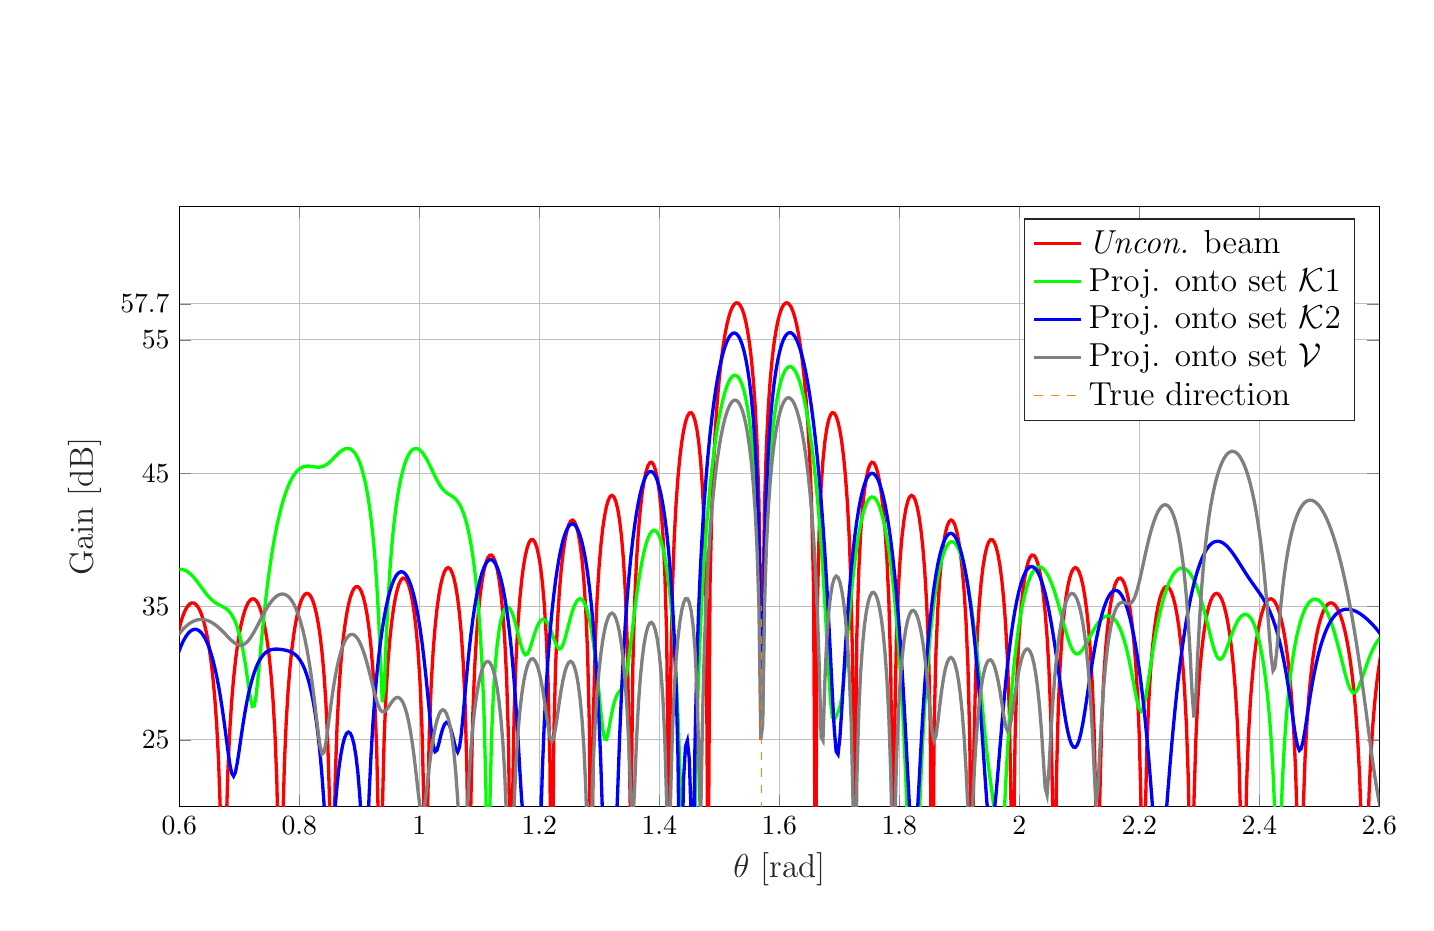
\begin{tikzpicture}

\begin{axis}[%
width=6in,
height=3in,
at={(0.758in,0.481in)},
scale only axis,
xmin=0.6,
xmax=2.6,
xlabel style={font=\large \color{white!15!black}},
xlabel={$\theta~[\mathrm{rad}]$},
ymin=20,
ymax=65,
ytick={25, 35, 45, 55, 57.7},
ylabel style={font=\large \color{white!15!black}},
ylabel={Gain~$[\mathrm{dB}]$},
xmajorgrids,
ymajorgrids,
axis background/.style={fill=white},
legend style={font=\large, legend cell align=left, align=left, draw=white!15!black}
]
\addplot [color=red, line width=1.2pt]
  table[row sep=crcr]{%
0.0031384541993904	34.8929512234198\\
0.00627690839878081	34.892846994354\\
0.00941536259817121	34.8926626310546\\
0.0125538167975616	34.8923821608349\\
0.015692270996952	34.8919832209524\\
0.0188307251963424	34.8914370571422\\
0.0219691793957328	34.8907085211087\\
0.0251076335951232	34.8897560664183\\
0.0282460877945136	34.8885317422337\\
0.031384541993904	34.8869811841477\\
0.0345229961932944	34.8850436012943\\
0.0376614503926848	34.8826517587886\\
0.0407999045920752	34.8797319544329\\
0.0439383587914656	34.8762039885127\\
0.047076812990856	34.8719811253595\\
0.0502152671902464	34.8669700452539\\
0.0533537213896369	34.8610707850904\\
0.0564921755890272	34.8541766660637\\
0.0596306297884176	34.8461742065106\\
0.0627690839878081	34.836943017828\\
0.0659075381871985	34.8263556812157\\
0.0690459923865889	34.8142776027844\\
0.0721844465859793	34.8005668443006\\
0.0753229007853697	34.7850739266045\\
0.0784613549847601	34.7676416023891\\
0.0815998091841505	34.7481045946957\\
0.0847382633835409	34.7262892970768\\
0.0878767175829313	34.7020134308821\\
0.0910151717823217	34.6750856545941\\
0.0941536259817121	34.6453051194984\\
0.0972920801811025	34.6124609652101\\
0.100430534380493	34.5763317477453\\
0.103568988579883	34.5366847917463\\
0.106707442779274	34.4932754573026\\
0.109845896978664	34.4458463103583\\
0.112984351178054	34.3941261840066\\
0.116122805377445	34.3378291159557\\
0.119261259576835	34.2766531450324\\
0.122399713776226	34.2102789467203\\
0.125538167975616	34.1383682842636\\
0.128676622175006	34.0605622476472\\
0.131815076374397	33.9764792477462\\
0.134953530573787	33.8857127267044\\
0.138091984773178	33.7878285380875\\
0.141230438972568	33.6823619410247\\
0.144368893171959	33.5688141410928\\
0.147507347371349	33.4466482963926\\
0.150645801570739	33.315284889408\\
0.15378425577013	33.1740963427517\\
0.15692270996952	33.022400728377\\
0.160061164168911	32.8594543834808\\
0.163199618368301	32.6844431994793\\
0.166338072567691	32.496472289739\\
0.169476526767082	32.2945536622953\\
0.172614980966472	32.0775914188372\\
0.175753435165863	31.844363861235\\
0.178891889365253	31.5935016979631\\
0.182030343564643	31.3234612850484\\
0.185168797764034	31.032491479762\\
0.188307251963424	30.7185921859304\\
0.191445706162815	30.3794619591991\\
0.194584160362205	30.0124310129442\\
0.197722614561595	29.6143744519519\\
0.200861068760986	29.1815982869752\\
0.203999522960376	28.7096872894338\\
0.207137977159767	28.1932982433929\\
0.210276431359157	27.6258732406337\\
0.213414885558547	26.999232767757\\
0.216553339757938	26.302982510563\\
0.219691793957328	25.5236211162388\\
0.222830248156719	24.643147500707\\
0.225968702356109	23.6367877902926\\
0.229107156555499	22.469076171157\\
0.23224561075489	21.0866132193838\\
0.23538406495428	19.4034188281667\\
0.238522519153671	17.2674005130353\\
0.241660973353061	14.3682275901092\\
0.244799427552451	9.89399832243571\\
0.247937881751842	-0.0348459594645641\\
0.251076335951232	1.57398720245486\\
0.254214790150623	10.5841540930961\\
0.257353244350013	14.9541574847176\\
0.260491698549403	17.8686756859255\\
0.263630152748794	20.0592129880311\\
0.266768606948184	21.8138322189111\\
0.269907061147575	23.2758461448407\\
0.273045515346965	24.5269580442147\\
0.276183969546355	25.6181437251214\\
0.279322423745746	26.5833206867292\\
0.282460877945136	27.446169894132\\
0.285599332144527	28.2238535405759\\
0.288737786343917	28.9291828771802\\
0.291876240543307	29.5719519536926\\
0.295014694742698	30.1597948030046\\
0.298153148942088	30.6987566432284\\
0.301291603141479	31.1936862637687\\
0.304430057340869	31.6485126245469\\
0.307568511540259	32.0664441805928\\
0.31070696573965	32.4501152495038\\
0.31384541993904	32.8016952197411\\
0.316983874138431	33.1229711208125\\
0.320122328337821	33.4154107150839\\
0.323260782537211	33.6802110749441\\
0.326399236736602	33.9183361408497\\
0.329537690935992	34.1305457523885\\
0.332676145135383	34.3174179437398\\
0.335814599334773	34.4793657946501\\
0.338953053534163	34.6166497615689\\
0.342091507733554	34.7293861370594\\
0.345229961932944	34.8175520686425\\
0.348368416132335	34.8809873892375\\
0.351506870331725	34.9193933539813\\
0.354645324531115	34.9323282287063\\
0.357783778730506	34.9191995214886\\
0.360922232929896	34.8792524770454\\
0.364060687129287	34.811554249196\\
0.367199141328677	34.7149729090414\\
0.370337595528067	34.5881501085822\\
0.373476049727458	34.4294657615905\\
0.376614503926848	34.2369924666236\\
0.379752958126239	34.0084364903711\\
0.382891412325629	33.7410608109354\\
0.38602986652502	33.4315837606324\\
0.38916832072441	33.0760438276551\\
0.3923067749238	32.6696165315153\\
0.395445229123191	32.2063618498528\\
0.398583683322581	31.6788683964155\\
0.401722137521972	31.0777395675833\\
0.404860591721362	30.3908295619111\\
0.407999045920752	29.6020676779218\\
0.411137500120143	28.6895725635333\\
0.414275954319533	27.6224707842243\\
0.417414408518924	26.3551795156403\\
0.420552862718314	24.8162613418211\\
0.423691316917704	22.8841914234003\\
0.426829771117095	20.3257922611977\\
0.429968225316485	16.5964106808631\\
0.433106679515876	9.80203388674862\\
0.436245133715266	-1.7872955375999\\
0.439383587914656	12.9581612312677\\
0.442522042114047	18.2686731158083\\
0.445660496313437	21.5379942452366\\
0.448798950512828	23.8931760435422\\
0.451937404712218	25.7234643476408\\
0.455075858911608	27.2097350038448\\
0.458214313110999	28.4507405444274\\
0.461352767310389	29.5062184523679\\
0.46449122150978	30.4149597323142\\
0.46762967570917	31.2034832521974\\
0.47076812990856	31.8906259902323\\
0.473906584107951	32.4901570972326\\
0.477045038307341	33.0123540639305\\
0.480183492506732	33.4649970264906\\
0.483321946706122	33.8540188508189\\
0.486460400905512	34.1839420110611\\
0.489598855104903	34.458177881712\\
0.492737309304293	34.6792337132155\\
0.495875763503684	34.8488551264152\\
0.499014217703074	34.9681214765388\\
0.502152671902464	35.0375048093376\\
0.505291126101855	35.0568986667889\\
0.508429580301245	35.0256197064174\\
0.511568034500636	34.942382334423\\
0.514706488700026	34.805243824772\\
0.517844942899416	34.6115142201717\\
0.520983397098807	34.3576210776952\\
0.524121851298197	34.0389129119363\\
0.527260305497588	33.6493754498999\\
0.530398759696978	33.1812187349126\\
0.533537213896368	32.6242653291338\\
0.536675668095759	31.9650195309584\\
0.539814122295149	31.1852014910699\\
0.54295257649454	30.259335461236\\
0.54609103069393	29.1505570667793\\
0.54922948489332	27.8027919449283\\
0.552367939092711	26.1247448355064\\
0.555506393292101	23.9526405203079\\
0.558644847491492	20.9453323165605\\
0.561783301690882	16.1767447373858\\
0.564921755890272	4.82595051473846\\
0.568060210089663	10.4058304527293\\
0.571198664289053	18.1910629523417\\
0.574337118488444	22.2318849347663\\
0.577475572687834	24.9500688764585\\
0.580614026887224	26.9787134016155\\
0.583752481086615	28.5777783959647\\
0.586890935286005	29.879258088738\\
0.590029389485396	30.9591740036202\\
0.593167843684786	31.8651047627285\\
0.596306297884177	32.6285960224688\\
0.599444752083567	33.2714275816352\\
0.602583206282957	33.8090520589761\\
0.605721660482348	34.2526025939754\\
0.608860114681738	34.6101202333085\\
0.611998568881128	34.8873279599812\\
0.615137023080519	35.0881254941322\\
0.618275477279909	35.2149013879558\\
0.6214139314793	35.2687166935709\\
0.62455238567869	35.249389568103\\
0.627690839878081	35.1554936983476\\
0.630829294077471	34.984270404937\\
0.633967748276861	34.7314412288873\\
0.637106202476252	34.3908912050064\\
0.640244656675642	33.9541678618635\\
0.643383110875033	33.4096982405385\\
0.646521565074423	32.7415475796615\\
0.649660019273813	31.927388230597\\
0.652798473473204	30.9350183857352\\
0.655936927672594	29.7160098577815\\
0.659075381871985	28.1931079185544\\
0.662213836071375	26.2322098853677\\
0.665352290270765	23.568812432299\\
0.668490744470156	19.5559741689573\\
0.671629198669546	11.6912190532504\\
0.674767652868937	6.94146000409802\\
0.677906107068327	17.9537798866446\\
0.681044561267717	22.6998595000353\\
0.684183015467108	25.7126064387521\\
0.687321469666498	27.8917661555839\\
0.690459923865889	29.5712138125174\\
0.693598378065279	30.911395267996\\
0.696736832264669	32.0014441411603\\
0.69987528646406	32.8956488531194\\
0.70301374066345	33.6291621648944\\
0.706152194862841	34.2256738923921\\
0.709290649062231	34.7015067984619\\
0.712429103261621	35.0679456562468\\
0.715567557461012	35.3326164653677\\
0.718706011660402	35.5003143011413\\
0.721844465859793	35.5734839383415\\
0.724982920059183	35.5524582924093\\
0.728121374258573	35.4355028573096\\
0.731259828457964	35.2186749429722\\
0.734398282657354	34.8954701935353\\
0.737536736856745	34.4561828670007\\
0.740675191056135	33.8868324519314\\
0.743813645255525	33.1673717493259\\
0.746952099454916	32.2686087297232\\
0.750090553654306	31.1466359644798\\
0.753229007853697	29.7319596332616\\
0.756367462053087	27.90592551877\\
0.759505916252478	25.4411960126928\\
0.762644370451868	21.8108782371099\\
0.765782824651258	15.2281952257448\\
0.768921278850649	3.13641302773942\\
0.772059733050039	17.8631239915564\\
0.775198187249429	23.2113834580099\\
0.77833664144882	26.4504530336619\\
0.78147509564821	28.7382019635788\\
0.784613549847601	30.4713406379844\\
0.787752004046991	31.8329030150391\\
0.790890458246381	32.9219351070474\\
0.794028912445772	33.7975500257441\\
0.797167366645162	34.4973013445652\\
0.800305820844553	35.0459428628088\\
0.803444275043943	35.4600058395585\\
0.806582729243334	35.7503384644633\\
0.809721183442724	35.9235524338068\\
0.812859637642114	35.9828235702162\\
0.815998091841505	35.9282615838413\\
0.819136546040895	35.7569399113734\\
0.822275000240286	35.4625929450413\\
0.825413454439676	35.0349074603027\\
0.828551908639066	34.4582224068002\\
0.831690362838457	33.7092480488982\\
0.834828817037847	32.7529890916488\\
0.837967271237237	31.5350514690707\\
0.841105725436628	29.9658322947139\\
0.844244179636018	27.8837252696265\\
0.847382633835409	24.9517896785555\\
0.850521088034799	20.2586268958812\\
0.85365954223419	9.1444485271695\\
0.85679799643358	14.2931193037801\\
0.85993645063297	22.1377132308637\\
0.863074904832361	26.1611892121205\\
0.866213359031751	28.8295901078495\\
0.869351813231142	30.7828005349423\\
0.872490267430532	32.2821948329478\\
0.875628721629922	33.4595857120364\\
0.878767175829313	34.3900350774152\\
0.881905630028703	35.1195931243934\\
0.885044084228094	35.6777287498891\\
0.888182538427484	36.0835287281626\\
0.891320992626874	36.3490020057323\\
0.894459446826265	36.4808798669732\\
0.897597901025655	36.4815370583261\\
0.900736355225046	36.3493129010163\\
0.903874809424436	36.078322786255\\
0.907013263623826	35.6577079528953\\
0.910151717823217	35.0701026876276\\
0.913290172022607	34.2888088656721\\
0.916428626221997	33.2725532075911\\
0.919567080421388	31.9551948526135\\
0.922705534620778	30.2234838925889\\
0.925843988820169	27.8614720375062\\
0.928982443019559	24.3755659500906\\
0.93212089721895	18.1480109398072\\
0.93525935141834	3.01873765051552\\
0.93839780561773	19.6255519745196\\
0.941536259817121	25.2179278257458\\
0.944674714016511	28.5276622110609\\
0.947813168215902	30.8296086954191\\
0.950951622415292	32.5459422445072\\
0.954090076614682	33.8680112762774\\
0.957228530814073	34.8978937345567\\
0.960366985013463	35.6955167542779\\
0.963505439212854	36.2980245065704\\
0.966643893412244	36.7288709987864\\
0.969782347611634	37.0024530133127\\
0.972920801811025	37.1265408296604\\
0.976059256010415	37.1034672663968\\
0.979197710209806	36.9304812349732\\
0.982336164409196	36.5993780473207\\
0.985474618608586	36.0952897819575\\
0.988613072807977	35.3942224212439\\
0.991751527007367	34.4583641703846\\
0.994889981206758	33.2268692785174\\
0.998028435406148	31.596189334398\\
1.00116688960554	29.3720652471347\\
1.00430534380493	26.1244765681409\\
1.00744379800432	20.5423367830299\\
1.01058225220371	3.19229377161532\\
1.0137207064031	19.5124032498942\\
1.01685916060249	25.7368711692008\\
1.01999761480188	29.2602388967241\\
1.02313606900127	31.6648711027801\\
1.02627452320066	33.436077183062\\
1.02941297740005	34.7862005122603\\
1.03255143159944	35.8260826663514\\
1.03568988579883	36.6197142750691\\
1.03882833999822	37.2060947362216\\
1.04196679419761	37.6092824639475\\
1.045105248397	37.843404020014\\
1.04824370259639	37.9151849881574\\
1.05138215679578	37.8250575392633\\
1.05452061099518	37.5672494932493\\
1.05765906519457	37.1288861767315\\
1.06079751939396	36.4877828117593\\
1.06393597359335	35.6080361192082\\
1.06707442779274	34.4312582676992\\
1.07021288199213	32.857881086978\\
1.07335133619152	30.7018678304183\\
1.07648979039091	27.5558747462077\\
1.0796282445903	22.2087825344637\\
1.08276669878969	5.92694912931209\\
1.08590515298908	20.1475863319946\\
1.08904360718847	26.6857473515411\\
1.09218206138786	30.3061234217213\\
1.09532051558725	32.7537450559651\\
1.09845896978664	34.5440769935904\\
1.10159742398603	35.89896286441\\
1.10473587818542	36.9329590158688\\
1.10787433238481	37.7115458859282\\
1.1110127865842	38.2741131368734\\
1.11415124078359	38.6444037402467\\
1.11728969498298	38.8356280911327\\
1.12042814918237	38.852937678211\\
1.12356660338176	38.6943285809307\\
1.12670505758115	38.3503242318137\\
1.12984351178054	37.8023179617131\\
1.13298196597994	37.0189033579101\\
1.13612042017933	35.9484499151874\\
1.13925887437872	34.5034580754401\\
1.14239732857811	32.523794366457\\
1.1455357827775	29.6728924485652\\
1.14867423697689	25.0335338812364\\
1.15181269117628	13.6951507375313\\
1.15495114537567	19.0003347829647\\
1.15808959957506	26.9608886939105\\
1.16122805377445	30.9882191930634\\
1.16436650797384	33.6309290033722\\
1.16750496217323	35.5355187448621\\
1.17064341637262	36.9639211446183\\
1.17378187057201	38.0469293553269\\
1.1769203247714	38.8576903337832\\
1.18005877897079	39.4394909618061\\
1.18319723317018	39.8180187990344\\
1.18633568736957	40.0072283041216\\
1.18947414156896	40.0121021380377\\
1.19261259576835	39.8295751335462\\
1.19575104996774	39.4480007364416\\
1.19888950416713	38.8449440353582\\
1.20202795836652	37.9823267372174\\
1.20516641256591	36.7963616753682\\
1.20830486676531	35.1753720199125\\
1.2114433209647	32.9038828282505\\
1.21458177516409	29.4854144608262\\
1.21772022936348	23.2694518354499\\
1.22085868356287	5.83549290361533\\
1.22399713776226	24.8477662578215\\
1.22713559196165	30.4782743565734\\
1.23027404616104	33.7879824520801\\
1.23341250036043	36.06970455298\\
1.23655095455982	37.7471455831803\\
1.23968940875921	39.0109869278378\\
1.2428278629586	39.9617730417789\\
1.24596631715799	40.6571683633166\\
1.24910477135738	41.1311950128701\\
1.25224322555677	41.4030417275967\\
1.25538167975616	41.4812289203132\\
1.25852013395555	41.3652811409643\\
1.26165858815494	41.0456514783001\\
1.26479704235433	40.5018661415863\\
1.26793549655372	39.6980559693983\\
1.27107395075311	38.573524940995\\
1.2742124049525	37.0219964835552\\
1.27735085915189	34.8398708833831\\
1.28048931335128	31.5656606539295\\
1.28362776755067	25.7243018411309\\
1.28676622175007	3.28876539954894\\
1.28990467594946	26.0109333039082\\
1.29304313014885	31.9814573114136\\
1.29618158434824	35.4189860058402\\
1.29932003854763	37.7723098973527\\
1.30245849274702	39.4973288848972\\
1.30559694694641	40.7954968479535\\
1.3087354011458	41.7718728100005\\
1.31187385534519	42.4862071852826\\
1.31501230954458	42.9734407796414\\
1.31815076374397	43.2529824332241\\
1.32128921794336	43.3330276464366\\
1.32442767214275	43.2122087887118\\
1.32756612634214	42.8793340081648\\
1.33070458054153	42.3110998743061\\
1.33384303474092	41.4666956303538\\
1.33698148894031	40.2762624788923\\
1.3401199431397	38.6147196489325\\
1.34325839733909	36.2331771887701\\
1.34639685153848	32.5269056446761\\
1.34953530573787	25.2031355867997\\
1.35267375993726	17.1920328089721\\
1.35581221413665	30.3429821463429\\
1.35895066833604	35.3619549301961\\
1.36208912253543	38.458410000597\\
1.36522757673483	40.6379905335335\\
1.36836603093422	42.25791538033\\
1.37150448513361	43.4849702648383\\
1.374642939333	44.4086678238327\\
1.37778139353239	45.0804826792778\\
1.38091984773178	45.5302243314088\\
1.38405830193117	45.7735516719531\\
1.38719675613056	45.8153549795733\\
1.39033521032995	45.6507265567632\\
1.39347366452934	45.2639623590877\\
1.39661211872873	44.6251388318729\\
1.39975057292812	43.6825181711204\\
1.40288902712751	42.3459865370028\\
1.4060274813269	40.4472816420406\\
1.40916593552629	37.6248450457488\\
1.41230438972568	32.8540855266063\\
1.41544284392507	19.5824961638675\\
1.41858129812446	28.54145103323\\
1.42171975232385	36.0800167181305\\
1.42485820652324	40.0599648964796\\
1.42799666072263	42.729099979661\\
1.43113511492202	44.6846960913204\\
1.43427356912141	46.1734427053108\\
1.4374120233208	47.3196148523086\\
1.44055047752019	48.1927654454487\\
1.44368893171959	48.8336102665068\\
1.44682738591898	49.2654497578748\\
1.44996584011837	49.4995003307501\\
1.45310429431776	49.537129979947\\
1.45624274851715	49.3700555962041\\
1.45938120271654	48.9785871525106\\
1.46251965691593	48.3271023444389\\
1.46565811111532	47.3543110581976\\
1.46879656531471	45.9515955331617\\
1.4719350195141	43.9083812402377\\
1.47507347371349	40.7395690505915\\
1.47821192791288	34.8403653440559\\
1.48135038211227	11.6045611224286\\
1.48448883631166	36.4416175572715\\
1.48762729051105	42.4407696121813\\
1.49076574471044	46.0497388889833\\
1.49390419890983	48.625534144798\\
1.49704265310922	50.6065461877332\\
1.50018110730861	52.1905145236025\\
1.503319561508	53.4833983238501\\
1.50645801570739	54.5482824822571\\
1.50959646990678	55.4253899958286\\
1.51273492410617	56.141515608661\\
1.51587337830556	56.7149289254334\\
1.51901183250496	57.1581001968617\\
1.52215028670435	57.4792771162726\\
1.52528874090374	57.683400159692\\
1.52842719510313	57.772598041486\\
1.53156564930252	57.7463797971894\\
1.53470410350191	57.6015655192873\\
1.5378425577013	57.3319400381606\\
1.54098101190069	56.9275499059855\\
1.54411946610008	56.3734670080263\\
1.54725792029947	55.6476625106701\\
1.55039637449886	54.7172580036849\\
1.55353482869825	53.5315417450898\\
1.55667328289764	52.0078321598104\\
1.55981173709703	49.99923475191\\
1.56295019129642	47.2067381393144\\
1.56608864549581	42.8561648618556\\
1.5692270996952	33.3568491370331\\
1.57236555389459	33.3568491370331\\
1.57550400809398	42.8561648618556\\
1.57864246229337	47.2067381393144\\
1.58178091649276	49.99923475191\\
1.58491937069215	52.0078321598104\\
1.58805782489154	53.5315417450899\\
1.59119627909093	54.7172580036849\\
1.59433473329032	55.6476625106701\\
1.59747318748972	56.3734670080263\\
1.60061164168911	56.9275499059856\\
1.6037500958885	57.3319400381606\\
1.60688855008789	57.6015655192873\\
1.61002700428728	57.7463797971894\\
1.61316545848667	57.772598041486\\
1.61630391268606	57.683400159692\\
1.61944236688545	57.4792771162726\\
1.62258082108484	57.1581001968617\\
1.62571927528423	56.7149289254334\\
1.62885772948362	56.141515608661\\
1.63199618368301	55.4253899958287\\
1.6351346378824	54.5482824822571\\
1.63827309208179	53.4833983238502\\
1.64141154628118	52.1905145236025\\
1.64455000048057	50.6065461877332\\
1.64768845467996	48.625534144798\\
1.65082690887935	46.0497388889831\\
1.65396536307874	42.4407696121816\\
1.65710381727813	36.4416175572711\\
1.66024227147752	11.6045611224214\\
1.66338072567691	34.8403653440565\\
1.6665191798763	40.7395690505912\\
1.66965763407569	43.908381240238\\
1.67279608827508	45.9515955331617\\
1.67593454247447	47.3543110581976\\
1.67907299667387	48.327102344439\\
1.68221145087326	48.9785871525106\\
1.68534990507265	49.3700555962042\\
1.68848835927204	49.537129979947\\
1.69162681347143	49.4995003307501\\
1.69476526767082	49.2654497578748\\
1.69790372187021	48.8336102665068\\
1.7010421760696	48.1927654454487\\
1.70418063026899	47.3196148523085\\
1.70731908446838	46.1734427053108\\
1.71045753866777	44.6846960913205\\
1.71359599286716	42.7290999796608\\
1.71673444706655	40.0599648964799\\
1.71987290126594	36.0800167181294\\
1.72301135546533	28.5414510332294\\
1.72614980966472	19.5824961638666\\
1.72928826386411	32.8540855266063\\
1.7324267180635	37.6248450457488\\
1.73556517226289	40.4472816420406\\
1.73870362646228	42.3459865370028\\
1.74184208066167	43.6825181711204\\
1.74498053486106	44.6251388318727\\
1.74811898906045	45.2639623590875\\
1.75125744325984	45.6507265567632\\
1.75439589745924	45.8153549795733\\
1.75753435165863	45.7735516719531\\
1.76067280585802	45.5302243314088\\
1.76381126005741	45.0804826792779\\
1.7669497142568	44.4086678238327\\
1.77008816845619	43.4849702648384\\
1.77322662265558	42.2579153803304\\
1.77636507685497	40.6379905335332\\
1.77950353105436	38.458410000597\\
1.78264198525375	35.3619549301961\\
1.78578043945314	30.3429821463431\\
1.78891889365253	17.192032808972\\
1.79205734785192	25.2031355868004\\
1.79519580205131	32.5269056446756\\
1.7983342562507	36.2331771887701\\
1.80147271045009	38.6147196489323\\
1.80461116464948	40.2762624788925\\
1.80774961884887	41.4666956303538\\
1.81088807304826	42.311099874306\\
1.81402652724765	42.8793340081648\\
1.81716498144704	43.2122087887118\\
1.82030343564643	43.3330276464366\\
1.82344188984582	43.2529824332242\\
1.82658034404521	42.9734407796415\\
1.8297187982446	42.4862071852828\\
1.83285725244399	41.7718728100007\\
1.83599570664339	40.795496847953\\
1.83913416084278	39.4973288848971\\
1.84227261504217	37.7723098973533\\
1.84541106924156	35.4189860058403\\
1.84854952344095	31.981457311414\\
1.85168797764034	26.0109333039079\\
1.85482643183973	3.28876539954982\\
1.85796488603912	25.7243018411308\\
1.86110334023851	31.5656606539295\\
1.8642417944379	34.8398708833832\\
1.86738024863729	37.0219964835551\\
1.87051870283668	38.573524940995\\
1.87365715703607	39.6980559693984\\
1.87679561123546	40.5018661415866\\
1.87993406543485	41.0456514783005\\
1.88307251963424	41.3652811409642\\
1.88621097383363	41.481228920313\\
1.88934942803302	41.4030417275968\\
1.89248788223241	41.1311950128701\\
1.8956263364318	40.6571683633168\\
1.89876479063119	39.9617730417787\\
1.90190324483058	39.0109869278379\\
1.90504169902997	37.7471455831803\\
1.90818015322936	36.0697045529793\\
1.91131860742876	33.7879824520803\\
1.91445706162815	30.4782743565724\\
1.91759551582754	24.8477662578211\\
1.92073397002693	5.83549290360382\\
1.92387242422632	23.2694518354487\\
1.92701087842571	29.4854144608266\\
1.9301493326251	32.9038828282506\\
1.93328778682449	35.1753720199127\\
1.93642624102388	36.7963616753682\\
1.93956469522327	37.982326737217\\
1.94270314942266	38.8449440353586\\
1.94584160362205	39.4480007364411\\
1.94898005782144	39.8295751335465\\
1.95211851202083	40.0121021380376\\
1.95525696622022	40.0072283041218\\
1.95839542041961	39.8180187990343\\
1.961533874619	39.4394909618062\\
1.96467232881839	38.8576903337826\\
1.96781078301778	38.0469293553271\\
1.97094923721717	36.9639211446183\\
1.97408769141656	35.5355187448615\\
1.97722614561595	33.6309290033731\\
1.98036459981534	30.988219193064\\
1.98350305401473	26.9608886939105\\
1.98664150821412	19.0003347829646\\
1.98977996241352	13.6951507375245\\
1.99291841661291	25.0335338812366\\
1.9960568708123	29.6728924485652\\
1.99919532501169	32.5237943664571\\
2.00233377921108	34.5034580754404\\
2.00547223341047	35.9484499151873\\
2.00861068760986	37.0189033579101\\
2.01174914180925	37.8023179617134\\
2.01488759600864	38.3503242318139\\
2.01802605020803	38.6943285809307\\
2.02116450440742	38.8529376782113\\
2.02430295860681	38.8356280911329\\
2.0274414128062	38.644403740246\\
2.03057986700559	38.274113136873\\
2.03371832120498	37.7115458859282\\
2.03685677540437	36.9329590158688\\
2.03999522960376	35.8989628644091\\
2.04313368380315	34.5440769935902\\
2.04627213800254	32.7537450559653\\
2.04941059220193	30.3061234217194\\
2.05254904640132	26.6857473515406\\
2.05568750060071	20.1475863320004\\
2.0588259548001	5.92694912930968\\
2.06196440899949	22.2087825344688\\
2.06510286319888	27.5558747462077\\
2.06824131739828	30.7018678304182\\
2.07137977159767	32.8578810869779\\
2.07451822579706	34.4312582676995\\
2.07765667999645	35.608036119208\\
2.08079513419584	36.4877828117586\\
2.08393358839523	37.1288861767316\\
2.08707204259462	37.5672494932489\\
2.09021049679401	37.8250575392636\\
2.0933489509934	37.9151849881575\\
2.09648740519279	37.843404020014\\
2.09962585939218	37.6092824639474\\
2.10276431359157	37.2060947362214\\
2.10590276779096	36.619714275069\\
2.10904122199035	35.8260826663515\\
2.11217967618974	34.786200512261\\
2.11531813038913	33.4360771830622\\
2.11845658458852	31.6648711027794\\
2.12159503878791	29.2602388967243\\
2.1247334929873	25.7368711692009\\
2.12787194718669	19.512403249895\\
2.13101040138608	3.19229377160858\\
2.13414885558547	20.5423367830313\\
2.13728730978486	26.1244765681411\\
2.14042576398425	29.3720652471347\\
2.14356421818364	31.5961893343979\\
2.14670267238304	33.2268692785174\\
2.14984112658243	34.4583641703846\\
2.15297958078182	35.3942224212423\\
2.15611803498121	36.0952897819575\\
2.1592564891806	36.5993780473207\\
2.16239494337999	36.9304812349732\\
2.16553339757938	37.1034672663973\\
2.16867185177877	37.1265408296605\\
2.17181030597816	37.0024530133127\\
2.17494876017755	36.7288709987864\\
2.17808721437694	36.2980245065702\\
2.18122566857633	35.6955167542773\\
2.18436412277572	34.8978937345565\\
2.18750257697511	33.8680112762778\\
2.1906410311745	32.5459422445067\\
2.19377948537389	30.8296086954192\\
2.19691793957328	28.5276622110616\\
2.20005639377267	25.2179278257458\\
2.20319484797206	19.6255519745141\\
2.20633330217145	3.01873765051481\\
2.20947175637084	18.1480109398061\\
2.21261021057023	24.3755659500915\\
2.21574866476962	27.8614720375066\\
2.21888711896901	30.2234838925893\\
2.22202557316841	31.9551948526136\\
2.2251640273678	33.2725532075908\\
2.22830248156719	34.2888088656723\\
2.23144093576658	35.0701026876282\\
2.23457938996597	35.6577079528954\\
2.23771784416536	36.0783227862551\\
2.24085629836475	36.3493129010164\\
2.24399475256414	36.4815370583257\\
2.24713320676353	36.4808798669733\\
2.25027166096292	36.3490020057322\\
2.25341011516231	36.0835287281628\\
2.2565485693617	35.6777287498891\\
2.25968702356109	35.1195931243934\\
2.26282547776048	34.3900350774154\\
2.26596393195987	33.4595857120363\\
2.26910238615926	32.2821948329478\\
2.27224084035865	30.7828005349426\\
2.27537929455804	28.8295901078494\\
2.27851774875743	26.1611892121196\\
2.28165620295682	22.1377132308628\\
2.28479465715621	14.2931193037812\\
2.2879331113556	9.14444852716938\\
2.29107156555499	20.2586268958808\\
2.29421001975438	24.951789678556\\
2.29734847395377	27.8837252696261\\
2.30048692815316	29.9658322947138\\
2.30362538235256	31.5350514690716\\
2.30676383655195	32.7529890916487\\
2.30990229075134	33.709248048898\\
2.31304074495073	34.4582224068001\\
2.31617919915012	35.034907460303\\
2.31931765334951	35.4625929450412\\
2.3224561075489	35.7569399113739\\
2.32559456174829	35.9282615838416\\
2.32873301594768	35.9828235702163\\
2.33187147014707	35.9235524338071\\
2.33500992434646	35.7503384644644\\
2.33814837854585	35.4600058395584\\
2.34128683274524	35.0459428628091\\
2.34442528694463	34.4973013445653\\
2.34756374114402	33.7975500257441\\
2.35070219534341	32.9219351070477\\
2.3538406495428	31.832903015039\\
2.35697910374219	30.4713406379857\\
2.36011755794158	28.7382019635788\\
2.36325601214097	26.4504530336616\\
2.36639446634036	23.2113834580091\\
2.36953292053975	17.863123991558\\
2.37267137473914	3.13641302773091\\
2.37580982893853	15.2281952257434\\
2.37894828313792	21.8108782371068\\
2.38208673733732	25.4411960126935\\
2.38522519153671	27.9059255187693\\
2.3883636457361	29.7319596332622\\
2.39150209993549	31.1466359644799\\
2.39464055413488	32.2686087297232\\
2.39777900833427	33.1673717493263\\
2.40091746253366	33.8868324519312\\
2.40405591673305	34.4561828670008\\
2.40719437093244	34.8954701935352\\
2.41033282513183	35.218674942973\\
2.41347127933122	35.4355028573096\\
2.41660973353061	35.5524582924091\\
2.41974818773	35.5734839383413\\
2.42288664192939	35.5003143011412\\
2.42602509612878	35.3326164653678\\
2.42916355032817	35.0679456562459\\
2.43230200452756	34.7015067984616\\
2.43544045872695	34.2256738923919\\
2.43857891292634	33.6291621648949\\
2.44171736712573	32.8956488531188\\
2.44485582132512	32.0014441411603\\
2.44799427552451	30.9113952679966\\
2.4511327297239	29.5712138125179\\
2.4542711839233	27.8917661555843\\
2.45740963812269	25.7126064387513\\
2.46054809232208	22.6998595000364\\
2.46368654652147	17.9537798866459\\
2.46682500072086	6.94146000408388\\
2.46996345492025	11.6912190532487\\
2.47310190911964	19.5559741689568\\
2.47624036331903	23.5688124322981\\
2.47937881751842	26.2322098853671\\
2.48251727171781	28.1931079185536\\
2.4856557259172	29.7160098577806\\
2.48879418011659	30.935018385736\\
2.49193263431598	31.9273882305972\\
2.49507108851537	32.7415475796615\\
2.49820954271476	33.4096982405381\\
2.50134799691415	33.9541678618635\\
2.50448645111354	34.3908912050063\\
2.50762490531293	34.7314412288873\\
2.51076335951232	34.9842704049371\\
2.51390181371171	35.1554936983473\\
2.5170402679111	35.249389568103\\
2.52017872211049	35.2687166935709\\
2.52331717630988	35.2149013879555\\
2.52645563050927	35.0881254941323\\
2.52959408470866	34.887327959981\\
2.53273253890806	34.6101202333094\\
2.53587099310745	34.2526025939752\\
2.53900944730684	33.8090520589768\\
2.54214790150623	33.2714275816349\\
2.54528635570562	32.6285960224686\\
2.54842480990501	31.865104762729\\
2.5515632641044	30.9591740036199\\
2.55470171830379	29.8792580887385\\
2.55784017250318	28.5777783959654\\
2.56097862670257	26.9787134016157\\
2.56411708090196	24.9500688764591\\
2.56725553510135	22.2318849347638\\
2.57039398930074	18.1910629523434\\
2.57353244350013	10.405830452719\\
2.57667089769952	4.8259505147512\\
2.57980935189891	16.1767447373884\\
2.5829478060983	20.9453323165605\\
2.58608626029769	23.9526405203073\\
2.58922471449708	26.1247448355072\\
2.59236316869647	27.802791944929\\
2.59550162289586	29.150557066779\\
2.59864007709525	30.2593354612359\\
2.60177853129464	31.1852014910699\\
2.60491698549403	31.9650195309583\\
2.60805543969342	32.6242653291338\\
2.61119389389282	33.1812187349124\\
2.61433234809221	33.6493754498999\\
2.6174708022916	34.0389129119363\\
2.62060925649099	34.357621077695\\
2.62374771069038	34.6115142201721\\
2.62688616488977	34.8052438247721\\
2.63002461908916	34.9423823344224\\
2.63316307328855	35.0256197064174\\
2.63630152748794	35.0568986667888\\
2.63943998168733	35.0375048093374\\
2.64257843588672	34.9681214765388\\
2.64571689008611	34.8488551264149\\
2.6488553442855	34.6792337132153\\
2.65199379848489	34.4581778817119\\
2.65513225268428	34.1839420110608\\
2.65827070688367	33.8540188508185\\
2.66140916108306	33.4649970264904\\
2.66454761528245	33.0123540639297\\
2.66768606948184	32.4901570972318\\
2.67082452368123	31.8906259902317\\
2.67396297788062	31.2034832521969\\
2.67710143208001	30.4149597323138\\
2.6802398862794	29.5062184523681\\
2.68337834047879	28.4507405444268\\
2.68651679467818	27.2097350038463\\
2.68965524887758	25.7234643476407\\
2.69279370307697	23.8931760435415\\
2.69593215727636	21.5379942452369\\
2.69907061147575	18.2686731158081\\
2.70220906567514	12.9581612312625\\
2.70534751987453	-1.78729553761765\\
2.70848597407392	9.80203388675319\\
2.71162442827331	16.5964106808632\\
2.7147628824727	20.3257922611947\\
2.71790133667209	22.8841914234005\\
2.72103979087148	24.8162613418221\\
2.72417824507087	26.3551795156404\\
2.72731669927026	27.6224707842252\\
2.73045515346965	28.6895725635342\\
2.73359360766904	29.6020676779234\\
2.73673206186843	30.3908295619111\\
2.73987051606782	31.0777395675836\\
2.74300897026721	31.6788683964157\\
2.7461474244666	32.2063618498529\\
2.74928587866599	32.6696165315152\\
2.75242433286538	33.0760438276549\\
2.75556278706477	33.4315837606326\\
2.75870124126416	33.7410608109352\\
2.76183969546355	34.0084364903713\\
2.76497814966294	34.2369924666234\\
2.76811660386234	34.4294657615908\\
2.77125505806173	34.5881501085821\\
2.77439351226112	34.7149729090414\\
2.77753196646051	34.8115542491957\\
2.7806704206599	34.8792524770453\\
2.78380887485929	34.9191995214887\\
2.78694732905868	34.9323282287071\\
2.79008578325807	34.9193933539816\\
2.79322423745746	34.8809873892382\\
2.79636269165685	34.8175520686424\\
2.79950114585624	34.7293861370594\\
2.80263960005563	34.6166497615689\\
2.80577805425502	34.4793657946502\\
2.80891650845441	34.3174179437402\\
2.8120549626538	34.1305457523884\\
2.81519341685319	33.9183361408497\\
2.81833187105258	33.680211074944\\
2.82147032525197	33.4154107150839\\
2.82460877945136	33.1229711208118\\
2.82774723365075	32.801695219741\\
2.83088568785014	32.4501152495045\\
2.83402414204953	32.066444180593\\
2.83716259624892	31.6485126245472\\
2.84030105044831	31.1936862637688\\
2.84343950464771	30.6987566432286\\
2.8465779588471	30.159794803004\\
2.84971641304649	29.5719519536918\\
2.85285486724588	28.9291828771796\\
2.85599332144527	28.2238535405763\\
2.85913177564466	27.4461698941315\\
2.86227022984405	26.5833206867295\\
2.86540868404344	25.6181437251215\\
2.86854713824283	24.5269580442135\\
2.87168559244222	23.2758461448407\\
2.87482404664161	21.8138322189098\\
2.877962500841	20.059212988028\\
2.88110095504039	17.8686756859229\\
2.88423940923978	14.9541574847168\\
2.88737786343917	10.5841540930913\\
2.89051631763856	1.57398720244404\\
2.89365477183795	-0.0348459594175594\\
2.89679322603734	9.89399832244036\\
2.89993168023673	14.368227590109\\
2.90307013443612	17.2674005130374\\
2.90620858863551	19.4034188281644\\
2.9093470428349	21.0866132193863\\
2.91248549703429	22.4690761711568\\
2.91562395123368	23.6367877902925\\
2.91876240543307	24.6431475007074\\
2.92190085963247	25.5236211162391\\
2.92503931383186	26.3029825105638\\
2.92817776803125	26.9992327677569\\
2.93131622223064	27.6258732406325\\
2.93445467643003	28.1932982433942\\
2.93759313062942	28.7096872894356\\
2.94073158482881	29.1815982869748\\
2.9438700390282	29.6143744519524\\
2.94700849322759	30.0124310129451\\
2.95014694742698	30.3794619591993\\
2.95328540162637	30.7185921859312\\
2.95642385582576	31.0324914797624\\
2.95956231002515	31.3234612850485\\
2.96270076422454	31.5935016979634\\
2.96583921842393	31.8443638612349\\
2.96897767262332	32.0775914188379\\
2.97211612682271	32.2945536622954\\
2.9752545810221	32.4964722897395\\
2.97839303522149	32.6844431994795\\
2.98153148942088	32.8594543834813\\
2.98466994362027	33.0224007283771\\
2.98780839781966	33.1740963427521\\
2.99094685201905	33.3152848894083\\
2.99408530621844	33.4466482963925\\
2.99722376041783	33.5688141410928\\
3.00036221461722	33.6823619410249\\
3.00350066881662	33.7878285380873\\
3.00663912301601	33.8857127267045\\
3.0097775772154	33.9764792477462\\
3.01291603141479	34.0605622476479\\
3.01605448561418	34.1383682842639\\
3.01919293981357	34.2102789467205\\
3.02233139401296	34.2766531450326\\
3.02546984821235	34.3378291159561\\
3.02860830241174	34.3941261840078\\
3.03174675661113	34.4458463103584\\
3.03488521081052	34.4932754573028\\
3.03802366500991	34.5366847917469\\
3.0411621192093	34.5763317477455\\
3.04430057340869	34.61246096521\\
3.04743902760808	34.6453051194987\\
3.05057748180747	34.6750856545942\\
3.05371593600686	34.7020134308825\\
3.05685439020625	34.7262892970767\\
3.05999284440564	34.748104594696\\
3.06313129860503	34.7676416023895\\
3.06626975280442	34.7850739266047\\
3.06940820700381	34.8005668443006\\
3.0725466612032	34.8142776027849\\
3.07568511540259	34.8263556812161\\
3.07882356960198	34.8369430178283\\
3.08196202380138	34.8461742065107\\
3.08510047800077	34.8541766660639\\
3.08823893220016	34.8610707850905\\
3.09137738639955	34.8669700452542\\
3.09451584059894	34.8719811253596\\
3.09765429479833	34.876203988513\\
3.10079274899772	34.8797319544332\\
3.10393120319711	34.8826517587887\\
3.1070696573965	34.8850436012945\\
3.11020811159589	34.886981184148\\
3.11334656579528	34.888531742234\\
3.11648501999467	34.8897560664185\\
3.11962347419406	34.8907085211088\\
3.12276192839345	34.8914370571425\\
3.12590038259284	34.8919832209525\\
3.12903883679223	34.8923821608355\\
3.13217729099162	34.8926626310547\\
3.13531574519101	34.892846994354\\
3.1384541993904	34.8929512234199\\
};
\addlegendentry{\emph{Uncon.} beam}


\addplot [color=green, line width=1.2pt]
  table[row sep=crcr]{%
0.0031384541993904	27.4371946765552\\
0.00627690839878081	27.4340026620587\\
0.00941536259817121	27.4286787292323\\
0.0125538167975616	27.4212170302074\\
0.015692270996952	27.411609408828\\
0.0188307251963424	27.399845432854\\
0.0219691793957328	27.3859124374002\\
0.0251076335951232	27.3697955810298\\
0.0282460877945136	27.3514779165135\\
0.031384541993904	27.3309404785598\\
0.0345229961932944	27.3081623913386\\
0.0376614503926848	27.283120999074\\
0.0407999045920752	27.2557920236418\\
0.0439383587914656	27.2261497536512\\
0.047076812990856	27.1941672702177\\
0.0502152671902464	27.159816715438\\
0.0533537213896369	27.1230696104735\\
0.0564921755890272	27.0838972310884\\
0.0596306297884176	27.0422710496841\\
0.0627690839878081	26.9981632540291\\
0.0659075381871985	26.9515473543604\\
0.0690459923865889	26.902398892025\\
0.0721844465859793	26.8506962645421\\
0.0753229007853697	26.7964216838584\\
0.0784613549847601	26.7395622865345\\
0.0815998091841505	26.6801114167577\\
0.0847382633835409	26.6180701053558\\
0.0878767175829313	26.5534487701235\\
0.0910151717823217	26.4862691650617\\
0.0941536259817121	26.4165666080135\\
0.0972920801811025	26.3443925176441\\
0.100430534380493	26.2698172916808\\
0.103568988579883	26.1929335577034\\
0.106707442779274	26.1138598260641\\
0.109845896978664	26.0327445699981\\
0.112984351178054	25.9497707505671\\
0.116122805377445	25.8651607922065\\
0.119261259576835	25.779181997204\\
0.122399713776226	25.6921523629495\\
0.125538167975616	25.6044467323235\\
0.128676622175006	25.5165031636756\\
0.131815076374397	25.4288293506996\\
0.134953530573787	25.3420088531005\\
0.138091984773178	25.25670681617\\
0.141230438972568	25.1736747627343\\
0.144368893171959	25.0937539387529\\
0.147507347371349	25.0178765914668\\
0.150645801570739	24.9470644691314\\
0.15378425577013	24.8824237709175\\
0.15692270996952	24.8251357673837\\
0.160061164168911	24.7764423819526\\
0.163199618368301	24.7376261981075\\
0.166338072567691	24.70998465717\\
0.169476526767082	24.6947986443601\\
0.172614980966472	24.6932962133223\\
0.175753435165863	24.7066128278049\\
0.178891889365253	24.7357501292168\\
0.182030343564643	24.78153576978\\
0.185168797764034	24.8445871711587\\
0.188307251963424	24.9252820812161\\
0.191445706162815	25.0237384505075\\
0.194584160362205	25.1398054451967\\
0.197722614561595	25.2730664350178\\
0.200861068760986	25.4228536870207\\
0.203999522960376	25.588273429513\\
0.207137977159767	25.7682390899789\\
0.210276431359157	25.961509970305\\
0.213414885558547	26.1667324503007\\
0.216553339757938	26.3824809814731\\
0.219691793957328	26.6072965684289\\
0.222830248156719	26.8397210279212\\
0.225968702356109	27.0783259559839\\
0.229107156555499	27.3217359330829\\
0.23224561075489	27.5686459955794\\
0.23538406495428	27.8178337710826\\
0.238522519153671	28.0681669128829\\
0.241660973353061	28.3186065898261\\
0.244799427552451	28.5682078171005\\
0.247937881751842	28.8161173771634\\
0.251076335951232	29.061570003042\\
0.254214790150623	29.3038833987855\\
0.257353244350013	29.5424525684251\\
0.260491698549403	29.77674382581\\
0.263630152748794	30.0062887685537\\
0.266768606948184	30.2306784231437\\
0.269907061147575	30.4495577054272\\
0.273045515346965	30.6626202908215\\
0.276183969546355	30.8696039499207\\
0.279322423745746	31.0702863763037\\
0.282460877945136	31.2644815124096\\
0.285599332144527	31.4520363644915\\
0.288737786343917	31.6328282878055\\
0.291876240543307	31.8067627167703\\
0.295014694742698	31.97377131096\\
0.298153148942088	32.1338104856411\\
0.301291603141479	32.2868602944305\\
0.304430057340869	32.4329236309858\\
0.307568511540259	32.5720257161689\\
0.31070696573965	32.7042138362361\\
0.31384541993904	32.8295572964341\\
0.316983874138431	32.9481475523345\\
0.320122328337821	33.0600984784894\\
0.323260782537211	33.1655467302006\\
0.326399236736602	33.2646521495713\\
0.329537690935992	33.3575981612978\\
0.332676145135383	33.4445920972948\\
0.335814599334773	33.5258653821211\\
0.338953053534163	33.6016735039459\\
0.342091507733554	33.6722956886089\\
0.345229961932944	33.7380341881984\\
0.348368416132335	33.7992130909597\\
0.351506870331725	33.8561765575655\\
0.354645324531115	33.9092863906693\\
0.357783778730506	33.9589188516872\\
0.360922232929896	34.0054606519108\\
0.364060687129287	34.0493040654384\\
0.367199141328677	34.0908411397884\\
0.370337595528067	34.130457016379\\
0.373476049727458	34.1685224169686\\
0.376614503926848	34.2053854017909\\
0.379752958126239	34.2413625582125\\
0.382891412325629	34.2767298313282\\
0.38602986652502	34.3117132557409\\
0.38916832072441	34.3464798857458\\
0.3923067749238	34.3811292443583\\
0.395445229123191	34.4156856158787\\
0.398583683322581	34.4500914892401\\
0.401722137521972	34.4842024194243\\
0.404860591721362	34.5177835134875\\
0.407999045920752	34.5505076702336\\
0.411137500120143	34.5819556146125\\
0.414275954319533	34.6116176771102\\
0.417414408518924	34.6388971829009\\
0.420552862718314	34.6631152431348\\
0.423691316917704	34.6835166876315\\
0.426829771117095	34.6992768489187\\
0.429968225316485	34.7095089041152\\
0.433106679515876	34.7132715037304\\
0.436245133715266	34.7095764637595\\
0.439383587914656	34.6973963674393\\
0.442522042114047	34.6756720139179\\
0.445660496313437	34.6433197625407\\
0.448798950512828	34.5992389552169\\
0.451937404712218	34.5423197606182\\
0.455075858911608	34.4714519823622\\
0.458214313110999	34.3855356239877\\
0.461352767310389	34.2834943284987\\
0.46449122150978	34.1642932400042\\
0.46762967570917	34.0269634096568\\
0.47076812990856	33.8706356377236\\
0.473906584107951	33.6945876649472\\
0.477045038307341	33.4983099524885\\
0.480183492506732	33.2815969422129\\
0.483321946706122	33.0446725973444\\
0.486460400905512	32.7883608997692\\
0.489598855104903	32.5143130866403\\
0.492737309304293	32.2253021585181\\
0.495875763503684	31.9255885686309\\
0.499014217703074	31.6213439656518\\
0.502152671902464	31.3210854237029\\
0.505291126101855	31.0360143738789\\
0.508429580301245	30.7800748330275\\
0.511568034500636	30.5694716619202\\
0.514706488700026	30.4213902866546\\
0.517844942899416	30.3518336445119\\
0.520983397098807	30.3728865541074\\
0.524121851298197	30.4901889003814\\
0.527260305497588	30.7015909281239\\
0.530398759696978	30.9975855362\\
0.533537213896368	31.3633203954998\\
0.536675668095759	31.781342092084\\
0.539814122295149	32.2341295357246\\
0.54295257649454	32.7058479758473\\
0.54609103069393	33.1832238910265\\
0.54922948489332	33.6557347247949\\
0.552367939092711	34.115387819165\\
0.555506393292101	34.5563169890025\\
0.558644847491492	34.974342857472\\
0.561783301690882	35.3665721656714\\
0.564921755890272	35.7310648198567\\
0.568060210089663	36.0665721830605\\
0.571198664289053	36.372338800031\\
0.574337118488444	36.647956189245\\
0.577475572687834	36.8932575161056\\
0.580614026887224	37.1082436183684\\
0.583752481086615	37.2930328644979\\
0.586890935286005	37.4478292010097\\
0.590029389485396	37.572904320843\\
0.593167843684786	37.668591142596\\
0.596306297884177	37.7352867661856\\
0.599444752083567	37.7734638112731\\
0.602583206282957	37.7836895883971\\
0.605721660482348	37.7666529171126\\
0.608860114681738	37.7231985833444\\
0.611998568881128	37.654369381507\\
0.615137023080519	37.5614553425065\\
0.618275477279909	37.4460489961262\\
0.6214139314793	37.3101042141814\\
0.62455238567869	37.1559941823741\\
0.627690839878081	36.9865612608606\\
0.630829294077471	36.8051479895398\\
0.633967748276861	36.615594687313\\
0.637106202476252	36.422185949852\\
0.640244656675642	36.2295275287413\\
0.643383110875033	36.042338808508\\
0.646521565074423	35.8651565163288\\
0.649660019273813	35.7019630630518\\
0.652798473473204	35.5557755154258\\
0.655936927672594	35.4282520548174\\
0.659075381871985	35.3193826401045\\
0.662213836071375	35.2273218187513\\
0.665352290270765	35.1483934065441\\
0.668490744470156	35.0772573914109\\
0.671629198669546	35.0071929925785\\
0.674767652868937	34.9304308158133\\
0.677906107068327	34.8384661797504\\
0.681044561267717	34.7223009206549\\
0.684183015467108	34.5725836431625\\
0.687321469666498	34.3796406191123\\
0.690459923865889	34.133408001381\\
0.693598378065279	33.8232934166098\\
0.696736832264669	33.4380216458842\\
0.69987528646406	32.9655786013137\\
0.70301374066345	32.3935141500412\\
0.706152194862841	31.7102257573288\\
0.709290649062231	30.9087216760327\\
0.712429103261621	29.9963657591035\\
0.715567557461012	29.0178034076713\\
0.718706011660402	28.0997765009509\\
0.721844465859793	27.4992816507476\\
0.724982920059183	27.5380901368629\\
0.728121374258573	28.3298418067149\\
0.731259828457964	29.6473206011634\\
0.734398282657354	31.1697549602919\\
0.737536736856745	32.6902814606767\\
0.740675191056135	34.1184537995788\\
0.743813645255525	35.4264061612999\\
0.746952099454916	36.6126379808676\\
0.750090553654306	37.6850461588832\\
0.753229007853697	38.6539515088517\\
0.756367462053087	39.5294628899606\\
0.759505916252478	40.3206093774814\\
0.762644370451868	41.0351656194983\\
0.765782824651258	41.67973209967\\
0.768921278850649	42.2598944637198\\
0.772059733050039	42.7803938129308\\
0.775198187249429	43.2452840673687\\
0.77833664144882	43.6580704127408\\
0.78147509564821	44.0218298097046\\
0.784613549847601	44.3393169618621\\
0.787752004046991	44.6130596992314\\
0.790890458246381	44.8454475575428\\
0.794028912445772	45.0388168564577\\
0.797167366645162	45.1955349263185\\
0.800305820844553	45.3180852719682\\
0.803444275043943	45.4091542717453\\
0.806582729243334	45.4717183114749\\
0.809721183442724	45.5091278481156\\
0.812859637642114	45.5251816333612\\
0.815998091841505	45.5241802251765\\
0.819136546040895	45.5109433737738\\
0.822275000240286	45.49077192535\\
0.825413454439676	45.4693334261526\\
0.828551908639066	45.4524542680929\\
0.831690362838457	45.4458126365466\\
0.834828817037847	45.4545467174563\\
0.837967271237237	45.4828188576238\\
0.841105725436628	45.5334009195438\\
0.844244179636018	45.6073578234159\\
0.847382633835409	45.7038959916399\\
0.850521088034799	45.8204102572892\\
0.85365954223419	45.9527170790069\\
0.85679799643358	46.0954207068076\\
0.85993645063297	46.2423368615214\\
0.863074904832361	46.3869001918059\\
0.866213359031751	46.5225014024239\\
0.869351813231142	46.6427264699614\\
0.872490267430532	46.7414939435655\\
0.875628721629922	46.8131017912432\\
0.878767175829313	46.852201998143\\
0.881905630028703	46.8537211954966\\
0.885044084228094	46.8127416921185\\
0.888182538427484	46.7243515451719\\
0.891320992626874	46.5834659457953\\
0.894459446826265	46.3846155015869\\
0.897597901025655	46.1216895003931\\
0.900736355225046	45.7876127329947\\
0.903874809424436	45.3739207635829\\
0.907013263623826	44.8701768402825\\
0.910151717823217	44.2631369240713\\
0.913290172022607	43.5355041481325\\
0.916428626221997	42.6639937019701\\
0.919567080421388	41.6161997251394\\
0.922705534620778	40.3453124258706\\
0.925843988820169	38.7809238710195\\
0.928982443019559	36.8132572830887\\
0.93212089721895	34.2732622147962\\
0.93525935141834	30.9929582012153\\
0.93839780561773	27.8148360647811\\
0.941536259817121	28.7464428511759\\
0.944674714016511	32.2866778689835\\
0.947813168215902	35.3257408613063\\
0.950951622415292	37.6639443531735\\
0.954090076614682	39.4956183324111\\
0.957228530814073	40.9667342968164\\
0.960366985013463	42.17027684269\\
0.963505439212854	43.1663469644656\\
0.966643893412244	43.9952907346979\\
0.969782347611634	44.6852290228507\\
0.972920801811025	45.2564213402833\\
0.976059256010415	45.7238890708482\\
0.979197710209806	46.0990588579599\\
0.982336164409196	46.3908360578576\\
0.985474618608586	46.6063366782918\\
0.988613072807977	46.7514103681469\\
0.991751527007367	46.8310348144598\\
0.994889981206758	46.8496324994087\\
0.998028435406148	46.8113435173644\\
1.00116688960554	46.7202772710503\\
1.00430534380493	46.5807578623565\\
1.00744379800432	46.3975703549326\\
1.01058225220371	46.1762056417752\\
1.0137207064031	45.9230884335239\\
1.01685916060249	45.6457546152272\\
1.01999761480188	45.3529217277774\\
1.02313606900127	45.0543749937507\\
1.02627452320066	44.7605836257263\\
1.02941297740005	44.4819873281131\\
1.03255143159944	44.2279682697468\\
1.03568988579883	44.005645785517\\
1.03882833999822	43.8187559659489\\
1.04196679419761	43.6669288940192\\
1.045105248397	43.5455916180233\\
1.04824370259639	43.4465227436391\\
1.05138215679578	43.3588676200376\\
1.05452061099518	43.2703055774198\\
1.05765906519457	43.1680826710963\\
1.06079751939396	43.0397374613559\\
1.06393597359335	42.8734740437122\\
1.06707442779274	42.6582219358621\\
1.07021288199213	42.3834543663475\\
1.07335133619152	42.0388285628151\\
1.07648979039091	41.6136820793995\\
1.0796282445903	41.0963792284732\\
1.08276669878969	40.4734520640293\\
1.08590515298908	39.7284102831558\\
1.08904360718847	38.8399758674439\\
1.09218206138786	37.7792665360982\\
1.09532051558725	36.5049463991111\\
1.09845896978664	34.9541372414648\\
1.10159742398603	33.0235278288798\\
1.10473587818542	30.524300369632\\
1.10787433238481	27.0504654932448\\
1.1110127865842	21.4413691507369\\
1.11415124078359	9.38681316682638\\
1.11728969498298	19.363894863667\\
1.12042814918237	25.2387624656406\\
1.12356660338176	28.4929580706794\\
1.12670505758115	30.6297047777331\\
1.12984351178054	32.1310287348863\\
1.13298196597994	33.2098254246852\\
1.13612042017933	33.9778587794017\\
1.13925887437872	34.5003682947759\\
1.14239732857811	34.8182546301183\\
1.1455357827775	34.9586198903975\\
1.14867423697689	34.9405184875701\\
1.15181269117628	34.7786641490673\\
1.15495114537567	34.4864433132241\\
1.15808959957506	34.0790970945205\\
1.16122805377445	33.577746492637\\
1.16436650797384	33.0146396140211\\
1.16750496217323	32.4389555619029\\
1.17064341637262	31.9198091190315\\
1.17378187057201	31.5391809250415\\
1.1769203247714	31.3681743270789\\
1.18005877897079	31.4344653798292\\
1.18319723317018	31.7070920484069\\
1.18633568736957	32.1140600530264\\
1.18947414156896	32.5751485989481\\
1.19261259576835	33.0245463358846\\
1.19575104996774	33.4170786280466\\
1.19888950416713	33.7251297073038\\
1.20202795836652	33.9333425852051\\
1.20516641256591	34.0342857634583\\
1.20830486676531	34.0258067092544\\
1.2114433209647	33.9099595035739\\
1.21458177516409	33.6933292710887\\
1.21772022936348	33.3887188811895\\
1.22085868356287	33.018206131045\\
1.22399713776226	32.6171777822263\\
1.22713559196165	32.2375711433724\\
1.23027404616104	31.9460081824757\\
1.23341250036043	31.8109750583912\\
1.23655095455982	31.8786812447627\\
1.23968940875921	32.1511148900584\\
1.2428278629586	32.5851458869282\\
1.24596631715799	33.1135263576322\\
1.24910477135738	33.6694473776292\\
1.25224322555677	34.2001963317166\\
1.25538167975616	34.6695027020221\\
1.25852013395555	35.0543197931973\\
1.26165858815494	35.340500058353\\
1.26479704235433	35.5192010169608\\
1.26793549655372	35.5843476560877\\
1.27107395075311	35.5309501091081\\
1.2742124049525	35.3539976979578\\
1.27735085915189	35.0477123407054\\
1.28048931335128	34.6050328068873\\
1.28362776755067	34.0173003296746\\
1.28676622175007	33.2742627217919\\
1.28990467594946	32.3648120215605\\
1.29304313014885	31.2795706919208\\
1.29618158434824	30.0181154458869\\
1.29932003854763	28.6072305180734\\
1.30245849274702	27.1412117138887\\
1.30559694694641	25.8434411586178\\
1.3087354011458	25.061831081038\\
1.31187385534519	25.0245453415231\\
1.31501230954458	25.5755747120048\\
1.31815076374397	26.3593555628182\\
1.32128921794336	27.115577771584\\
1.32442767214275	27.7280717538332\\
1.32756612634214	28.168622516925\\
1.33070458054153	28.455901176902\\
1.33384303474092	28.6411515151356\\
1.33698148894031	28.8070084239802\\
1.3401199431397	29.0629981119454\\
1.34325839733909	29.5197842517245\\
1.34639685153848	30.2404660819799\\
1.34953530573787	31.2056892489121\\
1.35267375993726	32.331093426355\\
1.35581221413665	33.5169861749521\\
1.35895066833604	34.6839656940569\\
1.36208912253543	35.7814479079208\\
1.36522757673483	36.7818181491201\\
1.36836603093422	37.6720673081986\\
1.37150448513361	38.447360186159\\
1.374642939333	39.1069705956483\\
1.37778139353239	39.6519223724027\\
1.38091984773178	40.0836693644781\\
1.38405830193117	40.4033595429021\\
1.38719675613056	40.6114088940523\\
1.39033521032995	40.7072257453659\\
1.39347366452934	40.6889913504331\\
1.39661211872873	40.5534361353783\\
1.39975057292812	40.2955648951082\\
1.40288902712751	39.9082843692414\\
1.4060274813269	39.3818742516674\\
1.40916593552629	38.7032144421984\\
1.41230438972568	37.8546274556481\\
1.41544284392507	36.8120937145532\\
1.41858129812446	35.5424022513552\\
1.42171975232385	33.998407397262\\
1.42485820652324	32.1107464018536\\
1.42799666072263	29.7726881632638\\
1.43113511492202	26.8121355502016\\
1.43427356912141	22.9528950255892\\
1.4374120233208	17.9844321929216\\
1.44055047752019	14.375689530011\\
1.44368893171959	15.9628707876963\\
1.44682738591898	17.4030122263477\\
1.44996584011837	16.7572546757667\\
1.45310429431776	12.4202699078831\\
1.45624274851715	1.86753898986298\\
1.45938120271654	18.877483278055\\
1.46251965691593	25.6299535019859\\
1.46565811111532	30.1254837791793\\
1.46879656531471	33.553217003749\\
1.4719350195141	36.3336367787344\\
1.47507347371349	38.6682442116435\\
1.47821192791288	40.6706597989584\\
1.48135038211227	42.4118129121891\\
1.48448883631166	43.939149641535\\
1.48762729051105	45.286007455163\\
1.49076574471044	46.4766642075415\\
1.49390419890983	47.5292646259825\\
1.49704265310922	48.4576143911411\\
1.50018110730861	49.2723281802345\\
1.503319561508	49.981587839547\\
1.50645801570739	50.5916532003028\\
1.50959646990678	51.1072081482094\\
1.51273492410617	51.5315910453085\\
1.51587337830556	51.8669386607995\\
1.51901183250496	52.1142599480346\\
1.52215028670435	52.2734467812772\\
1.52528874090374	52.3432209319379\\
1.52842719510313	52.3210083769468\\
1.53156564930252	52.2027215927134\\
1.53470410350191	51.9824150326457\\
1.5378425577013	51.6517536891611\\
1.54098101190069	51.1991901466203\\
1.54411946610008	50.6086622841568\\
1.54725792029947	49.8574579046121\\
1.55039637449886	48.912537462581\\
1.55353482869825	47.7237770032469\\
1.55667328289764	46.2104329860778\\
1.55981173709703	44.2306163567815\\
1.56295019129642	41.4994078781858\\
1.56608864549581	37.2970049547932\\
1.5692270996952	28.5662570740923\\
1.57236555389459	26.7800820720534\\
1.57550400809398	36.7334948202155\\
1.57864246229337	41.2308996848771\\
1.58178091649276	44.1149011812004\\
1.58491937069215	46.2000066084165\\
1.58805782489154	47.7973353909836\\
1.59119627909093	49.0589776428286\\
1.59433473329032	50.070527060135\\
1.59747318748972	50.8847570779967\\
1.60061164168911	51.5363217084129\\
1.6037500958885	52.0490150915256\\
1.60688855008789	52.439691765312\\
1.61002700428728	52.7205313289143\\
1.61316545848667	52.9004160049893\\
1.61630391268606	52.9858018664206\\
1.61944236688545	52.9812850133211\\
1.62258082108484	52.8899747013186\\
1.62571927528423	52.7137382061511\\
1.62885772948362	52.4533558276566\\
1.63199618368301	52.1086088683501\\
1.6351346378824	51.6783136487281\\
1.63827309208179	51.1603079793969\\
1.64141154628118	50.5513914960369\\
1.64455000048057	49.8472169753076\\
1.64768845467996	49.0421256434739\\
1.65082690887935	48.1289153568529\\
1.65396536307874	47.0985267947939\\
1.65710381727813	45.9396315277946\\
1.66024227147752	44.6381137295197\\
1.66338072567691	43.1764746374528\\
1.6665191798763	41.5333161023357\\
1.66965763407569	39.6834601682492\\
1.67279608827508	37.6005017482356\\
1.67593454247447	35.2673892867166\\
1.67907299667387	32.7114069560645\\
1.68221145087326	30.1001615198947\\
1.68534990507265	27.8949170797991\\
1.68848835927204	26.6977821045019\\
1.69162681347143	26.5066735079429\\
1.69476526767082	26.7504429210225\\
1.69790372187021	27.0663270675978\\
1.7010421760696	27.4694432426136\\
1.70418063026899	28.1721258374578\\
1.70731908446838	29.333325023024\\
1.71045753866777	30.8804743940018\\
1.71359599286716	32.5936576812818\\
1.71673444706655	34.2826430178125\\
1.71987290126594	35.8447759175346\\
1.72301135546533	37.2410137614775\\
1.72614980966472	38.4645626605351\\
1.72928826386411	39.5220647385777\\
1.7324267180635	40.4245778438452\\
1.73556517226289	41.1836837392157\\
1.73870362646228	41.8099593946007\\
1.74184208066167	42.3124753633974\\
1.74498053486106	42.6987178703243\\
1.74811898906045	42.9746690823094\\
1.75125744325984	43.1449306849671\\
1.75439589745924	43.2128422667626\\
1.75753435165863	43.1805748539498\\
1.76067280585802	43.0491919618978\\
1.76381126005741	42.8186748905061\\
1.7669497142568	42.4879097255588\\
1.77008816845619	42.0546323337307\\
1.77322662265558	41.5153251856365\\
1.77636507685497	40.8650561680287\\
1.77950353105436	40.0972443423027\\
1.78264198525375	39.2033302362838\\
1.78578043945314	38.1723177341782\\
1.78891889365253	36.9901396171722\\
1.79205734785192	35.6387778771406\\
1.79519580205131	34.0950428891239\\
1.7983342562507	32.3288884775236\\
1.80147271045009	30.3011429062838\\
1.80461116464948	27.9606836889479\\
1.80774961884887	25.2417853809146\\
1.81088807304826	22.0650373106665\\
1.81402652724765	18.3545746008877\\
1.81716498144704	14.115613159817\\
1.82030343564643	9.74132048146238\\
1.82344188984582	7.26045276397368\\
1.82658034404521	9.74034176911056\\
1.8297187982446	14.3119486854863\\
1.83285725244399	18.5185767757845\\
1.83599570664339	22.0489084421734\\
1.83913416084278	24.9932317253794\\
1.84227261504217	27.4683068677397\\
1.84541106924156	29.5679437494354\\
1.84854952344095	31.3622574037524\\
1.85168797764034	32.9032488478857\\
1.85482643183973	34.2298426144119\\
1.85796488603912	35.3715731694988\\
1.86110334023851	36.3511564448568\\
1.8642417944379	37.1862721074905\\
1.86738024863729	37.890808013464\\
1.87051870283668	38.4757396035792\\
1.87365715703607	38.9497591981083\\
1.87679561123546	39.3197313627973\\
1.87993406543485	39.5910251541645\\
1.88307251963424	39.7677575100851\\
1.88621097383363	39.8529711983929\\
1.88934942803302	39.8487635654368\\
1.89248788223241	39.7563775924357\\
1.8956263364318	39.5762637274756\\
1.89876479063119	39.3081192242294\\
1.90190324483058	38.9509111806036\\
1.90504169902997	38.5028903274013\\
1.90818015322936	37.9616054705211\\
1.91131860742876	37.3239345897146\\
1.91445706162815	36.5861602931916\\
1.91759551582754	35.7441388478882\\
1.92073397002693	34.7936505883354\\
1.92387242422632	33.7310864140797\\
1.92701087842571	32.5547337972565\\
1.9301493326251	31.2670770564512\\
1.93328778682449	29.8786493747926\\
1.93642624102388	28.4137508014038\\
1.93956469522327	26.9168859531864\\
1.94270314942266	25.4546863151547\\
1.94584160362205	24.1024168017939\\
1.94898005782144	22.907398208668\\
1.95211851202083	21.8463643976007\\
1.95525696622022	20.8146245414558\\
1.95839542041961	19.6577441181812\\
1.961533874619	18.2273359655416\\
1.96467232881839	16.5177585961461\\
1.96781078301778	15.1817917757468\\
1.97094923721717	15.9095117721254\\
1.97408769141656	18.6168955069406\\
1.97722614561595	21.6015497199142\\
1.98036459981534	24.2234319910282\\
1.98350305401473	26.4394115174205\\
1.98664150821412	28.3145873502481\\
1.98977996241352	29.9138715033616\\
1.99291841661291	31.2875046856788\\
1.9960568708123	32.4728398443747\\
1.99919532501169	33.4977713089679\\
2.00233377921108	34.3834633786794\\
2.00547223341047	35.1462642717033\\
2.00861068760986	35.7990179220614\\
2.01174914180925	36.3519687646791\\
2.01488759600864	36.8133961612326\\
2.01802605020803	37.1900683500802\\
2.02116450440742	37.4875744917738\\
2.02430295860681	37.7105734026113\\
2.0274414128062	37.8629849727483\\
2.03057986700559	37.9481423478097\\
2.03371832120498	37.9689180230495\\
2.03685677540437	37.9278340370468\\
2.03999522960376	37.8271648588961\\
2.04313368380315	37.669040999858\\
2.04627213800254	37.4555616644766\\
2.04941059220193	37.1889257802958\\
2.05254904640132	36.8715923894692\\
2.05568750060071	36.5064833771995\\
2.0588259548001	36.0972431764828\\
2.06196440899949	35.6485699081824\\
2.06510286319888	35.1666273277121\\
2.06824131739828	34.6595314627579\\
2.07137977159767	34.1378715538048\\
2.07451822579706	33.6151624048611\\
2.07765667999645	33.1080320667975\\
2.08079513419584	32.635848223528\\
2.08393358839523	32.2194532049942\\
2.08707204259462	31.8788370826887\\
2.09021049679401	31.6300209629074\\
2.0933489509934	31.4820191941674\\
2.09648740519279	31.4350671404864\\
2.09962585939218	31.4809163518879\\
2.10276431359157	31.6050369092357\\
2.10590276779096	31.7897268140004\\
2.10904122199035	32.0169826809701\\
2.11217967618974	32.2704470913053\\
2.11531813038913	32.5363297607414\\
2.11845658458852	32.8035528060977\\
2.12159503878791	33.063454230577\\
2.1247334929873	33.3093163454136\\
2.12787194718669	33.535881224481\\
2.13101040138608	33.7389299282661\\
2.13414885558547	33.9149488678187\\
2.13728730978486	34.0608792876443\\
2.14042576398425	34.1739348144036\\
2.14356421818364	34.2514697453106\\
2.14670267238304	34.2908824932851\\
2.14984112658243	34.289541807252\\
2.15297958078182	34.2447268637054\\
2.15611803498121	34.1535757077582\\
2.1592564891806	34.0130399454089\\
2.16239494337999	33.8198476164198\\
2.16553339757938	33.5704819173421\\
2.16867185177877	33.2611929291598\\
2.17181030597816	32.8880764877099\\
2.17494876017755	32.4472858065444\\
2.17808721437694	31.9355002671566\\
2.18122566857633	31.3508842850118\\
2.18436412277572	30.694960476399\\
2.18750257697511	29.9761202590244\\
2.1906410311745	29.2158098463176\\
2.19377948537389	28.4581666818981\\
2.19691793957328	27.7810925065638\\
2.20005639377267	27.2982646169034\\
2.20319484797206	27.1314034066708\\
2.20633330217145	27.3478681789138\\
2.20947175637084	27.9138074791068\\
2.21261021057023	28.7188255320679\\
2.21574866476962	29.641340744572\\
2.21888711896901	30.5902587256407\\
2.22202557316841	31.5108704462884\\
2.2251640273678	32.3751188646332\\
2.22830248156719	33.1709316758571\\
2.23144093576658	33.894843936206\\
2.23457938996597	34.5476664112117\\
2.23771784416536	35.1321273796564\\
2.24085629836475	35.6516427796501\\
2.24399475256414	36.1096977398689\\
2.24713320676353	36.5095508490411\\
2.25027166096292	36.8541058557716\\
2.25341011516231	37.1458684831558\\
2.2565485693617	37.3869450398517\\
2.25968702356109	37.5790602081741\\
2.26282547776048	37.7235824003501\\
2.26596393195987	37.8215509822379\\
2.26910238615926	37.873702899011\\
2.27224084035865	37.8804981016079\\
2.27537929455804	37.8421443871763\\
2.27851774875743	37.7586232633228\\
2.28165620295682	37.6297195275093\\
2.28479465715621	37.4550586913412\\
2.2879331113556	37.2341584848316\\
2.29107156555499	36.966503856708\\
2.29421001975438	36.6516597036769\\
2.29734847395377	36.2894427501865\\
2.30048692815316	35.8801843883046\\
2.30362538235256	35.4251303837149\\
2.30676383655195	34.9270400916288\\
2.30990229075134	34.3910613539053\\
2.31304074495073	33.8259499102049\\
2.31617919915012	33.2456321659692\\
2.31931765334951	32.6708993455841\\
2.3224561075489	32.1305744406877\\
2.32559456174829	31.6608351831512\\
2.32873301594768	31.3009774018536\\
2.33187147014707	31.0848850023203\\
2.33500992434646	31.0305908358742\\
2.33814837854585	31.133548635144\\
2.34128683274524	31.3682142600373\\
2.34442528694463	31.6967940532442\\
2.34756374114402	32.079516127536\\
2.35070219534341	32.4816911303627\\
2.3538406495428	32.8764881499818\\
2.35697910374219	33.2447473437545\\
2.36011755794158	33.573491334717\\
2.36325601214097	33.8542081299711\\
2.36639446634036	34.0813730432488\\
2.36953292053975	34.2513224075257\\
2.37267137473914	34.3614418004472\\
2.37580982893853	34.409589881135\\
2.37894828313792	34.3936809856136\\
2.38208673733732	34.3113636285017\\
2.38522519153671	34.1597453359003\\
2.3883636457361	33.9351226078803\\
2.39150209993549	33.6326769869316\\
2.39464055413488	33.2460930883112\\
2.39777900833427	32.7670395312028\\
2.40091746253366	32.1844233708964\\
2.40405591673305	31.4832709291273\\
2.40719437093244	30.6429775967483\\
2.41033282513183	29.6344515521392\\
2.41347127933122	28.4152298271933\\
2.41660973353061	26.920701879231\\
2.41974818773	25.0476542812708\\
2.42288664192939	22.6240479337855\\
2.42602509612878	19.3803252949327\\
2.42916355032817	15.3648093513977\\
2.43230200452756	14.4994330733845\\
2.43544045872695	18.3726760666396\\
2.43857891292634	21.9129745549267\\
2.44171736712573	24.5607897603063\\
2.44485582132512	26.5960952912513\\
2.44799427552451	28.2170370915534\\
2.4511327297239	29.5423101977745\\
2.4542711839233	30.6454563343121\\
2.45740963812269	31.5744207197856\\
2.46054809232208	32.3619241425785\\
2.46368654652147	33.0311602276117\\
2.46682500072086	33.599082995204\\
2.46996345492025	34.0783952700278\\
2.47310190911964	34.4788023731926\\
2.47624036331903	34.8078315487642\\
2.47937881751842	35.071384466321\\
2.48251727171781	35.2741199708037\\
2.4856557259172	35.419725695651\\
2.48879418011659	35.5111151855444\\
2.49193263431598	35.5505742794796\\
2.49507108851537	35.5398727887586\\
2.49820954271476	35.4803528906112\\
2.50134799691415	35.3730030269373\\
2.50448645111354	35.2185248655788\\
2.50762490531293	35.0174007931776\\
2.51076335951232	34.7699704379948\\
2.51390181371171	34.4765270299936\\
2.5170402679111	34.1374483220605\\
2.52017872211049	33.7533827691776\\
2.52331717630988	33.3255200958921\\
2.52645563050927	32.8559861459368\\
2.52959408470866	32.3484130744844\\
2.53273253890806	31.8087409416813\\
2.53587099310745	31.2462888585419\\
2.53900944730684	30.6750579954187\\
2.54214790150623	30.1150377165405\\
2.54528635570562	29.5929268839363\\
2.54842480990501	29.1412178237458\\
2.5515632641044	28.7944125397022\\
2.55470171830379	28.5820192647727\\
2.55784017250318	28.5202785620561\\
2.56097862670257	28.606780805295\\
2.56411708090196	28.8213797484237\\
2.56725553510135	29.1327944393728\\
2.57039398930074	29.5068960855334\\
2.57353244350013	29.9129318250301\\
2.57667089769952	30.3264501171898\\
2.57980935189891	30.7296616276906\\
2.5829478060983	31.1104867900549\\
2.58608626029769	31.4612223318689\\
2.58922471449708	31.7773021749091\\
2.59236316869647	32.0563158743398\\
2.59550162289586	32.2972941297297\\
2.59864007709525	32.5002155033996\\
2.60177853129464	32.6656794365884\\
2.60491698549403	32.794698644761\\
2.60805543969342	32.8885757079196\\
2.61119389389282	32.9488392306768\\
2.61433234809221	32.9772230656489\\
2.6174708022916	32.975677837588\\
2.62060925649099	32.9464077694606\\
2.62374771069038	32.891927942078\\
2.62688616488977	32.8151377966778\\
2.63002461908916	32.7194059208119\\
2.63316307328855	32.6086588232053\\
2.63630152748794	32.4874623829188\\
2.63943998168733	32.3610790632417\\
2.64257843588672	32.2354775328345\\
2.64571689008611	32.1172658539265\\
2.6488553442855	32.013518165411\\
2.65199379848489	31.9314723042178\\
2.65513225268428	31.8780961884011\\
2.65827070688367	31.8595545262243\\
2.66140916108306	31.8806476486369\\
2.66454761528245	31.9443257301787\\
2.66768606948184	32.0513860156745\\
2.67082452368123	32.2004276858459\\
2.67396297788062	32.3880764261313\\
2.67710143208001	32.6094231805949\\
2.6802398862794	32.8585765582353\\
2.68337834047879	33.1292202885661\\
2.68651679467818	33.4150912110538\\
2.68965524887758	33.7103325534783\\
2.69279370307697	34.0097144181201\\
2.69593215727636	34.3087385589319\\
2.69907061147575	34.6036560333557\\
2.70220906567514	34.8914274503464\\
2.70534751987453	35.1696509279348\\
2.70848597407392	35.4364762785704\\
2.71162442827331	35.6905176216682\\
2.7147628824727	35.9307715694356\\
2.71790133667209	36.1565445365281\\
2.72103979087148	36.3673903948099\\
2.72417824507087	36.5630583192756\\
2.72731669927026	36.7434499497959\\
2.73045515346965	36.9085846870467\\
2.73359360766904	37.0585718790184\\
2.73673206186843	37.1935887240865\\
2.73987051606782	37.313862847085\\
2.74300897026721	37.4196586550842\\
2.7461474244666	37.5112667271363\\
2.74928587866599	37.5889956260664\\
2.75242433286538	37.6531656364185\\
2.75556278706477	37.7041040301957\\
2.75870124126416	37.7421415424845\\
2.76183969546355	37.7676098045092\\
2.76497814966294	37.7808395343181\\
2.76811660386234	37.7821593274836\\
2.77125505806173	37.7718949237386\\
2.77439351226112	37.7503688520358\\
2.77753196646051	37.7179003775682\\
2.7806704206599	37.674805690813\\
2.78380887485929	37.621398291677\\
2.78694732905868	37.5579895319888\\
2.79008578325807	37.4848892874466\\
2.79322423745746	37.4024067362182\\
2.79636269165685	37.3108512259164\\
2.79950114585624	37.2105332140277\\
2.80263960005563	37.1017652691673\\
2.80577805425502	36.9848631219526\\
2.80891650845441	36.8601467549494\\
2.8120549626538	36.7279415210852\\
2.81519341685319	36.5885792792765\\
2.81833187105258	36.4423995347223\\
2.82147032525197	36.2897505695205\\
2.82460877945136	36.1309905469077\\
2.82774723365075	35.966488569612\\
2.83088568785014	35.7966256695297\\
2.83402414204953	35.6217957023998\\
2.83716259624892	35.442406117243\\
2.84030105044831	35.2588785664875\\
2.84343950464771	35.0716493188372\\
2.8465779588471	34.8811694335768\\
2.84971641304649	34.6879046521994\\
2.85285486724588	34.4923349616621\\
2.85599332144527	34.2949537833444\\
2.85913177564466	34.0962667436695\\
2.86227022984405	33.8967899865882\\
2.86540868404344	33.6970479953592\\
2.86854713824283	33.4975709015237\\
2.87168559244222	33.2988912730107\\
2.87482404664161	33.1015403908128\\
2.877962500841	32.9060440445537\\
2.88110095504039	32.7129179007128\\
2.88423940923978	32.5226625223961\\
2.88737786343917	32.3357581450487\\
2.89051631763856	32.1526593364634\\
2.89365477183795	31.9737896901062\\
2.89679322603734	31.7995367160519\\
2.89993168023673	31.6302471018094\\
2.90307013443612	31.4662225144671\\
2.90620858863551	31.3077161051047\\
2.9093470428349	31.1549298559545\\
2.91248549703429	31.008012881217\\
2.91562395123368	30.8670607553038\\
2.91876240543307	30.7321159000058\\
2.92190085963247	30.603169017511\\
2.92503931383186	30.4801615125937\\
2.92817776803125	30.3629888077363\\
2.93131622223064	30.2515044218491\\
2.93445467643003	30.1455246589626\\
2.93759313062942	30.0448337385354\\
2.94073158482881	29.9491891941703\\
2.9438700390282	29.8583273720853\\
2.94700849322759	29.7719688730557\\
2.95014694742698	29.6898238002346\\
2.95328540162637	29.611596698155\\
2.95642385582576	29.5369910932193\\
2.95956231002515	29.465713571584\\
2.96270076422454	29.3974773545863\\
2.96583921842393	29.3320053540073\\
2.96897767262332	29.2690327084007\\
2.97211612682271	29.2083088173282\\
2.9752545810221	29.1495989022302\\
2.97839303522149	29.0926851313564\\
2.98153148942088	29.0373673515764\\
2.98466994362027	28.9834634727643\\
2.98780839781966	28.930809551097\\
2.99094685201905	28.8792596165323\\
2.99408530621844	28.8286852874248\\
2.99722376041783	28.7789752120337\\
3.00036221461722	28.7300343729736\\
3.00350066881662	28.6817832867036\\
3.00663912301601	28.6341571261516\\
3.0097775772154	28.5871047906911\\
3.01291603141479	28.540587944026\\
3.01605448561418	28.4945800372635\\
3.01919293981357	28.4490653313395\\
3.02233139401296	28.4040379304211\\
3.02546984821235	28.3595008355222\\
3.02860830241174	28.3154650256491\\
3.03174675661113	28.2719485720554\\
3.03488521081052	28.2289757898814\\
3.03802366500991	28.1865764301808\\
3.0411621192093	28.1447849144905\\
3.04430057340869	28.1036396132548\\
3.04743902760808	28.0631821688298\\
3.05057748180747	28.0234568632738\\
3.05371593600686	27.9845100307739\\
3.05685439020625	27.9463895140792\\
3.05999284440564	27.909144164324\\
3.06313129860503	27.8728233830847\\
3.06626975280442	27.8374767055858\\
3.06940820700381	27.8031534236921\\
3.0725466612032	27.7699022471635\\
3.07568511540259	27.7377710016424\\
3.07882356960198	27.7068063616264\\
3.08196202380138	27.6770536165794\\
3.08510047800077	27.6485564683239\\
3.08823893220016	27.6213568576744\\
3.09137738639955	27.5954948182707\\
3.09451584059894	27.5710083554335\\
3.09765429479833	27.547933347898\\
3.10079274899772	27.5263034701558\\
3.10393120319711	27.5061501332099\\
3.1070696573965	27.4875024414406\\
3.11020811159589	27.470387163433\\
3.11334656579528	27.4548287145022\\
3.11648501999467	27.4408491488721\\
3.11962347419406	27.4284681594375\\
3.12276192839345	27.4177030832062\\
3.12590038259284	27.4085689106267\\
3.12903883679223	27.4010782971845\\
3.13217729099162	27.3952415758052\\
3.13531574519101	27.3910667687628\\
3.1384541993904	27.3885595980979\\
};
\addlegendentry{Proj. onto set $\mathcal{K}1$}

\addplot [color=blue, line width=1.2pt]
  table[row sep=crcr]{%
0.0031384541993904	33.4666446381035\\
0.00627690839878081	33.4670142608363\\
0.00941536259817121	33.4676246940533\\
0.0125538167975616	33.4684675499137\\
0.015692270996952	33.4695311238408\\
0.0188307251963424	33.4708004329842\\
0.0219691793957328	33.4722572658638\\
0.0251076335951232	33.4738802432104\\
0.0282460877945136	33.4756448902265\\
0.031384541993904	33.477523720407\\
0.0345229961932944	33.4794863311677\\
0.0376614503926848	33.4814995115421\\
0.0407999045920752	33.4835273623007\\
0.0439383587914656	33.4855314288994\\
0.047076812990856	33.4874708477166\\
0.0502152671902464	33.4893025061718\\
0.0533537213896369	33.490981217396\\
0.0564921755890272	33.4924599102057\\
0.0596306297884176	33.4936898353148\\
0.0627690839878081	33.4946207887973\\
0.0659075381871985	33.495201353988\\
0.0690459923865889	33.4953791631814\\
0.0721844465859793	33.495101180621\\
0.0753229007853697	33.494314008525\\
0.0784613549847601	33.4929642180241\\
0.0815998091841505	33.4909987071267\\
0.0847382633835409	33.4883650880895\\
0.0878767175829313	33.4850121067\\
0.0910151717823217	33.4808900962933\\
0.0941536259817121	33.4759514695011\\
0.0972920801811025	33.4701512509298\\
0.100430534380493	33.46344765423\\
0.103568988579883	33.4558027070512\\
0.106707442779274	33.4471829276113\\
0.109845896978664	33.437560056562\\
0.112984351178054	33.4269118478347\\
0.116122805377445	33.4152229219549\\
0.119261259576835	33.4024856849892\\
0.122399713776226	33.388701315784\\
0.125538167975616	33.3738808233819\\
0.128676622175006	33.3580461754009\\
0.131815076374397	33.3412314967579\\
0.134953530573787	33.3234843361736\\
0.138091984773178	33.3048669955414\\
0.141230438972568	33.2854579140931\\
0.144368893171959	33.2653530956725\\
0.147507347371349	33.2446675627587\\
0.150645801570739	33.2235368155663\\
0.15378425577013	33.2021182681561\\
0.15692270996952	33.1805926262508\\
0.160061164168911	33.1591651633218\\
0.163199618368301	33.1380668425606\\
0.166338072567691	33.1175552229863\\
0.169476526767082	33.0979150783014\\
0.172614980966472	33.0794586479264\\
0.175753435165863	33.0625254315822\\
0.178891889365253	33.0474814326452\\
0.182030343564643	33.0347177527189\\
0.185168797764034	33.0246484412578\\
0.188307251963424	33.0177075115965\\
0.191445706162815	33.0143450491611\\
0.194584160362205	33.0150223606316\\
0.197722614561595	33.0202061447607\\
0.200861068760986	33.0303617068883\\
0.203999522960376	33.0459452887063\\
0.207137977159767	33.0673956411604\\
0.210276431359157	33.0951250278128\\
0.213414885558547	33.1295099045969\\
0.216553339757938	33.1708815742211\\
0.219691793957328	33.219517153637\\
0.222830248156719	33.275631215542\\
0.225968702356109	33.3393684649985\\
0.229107156555499	33.4107977871672\\
0.23224561075489	33.4899079514667\\
0.23538406495428	33.5766051836\\
0.238522519153671	33.670712725065\\
0.241660973353061	33.7719723975317\\
0.244799427552451	33.880048085665\\
0.247937881751842	33.9945309556741\\
0.251076335951232	34.1149461461629\\
0.254214790150623	34.2407606089184\\
0.257353244350013	34.3713917432658\\
0.260491698549403	34.5062164594994\\
0.263630152748794	34.6445803220964\\
0.266768606948184	34.7858064582464\\
0.269907061147575	34.929203965957\\
0.273045515346965	35.0740756130418\\
0.276183969546355	35.2197246778994\\
0.279322423745746	35.3654608406439\\
0.282460877945136	35.5106050851882\\
0.285599332144527	35.6544936168898\\
0.288737786343917	35.7964808354416\\
0.291876240543307	35.9359414283611\\
0.295014694742698	36.0722716675315\\
0.298153148942088	36.2048900005803\\
0.301291603141479	36.3332370319959\\
0.304430057340869	36.4567749869594\\
0.307568511540259	36.5749867453428\\
0.31070696573965	36.6873745253772\\
0.31384541993904	36.7934582870148\\
0.316983874138431	36.8927739148905\\
0.320122328337821	36.9848712305512\\
0.323260782537211	37.0693118736621\\
0.326399236736602	37.1456670825321\\
0.329537690935992	37.213515395596\\
0.332676145135383	37.2724402875047\\
0.335814599334773	37.3220277462079\\
0.338953053534163	37.3618637907556\\
0.342091507733554	37.3915319233202\\
0.345229961932944	37.4106105030927\\
0.348368416132335	37.4186700239761\\
0.351506870331725	37.4152702722334\\
0.354645324531115	37.3999573341505\\
0.357783778730506	37.3722604172033\\
0.360922232929896	37.331688440744\\
0.364060687129287	37.2777263435929\\
0.367199141328677	37.2098310456596\\
0.370337595528067	37.1274269882884\\
0.373476049727458	37.0299011627869\\
0.376614503926848	36.9165975176595\\
0.379752958126239	36.7868106112997\\
0.382891412325629	36.6397783468165\\
0.38602986652502	36.4746735872751\\
0.38916832072441	36.2905944001839\\
0.3923067749238	36.086552615893\\
0.395445229123191	35.8614603004777\\
0.398583683322581	35.6141136325351\\
0.401722137521972	35.3431735248464\\
0.404860591721362	35.0471421314047\\
0.407999045920752	34.7243341065202\\
0.411137500120143	34.3728411040207\\
0.414275954319533	33.9904874735071\\
0.417414408518924	33.5747743548234\\
0.420552862718314	33.1228082785058\\
0.423691316917704	32.6312087698704\\
0.426829771117095	32.0959870361975\\
0.429968225316485	31.5123841052496\\
0.433106679515876	30.8746509482153\\
0.436245133715266	30.1757436955794\\
0.439383587914656	29.4068913638048\\
0.442522042114047	28.5569664786948\\
0.445660496313437	27.6115405594336\\
0.448798950512828	26.5514157351377\\
0.451937404712218	25.3502449686413\\
0.455075858911608	23.9704794928365\\
0.458214313110999	22.3560465122064\\
0.461352767310389	20.4181572821413\\
0.46449122150978	18.0055994778895\\
0.46762967570917	14.8397839547451\\
0.47076812990856	10.4291366474187\\
0.473906584107951	5.68615815407704\\
0.477045038307341	8.54391589992234\\
0.480183492506732	12.9941134840865\\
0.483321946706122	16.0708304961029\\
0.486460400905512	18.2698436561405\\
0.489598855104903	19.925038711555\\
0.492737309304293	21.2141119663159\\
0.495875763503684	22.238315909908\\
0.499014217703074	23.0597378536461\\
0.502152671902464	23.7187547297159\\
0.505291126101855	24.24285240363\\
0.508429580301245	24.6514326171591\\
0.511568034500636	24.9586207886357\\
0.514706488700026	25.1750218215742\\
0.517844942899416	25.3089070734669\\
0.520983397098807	25.3671024658494\\
0.524121851298197	25.3557473068663\\
0.527260305497588	25.2810472244966\\
0.530398759696978	25.1501240641103\\
0.533537213896368	24.9720501644374\\
0.536675668095759	24.7591177463201\\
0.539814122295149	24.5282921308966\\
0.54295257649454	24.3025655099425\\
0.54609103069393	24.1115197439145\\
0.54922948489332	23.9899346302977\\
0.552367939092711	23.9732415344404\\
0.555506393292101	24.0898451053954\\
0.558644847491492	24.3529126270003\\
0.561783301690882	24.7561013788644\\
0.564921755890272	25.2760278920085\\
0.568060210089663	25.8798419970395\\
0.571198664289053	26.5334869552055\\
0.574337118488444	27.2072900888181\\
0.577475572687834	27.8782141528264\\
0.580614026887224	28.5297816092778\\
0.583752481086615	29.1509290306069\\
0.586890935286005	29.734631421743\\
0.590029389485396	30.2766876393024\\
0.593167843684786	30.7747804211552\\
0.596306297884177	31.2277979661761\\
0.599444752083567	31.6353634021915\\
0.602583206282957	31.9975158558591\\
0.605721660482348	32.3144969087201\\
0.608860114681738	32.5866081580377\\
0.611998568881128	32.8141157026681\\
0.615137023080519	32.9971849233319\\
0.618275477279909	33.1358342300191\\
0.6214139314793	33.2299000442371\\
0.62455238567869	33.279007662279\\
0.627690839878081	33.2825441866415\\
0.630829294077471	33.2396306902324\\
0.633967748276861	33.1490913876117\\
0.637106202476252	33.0094179805101\\
0.640244656675642	32.8187276615453\\
0.643383110875033	32.5747136774308\\
0.646521565074423	32.2745881592429\\
0.649660019273813	31.9150186644074\\
0.652798473473204	31.49206362582\\
0.655936927672594	31.0011198934664\\
0.659075381871985	30.4369124358989\\
0.662213836071375	29.7935918818618\\
0.665352290270765	29.0650808145927\\
0.668490744470156	28.2459683703039\\
0.671629198669546	27.3335817440856\\
0.674767652868937	26.3325079922466\\
0.677906107068327	25.263898867711\\
0.681044561267717	24.1826523324194\\
0.684183015467108	23.2015938168481\\
0.687321469666498	22.5012625698353\\
0.690459923865889	22.2709204845426\\
0.693598378065279	22.573869016927\\
0.696736832264669	23.2890497893471\\
0.69987528646406	24.2173313661671\\
0.70301374066345	25.1995930984904\\
0.706152194862841	26.145660511524\\
0.709290649062231	27.0149169505874\\
0.712429103261621	27.7936699276505\\
0.715567557461012	28.480982068837\\
0.718706011660402	29.0813626552276\\
0.721844465859793	29.6013100731319\\
0.724982920059183	30.0477720517024\\
0.728121374258573	30.4275162135799\\
0.731259828457964	30.7469208969151\\
0.734398282657354	31.0119528408695\\
0.737536736856745	31.2282204852988\\
0.740675191056135	31.4010488772444\\
0.743813645255525	31.5355487027969\\
0.746952099454916	31.6366641163125\\
0.750090553654306	31.7091897372499\\
0.753229007853697	31.7577504516285\\
0.756367462053087	31.7867406720146\\
0.759505916252478	31.8002236475767\\
0.762644370451868	31.8017966594042\\
0.765782824651258	31.7944340619998\\
0.768921278850649	31.7803259059981\\
0.772059733050039	31.7607335084858\\
0.775198187249429	31.7358830847799\\
0.77833664144882	31.7049135415878\\
0.78147509564821	31.6658853715379\\
0.784613549847601	31.6158464038972\\
0.787752004046991	31.550939844297\\
0.790890458246381	31.4665330784332\\
0.794028912445772	31.3573432788852\\
0.797167366645162	31.2175374751209\\
0.800305820844553	31.0407887615946\\
0.803444275043943	30.8202746316382\\
0.806582729243334	30.5486061583934\\
0.809721183442724	30.2176765105608\\
0.812859637642114	29.8184130670627\\
0.815998091841505	29.3404081424025\\
0.819136546040895	28.7713875458683\\
0.822275000240286	28.0964516604855\\
0.825413454439676	27.2969884604912\\
0.828551908639066	26.3491162206518\\
0.831690362838457	25.2215045545755\\
0.834828817037847	23.8726459959204\\
0.837967271237237	22.2490523973453\\
0.841105725436628	20.2929490259107\\
0.844244179636018	18.0021342821696\\
0.847382633835409	15.7131555735806\\
0.850521088034799	14.6902728852904\\
0.85365954223419	15.8806043802014\\
0.85679799643358	18.0074695878452\\
0.85993645063297	20.0014701188204\\
0.863074904832361	21.6318132827004\\
0.866213359031751	22.9164634660905\\
0.869351813231142	23.906843786985\\
0.872490267430532	24.6454549907982\\
0.875628721629922	25.1611507581696\\
0.878767175829313	25.4707471555372\\
0.881905630028703	25.5807046753398\\
0.885044084228094	25.4877087800949\\
0.888182538427484	25.1778358851244\\
0.891320992626874	24.6238760074305\\
0.894459446826265	23.7799159926575\\
0.897597901025655	22.5717435628147\\
0.900736355225046	20.8833334785\\
0.903874809424436	18.5654742763776\\
0.907013263623826	15.7339527873133\\
0.910151717823217	14.5422546497286\\
0.913290172022607	17.3268455644896\\
0.916428626221997	20.887677265158\\
0.919567080421388	23.8325529606562\\
0.922705534620778	26.197274996247\\
0.925843988820169	28.1339133417988\\
0.928982443019559	29.752534386104\\
0.93212089721895	31.1258045729434\\
0.93525935141834	32.3023852983071\\
0.93839780561773	33.3158667802027\\
0.941536259817121	34.1901247929891\\
0.944674714016511	34.9425451926586\\
0.947813168215902	35.5860177211837\\
0.950951622415292	36.1302065213707\\
0.954090076614682	36.5823822195669\\
0.957228530814073	36.9479790309561\\
0.960366985013463	37.2309732874071\\
0.963505439212854	37.4341417444209\\
0.966643893412244	37.5592357481938\\
0.969782347611634	37.6070938581624\\
0.972920801811025	37.5777070718919\\
0.976059256010415	37.4702453348725\\
0.979197710209806	37.2830504288007\\
0.982336164409196	37.013598107557\\
0.985474618608586	36.6584314914065\\
0.988613072807977	36.2130689213719\\
0.991751527007367	35.6718946705119\\
0.994889981206758	35.028054793131\\
0.998028435406148	34.2734138766684\\
1.00116688960554	33.3987069700747\\
1.00430534380493	32.3942038901686\\
1.00744379800432	31.2516268281832\\
1.01058225220371	29.9690161166419\\
1.0137207064031	28.5621752861855\\
1.01685916060249	27.0889610655646\\
1.01999761480188	25.6894641588996\\
1.02313606900127	24.6099565743358\\
1.02627452320066	24.1051014693237\\
1.02941297740005	24.2101643601623\\
1.03255143159944	24.6965012634415\\
1.03568988579883	25.2873370595618\\
1.03882833999822	25.8024472200516\\
1.04196679419761	26.1541298275278\\
1.045105248397	26.3057653383074\\
1.04824370259639	26.2445506493799\\
1.05138215679578	25.9716735370775\\
1.05452061099518	25.5072744582187\\
1.05765906519457	24.9137061192281\\
1.06079751939396	24.3428440645255\\
1.06393597359335	24.0783885645373\\
1.06707442779274	24.4397051303936\\
1.07021288199213	25.494456014933\\
1.07335133619152	26.9843039756226\\
1.07648979039091	28.5998819743857\\
1.0796282445903	30.1562879880222\\
1.08276669878969	31.5775214725059\\
1.08590515298908	32.8430059842694\\
1.08904360718847	33.9546428098979\\
1.09218206138786	34.9218374773944\\
1.09532051558725	35.7554498310823\\
1.09845896978664	36.4655511739001\\
1.10159742398603	37.0607143620201\\
1.10473587818542	37.5478928258555\\
1.10787433238481	37.9325047172158\\
1.1110127865842	38.2185681964964\\
1.11415124078359	38.4088276240848\\
1.11728969498298	38.5048482206425\\
1.12042814918237	38.5070712620121\\
1.12356660338176	38.4148264556763\\
1.12670505758115	38.2262982931811\\
1.12984351178054	37.9384410600391\\
1.13298196597994	37.5468335421521\\
1.13612042017933	37.0454593810677\\
1.13925887437872	36.4263923813812\\
1.14239732857811	35.6793581079666\\
1.1455357827775	34.7911359354586\\
1.14867423697689	33.7447679957606\\
1.15181269117628	32.5185837472273\\
1.15495114537567	31.0852350014928\\
1.15808959957506	29.4116223194425\\
1.16122805377445	27.4630228987036\\
1.16436650797384	25.2231409839641\\
1.16750496217323	22.7674471584895\\
1.17064341637262	20.4596394086179\\
1.17378187057201	19.07881767005\\
1.1769203247714	18.9904709806557\\
1.18005877897079	19.4743037158411\\
1.18319723317018	19.7655583705374\\
1.18633568736957	19.4889709226966\\
1.18947414156896	18.3886666142342\\
1.19261259576835	16.0715096977142\\
1.19575104996774	12.095683059312\\
1.19888950416713	11.9889714598017\\
1.20202795836652	18.0701366009104\\
1.20516641256591	22.7656439417908\\
1.20830486676531	26.2211865070477\\
1.2114433209647	28.918542530604\\
1.21458177516409	31.1107952771135\\
1.21772022936348	32.9377216784768\\
1.22085868356287	34.4834540426775\\
1.22399713776226	35.8022718997791\\
1.22713559196165	36.9310701625053\\
1.23027404616104	37.8959052130967\\
1.23341250036043	38.715680169527\\
1.23655095455982	39.4043398253922\\
1.23968940875921	39.9722369440393\\
1.2428278629586	40.4270107795522\\
1.24596631715799	40.7741630808558\\
1.24910477135738	41.017436521088\\
1.25224322555677	41.1590565673966\\
1.25538167975616	41.199872280299\\
1.25852013395555	41.1394155428047\\
1.26165858815494	40.9758870587602\\
1.26479704235433	40.7060683214333\\
1.26793549655372	40.3251495928392\\
1.27107395075311	39.8264527443382\\
1.2742124049525	39.2010119348813\\
1.27735085915189	38.4369502686338\\
1.28048931335128	37.5185491220063\\
1.28362776755067	36.4248342327039\\
1.28676622175007	35.1273703907357\\
1.28990467594946	33.5867084252345\\
1.29304313014885	31.7464611568156\\
1.29618158434824	29.5231888317785\\
1.29932003854763	26.7897726116989\\
1.30245849274702	23.3587359753017\\
1.30559694694641	19.0861197305392\\
1.3087354011458	15.1262071306701\\
1.31187385534519	15.2248842633527\\
1.31501230954458	17.0324821631287\\
1.31815076374397	17.8898981516135\\
1.32128921794336	17.6295855523821\\
1.32442767214275	16.8276274397148\\
1.32756612634214	17.6636541505078\\
1.33070458054153	21.1916394294039\\
1.33384303474092	25.1117375976159\\
1.33698148894031	28.46871490439\\
1.3401199431397	31.2556697778599\\
1.34325839733909	33.5900338583308\\
1.34639685153848	35.569841056886\\
1.34953530573787	37.2652762233873\\
1.35267375993726	38.7260082473232\\
1.35581221413665	39.9877304660679\\
1.35895066833604	41.0765776955338\\
1.36208912253543	42.0119836731866\\
1.36522757673483	42.8085376633769\\
1.36836603093422	43.4772092009157\\
1.37150448513361	44.0261671984114\\
1.374642939333	44.46133062306\\
1.37778139353239	44.7867342270236\\
1.38091984773178	45.0047599216563\\
1.38405830193117	45.1162633413403\\
1.38719675613056	45.1206105527844\\
1.39033521032995	45.0156282974147\\
1.39347366452934	44.7974600417143\\
1.39661211872873	44.4603069175252\\
1.39975057292812	43.9960139481072\\
1.40288902712751	43.3934320328517\\
1.4060274813269	42.6374339856842\\
1.40916593552629	41.7073654290476\\
1.41230438972568	40.574516411923\\
1.41544284392507	39.1977791658156\\
1.41858129812446	37.5156636940235\\
1.42171975232385	35.4302052960285\\
1.42485820652324	32.770124054982\\
1.42799666072263	29.188977631927\\
1.43113511492202	23.7792772785631\\
1.43427356912141	12.1763065979392\\
1.4374120233208	15.5269137936315\\
1.44055047752019	22.133346481205\\
1.44368893171959	24.5047580215723\\
1.44682738591898	24.9338587450394\\
1.44996584011837	23.5915666929607\\
1.45310429431776	19.3456725284071\\
1.45624274851715	13.581448714653\\
1.45938120271654	24.3179173328734\\
1.46251965691593	30.6008956137503\\
1.46565811111532	34.8485299092397\\
1.46879656531471	38.0883219697104\\
1.4719350195141	40.7127385266849\\
1.47507347371349	42.9130083940716\\
1.47821192791288	44.7972969681654\\
1.48135038211227	46.4330668095614\\
1.48448883631166	47.8653490688726\\
1.48762729051105	49.1257080683139\\
1.49076574471044	50.2370744443139\\
1.49390419890983	51.216543800514\\
1.49704265310922	52.0770890922121\\
1.50018110730861	52.8286537048604\\
1.503319561508	53.4788712689069\\
1.50645801570739	54.0335489659355\\
1.50959646990678	54.4969934480728\\
1.51273492410617	54.8722262572378\\
1.51587337830556	55.1611164507756\\
1.51901183250496	55.3644457987226\\
1.52215028670435	55.4819130089878\\
1.52528874090374	55.5120758217681\\
1.52842719510313	55.4522217929334\\
1.53156564930252	55.2981482900384\\
1.53470410350191	55.0438169201277\\
1.5378425577013	54.6808225112601\\
1.54098101190069	54.1975725959883\\
1.54411946610008	53.5779906883986\\
1.54725792029947	52.7993919641208\\
1.55039637449886	51.8288275016533\\
1.55353482869825	50.6163705566853\\
1.55667328289764	49.081674717825\\
1.55981173709703	47.0836684467445\\
1.56295019129642	44.3392457563999\\
1.56608864549581	40.1327357447345\\
1.5692270996952	31.3750733283729\\
1.57236555389459	28.9385187846878\\
1.57550400809398	39.3279376317787\\
1.57864246229337	43.8618167144327\\
1.58178091649276	46.7486180287519\\
1.58491937069215	48.827635871313\\
1.58805782489154	50.415738001699\\
1.59119627909093	51.6670491448153\\
1.59433473329032	52.668076783245\\
1.59747318748972	53.4720805981241\\
1.60061164168911	54.1140135907212\\
1.6037500958885	54.6178809489626\\
1.60688855008789	55.0007074343284\\
1.61002700428728	55.2748274215231\\
1.61316545848667	55.4492781276279\\
1.61630391268606	55.5306821548387\\
1.61944236688545	55.5238233332486\\
1.62258082108484	55.4320294547352\\
1.62571927528423	55.2574278339026\\
1.62885772948362	55.0011131489213\\
1.63199618368301	54.6632515588872\\
1.6351346378824	54.2431356120442\\
1.63827309208179	53.7391983022803\\
1.64141154628118	53.1489903445733\\
1.64455000048057	52.4691214915294\\
1.64768845467996	51.6951640237724\\
1.65082690887935	50.8215141839756\\
1.65396536307874	49.8412053230229\\
1.65710381727813	48.7456653895057\\
1.66024227147752	47.5244126488789\\
1.66338072567691	46.164691126212\\
1.6665191798763	44.6510711266004\\
1.66965763407569	42.9651050287512\\
1.67279608827508	41.0852968440239\\
1.67593454247447	38.9880754454584\\
1.67907299667387	36.6515621394265\\
1.68221145087326	34.0666676118335\\
1.68534990507265	31.2662396009066\\
1.68848835927204	28.3921108213514\\
1.69162681347143	25.8064103219563\\
1.69476526767082	24.1270512013707\\
1.69790372187021	23.9126164572531\\
1.7010421760696	25.160455926958\\
1.70418063026899	27.3081031948038\\
1.70731908446838	29.7376672355759\\
1.71045753866777	32.0889715265683\\
1.71359599286716	34.221516020886\\
1.71673444706655	36.1028580144821\\
1.71987290126594	37.7419472119292\\
1.72301135546533	39.1602614999688\\
1.72614980966472	40.3808464055103\\
1.72928826386411	41.4246039483603\\
1.7324267180635	42.3093395428236\\
1.73556517226289	43.0497966931102\\
1.73870362646228	43.6579983149953\\
1.74184208066167	44.1436398067141\\
1.74498053486106	44.5144451073005\\
1.74811898906045	44.7764608866421\\
1.75125744325984	44.9342874637877\\
1.75439589745924	44.9912524812953\\
1.75753435165863	44.9495345573133\\
1.76067280585802	44.8102430189031\\
1.76381126005741	44.5734579308439\\
1.7669497142568	44.2382325327347\\
1.77008816845619	43.8025580402314\\
1.77322662265558	43.263288557598\\
1.77636507685497	42.6160215699132\\
1.77950353105436	41.8549272122277\\
1.78264198525375	40.9725176367699\\
1.78578043945314	39.9593475078245\\
1.78891889365253	38.8036411605654\\
1.79205734785192	37.4908595931903\\
1.79519580205131	36.0032726502084\\
1.7983342562507	34.3197440195301\\
1.80147271045009	32.4163140056342\\
1.80461116464948	30.2691525595433\\
1.80774961884887	27.8639551443239\\
1.81088807304826	25.221437557231\\
1.81402652724765	22.4557273434121\\
1.81716498144704	19.8626841391067\\
1.82030343564643	17.9155686022518\\
1.82344188984582	17.0312549555547\\
1.82658034404521	17.4519027335881\\
1.8297187982446	19.1733549478917\\
1.83285725244399	21.6790220227177\\
1.83599570664339	24.3405330085148\\
1.83913416084278	26.8270959110612\\
1.84227261504217	29.0393712445506\\
1.84541106924156	30.9731669636447\\
1.84854952344095	32.6530257332509\\
1.85168797764034	34.1083827876219\\
1.85482643183973	35.3662062691578\\
1.85796488603912	36.4492804725647\\
1.86110334023851	37.3762825578161\\
1.8642417944379	38.1623410200452\\
1.86738024863729	38.819644593971\\
1.87051870283668	39.3579738008664\\
1.87365715703607	39.7851302426735\\
1.87679561123546	40.1072711991543\\
1.87993406543485	40.3291649339236\\
1.88307251963424	40.4543817674681\\
1.88621097383363	40.4854332986241\\
1.88934942803302	40.4238691783726\\
1.89248788223241	40.2703381847723\\
1.8956263364318	40.0246181429393\\
1.89876479063119	39.6856174567932\\
1.90190324483058	39.2513496409353\\
1.90504169902997	38.7188813082882\\
1.90818015322936	38.0842538014409\\
1.91131860742876	37.3423796279846\\
1.91445706162815	36.4869183989131\\
1.91759551582754	35.5101460425044\\
1.92073397002693	34.4028523340968\\
1.92387242422632	33.1543504325111\\
1.92701087842571	31.7527934826209\\
1.9301493326251	30.1862509454302\\
1.93328778682449	28.4455978080018\\
1.93642624102388	26.5316483946143\\
1.93956469522327	24.4718537121667\\
1.94270314942266	22.3559371998261\\
1.94584160362205	20.3943010396035\\
1.94898005782144	18.9449433189452\\
1.95211851202083	18.3540078345948\\
1.95525696622022	18.6691650831263\\
1.95839542041961	19.6626067223692\\
1.961533874619	21.0770829648598\\
1.96467232881839	22.7173695411317\\
1.96781078301778	24.438385871422\\
1.97094923721717	26.137248241269\\
1.97408769141656	27.7499298019091\\
1.97722614561595	29.2428207423201\\
1.98036459981534	30.6022941116073\\
1.98350305401473	31.8262117703444\\
1.98664150821412	32.9183256063084\\
1.98977996241352	33.8849917708832\\
1.99291841661291	34.7333785913401\\
1.9960568708123	35.4705470903405\\
1.99919532501169	36.1030140537765\\
2.00233377921108	36.6365721145759\\
2.00547223341047	37.0762417413112\\
2.00861068760986	37.4262873992099\\
2.01174914180925	37.6902619619904\\
2.01488759600864	37.8710608652308\\
2.01802605020803	37.9709770083742\\
2.02116450440742	37.9917526822337\\
2.02430295860681	37.9346278578309\\
2.0274414128062	37.8003861839457\\
2.03057986700559	37.5894017211862\\
2.03371832120498	37.3016913079608\\
2.03685677540437	36.9369799845133\\
2.03999522960376	36.4947906435664\\
2.04313368380315	35.9745747393733\\
2.04627213800254	35.3759093903697\\
2.04941059220193	34.6987986034802\\
2.05254904640132	33.9441333444638\\
2.05568750060071	33.1143856809805\\
2.0588259548001	32.214629505895\\
2.06196440899949	31.2539736765993\\
2.06510286319888	30.2474135959297\\
2.06824131739828	29.2178639266957\\
2.07137977159767	28.1976275556144\\
2.07451822579706	27.2278514924345\\
2.07765667999645	26.3542420326677\\
2.08079513419584	25.6187509487535\\
2.08393358839523	25.0505754445421\\
2.08707204259462	24.6626208879409\\
2.09021049679401	24.4567397793425\\
2.0933489509934	24.4335808844663\\
2.09648740519279	24.5984082120731\\
2.09962585939218	24.9573505569802\\
2.10276431359157	25.5065499317885\\
2.10590276779096	26.2232415171732\\
2.10904122199035	27.0664725306664\\
2.11217967618974	27.9865618229522\\
2.11531813038913	28.9360555841863\\
2.11845658458852	29.8764926893014\\
2.12159503878791	30.7801864845357\\
2.1247334929873	31.6289621128625\\
2.12787194718669	32.4118505982268\\
2.13101040138608	33.1228623983806\\
2.13414885558547	33.7592364925868\\
2.13728730978486	34.3201937957615\\
2.14042576398425	34.8060968131802\\
2.14356421818364	35.2179008357187\\
2.14670267238304	35.5568022310854\\
2.14984112658243	35.8240154395942\\
2.15297958078182	36.0206320643192\\
2.15611803498121	36.1475312368826\\
2.1592564891806	36.2053211576594\\
2.16239494337999	36.1942987356721\\
2.16553339757938	36.1144187698124\\
2.16867185177877	35.9652669795615\\
2.17181030597816	35.7460329960248\\
2.17494876017755	35.4554805529295\\
2.17808721437694	35.0919128353281\\
2.18122566857633	34.6531314416705\\
2.18436412277572	34.1363878561729\\
2.18750257697511	33.5383268952741\\
2.1906410311745	32.8549225484689\\
2.19377948537389	32.0814084329364\\
2.19691793957328	31.2122085810149\\
2.20005639377267	30.2408812148202\\
2.20319484797206	29.1601022631784\\
2.20633330217145	27.9617451895902\\
2.20947175637084	26.6371801502509\\
2.21261021057023	25.178073090606\\
2.21574866476962	23.5783629947698\\
2.21888711896901	21.8391459083329\\
2.22202557316841	19.9809708593849\\
2.2251640273678	18.074520350095\\
2.22830248156719	16.3078409269253\\
2.23144093576658	15.068989014734\\
2.23457938996597	14.8286383941274\\
2.23771784416536	15.6703438913244\\
2.24085629836475	17.1956674741329\\
2.24399475256414	18.9883378796367\\
2.24713320676353	20.8222863031888\\
2.25027166096292	22.6005878611173\\
2.25341011516231	24.2842595604639\\
2.2565485693617	25.8586794641801\\
2.25968702356109	27.3202017362618\\
2.26282547776048	28.6705545955253\\
2.26596393195987	29.9141619978322\\
2.26910238615926	31.0567044869367\\
2.27224084035865	32.1043016964319\\
2.27537929455804	33.0630477653431\\
2.27851774875743	33.9387584576907\\
2.28165620295682	34.736846493216\\
2.28479465715621	35.4622734265611\\
2.2879331113556	36.1195459140246\\
2.29107156555499	36.7127365599841\\
2.29421001975438	37.245517369609\\
2.29734847395377	37.721198757457\\
2.30048692815316	38.1427701195994\\
2.30362538235256	38.512939853778\\
2.30676383655195	38.8341738492515\\
2.30990229075134	39.1087321459623\\
2.31304074495073	39.3387038567923\\
2.31617919915012	39.5260406649252\\
2.31931765334951	39.6725893147078\\
2.3224561075489	39.7801235446307\\
2.32559456174829	39.8503758815583\\
2.32873301594768	39.8850696289445\\
2.33187147014707	39.8859512307824\\
2.33500992434646	39.854822961916\\
2.33814837854585	39.7935755625709\\
2.34128683274524	39.7042199776055\\
2.34442528694463	39.5889167605085\\
2.34756374114402	39.4500009563426\\
2.35070219534341	39.2899994169165\\
2.3538406495428	39.1116366108017\\
2.35697910374219	38.917824234658\\
2.36011755794158	38.7116295699651\\
2.36325601214097	38.496217906188\\
2.36639446634036	38.274765843025\\
2.36953292053975	38.0503451728739\\
2.37267137473914	37.8257813346557\\
2.37580982893853	37.6034956542256\\
2.37894828313792	37.3853457086335\\
2.38208673733732	37.1724816989515\\
2.38522519153671	36.9652372078584\\
2.3883636457361	36.7630692890243\\
2.39150209993549	36.5645557745393\\
2.39464055413488	36.3674485445674\\
2.39777900833427	36.168772610907\\
2.40091746253366	35.9649544566126\\
2.40405591673305	35.7519604561415\\
2.40719437093244	35.5254274013158\\
2.41033282513183	35.2807711466233\\
2.41347127933122	35.013264667931\\
2.41660973353061	34.7180820598931\\
2.41974818773	34.3903093875868\\
2.42288664192939	34.0249267494643\\
2.42602509612878	33.616768965269\\
2.42916355032817	33.1604762436829\\
2.43230200452756	32.6504532864517\\
2.43544045872695	32.0808696947952\\
2.43857891292634	31.4457642112206\\
2.44171736712573	30.7393759499777\\
2.44485582132512	29.9569480618532\\
2.44799427552451	29.0964895203464\\
2.4511327297239	28.1624216176613\\
2.4542711839233	27.1727017217408\\
2.45740963812269	26.1714012935151\\
2.46054809232208	25.2462015984394\\
2.46368654652147	24.538204949338\\
2.46682500072086	24.2098072285233\\
2.46996345492025	24.3519291169839\\
2.47310190911964	24.9109836916765\\
2.47624036331903	25.7337172306054\\
2.47937881751842	26.667267095076\\
2.48251727171781	27.6092455094837\\
2.4856557259172	28.5054027240992\\
2.48879418011659	29.3321172461361\\
2.49193263431598	30.0821136032897\\
2.49507108851537	30.7559884362636\\
2.49820954271476	31.3577694341549\\
2.50134799691415	31.892727126913\\
2.50448645111354	32.3663461239582\\
2.50762490531293	32.7838720002102\\
2.51076335951232	33.1501377623363\\
2.51390181371171	33.469522577216\\
2.5170402679111	33.7459700247926\\
2.52017872211049	33.9830302214337\\
2.52331717630988	34.1839085945631\\
2.52645563050927	34.35151325643\\
2.52959408470866	34.4884974659074\\
2.53273253890806	34.5972958880385\\
2.53587099310745	34.6801544192122\\
2.53900944730684	34.7391538273062\\
2.54214790150623	34.776227661173\\
2.54528635570562	34.7931749665534\\
2.54842480990501	34.791668384337\\
2.5515632641044	34.7732582405621\\
2.55470171830379	34.7393732815106\\
2.55784017250318	34.6913187647327\\
2.56097862670257	34.6302726827238\\
2.56411708090196	34.5572809603159\\
2.56725553510135	34.4732525173052\\
2.57039398930074	34.3789551125244\\
2.57353244350013	34.2750128750994\\
2.57667089769952	34.1619063786079\\
2.57980935189891	34.0399760268923\\
2.5829478060983	33.9094294059111\\
2.58608626029769	33.7703531308993\\
2.58922471449708	33.6227296032281\\
2.59236316869647	33.4664590096513\\
2.59550162289586	33.3013868683598\\
2.59864007709525	33.127337465806\\
2.60177853129464	32.9441536394134\\
2.60491698549403	32.751743532795\\
2.60805543969342	32.5501351511189\\
2.61119389389282	32.3395397149288\\
2.61433234809221	32.1204248521941\\
2.6174708022916	31.893598425835\\
2.62060925649099	31.6603030377811\\
2.62374771069038	31.4223196627551\\
2.62688616488977	31.1820760469289\\
2.63002461908916	30.9427510478955\\
2.63316307328855	30.7083597558333\\
2.63630152748794	30.4837963292933\\
2.63943998168733	30.2748034365587\\
2.64257843588672	30.0878322165123\\
2.64571689008611	29.9297599320506\\
2.6488553442855	29.8074499608804\\
2.65199379848489	29.7271738286924\\
2.65513225268428	29.6939632295488\\
2.65827070688367	29.7110055987323\\
2.66140916108306	29.7792160686137\\
2.66454761528245	29.8970928352783\\
2.66768606948184	30.060893984634\\
2.67082452368123	30.2650883656169\\
2.67396297788062	30.5029681427045\\
2.67710143208001	30.767290454508\\
2.6802398862794	31.0508391174596\\
2.68337834047879	31.3468443900685\\
2.68651679467818	31.6492461317305\\
2.68965524887758	31.9528187656916\\
2.69279370307697	32.253192034752\\
2.69593215727636	32.5468035399965\\
2.69907061147575	32.8308134856709\\
2.70220906567514	33.1030038810677\\
2.70534751987453	33.361676642819\\
2.70848597407392	33.6055588658724\\
2.71162442827331	33.8337192068576\\
2.7147628824727	34.0454965787892\\
2.71790133667209	34.2404407790556\\
2.72103979087148	34.4182638789864\\
2.72417824507087	34.5788008949097\\
2.72731669927026	34.7219782293504\\
2.73045515346965	34.8477884824293\\
2.73359360766904	34.956270405998\\
2.73673206186843	35.0474929602766\\
2.73987051606782	35.1215426106139\\
2.74300897026721	35.178513159482\\
2.7461474244666	35.2184975424834\\
2.74928587866599	35.2415811272694\\
2.75242433286538	35.2478361431688\\
2.75556278706477	35.2373169396944\\
2.75870124126416	35.2100558268813\\
2.76183969546355	35.1660592921229\\
2.76497814966294	35.1053044189626\\
2.76811660386234	35.0277353549392\\
2.77125505806173	34.9332596892051\\
2.77439351226112	34.8217446072974\\
2.77753196646051	34.6930126903537\\
2.7806704206599	34.546837219476\\
2.78380887485929	34.382936832396\\
2.78694732905868	34.200969358174\\
2.79008578325807	34.0005246250505\\
2.79322423745746	33.7811159944674\\
2.79636269165685	33.5421703175513\\
2.79950114585624	33.2830159344486\\
2.80263960005563	33.0028682353143\\
2.80577805425502	32.7008121651971\\
2.80891650845441	32.3757808701381\\
2.8120549626538	32.0265294289615\\
2.81519341685319	31.65160226557\\
2.81833187105258	31.2492923468179\\
2.82147032525197	30.8175895749939\\
2.82460877945136	30.3541147789383\\
2.82774723365075	29.8560342307398\\
2.83088568785014	29.3199474014881\\
2.83402414204953	28.7417372794606\\
2.83716259624892	28.1163672551141\\
2.84030105044831	27.4376000018544\\
2.84343950464771	26.697599525242\\
2.8465779588471	25.8863530092335\\
2.84971641304649	24.9908050996234\\
2.85285486724588	23.9935146573094\\
2.85599332144527	22.8704801240158\\
2.85913177564466	21.5874324653308\\
2.86227022984405	20.0930983809605\\
2.86540868404344	18.3059219986175\\
2.86854713824283	16.0849716199532\\
2.87168559244222	13.1565946716118\\
2.87482404664161	8.89568529451464\\
2.877962500841	1.9399645230305\\
2.88110095504039	2.64367787765696\\
2.88423940923978	9.18145619974409\\
2.88737786343917	13.1337721254657\\
2.89051631763856	15.8417044056322\\
2.89365477183795	17.8788259737201\\
2.89679322603734	19.5006565058479\\
2.89993168023673	20.8406236936059\\
2.90307013443612	21.9767468913219\\
2.90620858863551	22.9584897846623\\
2.9093470428349	23.8191567620029\\
2.91248549703429	24.5822370259543\\
2.91562395123368	25.2649192755315\\
2.91876240543307	25.8801647058158\\
2.92190085963247	26.4379931948534\\
2.92503931383186	26.9463153532506\\
2.92817776803125	27.4114899797885\\
2.93131622223064	27.8387088449615\\
2.93445467643003	28.2322691926318\\
2.93759313062942	28.5957710823144\\
2.94073158482881	28.9322631312375\\
2.9438700390282	29.2443520317715\\
2.94700849322759	29.5342861296761\\
2.95014694742698	29.8040200965943\\
2.95328540162637	30.055265602075\\
2.95642385582576	30.2895314673112\\
2.95956231002515	30.5081558128147\\
2.96270076422454	30.7123320389808\\
2.96583921842393	30.9031300038998\\
2.96897767262332	31.0815134231611\\
2.97211612682271	31.2483542700268\\
2.9752545810221	31.4044447734691\\
2.97839303522149	31.5505074772092\\
2.98153148942088	31.687203721954\\
2.98466994362027	31.8151408365263\\
2.98780839781966	31.9348782650213\\
2.99094685201905	32.0469328118777\\
2.99408530621844	32.151783151599\\
2.99722376041783	32.2498737221864\\
3.00036221461722	32.341618099605\\
3.00350066881662	32.4274019331991\\
3.00663912301601	32.5075855081314\\
3.0097775772154	32.5825059896914\\
3.01291603141479	32.6524793952814\\
3.01605448561418	32.7178023325164\\
3.01919293981357	32.7787535357727\\
3.02233139401296	32.8355952285938\\
3.02546984821235	32.8885743352214\\
3.02860830241174	32.9379235610728\\
3.03174675661113	32.9838623591333\\
3.03488521081052	33.0265977968475\\
3.03802366500991	33.0663253360154\\
3.0411621192093	33.103229536526\\
3.04430057340869	33.137484693264\\
3.04743902760808	33.1692554142956\\
3.05057748180747	33.1986971473344\\
3.05371593600686	33.2259566606287\\
3.05685439020625	33.2511724834737\\
3.05999284440564	33.2744753110529\\
3.06313129860503	33.295988377493\\
3.06626975280442	33.3158278006545\\
3.06940820700381	33.3341029016186\\
3.0725466612032	33.3509165014307\\
3.07568511540259	33.3663651973612\\
3.07882356960198	33.3805396205533\\
3.08196202380138	33.3935246766629\\
3.08510047800077	33.4053997709022\\
3.08823893220016	33.4162390185991\\
3.09137738639955	33.4261114422663\\
3.09451584059894	33.4350811559529\\
3.09765429479833	33.4432075375296\\
3.10079274899772	33.4505453894411\\
3.10393120319711	33.4571450883156\\
3.1070696573965	33.463052723765\\
3.11020811159589	33.4683102266106\\
3.11334656579528	33.4729554866856\\
3.11648501999467	33.4770224603545\\
3.11962347419406	33.480541267813\\
3.12276192839345	33.4835382801937\\
3.12590038259284	33.4860361965023\\
3.12903883679223	33.4880541103654\\
3.13217729099162	33.4896075665939\\
3.13531574519101	33.4907086074853\\
3.1384541993904	33.4913658089026\\
};
\addlegendentry{Proj. onto set $\mathcal{K}2$}

\addplot [color=gray, line width=1.2pt]
  table[row sep=crcr]{%
0.0031384541993904	24.3044817832211\\
0.00627690839878081	24.3013205936386\\
0.00941536259817121	24.296045499297\\
0.0125538167975616	24.2886468647406\\
0.015692270996952	24.2791112650502\\
0.0188307251963424	24.267421551811\\
0.0219691793957328	24.2535569397519\\
0.0251076335951232	24.2374931154329\\
0.0282460877945136	24.2192023698012\\
0.031384541993904	24.1986537567777\\
0.0345229961932944	24.1758132805275\\
0.0376614503926848	24.150644114541\\
0.0407999045920752	24.1231068562525\\
0.0439383587914656	24.0931598215137\\
0.047076812990856	24.0607593840147\\
0.0502152671902464	24.0258603654755\\
0.0533537213896369	23.988416483425\\
0.0564921755890272	23.9483808643558\\
0.0596306297884176	23.9057066312306\\
0.0627690839878081	23.8603475755735\\
0.0659075381871985	23.8122589258631\\
0.0690459923865889	23.7613982255036\\
0.0721844465859793	23.7077263353969\\
0.0753229007853697	23.6512085780531\\
0.0784613549847601	23.5918160421536\\
0.0815998091841505	23.529527068648\\
0.0847382633835409	23.4643289415627\\
0.0878767175829313	23.3962198088296\\
0.0910151717823217	23.3252108603815\\
0.0941536259817121	23.2513287922558\\
0.0972920801811025	23.1746185864759\\
0.100430534380493	23.0951466363868\\
0.103568988579883	23.0130042457467\\
0.106707442779274	22.9283115262924\\
0.109845896978664	22.8412217123797\\
0.112984351178054	22.7519259010963\\
0.116122805377445	22.6606582114013\\
0.119261259576835	22.5677013344917\\
0.122399713776226	22.4733924185178\\
0.125538167975616	22.3781291920893\\
0.128676622175006	22.2823761814467\\
0.131815076374397	22.1866708142241\\
0.134953530573787	22.0916291282668\\
0.138091984773178	21.9979507176847\\
0.141230438972568	21.9064224534309\\
0.144368893171959	21.8179204181196\\
0.147507347371349	21.7334094046389\\
0.150645801570739	21.6539392598368\\
0.15378425577013	21.5806373278135\\
0.15692270996952	21.5146962852946\\
0.160061164168911	21.4573567893893\\
0.163199618368301	21.4098845973136\\
0.166338072567691	21.3735421814288\\
0.169476526767082	21.3495553458968\\
0.172614980966472	21.3390759244349\\
0.175753435165863	21.3431422432593\\
0.178891889365253	21.3626395835016\\
0.182030343564643	21.3982632716224\\
0.185168797764034	21.4504871648028\\
0.188307251963424	21.5195401113818\\
0.191445706162815	21.6053924351356\\
0.194584160362205	21.7077536649648\\
0.197722614561595	21.8260817189122\\
0.200861068760986	21.9596027069985\\
0.203999522960376	22.1073396004094\\
0.207137977159767	22.2681473572925\\
0.210276431359157	22.4407517710376\\
0.213414885558547	22.6237893231135\\
0.216553339757938	22.8158456265915\\
0.219691793957328	23.0154905477018\\
0.222830248156719	23.2213086875296\\
0.225968702356109	23.4319245000478\\
0.229107156555499	23.6460218465291\\
0.23224561075489	23.8623581989663\\
0.23538406495428	24.0797739929199\\
0.238522519153671	24.2971977998004\\
0.241660973353061	24.513648059218\\
0.244799427552451	24.7282321079181\\
0.247937881751842	24.9401431874797\\
0.251076335951232	25.1486560295422\\
0.254214790150623	25.3531215213917\\
0.257353244350013	25.5529608579591\\
0.260491698549403	25.7476594963351\\
0.263630152748794	25.9367611497118\\
0.266768606948184	26.1198619909749\\
0.269907061147575	26.2966051820661\\
0.273045515346965	26.4666758026783\\
0.276183969546355	26.6297962193916\\
0.279322423745746	26.7857219125116\\
0.282460877945136	26.9342377608881\\
0.285599332144527	27.0751547734004\\
0.288737786343917	27.2083072486065\\
0.291876240543307	27.3335503397996\\
0.295014694742698	27.4507580009721\\
0.298153148942088	27.5598212888877\\
0.301291603141479	27.660646997425\\
0.304430057340869	27.7531566018644\\
0.307568511540259	27.8372854927482\\
0.31070696573965	27.9129824810056\\
0.31384541993904	27.9802095579726\\
0.316983874138431	28.0389418957011\\
0.320122328337821	28.0891680742786\\
0.323260782537211	28.130890523726\\
0.326399236736602	28.1641261682239\\
0.329537690935992	28.1889072598199\\
0.332676145135383	28.2052823872664\\
0.335814599334773	28.2133176429487\\
0.338953053534163	28.2130979270857\\
0.342091507733554	28.2047283629127\\
0.345229961932944	28.1883357897019\\
0.348368416132335	28.1640702916103\\
0.351506870331725	28.1321067098043\\
0.354645324531115	28.0926460725801\\
0.357783778730506	28.045916863803\\
0.360922232929896	27.9921760339001\\
0.364060687129287	27.9317096404271\\
0.367199141328677	27.8648329878212\\
0.370337595528067	27.7918901193091\\
0.373476049727458	27.713252499989\\
0.376614503926848	27.6293167206936\\
0.379752958126239	27.5405010500483\\
0.382891412325629	27.4472406699627\\
0.38602986652502	27.349981450572\\
0.38916832072441	27.2491721571146\\
0.3923067749238	27.1452550352204\\
0.395445229123191	27.0386547933835\\
0.398583683322581	26.9297660905464\\
0.401722137521972	26.8189397390092\\
0.404860591721362	26.7064679418274\\
0.407999045920752	26.592568990132\\
0.411137500120143	26.4773719384719\\
0.414275954319533	26.3609018432153\\
0.417414408518924	26.2430661796435\\
0.420552862718314	26.1236430398718\\
0.423691316917704	26.0022716538021\\
0.426829771117095	25.8784456730641\\
0.429968225316485	25.7515095252279\\
0.433106679515876	25.6206580005844\\
0.436245133715266	25.4849391010255\\
0.439383587914656	25.3432600873041\\
0.442522042114047	25.1943966375736\\
0.445660496313437	25.0370051074966\\
0.448798950512828	24.8696380950092\\
0.451937404712218	24.6907639018576\\
0.455075858911608	24.4987911039576\\
0.458214313110999	24.2921003720474\\
0.461352767310389	24.0690870385702\\
0.46449122150978	23.8282198540663\\
0.46762967570917	23.5681241487686\\
0.47076812990856	23.2877015031078\\
0.473906584107951	22.9863033304838\\
0.477045038307341	22.6639825977156\\
0.480183492506732	22.3218556937827\\
0.483321946706122	21.9626128516366\\
0.486460400905512	21.5912141132406\\
0.489598855104903	21.2157842534075\\
0.492737309304293	20.8486475682152\\
0.495875763503684	20.5072840495434\\
0.499014217703074	20.2147189606062\\
0.502152671902464	19.9985502302733\\
0.505291126101855	19.8877647464239\\
0.508429580301245	19.9071892120421\\
0.511568034500636	20.071030133378\\
0.514706488700026	20.3784657763269\\
0.517844942899416	20.8138292093049\\
0.520983397098807	21.3512688638243\\
0.524121851298197	21.9612274263597\\
0.527260305497588	22.6158410403027\\
0.530398759696978	23.2919389253199\\
0.533537213896368	23.9718824983326\\
0.536675668095759	24.6431082626879\\
0.539814122295149	25.2971511693063\\
0.54295257649454	25.9286137733453\\
0.54609103069393	26.53428446835\\
0.54922948489332	27.1124563041936\\
0.552367939092711	27.6624301608047\\
0.555506393292101	28.1841648192484\\
0.558644847491492	28.6780359698401\\
0.561783301690882	29.1446728093117\\
0.564921755890272	29.5848485926407\\
0.568060210089663	29.9994081553331\\
0.571198664289053	30.389220526091\\
0.574337118488444	30.7551484478653\\
0.577475572687834	31.0980292217092\\
0.580614026887224	31.4186630795774\\
0.583752481086615	31.7178065170777\\
0.586890935286005	31.9961688513616\\
0.590029389485396	32.2544108369428\\
0.593167843684786	32.493144559589\\
0.596306297884177	32.7129340940199\\
0.599444752083567	32.9142965949089\\
0.602583206282957	33.0977036196795\\
0.605721660482348	33.2635825740995\\
0.608860114681738	33.412318240318\\
0.611998568881128	33.544254400445\\
0.615137023080519	33.6596956131601\\
0.618275477279909	33.7589092406634\\
0.6214139314793	33.8421278619248\\
0.62455238567869	33.9095522484771\\
0.627690839878081	33.9613551233056\\
0.630829294077471	33.9976859741317\\
0.633967748276861	34.0186772516462\\
0.637106202476252	34.0244523532372\\
0.640244656675642	34.0151358752384\\
0.643383110875033	33.9908667127421\\
0.646521565074423	33.9518146949091\\
0.649660019273813	33.8982015616309\\
0.652798473473204	33.8303272048965\\
0.655936927672594	33.7486021960829\\
0.659075381871985	33.6535876642212\\
0.662213836071375	33.5460435219488\\
0.665352290270765	33.4269857633233\\
0.668490744470156	33.2977529434922\\
0.671629198669546	33.1600808036002\\
0.674767652868937	33.0161820863574\\
0.677906107068327	32.8688256484218\\
0.681044561267717	32.7214048519576\\
0.684183015467108	32.577980027303\\
0.687321469666498	32.4432742478515\\
0.690459923865889	32.3225974098524\\
0.693598378065279	32.221673502341\\
0.696736832264669	32.1463536485159\\
0.69987528646406	32.1022160481676\\
0.70301374066345	32.0940831418161\\
0.706152194862841	32.1255198932461\\
0.709290649062231	32.1984023434518\\
0.712429103261621	32.3126479121683\\
0.715567557461012	32.4661706027232\\
0.718706011660402	32.6550718823547\\
0.721844465859793	32.8740213164835\\
0.724982920059183	33.1167422740514\\
0.728121374258573	33.3765093224305\\
0.731259828457964	33.6465823003228\\
0.734398282657354	33.9205343008508\\
0.737536736856745	34.1924626886837\\
0.740675191056135	34.4570950119799\\
0.743813645255525	34.7098130852686\\
0.746952099454916	34.9466208188748\\
0.750090553654306	35.1640782274921\\
0.753229007853697	35.359218693317\\
0.756367462053087	35.5294610745546\\
0.759505916252478	35.6725236524773\\
0.762644370451868	35.7863434897592\\
0.765782824651258	35.8690024380034\\
0.768921278850649	35.9186595454316\\
0.772059733050039	35.9334887221842\\
0.775198187249429	35.9116200047916\\
0.77833664144882	35.8510824611358\\
0.78147509564821	35.7497465808037\\
0.784613549847601	35.6052638346592\\
0.787752004046991	35.4150009330935\\
0.790890458246381	35.175966184298\\
0.794028912445772	34.8847253506688\\
0.797167366645162	34.5373047774512\\
0.800305820844553	34.129080908733\\
0.803444275043943	33.654658925351\\
0.806582729243334	33.1077520779605\\
0.809721183442724	32.4810939908635\\
0.812859637642114	31.7664639766316\\
0.815998091841505	30.9550153433521\\
0.819136546040895	30.0383497552142\\
0.822275000240286	29.0113568618015\\
0.825413454439676	27.8790850977012\\
0.828551908639066	26.6721673659136\\
0.831690362838457	25.4769400616703\\
0.834828817037847	24.4751064225615\\
0.837967271237237	23.9343130926909\\
0.841105725436628	24.0484919302986\\
0.844244179636018	24.7452746349119\\
0.847382633835409	25.7634445185476\\
0.850521088034799	26.8681636114431\\
0.85365954223419	27.9283451083402\\
0.85679799643358	28.8890888097223\\
0.85993645063297	29.7340863726538\\
0.863074904832361	30.4634454702836\\
0.866213359031751	31.0832449787651\\
0.869351813231142	31.6010599073936\\
0.872490267430532	32.0241761022557\\
0.875628721629922	32.3589611596895\\
0.878767175829313	32.6107171997121\\
0.881905630028703	32.7837256391214\\
0.885044084228094	32.881362243018\\
0.888182538427484	32.9062347032397\\
0.891320992626874	32.8603285903315\\
0.894459446826265	32.7451642734443\\
0.897597901025655	32.5619779048935\\
0.900736355225046	32.3119489806889\\
0.903874809424436	31.9965081179362\\
0.907013263623826	31.6177729402847\\
0.910151717823217	31.1791766802451\\
0.913290172022607	30.6863676206744\\
0.916428626221997	30.148450158697\\
0.919567080421388	29.5795680370652\\
0.922705534620778	29.0006182004778\\
0.925843988820169	28.4404334027269\\
0.928982443019559	27.935106489264\\
0.93212089721895	27.5237241781844\\
0.93525935141834	27.2397682565613\\
0.93839780561773	27.1005934258619\\
0.941536259817121	27.1006576469347\\
0.944674714016511	27.2131323560813\\
0.947813168215902	27.3987100617343\\
0.950951622415292	27.6159002358037\\
0.954090076614682	27.8280553941844\\
0.957228530814073	28.0060688990364\\
0.960366985013463	28.1280873023434\\
0.963505439212854	28.1779076974307\\
0.966643893412244	28.1431307146167\\
0.969782347611634	28.0135316689049\\
0.972920801811025	27.779762055984\\
0.976059256010415	27.4323581888782\\
0.979197710209806	26.9610300478101\\
0.982336164409196	26.3543021264223\\
0.985474618608586	25.5998397370465\\
0.988613072807977	24.686444509488\\
0.991751527007367	23.6103258860836\\
0.994889981206758	22.3920277495414\\
0.998028435406148	21.1165709873023\\
1.00116688960554	20.0033072707527\\
1.00430534380493	19.4265881688804\\
1.00744379800432	19.672143099725\\
1.01058225220371	20.6024648865067\\
1.0137207064031	21.828821710371\\
1.01685916060249	23.0601995090271\\
1.01999761480188	24.1645045570524\\
1.02313606900127	25.0992164102669\\
1.02627452320066	25.8580577209953\\
1.02941297740005	26.4463478054622\\
1.03255143159944	26.8712266164888\\
1.03568988579883	27.1379626364769\\
1.03882833999822	27.2484955492533\\
1.04196679419761	27.20064068209\\
1.045105248397	26.9872597907369\\
1.04824370259639	26.5949749353602\\
1.05138215679578	26.0019764166918\\
1.05452061099518	25.1742090976071\\
1.05765906519457	24.0586191677813\\
1.06079751939396	22.5710792568993\\
1.06393597359335	20.5763141623953\\
1.06707442779274	17.8758228133394\\
1.07021288199213	14.4676826417911\\
1.07335133619152	12.772752314017\\
1.07648979039091	15.7399282872049\\
1.0796282445903	19.3022952455365\\
1.08276669878969	22.0794616740235\\
1.08590515298908	24.2108339742313\\
1.08904360718847	25.8813345727588\\
1.09218206138786	27.2109541287939\\
1.09532051558725	28.2748632611182\\
1.09845896978664	29.121302357989\\
1.10159742398603	29.7819422735816\\
1.10473587818542	30.2776902554111\\
1.10787433238481	30.6219846648718\\
1.1110127865842	30.8226619166864\\
1.11415124078359	30.8829457607328\\
1.11728969498298	30.8018221297041\\
1.12042814918237	30.5738891746852\\
1.12356660338176	30.1886329306834\\
1.12670505758115	29.6289110107679\\
1.12984351178054	28.8681395341555\\
1.13298196597994	27.8650737165\\
1.13612042017933	26.5536075085496\\
1.13925887437872	24.8209545387959\\
1.14239732857811	22.4542697317932\\
1.1455357827775	18.9812840664966\\
1.14867423697689	13.0426686809732\\
1.15181269117628	5.86489612452249\\
1.15495114537567	15.0430051015859\\
1.15808959957506	20.12465971597\\
1.16122805377445	23.2667674732295\\
1.16436650797384	25.4682377448805\\
1.16750496217323	27.1035333672619\\
1.17064341637262	28.3496846174589\\
1.17378187057201	29.3030145065308\\
1.1769203247714	30.0206667434039\\
1.18005877897079	30.5382865624203\\
1.18319723317018	30.8785364979566\\
1.18633568736957	31.0555755681523\\
1.18947414156896	31.0775826076564\\
1.19261259576835	30.9482916515988\\
1.19575104996774	30.6680886053947\\
1.19888950416713	30.2351277313924\\
1.20202795836652	29.647104183472\\
1.20516641256591	28.9048934056837\\
1.20830486676531	28.0205408292759\\
1.2114433209647	27.0341779526133\\
1.21458177516409	26.0447600852576\\
1.21772022936348	25.2439954929636\\
1.22085868356287	24.8882457714585\\
1.22399713776226	25.1303095302377\\
1.22713559196165	25.8665685474814\\
1.23027404616104	26.8430591710925\\
1.23341250036043	27.8453612983886\\
1.23655095455982	28.7544344627899\\
1.23968940875921	29.5180956950973\\
1.2428278629586	30.1173232086504\\
1.24596631715799	30.5463996694363\\
1.24910477135738	30.8031530362831\\
1.25224322555677	30.8842184958726\\
1.25538167975616	30.7823360156394\\
1.25852013395555	30.4840856246942\\
1.26165858815494	29.9669900587473\\
1.26479704235433	29.1947886535714\\
1.26793549655372	28.108778249617\\
1.27107395075311	26.6106057037061\\
1.2742124049525	24.5254851515582\\
1.27735085915189	21.5238765973696\\
1.28048931335128	17.1189911289702\\
1.28362776755067	14.2272873523979\\
1.28676622175007	18.8537737762156\\
1.28990467594946	23.1518050820159\\
1.29304313014885	26.1652602429621\\
1.29618158434824	28.3791784793769\\
1.29932003854763	30.0698617640937\\
1.30245849274702	31.3861376134692\\
1.30559694694641	32.4138100839203\\
1.3087354011458	33.2052091686085\\
1.31187385534519	33.7932238834401\\
1.31501230954458	34.1984062776104\\
1.31815076374397	34.4327134726265\\
1.32128921794336	34.5014406481189\\
1.32442767214275	34.4040352054389\\
1.32756612634214	34.1340595574459\\
1.33070458054153	33.6783015900076\\
1.33384303474092	33.0147704531315\\
1.33698148894031	32.1089294581761\\
1.3401199431397	30.9068108479438\\
1.34325839733909	29.3223502671623\\
1.34639685153848	27.214982488461\\
1.34953530573787	24.3669625154013\\
1.35267375993726	20.6944743601443\\
1.35581221413665	18.5730517002464\\
1.35895066833604	21.4895261293534\\
1.36208912253543	25.015421489593\\
1.36522757673483	27.6681256131696\\
1.36836603093422	29.6233254095125\\
1.37150448513361	31.0799630861835\\
1.374642939333	32.1609891726297\\
1.37778139353239	32.9396914267569\\
1.38091984773178	33.4594394730984\\
1.38405830193117	33.7442952883403\\
1.38719675613056	33.804255346579\\
1.39033521032995	33.6372368453601\\
1.39347366452934	33.2285528911521\\
1.39661211872873	32.5475492816091\\
1.39975057292812	31.5396308406072\\
1.40288902712751	30.1087120978294\\
1.4060274813269	28.0758986454851\\
1.40916593552629	25.0684935768539\\
1.41230438972568	20.1965354704964\\
1.41544284392507	14.0588028936691\\
1.41858129812446	20.183369047165\\
1.42171975232385	25.3886829466147\\
1.42485820652324	28.6742703730351\\
1.42799666072263	30.9573589393784\\
1.43113511492202	32.6193005830261\\
1.43427356912141	33.8397644816094\\
1.4374120233208	34.7118870424092\\
1.44055047752019	35.284365788814\\
1.44368893171959	35.5784117823217\\
1.44682738591898	35.5939616079926\\
1.44996584011837	35.3094404818614\\
1.45310429431776	34.6748916795892\\
1.45624274851715	33.5935442003625\\
1.45938120271654	31.8752798204409\\
1.46251965691593	29.1037830000754\\
1.46565811111532	24.2008091290451\\
1.46879656531471	18.4474577172561\\
1.4719350195141	26.3486027544735\\
1.47507347371349	31.8966155518063\\
1.47821192791288	35.5714367088003\\
1.48135038211227	38.3059735302034\\
1.48448883631166	40.4744414791262\\
1.48762729051105	42.2580441062637\\
1.49076574471044	43.7574780079002\\
1.49390419890983	45.0342242834117\\
1.49704265310922	46.1283853128414\\
1.50018110730861	47.0673740304019\\
1.503319561508	47.8705434582295\\
1.50645801570739	48.5518255363531\\
1.50959646990678	49.1213124048638\\
1.51273492410617	49.5862362544127\\
1.51587337830556	49.9515847756743\\
1.51901183250496	50.2204805331351\\
1.52215028670435	50.3943944105802\\
1.52528874090374	50.4732291368539\\
1.52842719510313	50.4552858745948\\
1.53156564930252	50.3371075624991\\
1.53470410350191	50.1131714849841\\
1.5378425577013	49.7753738220849\\
1.54098101190069	49.3121999053291\\
1.54411946610008	48.707384075765\\
1.54725792029947	47.937684577286\\
1.55039637449886	46.9690151130516\\
1.55353482869825	45.7492706437155\\
1.55667328289764	44.1937989269538\\
1.55981173709703	42.1521424357097\\
1.56295019129642	39.3167334794768\\
1.56608864549581	34.8829075060614\\
1.5692270996952	24.9885240441089\\
1.57236555389459	26.1825501713649\\
1.57550400809398	35.2977227824127\\
1.57864246229337	39.5845077106496\\
1.58178091649276	42.3634426389533\\
1.58491937069215	44.3786783461058\\
1.58805782489154	45.9212216533361\\
1.59119627909093	47.1351150819284\\
1.59433473329032	48.1019735886906\\
1.59747318748972	48.8722499482615\\
1.60061164168911	49.4790273027609\\
1.6037500958885	49.9448760306653\\
1.60688855008789	50.2855681237733\\
1.61002700428728	50.5122193688704\\
1.61316545848667	50.6325798992982\\
1.61630391268606	50.6518303588157\\
1.61944236688545	50.5730708666945\\
1.62258082108484	50.3976036940368\\
1.62571927528423	50.1250628373155\\
1.62885772948362	49.7534139512056\\
1.63199618368301	49.2788257793551\\
1.6351346378824	48.6953924289832\\
1.63827309208179	47.9946580385038\\
1.64141154628118	47.1648522928213\\
1.64455000048057	46.1896698427331\\
1.64768845467996	45.0462835643838\\
1.65082690887935	43.7019906300446\\
1.65396536307874	42.1082569589142\\
1.65710381727813	40.1894453625859\\
1.66024227147752	37.8198346484359\\
1.66338072567691	34.7736895173259\\
1.6665191798763	30.6312180629751\\
1.66965763407569	25.2164219603352\\
1.67279608827508	24.9468437196535\\
1.67593454247447	29.3712197812861\\
1.67907299667387	32.4624105916555\\
1.68221145087326	34.4658359285716\\
1.68534990507265	35.7828772607246\\
1.68848835927204	36.6241526666419\\
1.69162681347143	37.1019159341596\\
1.69476526767082	37.277412279769\\
1.69790372187021	37.1819079329633\\
1.7010421760696	36.8257811279519\\
1.70418063026899	36.2012535312276\\
1.70731908446838	35.2802120591002\\
1.71045753866777	34.0056395487221\\
1.71359599286716	32.2702948695779\\
1.71673444706655	29.861677495306\\
1.71987290126594	26.2904245002176\\
1.72301135546533	20.0283713915131\\
1.72614980966472	11.0147279023002\\
1.72928826386411	21.9387139616008\\
1.7324267180635	27.0254295922375\\
1.73556517226289	30.045969153548\\
1.73870362646228	32.0883475560968\\
1.74184208066167	33.5405206486231\\
1.74498053486106	34.5823308415539\\
1.74811898906045	35.3098588127803\\
1.75125744325984	35.778384495688\\
1.75439589745924	36.0202335740927\\
1.75753435165863	36.052983480052\\
1.76067280585802	35.8832484111797\\
1.76381126005741	35.5079763677085\\
1.7669497142568	34.9138475956553\\
1.77008816845619	34.0745247793204\\
1.77322662265558	32.9444802116086\\
1.77636507685497	31.4459988777465\\
1.77950353105436	29.4402238413348\\
1.78264198525375	26.654985866777\\
1.78578043945314	22.4843376952583\\
1.78891889365253	15.9974879903335\\
1.79205734785192	17.3984452298238\\
1.79519580205131	23.292677520505\\
1.7983342562507	26.9381909268749\\
1.80147271045009	29.3759622563715\\
1.80461116464948	31.1137333113912\\
1.80774961884887	32.3865392704516\\
1.81088807304826	33.3181373632314\\
1.81402652724765	33.9799565417612\\
1.81716498144704	34.4155454100364\\
1.82030343564643	34.6519664918911\\
1.82344188984582	34.7055664920758\\
1.82658034404521	34.5850413811154\\
1.8297187982446	34.293076459226\\
1.83285725244399	33.8271988464505\\
1.83599570664339	33.1802661014093\\
1.83913416084278	32.3411198227558\\
1.84227261504217	31.2965783913107\\
1.84541106924156	30.0379670657183\\
1.84854952344095	28.581003562019\\
1.85168797764034	27.0199652066234\\
1.85482643183973	25.6370039217901\\
1.85796488603912	24.9437861474112\\
1.86110334023851	25.2702448097659\\
1.8642417944379	26.3100094272335\\
1.86738024863729	27.5446154206048\\
1.87051870283668	28.6785308530235\\
1.87365715703607	29.6096238914658\\
1.87679561123546	30.3178838078092\\
1.87993406543485	30.8087699763452\\
1.88307251963424	31.0921039326224\\
1.88621097383363	31.1748844939325\\
1.88934942803302	31.0587408490346\\
1.89248788223241	30.7385751087733\\
1.8956263364318	30.2010084651924\\
1.89876479063119	29.4218183721445\\
1.90190324483058	28.3615254433501\\
1.90504169902997	26.9581209448558\\
1.90818015322936	25.1173214192358\\
1.91131860742876	22.716485090532\\
1.91445706162815	19.7667207705102\\
1.91759551582754	17.5064397829912\\
1.92073397002693	18.7134026985338\\
1.92387242422632	21.6576771252908\\
1.92701087842571	24.2382332009975\\
1.9301493326251	26.2278894211779\\
1.93328778682449	27.7427139859892\\
1.93642624102388	28.8910827235516\\
1.93956469522327	29.746977773141\\
1.94270314942266	30.3589743376534\\
1.94584160362205	30.7588290735375\\
1.94898005782144	30.9670360988602\\
1.95211851202083	30.9962833499674\\
1.95525696622022	30.8537414758861\\
1.95839542041961	30.5429123020888\\
1.961533874619	30.0657950989843\\
1.96467232881839	29.4265424547729\\
1.96781078301778	28.6387967947967\\
1.97094923721717	27.7405900898642\\
1.97408769141656	26.8210238201273\\
1.97722614561595	26.0511622675895\\
1.98036459981534	25.6681459988591\\
1.98350305401473	25.8390515587814\\
1.98664150821412	26.5061410250837\\
1.98977996241352	27.4454731074157\\
1.99291841661291	28.4434892202776\\
1.9960568708123	29.3717956516579\\
1.99919532501169	30.1705751176037\\
2.00233377921108	30.8169257412905\\
2.00547223341047	31.3041452222505\\
2.00861068760986	31.631107702578\\
2.01174914180925	31.7971643314145\\
2.01488759600864	31.799570209783\\
2.01802605020803	31.6318746136663\\
2.02116450440742	31.2824558430316\\
2.02430295860681	30.7326894241181\\
2.0274414128062	29.9543463278923\\
2.03057986700559	28.9060213081992\\
2.03371832120498	27.5297563856222\\
2.03685677540437	25.7570445215178\\
2.03999522960376	23.5775006100276\\
2.04313368380315	21.413465984234\\
2.04627213800254	20.8851657113344\\
2.04941059220193	22.7904971512628\\
2.05254904640132	25.3814861781977\\
2.05568750060071	27.6799563054261\\
2.0588259548001	29.5649699934439\\
2.06196440899949	31.095925180862\\
2.06510286319888	32.3408723202115\\
2.06824131739828	33.3519821206058\\
2.07137977159767	34.1665772211952\\
2.07451822579706	34.8110011358468\\
2.07765667999645	35.3037259676261\\
2.08079513419584	35.657458513086\\
2.08393358839523	35.8804883092179\\
2.08707204259462	35.9775028975669\\
2.09021049679401	35.9500149978469\\
2.0933489509934	35.7964759197764\\
2.09648740519279	35.5120913589516\\
2.09962585939218	35.0882985054824\\
2.10276431359157	34.5117914645071\\
2.10590276779096	33.7628727515976\\
2.10904122199035	32.8127279435293\\
2.11217967618974	31.6189327203183\\
2.11531813038913	30.1182062010062\\
2.11845658458852	28.2164145424749\\
2.12159503878791	25.7886233790786\\
2.1247334929873	22.808822952568\\
2.12787194718669	20.3159474789272\\
2.13101040138608	21.1878466191168\\
2.13414885558547	24.1218855764386\\
2.13728730978486	26.7899251058094\\
2.14042576398425	28.88093090418\\
2.14356421818364	30.5072168350354\\
2.14670267238304	31.7824420939499\\
2.14984112658243	32.7860144123743\\
2.15297958078182	33.5718279034982\\
2.15611803498121	34.177465471586\\
2.1592564891806	34.6303883768253\\
2.16239494337999	34.9520142313116\\
2.16553339757938	35.1606212850323\\
2.16867185177877	35.2736941931947\\
2.17181030597816	35.3100714761457\\
2.17494876017755	35.2920224791249\\
2.17808721437694	35.2470649075942\\
2.18122566857633	35.208853318532\\
2.18436412277572	35.2159255139769\\
2.18750257697511	35.3070248308854\\
2.1906410311745	35.5130357412438\\
2.19377948537389	35.8483847363559\\
2.19691793957328	36.3067568512364\\
2.20005639377267	36.8640417857419\\
2.20319484797206	37.4865491372647\\
2.20633330217145	38.1396783957729\\
2.20947175637084	38.7935824251675\\
2.21261021057023	39.425290433575\\
2.21574866476962	40.018461041441\\
2.21888711896901	40.5621010106509\\
2.22202557316841	41.0491018357693\\
2.2251640273678	41.4749712612676\\
2.22830248156719	41.8368558617781\\
2.23144093576658	42.1328283165252\\
2.23457938996597	42.3613765610744\\
2.23771784416536	42.5210316945654\\
2.24085629836475	42.6100820453524\\
2.24399475256414	42.6263315778588\\
2.24713320676353	42.5668681752133\\
2.25027166096292	42.4278101361221\\
2.25341011516231	42.2039968204319\\
2.2565485693617	41.8885804580144\\
2.25968702356109	41.4724578343034\\
2.26282547776048	40.9434471753207\\
2.26596393195987	40.2850563392074\\
2.26910238615926	39.4745843283933\\
2.27224084035865	38.4801206039691\\
2.27537929455804	37.2557448911443\\
2.27851774875743	35.7341229848997\\
2.28165620295682	33.8178719776159\\
2.28479465715621	31.391556107011\\
2.2879331113556	28.5302368002574\\
2.29107156555499	26.6727830247075\\
2.29421001975438	28.268263774667\\
2.29734847395377	31.3200951539261\\
2.30048692815316	34.0222887014744\\
2.30362538235256	36.2032417719846\\
2.30676383655195	37.9742097201643\\
2.30990229075134	39.4383296958339\\
2.31304074495073	40.6679164764295\\
2.31617919915012	41.7124849321101\\
2.31931765334951	42.6065837761128\\
2.3224561075489	43.3749611521818\\
2.32559456174829	44.0357960945129\\
2.32873301594768	44.6027350932202\\
2.33187147014707	45.0862047985226\\
2.33500992434646	45.4942797677747\\
2.33814837854585	45.833269859986\\
2.34128683274524	46.1081260695875\\
2.34442528694463	46.3227254307467\\
2.34756374114402	46.4800730414413\\
2.35070219534341	46.5824455472756\\
2.3538406495428	46.631491861631\\
2.35697910374219	46.6283013739338\\
2.36011755794158	46.5734461896822\\
2.36325601214097	46.4670013218291\\
2.36639446634036	46.3085447531719\\
2.36953292053975	46.0971376037454\\
2.37267137473914	45.8312830337973\\
2.37580982893853	45.5088607920969\\
2.37894828313792	45.1270322844681\\
2.38208673733732	44.6821084812004\\
2.38522519153671	44.1693697037572\\
2.3883636457361	43.5828222419075\\
2.39150209993549	42.9148722359791\\
2.39464055413488	42.1558942934069\\
2.39777900833427	41.2936778759966\\
2.40091746253366	40.3127710719079\\
2.40405591673305	39.1938801219675\\
2.40719437093244	37.9139523094015\\
2.41033282513183	36.4491157371318\\
2.41347127933122	34.7876783059892\\
2.41660973353061	32.9754405604754\\
2.41974818773	31.2432489379747\\
2.42288664192939	30.184652407722\\
2.42602509612878	30.4194273058755\\
2.42916355032817	31.7009429195302\\
2.43230200452756	33.3151134228202\\
2.43544045872695	34.8603307985376\\
2.43857891292634	36.2209456367729\\
2.44171736712573	37.3893448139766\\
2.44485582132512	38.3864831693351\\
2.44799427552451	39.2369660207141\\
2.4511327297239	39.9625243675336\\
2.4542711839233	40.5809489911815\\
2.45740963812269	41.1064847445582\\
2.46054809232208	41.5505003467578\\
2.46368654652147	41.9221068630839\\
2.46682500072086	42.2286564876953\\
2.46996345492025	42.4761268479652\\
2.47310190911964	42.6694127217543\\
2.47624036331903	42.81254702191\\
2.47937881751842	42.9088688296652\\
2.48251727171781	42.9611519738569\\
2.4856557259172	42.97170413019\\
2.48879418011659	42.9424437468333\\
2.49193263431598	42.8749601472512\\
2.49507108851537	42.7705607458083\\
2.49820954271476	42.6303082901896\\
2.50134799691415	42.4550503062865\\
2.50448645111354	42.2454423858125\\
2.50762490531293	42.0019665679525\\
2.51076335951232	41.7249457844469\\
2.51390181371171	41.4145551357188\\
2.5170402679111	41.0708306262028\\
2.52017872211049	40.6936758990571\\
2.52331717630988	40.2828674688481\\
2.52645563050927	39.8380589557209\\
2.52959408470866	39.3587848817446\\
2.53273253890806	38.8444647116187\\
2.53587099310745	38.2944080264584\\
2.53900944730684	37.7078220427473\\
2.54214790150623	37.0838231764436\\
2.54528635570562	36.421455073509\\
2.54842480990501	35.7197165803149\\
2.5515632641044	34.9776046429602\\
2.55470171830379	34.1941792732611\\
2.55784017250318	33.368660693249\\
2.56097862670257	32.5005727259661\\
2.56411708090196	31.5899513985952\\
2.56725553510135	30.6376429508114\\
2.57039398930074	29.6457190116006\\
2.57353244350013	28.6180337710663\\
2.57667089769952	27.5609284940652\\
2.57980935189891	26.4840352077373\\
2.5829478060983	25.4010207768758\\
2.58608626029769	24.3299329417628\\
2.58922471449708	23.2926076435828\\
2.59236316869647	22.312548035148\\
2.59550162289586	21.4110943964788\\
2.59864007709525	20.6027350025106\\
2.60177853129464	19.8915795348261\\
2.60491698549403	19.2711992428006\\
2.60805543969342	18.7286388665427\\
2.61119389389282	18.2514488641939\\
2.61433234809221	17.8356422292118\\
2.6174708022916	17.4926373242845\\
2.62060925649099	17.2530939515085\\
2.62374771069038	17.1642133101719\\
2.62688616488977	17.2766094930401\\
2.63002461908916	17.6222422338553\\
2.63316307328855	18.1958872949685\\
2.63630152748794	18.9550555448129\\
2.63943998168733	19.8378611156644\\
2.64257843588672	20.7836747442\\
2.64571689008611	21.7448678897408\\
2.6488553442855	22.6891002320975\\
2.65199379848489	23.5967228690988\\
2.65513225268428	24.4570538470595\\
2.65827070688367	25.2651954172863\\
2.66140916108306	26.0197639727965\\
2.66454761528245	26.7214062223754\\
2.66768606948184	27.3718745203391\\
2.67082452368123	27.9734675407664\\
2.67396297788062	28.5286997520888\\
2.67710143208001	29.0401109812127\\
2.6802398862794	29.5101606185359\\
2.68337834047879	29.9411724500247\\
2.68651679467818	30.3353094347103\\
2.68965524887758	30.6945659041535\\
2.69279370307697	31.0207696203976\\
2.69593215727636	31.3155891402246\\
2.69907061147575	31.5805437632023\\
2.70220906567514	31.8170144543413\\
2.70534751987453	32.0262548098488\\
2.70848597407392	32.2094015463286\\
2.71162442827331	32.3674842427198\\
2.7147628824727	32.5014342131299\\
2.71790133667209	32.6120924759068\\
2.72103979087148	32.7002168336094\\
2.72417824507087	32.7664881044998\\
2.72731669927026	32.8115155579876\\
2.73045515346965	32.8358416097624\\
2.73359360766904	32.8399458305273\\
2.73673206186843	32.8242483176312\\
2.73987051606782	32.7891124726464\\
2.74300897026721	32.7348472209089\\
2.7461474244666	32.6617087017043\\
2.74928587866599	32.5699014503077\\
2.75242433286538	32.4595790856544\\
2.75556278706477	32.3308445100626\\
2.75870124126416	32.1837496201465\\
2.76183969546355	32.0182945208866\\
2.76497814966294	31.8344262277849\\
2.76811660386234	31.6320368352468\\
2.77125505806173	31.4109611230803\\
2.77439351226112	31.1709735675876\\
2.77753196646051	30.9117847200708\\
2.7806704206599	30.6330369147412\\
2.78380887485929	30.3342992721717\\
2.78694732905868	30.0150619768067\\
2.79008578325807	29.6747298328864\\
2.79322423745746	29.3126151510379\\
2.79636269165685	28.9279301012251\\
2.79950114585624	28.5197788088087\\
2.80263960005563	28.0871497044644\\
2.80577805425502	27.6289090233476\\
2.80891650845441	27.1437969780554\\
2.8120549626538	26.6304291574047\\
2.81519341685319	26.0873073819733\\
2.81833187105258	25.5128469923882\\
2.82147032525197	24.9054320367695\\
2.82460877945136	24.2635171511222\\
2.82774723365075	23.5858067950026\\
2.83088568785014	22.8715613928747\\
2.83402414204953	22.1211089003928\\
2.83716259624892	21.3366814028195\\
2.84030105044831	20.5237446734063\\
2.84343950464771	19.6930154250476\\
2.8465779588471	18.8632745396176\\
2.84971641304649	18.0646684725675\\
2.85285486724588	17.3411082810111\\
2.85599332144527	16.7485880296052\\
2.85913177564466	16.3452967643559\\
2.86227022984405	16.1731353552376\\
2.86540868404344	16.2397012323491\\
2.86854713824283	16.5146722439762\\
2.87168559244222	16.9437955101575\\
2.87482404664161	17.4687958755721\\
2.877962500841	18.040892345082\\
2.88110095504039	18.6251444885531\\
2.88423940923978	19.1991186672266\\
2.88737786343917	19.7496781029901\\
2.89051631763856	20.2699094655797\\
2.89365477183795	20.7568063758743\\
2.89679322603734	21.2097030057462\\
2.89993168023673	21.6292740749032\\
2.90307013443612	22.0169176887244\\
2.90620858863551	22.3743832815996\\
2.9093470428349	22.7035520637728\\
2.91248549703429	23.006310842695\\
2.91562395123368	23.2844824163778\\
2.91876240543307	23.5397899188008\\
2.92190085963247	23.7738412989107\\
2.92503931383186	23.9881255187992\\
2.92817776803125	24.1840153624379\\
2.93131622223064	24.3627737675213\\
2.93445467643003	24.5255618298076\\
2.93759313062942	24.6734473868673\\
2.94073158482881	24.8074135519776\\
2.9438700390282	24.9283668519156\\
2.94700849322759	25.037144794036\\
2.95014694742698	25.1345227909054\\
2.95328540162637	25.2212204308136\\
2.95642385582576	25.2979071165602\\
2.95956231002515	25.3652071126822\\
2.96270076422454	25.423704049349\\
2.96583921842393	25.4739449334901\\
2.96897767262332	25.5164437165618\\
2.97211612682271	25.5516844655562\\
2.9752545810221	25.5801241800557\\
2.97839303522149	25.6021952940597\\
2.98153148942088	25.6183078973\\
2.98466994362027	25.6288517069353\\
2.98780839781966	25.6341978169172\\
2.99094685201905	25.6347002492442\\
2.99408530621844	25.6306973283553\\
2.99722376041783	25.6225128975428\\
3.00036221461722	25.610457393978\\
3.00350066881662	25.5948287970929\\
3.00663912301601	25.5759134634249\\
3.0097775772154	25.5539868595519\\
3.01291603141479	25.5293142036418\\
3.01605448561418	25.5021510249672\\
3.01919293981357	25.4727436499644\\
3.02233139401296	25.4413296225798\\
3.02546984821235	25.4081380660088\\
3.02860830241174	25.3733899924142\\
3.03174675661113	25.3372985666745\\
3.03488521081052	25.3000693298203\\
3.03802366500991	25.2619003874411\\
3.0411621192093	25.2229825680036\\
3.04430057340869	25.1834995557133\\
3.04743902760808	25.1436280022574\\
3.05057748180747	25.1035376214971\\
3.05371593600686	25.0633912708592\\
3.05685439020625	25.0233450229473\\
3.05999284440564	24.983548230553\\
3.06313129860503	24.944143587971\\
3.06626975280442	24.9052671912139\\
3.06940820700381	24.867048599379\\
3.0725466612032	24.8296108991089\\
3.07568511540259	24.7930707737151\\
3.07882356960198	24.7575385782128\\
3.08196202380138	24.7231184211413\\
3.08510047800077	24.6899082536895\\
3.08823893220016	24.6579999663263\\
3.09137738639955	24.6274794927568\\
3.09451584059894	24.5984269207549\\
3.09765429479833	24.5709166090913\\
3.10079274899772	24.5450173095089\\
3.10393120319711	24.5207922925016\\
3.1070696573965	24.4982994753729\\
3.11020811159589	24.4775915509838\\
3.11334656579528	24.4587161153834\\
3.11648501999467	24.4417157925329\\
3.11962347419406	24.4266283542037\\
3.12276192839345	24.4134868332476\\
3.12590038259284	24.4023196284161\\
3.12903883679223	24.3931505990217\\
3.13217729099162	24.3859991479203\\
3.13531574519101	24.3808802913998\\
3.1384541993904	24.3778047148076\\
};
\addlegendentry{Proj. onto set $\mathcal{V}$}

\addplot [color=orange, dashed]
  table[row sep=crcr]{%
1.5708	-50\\
1.5708	35\\
};
\addlegendentry{True direction}

\end{axis}

\begin{axis}[%
width=5.833in,
height=4.375in,
at={(0in,0in)},
scale only axis,
xmin=0,
xmax=1,
ymin=0,
ymax=1,
axis line style={draw=none},
ticks=none,
axis x line*=bottom,
axis y line*=left
]
\end{axis}
\end{tikzpicture}%
 \caption{Derivative beam patterns as a function of the azimuth angle $\theta$ for various beam synthesis methods under gradual \ac{RIS} hardware constraints, including the realistic \ac{RIS} element responses of \cite{DiPalma_2017,fara2021prototype}.}
 \label{fig:derivative}
 \end{figure}
\paragraph*{2D Visualization}

The heatmaps in Fig.~\ref{fig:2D-desired} to Fig.~\ref{fig:2D-V} display, as a function of the direction of departure from the \ac{RIS} (i.e., of both azimuth and elevation angles) and a specified desired direction (red circle), the \emph{unconstrained} steering beam, as well as its projections onto sets $\mathcal{K}1$, $\mathcal{K}2$, and $\mathcal{V}$, respectively. In Fig.~\ref{fig:2D-desired}, we can see that only one main lobe is present in the desired direction, as expected. Note that this is used as a reference for comparing the beams constrained with realistic \ac{RIS} hardware.

Fig.~\ref{fig:2D-K1}, visualizes the beam projection onto set $\mathcal{K}1$, where the main lobe is still observed in the desired direction, even though clearly attenuated in comparison with the \emph{unconstrained} beam from Fig.~\ref{fig:2D-desired}. The presence of a strong and systematic secondary grating lobe is also noted, which turns out to be a standard reflection, regardless of the desired beam direction, number of \ac{RIS} elements, or inter-elements spacing. This kind of grating lobe  arises due to the severe quantization of the \ac{RIS} element phase, % and/or to a harmful linear phases distribution across the surface in presence of a planar impinging wavefront, thus 
creating some kind of spatial aliasing. %These effects are all the more prominent since the number of quantization bits is low (i.e., 1 bit for $\mathcal{K}1$ in our case) and/or as one operates at large distances (say, in far-field domain). 
However, as shown on Fig.~\ref{fig:2D-K2}, this problem of grating lobe can be mitigated after adding only one more bit of phase quantization. In this case, a higher peak value (by about $+3~\mathrm{dB}$) is also achieved for the main lobe in the desired direction, even if the levels of all the other secondary lobes remain globally high and comparable to those in the $1$-bit phase quantization case.
%
Lastly, Fig.~\ref{fig:2D-V} depicts the beam pattern gain resulting from the projection onto $\mathcal{V}$. Regardless of the high number of quantization levels (i.e., $14$) shown in Fig.~\ref{fig:set_distribution}, a secondary lobe is also sill present pointing towards a fixed unwanted direction, which corresponds to a natural specular reflection. This grating lobe comes from the fact that set $\mathcal{V}$ is not centered at the origin of the complex plane (See Fig.~\ref{fig:set_distribution}), but shifted and significantly down-scaled in comparison with the unit circle, due to amplitude losses. Accordingly, the $2\pi~\mathrm{rad}$ phase domain is not entirely covered by the feasible reflection coefficients per element. Indeed, given the span of valid phases observed in $\mathcal{V}$ (say, reflection coefficients experiencing attenuations lower that $5~\mathrm{dB}$), which covers less than $\pi~\mathrm{rad}$ in practice (i.e., less than what would be feasible with a $1$-bit quantization of the \ac{RIS} element phase in $\mathcal{K}1$), this unwanted reflection was hence expected with $\mathcal{V}$ too.
%
In addition to the main grating lobe, the intensity of all the secondary lobes is also generally higher throughout the entire 2D area. 
%\textcolor{magenta}{[To be completed with Fig.~\ref{fig:2D-G} analysis; GreenerWave's design.]}
\begin{figure}[ht]
    \centering
    \begin{subfigure}[b]{0.48\textwidth}
        \centering
        \includegraphics[width=\textwidth]{figures/beams2D_unconstrained.jpg}
        \caption[]%
        {Example of the \emph{unconstrained} steering RIS beam visualization in 2D.}    
        \label{fig:2D-desired}
    \end{subfigure}
        \hfill
    \begin{subfigure}[b]{0.48\textwidth}  
            \centering 
        \includegraphics[width=\textwidth]{figures/beams2D_K1.jpg}
        \caption[]%
        {Designed RIS beam resulting from the projection to $\mathcal{K}1$ (Same example as in Fig.~\ref{fig:2D-desired}).}    
        \label{fig:2D-K1}
    \end{subfigure}
    \vskip\baselineskip
    \begin{subfigure}[b]{0.48\textwidth}  
        \centering 
        \includegraphics[width=\textwidth]{figures/beams2D_K2.jpg}
        \caption[]%
        {Designed RIS beam resulting from the projection to $\mathcal{K}2$ (Same example as in Fig.~\ref{fig:2D-desired}).}    
        \label{fig:2D-K2}
    \end{subfigure}
   \hfill
    \begin{subfigure}[b]{0.48\textwidth}  
        \centering 
        \includegraphics[width=\textwidth]{figures/beams2D_v.jpg}
        \caption[]%
        {Designed RIS beam resulting from the projection to $\mathcal{V}$ (Same example as in Fig.~\ref{fig:2D-desired}).}    
        \label{fig:2D-V}
    \end{subfigure}
    \caption[]
    {Illustration of the steering beam pattern pointing to one single desired direction (red circle), as a function of angles $\phi$ (elevation) and $\theta$ (azimuth).} 
        \label{fig:2D-beams}
\end{figure}

\subsubsection*{Quantitative Analysis of Positioning Performance with Approximated RIS Beams}
%\textcolor{magenta}{[Analysis of Fig.~\ref{fig:PEBdist}, Fig.~\ref{fig:PEBaz}, and Fig.~\ref{fig:PEBel}; to be developed and improved if needed.]}\\
% -------------------------------------------
% -------------------------------------------
In Fig.~\ref{fig:PEBdist}, we show that \ac{PEB} increases globally as a function of the \ac{RIS}-\ac{UE} distance, as expected. We hence first note that the localization-optimal RIS phase design outperforms the random designs \cite{Rahal_Localization-Optimal_RIS}) for both \emph{constrained} and \emph{unconstrained} beam patterns, whatever the considered range.
Then, among the random phase designs more specifically, the performance of the so-called \emph{unconstrained} beam is only slightly better than that of all the \emph{constrained} beams, which are very close to each other, even if $\mathcal{V}$ looks slightly worse at very first sight (for the same reasons of unfavorable reflection coefficients distribution as before). Overall, this means in practice that the localization performance is not that sensitive to beam fidelity issues caused by beam patterns approximation under real hardware limitations, as long as all the feasible phases/amplitudes of the reflection coefficients are all visited within random \ac{RIS} configuration designs.
%
\begin{figure}[ht]
     \centering
     \resizebox{\columnwidth}{!}{% This file was created by matlab2tikz.
%
%The latest updates can be retrieved from
%  http://www.mathworks.com/matlabcentral/fileexchange/22022-matlab2tikz-matlab2tikz
%where you can also make suggestions and rate matlab2tikz.
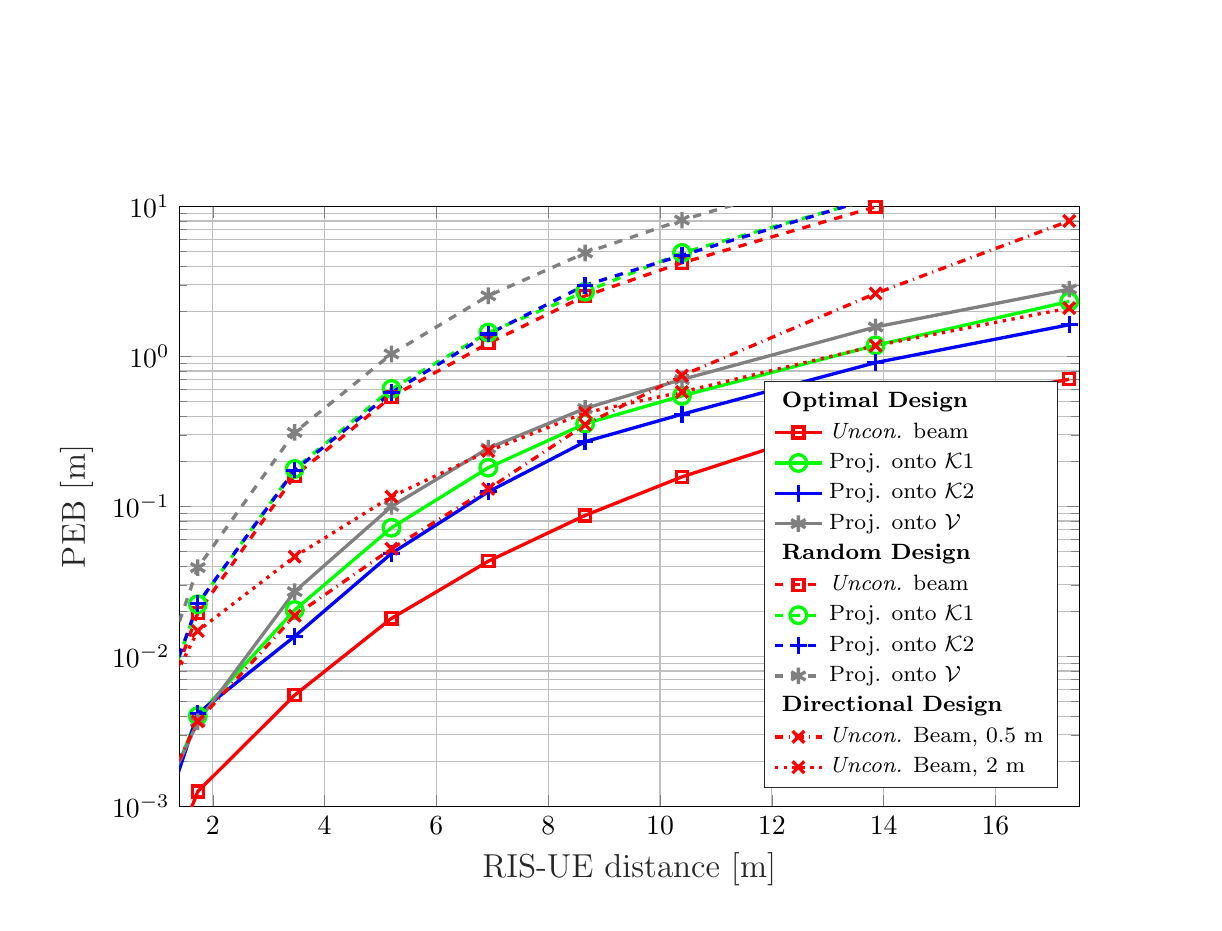
\begin{tikzpicture}

\begin{axis}[%
width=4.5in,
height=3in,
at={(0.758in,0.481in)},
scale only axis,
xmin=1.4,
xmax=17.5,
xlabel style={font=\large \color{white!15!black}},
xlabel={RIS-UE distance $[\mathrm{m}]$},
ymin=0.001,
ymax=10,
ylabel style={font=\large \color{white!15!black}},
ylabel={PEB $[\mathrm{m}]$},
yminorticks=true,
ymode = log,
axis background/.style={fill=white},
xmajorgrids,
yminorgrids,
legend style={font=\footnotesize, at={(0.65,0.03)}, anchor=south west, legend cell align=left, align=left, draw=white!15!black}
]
\addlegendimage{empty legend}
\addlegendentry{\hspace{-.6cm}\textbf{Optimal Design}}
\addplot [color=red, line width=1.2pt, mark=square]
  table[row sep=crcr]{%
0.3464	  0.0000127\\
0.8660	  0.00019\\
1.7320	  0.00126\\
3.4641	  0.00552\\
5.1961	  0.01796\\
6.9282	  0.04316\\
8.6602	  0.08721\\
10.392	  0.15751\\
13.856	  0.41196\\
17.320	  0.70435\\
};
\addlegendentry{\emph{Uncon.} beam}

\addplot [color=green, line width=1.2pt, mark=o, mark size = 3]
  table[row sep=crcr]{%
0.3464            0.00016\\
0.8660            0.00064\\
1.7320            0.00401\\
3.4641            0.02040\\
5.1961            0.07211\\
6.9282            0.18139\\
8.6602            0.35628\\
10.392            0.54593\\
13.856            1.18583\\
17.320            2.32581\\
};
\addlegendentry{Proj. onto $\mathcal{K}1$}
%
\addplot [color=blue, line width=1.2pt, mark=+, mark size = 3]
  table[row sep=crcr]{%
0.3464             0.00012\\
0.8660             0.00044\\
1.7320             0.00417\\
3.4641             0.01362\\
5.1961             0.04865\\
6.9282             0.12531\\
8.6602             0.27047\\
10.392             0.41203\\
13.856             0.90976\\
17.320             1.62787\\
};
\addlegendentry{Proj. onto $\mathcal{K}2$}
%
\addplot [color=gray, line width=1.2pt, mark=asterisk, mark size = 3]
  table[row sep=crcr]{%
0.3464          0.00016\\
0.8660      	0.00074\\
1.7320      	0.00367\\
3.4641      	0.02706\\
5.1961      	0.10009\\
6.9282      	0.24436\\
8.6602      	0.45048\\
10.392      	0.70239\\
13.856      	1.57218\\
17.320          2.81098\\
};
\addlegendentry{Proj. onto $\mathcal{V}$}
%
%
%
\addlegendimage{empty legend}
\addlegendentry{\hspace{-.6cm}\textbf{Random Design}}
\addplot [color=red, dashed, line width=1.2pt, mark=square, mark options = solid]
  table[row sep=crcr]{%
0.3464         0.00016\\
0.8660         0.00255\\
1.7320         0.01951\\
3.4641         0.15980\\
5.1961         0.53889\\
6.9282         1.22492\\
8.6602         2.53247\\
10.392         4.20990\\
13.856         9.92737\\
17.320         19.81937\\
};
\addlegendentry{ \emph{Uncon.} beam}
\addplot [color=green, dashed, line width=1.2pt, mark=o, mark options = solid, mark size = 3]
  table[row sep=crcr]{%
0.3464         0.00018\\
0.8660         0.00275\\
1.7320         0.02228\\
3.4641         0.17784\\
5.1961         0.60789\\
6.9282         1.44392\\
8.6602         2.70083\\
10.392         4.89874\\
13.856         11.44478\\
17.320         21.75501\\
};
\addlegendentry{Proj. onto $\mathcal{K}1$}
%
\addplot [color=blue, dashed, line width=1.2pt, mark=+, mark options = solid, mark size = 3]
  table[row sep=crcr]{%
0.3464         0.00019\\
0.8660      	0.00276\\
1.7320      	0.02251\\
3.4641      	0.17457\\
5.1961      	0.57451\\
6.9282      	1.40897\\
8.6602      	2.98439\\
10.392      	4.72464\\
13.856      	11.49018\\
17.320         22.39948\\
};
\addlegendentry{Proj. onto $\mathcal{K}2$}
%
\addplot [color=gray, dashed, line width=1.2pt, mark=asterisk, mark options = solid, mark size = 3]
  table[row sep=crcr]{%
0.3464          0.00025\\
0.8660      	0.00443\\
1.7320      	0.03914\\
3.4641      	0.31174\\
5.1961      	1.03910\\
6.9282      	2.53780\\
8.6602      	4.89841\\
10.392      	8.11626\\
13.856      	19.49614\\
17.320          37.75811\\
};
\addlegendentry{Proj. onto $\mathcal{V}$}
%
%
%
\addlegendimage{empty legend}
\addlegendentry{\hspace{-.6cm}\textbf{Directional Design}}
\addplot [color=red, dashdotted, line width=1.2pt, mark=x, mark size=3, mark options={solid}]
  table[row sep=crcr]{%
0.3464                0.0001\\%0.0005\\
0.8660      	      0.0008\\%0.0037\\
1.7320      	      0.0037\\%0.0054\\
3.4641      	      0.0187\\%0.0234\\
5.1961      	      0.0523\\%0.0627\\
6.9282      	      0.1309\\%0.1153\\
8.6602      	      0.3506\\%0.2915\\
10.392      	      0.7456\\%0.6138\\
13.856      	      2.6302\\%2.3083\\
17.320                8.0080\\%5.8782\\
};
\addlegendentry{\emph{Uncon.} Beam, $0.5~\mathrm{m}$}
%
\addplot [color=red, dotted, line width=1.2pt, mark=x, mark size=3, mark options={solid}]
  table[row sep=crcr]{%
0.3464                 0.0002\\
0.8660      	       0.0034\\
1.7320      	       0.0148\\
3.4641      	       0.0463\\
5.1961      	       0.1163\\
6.9282      	       0.2341\\
8.6602      	       0.4214\\
10.392      	       0.5796\\
13.856      	       1.1805\\
17.320                 2.1020\\
};
\addlegendentry{\emph{Uncon.} Beam, $2~\mathrm{m}$}
    
\end{axis}

\begin{axis}[%
width=5.833in,
height=4.375in,
at={(0in,0in)},
scale only axis,
xmin=0,
xmax=1,
ymin=0,
ymax=1,
axis line style={draw=none},
ticks=none,
axis x line*=bottom,
axis y line*=left
]
\end{axis}
\end{tikzpicture}%}
    \caption[]%
    {PEB as a function of \ac{RIS}-\ac{UE} distance for ideal and designed localization-optimal RIS beams, constrained by the real look-up tables/projection sets of the 4 characterized hardware prototypes.}
    \label{fig:PEBdist}
\end{figure}
%
Regarding the localization-optimal phase design, which requires a weighed combination of $4$ distinct beams, performance now seems much more sensitive to beam pattern approximation than that in the random design case, while experiencing much higher performance degradation in comparison with the \emph{unconstrained} case. This performance gap looks relatively constant as the \ac{RIS}-\ac{UE} distance increases though. Moreover, as expected, set $\mathcal{K}2$ seems relatively better than $\mathcal{K}1$ which is also better than $\mathcal{V}$. Finally, another set of two curves related to directional \ac{RIS} profile design are shown with different uncertainty sphere radii ($0.5~\mathrm{m}$ and $2~\mathrm{m}$). We Notice that in general, the \ac{PEB} of the directional design lies in between the localization-optimal and the random once. Furthermore, distributing the positions in a smaller uncertainty sphere yields a \ac{PEB} close to that projected onto sets $\mathcal{K}1$ and $\mathcal{K}1$ in the localization-optimal design only at short distances but then degrades quickly as the \ac{RIS}-\ac{UE} distance increases. On the other hand, using the bigger sphere gives the opposite behavior, this is inline with the results presented in~\cite{Rahal_Localization-Optimal_RIS}.

Fig.~\ref{fig:PEBaz} shows the PEB evolution as a function of the azimuth angle (i.e., the \ac{RIS}-\ac{UE} distance and elevation being fixed), where one can observe the same trends and ranking as before with the \ac{RIS}-\ac{UE} range. %However, the performance with set $\mathcal{V}$ looks strongly asymmetric, again likely due to the asymmetric/shifted distribution of the feasible reflection coefficients in the complex plane. \textcolor{magenta}{[If this is really the reason to invoke here, then why don't we see a similar PEB asymmetry as a function of the other elevation angle ?]}
Whatever the setting, the \ac{PEB} is also mainly better in the inner part of the spanned angular interval, illustrating typical geometric effects as we get away from the boresight, regardless of beam approximation. Since the \ac{RIS}-\ac{UE} distance is short, utilizing a directional phase design with a smaller sphere yields a better performance than a bigger one which in turn almost performs as the random design.
%
\begin{figure}[ht]
    \centering
    \resizebox{\columnwidth}{!}{% This file was created by matlab2tikz.
%
%The latest updates can be retrieved from
%  http://www.mathworks.com/matlabcentral/fileexchange/22022-matlab2tikz-matlab2tikz
%where you can also make suggestions and rate matlab2tikz.
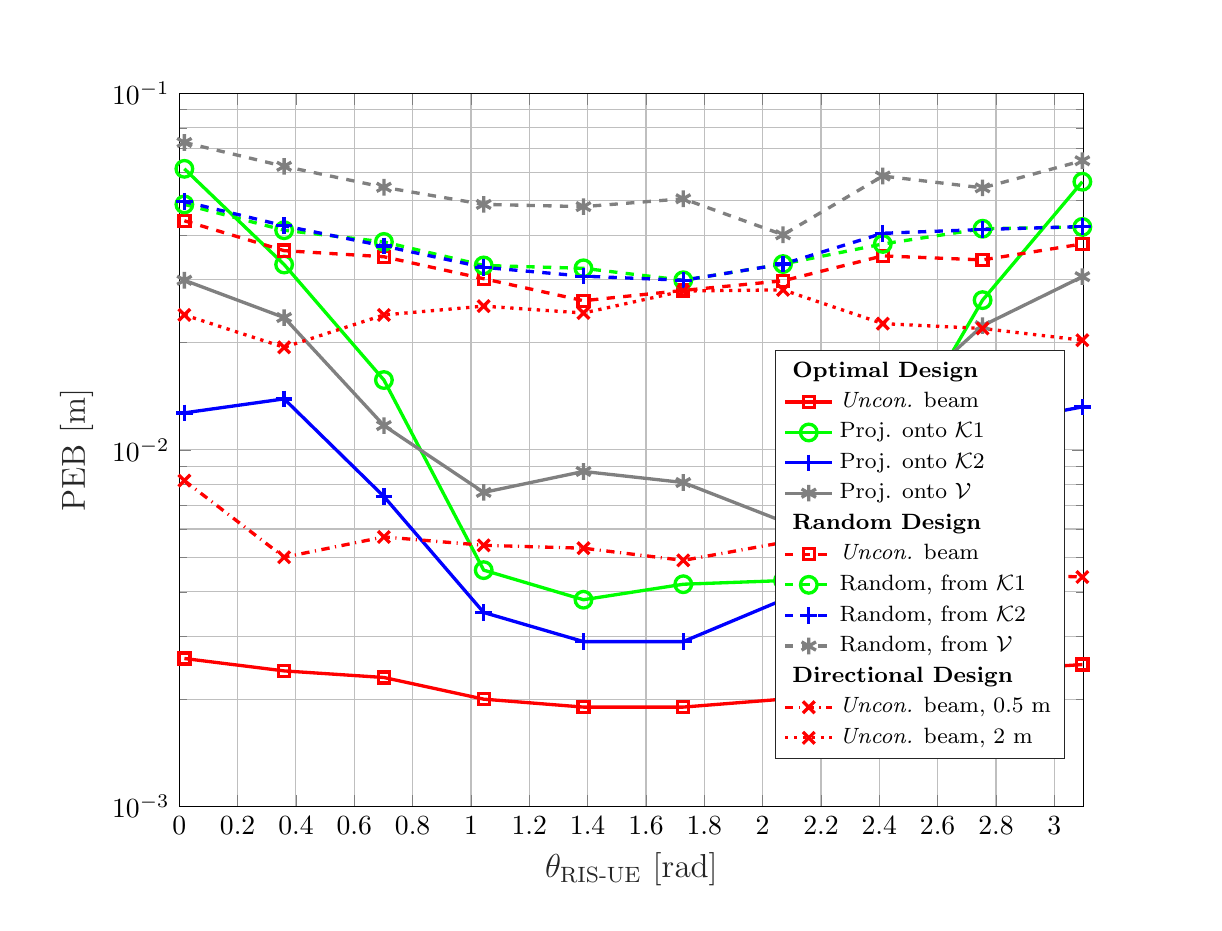
\begin{tikzpicture}

\begin{axis}[%
width=4.521in,
height=3.566in,
at={(0.758in,0.481in)},
scale only axis,
xmin=0,
xmax=3.1,
xlabel style={font=\large \color{white!15!black}},
xlabel={$\theta_{\text{RIS-UE}}~[\mathrm{rad}]$},
ymin=0.001,
ymax=0.1,
ymode = log,
ylabel style={font=\large \color{white!15!black}},
ylabel={PEB $[\mathrm{m}]$},
axis background/.style={fill=white},
xmajorgrids,
yminorgrids,
legend style={font = \footnotesize, at={(0.98,0.64)},legend cell align=left, align=left, draw=white!15!black}
]
%
\addlegendimage{empty legend}
\addlegendentry{\hspace{-.6cm}\textbf{Optimal Design}}
\addplot [color=red, line width=1.2pt, mark=square]
  table[row sep=crcr]{%
0.0175              0.0026\\% 0.00228\\
0.3595              0.0024\\% 0.00187\\
0.7016              0.0023\\% 0.00177\\
1.0437              0.0020\\% 0.00162\\
1.3858              0.0019\\% 0.00152\\
1.7279              0.0019\\% 0.00152\\
2.0700	            0.0020\\%  0.00161\\
2.4120	            0.0023\\%  0.00176\\
2.7541	            0.0024\\%  0.00186\\
3.0962	            0.0025\\%  0.00196\\
};
\addlegendentry{\emph{Uncon.} beam}

\addplot [color=green, line width=1.2pt, mark=o, mark size = 3]
  table[row sep=crcr]{%
0.0175           0.0614\\%  0.06553\\
0.3595           0.0331\\%    0.05311\\
0.7016           0.0157\\%    0.00928\\
1.0437           0.0046\\%    0.00616\\
1.3858           0.0038\\%    0.01306\\
1.7279           0.0042\\% 0.00416\\
2.0700	         0.0043\\%     0.00797\\
2.4120	         0.0087\\%     0.00959\\
2.7541	         0.0263\\%     0.03837\\
3.0962	         0.0565\\%     0.03728\\
};
\addlegendentry{Proj. onto $\mathcal{K}1$}

\addplot [color=blue, line width=1.2pt, mark=+, mark size = 3]
  table[row sep=crcr]{%
0.0175          0.0127\\%   0.01404\\
0.3595          0.0139\\%     0.02902\\
0.7016          0.0074\\%     0.00571\\
1.0437          0.0035\\%     0.00352\\
1.3858          0.0029\\%     0.00278\\
1.7279          0.0029\\%  0.00269\\
2.0700	        0.0038\\%      0.00391\\
2.4120	        0.0066\\%      0.00928\\
2.7541	        0.0117\\%      0.01747\\
3.0962	        0.0132\\%      0.01218\\
};
\addlegendentry{Proj. onto $\mathcal{K}2$}

\addplot [color=gray, line width=1.2pt, mark=asterisk, mark size = 3]
  table[row sep=crcr]{%
0.0175          0.0299\\% 0.15088\\
0.3595          0.0235\\% 0.04878\\
0.7016          0.0117\\% 0.01363\\
1.0437          0.0076\\% 0.00595\\
1.3858          0.0087\\% 0.02327\\
1.7279          0.0081\\% 0.00592\\
2.0700	        0.0063\\% 0.01357\\
2.4120	        0.0124\\% 0.01495\\
2.7541	        0.0223\\% 0.04852\\
3.0962	        0.0306\\% 0.08825\\
};
\addlegendentry{Proj. onto $\mathcal{V}$}
%
%
%
\addlegendimage{empty legend}
\addlegendentry{\hspace{-.6cm}\textbf{Random Design}}
\addplot [color=red, dashed, line width=1.2pt, mark=square, mark options={solid}]
  table[row sep=crcr]{%
0.0175               0.0439\\%0.04125\\
0.3595               0.0362\\%0.03537\\
0.7016               0.0348\\%0.03529\\
1.0437               0.0302\\%0.02962\\
1.3858               0.0262\\%0.02665\\
1.7279               0.0280\\%0.02542\\
2.0700	             0.0298\\%0.02897\\
2.4120	             0.0350\\%0.03151\\
2.7541	             0.0341\\%0.03779\\
3.0962	             0.0378\\%0.03877\\
};
\addlegendentry{\emph{Uncon.} beam}

\addplot [color=green, dashed, line width=1.2pt, mark=o, mark size=3, mark options={solid}]
  table[row sep=crcr]{%
0.0175               0.0488\\%0.04899\\
0.3595               0.0413\\%0.04064\\
0.7016               0.0383\\%0.03865\\
1.0437               0.0329\\%0.03296\\
1.3858               0.0323\\%0.02860\\
1.7279               0.0299\\%0.02870\\
2.0700	             0.0332\\%0.03166\\
2.4120	             0.0378\\%0.03774\\
2.7541	             0.0417\\%0.04108\\
3.0962	             0.0422\\%0.04340\\
};
\addlegendentry{Random, from $\mathcal{K}1$}

\addplot [color=blue, dashed, line width=1.2pt, mark=, mark=+, mark size=3, mark options={solid}]
  table[row sep=crcr]{%
0.0175                0.0497\\%0.04766\\
0.3595                0.0425\\%0.03959\\
0.7016                0.0373\\%0.03673\\
1.0437                0.0325\\%0.03323\\
1.3858                0.0307\\%0.02928\\
1.7279                0.0299\\%0.03013\\
2.0700	              0.0332\\%0.03044\\
2.4120	              0.0405\\%0.03886\\
2.7541	              0.0415\\%0.03925\\
3.0962	              0.0423\\%0.04221\\
};
\addlegendentry{Random, from $\mathcal{K}2$}

\addplot [color=gray, dashed, line width=1.2pt, mark=asterisk, mark size=3, mark options={solid}]
  table[row sep=crcr]{%
0.0175                0.0728\\% 0.07951\\
0.3595                0.0624\\% 0.07107\\
0.7016                0.0545\\% 0.05755\\
1.0437                0.0488\\% 0.04589\\
1.3858                0.0481\\% 0.04325\\
1.7279                0.0506\\% 0.04125\\
2.0700	              0.0401\\% 0.04431\\
2.4120	              0.0586\\% 0.06060\\
2.7541	              0.0543\\% 0.06803\\
3.0962	              0.0647\\% 0.07033\\
};
\addlegendentry{Random, from $\mathcal{V}$}
%
%
%
\addlegendimage{empty legend}
\addlegendentry{\hspace{-.6cm}\textbf{Directional Design}}
\addplot [color=red, dashdotted, line width=1.2pt, mark=x, mark size=3, mark options={solid}]
  table[row sep=crcr]{%
0.0175             0.0082\\% 0.0083\\
0.3595             0.0050\\% 0.0044\\
0.7016             0.0057\\% 0.0056\\
1.0437             0.0054\\% 0.0054\\
1.3858             0.0053\\% 0.0053\\
1.7279             0.0049\\% 0.0048\\
2.0700	           0.0055\\% 0.0058\\
2.4120	           0.0057\\% 0.0057\\
2.7541	           0.0045\\% 0.0055\\
3.0962	           0.0044\\% 0.0043\\
};
\addlegendentry{\emph{Uncon.} beam, $0.5~\mathrm{m}$}
%
\addplot [color=red, dotted, line width=1.2pt, mark=x, mark size=3, mark options={solid}]
  table[row sep=crcr]{%
0.0175              0.0239\\
0.3595              0.0194\\
0.7016              0.0239\\
1.0437              0.0253\\
1.3858              0.0242\\
1.7279              0.0279\\
2.0700	            0.0281\\
2.4120	            0.0226\\
2.7541	            0.0219\\
3.0962	            0.0203\\
};
\addlegendentry{\emph{Uncon.} beam, $2~\mathrm{m}$}

\end{axis}

\begin{axis}[%
width=5.833in,
height=4.375in,
at={(0in,0in)},
scale only axis,
xmin=0,
xmax=1,
ymin=0,
ymax=1,
axis line style={draw=none},
ticks=none,
axis x line*=bottom,
axis y line*=left
]
\end{axis}
\end{tikzpicture}%}
    \caption[]%
    {PEB as a function of \ac{RIS}-\ac{UE} azimuth angle for ideal and designed localization-optimal RIS beams, constrained by the real look-up tables/projection sets of the 4 characterized hardware prototypes.}
    \label{fig:PEBaz}
\end{figure}
%
Likewise, Fig.~\ref{fig:PEBel} shows similar \ac{PEB} curves as a function of the elevation angle (i.e., the \ac{RIS}-\ac{UE} distance and azimuth being fixed), where performance is still better in the inner part of the spanned angular intervals, illustrating typical effects as we get away from the boresight. The gap between the \ac{PEB} performance achieved with an \emph{unconstrained} beam pattern and its \emph{constrained} approximated variants seems all the more critical in those outer angular zones.
%
\begin{figure}[ht]
     \centering
     \resizebox{\columnwidth}{!}{% This file was created by matlab2tikz.
%
%The latest updates can be retrieved from
%  http://www.mathworks.com/matlabcentral/fileexchange/22022-matlab2tikz-matlab2tikz
%where you can also make suggestions and rate matlab2tikz.
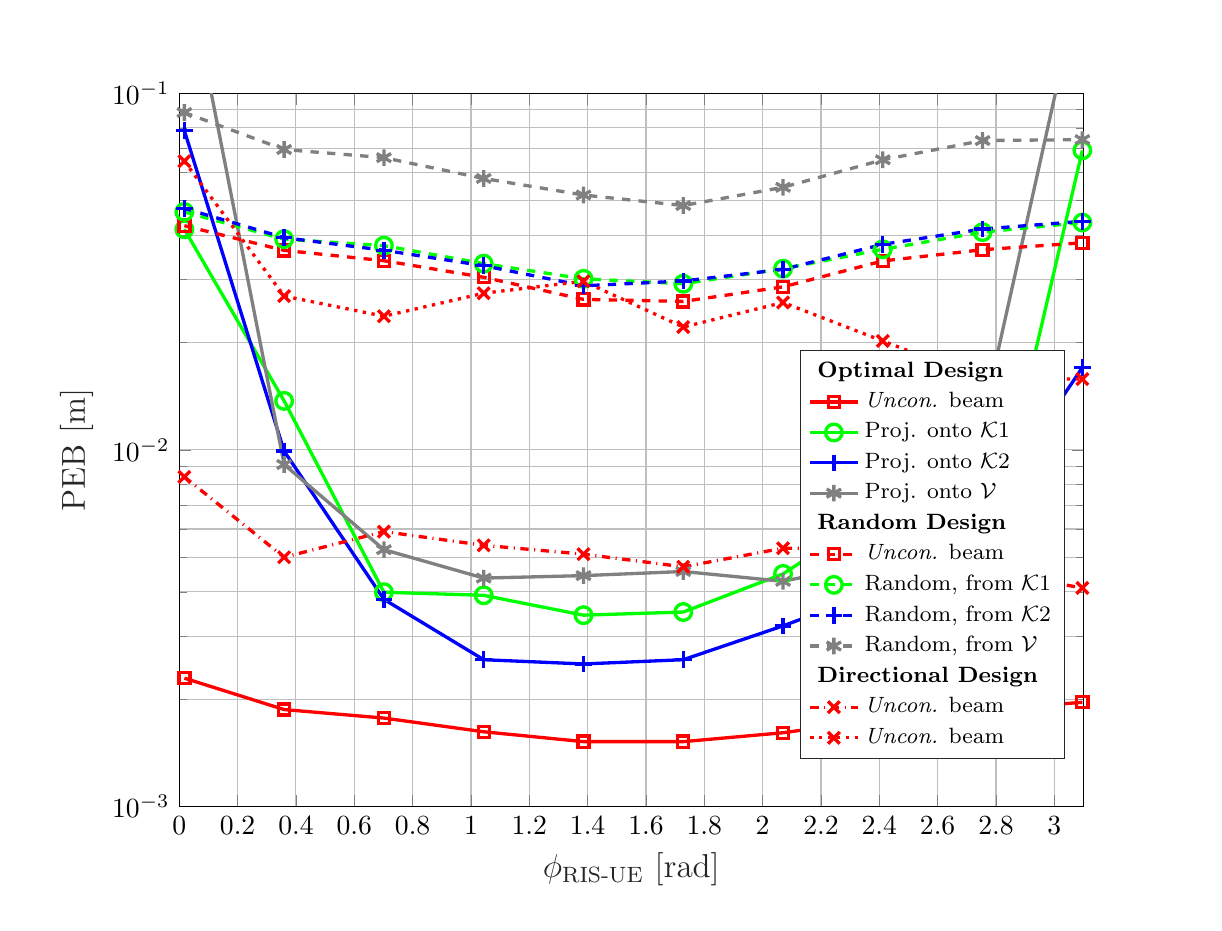
\begin{tikzpicture}

\begin{axis}[%
width=4.521in,
height=3.566in,
at={(0.758in,0.481in)},
scale only axis,
xmin=0,
xmax=3.1,
xlabel style={font=\large \color{white!15!black}},
xlabel={$\phi_{\text{RIS-UE}}~[\mathrm{rad}]$},
ymin=0.001,
ymax=0.1,
ymode = log,
ylabel style={font=\large \color{white!15!black}},
ylabel={PEB $[\mathrm{m}]$},
axis background/.style={fill=white},
xmajorgrids,
yminorgrids,
legend style={font=\footnotesize, at={(0.98,0.64)}, legend cell align=left, align=left, draw=white!15!black}
]
\addlegendimage{empty legend}
\addlegendentry{\hspace{-.6cm}\textbf{Optimal Design}}
\addplot [color=red, line width=1.2pt, mark=square]
  table[row sep=crcr]{%
0.0175      0.00229\\
0.3595      0.00187\\
0.7016      0.00177\\
1.0437      0.00162\\
1.3858      0.00152\\
1.7279      0.00152\\
2.0700      0.00161\\
2.4120      0.00176\\
2.7541      0.00186\\
3.0962      0.00196\\
};
\addlegendentry{\emph{Uncon.} beam}

\addplot [color=green, line width=1.2pt,, mark=o, mark size = 3]
  table[row sep=crcr]{%
0.0175      0.04155\\
0.3595      0.01372\\
0.7016      0.00399\\
1.0437      0.00391\\
1.3858      0.00344\\
1.7279      0.00351\\
2.0700      0.00449\\
2.4120      0.00684\\
2.7541      0.00436\\
3.0962      0.06917\\
};
\addlegendentry{Proj. onto $\mathcal{K}1$}

\addplot [color=blue, line width=1.2pt, mark=+, mark size = 3]
  table[row sep=crcr]{%
0.0175          0.07857\\
0.3595          0.00992\\
0.7016          0.00381\\
1.0437          0.00258\\
1.3858          0.00251\\
1.7279          0.00258\\
2.0700          0.00321\\
2.4120          0.00408\\
2.7541          0.00655\\
3.0962          0.01702\\
};
\addlegendentry{Proj. onto $\mathcal{K}2$}

\addplot [color=gray, line width=1.2pt, mark=asterisk, mark size = 3]
  table[row sep=crcr]{%
0.0175          0.24236\\
0.3595          0.00910\\
0.7016          0.00525\\
1.0437          0.00437\\
1.3858          0.00444\\
1.7279          0.00456\\
2.0700          0.00428\\
2.4120          0.00489\\
2.7541          0.01210\\
3.0962          0.21846\\
};
\addlegendentry{Proj. onto $\mathcal{V}$}
%
%
%
\addlegendimage{empty legend}
\addlegendentry{\hspace{-.6cm}\textbf{Random Design}}
\addplot [color=red, dashed, line width=1.2pt, mark=square, mark options = solid]
  table[row sep=crcr]{%
0.0175         0.04253\\
0.3595      0.03627\\
0.7016      0.03392\\
1.0437      0.03048\\
1.3858      0.02643\\
1.7279         0.02608\\
2.0700     	0.02865\\
2.4120     	0.03387\\
2.7541     	0.03642\\
3.0962     	0.03808\\
};
\addlegendentry{\emph{Uncon.} beam}

\addplot [color=green, dashed, line width=1.2pt, mark=o, mark options = solid, mark size = 3]
  table[row sep=crcr]{%
0.0175         0.04648\\
0.3595      0.03899\\
0.7016      0.03739\\
1.0437      0.03329\\
1.3858      0.03018\\
1.7279         0.02924\\
2.0700     	0.03222\\
2.4120     	0.03652\\
2.7541     	0.04079\\
3.0962     	0.04342\\
};
\addlegendentry{Random, from $\mathcal{K}1$}

\addplot [color=blue, dashed, line width=1.2pt, mark=+, mark options = solid, mark size = 3]
  table[row sep=crcr]{%
0.0175      0.04756\\
0.3595   0.03937\\
0.7016   0.03629\\
1.0437   0.03285\\
1.3858   0.02885\\
1.7279      0.02976\\
2.0700   0.03207\\
2.4120   0.03771\\
2.7541   0.04162\\
3.0962   0.04375\\
};
\addlegendentry{Random, from $\mathcal{K}2$}

\addplot [color=gray, dashed, line width=1.2pt, mark=asterisk, mark options = solid, mark size = 3]
  table[row sep=crcr]{%
0.0175         0.08832\\
0.3595      0.06956\\
0.7016      0.06599\\
1.0437      0.05770\\
1.3858      0.05184\\
1.7279         0.04844\\
2.0700      0.05449\\
2.4120      0.06509\\
2.7541      0.07371\\
3.0962      0.07413\\
};
\addlegendentry{Random, from $\mathcal{V}$}
%
%
%
\addlegendimage{empty legend}
\addlegendentry{\hspace{-.6cm}\textbf{Directional Design}}
\addplot [color=red, dashdotted, line width=1.2pt, mark=x, mark size=3, mark options={solid}]
  table[row sep=crcr]{%
0.0175            0.0084\\
0.3595            0.0050\\
0.7016            0.0059\\
1.0437            0.0054\\
1.3858            0.0051\\
1.7279            0.0047\\
2.0700   	      0.0053\\
2.4120   	      0.0053\\
2.7541   	      0.0046\\
3.0962   	      0.0041\\
};
\addlegendentry{\emph{Uncon.} beam}
%
\addplot [color=red, dotted, line width=1.2pt, mark=x, mark size=3, mark options={solid}]
  table[row sep=crcr]{%
0.0175                  0.0645\\%0.0292\\
0.3595                  0.0270\\%0.0180\\
0.7016                  0.0237\\%0.0270\\
1.0437                  0.0275\\%0.0243\\
1.3858                  0.0297\\%0.0234\\
1.7279                  0.0221\\%0.0327\\
2.0700   	            0.0259\\%0.0294\\
2.4120   	            0.0202\\%0.0298\\
2.7541   	            0.0158\\%0.0202\\
3.0962   	            0.0158\\%0.0223\\
};
\addlegendentry{\emph{Uncon.} beam}

\end{axis}
%%% angles in radians
%0.017
%0.357
%0.698
%1.038
%1.378
%1.719
%2.059
%2.399
%2.740
%3.080
\begin{axis}[%
width=5.833in,
height=4.375in,
at={(0in,0in)},
scale only axis,
xmin=0,
xmax=1,
ymin=0,
ymax=1,
axis line style={draw=none},
ticks=none,
axis x line*=bottom,
axis y line*=left
]
\end{axis}
\end{tikzpicture}%}
    \caption[]%
    {PEB as a function of \ac{RIS}-\ac{UE} elevation angle for ideal and designed localization-optimal RIS beams, constrained by the real look-up tables/projection sets of the 4 characterized hardware prototypes.}
    \label{fig:PEBel}
\end{figure}
%
% -------------------------------------------
% -------------------------------------------
\section*{Conclusion and Future Work}
%todo{Check and possibly make more precise.}
%
In this study, we presented a low-complexity technique for optimizing the complex configuration of \acp{RIS} so as to create various beam patterns, while considering real hardware limitations. The proposed method utilizes a pre-determined lookup table of possible \ac{RIS} element reflection coefficients, characterized out of real measurements. %Examples of directional and derivative beam patterns were also illustrated while taking into account gradual hardware constraints (including that of four real \ac{RIS} prototypes currently under development).
%
Applying the proposed beam generation strategy into the concrete context of \ac{NF} \ac{NLoS} localization, the performance degradation induced by beams approximation has then been evaluated in terms of both beam fidelity and \ac{PEB}, and further benchmarked for different a priori \ac{RIS} control strategies (incl. random, directional and localization-optimal designs). First numerical simulations regarding beam fidelity emphasize the dominating influence of both phase quantization levels (and the span of practically valid phases) and power losses regarding the element-wise complex reflection coefficients on the power gain of the \ac{RIS} beam peak in the desired \ac{UE} direction, as well as on the existence of unwanted secondary lobes. Other simulations performed in a canonical scenario also reveal the effects of beam synthesis and their relative power losses on the localization performance of different \ac{RIS} prototypes. The \ac{PEB} metric was utilized for that manner and the positioning was evaluated versus both \ac{RIS}-\ac{UE} distance and angles (i.e., both azimuth and elevation) to ensure that the study covers all the possible dimensions. As expected, constraining the beam synthesis to \ac{RIS} designs with certain limits degrade the positioning performance across all dimensions with various \ac{RIS} profile designs.
%\textcolor{magenta}{[To be completed once the latest PEB results are stabilized and analyzed.]}

Future works should investigate more \ac{RIS} prototypes by testing their different design characteristics based on localization performance. Extending the results to state-of-the-art as well as novel localization algorithms is also a possible path where the gaps in the performance of the \ac{RIS} devices can be analyzed and fixed.
%the practical performance of RIS-empowered multi-user communications, localization, and sensing at system level, while applying the proposed method under realistic hardware constraints (rather than restricting the study to beam patterns only), as well as the design of new \ac{RIS} hardware prototypes offering even more suitable feasible complex sets, whose distribution in the complex plane shall typically be centered and as close as possible to the unit circle. Moreover, a more in-depth quantitative analysis and comparison with the least-squares beamforming algorithm of \cite{tranter2017} needs to be performed.} 

\


%\subsection*{Sub-heading for section}
%Text for this sub-heading\ldots
%
%\subsubsection*{Sub-sub heading for section}
%Text for this sub-sub-heading\ldots
%
%\paragraph*{Sub-sub-sub heading for section}

%In this section\ldots
%
%\[
%E \bigl[Z_1(vT_x) \bigr]=
%\int_0^{v\wedge
%1}Z_0(uT_x)
%\exp (\lambda_1)\,du .
%\]
%
%\begin{equation}\label{eqexpmuts}
%\begin{aligned}[b]
%&      E\bigl[Z_1(vT_x)\bigr]\\
%&\quad      = \frac{\mu}{r}\log x
%\int_0^{v\wedge1}x^{1-u}x^{({\lambda_1}/{r})(v-u)}\,du .
%\end{aligned}
%\end{equation}
%

%\section*{Appendix}
%Blabla

%%%%%%%%%%%%%%%%%%%%%%%%%%%%%%%%%%%%%%%%%%%%%%
%%                                          %%
%% Backmatter begins here                   %%
%%                                          %%
%%%%%%%%%%%%%%%%%%%%%%%%%%%%%%%%%%%%%%%%%%%%%%

\section*{Acknowledgements}
The authors would like to warmly thank Dr. Antonio Clemente, from CEA-Leti, France, Dr. Philippe Ratajczak, from Orange Innovation Networks, France, for sharing the look-up tables associated to their R-RIS hardware prototypes in the context of RISE-6G project, as well as for the fruitful technical discussions and the relevant advice regarding this paper.

\section*{Funding}%% if any
This work has been supported, in part, by the EU H2020
RISE-6G project under grant 101017011 and by the MSCA-IF
grant 888913 (OTFS-RADCOM).

\section*{Abbreviations}%% if any
\begin{itemize}
\item BS: Base Station
\item DoD: Direction of Departure
\item FIM: Fisher Information Matrix
\item LoS: Line-of-Sight
\item LMI: Linear Matrix Inequalities
\item MC: Multi-Carrier
\item MIMO: Multiple Inputs Multiple Outputs
\item NF: Nearfield
\item NLoS: Non-Line-of-Sight
\item OEB: Orientation Error Bound
\item PEB: Position Error Bound
\item PSD: Positive Semi Definite
\item RIS: Reconfigurable Intelligent Surface
\item QoS: Quality of Service
\item RX: Receiver
\item SDP: Semi Definite Program
\item S(I)NR: Signal-to-(Interference-and-)Noise-Ratio
\item SISO: Single-Input-Single-Output
\item SRE: Smart Radio Environment
\item UE: User Equipment
\item TDoA: Time Difference of Arrival
\item TX: Transmitter
\end{itemize}

%%%%%%%%%%%%%%%%%%%%%%%%%%%%%%%%%%%%%%%%%%%%%%%%%%%%%%%%%%%%%
%%                  The Bibliography                       %%
%%                                                         %%
%%  Bmc_mathpys.bst  will be used to                       %%
%%  create a .BBL file for submission.                     %%
%%  After submission of the .TEX file,                     %%
%%  you will be prompted to submit your .BBL file.         %%
%%                                                         %%
%%                                                         %%
%%  Note that the displayed Bibliography will not          %%
%%  necessarily be rendered by Latex exactly as specified  %%
%%  in the online Instructions for Authors.                %%
%%                                                         %%
%%%%%%%%%%%%%%%%%%%%%%%%%%%%%%%%%%%%%%%%%%%%%%%%%%%%%%%%%%%%%

% if your bibliography is in bibtex format, use those commands:
\bibliographystyle{bmc-mathphys} % Style BST file (bmc-mathphys, vancouver, spbasic).
\bibliography{bmc_article}      % Bibliography file (usually '*.bib' )
\end{document}
